\documentclass[conference]{IEEEtran}
%\IEEEoverridecommandlockouts
% The preceding line is only needed to identify funding in the first footnote. If that is unneeded, please comment it out.
\usepackage{cite}
\usepackage{amsmath,amssymb,amsfonts}
\usepackage{algorithmic}
\usepackage{graphicx}
\usepackage{textcomp}
\usepackage{xcolor}
\usepackage{mathtools}
\usepackage{pgfplots}
\pgfplotsset{compat=1.18}
\usepackage{pgfplotstable}
\usetikzlibrary{patterns}

\usepackage{cleveref}
\usepackage{url}
\usepackage{tikz}
\usetikzlibrary{shapes,arrows,positioning,fit}

\def\BibTeX{{\rm B\kern-.05em{\sc i\kern-.025em b}\kern-.08em
    T\kern-.1667em\lower.7ex\hbox{E}\kern-.125emX}}
\begin{document}
\urlstyle{tt}
\title{Improving Domestic Abuse Support in the UK: Automating Discovery of Aid Services through Web Crawling

%\thanks{Identify applicable funding agency here. If none, delete this.}
}

\author{\IEEEauthorblockN{1\textsuperscript{st} Stavros Michalovits}
\IEEEauthorblockA{\scalebox{.9}[1.0]{\textit{School of Computer Science}} \\
\scalebox{.9}[1.0]{\textit{University of St Andrews}}\\
St Andrews, Scotland \\
sm519@st-andrews.ac.uk}
\and
\IEEEauthorblockN{2\textsuperscript{nd} Annah McCurry}
\IEEEauthorblockA{\scalebox{.9}[1.0]{\textit{School of Psychology \& Neuroscience}} \\
\scalebox{.9}[1.0]{\textit{University of St Andrews}}\\
St Andrews, Scotland \\
0000-0003-3403-7680}
\and
\IEEEauthorblockN{3\textsuperscript{rd} Ruth Hoffmann}
\IEEEauthorblockA{\scalebox{.9}[1.0]{\textit{School of Computer Science}} \\
\scalebox{.9}[1.0]{\textit{University of St Andrews}}\\
St Andrews, Scotland \\
0000-0002-1011-5894}
\and
\IEEEauthorblockN{4\textsuperscript{th} Swithun Crowe}
\IEEEauthorblockA{\scalebox{.9}[1.0]{\textit{Research Computing}} \\
\scalebox{.9}[1.0]{\textit{University of St Andrews}}\\
St Andrews, Scotland \\
0000-0001-8485-8597}
\and
\IEEEauthorblockN{5\textsuperscript{th} Patrick McCann}
\IEEEauthorblockA{\scalebox{.9}[1.0]{\textit{Research Computing}} \\
\scalebox{.9}[1.0]{\textit{University of St Andrews}}\\
St Andrews, Scotland \\
0000-0002-9324-2775}
\and
\IEEEauthorblockN{6\textsuperscript{th} David I Donaldson}
\IEEEauthorblockA{\scalebox{.9}[1.0]{\textit{School of Psychology \& Neuroscience}} \\
\scalebox{.9}[1.0]{\textit{University of St Andrews}}\\
St Andrews, Scotland \\
0000-0002-8036-3455}
\and
\IEEEauthorblockN{7\textsuperscript{th} Bobby May}
\IEEEauthorblockA{\scalebox{.9}[1.0]{\textit{School of Psychology \& Neuroscience}} \\
\scalebox{.9}[1.0]{\textit{University of St Andrews}}\\
St Andrews, Scotland \\
0000-0001-8110-8408}
}

\maketitle

\begin{abstract}
We present the development of an automatically updating catalogue of services supporting Domestic Abuse survivors in Scotland and the United Kingdom. 
In particular, we employ a web crawler with a rules-based relevance model to discover services, flagging new services to human experts for review and allowing for a lighter workload for curating.
The system is designed for adaptability with regard to changes in terminology related to Domestic Abuse, both to aid maintenance and allow expansion to other regions.
\end{abstract}

\begin{IEEEkeywords}
web crawling, scraping, database, automatic, Domestic Abuse services
\end{IEEEkeywords}

\section{Introduction}

Since 2019, the Women's Aid Federation of England has received roughly \textsterling 1.2 million in funding from the UK government for their "Routes to Support" project\cite{wafin20, wafin21, wafin22}.
Central to the project is a database of Domestic Abuse services in the UK that is manually updated, multiple times a year. 
This database is a critical resource built for end users (people suffering Domestic Abuse), enabling them to identify services that can help them flee abuse and find safety. 
However, funding for Domestic Abuse services in the UK is volatile, and services appear and disappear every year due to funding availability. 
This makes the task of keeping a manual directory of services up-to-date onerous, time-consuming, and expensive. 
Most critically, outdated items in the directory threaten its usability for survivors who need to identify urgent assistance.

From the service provider's perspective (UK-based Domestic Abuse services, in this case), maintaining the database is not only time-consuming and expensive, but it is also difficult to judge the comprehensiveness and accuracy of the database. 
Specifically, there are so many different \textit{organisations} offering Domestic Abuse services (over 170 separate organisations in the UK alone, e.g., Women's Aid, Galop, Anah Project, etc.) and such volatile funding for both organisations and specific programmes that it is impossible to keep track of changes in programming over time. 
As of May, 2024, Women's Aid's directory attempts to keep information on 510 programmes up to date (where multiple locations for the same organisation are counted separately) \cite{wadir}.

The availability and correctness of such a service is crucial. 
Ideally, finding and curating new services (as well as removing ceased programmes) should be fully automated, to  lighten the manual burden of the day-to-day running of the database and service.

We have built a self-updating catalogue using web crawling and rules-based relevance models.
This is the first step which will enable the creation of a central resource and a Graphical User Interface that can be embedded into websites belonging to Domestic Abuse services, allowing survivors to find resources in their area that meet their needs and remove the database burden from service providers. 

Our resource creates a comprehensive list of Domestic Abuse concepts and vocabulary in consultation with Domestic Abuse Research and Impact Scotland (DARIS: \url{https://daris.wp.st-andrews.ac.uk/}) researchers and their contacts within Domestic Abuse services. 
This is being carefully designed into a database, which depends on a flexible design to integrate possible changes in vocabulary while remaining scalable to eventually cover services across the whole UK. 
Critically, our flexible framework will allow other public service sectors (both nationally and internationally; such as refugee services, etc.) to modify our approach and reproduce a database that serves their services and programmes.

We are presenting the first steps involved in the creation of this semi-automated web crawler and database resource (code and data: \url{https://github.com/smich42/st-andrews-dvsvc}).
This paper presents the workflow of how appropriate data is being found, curated and tagged ( \cref{sec:flow}). 
It then looks at the results for the web crawler and assesses the quality of the web pages found (\cref{sec:res}).
Finally, we will discuss the next steps of how the database of services will be presented and made accessible to end-users  (\cref{sec:future}).





\section{Workflow}
\label{sec:flow}
The creation of the services resource consists of multiple stages (\cref{fig:stages} shows their interplay), most of which run automatically. However, given the complex nature of determining relevance, some minor manual intervention (through Human Verifiers) in the creation of the Expert Lists and sanitisation of the data is needed before the data is made available to the public through a website.

Our goal is to make the resource flexible in terms of:
\begin{itemize}
    \item services; while we focus on Domestic Abuse services, the framework introduced can be easily repurposed for other critical services with a fast turn-around in programmes (such as homelessness services).
    \item languages/regions; the resource created focuses on English-language UK services, but this can be flexibly changed to any language or region (such as adding Welsh/Gaelic services to the UK list).
\end{itemize}
In the following sections we detail each of the stages of the framework (as presented in \cref{fig:stages}).

This paper focuses on the stages which curate the list of Domestic Abuse service webpages.
Future work (the grey stages in \cref{fig:stages}), which will be briefly discussed include turning the list of services webpages into a well-structured database, with effective queries aimed at the end user (Domestic Abuse survivors), a central graphical user interface, and an embeddable frontend which can be used by Domestic Abuse services on their webpages as well.

\begin{figure}
\begin{center}
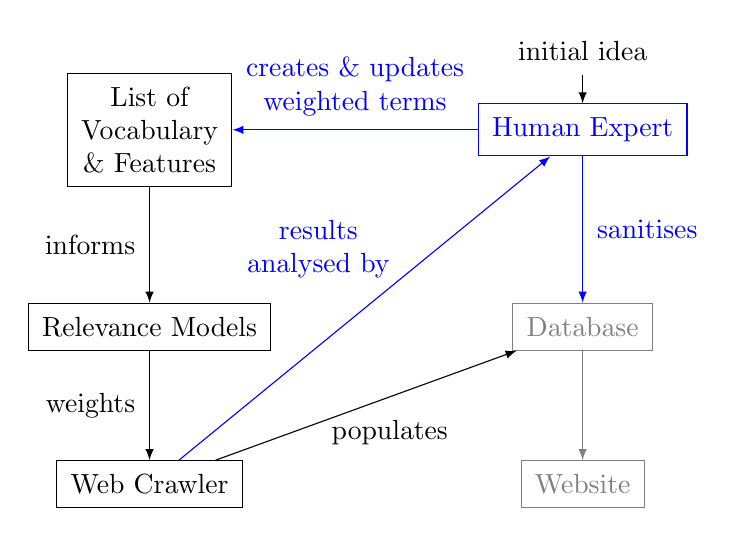
\begin{tikzpicture}[auto,on grid,>=latex,every node/.style={align=center,draw,rectangle,inner sep =5pt}]
\node[draw=none] (a) at (5.5,1) {initial idea};
\node (vocab) at (0,0) {List of \\Vocabulary \\ \& Features};
\node (model) at (0,-2.5) {Relevance Models};
\node (crawl) at (0,-4.5) {Web Crawler};
\node[color=blue] (verify) at (5.5,0) {Human Expert};
\node[color=gray] (db) at (5.5,-2.5) {\color{gray}{Database}};
\node[color=gray] (web) at (5.5,-4.5) {\color{gray}{Website}};

\draw[->] (vocab) edge node [draw = none,left] {informs} (model)
            (model) edge node [draw = none,left] {weights} (crawl)
            (crawl) edge node [draw = none,below,xshift=3mm] {populates} (db)
                edge [color = blue] node [draw=none,yshift=2mm,xshift=5mm] {results \\ analysed by} (verify)
            (verify) edge [color=blue] node [draw = none] {sanitises} (db)
                edge [color=blue] node [above,draw=none] {creates \& updates \\ weighted terms} (vocab)
            (db) edge [color=gray] (web)
            (a) edge (verify);

\end{tikzpicture}
\caption{All stages creating the resource. Blue shaded stages indicate manual interference. Grey shaded concepts are work-in-progress/future work.}
\label{fig:stages}
\end{center}
\end{figure}

\subsection{The Role of Human Experts}
\label{sec:verif}
Experts in Domestic Abuse are involved in the resource creation workflow in two crucial steps.
Firstly, they are involved in creating the service vocabulary/list which is used to inform the web crawler, and part of the initial sanitisation of items in the database.
Secondly, experts routinely need to check any changes in the data from the web crawler to identify if the data is compromised.

Identifying potential Domestic Abuse services and determining what should be included in a comprehensive directory is difficult for non-expert humans. 
For example, some organisations offer support that may cater to people with historical abuse (i.e., those who have suffered abuse but are not currently fleeing from it; e.g., The Haven Project\cite{haven}), but they are not themselves Domestic Abuse services.
Further, some commercial entities may have special offers for Domestic Abuse survivors (e.g., financial abuse support through banks, pro Bono legal work through private law firms, etc.), but these usually require referral through recognised or affiliated Domestic Abuse services, and thus are not the priority for a survivor-facing database \cite{enduser}.  
Moreover, many local council websites provide information on Domestic Abuse alongside a phone number, but it can be extremely difficult to determine if the phone number is associated with a one-off Domestic Abuse service or just a general inquiry line that will signpost to specific Domestic Abuse services. 
To illustrate this point, see the Thanet Council webpage on Domestic Abuse (\url{https://www.thanet.gov.uk/info-pages/domestic-abuse/}). 
At the time of writing, they provide a phone number to call in case of Domestic Abuse, heavily implying that they offer a one-off service. 
However, careful vetting of the phone number and associated project reveals that survivors are being referred to a homelessness service, not a Domestic Abuse service. 
This example shows precisely how important it is to develop a clear and simple database of relevant services for end users. 
It also demonstrates the necessity of (expert) human verification within the framework.
These and other practical decisions based on the needs of the end user make it essential to include experts in the design and verification process. Without them, the database may include so many false positives that it becomes functionally useless to end users.

The list of terminology and vocabulary, as well as their importance for a sensitive topic like ``UK Domestic Abuse services" must be created and configured by an expert. One possible solution could be the use of machine learning, but 
there are too few UK services for a machine learning binary-classifier model to train on.
The Women's Aid Directory numbers just 510 services.
There have been some attempts at using models to classify generic registered charities.
Damm \& Kane \cite{dammkane2021} achieved a maximum of 57\% accuracy in labelling registered UK charities across various machine learning models, with a substantially larger dataset (6,203 labelled charities) than is achievable in our domain---though this was a multi-label classifier. 
While Ma \cite{ma2020} achieved 90\% accuracy in multi-class classification, that is also with a large dataset of US nonprofit organisations and significantly more complex model. 
Crucially, our use case requires a degree of human judgement that, as discussed, is challenging for non-experts.

A manually informed approach is thus more appropriate, and still allows for the flexibility in the framework that we are aiming to achieve.
That means that we use the list of vocabulary and the knowledge of DARIS experts to infer weighted \textit{predicates} for each entry that can collectively identify Domestic Abuse services. 
We iteratively modified the predicates until the resulting provisional catalogue of webpages (often ambiguous as to whether they are relevant) contains an amount of websites which is reasonable to ask an expert to review.

Once the initial catalogue is labelled, continuing to run the crawler should only generate trivially small increments to the dataset as services appear or disappear (or, as will be discussed under \cref{sec:res}, iterative improvement of the system makes it more effective at finding services).
There is only a one-off large manual cost, that is reviewing the initial catalogue. 
Results must nonetheless be manually reviewed before they are published to end users---importantly, our system facilitates both reviewing and updating the catalogue with a trivial manual burden in comparison with current, fully manual, efforts.



\subsection{List of Vocabulary and Features}
\label{sec:vocab}
Our approach requires a list of terms and expressions curated by experts in the field who have researched the topic and service providers with practical knowledge. 
As mentioned, we specifically used DARIS and their community contacts in the present project\cite{theme}. 
This list needs to be constantly updated by the experts as the language around Domestic Abuse is fast evolving, which includes not only the addition of new terms but also the change in the meaning of older ones, with some long-standing terminology becoming obsolete or even inappropriate (e.g., ``Domestic Abuse" vs. ``Domestic Violence", where the latter is considered appropriate in England but not Scotland).

Each of the phrases generated by our experts is assigned a relative weight, which we formalise in \cref{relmod}.
For now, note that the weighting is initially determined by DARIS experts based on knowledge of what words or phrases strongly indicate that a given page represents a Domestic Abuse service in the region we are tackling.

In addition to vocabulary keywords, we look for particular features associated with Domestic Abuse services. 
The most notable are ``Quick Exit'' buttons: interactive elements that commonly appear on webpages servicing survivors of Domestic Abuse, particularly those needing to hide their browsing activity from their abuser. 
As \cref{fig:exit} shows, they are not standardised with respect to design and wording.
We look for clickable HTML elements labelled by a word such as ``leave", ``exit", along with either a mention of ``page", ``website", \textit{or} ``quick", ``now", and so on. 
In rare cases, the quick exit button will not explicitly contain text but rather an image or symbol, making it undetectable. Similarly, there are some one-off particular phrases used that are undetectable, but they are too infrequent to warrant the creation of a more complex model (for one, see Cornwall Refuge Trust in the middle of \cref{fig:exit}).

Another feature is charity codes.
Registers of Scottish and rest-of-the-UK (rUK) charity codes are published by the Scottish Charity Regulator (OSCR), Charity Commission for England and Wales, and Charity Commission for Northern Ireland \cite{scotchar, rukchar, nichar}.
Scottish charity codes are particularly useful because they are prefixed with ``SC" and thus easy to identify with very few spurious matches. 
Conversely, rUK charity codes are 6 or 7 digit integers and---critically---sequential. 
A page that contains a 6 or 7 digit number will therefore be found to correspond to some rUK charity (as long as the number is in the current range of charity numbers).
Distinguishing whether such a number that appears on a page indeed refers to an rUK charity is therefore unreliable.
Only Scottish charity codes are thus included in the list of vocabulary and features.

\begin{figure}
    \centering
    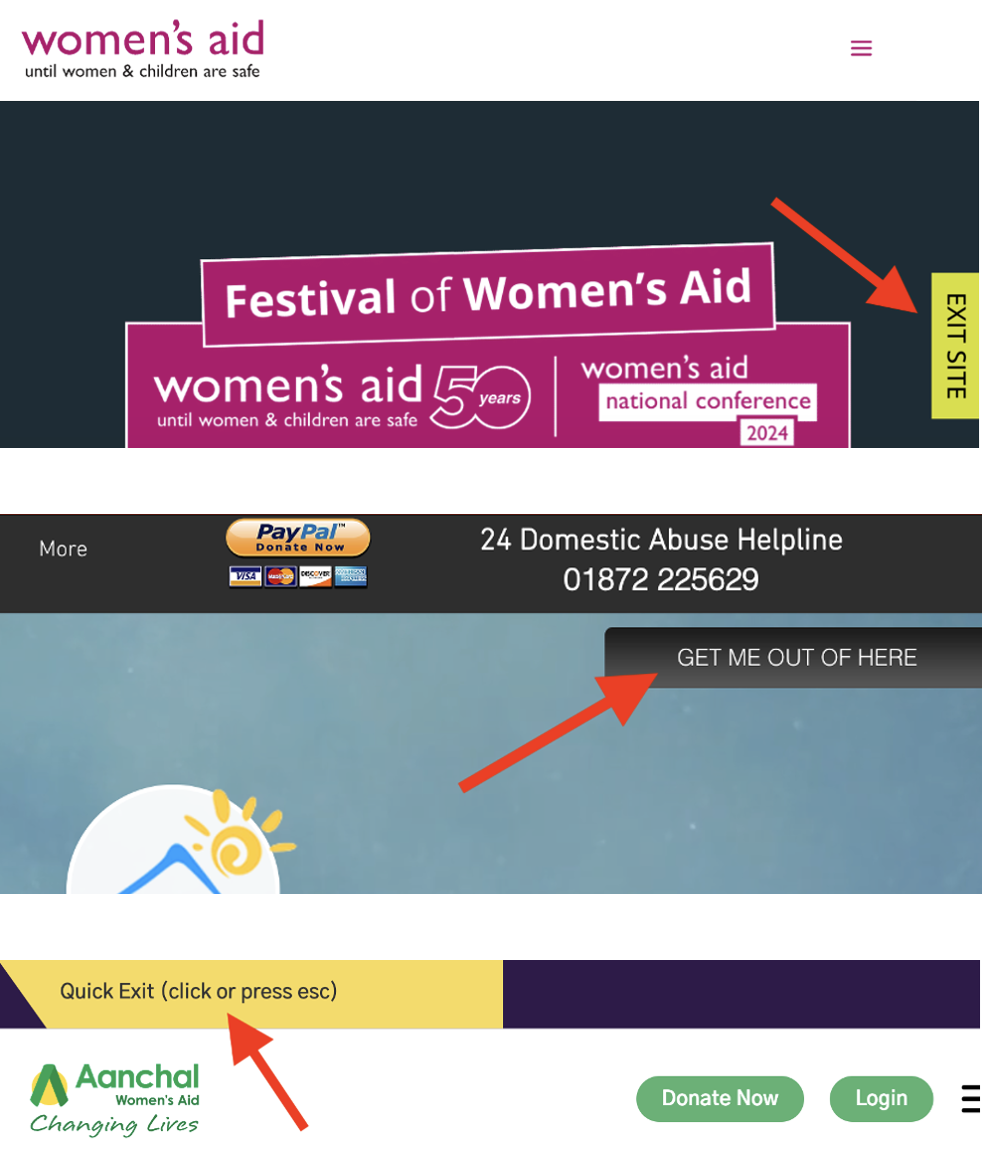
\includegraphics[width=1\linewidth]{quick-exit.png}
    \caption{Different Quick Exit buttons for Women's Aid UK \cite{wauk}, Cornwall Refuge Trust\cite{cornrt} and  Aanchal \cite{aanchalwa}, respectively.}
    \label{fig:exit}
\end{figure}

The list of vocabulary/terminology can be replaced with another to create a resource for other sectors (e.g., services for people experiencing homelessness, services for recent immigrants/refugees, etc.). 
But as discussed above, should the list be adapted, experts need to be consulted about the importance of terms and checks of the web crawler's initial results must be performed to ascertain performance and make modifications as need be. 

\subsection{Relevance Modelling}
\label{relmod}

Relevance modelling incorporates the list of vocabulary and features and serves two purposes to our workflow. First, it allows us to decide whether to \textit{itemise} a page, i.e., add it to the database. Second, it allows us to prioritise URLs that are more likely to link to relevant pages.

As such, there are two models involved in ranking webpages for their relevance. 
Both share the same underlying mathematical functions, but the \textit{link model} investigates URLs, while the \textit{page model} evaluated the HTML content of the pages. We will first discuss the mathematical foundations (which both models share), before delving into its impact on the two models.

A set of predicates is initially derived from the list of vocabulary and features. 
Each item in the list is translated into a regular expression predicate (e.g., matching the \url{.org.uk} top-level domain), an HTML lookup predicate (e.g., ``Quick Exit" buttons), or a keyword lookup predicate (e.g., the phrase ``intimate partner violence"). 

A keyword lookup predicate is a set of keyword sets along with an integer $n$, requiring $n$ terms of each keyword set to decide that the predicate is a match. 
For instance, to decide that a page is a news site we need both news-related terminology (e.g., ``news", ``headline") and enough general news topics to appear (e.g., ``politics", ``weather") --- which enables us to distinguish between news sites with pages about Domestic Abuse and Domestic Abuse sites with a ``news and announcements" (or similar) page.

For each predicate $p$ from our list of vocabulary we manually assigned two weights $c_p$ and $s_p$, a \textit{constant} and a \textit{scaling} weight respectively. 
As described in \cref{sec:vocab}, these values are based on expert judgement. 
We also use successive crawls to search for their optimal values. 
For example, the scaling effect of a Scottish charity code was initially set to relatively high value. 
Manually inspecting the predicates matched by false-positive pages revealed that this amplified charities that \textit{funded} Domestic Abuse services rather than \textit{ran} them. A reduced value thus reflected that Scottish charity status is a less reliable predictor of relevance than originally thought.

For an input $I$ (either an URL or the HTML content), and a set of predicates $P$ (the list of vocabulary and features), we calculate a score (which will lay in the interval $(-1,1)$) of the input as a logistic scale of the effects of the predicates' weights. Scores near -1 will indicate the overwhelming presence of predicates with negative effect, indicating irrelevance, while scores near 1 will indicate the overwhelming presence of positively weighted predicates, indicating relevance.

\begin{equation}
\begin{aligned}
\text{Score}(I, P) = & \sigma_{x_{90}}(\text{Compound}(I, P) \\ 
& +\gamma\text{WordCount}(I))
\end{aligned}
\label{eq:score}
\end{equation}

where $x_{90}$ is the $x$-value needed for the 90th percentile of positive confidence and $\gamma$ is a non-positive word count factor, both derived through an initial judgement and iteration.
We define  $\sigma_{x_{90}}: \mathbb{R}\rightarrow (-1,1)$ to be the transformation of the standard logistic function that passes through $(0, 0)$ and the point $(x_{90}, 0.90)$ with a supremum of 1.

The WordCount function counts how many words the input consists of. For a URL this will be 0, and for a page we remove markup elements such as HTML before counting.

The Compound function computes the cumulative effect of the constant and scaling factors of the matched predicates. So, for an input $I$ and a set of predicates $P$ it is 
\begin{equation}
\begin{aligned}
\text{Compound}(I, P) = & \left(\prod_{p\in P} s_p \text{ IsMatch}(I, p)\right) \\
& \times \left( \sum_{p\in P}c_p\text{ IsMatch}(I, p)\right)
\end{aligned}
\label{eq:comp}
\end{equation}

where IsMatch is a boolean function; if part of the input $I$ matches the predicate $p$ then we assign it the value $1$.

The word-count factor $\gamma$ is needed because wordy pages (e.g., ``Terms and Conditions" documents) tend to match more predicates irrespective of whether they are relevant overall. 
One approach is to divide the compounded weights by the word count and consider the predicate \textit{density} of a page. 
However, we found this approach to penalise some relevant websites; for instance, larger services may focus on more topics than Domestic Abuse, making their pages sparser in relevant keywords. 
A constant word-count factor avoids over-penalising relevant pages, while filtering out those who are so unusually wordy that they may match keyword predicates solely by chance.

Because Score is continuous (rather than, e.g., classifying 0/1 for relevant/irrelevant), it can be used in combination with \textit{meta-heuristics} to make a final decision on relevance. 
As will be discussed further, we may be confident that a particular website is relevant if it is dense in reasonably high-scoring pages even if no individual page has an exceptional score. 
A binary judgement of 0/1 by the scorer would not allow this flexibility on the part of the crawler.

The link model generates an \textit{lscore} (based on \cref{eq:score}) between -1 and 1 that indicates relevance to the ``broad topic" of our search: UK-based services, charities and organisations. 
The reason for the link model being ``broad" is that URL text is not enough information to classify the page it links to. 
We may be able to infer, for instance, that a given link refers to a British charity if it ends in \texttt{.org.uk} and matches the vocabulary words ``charity" and ``foundation"---but it is impossible to infer \textit{what} the charity is about, and our manual inspection of known Domestic Abuse services indicated that URLs do not consistently offer such granular insight.

This also means links are rarely penalised: URLs simply do not provide enough hints to confidently do so. 
Therefore, the lscore does not implement negative predicates, with the exception of regional Top-Level Domains of non-UK English-speaking nations, which are weighted as $-\infty$ to avoid visiting altogether. 
Negative lscores are thus rare.

The page model predicts whether a given page is a Domestic Abuse service; that is the \textit{pscore} of the page (again based on \cref{eq:score}). 
A pscore ranges between -1 and 1, where 1 indicates absolute certainty that the page is relevant and -1 that it is irrelevant.

Scaling and constant terms accumulate separately such that their effect is independent of the order in which they are matched. Crucially, scaling terms enable us to approximate a contextual understanding of different terms in the text---essentially, depending on its $s$-weight, a predicate can have a dampening or a amplifying effect on other predicates. For example, the predicate matching universities and academic journals was ultimately set a 0.7 scaling weight, dampening the effect of the keyphrase ``coercive control" by 30\% as informed by the fact that the mention is likely in an academic context. Conversely, matching a Scottish charity code has a 1.2 scaling weight, as it reveals that the page is contextually relevant.

In summary, \textit{pscore} is composed of predicates for the following:
\begin{itemize}
    \item Keyword and keyphrase matches.
    \item Presence of a ``Quick Exit" element.
    \item Charity codes.
\end{itemize}

\textit{lscore} similarly considers:
\begin{itemize}
    \item Keyword matches.
    \item Top-Level Domains (TLDs), e.g., \texttt{org.uk}.
    \item pscore of the \textit{parent page}, that is the page from which the link was obtained.
\end{itemize}

So far, we have discussed how we score pages on the likelihood that they offer services for Domestic Abuse survivors. 
However, we must also ensure that the Domestic Abuse services we identify are UK-based. 
A way of doing this would be to develop a set of localisation predicates for pscore. 
For instance, we could match regional linguistic hints such as spellings or idioms, place names and phone numbers in conjunction with \textit{whois} lookups. 
But a naive implementation of such a mechanism is bound to be inaccurate: spelling variants and place names are often duplicated across English-speaking nations (especially in the Commonwealth) and \textit{whois} can be anonymised (as it often is by services that are naturally concerned with privacy). 
As an aside, it would be more difficult to look for services in Scotland only rather than UK-wide precisely because it would require our localisation mechanism to be very granular. 
We aim to develop a more sophisticated localisation mechanism as future work for labelling the discovered services, in order that they may be recommended to end users depending on their region.

For the scope of this paper, instead of trying to accurately classify pages by country, we limit our search space to links that are likely to be associated with the UK. We found success in using lscore as our localisation mechanism. In effect, we:
\begin{itemize}
    \item Dampen links with TLDs belonging to other English-speaking countries, such as \texttt{.gov}, \texttt{.edu}, \texttt{.ie}, \texttt{.au}.
    \item Implicitly boost links discovered in websites with charity codes through the ``parent score" heuristic.
    \item Initially populate the search space with known UK-based organisations.
\end{itemize}

\subsection{Web Crawler}
\label{sec:crawl}

The web crawler begins a search from a set of 212 pages that belong to prominent UK-based Domestic Abuse services. Each of the starting pages has a priority of $+\infty$. When a website is visited, all links from it are extracted and added to the visit frontier with priority ratings on a discrete 20-rank scale according to their lscore.

An in-memory cache of the pscores for every First-Level Domain (FLD, used here to mean its domain followed by the TLD) is maintained. If upon visiting a page we score it above a given ``exceptional" threshold, the page is itemised. Otherwise, we look at the cached pscores for the given FLD. If there are enough samples, and the proportion of pages having a ``good" pscore is high, we itemise the FLD. We have found 0.95, 0.80 and 60\% to be appropriate ``exceptional", ``good" and proportion of ``good'' pages thresholds, but this will likely vary by topic, predicates and the desired accuracy/recall trade-off. Lower thresholds will generate more itemisations. In our case, we sought a middle ground between recall and accuracy; we can manually filter out some irrelevant results, but our aim is also to reduce the manual burden of manually discovering services. We iteratively tested short crawls with different thresholds, sampled their results and adjusted as needed.

This iteration also allowed us to explicitly handle some edge cases, namely:
\begin{itemize}
    \item Some news sites and political advocacy groups include wording that is hard to differentiate from, e.g., larger Domestic Abuse services with a ``news" section to their website.
    \item UK government data sources publish documents addressing Domestic Abuse that are dense in relevant terminology \textit{and} come from a \texttt{.gov.uk} source.
    \item One-time events (e.g., training or awareness seminars) that are dense in relevant text appear on ticket-booking websites.
\end{itemize}

We explicitly blacklist these websites. Modifying the page model to exclude them would likely overfit it to these particular cases.

A significant challenge in crawling is identifying \textit{crawler traps}, that is websites that generate infinitely many discovered links for a crawler to visit. Calendars are a classic example: each calendar page may contain a distinct link to the page chronologically succeeding it, thereby creating an inexhaustible source of links. Our link prioritisation mechanism exacerbates this risk, as a crawler trap with high-ranking links could endlessly dominate the search. We safeguard against crawler traps by only visiting each page once (hence avoiding loops) and bounding above the number of requests the crawler may make to a single FLD.

Other badly behaved websites can cause our requests to repeatedly fail or time out. 
We thus also added an upper bound of failed requests we allow for any website. 
Of course, we expect \textit{some} bad responses, e.g., due to outdated links.

As an aside, the crawling phase of the resource could look through through a charity register (such as the OSCR \cite{scotchar} only. 
The OSCR keeps records about the registered charities in Scotland, these include location, whether the charity is active and some details about the charity. 
In practice, we found that the OSCR (and equivalents) does not contain enough information about Domestic Abuse charities for us to be able to identify which services they might provide and for whom.
Nonetheless, we are using these registers to verify the crawled websites as well as sanitise the data set.

Owing to link prioritisation, we expect that the rate of discovery of relevant websites (\# Unseen FLDs found to be relevant / \# Requests made) generally diminishes as more pages are visited. 
It is nonetheless difficult to know for certain when to stop the crawl. 
While results may become irrelevant for some time during the crawl, there is a likelihood that a cluster of relevant, unseen pages will soon be discovered. 
For this reason, we run the crawl for longer than we anticipate will yield relevant pages. 
An analysis of the results reveals from which point onwards they are too often irrelevant for us to extend the crawl.

This is useful knowledge for subsequent crawls, which will be used to update the initial catalogue. Running a crawl for the number of pages visited during the initial one, we will notice that some services have disappeared (due to disappearing services' websites no longer being hosted or links to them being removed) and that new ones have appeared. These discrepancies will then be manually reviewed and integrated to our catalogue.

Any new FLDs that are confirmed to be relevant will also be added to the set of starting pages for subsequent crawls. Increasing the number of known relevant starting pages for the crawl will likely increase the chance that an unseen relevant result will be detected early. That is because links to relevant pages will normally be found no more than a few links' distance from some other relevant page. Considering that one service need not directly link to another for this to be true (e.g., it could link to the website of a local council, which provides a directory of local Domestic Abuse services) it is highly unlikely that some valid service would not be linked to in this manner. Confirming this empirically over several crawls will be allow a gradual decrease in the length of each subsequent crawl.

The crawler is implemented in Scrapy 2.11 \cite{scrapy}, an established, well-documented crawling framework for Python. We output the live crawl results to a PostgreSQL database export as CSV the results of queries that require expert review.



\section{Results of the Initial Crawl}
\label{sec:res}

Using educated estimates of the results of earlier crawls, it is possible to make a liberal estimate of how long to run the initial crawl for.
For the particular crawler configuration and the search topic that this paper covers, 2,000 domains seem to be sufficient to exhaust the parts of the search space that could yield relevant results.
Effectively, we are confident that there are few clusters of websites that are relevant but so far unvisited. 

More importantly, if there are few undiscovered relevant results, the rate at which we discover them (\# relevant domains visited / \# all domains visited) decreases, and therefore the rate of false positives rises.
As such, the database will contain a greater proportion of irrelevant results for a human expert to filter out, implying rapidly diminishing marginal returns once most relevant domains are itemised.
The cost of an overlong crawl is not measured only in machine time, but also human time.

The initial crawl itemised 2,162 different domains. Of those, we randomly sampled 300 and shuffled them for two independent coders to review.

Each coder marked three flags for each domain in the sample:

\begin{enumerate}
    \item \textbf{Relevant}. The organisation offers support directly to Domestic Abuse survivors and provide services related to one of the following:
        \begin{itemize}
            \item Domestic Abuse (including all forms of abuse that occur in the home/in a relationship, such as partner abuse, child abuse, parent abuse, abuse of a pet, physical, emotional, sexual, financial, etc.)
            \item Sexual violence (in or outside of the home) 
            \item Human trafficking 
            \item Forced marriage/child marriage 
            \item Youth centre (with at least one Domestic Abuse service) 
        \end{itemize}
    \item \textbf{Specialised}. The organisation does not only provide a ``one-off" service, that is a service on the list above, while otherwise \textit{not} being an organisation of the nature listed above.
    \item \textbf{Active in the UK}. The organisation offers support directly to survivors in the UK.
\end{enumerate}

Note that the 2,162 visited pages are not a representative sample of the general web, so the results of this coding do not generalise to the performance of the page relevance model.
Firstly, the prioritisation mechanism and identification of starting pages biases it in favour of likely relevant pages.
Secondly, the choice of cut-off point to end the crawl affects the proportion of false positives in the result set, for the reasons discussed earlier.

\begin{figure}
    \centering
    \resizebox{8cm}{!}{%% Creator: Matplotlib, PGF backend
%%
%% To include the figure in your LaTeX document, write
%%   \input{<filename>.pgf}
%%
%% Make sure the required packages are loaded in your preamble
%%   \usepackage{pgf}
%%
%% Also ensure that all the required font packages are loaded; for instance,
%% the lmodern package is sometimes necessary when using math font.
%%   \usepackage{lmodern}
%%
%% Figures using additional raster images can only be included by \input if
%% they are in the same directory as the main LaTeX file. For loading figures
%% from other directories you can use the `import` package
%%   \usepackage{import}
%%
%% and then include the figures with
%%   \import{<path to file>}{<filename>.pgf}
%%
%% Matplotlib used the following preamble
%%   \def\mathdefault#1{#1}
%%   \everymath=\expandafter{\the\everymath\displaystyle}
%%   
%%   \usepackage{fontspec}
%%   \setmainfont{DejaVuSerif.ttf}[Path=\detokenize{/opt/homebrew/lib/python3.11/site-packages/matplotlib/mpl-data/fonts/ttf/}]
%%   \setsansfont{DejaVuSans.ttf}[Path=\detokenize{/opt/homebrew/lib/python3.11/site-packages/matplotlib/mpl-data/fonts/ttf/}]
%%   \setmonofont{DejaVuSansMono.ttf}[Path=\detokenize{/opt/homebrew/lib/python3.11/site-packages/matplotlib/mpl-data/fonts/ttf/}]
%%   \makeatletter\@ifpackageloaded{underscore}{}{\usepackage[strings]{underscore}}\makeatother
%%
\begingroup%
\makeatletter%
\begin{pgfpicture}%
\pgfpathrectangle{\pgfpointorigin}{\pgfqpoint{6.400000in}{4.800000in}}%
\pgfusepath{use as bounding box, clip}%
\begin{pgfscope}%
\pgfsetbuttcap%
\pgfsetmiterjoin%
\definecolor{currentfill}{rgb}{1.000000,1.000000,1.000000}%
\pgfsetfillcolor{currentfill}%
\pgfsetlinewidth{0.000000pt}%
\definecolor{currentstroke}{rgb}{1.000000,1.000000,1.000000}%
\pgfsetstrokecolor{currentstroke}%
\pgfsetdash{}{0pt}%
\pgfpathmoveto{\pgfqpoint{0.000000in}{0.000000in}}%
\pgfpathlineto{\pgfqpoint{6.400000in}{0.000000in}}%
\pgfpathlineto{\pgfqpoint{6.400000in}{4.800000in}}%
\pgfpathlineto{\pgfqpoint{0.000000in}{4.800000in}}%
\pgfpathlineto{\pgfqpoint{0.000000in}{0.000000in}}%
\pgfpathclose%
\pgfusepath{fill}%
\end{pgfscope}%
\begin{pgfscope}%
\pgfsetbuttcap%
\pgfsetmiterjoin%
\definecolor{currentfill}{rgb}{1.000000,1.000000,1.000000}%
\pgfsetfillcolor{currentfill}%
\pgfsetlinewidth{0.000000pt}%
\definecolor{currentstroke}{rgb}{0.000000,0.000000,0.000000}%
\pgfsetstrokecolor{currentstroke}%
\pgfsetstrokeopacity{0.000000}%
\pgfsetdash{}{0pt}%
\pgfpathmoveto{\pgfqpoint{0.708403in}{0.634956in}}%
\pgfpathlineto{\pgfqpoint{6.250000in}{0.634956in}}%
\pgfpathlineto{\pgfqpoint{6.250000in}{4.436667in}}%
\pgfpathlineto{\pgfqpoint{0.708403in}{4.436667in}}%
\pgfpathlineto{\pgfqpoint{0.708403in}{0.634956in}}%
\pgfpathclose%
\pgfusepath{fill}%
\end{pgfscope}%
\begin{pgfscope}%
\pgfpathrectangle{\pgfqpoint{0.708403in}{0.634956in}}{\pgfqpoint{5.541597in}{3.801711in}}%
\pgfusepath{clip}%
\pgfsetbuttcap%
\pgfsetmiterjoin%
\definecolor{currentfill}{rgb}{0.000000,0.419608,0.643137}%
\pgfsetfillcolor{currentfill}%
\pgfsetlinewidth{0.000000pt}%
\definecolor{currentstroke}{rgb}{0.000000,0.000000,0.000000}%
\pgfsetstrokecolor{currentstroke}%
\pgfsetstrokeopacity{0.000000}%
\pgfsetdash{}{0pt}%
\pgfpathmoveto{\pgfqpoint{1.678182in}{0.634956in}}%
\pgfpathlineto{\pgfqpoint{2.509422in}{0.634956in}}%
\pgfpathlineto{\pgfqpoint{2.509422in}{2.703086in}}%
\pgfpathlineto{\pgfqpoint{1.678182in}{2.703086in}}%
\pgfpathlineto{\pgfqpoint{1.678182in}{0.634956in}}%
\pgfpathclose%
\pgfusepath{fill}%
\end{pgfscope}%
\begin{pgfscope}%
\pgfpathrectangle{\pgfqpoint{0.708403in}{0.634956in}}{\pgfqpoint{5.541597in}{3.801711in}}%
\pgfusepath{clip}%
\pgfsetbuttcap%
\pgfsetmiterjoin%
\definecolor{currentfill}{rgb}{0.000000,0.419608,0.643137}%
\pgfsetfillcolor{currentfill}%
\pgfsetlinewidth{0.000000pt}%
\definecolor{currentstroke}{rgb}{0.000000,0.000000,0.000000}%
\pgfsetstrokecolor{currentstroke}%
\pgfsetstrokeopacity{0.000000}%
\pgfsetdash{}{0pt}%
\pgfpathmoveto{\pgfqpoint{4.448981in}{0.634956in}}%
\pgfpathlineto{\pgfqpoint{5.280220in}{0.634956in}}%
\pgfpathlineto{\pgfqpoint{5.280220in}{2.064399in}}%
\pgfpathlineto{\pgfqpoint{4.448981in}{2.064399in}}%
\pgfpathlineto{\pgfqpoint{4.448981in}{0.634956in}}%
\pgfpathclose%
\pgfusepath{fill}%
\end{pgfscope}%
\begin{pgfscope}%
\pgfpathrectangle{\pgfqpoint{0.708403in}{0.634956in}}{\pgfqpoint{5.541597in}{3.801711in}}%
\pgfusepath{clip}%
\pgfsetbuttcap%
\pgfsetmiterjoin%
\definecolor{currentfill}{rgb}{1.000000,0.501961,0.054902}%
\pgfsetfillcolor{currentfill}%
\pgfsetlinewidth{0.000000pt}%
\definecolor{currentstroke}{rgb}{0.000000,0.000000,0.000000}%
\pgfsetstrokecolor{currentstroke}%
\pgfsetstrokeopacity{0.000000}%
\pgfsetdash{}{0pt}%
\pgfpathmoveto{\pgfqpoint{1.678182in}{2.703086in}}%
\pgfpathlineto{\pgfqpoint{2.509422in}{2.703086in}}%
\pgfpathlineto{\pgfqpoint{2.509422in}{3.280946in}}%
\pgfpathlineto{\pgfqpoint{1.678182in}{3.280946in}}%
\pgfpathlineto{\pgfqpoint{1.678182in}{2.703086in}}%
\pgfpathclose%
\pgfusepath{fill}%
\end{pgfscope}%
\begin{pgfscope}%
\pgfpathrectangle{\pgfqpoint{0.708403in}{0.634956in}}{\pgfqpoint{5.541597in}{3.801711in}}%
\pgfusepath{clip}%
\pgfsetbuttcap%
\pgfsetmiterjoin%
\definecolor{currentfill}{rgb}{1.000000,0.501961,0.054902}%
\pgfsetfillcolor{currentfill}%
\pgfsetlinewidth{0.000000pt}%
\definecolor{currentstroke}{rgb}{0.000000,0.000000,0.000000}%
\pgfsetstrokecolor{currentstroke}%
\pgfsetstrokeopacity{0.000000}%
\pgfsetdash{}{0pt}%
\pgfpathmoveto{\pgfqpoint{4.448981in}{2.064399in}}%
\pgfpathlineto{\pgfqpoint{5.280220in}{2.064399in}}%
\pgfpathlineto{\pgfqpoint{5.280220in}{3.098464in}}%
\pgfpathlineto{\pgfqpoint{4.448981in}{3.098464in}}%
\pgfpathlineto{\pgfqpoint{4.448981in}{2.064399in}}%
\pgfpathclose%
\pgfusepath{fill}%
\end{pgfscope}%
\begin{pgfscope}%
\pgfpathrectangle{\pgfqpoint{0.708403in}{0.634956in}}{\pgfqpoint{5.541597in}{3.801711in}}%
\pgfusepath{clip}%
\pgfsetbuttcap%
\pgfsetmiterjoin%
\definecolor{currentfill}{rgb}{0.670588,0.670588,0.670588}%
\pgfsetfillcolor{currentfill}%
\pgfsetlinewidth{0.000000pt}%
\definecolor{currentstroke}{rgb}{0.000000,0.000000,0.000000}%
\pgfsetstrokecolor{currentstroke}%
\pgfsetstrokeopacity{0.000000}%
\pgfsetdash{}{0pt}%
\pgfpathmoveto{\pgfqpoint{1.678182in}{3.280946in}}%
\pgfpathlineto{\pgfqpoint{2.509422in}{3.280946in}}%
\pgfpathlineto{\pgfqpoint{2.509422in}{4.254185in}}%
\pgfpathlineto{\pgfqpoint{1.678182in}{4.254185in}}%
\pgfpathlineto{\pgfqpoint{1.678182in}{3.280946in}}%
\pgfpathclose%
\pgfusepath{fill}%
\end{pgfscope}%
\begin{pgfscope}%
\pgfpathrectangle{\pgfqpoint{0.708403in}{0.634956in}}{\pgfqpoint{5.541597in}{3.801711in}}%
\pgfusepath{clip}%
\pgfsetbuttcap%
\pgfsetmiterjoin%
\definecolor{currentfill}{rgb}{0.670588,0.670588,0.670588}%
\pgfsetfillcolor{currentfill}%
\pgfsetlinewidth{0.000000pt}%
\definecolor{currentstroke}{rgb}{0.000000,0.000000,0.000000}%
\pgfsetstrokecolor{currentstroke}%
\pgfsetstrokeopacity{0.000000}%
\pgfsetdash{}{0pt}%
\pgfpathmoveto{\pgfqpoint{4.448981in}{3.098464in}}%
\pgfpathlineto{\pgfqpoint{5.280220in}{3.098464in}}%
\pgfpathlineto{\pgfqpoint{5.280220in}{3.980461in}}%
\pgfpathlineto{\pgfqpoint{4.448981in}{3.980461in}}%
\pgfpathlineto{\pgfqpoint{4.448981in}{3.098464in}}%
\pgfpathclose%
\pgfusepath{fill}%
\end{pgfscope}%
\begin{pgfscope}%
\pgfsetbuttcap%
\pgfsetroundjoin%
\definecolor{currentfill}{rgb}{0.000000,0.000000,0.000000}%
\pgfsetfillcolor{currentfill}%
\pgfsetlinewidth{0.803000pt}%
\definecolor{currentstroke}{rgb}{0.000000,0.000000,0.000000}%
\pgfsetstrokecolor{currentstroke}%
\pgfsetdash{}{0pt}%
\pgfsys@defobject{currentmarker}{\pgfqpoint{0.000000in}{-0.048611in}}{\pgfqpoint{0.000000in}{0.000000in}}{%
\pgfpathmoveto{\pgfqpoint{0.000000in}{0.000000in}}%
\pgfpathlineto{\pgfqpoint{0.000000in}{-0.048611in}}%
\pgfusepath{stroke,fill}%
}%
\begin{pgfscope}%
\pgfsys@transformshift{2.093802in}{0.634956in}%
\pgfsys@useobject{currentmarker}{}%
\end{pgfscope}%
\end{pgfscope}%
\begin{pgfscope}%
\definecolor{textcolor}{rgb}{0.000000,0.000000,0.000000}%
\pgfsetstrokecolor{textcolor}%
\pgfsetfillcolor{textcolor}%
\pgftext[x=2.093802in,y=0.537733in,,top]{\color{textcolor}{\sffamily\fontsize{10.000000}{12.000000}\selectfont\catcode`\^=\active\def^{\ifmmode\sp\else\^{}\fi}\catcode`\%=\active\def%{\%}Coder A}}%
\end{pgfscope}%
\begin{pgfscope}%
\pgfsetbuttcap%
\pgfsetroundjoin%
\definecolor{currentfill}{rgb}{0.000000,0.000000,0.000000}%
\pgfsetfillcolor{currentfill}%
\pgfsetlinewidth{0.803000pt}%
\definecolor{currentstroke}{rgb}{0.000000,0.000000,0.000000}%
\pgfsetstrokecolor{currentstroke}%
\pgfsetdash{}{0pt}%
\pgfsys@defobject{currentmarker}{\pgfqpoint{0.000000in}{-0.048611in}}{\pgfqpoint{0.000000in}{0.000000in}}{%
\pgfpathmoveto{\pgfqpoint{0.000000in}{0.000000in}}%
\pgfpathlineto{\pgfqpoint{0.000000in}{-0.048611in}}%
\pgfusepath{stroke,fill}%
}%
\begin{pgfscope}%
\pgfsys@transformshift{4.864601in}{0.634956in}%
\pgfsys@useobject{currentmarker}{}%
\end{pgfscope}%
\end{pgfscope}%
\begin{pgfscope}%
\definecolor{textcolor}{rgb}{0.000000,0.000000,0.000000}%
\pgfsetstrokecolor{textcolor}%
\pgfsetfillcolor{textcolor}%
\pgftext[x=4.864601in,y=0.537733in,,top]{\color{textcolor}{\sffamily\fontsize{10.000000}{12.000000}\selectfont\catcode`\^=\active\def^{\ifmmode\sp\else\^{}\fi}\catcode`\%=\active\def%{\%}Coder B}}%
\end{pgfscope}%
\begin{pgfscope}%
\pgfsetbuttcap%
\pgfsetroundjoin%
\definecolor{currentfill}{rgb}{0.000000,0.000000,0.000000}%
\pgfsetfillcolor{currentfill}%
\pgfsetlinewidth{0.803000pt}%
\definecolor{currentstroke}{rgb}{0.000000,0.000000,0.000000}%
\pgfsetstrokecolor{currentstroke}%
\pgfsetdash{}{0pt}%
\pgfsys@defobject{currentmarker}{\pgfqpoint{-0.048611in}{0.000000in}}{\pgfqpoint{-0.000000in}{0.000000in}}{%
\pgfpathmoveto{\pgfqpoint{-0.000000in}{0.000000in}}%
\pgfpathlineto{\pgfqpoint{-0.048611in}{0.000000in}}%
\pgfusepath{stroke,fill}%
}%
\begin{pgfscope}%
\pgfsys@transformshift{0.708403in}{0.634956in}%
\pgfsys@useobject{currentmarker}{}%
\end{pgfscope}%
\end{pgfscope}%
\begin{pgfscope}%
\definecolor{textcolor}{rgb}{0.000000,0.000000,0.000000}%
\pgfsetstrokecolor{textcolor}%
\pgfsetfillcolor{textcolor}%
\pgftext[x=0.522815in, y=0.582194in, left, base]{\color{textcolor}{\sffamily\fontsize{10.000000}{12.000000}\selectfont\catcode`\^=\active\def^{\ifmmode\sp\else\^{}\fi}\catcode`\%=\active\def%{\%}0}}%
\end{pgfscope}%
\begin{pgfscope}%
\pgfsetbuttcap%
\pgfsetroundjoin%
\definecolor{currentfill}{rgb}{0.000000,0.000000,0.000000}%
\pgfsetfillcolor{currentfill}%
\pgfsetlinewidth{0.803000pt}%
\definecolor{currentstroke}{rgb}{0.000000,0.000000,0.000000}%
\pgfsetstrokecolor{currentstroke}%
\pgfsetdash{}{0pt}%
\pgfsys@defobject{currentmarker}{\pgfqpoint{-0.048611in}{0.000000in}}{\pgfqpoint{-0.000000in}{0.000000in}}{%
\pgfpathmoveto{\pgfqpoint{-0.000000in}{0.000000in}}%
\pgfpathlineto{\pgfqpoint{-0.048611in}{0.000000in}}%
\pgfusepath{stroke,fill}%
}%
\begin{pgfscope}%
\pgfsys@transformshift{0.708403in}{1.243229in}%
\pgfsys@useobject{currentmarker}{}%
\end{pgfscope}%
\end{pgfscope}%
\begin{pgfscope}%
\definecolor{textcolor}{rgb}{0.000000,0.000000,0.000000}%
\pgfsetstrokecolor{textcolor}%
\pgfsetfillcolor{textcolor}%
\pgftext[x=0.434450in, y=1.190468in, left, base]{\color{textcolor}{\sffamily\fontsize{10.000000}{12.000000}\selectfont\catcode`\^=\active\def^{\ifmmode\sp\else\^{}\fi}\catcode`\%=\active\def%{\%}20}}%
\end{pgfscope}%
\begin{pgfscope}%
\pgfsetbuttcap%
\pgfsetroundjoin%
\definecolor{currentfill}{rgb}{0.000000,0.000000,0.000000}%
\pgfsetfillcolor{currentfill}%
\pgfsetlinewidth{0.803000pt}%
\definecolor{currentstroke}{rgb}{0.000000,0.000000,0.000000}%
\pgfsetstrokecolor{currentstroke}%
\pgfsetdash{}{0pt}%
\pgfsys@defobject{currentmarker}{\pgfqpoint{-0.048611in}{0.000000in}}{\pgfqpoint{-0.000000in}{0.000000in}}{%
\pgfpathmoveto{\pgfqpoint{-0.000000in}{0.000000in}}%
\pgfpathlineto{\pgfqpoint{-0.048611in}{0.000000in}}%
\pgfusepath{stroke,fill}%
}%
\begin{pgfscope}%
\pgfsys@transformshift{0.708403in}{1.851503in}%
\pgfsys@useobject{currentmarker}{}%
\end{pgfscope}%
\end{pgfscope}%
\begin{pgfscope}%
\definecolor{textcolor}{rgb}{0.000000,0.000000,0.000000}%
\pgfsetstrokecolor{textcolor}%
\pgfsetfillcolor{textcolor}%
\pgftext[x=0.434450in, y=1.798742in, left, base]{\color{textcolor}{\sffamily\fontsize{10.000000}{12.000000}\selectfont\catcode`\^=\active\def^{\ifmmode\sp\else\^{}\fi}\catcode`\%=\active\def%{\%}40}}%
\end{pgfscope}%
\begin{pgfscope}%
\pgfsetbuttcap%
\pgfsetroundjoin%
\definecolor{currentfill}{rgb}{0.000000,0.000000,0.000000}%
\pgfsetfillcolor{currentfill}%
\pgfsetlinewidth{0.803000pt}%
\definecolor{currentstroke}{rgb}{0.000000,0.000000,0.000000}%
\pgfsetstrokecolor{currentstroke}%
\pgfsetdash{}{0pt}%
\pgfsys@defobject{currentmarker}{\pgfqpoint{-0.048611in}{0.000000in}}{\pgfqpoint{-0.000000in}{0.000000in}}{%
\pgfpathmoveto{\pgfqpoint{-0.000000in}{0.000000in}}%
\pgfpathlineto{\pgfqpoint{-0.048611in}{0.000000in}}%
\pgfusepath{stroke,fill}%
}%
\begin{pgfscope}%
\pgfsys@transformshift{0.708403in}{2.459777in}%
\pgfsys@useobject{currentmarker}{}%
\end{pgfscope}%
\end{pgfscope}%
\begin{pgfscope}%
\definecolor{textcolor}{rgb}{0.000000,0.000000,0.000000}%
\pgfsetstrokecolor{textcolor}%
\pgfsetfillcolor{textcolor}%
\pgftext[x=0.434450in, y=2.407015in, left, base]{\color{textcolor}{\sffamily\fontsize{10.000000}{12.000000}\selectfont\catcode`\^=\active\def^{\ifmmode\sp\else\^{}\fi}\catcode`\%=\active\def%{\%}60}}%
\end{pgfscope}%
\begin{pgfscope}%
\pgfsetbuttcap%
\pgfsetroundjoin%
\definecolor{currentfill}{rgb}{0.000000,0.000000,0.000000}%
\pgfsetfillcolor{currentfill}%
\pgfsetlinewidth{0.803000pt}%
\definecolor{currentstroke}{rgb}{0.000000,0.000000,0.000000}%
\pgfsetstrokecolor{currentstroke}%
\pgfsetdash{}{0pt}%
\pgfsys@defobject{currentmarker}{\pgfqpoint{-0.048611in}{0.000000in}}{\pgfqpoint{-0.000000in}{0.000000in}}{%
\pgfpathmoveto{\pgfqpoint{-0.000000in}{0.000000in}}%
\pgfpathlineto{\pgfqpoint{-0.048611in}{0.000000in}}%
\pgfusepath{stroke,fill}%
}%
\begin{pgfscope}%
\pgfsys@transformshift{0.708403in}{3.068051in}%
\pgfsys@useobject{currentmarker}{}%
\end{pgfscope}%
\end{pgfscope}%
\begin{pgfscope}%
\definecolor{textcolor}{rgb}{0.000000,0.000000,0.000000}%
\pgfsetstrokecolor{textcolor}%
\pgfsetfillcolor{textcolor}%
\pgftext[x=0.434450in, y=3.015289in, left, base]{\color{textcolor}{\sffamily\fontsize{10.000000}{12.000000}\selectfont\catcode`\^=\active\def^{\ifmmode\sp\else\^{}\fi}\catcode`\%=\active\def%{\%}80}}%
\end{pgfscope}%
\begin{pgfscope}%
\pgfsetbuttcap%
\pgfsetroundjoin%
\definecolor{currentfill}{rgb}{0.000000,0.000000,0.000000}%
\pgfsetfillcolor{currentfill}%
\pgfsetlinewidth{0.803000pt}%
\definecolor{currentstroke}{rgb}{0.000000,0.000000,0.000000}%
\pgfsetstrokecolor{currentstroke}%
\pgfsetdash{}{0pt}%
\pgfsys@defobject{currentmarker}{\pgfqpoint{-0.048611in}{0.000000in}}{\pgfqpoint{-0.000000in}{0.000000in}}{%
\pgfpathmoveto{\pgfqpoint{-0.000000in}{0.000000in}}%
\pgfpathlineto{\pgfqpoint{-0.048611in}{0.000000in}}%
\pgfusepath{stroke,fill}%
}%
\begin{pgfscope}%
\pgfsys@transformshift{0.708403in}{3.676324in}%
\pgfsys@useobject{currentmarker}{}%
\end{pgfscope}%
\end{pgfscope}%
\begin{pgfscope}%
\definecolor{textcolor}{rgb}{0.000000,0.000000,0.000000}%
\pgfsetstrokecolor{textcolor}%
\pgfsetfillcolor{textcolor}%
\pgftext[x=0.346085in, y=3.623563in, left, base]{\color{textcolor}{\sffamily\fontsize{10.000000}{12.000000}\selectfont\catcode`\^=\active\def^{\ifmmode\sp\else\^{}\fi}\catcode`\%=\active\def%{\%}100}}%
\end{pgfscope}%
\begin{pgfscope}%
\pgfsetbuttcap%
\pgfsetroundjoin%
\definecolor{currentfill}{rgb}{0.000000,0.000000,0.000000}%
\pgfsetfillcolor{currentfill}%
\pgfsetlinewidth{0.803000pt}%
\definecolor{currentstroke}{rgb}{0.000000,0.000000,0.000000}%
\pgfsetstrokecolor{currentstroke}%
\pgfsetdash{}{0pt}%
\pgfsys@defobject{currentmarker}{\pgfqpoint{-0.048611in}{0.000000in}}{\pgfqpoint{-0.000000in}{0.000000in}}{%
\pgfpathmoveto{\pgfqpoint{-0.000000in}{0.000000in}}%
\pgfpathlineto{\pgfqpoint{-0.048611in}{0.000000in}}%
\pgfusepath{stroke,fill}%
}%
\begin{pgfscope}%
\pgfsys@transformshift{0.708403in}{4.284598in}%
\pgfsys@useobject{currentmarker}{}%
\end{pgfscope}%
\end{pgfscope}%
\begin{pgfscope}%
\definecolor{textcolor}{rgb}{0.000000,0.000000,0.000000}%
\pgfsetstrokecolor{textcolor}%
\pgfsetfillcolor{textcolor}%
\pgftext[x=0.346085in, y=4.231837in, left, base]{\color{textcolor}{\sffamily\fontsize{10.000000}{12.000000}\selectfont\catcode`\^=\active\def^{\ifmmode\sp\else\^{}\fi}\catcode`\%=\active\def%{\%}120}}%
\end{pgfscope}%
\begin{pgfscope}%
\definecolor{textcolor}{rgb}{0.000000,0.000000,0.000000}%
\pgfsetstrokecolor{textcolor}%
\pgfsetfillcolor{textcolor}%
\pgftext[x=0.290529in,y=2.535811in,,bottom,rotate=90.000000]{\color{textcolor}{\sffamily\fontsize{10.000000}{12.000000}\selectfont\catcode`\^=\active\def^{\ifmmode\sp\else\^{}\fi}\catcode`\%=\active\def%{\%}Count}}%
\end{pgfscope}%
\begin{pgfscope}%
\pgfsetrectcap%
\pgfsetmiterjoin%
\pgfsetlinewidth{0.803000pt}%
\definecolor{currentstroke}{rgb}{0.000000,0.000000,0.000000}%
\pgfsetstrokecolor{currentstroke}%
\pgfsetdash{}{0pt}%
\pgfpathmoveto{\pgfqpoint{0.708403in}{0.634956in}}%
\pgfpathlineto{\pgfqpoint{0.708403in}{4.436667in}}%
\pgfusepath{stroke}%
\end{pgfscope}%
\begin{pgfscope}%
\pgfsetrectcap%
\pgfsetmiterjoin%
\pgfsetlinewidth{0.803000pt}%
\definecolor{currentstroke}{rgb}{0.000000,0.000000,0.000000}%
\pgfsetstrokecolor{currentstroke}%
\pgfsetdash{}{0pt}%
\pgfpathmoveto{\pgfqpoint{6.250000in}{0.634956in}}%
\pgfpathlineto{\pgfqpoint{6.250000in}{4.436667in}}%
\pgfusepath{stroke}%
\end{pgfscope}%
\begin{pgfscope}%
\pgfsetrectcap%
\pgfsetmiterjoin%
\pgfsetlinewidth{0.803000pt}%
\definecolor{currentstroke}{rgb}{0.000000,0.000000,0.000000}%
\pgfsetstrokecolor{currentstroke}%
\pgfsetdash{}{0pt}%
\pgfpathmoveto{\pgfqpoint{0.708403in}{0.634956in}}%
\pgfpathlineto{\pgfqpoint{6.250000in}{0.634956in}}%
\pgfusepath{stroke}%
\end{pgfscope}%
\begin{pgfscope}%
\pgfsetrectcap%
\pgfsetmiterjoin%
\pgfsetlinewidth{0.803000pt}%
\definecolor{currentstroke}{rgb}{0.000000,0.000000,0.000000}%
\pgfsetstrokecolor{currentstroke}%
\pgfsetdash{}{0pt}%
\pgfpathmoveto{\pgfqpoint{0.708403in}{4.436667in}}%
\pgfpathlineto{\pgfqpoint{6.250000in}{4.436667in}}%
\pgfusepath{stroke}%
\end{pgfscope}%
\begin{pgfscope}%
\definecolor{textcolor}{rgb}{0.000000,0.000000,0.000000}%
\pgfsetstrokecolor{textcolor}%
\pgfsetfillcolor{textcolor}%
\pgftext[x=2.093802in,y=1.669021in,,]{\color{textcolor}{\sffamily\fontsize{10.000000}{12.000000}\selectfont\catcode`\^=\active\def^{\ifmmode\sp\else\^{}\fi}\catcode`\%=\active\def%{\%}68}}%
\end{pgfscope}%
\begin{pgfscope}%
\definecolor{textcolor}{rgb}{0.000000,0.000000,0.000000}%
\pgfsetstrokecolor{textcolor}%
\pgfsetfillcolor{textcolor}%
\pgftext[x=2.093802in,y=2.992016in,,]{\color{textcolor}{\sffamily\fontsize{10.000000}{12.000000}\selectfont\catcode`\^=\active\def^{\ifmmode\sp\else\^{}\fi}\catcode`\%=\active\def%{\%}19}}%
\end{pgfscope}%
\begin{pgfscope}%
\definecolor{textcolor}{rgb}{0.000000,0.000000,0.000000}%
\pgfsetstrokecolor{textcolor}%
\pgfsetfillcolor{textcolor}%
\pgftext[x=2.093802in,y=3.767566in,,]{\color{textcolor}{\sffamily\fontsize{10.000000}{12.000000}\selectfont\catcode`\^=\active\def^{\ifmmode\sp\else\^{}\fi}\catcode`\%=\active\def%{\%}32}}%
\end{pgfscope}%
\begin{pgfscope}%
\definecolor{textcolor}{rgb}{0.000000,0.000000,0.000000}%
\pgfsetstrokecolor{textcolor}%
\pgfsetfillcolor{textcolor}%
\pgftext[x=4.864601in,y=1.349677in,,]{\color{textcolor}{\sffamily\fontsize{10.000000}{12.000000}\selectfont\catcode`\^=\active\def^{\ifmmode\sp\else\^{}\fi}\catcode`\%=\active\def%{\%}47}}%
\end{pgfscope}%
\begin{pgfscope}%
\definecolor{textcolor}{rgb}{0.000000,0.000000,0.000000}%
\pgfsetstrokecolor{textcolor}%
\pgfsetfillcolor{textcolor}%
\pgftext[x=4.864601in,y=2.581432in,,]{\color{textcolor}{\sffamily\fontsize{10.000000}{12.000000}\selectfont\catcode`\^=\active\def^{\ifmmode\sp\else\^{}\fi}\catcode`\%=\active\def%{\%}34}}%
\end{pgfscope}%
\begin{pgfscope}%
\definecolor{textcolor}{rgb}{0.000000,0.000000,0.000000}%
\pgfsetstrokecolor{textcolor}%
\pgfsetfillcolor{textcolor}%
\pgftext[x=4.864601in,y=3.539463in,,]{\color{textcolor}{\sffamily\fontsize{10.000000}{12.000000}\selectfont\catcode`\^=\active\def^{\ifmmode\sp\else\^{}\fi}\catcode`\%=\active\def%{\%}29}}%
\end{pgfscope}%
\begin{pgfscope}%
\definecolor{textcolor}{rgb}{0.000000,0.000000,0.000000}%
\pgfsetstrokecolor{textcolor}%
\pgfsetfillcolor{textcolor}%
\pgftext[x=3.479201in,y=4.520000in,,base]{\color{textcolor}{\sffamily\fontsize{12.000000}{14.400000}\selectfont\catcode`\^=\active\def^{\ifmmode\sp\else\^{}\fi}\catcode`\%=\active\def%{\%}Classification of Services Coded as Relevant}}%
\end{pgfscope}%
\begin{pgfscope}%
\pgfsetbuttcap%
\pgfsetmiterjoin%
\definecolor{currentfill}{rgb}{1.000000,1.000000,1.000000}%
\pgfsetfillcolor{currentfill}%
\pgfsetfillopacity{0.800000}%
\pgfsetlinewidth{1.003750pt}%
\definecolor{currentstroke}{rgb}{0.800000,0.800000,0.800000}%
\pgfsetstrokecolor{currentstroke}%
\pgfsetstrokeopacity{0.800000}%
\pgfsetdash{}{0pt}%
\pgfpathmoveto{\pgfqpoint{1.334819in}{0.134143in}}%
\pgfpathlineto{\pgfqpoint{5.623583in}{0.134143in}}%
\pgfpathquadraticcurveto{\pgfqpoint{5.651361in}{0.134143in}}{\pgfqpoint{5.651361in}{0.161921in}}%
\pgfpathlineto{\pgfqpoint{5.651361in}{0.351889in}}%
\pgfpathquadraticcurveto{\pgfqpoint{5.651361in}{0.379667in}}{\pgfqpoint{5.623583in}{0.379667in}}%
\pgfpathlineto{\pgfqpoint{1.334819in}{0.379667in}}%
\pgfpathquadraticcurveto{\pgfqpoint{1.307042in}{0.379667in}}{\pgfqpoint{1.307042in}{0.351889in}}%
\pgfpathlineto{\pgfqpoint{1.307042in}{0.161921in}}%
\pgfpathquadraticcurveto{\pgfqpoint{1.307042in}{0.134143in}}{\pgfqpoint{1.334819in}{0.134143in}}%
\pgfpathlineto{\pgfqpoint{1.334819in}{0.134143in}}%
\pgfpathclose%
\pgfusepath{stroke,fill}%
\end{pgfscope}%
\begin{pgfscope}%
\pgfsetbuttcap%
\pgfsetmiterjoin%
\definecolor{currentfill}{rgb}{0.000000,0.419608,0.643137}%
\pgfsetfillcolor{currentfill}%
\pgfsetlinewidth{0.000000pt}%
\definecolor{currentstroke}{rgb}{0.000000,0.000000,0.000000}%
\pgfsetstrokecolor{currentstroke}%
\pgfsetstrokeopacity{0.000000}%
\pgfsetdash{}{0pt}%
\pgfpathmoveto{\pgfqpoint{1.362597in}{0.218589in}}%
\pgfpathlineto{\pgfqpoint{1.640375in}{0.218589in}}%
\pgfpathlineto{\pgfqpoint{1.640375in}{0.315811in}}%
\pgfpathlineto{\pgfqpoint{1.362597in}{0.315811in}}%
\pgfpathlineto{\pgfqpoint{1.362597in}{0.218589in}}%
\pgfpathclose%
\pgfusepath{fill}%
\end{pgfscope}%
\begin{pgfscope}%
\definecolor{textcolor}{rgb}{0.000000,0.000000,0.000000}%
\pgfsetstrokecolor{textcolor}%
\pgfsetfillcolor{textcolor}%
\pgftext[x=1.751486in,y=0.218589in,left,base]{\color{textcolor}{\sffamily\fontsize{10.000000}{12.000000}\selectfont\catcode`\^=\active\def^{\ifmmode\sp\else\^{}\fi}\catcode`\%=\active\def%{\%}Specialised UK}}%
\end{pgfscope}%
\begin{pgfscope}%
\pgfsetbuttcap%
\pgfsetmiterjoin%
\definecolor{currentfill}{rgb}{1.000000,0.501961,0.054902}%
\pgfsetfillcolor{currentfill}%
\pgfsetlinewidth{0.000000pt}%
\definecolor{currentstroke}{rgb}{0.000000,0.000000,0.000000}%
\pgfsetstrokecolor{currentstroke}%
\pgfsetstrokeopacity{0.000000}%
\pgfsetdash{}{0pt}%
\pgfpathmoveto{\pgfqpoint{3.051128in}{0.218589in}}%
\pgfpathlineto{\pgfqpoint{3.328906in}{0.218589in}}%
\pgfpathlineto{\pgfqpoint{3.328906in}{0.315811in}}%
\pgfpathlineto{\pgfqpoint{3.051128in}{0.315811in}}%
\pgfpathlineto{\pgfqpoint{3.051128in}{0.218589in}}%
\pgfpathclose%
\pgfusepath{fill}%
\end{pgfscope}%
\begin{pgfscope}%
\definecolor{textcolor}{rgb}{0.000000,0.000000,0.000000}%
\pgfsetstrokecolor{textcolor}%
\pgfsetfillcolor{textcolor}%
\pgftext[x=3.440017in,y=0.218589in,left,base]{\color{textcolor}{\sffamily\fontsize{10.000000}{12.000000}\selectfont\catcode`\^=\active\def^{\ifmmode\sp\else\^{}\fi}\catcode`\%=\active\def%{\%}One-off UK}}%
\end{pgfscope}%
\begin{pgfscope}%
\pgfsetbuttcap%
\pgfsetmiterjoin%
\definecolor{currentfill}{rgb}{0.670588,0.670588,0.670588}%
\pgfsetfillcolor{currentfill}%
\pgfsetlinewidth{0.000000pt}%
\definecolor{currentstroke}{rgb}{0.000000,0.000000,0.000000}%
\pgfsetstrokecolor{currentstroke}%
\pgfsetstrokeopacity{0.000000}%
\pgfsetdash{}{0pt}%
\pgfpathmoveto{\pgfqpoint{4.470833in}{0.218589in}}%
\pgfpathlineto{\pgfqpoint{4.748611in}{0.218589in}}%
\pgfpathlineto{\pgfqpoint{4.748611in}{0.315811in}}%
\pgfpathlineto{\pgfqpoint{4.470833in}{0.315811in}}%
\pgfpathlineto{\pgfqpoint{4.470833in}{0.218589in}}%
\pgfpathclose%
\pgfusepath{fill}%
\end{pgfscope}%
\begin{pgfscope}%
\definecolor{textcolor}{rgb}{0.000000,0.000000,0.000000}%
\pgfsetstrokecolor{textcolor}%
\pgfsetfillcolor{textcolor}%
\pgftext[x=4.859722in,y=0.218589in,left,base]{\color{textcolor}{\sffamily\fontsize{10.000000}{12.000000}\selectfont\catcode`\^=\active\def^{\ifmmode\sp\else\^{}\fi}\catcode`\%=\active\def%{\%}All Non-UK}}%
\end{pgfscope}%
\end{pgfpicture}%
\makeatother%
\endgroup%
}
    \caption{Breakdown of relevant services in two independent codings of the sample of itemised domains (n=300).}
    \label{fig:coding}
\end{figure}

\Cref{fig:coding} breaks down the itemised pages coded as \textit{relevant} in the sample. 
We found that 29.0\% and 26.3\% of the sample were relevant UK-based services according to coders A and B, respectively, and thus the expected number of relevant sites in the final dataset is roughly between 626.0 and 568.6 (meaningfully higher than Women's Aid's current 512 services). Further, we would expect between 490.1 and 338.7 sites to be specialised organizations.

The percent agreement between the two coders is 87.0\% on general relevance (criterion 1 above) and 96.7\% on country relevance (criterion 3).
Differences in the latter are mostly due to disagreement on whether an international service operates in the UK, but no service found to be relevant by either coder is disagreed on in this respect.

All three criteria are agreed on for 78.0\% of items. There is some disagreement on whether to categorise a relevant service as one-off.
In particular, among the 94 services agreed on as relevant, 21 were categorised differently on criterion 2.

This discrepancy is partially accounted for by ambiguities in how certain services advertise themselves, the groups they service and the kinds of support they offer.
For example, it can be ambiguous whether a service offering counselling to victims of various crimes (including Domestic Abuse survivors) is a relevant Domestic Abuse service, and if so, whether it is one-off.
Further, such a service may be very similar to, e.g., an organisation targeting individuals suffering personality disorders after trauma---which is \textit{not} a Domestic Abuse service.
Other services, as discussed under \cref{sec:verif}, do not make it clear whether they directly service victims or what kinds of support they can offer.

Such ambiguities make it harder for victims to know what services are relevant to them, underscoring the need for a central catalogue and expert curation.

While the sample of visited pages is not representative of the web, inspecting the itemisations generated by the crawler along with the lscores of discovered links allows insight into the behaviour of the crawler.

\begin{figure}
    \centering
    \resizebox{9cm}{!}{%% Creator: Matplotlib, PGF backend
%%
%% To include the figure in your LaTeX document, write
%%   \input{<filename>.pgf}
%%
%% Make sure the required packages are loaded in your preamble
%%   \usepackage{pgf}
%%
%% Also ensure that all the required font packages are loaded; for instance,
%% the lmodern package is sometimes necessary when using math font.
%%   \usepackage{lmodern}
%%
%% Figures using additional raster images can only be included by \input if
%% they are in the same directory as the main LaTeX file. For loading figures
%% from other directories you can use the `import` package
%%   \usepackage{import}
%%
%% and then include the figures with
%%   \import{<path to file>}{<filename>.pgf}
%%
%% Matplotlib used the following preamble
%%   \def\mathdefault#1{#1}
%%   \everymath=\expandafter{\the\everymath\displaystyle}
%%   
%%   \usepackage{fontspec}
%%   \setmainfont{DejaVuSerif.ttf}[Path=\detokenize{/opt/homebrew/lib/python3.11/site-packages/matplotlib/mpl-data/fonts/ttf/}]
%%   \setsansfont{DejaVuSans.ttf}[Path=\detokenize{/opt/homebrew/lib/python3.11/site-packages/matplotlib/mpl-data/fonts/ttf/}]
%%   \setmonofont{DejaVuSansMono.ttf}[Path=\detokenize{/opt/homebrew/lib/python3.11/site-packages/matplotlib/mpl-data/fonts/ttf/}]
%%   \makeatletter\@ifpackageloaded{underscore}{}{\usepackage[strings]{underscore}}\makeatother
%%
\begingroup%
\makeatletter%
\begin{pgfpicture}%
\pgfpathrectangle{\pgfpointorigin}{\pgfqpoint{6.400000in}{4.800000in}}%
\pgfusepath{use as bounding box, clip}%
\begin{pgfscope}%
\pgfsetbuttcap%
\pgfsetmiterjoin%
\definecolor{currentfill}{rgb}{1.000000,1.000000,1.000000}%
\pgfsetfillcolor{currentfill}%
\pgfsetlinewidth{0.000000pt}%
\definecolor{currentstroke}{rgb}{1.000000,1.000000,1.000000}%
\pgfsetstrokecolor{currentstroke}%
\pgfsetdash{}{0pt}%
\pgfpathmoveto{\pgfqpoint{0.000000in}{0.000000in}}%
\pgfpathlineto{\pgfqpoint{6.400000in}{0.000000in}}%
\pgfpathlineto{\pgfqpoint{6.400000in}{4.800000in}}%
\pgfpathlineto{\pgfqpoint{0.000000in}{4.800000in}}%
\pgfpathlineto{\pgfqpoint{0.000000in}{0.000000in}}%
\pgfpathclose%
\pgfusepath{fill}%
\end{pgfscope}%
\begin{pgfscope}%
\pgfsetbuttcap%
\pgfsetmiterjoin%
\definecolor{currentfill}{rgb}{1.000000,1.000000,1.000000}%
\pgfsetfillcolor{currentfill}%
\pgfsetlinewidth{0.000000pt}%
\definecolor{currentstroke}{rgb}{0.000000,0.000000,0.000000}%
\pgfsetstrokecolor{currentstroke}%
\pgfsetstrokeopacity{0.000000}%
\pgfsetdash{}{0pt}%
\pgfpathmoveto{\pgfqpoint{0.601597in}{0.582778in}}%
\pgfpathlineto{\pgfqpoint{5.709653in}{0.582778in}}%
\pgfpathlineto{\pgfqpoint{5.709653in}{4.436667in}}%
\pgfpathlineto{\pgfqpoint{0.601597in}{4.436667in}}%
\pgfpathlineto{\pgfqpoint{0.601597in}{0.582778in}}%
\pgfpathclose%
\pgfusepath{fill}%
\end{pgfscope}%
\begin{pgfscope}%
\pgfsetbuttcap%
\pgfsetroundjoin%
\definecolor{currentfill}{rgb}{0.000000,0.000000,0.000000}%
\pgfsetfillcolor{currentfill}%
\pgfsetlinewidth{0.803000pt}%
\definecolor{currentstroke}{rgb}{0.000000,0.000000,0.000000}%
\pgfsetstrokecolor{currentstroke}%
\pgfsetdash{}{0pt}%
\pgfsys@defobject{currentmarker}{\pgfqpoint{0.000000in}{-0.048611in}}{\pgfqpoint{0.000000in}{0.000000in}}{%
\pgfpathmoveto{\pgfqpoint{0.000000in}{0.000000in}}%
\pgfpathlineto{\pgfqpoint{0.000000in}{-0.048611in}}%
\pgfusepath{stroke,fill}%
}%
\begin{pgfscope}%
\pgfsys@transformshift{0.833782in}{0.582778in}%
\pgfsys@useobject{currentmarker}{}%
\end{pgfscope}%
\end{pgfscope}%
\begin{pgfscope}%
\definecolor{textcolor}{rgb}{0.000000,0.000000,0.000000}%
\pgfsetstrokecolor{textcolor}%
\pgfsetfillcolor{textcolor}%
\pgftext[x=0.833782in,y=0.485556in,,top]{\color{textcolor}{\sffamily\fontsize{10.000000}{12.000000}\selectfont\catcode`\^=\active\def^{\ifmmode\sp\else\^{}\fi}\catcode`\%=\active\def%{\%}0}}%
\end{pgfscope}%
\begin{pgfscope}%
\pgfsetbuttcap%
\pgfsetroundjoin%
\definecolor{currentfill}{rgb}{0.000000,0.000000,0.000000}%
\pgfsetfillcolor{currentfill}%
\pgfsetlinewidth{0.803000pt}%
\definecolor{currentstroke}{rgb}{0.000000,0.000000,0.000000}%
\pgfsetstrokecolor{currentstroke}%
\pgfsetdash{}{0pt}%
\pgfsys@defobject{currentmarker}{\pgfqpoint{0.000000in}{-0.048611in}}{\pgfqpoint{0.000000in}{0.000000in}}{%
\pgfpathmoveto{\pgfqpoint{0.000000in}{0.000000in}}%
\pgfpathlineto{\pgfqpoint{0.000000in}{-0.048611in}}%
\pgfusepath{stroke,fill}%
}%
\begin{pgfscope}%
\pgfsys@transformshift{1.831566in}{0.582778in}%
\pgfsys@useobject{currentmarker}{}%
\end{pgfscope}%
\end{pgfscope}%
\begin{pgfscope}%
\definecolor{textcolor}{rgb}{0.000000,0.000000,0.000000}%
\pgfsetstrokecolor{textcolor}%
\pgfsetfillcolor{textcolor}%
\pgftext[x=1.831566in,y=0.485556in,,top]{\color{textcolor}{\sffamily\fontsize{10.000000}{12.000000}\selectfont\catcode`\^=\active\def^{\ifmmode\sp\else\^{}\fi}\catcode`\%=\active\def%{\%}50000}}%
\end{pgfscope}%
\begin{pgfscope}%
\pgfsetbuttcap%
\pgfsetroundjoin%
\definecolor{currentfill}{rgb}{0.000000,0.000000,0.000000}%
\pgfsetfillcolor{currentfill}%
\pgfsetlinewidth{0.803000pt}%
\definecolor{currentstroke}{rgb}{0.000000,0.000000,0.000000}%
\pgfsetstrokecolor{currentstroke}%
\pgfsetdash{}{0pt}%
\pgfsys@defobject{currentmarker}{\pgfqpoint{0.000000in}{-0.048611in}}{\pgfqpoint{0.000000in}{0.000000in}}{%
\pgfpathmoveto{\pgfqpoint{0.000000in}{0.000000in}}%
\pgfpathlineto{\pgfqpoint{0.000000in}{-0.048611in}}%
\pgfusepath{stroke,fill}%
}%
\begin{pgfscope}%
\pgfsys@transformshift{2.829350in}{0.582778in}%
\pgfsys@useobject{currentmarker}{}%
\end{pgfscope}%
\end{pgfscope}%
\begin{pgfscope}%
\definecolor{textcolor}{rgb}{0.000000,0.000000,0.000000}%
\pgfsetstrokecolor{textcolor}%
\pgfsetfillcolor{textcolor}%
\pgftext[x=2.829350in,y=0.485556in,,top]{\color{textcolor}{\sffamily\fontsize{10.000000}{12.000000}\selectfont\catcode`\^=\active\def^{\ifmmode\sp\else\^{}\fi}\catcode`\%=\active\def%{\%}100000}}%
\end{pgfscope}%
\begin{pgfscope}%
\pgfsetbuttcap%
\pgfsetroundjoin%
\definecolor{currentfill}{rgb}{0.000000,0.000000,0.000000}%
\pgfsetfillcolor{currentfill}%
\pgfsetlinewidth{0.803000pt}%
\definecolor{currentstroke}{rgb}{0.000000,0.000000,0.000000}%
\pgfsetstrokecolor{currentstroke}%
\pgfsetdash{}{0pt}%
\pgfsys@defobject{currentmarker}{\pgfqpoint{0.000000in}{-0.048611in}}{\pgfqpoint{0.000000in}{0.000000in}}{%
\pgfpathmoveto{\pgfqpoint{0.000000in}{0.000000in}}%
\pgfpathlineto{\pgfqpoint{0.000000in}{-0.048611in}}%
\pgfusepath{stroke,fill}%
}%
\begin{pgfscope}%
\pgfsys@transformshift{3.827134in}{0.582778in}%
\pgfsys@useobject{currentmarker}{}%
\end{pgfscope}%
\end{pgfscope}%
\begin{pgfscope}%
\definecolor{textcolor}{rgb}{0.000000,0.000000,0.000000}%
\pgfsetstrokecolor{textcolor}%
\pgfsetfillcolor{textcolor}%
\pgftext[x=3.827134in,y=0.485556in,,top]{\color{textcolor}{\sffamily\fontsize{10.000000}{12.000000}\selectfont\catcode`\^=\active\def^{\ifmmode\sp\else\^{}\fi}\catcode`\%=\active\def%{\%}150000}}%
\end{pgfscope}%
\begin{pgfscope}%
\pgfsetbuttcap%
\pgfsetroundjoin%
\definecolor{currentfill}{rgb}{0.000000,0.000000,0.000000}%
\pgfsetfillcolor{currentfill}%
\pgfsetlinewidth{0.803000pt}%
\definecolor{currentstroke}{rgb}{0.000000,0.000000,0.000000}%
\pgfsetstrokecolor{currentstroke}%
\pgfsetdash{}{0pt}%
\pgfsys@defobject{currentmarker}{\pgfqpoint{0.000000in}{-0.048611in}}{\pgfqpoint{0.000000in}{0.000000in}}{%
\pgfpathmoveto{\pgfqpoint{0.000000in}{0.000000in}}%
\pgfpathlineto{\pgfqpoint{0.000000in}{-0.048611in}}%
\pgfusepath{stroke,fill}%
}%
\begin{pgfscope}%
\pgfsys@transformshift{4.824918in}{0.582778in}%
\pgfsys@useobject{currentmarker}{}%
\end{pgfscope}%
\end{pgfscope}%
\begin{pgfscope}%
\definecolor{textcolor}{rgb}{0.000000,0.000000,0.000000}%
\pgfsetstrokecolor{textcolor}%
\pgfsetfillcolor{textcolor}%
\pgftext[x=4.824918in,y=0.485556in,,top]{\color{textcolor}{\sffamily\fontsize{10.000000}{12.000000}\selectfont\catcode`\^=\active\def^{\ifmmode\sp\else\^{}\fi}\catcode`\%=\active\def%{\%}200000}}%
\end{pgfscope}%
\begin{pgfscope}%
\definecolor{textcolor}{rgb}{0.000000,0.000000,0.000000}%
\pgfsetstrokecolor{textcolor}%
\pgfsetfillcolor{textcolor}%
\pgftext[x=3.155625in,y=0.295587in,,top]{\color{textcolor}{\sffamily\fontsize{10.000000}{12.000000}\selectfont\catcode`\^=\active\def^{\ifmmode\sp\else\^{}\fi}\catcode`\%=\active\def%{\%}Total Pages Visited}}%
\end{pgfscope}%
\begin{pgfscope}%
\pgfsetbuttcap%
\pgfsetroundjoin%
\definecolor{currentfill}{rgb}{0.000000,0.000000,0.000000}%
\pgfsetfillcolor{currentfill}%
\pgfsetlinewidth{0.803000pt}%
\definecolor{currentstroke}{rgb}{0.000000,0.000000,0.000000}%
\pgfsetstrokecolor{currentstroke}%
\pgfsetdash{}{0pt}%
\pgfsys@defobject{currentmarker}{\pgfqpoint{-0.048611in}{0.000000in}}{\pgfqpoint{-0.000000in}{0.000000in}}{%
\pgfpathmoveto{\pgfqpoint{-0.000000in}{0.000000in}}%
\pgfpathlineto{\pgfqpoint{-0.048611in}{0.000000in}}%
\pgfusepath{stroke,fill}%
}%
\begin{pgfscope}%
\pgfsys@transformshift{0.601597in}{0.757955in}%
\pgfsys@useobject{currentmarker}{}%
\end{pgfscope}%
\end{pgfscope}%
\begin{pgfscope}%
\definecolor{textcolor}{rgb}{0.000000,0.000000,0.000000}%
\pgfsetstrokecolor{textcolor}%
\pgfsetfillcolor{textcolor}%
\pgftext[x=0.416010in, y=0.705193in, left, base]{\color{textcolor}{\sffamily\fontsize{10.000000}{12.000000}\selectfont\catcode`\^=\active\def^{\ifmmode\sp\else\^{}\fi}\catcode`\%=\active\def%{\%}0}}%
\end{pgfscope}%
\begin{pgfscope}%
\pgfsetbuttcap%
\pgfsetroundjoin%
\definecolor{currentfill}{rgb}{0.000000,0.000000,0.000000}%
\pgfsetfillcolor{currentfill}%
\pgfsetlinewidth{0.803000pt}%
\definecolor{currentstroke}{rgb}{0.000000,0.000000,0.000000}%
\pgfsetstrokecolor{currentstroke}%
\pgfsetdash{}{0pt}%
\pgfsys@defobject{currentmarker}{\pgfqpoint{-0.048611in}{0.000000in}}{\pgfqpoint{-0.000000in}{0.000000in}}{%
\pgfpathmoveto{\pgfqpoint{-0.000000in}{0.000000in}}%
\pgfpathlineto{\pgfqpoint{-0.048611in}{0.000000in}}%
\pgfusepath{stroke,fill}%
}%
\begin{pgfscope}%
\pgfsys@transformshift{0.601597in}{1.614146in}%
\pgfsys@useobject{currentmarker}{}%
\end{pgfscope}%
\end{pgfscope}%
\begin{pgfscope}%
\definecolor{textcolor}{rgb}{0.000000,0.000000,0.000000}%
\pgfsetstrokecolor{textcolor}%
\pgfsetfillcolor{textcolor}%
\pgftext[x=0.239279in, y=1.561384in, left, base]{\color{textcolor}{\sffamily\fontsize{10.000000}{12.000000}\selectfont\catcode`\^=\active\def^{\ifmmode\sp\else\^{}\fi}\catcode`\%=\active\def%{\%}500}}%
\end{pgfscope}%
\begin{pgfscope}%
\pgfsetbuttcap%
\pgfsetroundjoin%
\definecolor{currentfill}{rgb}{0.000000,0.000000,0.000000}%
\pgfsetfillcolor{currentfill}%
\pgfsetlinewidth{0.803000pt}%
\definecolor{currentstroke}{rgb}{0.000000,0.000000,0.000000}%
\pgfsetstrokecolor{currentstroke}%
\pgfsetdash{}{0pt}%
\pgfsys@defobject{currentmarker}{\pgfqpoint{-0.048611in}{0.000000in}}{\pgfqpoint{-0.000000in}{0.000000in}}{%
\pgfpathmoveto{\pgfqpoint{-0.000000in}{0.000000in}}%
\pgfpathlineto{\pgfqpoint{-0.048611in}{0.000000in}}%
\pgfusepath{stroke,fill}%
}%
\begin{pgfscope}%
\pgfsys@transformshift{0.601597in}{2.470337in}%
\pgfsys@useobject{currentmarker}{}%
\end{pgfscope}%
\end{pgfscope}%
\begin{pgfscope}%
\definecolor{textcolor}{rgb}{0.000000,0.000000,0.000000}%
\pgfsetstrokecolor{textcolor}%
\pgfsetfillcolor{textcolor}%
\pgftext[x=0.150914in, y=2.417576in, left, base]{\color{textcolor}{\sffamily\fontsize{10.000000}{12.000000}\selectfont\catcode`\^=\active\def^{\ifmmode\sp\else\^{}\fi}\catcode`\%=\active\def%{\%}1000}}%
\end{pgfscope}%
\begin{pgfscope}%
\pgfsetbuttcap%
\pgfsetroundjoin%
\definecolor{currentfill}{rgb}{0.000000,0.000000,0.000000}%
\pgfsetfillcolor{currentfill}%
\pgfsetlinewidth{0.803000pt}%
\definecolor{currentstroke}{rgb}{0.000000,0.000000,0.000000}%
\pgfsetstrokecolor{currentstroke}%
\pgfsetdash{}{0pt}%
\pgfsys@defobject{currentmarker}{\pgfqpoint{-0.048611in}{0.000000in}}{\pgfqpoint{-0.000000in}{0.000000in}}{%
\pgfpathmoveto{\pgfqpoint{-0.000000in}{0.000000in}}%
\pgfpathlineto{\pgfqpoint{-0.048611in}{0.000000in}}%
\pgfusepath{stroke,fill}%
}%
\begin{pgfscope}%
\pgfsys@transformshift{0.601597in}{3.326529in}%
\pgfsys@useobject{currentmarker}{}%
\end{pgfscope}%
\end{pgfscope}%
\begin{pgfscope}%
\definecolor{textcolor}{rgb}{0.000000,0.000000,0.000000}%
\pgfsetstrokecolor{textcolor}%
\pgfsetfillcolor{textcolor}%
\pgftext[x=0.150914in, y=3.273767in, left, base]{\color{textcolor}{\sffamily\fontsize{10.000000}{12.000000}\selectfont\catcode`\^=\active\def^{\ifmmode\sp\else\^{}\fi}\catcode`\%=\active\def%{\%}1500}}%
\end{pgfscope}%
\begin{pgfscope}%
\pgfsetbuttcap%
\pgfsetroundjoin%
\definecolor{currentfill}{rgb}{0.000000,0.000000,0.000000}%
\pgfsetfillcolor{currentfill}%
\pgfsetlinewidth{0.803000pt}%
\definecolor{currentstroke}{rgb}{0.000000,0.000000,0.000000}%
\pgfsetstrokecolor{currentstroke}%
\pgfsetdash{}{0pt}%
\pgfsys@defobject{currentmarker}{\pgfqpoint{-0.048611in}{0.000000in}}{\pgfqpoint{-0.000000in}{0.000000in}}{%
\pgfpathmoveto{\pgfqpoint{-0.000000in}{0.000000in}}%
\pgfpathlineto{\pgfqpoint{-0.048611in}{0.000000in}}%
\pgfusepath{stroke,fill}%
}%
\begin{pgfscope}%
\pgfsys@transformshift{0.601597in}{4.182720in}%
\pgfsys@useobject{currentmarker}{}%
\end{pgfscope}%
\end{pgfscope}%
\begin{pgfscope}%
\definecolor{textcolor}{rgb}{0.000000,0.000000,0.000000}%
\pgfsetstrokecolor{textcolor}%
\pgfsetfillcolor{textcolor}%
\pgftext[x=0.150914in, y=4.129959in, left, base]{\color{textcolor}{\sffamily\fontsize{10.000000}{12.000000}\selectfont\catcode`\^=\active\def^{\ifmmode\sp\else\^{}\fi}\catcode`\%=\active\def%{\%}2000}}%
\end{pgfscope}%
\begin{pgfscope}%
\pgfpathrectangle{\pgfqpoint{0.601597in}{0.582778in}}{\pgfqpoint{5.108056in}{3.853889in}}%
\pgfusepath{clip}%
\pgfsetrectcap%
\pgfsetroundjoin%
\pgfsetlinewidth{1.505625pt}%
\definecolor{currentstroke}{rgb}{0.000000,0.419608,0.643137}%
\pgfsetstrokecolor{currentstroke}%
\pgfsetdash{}{0pt}%
\pgfpathmoveto{\pgfqpoint{0.833782in}{0.757955in}}%
\pgfpathlineto{\pgfqpoint{0.835777in}{0.823025in}}%
\pgfpathlineto{\pgfqpoint{0.841764in}{0.835012in}}%
\pgfpathlineto{\pgfqpoint{0.843759in}{0.840149in}}%
\pgfpathlineto{\pgfqpoint{0.845755in}{0.840149in}}%
\pgfpathlineto{\pgfqpoint{0.853737in}{0.858985in}}%
\pgfpathlineto{\pgfqpoint{0.855733in}{0.858985in}}%
\pgfpathlineto{\pgfqpoint{0.857728in}{0.860698in}}%
\pgfpathlineto{\pgfqpoint{0.861720in}{0.872684in}}%
\pgfpathlineto{\pgfqpoint{0.863715in}{0.872684in}}%
\pgfpathlineto{\pgfqpoint{0.865711in}{0.879534in}}%
\pgfpathlineto{\pgfqpoint{0.869702in}{0.900082in}}%
\pgfpathlineto{\pgfqpoint{0.871697in}{0.900082in}}%
\pgfpathlineto{\pgfqpoint{0.873693in}{0.901795in}}%
\pgfpathlineto{\pgfqpoint{0.879680in}{0.915494in}}%
\pgfpathlineto{\pgfqpoint{0.885666in}{0.924056in}}%
\pgfpathlineto{\pgfqpoint{0.887662in}{0.934330in}}%
\pgfpathlineto{\pgfqpoint{0.891653in}{0.965153in}}%
\pgfpathlineto{\pgfqpoint{0.895644in}{0.992551in}}%
\pgfpathlineto{\pgfqpoint{0.897640in}{0.994263in}}%
\pgfpathlineto{\pgfqpoint{0.899635in}{1.006250in}}%
\pgfpathlineto{\pgfqpoint{0.901631in}{1.007962in}}%
\pgfpathlineto{\pgfqpoint{0.903626in}{1.007962in}}%
\pgfpathlineto{\pgfqpoint{0.905622in}{1.009675in}}%
\pgfpathlineto{\pgfqpoint{0.907618in}{1.009675in}}%
\pgfpathlineto{\pgfqpoint{0.909613in}{1.011387in}}%
\pgfpathlineto{\pgfqpoint{0.913604in}{1.016524in}}%
\pgfpathlineto{\pgfqpoint{0.919591in}{1.021662in}}%
\pgfpathlineto{\pgfqpoint{0.919591in}{1.021662in}}%
\pgfpathlineto{\pgfqpoint{0.921587in}{1.021662in}}%
\pgfpathlineto{\pgfqpoint{0.925578in}{1.031936in}}%
\pgfpathlineto{\pgfqpoint{0.927573in}{1.033648in}}%
\pgfpathlineto{\pgfqpoint{0.935556in}{1.047347in}}%
\pgfpathlineto{\pgfqpoint{0.937551in}{1.055909in}}%
\pgfpathlineto{\pgfqpoint{0.939547in}{1.069608in}}%
\pgfpathlineto{\pgfqpoint{0.941542in}{1.071321in}}%
\pgfpathlineto{\pgfqpoint{0.943538in}{1.083307in}}%
\pgfpathlineto{\pgfqpoint{0.945533in}{1.088444in}}%
\pgfpathlineto{\pgfqpoint{0.947529in}{1.090157in}}%
\pgfpathlineto{\pgfqpoint{0.951520in}{1.098719in}}%
\pgfpathlineto{\pgfqpoint{0.955511in}{1.107281in}}%
\pgfpathlineto{\pgfqpoint{0.957507in}{1.112418in}}%
\pgfpathlineto{\pgfqpoint{0.959502in}{1.112418in}}%
\pgfpathlineto{\pgfqpoint{0.961498in}{1.114130in}}%
\pgfpathlineto{\pgfqpoint{0.967485in}{1.114130in}}%
\pgfpathlineto{\pgfqpoint{0.969480in}{1.115843in}}%
\pgfpathlineto{\pgfqpoint{0.971476in}{1.119267in}}%
\pgfpathlineto{\pgfqpoint{0.973471in}{1.119267in}}%
\pgfpathlineto{\pgfqpoint{0.977462in}{1.122692in}}%
\pgfpathlineto{\pgfqpoint{0.979458in}{1.122692in}}%
\pgfpathlineto{\pgfqpoint{0.983449in}{1.129542in}}%
\pgfpathlineto{\pgfqpoint{0.985445in}{1.129542in}}%
\pgfpathlineto{\pgfqpoint{0.989436in}{1.132966in}}%
\pgfpathlineto{\pgfqpoint{0.993427in}{1.139816in}}%
\pgfpathlineto{\pgfqpoint{0.999414in}{1.155227in}}%
\pgfpathlineto{\pgfqpoint{1.005400in}{1.155227in}}%
\pgfpathlineto{\pgfqpoint{1.013383in}{1.167214in}}%
\pgfpathlineto{\pgfqpoint{1.015378in}{1.168926in}}%
\pgfpathlineto{\pgfqpoint{1.017374in}{1.168926in}}%
\pgfpathlineto{\pgfqpoint{1.021365in}{1.177488in}}%
\pgfpathlineto{\pgfqpoint{1.023361in}{1.184338in}}%
\pgfpathlineto{\pgfqpoint{1.025356in}{1.186050in}}%
\pgfpathlineto{\pgfqpoint{1.033338in}{1.198037in}}%
\pgfpathlineto{\pgfqpoint{1.037330in}{1.201462in}}%
\pgfpathlineto{\pgfqpoint{1.039325in}{1.201462in}}%
\pgfpathlineto{\pgfqpoint{1.041321in}{1.204886in}}%
\pgfpathlineto{\pgfqpoint{1.043316in}{1.204886in}}%
\pgfpathlineto{\pgfqpoint{1.049303in}{1.218586in}}%
\pgfpathlineto{\pgfqpoint{1.051298in}{1.218586in}}%
\pgfpathlineto{\pgfqpoint{1.053294in}{1.222010in}}%
\pgfpathlineto{\pgfqpoint{1.055290in}{1.230572in}}%
\pgfpathlineto{\pgfqpoint{1.057285in}{1.232285in}}%
\pgfpathlineto{\pgfqpoint{1.063272in}{1.249408in}}%
\pgfpathlineto{\pgfqpoint{1.065267in}{1.254546in}}%
\pgfpathlineto{\pgfqpoint{1.067263in}{1.256258in}}%
\pgfpathlineto{\pgfqpoint{1.071254in}{1.264820in}}%
\pgfpathlineto{\pgfqpoint{1.075245in}{1.275094in}}%
\pgfpathlineto{\pgfqpoint{1.077241in}{1.276807in}}%
\pgfpathlineto{\pgfqpoint{1.079236in}{1.276807in}}%
\pgfpathlineto{\pgfqpoint{1.081232in}{1.280231in}}%
\pgfpathlineto{\pgfqpoint{1.083228in}{1.280231in}}%
\pgfpathlineto{\pgfqpoint{1.085223in}{1.281944in}}%
\pgfpathlineto{\pgfqpoint{1.087219in}{1.281944in}}%
\pgfpathlineto{\pgfqpoint{1.093205in}{1.292218in}}%
\pgfpathlineto{\pgfqpoint{1.097197in}{1.292218in}}%
\pgfpathlineto{\pgfqpoint{1.099192in}{1.293930in}}%
\pgfpathlineto{\pgfqpoint{1.101188in}{1.302492in}}%
\pgfpathlineto{\pgfqpoint{1.103183in}{1.302492in}}%
\pgfpathlineto{\pgfqpoint{1.107174in}{1.312767in}}%
\pgfpathlineto{\pgfqpoint{1.109170in}{1.314479in}}%
\pgfpathlineto{\pgfqpoint{1.113161in}{1.324753in}}%
\pgfpathlineto{\pgfqpoint{1.115157in}{1.326466in}}%
\pgfpathlineto{\pgfqpoint{1.119148in}{1.326466in}}%
\pgfpathlineto{\pgfqpoint{1.121143in}{1.328178in}}%
\pgfpathlineto{\pgfqpoint{1.123139in}{1.328178in}}%
\pgfpathlineto{\pgfqpoint{1.125135in}{1.331603in}}%
\pgfpathlineto{\pgfqpoint{1.127130in}{1.340165in}}%
\pgfpathlineto{\pgfqpoint{1.131121in}{1.340165in}}%
\pgfpathlineto{\pgfqpoint{1.133117in}{1.341877in}}%
\pgfpathlineto{\pgfqpoint{1.135112in}{1.345302in}}%
\pgfpathlineto{\pgfqpoint{1.141099in}{1.345302in}}%
\pgfpathlineto{\pgfqpoint{1.143095in}{1.347014in}}%
\pgfpathlineto{\pgfqpoint{1.145090in}{1.347014in}}%
\pgfpathlineto{\pgfqpoint{1.147086in}{1.348727in}}%
\pgfpathlineto{\pgfqpoint{1.151077in}{1.357289in}}%
\pgfpathlineto{\pgfqpoint{1.157064in}{1.357289in}}%
\pgfpathlineto{\pgfqpoint{1.159059in}{1.359001in}}%
\pgfpathlineto{\pgfqpoint{1.161055in}{1.365850in}}%
\pgfpathlineto{\pgfqpoint{1.163050in}{1.367563in}}%
\pgfpathlineto{\pgfqpoint{1.165046in}{1.367563in}}%
\pgfpathlineto{\pgfqpoint{1.169037in}{1.370988in}}%
\pgfpathlineto{\pgfqpoint{1.173028in}{1.370988in}}%
\pgfpathlineto{\pgfqpoint{1.175024in}{1.372700in}}%
\pgfpathlineto{\pgfqpoint{1.177019in}{1.372700in}}%
\pgfpathlineto{\pgfqpoint{1.179015in}{1.374412in}}%
\pgfpathlineto{\pgfqpoint{1.185002in}{1.382974in}}%
\pgfpathlineto{\pgfqpoint{1.186997in}{1.384687in}}%
\pgfpathlineto{\pgfqpoint{1.188993in}{1.384687in}}%
\pgfpathlineto{\pgfqpoint{1.190988in}{1.386399in}}%
\pgfpathlineto{\pgfqpoint{1.194979in}{1.386399in}}%
\pgfpathlineto{\pgfqpoint{1.196975in}{1.388111in}}%
\pgfpathlineto{\pgfqpoint{1.202962in}{1.388111in}}%
\pgfpathlineto{\pgfqpoint{1.204957in}{1.393249in}}%
\pgfpathlineto{\pgfqpoint{1.206953in}{1.393249in}}%
\pgfpathlineto{\pgfqpoint{1.208948in}{1.394961in}}%
\pgfpathlineto{\pgfqpoint{1.210944in}{1.394961in}}%
\pgfpathlineto{\pgfqpoint{1.212939in}{1.400098in}}%
\pgfpathlineto{\pgfqpoint{1.218926in}{1.400098in}}%
\pgfpathlineto{\pgfqpoint{1.220922in}{1.403523in}}%
\pgfpathlineto{\pgfqpoint{1.222917in}{1.403523in}}%
\pgfpathlineto{\pgfqpoint{1.226908in}{1.412085in}}%
\pgfpathlineto{\pgfqpoint{1.228904in}{1.415510in}}%
\pgfpathlineto{\pgfqpoint{1.230900in}{1.415510in}}%
\pgfpathlineto{\pgfqpoint{1.232895in}{1.420647in}}%
\pgfpathlineto{\pgfqpoint{1.234891in}{1.422359in}}%
\pgfpathlineto{\pgfqpoint{1.236886in}{1.422359in}}%
\pgfpathlineto{\pgfqpoint{1.244869in}{1.437771in}}%
\pgfpathlineto{\pgfqpoint{1.246864in}{1.442908in}}%
\pgfpathlineto{\pgfqpoint{1.248860in}{1.442908in}}%
\pgfpathlineto{\pgfqpoint{1.256842in}{1.449757in}}%
\pgfpathlineto{\pgfqpoint{1.258838in}{1.449757in}}%
\pgfpathlineto{\pgfqpoint{1.260833in}{1.451470in}}%
\pgfpathlineto{\pgfqpoint{1.262829in}{1.451470in}}%
\pgfpathlineto{\pgfqpoint{1.264824in}{1.454894in}}%
\pgfpathlineto{\pgfqpoint{1.266820in}{1.454894in}}%
\pgfpathlineto{\pgfqpoint{1.270811in}{1.460032in}}%
\pgfpathlineto{\pgfqpoint{1.270811in}{1.460032in}}%
\pgfpathlineto{\pgfqpoint{1.274802in}{1.463456in}}%
\pgfpathlineto{\pgfqpoint{1.278793in}{1.463456in}}%
\pgfpathlineto{\pgfqpoint{1.286776in}{1.470306in}}%
\pgfpathlineto{\pgfqpoint{1.288771in}{1.475443in}}%
\pgfpathlineto{\pgfqpoint{1.294758in}{1.475443in}}%
\pgfpathlineto{\pgfqpoint{1.296753in}{1.477155in}}%
\pgfpathlineto{\pgfqpoint{1.306731in}{1.492567in}}%
\pgfpathlineto{\pgfqpoint{1.308727in}{1.492567in}}%
\pgfpathlineto{\pgfqpoint{1.312718in}{1.495992in}}%
\pgfpathlineto{\pgfqpoint{1.330678in}{1.495992in}}%
\pgfpathlineto{\pgfqpoint{1.334669in}{1.511403in}}%
\pgfpathlineto{\pgfqpoint{1.338660in}{1.533664in}}%
\pgfpathlineto{\pgfqpoint{1.342651in}{1.547363in}}%
\pgfpathlineto{\pgfqpoint{1.344647in}{1.549075in}}%
\pgfpathlineto{\pgfqpoint{1.346643in}{1.552500in}}%
\pgfpathlineto{\pgfqpoint{1.350634in}{1.567912in}}%
\pgfpathlineto{\pgfqpoint{1.352629in}{1.576474in}}%
\pgfpathlineto{\pgfqpoint{1.354625in}{1.578186in}}%
\pgfpathlineto{\pgfqpoint{1.358616in}{1.585035in}}%
\pgfpathlineto{\pgfqpoint{1.360612in}{1.585035in}}%
\pgfpathlineto{\pgfqpoint{1.362607in}{1.586748in}}%
\pgfpathlineto{\pgfqpoint{1.364603in}{1.586748in}}%
\pgfpathlineto{\pgfqpoint{1.366598in}{1.590173in}}%
\pgfpathlineto{\pgfqpoint{1.368594in}{1.590173in}}%
\pgfpathlineto{\pgfqpoint{1.370589in}{1.591885in}}%
\pgfpathlineto{\pgfqpoint{1.372585in}{1.595310in}}%
\pgfpathlineto{\pgfqpoint{1.372585in}{1.595310in}}%
\pgfpathlineto{\pgfqpoint{1.378572in}{1.615858in}}%
\pgfpathlineto{\pgfqpoint{1.380567in}{1.617571in}}%
\pgfpathlineto{\pgfqpoint{1.382563in}{1.620996in}}%
\pgfpathlineto{\pgfqpoint{1.384558in}{1.629557in}}%
\pgfpathlineto{\pgfqpoint{1.390545in}{1.638119in}}%
\pgfpathlineto{\pgfqpoint{1.392541in}{1.639832in}}%
\pgfpathlineto{\pgfqpoint{1.398527in}{1.639832in}}%
\pgfpathlineto{\pgfqpoint{1.402518in}{1.643256in}}%
\pgfpathlineto{\pgfqpoint{1.404514in}{1.643256in}}%
\pgfpathlineto{\pgfqpoint{1.406510in}{1.644969in}}%
\pgfpathlineto{\pgfqpoint{1.408505in}{1.644969in}}%
\pgfpathlineto{\pgfqpoint{1.410501in}{1.646681in}}%
\pgfpathlineto{\pgfqpoint{1.416487in}{1.646681in}}%
\pgfpathlineto{\pgfqpoint{1.418483in}{1.660380in}}%
\pgfpathlineto{\pgfqpoint{1.424470in}{1.670655in}}%
\pgfpathlineto{\pgfqpoint{1.430456in}{1.670655in}}%
\pgfpathlineto{\pgfqpoint{1.442430in}{1.689491in}}%
\pgfpathlineto{\pgfqpoint{1.444425in}{1.691203in}}%
\pgfpathlineto{\pgfqpoint{1.452408in}{1.691203in}}%
\pgfpathlineto{\pgfqpoint{1.454403in}{1.692916in}}%
\pgfpathlineto{\pgfqpoint{1.460390in}{1.692916in}}%
\pgfpathlineto{\pgfqpoint{1.466377in}{1.698053in}}%
\pgfpathlineto{\pgfqpoint{1.470368in}{1.698053in}}%
\pgfpathlineto{\pgfqpoint{1.472363in}{1.701478in}}%
\pgfpathlineto{\pgfqpoint{1.474359in}{1.701478in}}%
\pgfpathlineto{\pgfqpoint{1.478350in}{1.706615in}}%
\pgfpathlineto{\pgfqpoint{1.480346in}{1.708327in}}%
\pgfpathlineto{\pgfqpoint{1.482341in}{1.708327in}}%
\pgfpathlineto{\pgfqpoint{1.484337in}{1.710039in}}%
\pgfpathlineto{\pgfqpoint{1.486332in}{1.713464in}}%
\pgfpathlineto{\pgfqpoint{1.488328in}{1.713464in}}%
\pgfpathlineto{\pgfqpoint{1.490323in}{1.718601in}}%
\pgfpathlineto{\pgfqpoint{1.494315in}{1.722026in}}%
\pgfpathlineto{\pgfqpoint{1.496310in}{1.728876in}}%
\pgfpathlineto{\pgfqpoint{1.498306in}{1.728876in}}%
\pgfpathlineto{\pgfqpoint{1.500301in}{1.732300in}}%
\pgfpathlineto{\pgfqpoint{1.502297in}{1.732300in}}%
\pgfpathlineto{\pgfqpoint{1.504292in}{1.734013in}}%
\pgfpathlineto{\pgfqpoint{1.506288in}{1.737438in}}%
\pgfpathlineto{\pgfqpoint{1.508284in}{1.737438in}}%
\pgfpathlineto{\pgfqpoint{1.514270in}{1.742575in}}%
\pgfpathlineto{\pgfqpoint{1.516266in}{1.742575in}}%
\pgfpathlineto{\pgfqpoint{1.518261in}{1.744287in}}%
\pgfpathlineto{\pgfqpoint{1.522253in}{1.744287in}}%
\pgfpathlineto{\pgfqpoint{1.524248in}{1.745999in}}%
\pgfpathlineto{\pgfqpoint{1.526244in}{1.745999in}}%
\pgfpathlineto{\pgfqpoint{1.528239in}{1.749424in}}%
\pgfpathlineto{\pgfqpoint{1.540213in}{1.749424in}}%
\pgfpathlineto{\pgfqpoint{1.542208in}{1.756274in}}%
\pgfpathlineto{\pgfqpoint{1.544204in}{1.756274in}}%
\pgfpathlineto{\pgfqpoint{1.546199in}{1.757986in}}%
\pgfpathlineto{\pgfqpoint{1.548195in}{1.757986in}}%
\pgfpathlineto{\pgfqpoint{1.550190in}{1.759699in}}%
\pgfpathlineto{\pgfqpoint{1.552186in}{1.759699in}}%
\pgfpathlineto{\pgfqpoint{1.554182in}{1.761411in}}%
\pgfpathlineto{\pgfqpoint{1.558173in}{1.761411in}}%
\pgfpathlineto{\pgfqpoint{1.560168in}{1.763123in}}%
\pgfpathlineto{\pgfqpoint{1.562164in}{1.763123in}}%
\pgfpathlineto{\pgfqpoint{1.564159in}{1.769973in}}%
\pgfpathlineto{\pgfqpoint{1.566155in}{1.769973in}}%
\pgfpathlineto{\pgfqpoint{1.570146in}{1.773398in}}%
\pgfpathlineto{\pgfqpoint{1.576133in}{1.773398in}}%
\pgfpathlineto{\pgfqpoint{1.578128in}{1.775110in}}%
\pgfpathlineto{\pgfqpoint{1.582120in}{1.775110in}}%
\pgfpathlineto{\pgfqpoint{1.584115in}{1.776822in}}%
\pgfpathlineto{\pgfqpoint{1.590102in}{1.776822in}}%
\pgfpathlineto{\pgfqpoint{1.592097in}{1.778535in}}%
\pgfpathlineto{\pgfqpoint{1.598084in}{1.778535in}}%
\pgfpathlineto{\pgfqpoint{1.600080in}{1.781960in}}%
\pgfpathlineto{\pgfqpoint{1.606066in}{1.781960in}}%
\pgfpathlineto{\pgfqpoint{1.608062in}{1.785384in}}%
\pgfpathlineto{\pgfqpoint{1.610058in}{1.785384in}}%
\pgfpathlineto{\pgfqpoint{1.612053in}{1.787097in}}%
\pgfpathlineto{\pgfqpoint{1.614049in}{1.792234in}}%
\pgfpathlineto{\pgfqpoint{1.624027in}{1.792234in}}%
\pgfpathlineto{\pgfqpoint{1.632009in}{1.799083in}}%
\pgfpathlineto{\pgfqpoint{1.634004in}{1.799083in}}%
\pgfpathlineto{\pgfqpoint{1.636000in}{1.802508in}}%
\pgfpathlineto{\pgfqpoint{1.639991in}{1.802508in}}%
\pgfpathlineto{\pgfqpoint{1.639991in}{1.802508in}}%
\pgfpathlineto{\pgfqpoint{1.641987in}{1.804220in}}%
\pgfpathlineto{\pgfqpoint{1.645978in}{1.804220in}}%
\pgfpathlineto{\pgfqpoint{1.647973in}{1.805933in}}%
\pgfpathlineto{\pgfqpoint{1.659947in}{1.805933in}}%
\pgfpathlineto{\pgfqpoint{1.663938in}{1.814495in}}%
\pgfpathlineto{\pgfqpoint{1.665933in}{1.817920in}}%
\pgfpathlineto{\pgfqpoint{1.675911in}{1.817920in}}%
\pgfpathlineto{\pgfqpoint{1.681898in}{1.823057in}}%
\pgfpathlineto{\pgfqpoint{1.687885in}{1.835043in}}%
\pgfpathlineto{\pgfqpoint{1.691876in}{1.845318in}}%
\pgfpathlineto{\pgfqpoint{1.693871in}{1.853880in}}%
\pgfpathlineto{\pgfqpoint{1.697863in}{1.859017in}}%
\pgfpathlineto{\pgfqpoint{1.705845in}{1.859017in}}%
\pgfpathlineto{\pgfqpoint{1.711832in}{1.864154in}}%
\pgfpathlineto{\pgfqpoint{1.713827in}{1.867579in}}%
\pgfpathlineto{\pgfqpoint{1.715823in}{1.867579in}}%
\pgfpathlineto{\pgfqpoint{1.717818in}{1.871003in}}%
\pgfpathlineto{\pgfqpoint{1.719814in}{1.871003in}}%
\pgfpathlineto{\pgfqpoint{1.721809in}{1.874428in}}%
\pgfpathlineto{\pgfqpoint{1.725800in}{1.874428in}}%
\pgfpathlineto{\pgfqpoint{1.727796in}{1.876141in}}%
\pgfpathlineto{\pgfqpoint{1.731787in}{1.884702in}}%
\pgfpathlineto{\pgfqpoint{1.733783in}{1.886415in}}%
\pgfpathlineto{\pgfqpoint{1.735778in}{1.891552in}}%
\pgfpathlineto{\pgfqpoint{1.737774in}{1.893264in}}%
\pgfpathlineto{\pgfqpoint{1.739769in}{1.896689in}}%
\pgfpathlineto{\pgfqpoint{1.741765in}{1.896689in}}%
\pgfpathlineto{\pgfqpoint{1.749747in}{1.903539in}}%
\pgfpathlineto{\pgfqpoint{1.755734in}{1.903539in}}%
\pgfpathlineto{\pgfqpoint{1.759725in}{1.908676in}}%
\pgfpathlineto{\pgfqpoint{1.763716in}{1.912101in}}%
\pgfpathlineto{\pgfqpoint{1.765712in}{1.912101in}}%
\pgfpathlineto{\pgfqpoint{1.769703in}{1.915525in}}%
\pgfpathlineto{\pgfqpoint{1.773694in}{1.930937in}}%
\pgfpathlineto{\pgfqpoint{1.775690in}{1.932649in}}%
\pgfpathlineto{\pgfqpoint{1.777685in}{1.932649in}}%
\pgfpathlineto{\pgfqpoint{1.787663in}{1.965184in}}%
\pgfpathlineto{\pgfqpoint{1.789659in}{1.965184in}}%
\pgfpathlineto{\pgfqpoint{1.793650in}{1.968609in}}%
\pgfpathlineto{\pgfqpoint{1.795645in}{1.973746in}}%
\pgfpathlineto{\pgfqpoint{1.797641in}{1.975459in}}%
\pgfpathlineto{\pgfqpoint{1.803628in}{1.975459in}}%
\pgfpathlineto{\pgfqpoint{1.805623in}{1.977171in}}%
\pgfpathlineto{\pgfqpoint{1.807619in}{1.977171in}}%
\pgfpathlineto{\pgfqpoint{1.809614in}{1.978884in}}%
\pgfpathlineto{\pgfqpoint{1.813605in}{1.984021in}}%
\pgfpathlineto{\pgfqpoint{1.815601in}{1.985733in}}%
\pgfpathlineto{\pgfqpoint{1.817597in}{1.985733in}}%
\pgfpathlineto{\pgfqpoint{1.821588in}{1.990870in}}%
\pgfpathlineto{\pgfqpoint{1.825579in}{1.994295in}}%
\pgfpathlineto{\pgfqpoint{1.829570in}{2.002857in}}%
\pgfpathlineto{\pgfqpoint{1.831566in}{2.013131in}}%
\pgfpathlineto{\pgfqpoint{1.833561in}{2.016556in}}%
\pgfpathlineto{\pgfqpoint{1.837552in}{2.037105in}}%
\pgfpathlineto{\pgfqpoint{1.839548in}{2.043954in}}%
\pgfpathlineto{\pgfqpoint{1.845535in}{2.049091in}}%
\pgfpathlineto{\pgfqpoint{1.849526in}{2.057653in}}%
\pgfpathlineto{\pgfqpoint{1.849526in}{2.057653in}}%
\pgfpathlineto{\pgfqpoint{1.853517in}{2.076489in}}%
\pgfpathlineto{\pgfqpoint{1.859504in}{2.079914in}}%
\pgfpathlineto{\pgfqpoint{1.861499in}{2.085051in}}%
\pgfpathlineto{\pgfqpoint{1.863495in}{2.086764in}}%
\pgfpathlineto{\pgfqpoint{1.865490in}{2.086764in}}%
\pgfpathlineto{\pgfqpoint{1.867486in}{2.090188in}}%
\pgfpathlineto{\pgfqpoint{1.869481in}{2.097038in}}%
\pgfpathlineto{\pgfqpoint{1.871477in}{2.098750in}}%
\pgfpathlineto{\pgfqpoint{1.879459in}{2.098750in}}%
\pgfpathlineto{\pgfqpoint{1.881455in}{2.109025in}}%
\pgfpathlineto{\pgfqpoint{1.887441in}{2.109025in}}%
\pgfpathlineto{\pgfqpoint{1.889437in}{2.114162in}}%
\pgfpathlineto{\pgfqpoint{1.891433in}{2.114162in}}%
\pgfpathlineto{\pgfqpoint{1.893428in}{2.115874in}}%
\pgfpathlineto{\pgfqpoint{1.901410in}{2.115874in}}%
\pgfpathlineto{\pgfqpoint{1.905402in}{2.119299in}}%
\pgfpathlineto{\pgfqpoint{1.907397in}{2.119299in}}%
\pgfpathlineto{\pgfqpoint{1.909393in}{2.121011in}}%
\pgfpathlineto{\pgfqpoint{1.915379in}{2.121011in}}%
\pgfpathlineto{\pgfqpoint{1.917375in}{2.122724in}}%
\pgfpathlineto{\pgfqpoint{1.919371in}{2.122724in}}%
\pgfpathlineto{\pgfqpoint{1.921366in}{2.131286in}}%
\pgfpathlineto{\pgfqpoint{1.925357in}{2.131286in}}%
\pgfpathlineto{\pgfqpoint{1.927353in}{2.132998in}}%
\pgfpathlineto{\pgfqpoint{1.931344in}{2.132998in}}%
\pgfpathlineto{\pgfqpoint{1.933340in}{2.136423in}}%
\pgfpathlineto{\pgfqpoint{1.935335in}{2.136423in}}%
\pgfpathlineto{\pgfqpoint{1.937331in}{2.138135in}}%
\pgfpathlineto{\pgfqpoint{1.943317in}{2.138135in}}%
\pgfpathlineto{\pgfqpoint{1.945313in}{2.139848in}}%
\pgfpathlineto{\pgfqpoint{1.947309in}{2.139848in}}%
\pgfpathlineto{\pgfqpoint{1.957286in}{2.148409in}}%
\pgfpathlineto{\pgfqpoint{1.959282in}{2.148409in}}%
\pgfpathlineto{\pgfqpoint{1.961278in}{2.150122in}}%
\pgfpathlineto{\pgfqpoint{1.965269in}{2.156971in}}%
\pgfpathlineto{\pgfqpoint{1.971255in}{2.156971in}}%
\pgfpathlineto{\pgfqpoint{1.973251in}{2.158684in}}%
\pgfpathlineto{\pgfqpoint{1.977242in}{2.158684in}}%
\pgfpathlineto{\pgfqpoint{1.979238in}{2.160396in}}%
\pgfpathlineto{\pgfqpoint{1.981233in}{2.160396in}}%
\pgfpathlineto{\pgfqpoint{1.989215in}{2.174095in}}%
\pgfpathlineto{\pgfqpoint{1.991211in}{2.174095in}}%
\pgfpathlineto{\pgfqpoint{1.993207in}{2.175808in}}%
\pgfpathlineto{\pgfqpoint{1.997198in}{2.175808in}}%
\pgfpathlineto{\pgfqpoint{1.999193in}{2.177520in}}%
\pgfpathlineto{\pgfqpoint{2.007176in}{2.177520in}}%
\pgfpathlineto{\pgfqpoint{2.009171in}{2.179232in}}%
\pgfpathlineto{\pgfqpoint{2.023140in}{2.179232in}}%
\pgfpathlineto{\pgfqpoint{2.025136in}{2.180945in}}%
\pgfpathlineto{\pgfqpoint{2.033118in}{2.180945in}}%
\pgfpathlineto{\pgfqpoint{2.035114in}{2.184369in}}%
\pgfpathlineto{\pgfqpoint{2.041100in}{2.184369in}}%
\pgfpathlineto{\pgfqpoint{2.043096in}{2.186082in}}%
\pgfpathlineto{\pgfqpoint{2.047087in}{2.186082in}}%
\pgfpathlineto{\pgfqpoint{2.049083in}{2.187794in}}%
\pgfpathlineto{\pgfqpoint{2.051078in}{2.187794in}}%
\pgfpathlineto{\pgfqpoint{2.053074in}{2.189507in}}%
\pgfpathlineto{\pgfqpoint{2.055069in}{2.194644in}}%
\pgfpathlineto{\pgfqpoint{2.059060in}{2.194644in}}%
\pgfpathlineto{\pgfqpoint{2.063051in}{2.199781in}}%
\pgfpathlineto{\pgfqpoint{2.067043in}{2.203206in}}%
\pgfpathlineto{\pgfqpoint{2.069038in}{2.203206in}}%
\pgfpathlineto{\pgfqpoint{2.071034in}{2.206630in}}%
\pgfpathlineto{\pgfqpoint{2.075025in}{2.206630in}}%
\pgfpathlineto{\pgfqpoint{2.077020in}{2.211768in}}%
\pgfpathlineto{\pgfqpoint{2.079016in}{2.213480in}}%
\pgfpathlineto{\pgfqpoint{2.083007in}{2.220330in}}%
\pgfpathlineto{\pgfqpoint{2.086998in}{2.220330in}}%
\pgfpathlineto{\pgfqpoint{2.092985in}{2.225467in}}%
\pgfpathlineto{\pgfqpoint{2.094981in}{2.228891in}}%
\pgfpathlineto{\pgfqpoint{2.096976in}{2.228891in}}%
\pgfpathlineto{\pgfqpoint{2.098972in}{2.230604in}}%
\pgfpathlineto{\pgfqpoint{2.102963in}{2.235741in}}%
\pgfpathlineto{\pgfqpoint{2.104958in}{2.237453in}}%
\pgfpathlineto{\pgfqpoint{2.122919in}{2.237453in}}%
\pgfpathlineto{\pgfqpoint{2.124914in}{2.239166in}}%
\pgfpathlineto{\pgfqpoint{2.128905in}{2.239166in}}%
\pgfpathlineto{\pgfqpoint{2.130901in}{2.242590in}}%
\pgfpathlineto{\pgfqpoint{2.136888in}{2.242590in}}%
\pgfpathlineto{\pgfqpoint{2.138883in}{2.244303in}}%
\pgfpathlineto{\pgfqpoint{2.140879in}{2.244303in}}%
\pgfpathlineto{\pgfqpoint{2.142874in}{2.246015in}}%
\pgfpathlineto{\pgfqpoint{2.146865in}{2.251152in}}%
\pgfpathlineto{\pgfqpoint{2.164825in}{2.251152in}}%
\pgfpathlineto{\pgfqpoint{2.166821in}{2.252865in}}%
\pgfpathlineto{\pgfqpoint{2.180790in}{2.252865in}}%
\pgfpathlineto{\pgfqpoint{2.182786in}{2.254577in}}%
\pgfpathlineto{\pgfqpoint{2.188772in}{2.254577in}}%
\pgfpathlineto{\pgfqpoint{2.198750in}{2.258002in}}%
\pgfpathlineto{\pgfqpoint{2.202741in}{2.258002in}}%
\pgfpathlineto{\pgfqpoint{2.204737in}{2.259714in}}%
\pgfpathlineto{\pgfqpoint{2.210724in}{2.259714in}}%
\pgfpathlineto{\pgfqpoint{2.216710in}{2.264851in}}%
\pgfpathlineto{\pgfqpoint{2.230679in}{2.264851in}}%
\pgfpathlineto{\pgfqpoint{2.232675in}{2.266564in}}%
\pgfpathlineto{\pgfqpoint{2.234670in}{2.269989in}}%
\pgfpathlineto{\pgfqpoint{2.236666in}{2.269989in}}%
\pgfpathlineto{\pgfqpoint{2.238661in}{2.271701in}}%
\pgfpathlineto{\pgfqpoint{2.240657in}{2.271701in}}%
\pgfpathlineto{\pgfqpoint{2.242653in}{2.273413in}}%
\pgfpathlineto{\pgfqpoint{2.254626in}{2.273413in}}%
\pgfpathlineto{\pgfqpoint{2.258617in}{2.276838in}}%
\pgfpathlineto{\pgfqpoint{2.262608in}{2.276838in}}%
\pgfpathlineto{\pgfqpoint{2.264604in}{2.278551in}}%
\pgfpathlineto{\pgfqpoint{2.268595in}{2.278551in}}%
\pgfpathlineto{\pgfqpoint{2.270591in}{2.280263in}}%
\pgfpathlineto{\pgfqpoint{2.270591in}{2.280263in}}%
\pgfpathlineto{\pgfqpoint{2.272586in}{2.283688in}}%
\pgfpathlineto{\pgfqpoint{2.286555in}{2.283688in}}%
\pgfpathlineto{\pgfqpoint{2.290546in}{2.290537in}}%
\pgfpathlineto{\pgfqpoint{2.296533in}{2.311086in}}%
\pgfpathlineto{\pgfqpoint{2.298529in}{2.312798in}}%
\pgfpathlineto{\pgfqpoint{2.304515in}{2.321360in}}%
\pgfpathlineto{\pgfqpoint{2.308506in}{2.321360in}}%
\pgfpathlineto{\pgfqpoint{2.312497in}{2.324785in}}%
\pgfpathlineto{\pgfqpoint{2.314493in}{2.324785in}}%
\pgfpathlineto{\pgfqpoint{2.316489in}{2.326497in}}%
\pgfpathlineto{\pgfqpoint{2.318484in}{2.329922in}}%
\pgfpathlineto{\pgfqpoint{2.322475in}{2.329922in}}%
\pgfpathlineto{\pgfqpoint{2.324471in}{2.331634in}}%
\pgfpathlineto{\pgfqpoint{2.326466in}{2.335059in}}%
\pgfpathlineto{\pgfqpoint{2.332453in}{2.335059in}}%
\pgfpathlineto{\pgfqpoint{2.334449in}{2.336772in}}%
\pgfpathlineto{\pgfqpoint{2.338440in}{2.336772in}}%
\pgfpathlineto{\pgfqpoint{2.340435in}{2.341909in}}%
\pgfpathlineto{\pgfqpoint{2.342431in}{2.343621in}}%
\pgfpathlineto{\pgfqpoint{2.354404in}{2.343621in}}%
\pgfpathlineto{\pgfqpoint{2.360391in}{2.352183in}}%
\pgfpathlineto{\pgfqpoint{2.372365in}{2.352183in}}%
\pgfpathlineto{\pgfqpoint{2.374360in}{2.353895in}}%
\pgfpathlineto{\pgfqpoint{2.378351in}{2.353895in}}%
\pgfpathlineto{\pgfqpoint{2.380347in}{2.355608in}}%
\pgfpathlineto{\pgfqpoint{2.382342in}{2.359033in}}%
\pgfpathlineto{\pgfqpoint{2.390325in}{2.359033in}}%
\pgfpathlineto{\pgfqpoint{2.392320in}{2.360745in}}%
\pgfpathlineto{\pgfqpoint{2.398307in}{2.360745in}}%
\pgfpathlineto{\pgfqpoint{2.400302in}{2.362457in}}%
\pgfpathlineto{\pgfqpoint{2.402298in}{2.362457in}}%
\pgfpathlineto{\pgfqpoint{2.410280in}{2.369307in}}%
\pgfpathlineto{\pgfqpoint{2.416267in}{2.369307in}}%
\pgfpathlineto{\pgfqpoint{2.418263in}{2.374444in}}%
\pgfpathlineto{\pgfqpoint{2.434227in}{2.374444in}}%
\pgfpathlineto{\pgfqpoint{2.438218in}{2.377869in}}%
\pgfpathlineto{\pgfqpoint{2.442209in}{2.377869in}}%
\pgfpathlineto{\pgfqpoint{2.444205in}{2.379581in}}%
\pgfpathlineto{\pgfqpoint{2.446201in}{2.379581in}}%
\pgfpathlineto{\pgfqpoint{2.448196in}{2.381294in}}%
\pgfpathlineto{\pgfqpoint{2.456178in}{2.381294in}}%
\pgfpathlineto{\pgfqpoint{2.458174in}{2.383006in}}%
\pgfpathlineto{\pgfqpoint{2.460170in}{2.383006in}}%
\pgfpathlineto{\pgfqpoint{2.462165in}{2.384718in}}%
\pgfpathlineto{\pgfqpoint{2.466156in}{2.389855in}}%
\pgfpathlineto{\pgfqpoint{2.474139in}{2.389855in}}%
\pgfpathlineto{\pgfqpoint{2.476134in}{2.391568in}}%
\pgfpathlineto{\pgfqpoint{2.484116in}{2.391568in}}%
\pgfpathlineto{\pgfqpoint{2.486112in}{2.393280in}}%
\pgfpathlineto{\pgfqpoint{2.488107in}{2.393280in}}%
\pgfpathlineto{\pgfqpoint{2.490103in}{2.394993in}}%
\pgfpathlineto{\pgfqpoint{2.502076in}{2.394993in}}%
\pgfpathlineto{\pgfqpoint{2.506068in}{2.398417in}}%
\pgfpathlineto{\pgfqpoint{2.508063in}{2.398417in}}%
\pgfpathlineto{\pgfqpoint{2.510059in}{2.400130in}}%
\pgfpathlineto{\pgfqpoint{2.512054in}{2.403554in}}%
\pgfpathlineto{\pgfqpoint{2.522032in}{2.403554in}}%
\pgfpathlineto{\pgfqpoint{2.524028in}{2.405267in}}%
\pgfpathlineto{\pgfqpoint{2.532010in}{2.405267in}}%
\pgfpathlineto{\pgfqpoint{2.536001in}{2.410404in}}%
\pgfpathlineto{\pgfqpoint{2.567930in}{2.410404in}}%
\pgfpathlineto{\pgfqpoint{2.569926in}{2.413829in}}%
\pgfpathlineto{\pgfqpoint{2.571921in}{2.413829in}}%
\pgfpathlineto{\pgfqpoint{2.573917in}{2.417254in}}%
\pgfpathlineto{\pgfqpoint{2.575912in}{2.417254in}}%
\pgfpathlineto{\pgfqpoint{2.577908in}{2.418966in}}%
\pgfpathlineto{\pgfqpoint{2.585890in}{2.418966in}}%
\pgfpathlineto{\pgfqpoint{2.587886in}{2.420678in}}%
\pgfpathlineto{\pgfqpoint{2.589881in}{2.420678in}}%
\pgfpathlineto{\pgfqpoint{2.593873in}{2.424103in}}%
\pgfpathlineto{\pgfqpoint{2.595868in}{2.424103in}}%
\pgfpathlineto{\pgfqpoint{2.597864in}{2.427528in}}%
\pgfpathlineto{\pgfqpoint{2.607842in}{2.427528in}}%
\pgfpathlineto{\pgfqpoint{2.611833in}{2.432665in}}%
\pgfpathlineto{\pgfqpoint{2.613828in}{2.434377in}}%
\pgfpathlineto{\pgfqpoint{2.615824in}{2.434377in}}%
\pgfpathlineto{\pgfqpoint{2.617819in}{2.436090in}}%
\pgfpathlineto{\pgfqpoint{2.633784in}{2.436090in}}%
\pgfpathlineto{\pgfqpoint{2.635780in}{2.437802in}}%
\pgfpathlineto{\pgfqpoint{2.639771in}{2.437802in}}%
\pgfpathlineto{\pgfqpoint{2.641766in}{2.439515in}}%
\pgfpathlineto{\pgfqpoint{2.647753in}{2.439515in}}%
\pgfpathlineto{\pgfqpoint{2.649748in}{2.441227in}}%
\pgfpathlineto{\pgfqpoint{2.655735in}{2.441227in}}%
\pgfpathlineto{\pgfqpoint{2.659726in}{2.444652in}}%
\pgfpathlineto{\pgfqpoint{2.661722in}{2.444652in}}%
\pgfpathlineto{\pgfqpoint{2.663717in}{2.446364in}}%
\pgfpathlineto{\pgfqpoint{2.665713in}{2.446364in}}%
\pgfpathlineto{\pgfqpoint{2.667709in}{2.449789in}}%
\pgfpathlineto{\pgfqpoint{2.675691in}{2.449789in}}%
\pgfpathlineto{\pgfqpoint{2.677686in}{2.451501in}}%
\pgfpathlineto{\pgfqpoint{2.679682in}{2.451501in}}%
\pgfpathlineto{\pgfqpoint{2.681678in}{2.453214in}}%
\pgfpathlineto{\pgfqpoint{2.683673in}{2.460063in}}%
\pgfpathlineto{\pgfqpoint{2.687664in}{2.463488in}}%
\pgfpathlineto{\pgfqpoint{2.691655in}{2.463488in}}%
\pgfpathlineto{\pgfqpoint{2.693651in}{2.465200in}}%
\pgfpathlineto{\pgfqpoint{2.699638in}{2.465200in}}%
\pgfpathlineto{\pgfqpoint{2.703629in}{2.466913in}}%
\pgfpathlineto{\pgfqpoint{2.705624in}{2.470337in}}%
\pgfpathlineto{\pgfqpoint{2.719593in}{2.470337in}}%
\pgfpathlineto{\pgfqpoint{2.721589in}{2.472050in}}%
\pgfpathlineto{\pgfqpoint{2.725580in}{2.472050in}}%
\pgfpathlineto{\pgfqpoint{2.727576in}{2.473762in}}%
\pgfpathlineto{\pgfqpoint{2.735558in}{2.473762in}}%
\pgfpathlineto{\pgfqpoint{2.737553in}{2.475475in}}%
\pgfpathlineto{\pgfqpoint{2.743540in}{2.484036in}}%
\pgfpathlineto{\pgfqpoint{2.745536in}{2.485749in}}%
\pgfpathlineto{\pgfqpoint{2.753518in}{2.485749in}}%
\pgfpathlineto{\pgfqpoint{2.755514in}{2.487461in}}%
\pgfpathlineto{\pgfqpoint{2.757509in}{2.487461in}}%
\pgfpathlineto{\pgfqpoint{2.759505in}{2.489174in}}%
\pgfpathlineto{\pgfqpoint{2.759505in}{2.489174in}}%
\pgfpathlineto{\pgfqpoint{2.769483in}{2.489174in}}%
\pgfpathlineto{\pgfqpoint{2.775469in}{2.494311in}}%
\pgfpathlineto{\pgfqpoint{2.777465in}{2.494311in}}%
\pgfpathlineto{\pgfqpoint{2.779460in}{2.496023in}}%
\pgfpathlineto{\pgfqpoint{2.781456in}{2.499448in}}%
\pgfpathlineto{\pgfqpoint{2.793429in}{2.499448in}}%
\pgfpathlineto{\pgfqpoint{2.799416in}{2.504585in}}%
\pgfpathlineto{\pgfqpoint{2.801412in}{2.509722in}}%
\pgfpathlineto{\pgfqpoint{2.807398in}{2.509722in}}%
\pgfpathlineto{\pgfqpoint{2.809394in}{2.513147in}}%
\pgfpathlineto{\pgfqpoint{2.811390in}{2.513147in}}%
\pgfpathlineto{\pgfqpoint{2.817376in}{2.518284in}}%
\pgfpathlineto{\pgfqpoint{2.819372in}{2.521709in}}%
\pgfpathlineto{\pgfqpoint{2.823363in}{2.521709in}}%
\pgfpathlineto{\pgfqpoint{2.825358in}{2.523421in}}%
\pgfpathlineto{\pgfqpoint{2.829350in}{2.523421in}}%
\pgfpathlineto{\pgfqpoint{2.831345in}{2.526846in}}%
\pgfpathlineto{\pgfqpoint{2.833341in}{2.526846in}}%
\pgfpathlineto{\pgfqpoint{2.835336in}{2.530271in}}%
\pgfpathlineto{\pgfqpoint{2.837332in}{2.530271in}}%
\pgfpathlineto{\pgfqpoint{2.841323in}{2.533696in}}%
\pgfpathlineto{\pgfqpoint{2.843319in}{2.537120in}}%
\pgfpathlineto{\pgfqpoint{2.845314in}{2.537120in}}%
\pgfpathlineto{\pgfqpoint{2.847310in}{2.538833in}}%
\pgfpathlineto{\pgfqpoint{2.851301in}{2.543970in}}%
\pgfpathlineto{\pgfqpoint{2.853296in}{2.543970in}}%
\pgfpathlineto{\pgfqpoint{2.855292in}{2.545682in}}%
\pgfpathlineto{\pgfqpoint{2.859283in}{2.550819in}}%
\pgfpathlineto{\pgfqpoint{2.863274in}{2.550819in}}%
\pgfpathlineto{\pgfqpoint{2.867265in}{2.555957in}}%
\pgfpathlineto{\pgfqpoint{2.869261in}{2.555957in}}%
\pgfpathlineto{\pgfqpoint{2.871257in}{2.557669in}}%
\pgfpathlineto{\pgfqpoint{2.873252in}{2.557669in}}%
\pgfpathlineto{\pgfqpoint{2.875248in}{2.561094in}}%
\pgfpathlineto{\pgfqpoint{2.877243in}{2.561094in}}%
\pgfpathlineto{\pgfqpoint{2.879239in}{2.562806in}}%
\pgfpathlineto{\pgfqpoint{2.885226in}{2.562806in}}%
\pgfpathlineto{\pgfqpoint{2.887221in}{2.564518in}}%
\pgfpathlineto{\pgfqpoint{2.891212in}{2.574793in}}%
\pgfpathlineto{\pgfqpoint{2.893208in}{2.576505in}}%
\pgfpathlineto{\pgfqpoint{2.899195in}{2.576505in}}%
\pgfpathlineto{\pgfqpoint{2.901190in}{2.578218in}}%
\pgfpathlineto{\pgfqpoint{2.903186in}{2.578218in}}%
\pgfpathlineto{\pgfqpoint{2.905181in}{2.581642in}}%
\pgfpathlineto{\pgfqpoint{2.907177in}{2.581642in}}%
\pgfpathlineto{\pgfqpoint{2.909172in}{2.586779in}}%
\pgfpathlineto{\pgfqpoint{2.923141in}{2.593629in}}%
\pgfpathlineto{\pgfqpoint{2.925137in}{2.595341in}}%
\pgfpathlineto{\pgfqpoint{2.929128in}{2.600479in}}%
\pgfpathlineto{\pgfqpoint{2.933119in}{2.600479in}}%
\pgfpathlineto{\pgfqpoint{2.935115in}{2.603903in}}%
\pgfpathlineto{\pgfqpoint{2.937110in}{2.603903in}}%
\pgfpathlineto{\pgfqpoint{2.939106in}{2.607328in}}%
\pgfpathlineto{\pgfqpoint{2.947088in}{2.607328in}}%
\pgfpathlineto{\pgfqpoint{2.949084in}{2.609040in}}%
\pgfpathlineto{\pgfqpoint{2.951079in}{2.609040in}}%
\pgfpathlineto{\pgfqpoint{2.953075in}{2.610753in}}%
\pgfpathlineto{\pgfqpoint{2.973031in}{2.610753in}}%
\pgfpathlineto{\pgfqpoint{2.975026in}{2.612465in}}%
\pgfpathlineto{\pgfqpoint{2.979017in}{2.612465in}}%
\pgfpathlineto{\pgfqpoint{2.981013in}{2.614178in}}%
\pgfpathlineto{\pgfqpoint{2.986999in}{2.622739in}}%
\pgfpathlineto{\pgfqpoint{2.990991in}{2.622739in}}%
\pgfpathlineto{\pgfqpoint{2.990991in}{2.622739in}}%
\pgfpathlineto{\pgfqpoint{2.994982in}{2.626164in}}%
\pgfpathlineto{\pgfqpoint{3.000968in}{2.626164in}}%
\pgfpathlineto{\pgfqpoint{3.004960in}{2.629589in}}%
\pgfpathlineto{\pgfqpoint{3.008951in}{2.629589in}}%
\pgfpathlineto{\pgfqpoint{3.010946in}{2.633014in}}%
\pgfpathlineto{\pgfqpoint{3.012942in}{2.633014in}}%
\pgfpathlineto{\pgfqpoint{3.014937in}{2.636439in}}%
\pgfpathlineto{\pgfqpoint{3.022920in}{2.636439in}}%
\pgfpathlineto{\pgfqpoint{3.026911in}{2.639863in}}%
\pgfpathlineto{\pgfqpoint{3.030902in}{2.639863in}}%
\pgfpathlineto{\pgfqpoint{3.034893in}{2.643288in}}%
\pgfpathlineto{\pgfqpoint{3.044871in}{2.643288in}}%
\pgfpathlineto{\pgfqpoint{3.046867in}{2.645000in}}%
\pgfpathlineto{\pgfqpoint{3.050858in}{2.645000in}}%
\pgfpathlineto{\pgfqpoint{3.052853in}{2.646713in}}%
\pgfpathlineto{\pgfqpoint{3.054849in}{2.646713in}}%
\pgfpathlineto{\pgfqpoint{3.060836in}{2.651850in}}%
\pgfpathlineto{\pgfqpoint{3.062831in}{2.651850in}}%
\pgfpathlineto{\pgfqpoint{3.072809in}{2.667261in}}%
\pgfpathlineto{\pgfqpoint{3.078796in}{2.672399in}}%
\pgfpathlineto{\pgfqpoint{3.080791in}{2.677536in}}%
\pgfpathlineto{\pgfqpoint{3.082787in}{2.679248in}}%
\pgfpathlineto{\pgfqpoint{3.084782in}{2.682673in}}%
\pgfpathlineto{\pgfqpoint{3.088773in}{2.720345in}}%
\pgfpathlineto{\pgfqpoint{3.092765in}{2.725482in}}%
\pgfpathlineto{\pgfqpoint{3.094760in}{2.737469in}}%
\pgfpathlineto{\pgfqpoint{3.098751in}{2.737469in}}%
\pgfpathlineto{\pgfqpoint{3.102742in}{2.740894in}}%
\pgfpathlineto{\pgfqpoint{3.104738in}{2.747743in}}%
\pgfpathlineto{\pgfqpoint{3.108729in}{2.752881in}}%
\pgfpathlineto{\pgfqpoint{3.110725in}{2.752881in}}%
\pgfpathlineto{\pgfqpoint{3.112720in}{2.756305in}}%
\pgfpathlineto{\pgfqpoint{3.114716in}{2.756305in}}%
\pgfpathlineto{\pgfqpoint{3.116711in}{2.763155in}}%
\pgfpathlineto{\pgfqpoint{3.118707in}{2.764867in}}%
\pgfpathlineto{\pgfqpoint{3.120703in}{2.764867in}}%
\pgfpathlineto{\pgfqpoint{3.122698in}{2.768292in}}%
\pgfpathlineto{\pgfqpoint{3.126689in}{2.768292in}}%
\pgfpathlineto{\pgfqpoint{3.128685in}{2.770004in}}%
\pgfpathlineto{\pgfqpoint{3.130680in}{2.780279in}}%
\pgfpathlineto{\pgfqpoint{3.132676in}{2.781991in}}%
\pgfpathlineto{\pgfqpoint{3.136667in}{2.797403in}}%
\pgfpathlineto{\pgfqpoint{3.140658in}{2.797403in}}%
\pgfpathlineto{\pgfqpoint{3.142654in}{2.805964in}}%
\pgfpathlineto{\pgfqpoint{3.144649in}{2.805964in}}%
\pgfpathlineto{\pgfqpoint{3.146645in}{2.811102in}}%
\pgfpathlineto{\pgfqpoint{3.148641in}{2.811102in}}%
\pgfpathlineto{\pgfqpoint{3.152632in}{2.814526in}}%
\pgfpathlineto{\pgfqpoint{3.156623in}{2.824801in}}%
\pgfpathlineto{\pgfqpoint{3.160614in}{2.828225in}}%
\pgfpathlineto{\pgfqpoint{3.162609in}{2.828225in}}%
\pgfpathlineto{\pgfqpoint{3.162609in}{2.828225in}}%
\pgfpathlineto{\pgfqpoint{3.164605in}{2.829938in}}%
\pgfpathlineto{\pgfqpoint{3.166601in}{2.829938in}}%
\pgfpathlineto{\pgfqpoint{3.172587in}{2.835075in}}%
\pgfpathlineto{\pgfqpoint{3.174583in}{2.838500in}}%
\pgfpathlineto{\pgfqpoint{3.176578in}{2.838500in}}%
\pgfpathlineto{\pgfqpoint{3.180570in}{2.841924in}}%
\pgfpathlineto{\pgfqpoint{3.182565in}{2.845349in}}%
\pgfpathlineto{\pgfqpoint{3.190547in}{2.845349in}}%
\pgfpathlineto{\pgfqpoint{3.192543in}{2.850486in}}%
\pgfpathlineto{\pgfqpoint{3.196534in}{2.853911in}}%
\pgfpathlineto{\pgfqpoint{3.198530in}{2.853911in}}%
\pgfpathlineto{\pgfqpoint{3.202521in}{2.857336in}}%
\pgfpathlineto{\pgfqpoint{3.204516in}{2.862473in}}%
\pgfpathlineto{\pgfqpoint{3.206512in}{2.862473in}}%
\pgfpathlineto{\pgfqpoint{3.208508in}{2.864185in}}%
\pgfpathlineto{\pgfqpoint{3.210503in}{2.867610in}}%
\pgfpathlineto{\pgfqpoint{3.214494in}{2.867610in}}%
\pgfpathlineto{\pgfqpoint{3.216490in}{2.871035in}}%
\pgfpathlineto{\pgfqpoint{3.218485in}{2.871035in}}%
\pgfpathlineto{\pgfqpoint{3.220481in}{2.874460in}}%
\pgfpathlineto{\pgfqpoint{3.222477in}{2.874460in}}%
\pgfpathlineto{\pgfqpoint{3.224472in}{2.876172in}}%
\pgfpathlineto{\pgfqpoint{3.230459in}{2.876172in}}%
\pgfpathlineto{\pgfqpoint{3.232454in}{2.877885in}}%
\pgfpathlineto{\pgfqpoint{3.234450in}{2.877885in}}%
\pgfpathlineto{\pgfqpoint{3.238441in}{2.883022in}}%
\pgfpathlineto{\pgfqpoint{3.240437in}{2.884734in}}%
\pgfpathlineto{\pgfqpoint{3.242432in}{2.884734in}}%
\pgfpathlineto{\pgfqpoint{3.244428in}{2.886446in}}%
\pgfpathlineto{\pgfqpoint{3.246423in}{2.886446in}}%
\pgfpathlineto{\pgfqpoint{3.248419in}{2.888159in}}%
\pgfpathlineto{\pgfqpoint{3.250414in}{2.888159in}}%
\pgfpathlineto{\pgfqpoint{3.252410in}{2.889871in}}%
\pgfpathlineto{\pgfqpoint{3.254406in}{2.889871in}}%
\pgfpathlineto{\pgfqpoint{3.258397in}{2.893296in}}%
\pgfpathlineto{\pgfqpoint{3.262388in}{2.895008in}}%
\pgfpathlineto{\pgfqpoint{3.264383in}{2.900146in}}%
\pgfpathlineto{\pgfqpoint{3.266379in}{2.900146in}}%
\pgfpathlineto{\pgfqpoint{3.268375in}{2.901858in}}%
\pgfpathlineto{\pgfqpoint{3.274361in}{2.910420in}}%
\pgfpathlineto{\pgfqpoint{3.294317in}{2.910420in}}%
\pgfpathlineto{\pgfqpoint{3.296313in}{2.912132in}}%
\pgfpathlineto{\pgfqpoint{3.298308in}{2.912132in}}%
\pgfpathlineto{\pgfqpoint{3.302299in}{2.915557in}}%
\pgfpathlineto{\pgfqpoint{3.314273in}{2.915557in}}%
\pgfpathlineto{\pgfqpoint{3.316268in}{2.917269in}}%
\pgfpathlineto{\pgfqpoint{3.318264in}{2.920694in}}%
\pgfpathlineto{\pgfqpoint{3.320259in}{2.927544in}}%
\pgfpathlineto{\pgfqpoint{3.322255in}{2.929256in}}%
\pgfpathlineto{\pgfqpoint{3.324251in}{2.934393in}}%
\pgfpathlineto{\pgfqpoint{3.332233in}{2.934393in}}%
\pgfpathlineto{\pgfqpoint{3.340215in}{2.941243in}}%
\pgfpathlineto{\pgfqpoint{3.344206in}{2.941243in}}%
\pgfpathlineto{\pgfqpoint{3.346202in}{2.946380in}}%
\pgfpathlineto{\pgfqpoint{3.350193in}{2.949805in}}%
\pgfpathlineto{\pgfqpoint{3.354184in}{2.949805in}}%
\pgfpathlineto{\pgfqpoint{3.358175in}{2.953229in}}%
\pgfpathlineto{\pgfqpoint{3.360171in}{2.956654in}}%
\pgfpathlineto{\pgfqpoint{3.362166in}{2.956654in}}%
\pgfpathlineto{\pgfqpoint{3.368153in}{2.961791in}}%
\pgfpathlineto{\pgfqpoint{3.370149in}{2.965216in}}%
\pgfpathlineto{\pgfqpoint{3.372144in}{2.965216in}}%
\pgfpathlineto{\pgfqpoint{3.378131in}{2.970353in}}%
\pgfpathlineto{\pgfqpoint{3.386113in}{2.970353in}}%
\pgfpathlineto{\pgfqpoint{3.390104in}{2.973778in}}%
\pgfpathlineto{\pgfqpoint{3.392100in}{2.978915in}}%
\pgfpathlineto{\pgfqpoint{3.394095in}{2.978915in}}%
\pgfpathlineto{\pgfqpoint{3.396091in}{2.982340in}}%
\pgfpathlineto{\pgfqpoint{3.402078in}{2.982340in}}%
\pgfpathlineto{\pgfqpoint{3.406069in}{2.985765in}}%
\pgfpathlineto{\pgfqpoint{3.414051in}{2.985765in}}%
\pgfpathlineto{\pgfqpoint{3.416047in}{2.989189in}}%
\pgfpathlineto{\pgfqpoint{3.426024in}{2.989189in}}%
\pgfpathlineto{\pgfqpoint{3.428020in}{2.994327in}}%
\pgfpathlineto{\pgfqpoint{3.432011in}{2.997751in}}%
\pgfpathlineto{\pgfqpoint{3.434007in}{2.997751in}}%
\pgfpathlineto{\pgfqpoint{3.436002in}{3.001176in}}%
\pgfpathlineto{\pgfqpoint{3.437998in}{3.009738in}}%
\pgfpathlineto{\pgfqpoint{3.441989in}{3.055972in}}%
\pgfpathlineto{\pgfqpoint{3.443985in}{3.061110in}}%
\pgfpathlineto{\pgfqpoint{3.445980in}{3.062822in}}%
\pgfpathlineto{\pgfqpoint{3.447976in}{3.062822in}}%
\pgfpathlineto{\pgfqpoint{3.453962in}{3.083370in}}%
\pgfpathlineto{\pgfqpoint{3.455958in}{3.085083in}}%
\pgfpathlineto{\pgfqpoint{3.457954in}{3.091932in}}%
\pgfpathlineto{\pgfqpoint{3.459949in}{3.091932in}}%
\pgfpathlineto{\pgfqpoint{3.461945in}{3.093645in}}%
\pgfpathlineto{\pgfqpoint{3.465936in}{3.093645in}}%
\pgfpathlineto{\pgfqpoint{3.467931in}{3.103919in}}%
\pgfpathlineto{\pgfqpoint{3.469927in}{3.103919in}}%
\pgfpathlineto{\pgfqpoint{3.473918in}{3.107344in}}%
\pgfpathlineto{\pgfqpoint{3.479905in}{3.107344in}}%
\pgfpathlineto{\pgfqpoint{3.481900in}{3.109056in}}%
\pgfpathlineto{\pgfqpoint{3.483896in}{3.109056in}}%
\pgfpathlineto{\pgfqpoint{3.485892in}{3.110769in}}%
\pgfpathlineto{\pgfqpoint{3.487887in}{3.110769in}}%
\pgfpathlineto{\pgfqpoint{3.489883in}{3.112481in}}%
\pgfpathlineto{\pgfqpoint{3.493874in}{3.112481in}}%
\pgfpathlineto{\pgfqpoint{3.495869in}{3.114193in}}%
\pgfpathlineto{\pgfqpoint{3.497865in}{3.114193in}}%
\pgfpathlineto{\pgfqpoint{3.501856in}{3.117618in}}%
\pgfpathlineto{\pgfqpoint{3.505847in}{3.117618in}}%
\pgfpathlineto{\pgfqpoint{3.507843in}{3.119331in}}%
\pgfpathlineto{\pgfqpoint{3.515825in}{3.119331in}}%
\pgfpathlineto{\pgfqpoint{3.517821in}{3.122755in}}%
\pgfpathlineto{\pgfqpoint{3.519816in}{3.122755in}}%
\pgfpathlineto{\pgfqpoint{3.521812in}{3.124468in}}%
\pgfpathlineto{\pgfqpoint{3.525803in}{3.124468in}}%
\pgfpathlineto{\pgfqpoint{3.529794in}{3.127892in}}%
\pgfpathlineto{\pgfqpoint{3.533785in}{3.127892in}}%
\pgfpathlineto{\pgfqpoint{3.535781in}{3.129605in}}%
\pgfpathlineto{\pgfqpoint{3.539772in}{3.129605in}}%
\pgfpathlineto{\pgfqpoint{3.541767in}{3.131317in}}%
\pgfpathlineto{\pgfqpoint{3.543763in}{3.131317in}}%
\pgfpathlineto{\pgfqpoint{3.547754in}{3.134742in}}%
\pgfpathlineto{\pgfqpoint{3.551745in}{3.134742in}}%
\pgfpathlineto{\pgfqpoint{3.553741in}{3.136454in}}%
\pgfpathlineto{\pgfqpoint{3.561723in}{3.136454in}}%
\pgfpathlineto{\pgfqpoint{3.563719in}{3.138167in}}%
\pgfpathlineto{\pgfqpoint{3.567710in}{3.138167in}}%
\pgfpathlineto{\pgfqpoint{3.569705in}{3.139879in}}%
\pgfpathlineto{\pgfqpoint{3.571701in}{3.143304in}}%
\pgfpathlineto{\pgfqpoint{3.579683in}{3.143304in}}%
\pgfpathlineto{\pgfqpoint{3.583674in}{3.146729in}}%
\pgfpathlineto{\pgfqpoint{3.593652in}{3.146729in}}%
\pgfpathlineto{\pgfqpoint{3.595648in}{3.148441in}}%
\pgfpathlineto{\pgfqpoint{3.597643in}{3.148441in}}%
\pgfpathlineto{\pgfqpoint{3.599639in}{3.153578in}}%
\pgfpathlineto{\pgfqpoint{3.601634in}{3.153578in}}%
\pgfpathlineto{\pgfqpoint{3.603630in}{3.155291in}}%
\pgfpathlineto{\pgfqpoint{3.607621in}{3.155291in}}%
\pgfpathlineto{\pgfqpoint{3.609617in}{3.158715in}}%
\pgfpathlineto{\pgfqpoint{3.611612in}{3.158715in}}%
\pgfpathlineto{\pgfqpoint{3.615603in}{3.163852in}}%
\pgfpathlineto{\pgfqpoint{3.621590in}{3.163852in}}%
\pgfpathlineto{\pgfqpoint{3.623586in}{3.165565in}}%
\pgfpathlineto{\pgfqpoint{3.629572in}{3.165565in}}%
\pgfpathlineto{\pgfqpoint{3.635559in}{3.170702in}}%
\pgfpathlineto{\pgfqpoint{3.645537in}{3.170702in}}%
\pgfpathlineto{\pgfqpoint{3.647533in}{3.172414in}}%
\pgfpathlineto{\pgfqpoint{3.657510in}{3.172414in}}%
\pgfpathlineto{\pgfqpoint{3.659506in}{3.174127in}}%
\pgfpathlineto{\pgfqpoint{3.667488in}{3.174127in}}%
\pgfpathlineto{\pgfqpoint{3.673475in}{3.179264in}}%
\pgfpathlineto{\pgfqpoint{3.681457in}{3.179264in}}%
\pgfpathlineto{\pgfqpoint{3.683453in}{3.180976in}}%
\pgfpathlineto{\pgfqpoint{3.685448in}{3.184401in}}%
\pgfpathlineto{\pgfqpoint{3.687444in}{3.184401in}}%
\pgfpathlineto{\pgfqpoint{3.689439in}{3.186113in}}%
\pgfpathlineto{\pgfqpoint{3.691435in}{3.191251in}}%
\pgfpathlineto{\pgfqpoint{3.695426in}{3.194675in}}%
\pgfpathlineto{\pgfqpoint{3.697422in}{3.194675in}}%
\pgfpathlineto{\pgfqpoint{3.701413in}{3.198100in}}%
\pgfpathlineto{\pgfqpoint{3.709395in}{3.198100in}}%
\pgfpathlineto{\pgfqpoint{3.713386in}{3.201525in}}%
\pgfpathlineto{\pgfqpoint{3.725360in}{3.201525in}}%
\pgfpathlineto{\pgfqpoint{3.731346in}{3.206662in}}%
\pgfpathlineto{\pgfqpoint{3.739329in}{3.206662in}}%
\pgfpathlineto{\pgfqpoint{3.741324in}{3.208374in}}%
\pgfpathlineto{\pgfqpoint{3.749306in}{3.208374in}}%
\pgfpathlineto{\pgfqpoint{3.751302in}{3.211799in}}%
\pgfpathlineto{\pgfqpoint{3.771258in}{3.211799in}}%
\pgfpathlineto{\pgfqpoint{3.775249in}{3.215224in}}%
\pgfpathlineto{\pgfqpoint{3.783231in}{3.215224in}}%
\pgfpathlineto{\pgfqpoint{3.785227in}{3.216936in}}%
\pgfpathlineto{\pgfqpoint{3.787222in}{3.216936in}}%
\pgfpathlineto{\pgfqpoint{3.789218in}{3.218649in}}%
\pgfpathlineto{\pgfqpoint{3.805182in}{3.218649in}}%
\pgfpathlineto{\pgfqpoint{3.809174in}{3.222073in}}%
\pgfpathlineto{\pgfqpoint{3.817156in}{3.222073in}}%
\pgfpathlineto{\pgfqpoint{3.821147in}{3.225498in}}%
\pgfpathlineto{\pgfqpoint{3.823143in}{3.225498in}}%
\pgfpathlineto{\pgfqpoint{3.825138in}{3.228923in}}%
\pgfpathlineto{\pgfqpoint{3.833120in}{3.228923in}}%
\pgfpathlineto{\pgfqpoint{3.841103in}{3.235773in}}%
\pgfpathlineto{\pgfqpoint{3.843098in}{3.240910in}}%
\pgfpathlineto{\pgfqpoint{3.845094in}{3.242622in}}%
\pgfpathlineto{\pgfqpoint{3.847089in}{3.242622in}}%
\pgfpathlineto{\pgfqpoint{3.849085in}{3.244334in}}%
\pgfpathlineto{\pgfqpoint{3.853076in}{3.244334in}}%
\pgfpathlineto{\pgfqpoint{3.857067in}{3.249472in}}%
\pgfpathlineto{\pgfqpoint{3.859063in}{3.249472in}}%
\pgfpathlineto{\pgfqpoint{3.867045in}{3.256321in}}%
\pgfpathlineto{\pgfqpoint{3.877023in}{3.256321in}}%
\pgfpathlineto{\pgfqpoint{3.879018in}{3.258034in}}%
\pgfpathlineto{\pgfqpoint{3.881014in}{3.258034in}}%
\pgfpathlineto{\pgfqpoint{3.883010in}{3.259746in}}%
\pgfpathlineto{\pgfqpoint{3.887001in}{3.259746in}}%
\pgfpathlineto{\pgfqpoint{3.888996in}{3.261458in}}%
\pgfpathlineto{\pgfqpoint{3.890992in}{3.261458in}}%
\pgfpathlineto{\pgfqpoint{3.894983in}{3.266595in}}%
\pgfpathlineto{\pgfqpoint{3.898974in}{3.266595in}}%
\pgfpathlineto{\pgfqpoint{3.900970in}{3.268308in}}%
\pgfpathlineto{\pgfqpoint{3.908952in}{3.268308in}}%
\pgfpathlineto{\pgfqpoint{3.910948in}{3.270020in}}%
\pgfpathlineto{\pgfqpoint{3.916934in}{3.270020in}}%
\pgfpathlineto{\pgfqpoint{3.918930in}{3.271733in}}%
\pgfpathlineto{\pgfqpoint{3.926912in}{3.271733in}}%
\pgfpathlineto{\pgfqpoint{3.928908in}{3.273445in}}%
\pgfpathlineto{\pgfqpoint{3.944872in}{3.273445in}}%
\pgfpathlineto{\pgfqpoint{3.950859in}{3.275157in}}%
\pgfpathlineto{\pgfqpoint{3.952854in}{3.275157in}}%
\pgfpathlineto{\pgfqpoint{3.954850in}{3.280295in}}%
\pgfpathlineto{\pgfqpoint{3.956846in}{3.282007in}}%
\pgfpathlineto{\pgfqpoint{3.962832in}{3.282007in}}%
\pgfpathlineto{\pgfqpoint{3.966823in}{3.285432in}}%
\pgfpathlineto{\pgfqpoint{3.970815in}{3.285432in}}%
\pgfpathlineto{\pgfqpoint{3.972810in}{3.287144in}}%
\pgfpathlineto{\pgfqpoint{3.974806in}{3.287144in}}%
\pgfpathlineto{\pgfqpoint{3.976801in}{3.288856in}}%
\pgfpathlineto{\pgfqpoint{3.982788in}{3.302555in}}%
\pgfpathlineto{\pgfqpoint{3.984784in}{3.302555in}}%
\pgfpathlineto{\pgfqpoint{3.988775in}{3.312830in}}%
\pgfpathlineto{\pgfqpoint{3.990770in}{3.312830in}}%
\pgfpathlineto{\pgfqpoint{3.992766in}{3.314542in}}%
\pgfpathlineto{\pgfqpoint{3.996757in}{3.319679in}}%
\pgfpathlineto{\pgfqpoint{3.998753in}{3.319679in}}%
\pgfpathlineto{\pgfqpoint{4.002744in}{3.326529in}}%
\pgfpathlineto{\pgfqpoint{4.010726in}{3.326529in}}%
\pgfpathlineto{\pgfqpoint{4.012721in}{3.328241in}}%
\pgfpathlineto{\pgfqpoint{4.030682in}{3.328241in}}%
\pgfpathlineto{\pgfqpoint{4.032677in}{3.329954in}}%
\pgfpathlineto{\pgfqpoint{4.048642in}{3.329954in}}%
\pgfpathlineto{\pgfqpoint{4.052633in}{3.336803in}}%
\pgfpathlineto{\pgfqpoint{4.060615in}{3.336803in}}%
\pgfpathlineto{\pgfqpoint{4.062611in}{3.338516in}}%
\pgfpathlineto{\pgfqpoint{4.076580in}{3.338516in}}%
\pgfpathlineto{\pgfqpoint{4.078575in}{3.340228in}}%
\pgfpathlineto{\pgfqpoint{4.082566in}{3.340228in}}%
\pgfpathlineto{\pgfqpoint{4.086557in}{3.343653in}}%
\pgfpathlineto{\pgfqpoint{4.098531in}{3.343653in}}%
\pgfpathlineto{\pgfqpoint{4.100526in}{3.345365in}}%
\pgfpathlineto{\pgfqpoint{4.116491in}{3.345365in}}%
\pgfpathlineto{\pgfqpoint{4.118487in}{3.347077in}}%
\pgfpathlineto{\pgfqpoint{4.120482in}{3.347077in}}%
\pgfpathlineto{\pgfqpoint{4.122478in}{3.348790in}}%
\pgfpathlineto{\pgfqpoint{4.130460in}{3.348790in}}%
\pgfpathlineto{\pgfqpoint{4.132456in}{3.350502in}}%
\pgfpathlineto{\pgfqpoint{4.146425in}{3.350502in}}%
\pgfpathlineto{\pgfqpoint{4.152411in}{3.352215in}}%
\pgfpathlineto{\pgfqpoint{4.162389in}{3.352215in}}%
\pgfpathlineto{\pgfqpoint{4.164385in}{3.353927in}}%
\pgfpathlineto{\pgfqpoint{4.174362in}{3.353927in}}%
\pgfpathlineto{\pgfqpoint{4.180349in}{3.359064in}}%
\pgfpathlineto{\pgfqpoint{4.186336in}{3.359064in}}%
\pgfpathlineto{\pgfqpoint{4.188331in}{3.360777in}}%
\pgfpathlineto{\pgfqpoint{4.190327in}{3.360777in}}%
\pgfpathlineto{\pgfqpoint{4.192323in}{3.362489in}}%
\pgfpathlineto{\pgfqpoint{4.198309in}{3.362489in}}%
\pgfpathlineto{\pgfqpoint{4.200305in}{3.364201in}}%
\pgfpathlineto{\pgfqpoint{4.210283in}{3.364201in}}%
\pgfpathlineto{\pgfqpoint{4.212278in}{3.365914in}}%
\pgfpathlineto{\pgfqpoint{4.222256in}{3.365914in}}%
\pgfpathlineto{\pgfqpoint{4.224252in}{3.367626in}}%
\pgfpathlineto{\pgfqpoint{4.228243in}{3.367626in}}%
\pgfpathlineto{\pgfqpoint{4.232234in}{3.371051in}}%
\pgfpathlineto{\pgfqpoint{4.254185in}{3.371051in}}%
\pgfpathlineto{\pgfqpoint{4.260172in}{3.376188in}}%
\pgfpathlineto{\pgfqpoint{4.262167in}{3.376188in}}%
\pgfpathlineto{\pgfqpoint{4.264163in}{3.377900in}}%
\pgfpathlineto{\pgfqpoint{4.280128in}{3.377900in}}%
\pgfpathlineto{\pgfqpoint{4.282123in}{3.379613in}}%
\pgfpathlineto{\pgfqpoint{4.310061in}{3.379613in}}%
\pgfpathlineto{\pgfqpoint{4.312057in}{3.381325in}}%
\pgfpathlineto{\pgfqpoint{4.322035in}{3.381325in}}%
\pgfpathlineto{\pgfqpoint{4.326026in}{3.384750in}}%
\pgfpathlineto{\pgfqpoint{4.339995in}{3.384750in}}%
\pgfpathlineto{\pgfqpoint{4.341990in}{3.386462in}}%
\pgfpathlineto{\pgfqpoint{4.359950in}{3.386462in}}%
\pgfpathlineto{\pgfqpoint{4.361946in}{3.388175in}}%
\pgfpathlineto{\pgfqpoint{4.379906in}{3.388175in}}%
\pgfpathlineto{\pgfqpoint{4.381902in}{3.389887in}}%
\pgfpathlineto{\pgfqpoint{4.383897in}{3.389887in}}%
\pgfpathlineto{\pgfqpoint{4.389884in}{3.395024in}}%
\pgfpathlineto{\pgfqpoint{4.391879in}{3.395024in}}%
\pgfpathlineto{\pgfqpoint{4.393875in}{3.396737in}}%
\pgfpathlineto{\pgfqpoint{4.395871in}{3.396737in}}%
\pgfpathlineto{\pgfqpoint{4.399862in}{3.403586in}}%
\pgfpathlineto{\pgfqpoint{4.437777in}{3.403586in}}%
\pgfpathlineto{\pgfqpoint{4.439773in}{3.405298in}}%
\pgfpathlineto{\pgfqpoint{4.443764in}{3.405298in}}%
\pgfpathlineto{\pgfqpoint{4.445760in}{3.407011in}}%
\pgfpathlineto{\pgfqpoint{4.451746in}{3.407011in}}%
\pgfpathlineto{\pgfqpoint{4.453742in}{3.408723in}}%
\pgfpathlineto{\pgfqpoint{4.455738in}{3.408723in}}%
\pgfpathlineto{\pgfqpoint{4.459729in}{3.412148in}}%
\pgfpathlineto{\pgfqpoint{4.461724in}{3.412148in}}%
\pgfpathlineto{\pgfqpoint{4.463720in}{3.413860in}}%
\pgfpathlineto{\pgfqpoint{4.469707in}{3.413860in}}%
\pgfpathlineto{\pgfqpoint{4.471702in}{3.415573in}}%
\pgfpathlineto{\pgfqpoint{4.473698in}{3.415573in}}%
\pgfpathlineto{\pgfqpoint{4.475693in}{3.418998in}}%
\pgfpathlineto{\pgfqpoint{4.481680in}{3.418998in}}%
\pgfpathlineto{\pgfqpoint{4.483676in}{3.420710in}}%
\pgfpathlineto{\pgfqpoint{4.487667in}{3.420710in}}%
\pgfpathlineto{\pgfqpoint{4.489662in}{3.422422in}}%
\pgfpathlineto{\pgfqpoint{4.491658in}{3.422422in}}%
\pgfpathlineto{\pgfqpoint{4.493653in}{3.424135in}}%
\pgfpathlineto{\pgfqpoint{4.495649in}{3.424135in}}%
\pgfpathlineto{\pgfqpoint{4.497645in}{3.425847in}}%
\pgfpathlineto{\pgfqpoint{4.507622in}{3.425847in}}%
\pgfpathlineto{\pgfqpoint{4.511613in}{3.429272in}}%
\pgfpathlineto{\pgfqpoint{4.515605in}{3.429272in}}%
\pgfpathlineto{\pgfqpoint{4.519596in}{3.432697in}}%
\pgfpathlineto{\pgfqpoint{4.521591in}{3.432697in}}%
\pgfpathlineto{\pgfqpoint{4.523587in}{3.434409in}}%
\pgfpathlineto{\pgfqpoint{4.525582in}{3.434409in}}%
\pgfpathlineto{\pgfqpoint{4.529574in}{3.444683in}}%
\pgfpathlineto{\pgfqpoint{4.531569in}{3.444683in}}%
\pgfpathlineto{\pgfqpoint{4.533565in}{3.448108in}}%
\pgfpathlineto{\pgfqpoint{4.539551in}{3.448108in}}%
\pgfpathlineto{\pgfqpoint{4.543543in}{3.451533in}}%
\pgfpathlineto{\pgfqpoint{4.549529in}{3.451533in}}%
\pgfpathlineto{\pgfqpoint{4.551525in}{3.454958in}}%
\pgfpathlineto{\pgfqpoint{4.561503in}{3.454958in}}%
\pgfpathlineto{\pgfqpoint{4.565494in}{3.458382in}}%
\pgfpathlineto{\pgfqpoint{4.569485in}{3.458382in}}%
\pgfpathlineto{\pgfqpoint{4.571481in}{3.460095in}}%
\pgfpathlineto{\pgfqpoint{4.575472in}{3.460095in}}%
\pgfpathlineto{\pgfqpoint{4.579463in}{3.465232in}}%
\pgfpathlineto{\pgfqpoint{4.597423in}{3.465232in}}%
\pgfpathlineto{\pgfqpoint{4.597423in}{3.465232in}}%
\pgfpathlineto{\pgfqpoint{4.599418in}{3.468657in}}%
\pgfpathlineto{\pgfqpoint{4.611392in}{3.468657in}}%
\pgfpathlineto{\pgfqpoint{4.613387in}{3.470369in}}%
\pgfpathlineto{\pgfqpoint{4.615383in}{3.470369in}}%
\pgfpathlineto{\pgfqpoint{4.617379in}{3.472081in}}%
\pgfpathlineto{\pgfqpoint{4.639330in}{3.472081in}}%
\pgfpathlineto{\pgfqpoint{4.641325in}{3.473794in}}%
\pgfpathlineto{\pgfqpoint{4.653299in}{3.473794in}}%
\pgfpathlineto{\pgfqpoint{4.655294in}{3.475506in}}%
\pgfpathlineto{\pgfqpoint{4.665272in}{3.475506in}}%
\pgfpathlineto{\pgfqpoint{4.669263in}{3.478931in}}%
\pgfpathlineto{\pgfqpoint{4.675250in}{3.478931in}}%
\pgfpathlineto{\pgfqpoint{4.677246in}{3.485780in}}%
\pgfpathlineto{\pgfqpoint{4.683232in}{3.485780in}}%
\pgfpathlineto{\pgfqpoint{4.689219in}{3.490918in}}%
\pgfpathlineto{\pgfqpoint{4.695206in}{3.499480in}}%
\pgfpathlineto{\pgfqpoint{4.699197in}{3.499480in}}%
\pgfpathlineto{\pgfqpoint{4.701192in}{3.504617in}}%
\pgfpathlineto{\pgfqpoint{4.703188in}{3.504617in}}%
\pgfpathlineto{\pgfqpoint{4.705184in}{3.506329in}}%
\pgfpathlineto{\pgfqpoint{4.707179in}{3.509754in}}%
\pgfpathlineto{\pgfqpoint{4.709175in}{3.509754in}}%
\pgfpathlineto{\pgfqpoint{4.711170in}{3.511466in}}%
\pgfpathlineto{\pgfqpoint{4.713166in}{3.511466in}}%
\pgfpathlineto{\pgfqpoint{4.715161in}{3.513179in}}%
\pgfpathlineto{\pgfqpoint{4.717157in}{3.513179in}}%
\pgfpathlineto{\pgfqpoint{4.719153in}{3.514891in}}%
\pgfpathlineto{\pgfqpoint{4.721148in}{3.514891in}}%
\pgfpathlineto{\pgfqpoint{4.723144in}{3.520028in}}%
\pgfpathlineto{\pgfqpoint{4.725139in}{3.520028in}}%
\pgfpathlineto{\pgfqpoint{4.727135in}{3.521740in}}%
\pgfpathlineto{\pgfqpoint{4.729130in}{3.521740in}}%
\pgfpathlineto{\pgfqpoint{4.731126in}{3.523453in}}%
\pgfpathlineto{\pgfqpoint{4.733122in}{3.526878in}}%
\pgfpathlineto{\pgfqpoint{4.741104in}{3.526878in}}%
\pgfpathlineto{\pgfqpoint{4.743099in}{3.528590in}}%
\pgfpathlineto{\pgfqpoint{4.757068in}{3.528590in}}%
\pgfpathlineto{\pgfqpoint{4.759064in}{3.530302in}}%
\pgfpathlineto{\pgfqpoint{4.761060in}{3.530302in}}%
\pgfpathlineto{\pgfqpoint{4.763055in}{3.533727in}}%
\pgfpathlineto{\pgfqpoint{4.765051in}{3.533727in}}%
\pgfpathlineto{\pgfqpoint{4.767046in}{3.538864in}}%
\pgfpathlineto{\pgfqpoint{4.769042in}{3.540577in}}%
\pgfpathlineto{\pgfqpoint{4.771037in}{3.540577in}}%
\pgfpathlineto{\pgfqpoint{4.773033in}{3.542289in}}%
\pgfpathlineto{\pgfqpoint{4.785006in}{3.542289in}}%
\pgfpathlineto{\pgfqpoint{4.787002in}{3.547426in}}%
\pgfpathlineto{\pgfqpoint{4.788997in}{3.549139in}}%
\pgfpathlineto{\pgfqpoint{4.790993in}{3.552563in}}%
\pgfpathlineto{\pgfqpoint{4.792989in}{3.552563in}}%
\pgfpathlineto{\pgfqpoint{4.794984in}{3.554276in}}%
\pgfpathlineto{\pgfqpoint{4.796980in}{3.554276in}}%
\pgfpathlineto{\pgfqpoint{4.798975in}{3.555988in}}%
\pgfpathlineto{\pgfqpoint{4.802966in}{3.555988in}}%
\pgfpathlineto{\pgfqpoint{4.804962in}{3.557701in}}%
\pgfpathlineto{\pgfqpoint{4.806958in}{3.557701in}}%
\pgfpathlineto{\pgfqpoint{4.808953in}{3.559413in}}%
\pgfpathlineto{\pgfqpoint{4.816935in}{3.559413in}}%
\pgfpathlineto{\pgfqpoint{4.818931in}{3.561125in}}%
\pgfpathlineto{\pgfqpoint{4.820927in}{3.564550in}}%
\pgfpathlineto{\pgfqpoint{4.830904in}{3.564550in}}%
\pgfpathlineto{\pgfqpoint{4.838887in}{3.576537in}}%
\pgfpathlineto{\pgfqpoint{4.840882in}{3.576537in}}%
\pgfpathlineto{\pgfqpoint{4.842878in}{3.578249in}}%
\pgfpathlineto{\pgfqpoint{4.852856in}{3.578249in}}%
\pgfpathlineto{\pgfqpoint{4.854851in}{3.579962in}}%
\pgfpathlineto{\pgfqpoint{4.856847in}{3.583386in}}%
\pgfpathlineto{\pgfqpoint{4.860838in}{3.583386in}}%
\pgfpathlineto{\pgfqpoint{4.864829in}{3.586811in}}%
\pgfpathlineto{\pgfqpoint{4.876802in}{3.586811in}}%
\pgfpathlineto{\pgfqpoint{4.878798in}{3.597085in}}%
\pgfpathlineto{\pgfqpoint{4.884785in}{3.665581in}}%
\pgfpathlineto{\pgfqpoint{4.886780in}{3.687842in}}%
\pgfpathlineto{\pgfqpoint{4.888776in}{3.691266in}}%
\pgfpathlineto{\pgfqpoint{4.890771in}{3.706678in}}%
\pgfpathlineto{\pgfqpoint{4.892767in}{3.711815in}}%
\pgfpathlineto{\pgfqpoint{4.894763in}{3.713527in}}%
\pgfpathlineto{\pgfqpoint{4.900749in}{3.722089in}}%
\pgfpathlineto{\pgfqpoint{4.902745in}{3.722089in}}%
\pgfpathlineto{\pgfqpoint{4.908732in}{3.727226in}}%
\pgfpathlineto{\pgfqpoint{4.910727in}{3.732364in}}%
\pgfpathlineto{\pgfqpoint{4.924696in}{3.732364in}}%
\pgfpathlineto{\pgfqpoint{4.926692in}{3.734076in}}%
\pgfpathlineto{\pgfqpoint{4.930683in}{3.734076in}}%
\pgfpathlineto{\pgfqpoint{4.932678in}{3.737501in}}%
\pgfpathlineto{\pgfqpoint{4.936669in}{3.737501in}}%
\pgfpathlineto{\pgfqpoint{4.938665in}{3.739213in}}%
\pgfpathlineto{\pgfqpoint{4.940661in}{3.739213in}}%
\pgfpathlineto{\pgfqpoint{4.942656in}{3.740926in}}%
\pgfpathlineto{\pgfqpoint{4.948643in}{3.740926in}}%
\pgfpathlineto{\pgfqpoint{4.954630in}{3.749487in}}%
\pgfpathlineto{\pgfqpoint{4.962612in}{3.749487in}}%
\pgfpathlineto{\pgfqpoint{4.964607in}{3.752912in}}%
\pgfpathlineto{\pgfqpoint{4.968599in}{3.752912in}}%
\pgfpathlineto{\pgfqpoint{4.970594in}{3.754625in}}%
\pgfpathlineto{\pgfqpoint{4.974585in}{3.754625in}}%
\pgfpathlineto{\pgfqpoint{4.980572in}{3.763186in}}%
\pgfpathlineto{\pgfqpoint{4.984563in}{3.763186in}}%
\pgfpathlineto{\pgfqpoint{4.986559in}{3.764899in}}%
\pgfpathlineto{\pgfqpoint{4.988554in}{3.764899in}}%
\pgfpathlineto{\pgfqpoint{4.994541in}{3.770036in}}%
\pgfpathlineto{\pgfqpoint{4.996537in}{3.770036in}}%
\pgfpathlineto{\pgfqpoint{5.000528in}{3.775173in}}%
\pgfpathlineto{\pgfqpoint{5.006514in}{3.775173in}}%
\pgfpathlineto{\pgfqpoint{5.008510in}{3.776886in}}%
\pgfpathlineto{\pgfqpoint{5.010506in}{3.776886in}}%
\pgfpathlineto{\pgfqpoint{5.012501in}{3.780310in}}%
\pgfpathlineto{\pgfqpoint{5.016492in}{3.780310in}}%
\pgfpathlineto{\pgfqpoint{5.018488in}{3.782023in}}%
\pgfpathlineto{\pgfqpoint{5.020483in}{3.782023in}}%
\pgfpathlineto{\pgfqpoint{5.022479in}{3.783735in}}%
\pgfpathlineto{\pgfqpoint{5.024474in}{3.783735in}}%
\pgfpathlineto{\pgfqpoint{5.026470in}{3.785447in}}%
\pgfpathlineto{\pgfqpoint{5.030461in}{3.785447in}}%
\pgfpathlineto{\pgfqpoint{5.034452in}{3.788872in}}%
\pgfpathlineto{\pgfqpoint{5.038443in}{3.788872in}}%
\pgfpathlineto{\pgfqpoint{5.040439in}{3.790585in}}%
\pgfpathlineto{\pgfqpoint{5.062390in}{3.790585in}}%
\pgfpathlineto{\pgfqpoint{5.066381in}{3.794009in}}%
\pgfpathlineto{\pgfqpoint{5.070373in}{3.794009in}}%
\pgfpathlineto{\pgfqpoint{5.072368in}{3.795722in}}%
\pgfpathlineto{\pgfqpoint{5.076359in}{3.800859in}}%
\pgfpathlineto{\pgfqpoint{5.078355in}{3.800859in}}%
\pgfpathlineto{\pgfqpoint{5.080350in}{3.805996in}}%
\pgfpathlineto{\pgfqpoint{5.082346in}{3.805996in}}%
\pgfpathlineto{\pgfqpoint{5.084342in}{3.809421in}}%
\pgfpathlineto{\pgfqpoint{5.090328in}{3.809421in}}%
\pgfpathlineto{\pgfqpoint{5.092324in}{3.811133in}}%
\pgfpathlineto{\pgfqpoint{5.100306in}{3.811133in}}%
\pgfpathlineto{\pgfqpoint{5.104297in}{3.817983in}}%
\pgfpathlineto{\pgfqpoint{5.106293in}{3.817983in}}%
\pgfpathlineto{\pgfqpoint{5.108288in}{3.821408in}}%
\pgfpathlineto{\pgfqpoint{5.116271in}{3.821408in}}%
\pgfpathlineto{\pgfqpoint{5.120262in}{3.823120in}}%
\pgfpathlineto{\pgfqpoint{5.122257in}{3.826545in}}%
\pgfpathlineto{\pgfqpoint{5.126248in}{3.841956in}}%
\pgfpathlineto{\pgfqpoint{5.128244in}{3.853943in}}%
\pgfpathlineto{\pgfqpoint{5.132235in}{3.859080in}}%
\pgfpathlineto{\pgfqpoint{5.136226in}{3.862505in}}%
\pgfpathlineto{\pgfqpoint{5.138222in}{3.867642in}}%
\pgfpathlineto{\pgfqpoint{5.140217in}{3.869354in}}%
\pgfpathlineto{\pgfqpoint{5.144209in}{3.869354in}}%
\pgfpathlineto{\pgfqpoint{5.146204in}{3.871067in}}%
\pgfpathlineto{\pgfqpoint{5.148200in}{3.889903in}}%
\pgfpathlineto{\pgfqpoint{5.150195in}{3.895040in}}%
\pgfpathlineto{\pgfqpoint{5.152191in}{3.896752in}}%
\pgfpathlineto{\pgfqpoint{5.154186in}{3.910451in}}%
\pgfpathlineto{\pgfqpoint{5.156182in}{3.912164in}}%
\pgfpathlineto{\pgfqpoint{5.158178in}{3.917301in}}%
\pgfpathlineto{\pgfqpoint{5.160173in}{3.919013in}}%
\pgfpathlineto{\pgfqpoint{5.164164in}{3.936137in}}%
\pgfpathlineto{\pgfqpoint{5.166160in}{3.936137in}}%
\pgfpathlineto{\pgfqpoint{5.168155in}{3.941274in}}%
\pgfpathlineto{\pgfqpoint{5.170151in}{3.951549in}}%
\pgfpathlineto{\pgfqpoint{5.172147in}{3.954973in}}%
\pgfpathlineto{\pgfqpoint{5.178133in}{3.973810in}}%
\pgfpathlineto{\pgfqpoint{5.182124in}{3.978947in}}%
\pgfpathlineto{\pgfqpoint{5.184120in}{3.978947in}}%
\pgfpathlineto{\pgfqpoint{5.186115in}{3.985796in}}%
\pgfpathlineto{\pgfqpoint{5.188111in}{3.987509in}}%
\pgfpathlineto{\pgfqpoint{5.196093in}{4.001208in}}%
\pgfpathlineto{\pgfqpoint{5.198089in}{4.008057in}}%
\pgfpathlineto{\pgfqpoint{5.206071in}{4.016619in}}%
\pgfpathlineto{\pgfqpoint{5.208067in}{4.016619in}}%
\pgfpathlineto{\pgfqpoint{5.212058in}{4.028606in}}%
\pgfpathlineto{\pgfqpoint{5.214053in}{4.049154in}}%
\pgfpathlineto{\pgfqpoint{5.216049in}{4.056004in}}%
\pgfpathlineto{\pgfqpoint{5.218045in}{4.057716in}}%
\pgfpathlineto{\pgfqpoint{5.222036in}{4.062853in}}%
\pgfpathlineto{\pgfqpoint{5.224031in}{4.062853in}}%
\pgfpathlineto{\pgfqpoint{5.228022in}{4.073128in}}%
\pgfpathlineto{\pgfqpoint{5.243987in}{4.098814in}}%
\pgfpathlineto{\pgfqpoint{5.245983in}{4.100526in}}%
\pgfpathlineto{\pgfqpoint{5.253965in}{4.112513in}}%
\pgfpathlineto{\pgfqpoint{5.265938in}{4.112513in}}%
\pgfpathlineto{\pgfqpoint{5.269929in}{4.115937in}}%
\pgfpathlineto{\pgfqpoint{5.299863in}{4.115937in}}%
\pgfpathlineto{\pgfqpoint{5.301858in}{4.121075in}}%
\pgfpathlineto{\pgfqpoint{5.303854in}{4.122787in}}%
\pgfpathlineto{\pgfqpoint{5.305850in}{4.122787in}}%
\pgfpathlineto{\pgfqpoint{5.307845in}{4.126212in}}%
\pgfpathlineto{\pgfqpoint{5.309841in}{4.126212in}}%
\pgfpathlineto{\pgfqpoint{5.311836in}{4.127924in}}%
\pgfpathlineto{\pgfqpoint{5.315827in}{4.136486in}}%
\pgfpathlineto{\pgfqpoint{5.317823in}{4.145048in}}%
\pgfpathlineto{\pgfqpoint{5.317823in}{4.145048in}}%
\pgfpathlineto{\pgfqpoint{5.319819in}{4.145048in}}%
\pgfpathlineto{\pgfqpoint{5.321814in}{4.146760in}}%
\pgfpathlineto{\pgfqpoint{5.325805in}{4.146760in}}%
\pgfpathlineto{\pgfqpoint{5.331792in}{4.148473in}}%
\pgfpathlineto{\pgfqpoint{5.333788in}{4.148473in}}%
\pgfpathlineto{\pgfqpoint{5.337779in}{4.153610in}}%
\pgfpathlineto{\pgfqpoint{5.337779in}{4.153610in}}%
\pgfpathlineto{\pgfqpoint{5.341770in}{4.157035in}}%
\pgfpathlineto{\pgfqpoint{5.343765in}{4.162172in}}%
\pgfpathlineto{\pgfqpoint{5.345761in}{4.162172in}}%
\pgfpathlineto{\pgfqpoint{5.347757in}{4.167309in}}%
\pgfpathlineto{\pgfqpoint{5.349752in}{4.169021in}}%
\pgfpathlineto{\pgfqpoint{5.351748in}{4.169021in}}%
\pgfpathlineto{\pgfqpoint{5.353743in}{4.170734in}}%
\pgfpathlineto{\pgfqpoint{5.367712in}{4.170734in}}%
\pgfpathlineto{\pgfqpoint{5.369708in}{4.172446in}}%
\pgfpathlineto{\pgfqpoint{5.373699in}{4.172446in}}%
\pgfpathlineto{\pgfqpoint{5.379686in}{4.181008in}}%
\pgfpathlineto{\pgfqpoint{5.381681in}{4.181008in}}%
\pgfpathlineto{\pgfqpoint{5.385672in}{4.184433in}}%
\pgfpathlineto{\pgfqpoint{5.389663in}{4.196419in}}%
\pgfpathlineto{\pgfqpoint{5.393655in}{4.196419in}}%
\pgfpathlineto{\pgfqpoint{5.397646in}{4.199844in}}%
\pgfpathlineto{\pgfqpoint{5.405628in}{4.199844in}}%
\pgfpathlineto{\pgfqpoint{5.407624in}{4.201556in}}%
\pgfpathlineto{\pgfqpoint{5.409619in}{4.206694in}}%
\pgfpathlineto{\pgfqpoint{5.411615in}{4.206694in}}%
\pgfpathlineto{\pgfqpoint{5.417601in}{4.211831in}}%
\pgfpathlineto{\pgfqpoint{5.421593in}{4.216968in}}%
\pgfpathlineto{\pgfqpoint{5.423588in}{4.216968in}}%
\pgfpathlineto{\pgfqpoint{5.425584in}{4.218680in}}%
\pgfpathlineto{\pgfqpoint{5.427579in}{4.218680in}}%
\pgfpathlineto{\pgfqpoint{5.429575in}{4.220393in}}%
\pgfpathlineto{\pgfqpoint{5.431570in}{4.223817in}}%
\pgfpathlineto{\pgfqpoint{5.439553in}{4.223817in}}%
\pgfpathlineto{\pgfqpoint{5.441548in}{4.227242in}}%
\pgfpathlineto{\pgfqpoint{5.445539in}{4.227242in}}%
\pgfpathlineto{\pgfqpoint{5.447535in}{4.228955in}}%
\pgfpathlineto{\pgfqpoint{5.451526in}{4.237517in}}%
\pgfpathlineto{\pgfqpoint{5.453522in}{4.240941in}}%
\pgfpathlineto{\pgfqpoint{5.455517in}{4.240941in}}%
\pgfpathlineto{\pgfqpoint{5.459508in}{4.246078in}}%
\pgfpathlineto{\pgfqpoint{5.463499in}{4.249503in}}%
\pgfpathlineto{\pgfqpoint{5.465495in}{4.249503in}}%
\pgfpathlineto{\pgfqpoint{5.467491in}{4.251216in}}%
\pgfpathlineto{\pgfqpoint{5.473477in}{4.259778in}}%
\pgfpathlineto{\pgfqpoint{5.475473in}{4.261490in}}%
\pgfpathlineto{\pgfqpoint{5.477468in}{4.261490in}}%
\pgfpathlineto{\pgfqpoint{5.477468in}{4.261490in}}%
\pgfusepath{stroke}%
\end{pgfscope}%
\begin{pgfscope}%
\pgfsetrectcap%
\pgfsetmiterjoin%
\pgfsetlinewidth{0.803000pt}%
\definecolor{currentstroke}{rgb}{0.000000,0.000000,0.000000}%
\pgfsetstrokecolor{currentstroke}%
\pgfsetdash{}{0pt}%
\pgfpathmoveto{\pgfqpoint{0.601597in}{0.582778in}}%
\pgfpathlineto{\pgfqpoint{0.601597in}{4.436667in}}%
\pgfusepath{stroke}%
\end{pgfscope}%
\begin{pgfscope}%
\pgfsetrectcap%
\pgfsetmiterjoin%
\pgfsetlinewidth{0.803000pt}%
\definecolor{currentstroke}{rgb}{0.000000,0.000000,0.000000}%
\pgfsetstrokecolor{currentstroke}%
\pgfsetdash{}{0pt}%
\pgfpathmoveto{\pgfqpoint{5.709653in}{0.582778in}}%
\pgfpathlineto{\pgfqpoint{5.709653in}{4.436667in}}%
\pgfusepath{stroke}%
\end{pgfscope}%
\begin{pgfscope}%
\pgfsetrectcap%
\pgfsetmiterjoin%
\pgfsetlinewidth{0.803000pt}%
\definecolor{currentstroke}{rgb}{0.000000,0.000000,0.000000}%
\pgfsetstrokecolor{currentstroke}%
\pgfsetdash{}{0pt}%
\pgfpathmoveto{\pgfqpoint{0.601597in}{0.582778in}}%
\pgfpathlineto{\pgfqpoint{5.709653in}{0.582778in}}%
\pgfusepath{stroke}%
\end{pgfscope}%
\begin{pgfscope}%
\pgfsetrectcap%
\pgfsetmiterjoin%
\pgfsetlinewidth{0.803000pt}%
\definecolor{currentstroke}{rgb}{0.000000,0.000000,0.000000}%
\pgfsetstrokecolor{currentstroke}%
\pgfsetdash{}{0pt}%
\pgfpathmoveto{\pgfqpoint{0.601597in}{4.436667in}}%
\pgfpathlineto{\pgfqpoint{5.709653in}{4.436667in}}%
\pgfusepath{stroke}%
\end{pgfscope}%
\begin{pgfscope}%
\pgfsetbuttcap%
\pgfsetmiterjoin%
\definecolor{currentfill}{rgb}{1.000000,1.000000,1.000000}%
\pgfsetfillcolor{currentfill}%
\pgfsetfillopacity{0.800000}%
\pgfsetlinewidth{1.003750pt}%
\definecolor{currentstroke}{rgb}{0.800000,0.800000,0.800000}%
\pgfsetstrokecolor{currentstroke}%
\pgfsetstrokeopacity{0.800000}%
\pgfsetdash{}{0pt}%
\pgfpathmoveto{\pgfqpoint{0.698819in}{4.121698in}}%
\pgfpathlineto{\pgfqpoint{2.124709in}{4.121698in}}%
\pgfpathquadraticcurveto{\pgfqpoint{2.152487in}{4.121698in}}{\pgfqpoint{2.152487in}{4.149476in}}%
\pgfpathlineto{\pgfqpoint{2.152487in}{4.339444in}}%
\pgfpathquadraticcurveto{\pgfqpoint{2.152487in}{4.367222in}}{\pgfqpoint{2.124709in}{4.367222in}}%
\pgfpathlineto{\pgfqpoint{0.698819in}{4.367222in}}%
\pgfpathquadraticcurveto{\pgfqpoint{0.671042in}{4.367222in}}{\pgfqpoint{0.671042in}{4.339444in}}%
\pgfpathlineto{\pgfqpoint{0.671042in}{4.149476in}}%
\pgfpathquadraticcurveto{\pgfqpoint{0.671042in}{4.121698in}}{\pgfqpoint{0.698819in}{4.121698in}}%
\pgfpathlineto{\pgfqpoint{0.698819in}{4.121698in}}%
\pgfpathclose%
\pgfusepath{stroke,fill}%
\end{pgfscope}%
\begin{pgfscope}%
\pgfsetrectcap%
\pgfsetroundjoin%
\pgfsetlinewidth{1.505625pt}%
\definecolor{currentstroke}{rgb}{0.000000,0.419608,0.643137}%
\pgfsetstrokecolor{currentstroke}%
\pgfsetdash{}{0pt}%
\pgfpathmoveto{\pgfqpoint{0.726597in}{4.254755in}}%
\pgfpathlineto{\pgfqpoint{0.865486in}{4.254755in}}%
\pgfpathlineto{\pgfqpoint{1.004375in}{4.254755in}}%
\pgfusepath{stroke}%
\end{pgfscope}%
\begin{pgfscope}%
\definecolor{textcolor}{rgb}{0.000000,0.000000,0.000000}%
\pgfsetstrokecolor{textcolor}%
\pgfsetfillcolor{textcolor}%
\pgftext[x=1.115486in,y=4.206144in,left,base]{\color{textcolor}{\sffamily\fontsize{10.000000}{12.000000}\selectfont\catcode`\^=\active\def^{\ifmmode\sp\else\^{}\fi}\catcode`\%=\active\def%{\%}Itemised FLDs}}%
\end{pgfscope}%
\begin{pgfscope}%
\pgfsetbuttcap%
\pgfsetroundjoin%
\definecolor{currentfill}{rgb}{0.000000,0.000000,0.000000}%
\pgfsetfillcolor{currentfill}%
\pgfsetlinewidth{0.803000pt}%
\definecolor{currentstroke}{rgb}{0.000000,0.000000,0.000000}%
\pgfsetstrokecolor{currentstroke}%
\pgfsetdash{}{0pt}%
\pgfsys@defobject{currentmarker}{\pgfqpoint{0.000000in}{0.000000in}}{\pgfqpoint{0.048611in}{0.000000in}}{%
\pgfpathmoveto{\pgfqpoint{0.000000in}{0.000000in}}%
\pgfpathlineto{\pgfqpoint{0.048611in}{0.000000in}}%
\pgfusepath{stroke,fill}%
}%
\begin{pgfscope}%
\pgfsys@transformshift{5.709653in}{0.757955in}%
\pgfsys@useobject{currentmarker}{}%
\end{pgfscope}%
\end{pgfscope}%
\begin{pgfscope}%
\definecolor{textcolor}{rgb}{0.000000,0.000000,0.000000}%
\pgfsetstrokecolor{textcolor}%
\pgfsetfillcolor{textcolor}%
\pgftext[x=5.806875in, y=0.705193in, left, base]{\color{textcolor}{\sffamily\fontsize{10.000000}{12.000000}\selectfont\catcode`\^=\active\def^{\ifmmode\sp\else\^{}\fi}\catcode`\%=\active\def%{\%}0}}%
\end{pgfscope}%
\begin{pgfscope}%
\pgfsetbuttcap%
\pgfsetroundjoin%
\definecolor{currentfill}{rgb}{0.000000,0.000000,0.000000}%
\pgfsetfillcolor{currentfill}%
\pgfsetlinewidth{0.803000pt}%
\definecolor{currentstroke}{rgb}{0.000000,0.000000,0.000000}%
\pgfsetstrokecolor{currentstroke}%
\pgfsetdash{}{0pt}%
\pgfsys@defobject{currentmarker}{\pgfqpoint{0.000000in}{0.000000in}}{\pgfqpoint{0.048611in}{0.000000in}}{%
\pgfpathmoveto{\pgfqpoint{0.000000in}{0.000000in}}%
\pgfpathlineto{\pgfqpoint{0.048611in}{0.000000in}}%
\pgfusepath{stroke,fill}%
}%
\begin{pgfscope}%
\pgfsys@transformshift{5.709653in}{1.211099in}%
\pgfsys@useobject{currentmarker}{}%
\end{pgfscope}%
\end{pgfscope}%
\begin{pgfscope}%
\definecolor{textcolor}{rgb}{0.000000,0.000000,0.000000}%
\pgfsetstrokecolor{textcolor}%
\pgfsetfillcolor{textcolor}%
\pgftext[x=5.806875in, y=1.158338in, left, base]{\color{textcolor}{\sffamily\fontsize{10.000000}{12.000000}\selectfont\catcode`\^=\active\def^{\ifmmode\sp\else\^{}\fi}\catcode`\%=\active\def%{\%}2500}}%
\end{pgfscope}%
\begin{pgfscope}%
\pgfsetbuttcap%
\pgfsetroundjoin%
\definecolor{currentfill}{rgb}{0.000000,0.000000,0.000000}%
\pgfsetfillcolor{currentfill}%
\pgfsetlinewidth{0.803000pt}%
\definecolor{currentstroke}{rgb}{0.000000,0.000000,0.000000}%
\pgfsetstrokecolor{currentstroke}%
\pgfsetdash{}{0pt}%
\pgfsys@defobject{currentmarker}{\pgfqpoint{0.000000in}{0.000000in}}{\pgfqpoint{0.048611in}{0.000000in}}{%
\pgfpathmoveto{\pgfqpoint{0.000000in}{0.000000in}}%
\pgfpathlineto{\pgfqpoint{0.048611in}{0.000000in}}%
\pgfusepath{stroke,fill}%
}%
\begin{pgfscope}%
\pgfsys@transformshift{5.709653in}{1.664244in}%
\pgfsys@useobject{currentmarker}{}%
\end{pgfscope}%
\end{pgfscope}%
\begin{pgfscope}%
\definecolor{textcolor}{rgb}{0.000000,0.000000,0.000000}%
\pgfsetstrokecolor{textcolor}%
\pgfsetfillcolor{textcolor}%
\pgftext[x=5.806875in, y=1.611483in, left, base]{\color{textcolor}{\sffamily\fontsize{10.000000}{12.000000}\selectfont\catcode`\^=\active\def^{\ifmmode\sp\else\^{}\fi}\catcode`\%=\active\def%{\%}5000}}%
\end{pgfscope}%
\begin{pgfscope}%
\pgfsetbuttcap%
\pgfsetroundjoin%
\definecolor{currentfill}{rgb}{0.000000,0.000000,0.000000}%
\pgfsetfillcolor{currentfill}%
\pgfsetlinewidth{0.803000pt}%
\definecolor{currentstroke}{rgb}{0.000000,0.000000,0.000000}%
\pgfsetstrokecolor{currentstroke}%
\pgfsetdash{}{0pt}%
\pgfsys@defobject{currentmarker}{\pgfqpoint{0.000000in}{0.000000in}}{\pgfqpoint{0.048611in}{0.000000in}}{%
\pgfpathmoveto{\pgfqpoint{0.000000in}{0.000000in}}%
\pgfpathlineto{\pgfqpoint{0.048611in}{0.000000in}}%
\pgfusepath{stroke,fill}%
}%
\begin{pgfscope}%
\pgfsys@transformshift{5.709653in}{2.117389in}%
\pgfsys@useobject{currentmarker}{}%
\end{pgfscope}%
\end{pgfscope}%
\begin{pgfscope}%
\definecolor{textcolor}{rgb}{0.000000,0.000000,0.000000}%
\pgfsetstrokecolor{textcolor}%
\pgfsetfillcolor{textcolor}%
\pgftext[x=5.806875in, y=2.064628in, left, base]{\color{textcolor}{\sffamily\fontsize{10.000000}{12.000000}\selectfont\catcode`\^=\active\def^{\ifmmode\sp\else\^{}\fi}\catcode`\%=\active\def%{\%}7500}}%
\end{pgfscope}%
\begin{pgfscope}%
\pgfsetbuttcap%
\pgfsetroundjoin%
\definecolor{currentfill}{rgb}{0.000000,0.000000,0.000000}%
\pgfsetfillcolor{currentfill}%
\pgfsetlinewidth{0.803000pt}%
\definecolor{currentstroke}{rgb}{0.000000,0.000000,0.000000}%
\pgfsetstrokecolor{currentstroke}%
\pgfsetdash{}{0pt}%
\pgfsys@defobject{currentmarker}{\pgfqpoint{0.000000in}{0.000000in}}{\pgfqpoint{0.048611in}{0.000000in}}{%
\pgfpathmoveto{\pgfqpoint{0.000000in}{0.000000in}}%
\pgfpathlineto{\pgfqpoint{0.048611in}{0.000000in}}%
\pgfusepath{stroke,fill}%
}%
\begin{pgfscope}%
\pgfsys@transformshift{5.709653in}{2.570534in}%
\pgfsys@useobject{currentmarker}{}%
\end{pgfscope}%
\end{pgfscope}%
\begin{pgfscope}%
\definecolor{textcolor}{rgb}{0.000000,0.000000,0.000000}%
\pgfsetstrokecolor{textcolor}%
\pgfsetfillcolor{textcolor}%
\pgftext[x=5.806875in, y=2.517773in, left, base]{\color{textcolor}{\sffamily\fontsize{10.000000}{12.000000}\selectfont\catcode`\^=\active\def^{\ifmmode\sp\else\^{}\fi}\catcode`\%=\active\def%{\%}10000}}%
\end{pgfscope}%
\begin{pgfscope}%
\pgfsetbuttcap%
\pgfsetroundjoin%
\definecolor{currentfill}{rgb}{0.000000,0.000000,0.000000}%
\pgfsetfillcolor{currentfill}%
\pgfsetlinewidth{0.803000pt}%
\definecolor{currentstroke}{rgb}{0.000000,0.000000,0.000000}%
\pgfsetstrokecolor{currentstroke}%
\pgfsetdash{}{0pt}%
\pgfsys@defobject{currentmarker}{\pgfqpoint{0.000000in}{0.000000in}}{\pgfqpoint{0.048611in}{0.000000in}}{%
\pgfpathmoveto{\pgfqpoint{0.000000in}{0.000000in}}%
\pgfpathlineto{\pgfqpoint{0.048611in}{0.000000in}}%
\pgfusepath{stroke,fill}%
}%
\begin{pgfscope}%
\pgfsys@transformshift{5.709653in}{3.023679in}%
\pgfsys@useobject{currentmarker}{}%
\end{pgfscope}%
\end{pgfscope}%
\begin{pgfscope}%
\definecolor{textcolor}{rgb}{0.000000,0.000000,0.000000}%
\pgfsetstrokecolor{textcolor}%
\pgfsetfillcolor{textcolor}%
\pgftext[x=5.806875in, y=2.970918in, left, base]{\color{textcolor}{\sffamily\fontsize{10.000000}{12.000000}\selectfont\catcode`\^=\active\def^{\ifmmode\sp\else\^{}\fi}\catcode`\%=\active\def%{\%}12500}}%
\end{pgfscope}%
\begin{pgfscope}%
\pgfsetbuttcap%
\pgfsetroundjoin%
\definecolor{currentfill}{rgb}{0.000000,0.000000,0.000000}%
\pgfsetfillcolor{currentfill}%
\pgfsetlinewidth{0.803000pt}%
\definecolor{currentstroke}{rgb}{0.000000,0.000000,0.000000}%
\pgfsetstrokecolor{currentstroke}%
\pgfsetdash{}{0pt}%
\pgfsys@defobject{currentmarker}{\pgfqpoint{0.000000in}{0.000000in}}{\pgfqpoint{0.048611in}{0.000000in}}{%
\pgfpathmoveto{\pgfqpoint{0.000000in}{0.000000in}}%
\pgfpathlineto{\pgfqpoint{0.048611in}{0.000000in}}%
\pgfusepath{stroke,fill}%
}%
\begin{pgfscope}%
\pgfsys@transformshift{5.709653in}{3.476824in}%
\pgfsys@useobject{currentmarker}{}%
\end{pgfscope}%
\end{pgfscope}%
\begin{pgfscope}%
\definecolor{textcolor}{rgb}{0.000000,0.000000,0.000000}%
\pgfsetstrokecolor{textcolor}%
\pgfsetfillcolor{textcolor}%
\pgftext[x=5.806875in, y=3.424063in, left, base]{\color{textcolor}{\sffamily\fontsize{10.000000}{12.000000}\selectfont\catcode`\^=\active\def^{\ifmmode\sp\else\^{}\fi}\catcode`\%=\active\def%{\%}15000}}%
\end{pgfscope}%
\begin{pgfscope}%
\pgfsetbuttcap%
\pgfsetroundjoin%
\definecolor{currentfill}{rgb}{0.000000,0.000000,0.000000}%
\pgfsetfillcolor{currentfill}%
\pgfsetlinewidth{0.803000pt}%
\definecolor{currentstroke}{rgb}{0.000000,0.000000,0.000000}%
\pgfsetstrokecolor{currentstroke}%
\pgfsetdash{}{0pt}%
\pgfsys@defobject{currentmarker}{\pgfqpoint{0.000000in}{0.000000in}}{\pgfqpoint{0.048611in}{0.000000in}}{%
\pgfpathmoveto{\pgfqpoint{0.000000in}{0.000000in}}%
\pgfpathlineto{\pgfqpoint{0.048611in}{0.000000in}}%
\pgfusepath{stroke,fill}%
}%
\begin{pgfscope}%
\pgfsys@transformshift{5.709653in}{3.929969in}%
\pgfsys@useobject{currentmarker}{}%
\end{pgfscope}%
\end{pgfscope}%
\begin{pgfscope}%
\definecolor{textcolor}{rgb}{0.000000,0.000000,0.000000}%
\pgfsetstrokecolor{textcolor}%
\pgfsetfillcolor{textcolor}%
\pgftext[x=5.806875in, y=3.877208in, left, base]{\color{textcolor}{\sffamily\fontsize{10.000000}{12.000000}\selectfont\catcode`\^=\active\def^{\ifmmode\sp\else\^{}\fi}\catcode`\%=\active\def%{\%}17500}}%
\end{pgfscope}%
\begin{pgfscope}%
\pgfsetbuttcap%
\pgfsetroundjoin%
\definecolor{currentfill}{rgb}{0.000000,0.000000,0.000000}%
\pgfsetfillcolor{currentfill}%
\pgfsetlinewidth{0.803000pt}%
\definecolor{currentstroke}{rgb}{0.000000,0.000000,0.000000}%
\pgfsetstrokecolor{currentstroke}%
\pgfsetdash{}{0pt}%
\pgfsys@defobject{currentmarker}{\pgfqpoint{0.000000in}{0.000000in}}{\pgfqpoint{0.048611in}{0.000000in}}{%
\pgfpathmoveto{\pgfqpoint{0.000000in}{0.000000in}}%
\pgfpathlineto{\pgfqpoint{0.048611in}{0.000000in}}%
\pgfusepath{stroke,fill}%
}%
\begin{pgfscope}%
\pgfsys@transformshift{5.709653in}{4.383114in}%
\pgfsys@useobject{currentmarker}{}%
\end{pgfscope}%
\end{pgfscope}%
\begin{pgfscope}%
\definecolor{textcolor}{rgb}{0.000000,0.000000,0.000000}%
\pgfsetstrokecolor{textcolor}%
\pgfsetfillcolor{textcolor}%
\pgftext[x=5.806875in, y=4.330352in, left, base]{\color{textcolor}{\sffamily\fontsize{10.000000}{12.000000}\selectfont\catcode`\^=\active\def^{\ifmmode\sp\else\^{}\fi}\catcode`\%=\active\def%{\%}20000}}%
\end{pgfscope}%
\begin{pgfscope}%
\pgfpathrectangle{\pgfqpoint{0.601597in}{0.582778in}}{\pgfqpoint{5.108056in}{3.853889in}}%
\pgfusepath{clip}%
\pgfsetrectcap%
\pgfsetroundjoin%
\pgfsetlinewidth{1.505625pt}%
\definecolor{currentstroke}{rgb}{1.000000,0.501961,0.054902}%
\pgfsetstrokecolor{currentstroke}%
\pgfsetdash{}{0pt}%
\pgfpathmoveto{\pgfqpoint{0.833782in}{0.757955in}}%
\pgfpathlineto{\pgfqpoint{0.865711in}{0.956976in}}%
\pgfpathlineto{\pgfqpoint{0.871697in}{0.986521in}}%
\pgfpathlineto{\pgfqpoint{0.875688in}{0.995040in}}%
\pgfpathlineto{\pgfqpoint{0.879680in}{1.008453in}}%
\pgfpathlineto{\pgfqpoint{0.883671in}{1.016066in}}%
\pgfpathlineto{\pgfqpoint{0.885666in}{1.017516in}}%
\pgfpathlineto{\pgfqpoint{0.887662in}{1.022410in}}%
\pgfpathlineto{\pgfqpoint{0.909613in}{1.119383in}}%
\pgfpathlineto{\pgfqpoint{0.913604in}{1.140046in}}%
\pgfpathlineto{\pgfqpoint{0.915600in}{1.142403in}}%
\pgfpathlineto{\pgfqpoint{0.919591in}{1.151466in}}%
\pgfpathlineto{\pgfqpoint{0.919591in}{1.151466in}}%
\pgfpathlineto{\pgfqpoint{0.923582in}{1.156541in}}%
\pgfpathlineto{\pgfqpoint{0.927573in}{1.171404in}}%
\pgfpathlineto{\pgfqpoint{0.933560in}{1.193517in}}%
\pgfpathlineto{\pgfqpoint{0.935556in}{1.196599in}}%
\pgfpathlineto{\pgfqpoint{0.949525in}{1.233394in}}%
\pgfpathlineto{\pgfqpoint{0.951520in}{1.236476in}}%
\pgfpathlineto{\pgfqpoint{0.957507in}{1.251701in}}%
\pgfpathlineto{\pgfqpoint{0.963493in}{1.254420in}}%
\pgfpathlineto{\pgfqpoint{0.969480in}{1.258952in}}%
\pgfpathlineto{\pgfqpoint{0.971476in}{1.266021in}}%
\pgfpathlineto{\pgfqpoint{0.977462in}{1.298103in}}%
\pgfpathlineto{\pgfqpoint{0.979458in}{1.301366in}}%
\pgfpathlineto{\pgfqpoint{0.985445in}{1.337074in}}%
\pgfpathlineto{\pgfqpoint{0.989436in}{1.354293in}}%
\pgfpathlineto{\pgfqpoint{0.999414in}{1.381663in}}%
\pgfpathlineto{\pgfqpoint{1.005400in}{1.391270in}}%
\pgfpathlineto{\pgfqpoint{1.009392in}{1.398701in}}%
\pgfpathlineto{\pgfqpoint{1.013383in}{1.405771in}}%
\pgfpathlineto{\pgfqpoint{1.017374in}{1.412840in}}%
\pgfpathlineto{\pgfqpoint{1.029347in}{1.458698in}}%
\pgfpathlineto{\pgfqpoint{1.033338in}{1.459604in}}%
\pgfpathlineto{\pgfqpoint{1.039325in}{1.474286in}}%
\pgfpathlineto{\pgfqpoint{1.043316in}{1.484255in}}%
\pgfpathlineto{\pgfqpoint{1.045312in}{1.487155in}}%
\pgfpathlineto{\pgfqpoint{1.053294in}{1.513438in}}%
\pgfpathlineto{\pgfqpoint{1.057285in}{1.529932in}}%
\pgfpathlineto{\pgfqpoint{1.063272in}{1.542258in}}%
\pgfpathlineto{\pgfqpoint{1.065267in}{1.544795in}}%
\pgfpathlineto{\pgfqpoint{1.067263in}{1.545339in}}%
\pgfpathlineto{\pgfqpoint{1.071254in}{1.551864in}}%
\pgfpathlineto{\pgfqpoint{1.075245in}{1.565640in}}%
\pgfpathlineto{\pgfqpoint{1.077241in}{1.570353in}}%
\pgfpathlineto{\pgfqpoint{1.079236in}{1.571440in}}%
\pgfpathlineto{\pgfqpoint{1.091210in}{1.594279in}}%
\pgfpathlineto{\pgfqpoint{1.095201in}{1.595004in}}%
\pgfpathlineto{\pgfqpoint{1.101188in}{1.607329in}}%
\pgfpathlineto{\pgfqpoint{1.105179in}{1.610592in}}%
\pgfpathlineto{\pgfqpoint{1.109170in}{1.619111in}}%
\pgfpathlineto{\pgfqpoint{1.119148in}{1.649381in}}%
\pgfpathlineto{\pgfqpoint{1.121143in}{1.650831in}}%
\pgfpathlineto{\pgfqpoint{1.123139in}{1.656632in}}%
\pgfpathlineto{\pgfqpoint{1.127130in}{1.671676in}}%
\pgfpathlineto{\pgfqpoint{1.131121in}{1.674214in}}%
\pgfpathlineto{\pgfqpoint{1.133117in}{1.675845in}}%
\pgfpathlineto{\pgfqpoint{1.135112in}{1.679108in}}%
\pgfpathlineto{\pgfqpoint{1.139103in}{1.680376in}}%
\pgfpathlineto{\pgfqpoint{1.143095in}{1.681464in}}%
\pgfpathlineto{\pgfqpoint{1.145090in}{1.681645in}}%
\pgfpathlineto{\pgfqpoint{1.147086in}{1.688352in}}%
\pgfpathlineto{\pgfqpoint{1.153072in}{1.692521in}}%
\pgfpathlineto{\pgfqpoint{1.159059in}{1.702852in}}%
\pgfpathlineto{\pgfqpoint{1.165046in}{1.708471in}}%
\pgfpathlineto{\pgfqpoint{1.171033in}{1.711190in}}%
\pgfpathlineto{\pgfqpoint{1.173028in}{1.711190in}}%
\pgfpathlineto{\pgfqpoint{1.177019in}{1.715359in}}%
\pgfpathlineto{\pgfqpoint{1.181010in}{1.724785in}}%
\pgfpathlineto{\pgfqpoint{1.190988in}{1.742185in}}%
\pgfpathlineto{\pgfqpoint{1.194979in}{1.763030in}}%
\pgfpathlineto{\pgfqpoint{1.196975in}{1.766474in}}%
\pgfpathlineto{\pgfqpoint{1.198971in}{1.767018in}}%
\pgfpathlineto{\pgfqpoint{1.202962in}{1.774631in}}%
\pgfpathlineto{\pgfqpoint{1.208948in}{1.786594in}}%
\pgfpathlineto{\pgfqpoint{1.210944in}{1.786594in}}%
\pgfpathlineto{\pgfqpoint{1.214935in}{1.788587in}}%
\pgfpathlineto{\pgfqpoint{1.222917in}{1.789856in}}%
\pgfpathlineto{\pgfqpoint{1.232895in}{1.796925in}}%
\pgfpathlineto{\pgfqpoint{1.236886in}{1.797650in}}%
\pgfpathlineto{\pgfqpoint{1.238882in}{1.803088in}}%
\pgfpathlineto{\pgfqpoint{1.240877in}{1.805082in}}%
\pgfpathlineto{\pgfqpoint{1.246864in}{1.817045in}}%
\pgfpathlineto{\pgfqpoint{1.248860in}{1.817589in}}%
\pgfpathlineto{\pgfqpoint{1.254846in}{1.826108in}}%
\pgfpathlineto{\pgfqpoint{1.258838in}{1.838977in}}%
\pgfpathlineto{\pgfqpoint{1.262829in}{1.841696in}}%
\pgfpathlineto{\pgfqpoint{1.266820in}{1.842965in}}%
\pgfpathlineto{\pgfqpoint{1.274802in}{1.859278in}}%
\pgfpathlineto{\pgfqpoint{1.278793in}{1.859278in}}%
\pgfpathlineto{\pgfqpoint{1.286776in}{1.864534in}}%
\pgfpathlineto{\pgfqpoint{1.290767in}{1.865803in}}%
\pgfpathlineto{\pgfqpoint{1.292762in}{1.866166in}}%
\pgfpathlineto{\pgfqpoint{1.298749in}{1.874322in}}%
\pgfpathlineto{\pgfqpoint{1.302740in}{1.886104in}}%
\pgfpathlineto{\pgfqpoint{1.310722in}{1.897161in}}%
\pgfpathlineto{\pgfqpoint{1.312718in}{1.898973in}}%
\pgfpathlineto{\pgfqpoint{1.326687in}{1.899155in}}%
\pgfpathlineto{\pgfqpoint{1.330678in}{1.899517in}}%
\pgfpathlineto{\pgfqpoint{1.336665in}{1.914199in}}%
\pgfpathlineto{\pgfqpoint{1.342651in}{1.936494in}}%
\pgfpathlineto{\pgfqpoint{1.348638in}{1.944469in}}%
\pgfpathlineto{\pgfqpoint{1.356620in}{1.963683in}}%
\pgfpathlineto{\pgfqpoint{1.362607in}{1.966220in}}%
\pgfpathlineto{\pgfqpoint{1.366598in}{1.970208in}}%
\pgfpathlineto{\pgfqpoint{1.370589in}{1.971839in}}%
\pgfpathlineto{\pgfqpoint{1.376576in}{1.979815in}}%
\pgfpathlineto{\pgfqpoint{1.380567in}{1.984709in}}%
\pgfpathlineto{\pgfqpoint{1.382563in}{1.986521in}}%
\pgfpathlineto{\pgfqpoint{1.392541in}{2.011716in}}%
\pgfpathlineto{\pgfqpoint{1.396532in}{2.013166in}}%
\pgfpathlineto{\pgfqpoint{1.398527in}{2.014616in}}%
\pgfpathlineto{\pgfqpoint{1.400523in}{2.017697in}}%
\pgfpathlineto{\pgfqpoint{1.406510in}{2.033648in}}%
\pgfpathlineto{\pgfqpoint{1.410501in}{2.034373in}}%
\pgfpathlineto{\pgfqpoint{1.414492in}{2.040536in}}%
\pgfpathlineto{\pgfqpoint{1.416487in}{2.041805in}}%
\pgfpathlineto{\pgfqpoint{1.420479in}{2.053949in}}%
\pgfpathlineto{\pgfqpoint{1.424470in}{2.068087in}}%
\pgfpathlineto{\pgfqpoint{1.428461in}{2.069718in}}%
\pgfpathlineto{\pgfqpoint{1.438439in}{2.074069in}}%
\pgfpathlineto{\pgfqpoint{1.442430in}{2.083132in}}%
\pgfpathlineto{\pgfqpoint{1.448417in}{2.084219in}}%
\pgfpathlineto{\pgfqpoint{1.458394in}{2.084763in}}%
\pgfpathlineto{\pgfqpoint{1.462386in}{2.089476in}}%
\pgfpathlineto{\pgfqpoint{1.470368in}{2.091107in}}%
\pgfpathlineto{\pgfqpoint{1.474359in}{2.101439in}}%
\pgfpathlineto{\pgfqpoint{1.484337in}{2.121558in}}%
\pgfpathlineto{\pgfqpoint{1.488328in}{2.127540in}}%
\pgfpathlineto{\pgfqpoint{1.492319in}{2.143309in}}%
\pgfpathlineto{\pgfqpoint{1.496310in}{2.150197in}}%
\pgfpathlineto{\pgfqpoint{1.498306in}{2.150560in}}%
\pgfpathlineto{\pgfqpoint{1.504292in}{2.156904in}}%
\pgfpathlineto{\pgfqpoint{1.506288in}{2.160529in}}%
\pgfpathlineto{\pgfqpoint{1.510279in}{2.161798in}}%
\pgfpathlineto{\pgfqpoint{1.514270in}{2.165241in}}%
\pgfpathlineto{\pgfqpoint{1.516266in}{2.168142in}}%
\pgfpathlineto{\pgfqpoint{1.520257in}{2.168867in}}%
\pgfpathlineto{\pgfqpoint{1.524248in}{2.169229in}}%
\pgfpathlineto{\pgfqpoint{1.530235in}{2.171767in}}%
\pgfpathlineto{\pgfqpoint{1.546199in}{2.177204in}}%
\pgfpathlineto{\pgfqpoint{1.550190in}{2.178111in}}%
\pgfpathlineto{\pgfqpoint{1.554182in}{2.178292in}}%
\pgfpathlineto{\pgfqpoint{1.556177in}{2.181736in}}%
\pgfpathlineto{\pgfqpoint{1.560168in}{2.183367in}}%
\pgfpathlineto{\pgfqpoint{1.566155in}{2.186811in}}%
\pgfpathlineto{\pgfqpoint{1.570146in}{2.194061in}}%
\pgfpathlineto{\pgfqpoint{1.576133in}{2.196055in}}%
\pgfpathlineto{\pgfqpoint{1.582120in}{2.196599in}}%
\pgfpathlineto{\pgfqpoint{1.586111in}{2.200949in}}%
\pgfpathlineto{\pgfqpoint{1.590102in}{2.202218in}}%
\pgfpathlineto{\pgfqpoint{1.610058in}{2.206387in}}%
\pgfpathlineto{\pgfqpoint{1.614049in}{2.211825in}}%
\pgfpathlineto{\pgfqpoint{1.620035in}{2.212369in}}%
\pgfpathlineto{\pgfqpoint{1.626022in}{2.215087in}}%
\pgfpathlineto{\pgfqpoint{1.628018in}{2.217262in}}%
\pgfpathlineto{\pgfqpoint{1.634004in}{2.219256in}}%
\pgfpathlineto{\pgfqpoint{1.637995in}{2.220888in}}%
\pgfpathlineto{\pgfqpoint{1.639991in}{2.221794in}}%
\pgfpathlineto{\pgfqpoint{1.641987in}{2.224332in}}%
\pgfpathlineto{\pgfqpoint{1.657951in}{2.224694in}}%
\pgfpathlineto{\pgfqpoint{1.659947in}{2.224694in}}%
\pgfpathlineto{\pgfqpoint{1.661942in}{2.226869in}}%
\pgfpathlineto{\pgfqpoint{1.669925in}{2.247170in}}%
\pgfpathlineto{\pgfqpoint{1.671920in}{2.257320in}}%
\pgfpathlineto{\pgfqpoint{1.673916in}{2.260039in}}%
\pgfpathlineto{\pgfqpoint{1.677907in}{2.261308in}}%
\pgfpathlineto{\pgfqpoint{1.683894in}{2.263302in}}%
\pgfpathlineto{\pgfqpoint{1.703849in}{2.285959in}}%
\pgfpathlineto{\pgfqpoint{1.705845in}{2.285959in}}%
\pgfpathlineto{\pgfqpoint{1.709836in}{2.291397in}}%
\pgfpathlineto{\pgfqpoint{1.713827in}{2.302635in}}%
\pgfpathlineto{\pgfqpoint{1.715823in}{2.305898in}}%
\pgfpathlineto{\pgfqpoint{1.719814in}{2.322936in}}%
\pgfpathlineto{\pgfqpoint{1.723805in}{2.324930in}}%
\pgfpathlineto{\pgfqpoint{1.727796in}{2.326017in}}%
\pgfpathlineto{\pgfqpoint{1.729792in}{2.328374in}}%
\pgfpathlineto{\pgfqpoint{1.731787in}{2.333086in}}%
\pgfpathlineto{\pgfqpoint{1.735778in}{2.335080in}}%
\pgfpathlineto{\pgfqpoint{1.747752in}{2.344143in}}%
\pgfpathlineto{\pgfqpoint{1.749747in}{2.348675in}}%
\pgfpathlineto{\pgfqpoint{1.751743in}{2.350125in}}%
\pgfpathlineto{\pgfqpoint{1.755734in}{2.350125in}}%
\pgfpathlineto{\pgfqpoint{1.759725in}{2.359187in}}%
\pgfpathlineto{\pgfqpoint{1.763716in}{2.370607in}}%
\pgfpathlineto{\pgfqpoint{1.775690in}{2.385832in}}%
\pgfpathlineto{\pgfqpoint{1.781676in}{2.388551in}}%
\pgfpathlineto{\pgfqpoint{1.787663in}{2.396889in}}%
\pgfpathlineto{\pgfqpoint{1.795645in}{2.397977in}}%
\pgfpathlineto{\pgfqpoint{1.813605in}{2.401421in}}%
\pgfpathlineto{\pgfqpoint{1.815601in}{2.405590in}}%
\pgfpathlineto{\pgfqpoint{1.825579in}{2.409940in}}%
\pgfpathlineto{\pgfqpoint{1.829570in}{2.412840in}}%
\pgfpathlineto{\pgfqpoint{1.831566in}{2.417553in}}%
\pgfpathlineto{\pgfqpoint{1.835557in}{2.430966in}}%
\pgfpathlineto{\pgfqpoint{1.839548in}{2.438578in}}%
\pgfpathlineto{\pgfqpoint{1.841543in}{2.447098in}}%
\pgfpathlineto{\pgfqpoint{1.843539in}{2.450723in}}%
\pgfpathlineto{\pgfqpoint{1.849526in}{2.453260in}}%
\pgfpathlineto{\pgfqpoint{1.849526in}{2.453260in}}%
\pgfpathlineto{\pgfqpoint{1.853517in}{2.456704in}}%
\pgfpathlineto{\pgfqpoint{1.859504in}{2.459061in}}%
\pgfpathlineto{\pgfqpoint{1.861499in}{2.462505in}}%
\pgfpathlineto{\pgfqpoint{1.863495in}{2.463048in}}%
\pgfpathlineto{\pgfqpoint{1.869481in}{2.472655in}}%
\pgfpathlineto{\pgfqpoint{1.871477in}{2.474649in}}%
\pgfpathlineto{\pgfqpoint{1.879459in}{2.475736in}}%
\pgfpathlineto{\pgfqpoint{1.883450in}{2.483712in}}%
\pgfpathlineto{\pgfqpoint{1.887441in}{2.484981in}}%
\pgfpathlineto{\pgfqpoint{1.893428in}{2.486612in}}%
\pgfpathlineto{\pgfqpoint{1.895424in}{2.490056in}}%
\pgfpathlineto{\pgfqpoint{1.907397in}{2.493681in}}%
\pgfpathlineto{\pgfqpoint{1.909393in}{2.496037in}}%
\pgfpathlineto{\pgfqpoint{1.915379in}{2.496581in}}%
\pgfpathlineto{\pgfqpoint{1.923362in}{2.501838in}}%
\pgfpathlineto{\pgfqpoint{1.931344in}{2.502200in}}%
\pgfpathlineto{\pgfqpoint{1.941322in}{2.506550in}}%
\pgfpathlineto{\pgfqpoint{1.947309in}{2.507456in}}%
\pgfpathlineto{\pgfqpoint{1.951300in}{2.511807in}}%
\pgfpathlineto{\pgfqpoint{1.959282in}{2.514526in}}%
\pgfpathlineto{\pgfqpoint{1.963273in}{2.515976in}}%
\pgfpathlineto{\pgfqpoint{1.965269in}{2.516882in}}%
\pgfpathlineto{\pgfqpoint{1.967264in}{2.519057in}}%
\pgfpathlineto{\pgfqpoint{1.973251in}{2.520326in}}%
\pgfpathlineto{\pgfqpoint{1.977242in}{2.521413in}}%
\pgfpathlineto{\pgfqpoint{1.985224in}{2.524495in}}%
\pgfpathlineto{\pgfqpoint{1.987220in}{2.528664in}}%
\pgfpathlineto{\pgfqpoint{1.995202in}{2.530114in}}%
\pgfpathlineto{\pgfqpoint{1.999193in}{2.530658in}}%
\pgfpathlineto{\pgfqpoint{2.001189in}{2.534101in}}%
\pgfpathlineto{\pgfqpoint{2.005180in}{2.534283in}}%
\pgfpathlineto{\pgfqpoint{2.007176in}{2.536095in}}%
\pgfpathlineto{\pgfqpoint{2.009171in}{2.541533in}}%
\pgfpathlineto{\pgfqpoint{2.015158in}{2.542258in}}%
\pgfpathlineto{\pgfqpoint{2.033118in}{2.542621in}}%
\pgfpathlineto{\pgfqpoint{2.037109in}{2.544071in}}%
\pgfpathlineto{\pgfqpoint{2.047087in}{2.544252in}}%
\pgfpathlineto{\pgfqpoint{2.049083in}{2.546246in}}%
\pgfpathlineto{\pgfqpoint{2.053074in}{2.555671in}}%
\pgfpathlineto{\pgfqpoint{2.055069in}{2.559478in}}%
\pgfpathlineto{\pgfqpoint{2.059060in}{2.560021in}}%
\pgfpathlineto{\pgfqpoint{2.063051in}{2.568359in}}%
\pgfpathlineto{\pgfqpoint{2.067043in}{2.578510in}}%
\pgfpathlineto{\pgfqpoint{2.069038in}{2.579053in}}%
\pgfpathlineto{\pgfqpoint{2.075025in}{2.583947in}}%
\pgfpathlineto{\pgfqpoint{2.083007in}{2.588479in}}%
\pgfpathlineto{\pgfqpoint{2.085003in}{2.589385in}}%
\pgfpathlineto{\pgfqpoint{2.086998in}{2.591923in}}%
\pgfpathlineto{\pgfqpoint{2.092985in}{2.594098in}}%
\pgfpathlineto{\pgfqpoint{2.094981in}{2.596998in}}%
\pgfpathlineto{\pgfqpoint{2.098972in}{2.597542in}}%
\pgfpathlineto{\pgfqpoint{2.100967in}{2.600261in}}%
\pgfpathlineto{\pgfqpoint{2.104958in}{2.608961in}}%
\pgfpathlineto{\pgfqpoint{2.110945in}{2.610049in}}%
\pgfpathlineto{\pgfqpoint{2.112941in}{2.612586in}}%
\pgfpathlineto{\pgfqpoint{2.116932in}{2.618749in}}%
\pgfpathlineto{\pgfqpoint{2.118927in}{2.618930in}}%
\pgfpathlineto{\pgfqpoint{2.120923in}{2.620743in}}%
\pgfpathlineto{\pgfqpoint{2.124914in}{2.630168in}}%
\pgfpathlineto{\pgfqpoint{2.130901in}{2.630531in}}%
\pgfpathlineto{\pgfqpoint{2.138883in}{2.646300in}}%
\pgfpathlineto{\pgfqpoint{2.142874in}{2.649019in}}%
\pgfpathlineto{\pgfqpoint{2.144870in}{2.649563in}}%
\pgfpathlineto{\pgfqpoint{2.148861in}{2.656632in}}%
\pgfpathlineto{\pgfqpoint{2.166821in}{2.656813in}}%
\pgfpathlineto{\pgfqpoint{2.170812in}{2.657901in}}%
\pgfpathlineto{\pgfqpoint{2.188772in}{2.658444in}}%
\pgfpathlineto{\pgfqpoint{2.202741in}{2.661345in}}%
\pgfpathlineto{\pgfqpoint{2.212719in}{2.661707in}}%
\pgfpathlineto{\pgfqpoint{2.214715in}{2.670045in}}%
\pgfpathlineto{\pgfqpoint{2.218706in}{2.671132in}}%
\pgfpathlineto{\pgfqpoint{2.224693in}{2.672220in}}%
\pgfpathlineto{\pgfqpoint{2.226688in}{2.674939in}}%
\pgfpathlineto{\pgfqpoint{2.234670in}{2.675664in}}%
\pgfpathlineto{\pgfqpoint{2.236666in}{2.677839in}}%
\pgfpathlineto{\pgfqpoint{2.238661in}{2.683821in}}%
\pgfpathlineto{\pgfqpoint{2.240657in}{2.685814in}}%
\pgfpathlineto{\pgfqpoint{2.248639in}{2.686177in}}%
\pgfpathlineto{\pgfqpoint{2.258617in}{2.687264in}}%
\pgfpathlineto{\pgfqpoint{2.270591in}{2.691071in}}%
\pgfpathlineto{\pgfqpoint{2.270591in}{2.691071in}}%
\pgfpathlineto{\pgfqpoint{2.272586in}{2.692702in}}%
\pgfpathlineto{\pgfqpoint{2.280568in}{2.693971in}}%
\pgfpathlineto{\pgfqpoint{2.284560in}{2.695058in}}%
\pgfpathlineto{\pgfqpoint{2.288551in}{2.696146in}}%
\pgfpathlineto{\pgfqpoint{2.292542in}{2.699771in}}%
\pgfpathlineto{\pgfqpoint{2.294537in}{2.704665in}}%
\pgfpathlineto{\pgfqpoint{2.298529in}{2.718260in}}%
\pgfpathlineto{\pgfqpoint{2.302520in}{2.720435in}}%
\pgfpathlineto{\pgfqpoint{2.308506in}{2.720978in}}%
\pgfpathlineto{\pgfqpoint{2.310502in}{2.724604in}}%
\pgfpathlineto{\pgfqpoint{2.332453in}{2.727141in}}%
\pgfpathlineto{\pgfqpoint{2.336444in}{2.732579in}}%
\pgfpathlineto{\pgfqpoint{2.338440in}{2.732760in}}%
\pgfpathlineto{\pgfqpoint{2.340435in}{2.735660in}}%
\pgfpathlineto{\pgfqpoint{2.346422in}{2.736204in}}%
\pgfpathlineto{\pgfqpoint{2.354404in}{2.737110in}}%
\pgfpathlineto{\pgfqpoint{2.358396in}{2.742367in}}%
\pgfpathlineto{\pgfqpoint{2.368373in}{2.745811in}}%
\pgfpathlineto{\pgfqpoint{2.370369in}{2.746536in}}%
\pgfpathlineto{\pgfqpoint{2.372365in}{2.749073in}}%
\pgfpathlineto{\pgfqpoint{2.386334in}{2.753061in}}%
\pgfpathlineto{\pgfqpoint{2.392320in}{2.754149in}}%
\pgfpathlineto{\pgfqpoint{2.396311in}{2.767018in}}%
\pgfpathlineto{\pgfqpoint{2.414271in}{2.769556in}}%
\pgfpathlineto{\pgfqpoint{2.420258in}{2.771368in}}%
\pgfpathlineto{\pgfqpoint{2.442209in}{2.772456in}}%
\pgfpathlineto{\pgfqpoint{2.446201in}{2.772637in}}%
\pgfpathlineto{\pgfqpoint{2.452187in}{2.776987in}}%
\pgfpathlineto{\pgfqpoint{2.464161in}{2.779162in}}%
\pgfpathlineto{\pgfqpoint{2.466156in}{2.781519in}}%
\pgfpathlineto{\pgfqpoint{2.488107in}{2.782425in}}%
\pgfpathlineto{\pgfqpoint{2.492099in}{2.784600in}}%
\pgfpathlineto{\pgfqpoint{2.494094in}{2.787500in}}%
\pgfpathlineto{\pgfqpoint{2.508063in}{2.788588in}}%
\pgfpathlineto{\pgfqpoint{2.510059in}{2.790400in}}%
\pgfpathlineto{\pgfqpoint{2.512054in}{2.793844in}}%
\pgfpathlineto{\pgfqpoint{2.522032in}{2.793844in}}%
\pgfpathlineto{\pgfqpoint{2.528019in}{2.796382in}}%
\pgfpathlineto{\pgfqpoint{2.536001in}{2.798557in}}%
\pgfpathlineto{\pgfqpoint{2.537997in}{2.800732in}}%
\pgfpathlineto{\pgfqpoint{2.591877in}{2.806532in}}%
\pgfpathlineto{\pgfqpoint{2.595868in}{2.808345in}}%
\pgfpathlineto{\pgfqpoint{2.599859in}{2.811245in}}%
\pgfpathlineto{\pgfqpoint{2.611833in}{2.811789in}}%
\pgfpathlineto{\pgfqpoint{2.613828in}{2.815233in}}%
\pgfpathlineto{\pgfqpoint{2.643762in}{2.819583in}}%
\pgfpathlineto{\pgfqpoint{2.653740in}{2.820127in}}%
\pgfpathlineto{\pgfqpoint{2.657731in}{2.823027in}}%
\pgfpathlineto{\pgfqpoint{2.663717in}{2.824477in}}%
\pgfpathlineto{\pgfqpoint{2.671700in}{2.825020in}}%
\pgfpathlineto{\pgfqpoint{2.675691in}{2.828283in}}%
\pgfpathlineto{\pgfqpoint{2.685669in}{2.829914in}}%
\pgfpathlineto{\pgfqpoint{2.689660in}{2.831183in}}%
\pgfpathlineto{\pgfqpoint{2.695647in}{2.831364in}}%
\pgfpathlineto{\pgfqpoint{2.699638in}{2.832452in}}%
\pgfpathlineto{\pgfqpoint{2.733562in}{2.834265in}}%
\pgfpathlineto{\pgfqpoint{2.739549in}{2.839340in}}%
\pgfpathlineto{\pgfqpoint{2.741545in}{2.841877in}}%
\pgfpathlineto{\pgfqpoint{2.743540in}{2.841877in}}%
\pgfpathlineto{\pgfqpoint{2.745536in}{2.844053in}}%
\pgfpathlineto{\pgfqpoint{2.747531in}{2.844234in}}%
\pgfpathlineto{\pgfqpoint{2.759505in}{2.855291in}}%
\pgfpathlineto{\pgfqpoint{2.759505in}{2.855291in}}%
\pgfpathlineto{\pgfqpoint{2.763496in}{2.855834in}}%
\pgfpathlineto{\pgfqpoint{2.765491in}{2.860728in}}%
\pgfpathlineto{\pgfqpoint{2.773474in}{2.862360in}}%
\pgfpathlineto{\pgfqpoint{2.775469in}{2.864535in}}%
\pgfpathlineto{\pgfqpoint{2.779460in}{2.865622in}}%
\pgfpathlineto{\pgfqpoint{2.783452in}{2.868341in}}%
\pgfpathlineto{\pgfqpoint{2.787443in}{2.873960in}}%
\pgfpathlineto{\pgfqpoint{2.793429in}{2.873960in}}%
\pgfpathlineto{\pgfqpoint{2.815381in}{2.892086in}}%
\pgfpathlineto{\pgfqpoint{2.827354in}{2.894261in}}%
\pgfpathlineto{\pgfqpoint{2.833341in}{2.895349in}}%
\pgfpathlineto{\pgfqpoint{2.835336in}{2.899699in}}%
\pgfpathlineto{\pgfqpoint{2.837332in}{2.900243in}}%
\pgfpathlineto{\pgfqpoint{2.841323in}{2.904955in}}%
\pgfpathlineto{\pgfqpoint{2.845314in}{2.907674in}}%
\pgfpathlineto{\pgfqpoint{2.851301in}{2.917825in}}%
\pgfpathlineto{\pgfqpoint{2.853296in}{2.921450in}}%
\pgfpathlineto{\pgfqpoint{2.857288in}{2.923625in}}%
\pgfpathlineto{\pgfqpoint{2.859283in}{2.923806in}}%
\pgfpathlineto{\pgfqpoint{2.865270in}{2.928700in}}%
\pgfpathlineto{\pgfqpoint{2.867265in}{2.934500in}}%
\pgfpathlineto{\pgfqpoint{2.869261in}{2.936675in}}%
\pgfpathlineto{\pgfqpoint{2.873252in}{2.937219in}}%
\pgfpathlineto{\pgfqpoint{2.877243in}{2.939938in}}%
\pgfpathlineto{\pgfqpoint{2.883230in}{2.941751in}}%
\pgfpathlineto{\pgfqpoint{2.885226in}{2.941751in}}%
\pgfpathlineto{\pgfqpoint{2.889217in}{2.945195in}}%
\pgfpathlineto{\pgfqpoint{2.893208in}{2.947913in}}%
\pgfpathlineto{\pgfqpoint{2.895203in}{2.949907in}}%
\pgfpathlineto{\pgfqpoint{2.903186in}{2.952082in}}%
\pgfpathlineto{\pgfqpoint{2.909172in}{2.956795in}}%
\pgfpathlineto{\pgfqpoint{2.913163in}{2.958064in}}%
\pgfpathlineto{\pgfqpoint{2.915159in}{2.961689in}}%
\pgfpathlineto{\pgfqpoint{2.919150in}{2.962414in}}%
\pgfpathlineto{\pgfqpoint{2.921146in}{2.965133in}}%
\pgfpathlineto{\pgfqpoint{2.933119in}{2.966583in}}%
\pgfpathlineto{\pgfqpoint{2.935115in}{2.968214in}}%
\pgfpathlineto{\pgfqpoint{2.939106in}{2.969121in}}%
\pgfpathlineto{\pgfqpoint{2.941101in}{2.972202in}}%
\pgfpathlineto{\pgfqpoint{2.945093in}{2.972927in}}%
\pgfpathlineto{\pgfqpoint{2.949084in}{2.975102in}}%
\pgfpathlineto{\pgfqpoint{2.955070in}{2.976190in}}%
\pgfpathlineto{\pgfqpoint{2.971035in}{2.976190in}}%
\pgfpathlineto{\pgfqpoint{2.986999in}{2.985434in}}%
\pgfpathlineto{\pgfqpoint{2.990991in}{2.985796in}}%
\pgfpathlineto{\pgfqpoint{2.990991in}{2.985796in}}%
\pgfpathlineto{\pgfqpoint{3.002964in}{2.993047in}}%
\pgfpathlineto{\pgfqpoint{3.014937in}{2.995040in}}%
\pgfpathlineto{\pgfqpoint{3.020924in}{2.995584in}}%
\pgfpathlineto{\pgfqpoint{3.024915in}{2.995947in}}%
\pgfpathlineto{\pgfqpoint{3.032898in}{3.005010in}}%
\pgfpathlineto{\pgfqpoint{3.044871in}{3.007185in}}%
\pgfpathlineto{\pgfqpoint{3.052853in}{3.014616in}}%
\pgfpathlineto{\pgfqpoint{3.056844in}{3.015160in}}%
\pgfpathlineto{\pgfqpoint{3.066822in}{3.024585in}}%
\pgfpathlineto{\pgfqpoint{3.068818in}{3.029661in}}%
\pgfpathlineto{\pgfqpoint{3.070813in}{3.030204in}}%
\pgfpathlineto{\pgfqpoint{3.074804in}{3.033286in}}%
\pgfpathlineto{\pgfqpoint{3.078796in}{3.033830in}}%
\pgfpathlineto{\pgfqpoint{3.092765in}{3.049237in}}%
\pgfpathlineto{\pgfqpoint{3.100747in}{3.071713in}}%
\pgfpathlineto{\pgfqpoint{3.102742in}{3.072438in}}%
\pgfpathlineto{\pgfqpoint{3.110725in}{3.079325in}}%
\pgfpathlineto{\pgfqpoint{3.114716in}{3.080413in}}%
\pgfpathlineto{\pgfqpoint{3.116711in}{3.084944in}}%
\pgfpathlineto{\pgfqpoint{3.120703in}{3.099989in}}%
\pgfpathlineto{\pgfqpoint{3.122698in}{3.105064in}}%
\pgfpathlineto{\pgfqpoint{3.128685in}{3.105970in}}%
\pgfpathlineto{\pgfqpoint{3.140658in}{3.114852in}}%
\pgfpathlineto{\pgfqpoint{3.144649in}{3.119202in}}%
\pgfpathlineto{\pgfqpoint{3.148641in}{3.130440in}}%
\pgfpathlineto{\pgfqpoint{3.150636in}{3.134247in}}%
\pgfpathlineto{\pgfqpoint{3.152632in}{3.134609in}}%
\pgfpathlineto{\pgfqpoint{3.160614in}{3.141316in}}%
\pgfpathlineto{\pgfqpoint{3.164605in}{3.142222in}}%
\pgfpathlineto{\pgfqpoint{3.168596in}{3.148022in}}%
\pgfpathlineto{\pgfqpoint{3.174583in}{3.152554in}}%
\pgfpathlineto{\pgfqpoint{3.182565in}{3.155635in}}%
\pgfpathlineto{\pgfqpoint{3.184561in}{3.161254in}}%
\pgfpathlineto{\pgfqpoint{3.186556in}{3.162704in}}%
\pgfpathlineto{\pgfqpoint{3.190547in}{3.163067in}}%
\pgfpathlineto{\pgfqpoint{3.202521in}{3.170861in}}%
\pgfpathlineto{\pgfqpoint{3.206512in}{3.179742in}}%
\pgfpathlineto{\pgfqpoint{3.210503in}{3.183186in}}%
\pgfpathlineto{\pgfqpoint{3.214494in}{3.183911in}}%
\pgfpathlineto{\pgfqpoint{3.220481in}{3.205300in}}%
\pgfpathlineto{\pgfqpoint{3.224472in}{3.210556in}}%
\pgfpathlineto{\pgfqpoint{3.228463in}{3.211281in}}%
\pgfpathlineto{\pgfqpoint{3.232454in}{3.214544in}}%
\pgfpathlineto{\pgfqpoint{3.238441in}{3.215994in}}%
\pgfpathlineto{\pgfqpoint{3.240437in}{3.218894in}}%
\pgfpathlineto{\pgfqpoint{3.244428in}{3.219982in}}%
\pgfpathlineto{\pgfqpoint{3.256401in}{3.221975in}}%
\pgfpathlineto{\pgfqpoint{3.264383in}{3.225963in}}%
\pgfpathlineto{\pgfqpoint{3.266379in}{3.225963in}}%
\pgfpathlineto{\pgfqpoint{3.270370in}{3.229588in}}%
\pgfpathlineto{\pgfqpoint{3.316268in}{3.234301in}}%
\pgfpathlineto{\pgfqpoint{3.318264in}{3.237020in}}%
\pgfpathlineto{\pgfqpoint{3.322255in}{3.238107in}}%
\pgfpathlineto{\pgfqpoint{3.324251in}{3.241733in}}%
\pgfpathlineto{\pgfqpoint{3.328242in}{3.243183in}}%
\pgfpathlineto{\pgfqpoint{3.344206in}{3.244995in}}%
\pgfpathlineto{\pgfqpoint{3.350193in}{3.247533in}}%
\pgfpathlineto{\pgfqpoint{3.362166in}{3.248620in}}%
\pgfpathlineto{\pgfqpoint{3.370149in}{3.252971in}}%
\pgfpathlineto{\pgfqpoint{3.376135in}{3.256233in}}%
\pgfpathlineto{\pgfqpoint{3.382122in}{3.256777in}}%
\pgfpathlineto{\pgfqpoint{3.386113in}{3.256777in}}%
\pgfpathlineto{\pgfqpoint{3.396091in}{3.282878in}}%
\pgfpathlineto{\pgfqpoint{3.402078in}{3.291216in}}%
\pgfpathlineto{\pgfqpoint{3.404073in}{3.296110in}}%
\pgfpathlineto{\pgfqpoint{3.410060in}{3.299191in}}%
\pgfpathlineto{\pgfqpoint{3.412055in}{3.303179in}}%
\pgfpathlineto{\pgfqpoint{3.416047in}{3.304629in}}%
\pgfpathlineto{\pgfqpoint{3.420038in}{3.307167in}}%
\pgfpathlineto{\pgfqpoint{3.428020in}{3.308254in}}%
\pgfpathlineto{\pgfqpoint{3.434007in}{3.308979in}}%
\pgfpathlineto{\pgfqpoint{3.436002in}{3.310973in}}%
\pgfpathlineto{\pgfqpoint{3.437998in}{3.317680in}}%
\pgfpathlineto{\pgfqpoint{3.441989in}{3.343056in}}%
\pgfpathlineto{\pgfqpoint{3.445980in}{3.369338in}}%
\pgfpathlineto{\pgfqpoint{3.449971in}{3.374595in}}%
\pgfpathlineto{\pgfqpoint{3.459949in}{3.416646in}}%
\pgfpathlineto{\pgfqpoint{3.461945in}{3.418640in}}%
\pgfpathlineto{\pgfqpoint{3.465936in}{3.418640in}}%
\pgfpathlineto{\pgfqpoint{3.467931in}{3.424078in}}%
\pgfpathlineto{\pgfqpoint{3.471923in}{3.427703in}}%
\pgfpathlineto{\pgfqpoint{3.477909in}{3.445648in}}%
\pgfpathlineto{\pgfqpoint{3.481900in}{3.446192in}}%
\pgfpathlineto{\pgfqpoint{3.487887in}{3.451267in}}%
\pgfpathlineto{\pgfqpoint{3.489883in}{3.452717in}}%
\pgfpathlineto{\pgfqpoint{3.493874in}{3.457611in}}%
\pgfpathlineto{\pgfqpoint{3.495869in}{3.458698in}}%
\pgfpathlineto{\pgfqpoint{3.499860in}{3.462686in}}%
\pgfpathlineto{\pgfqpoint{3.511834in}{3.464861in}}%
\pgfpathlineto{\pgfqpoint{3.515825in}{3.476462in}}%
\pgfpathlineto{\pgfqpoint{3.517821in}{3.478093in}}%
\pgfpathlineto{\pgfqpoint{3.537776in}{3.478999in}}%
\pgfpathlineto{\pgfqpoint{3.543763in}{3.486431in}}%
\pgfpathlineto{\pgfqpoint{3.553741in}{3.487337in}}%
\pgfpathlineto{\pgfqpoint{3.565714in}{3.487881in}}%
\pgfpathlineto{\pgfqpoint{3.567710in}{3.489693in}}%
\pgfpathlineto{\pgfqpoint{3.593652in}{3.493137in}}%
\pgfpathlineto{\pgfqpoint{3.595648in}{3.495856in}}%
\pgfpathlineto{\pgfqpoint{3.597643in}{3.495856in}}%
\pgfpathlineto{\pgfqpoint{3.601634in}{3.499481in}}%
\pgfpathlineto{\pgfqpoint{3.603630in}{3.503832in}}%
\pgfpathlineto{\pgfqpoint{3.609617in}{3.504919in}}%
\pgfpathlineto{\pgfqpoint{3.617599in}{3.506007in}}%
\pgfpathlineto{\pgfqpoint{3.621590in}{3.506913in}}%
\pgfpathlineto{\pgfqpoint{3.631568in}{3.508907in}}%
\pgfpathlineto{\pgfqpoint{3.637555in}{3.513801in}}%
\pgfpathlineto{\pgfqpoint{3.645537in}{3.513982in}}%
\pgfpathlineto{\pgfqpoint{3.649528in}{3.515251in}}%
\pgfpathlineto{\pgfqpoint{3.663497in}{3.515795in}}%
\pgfpathlineto{\pgfqpoint{3.667488in}{3.516701in}}%
\pgfpathlineto{\pgfqpoint{3.677466in}{3.517970in}}%
\pgfpathlineto{\pgfqpoint{3.691435in}{3.519964in}}%
\pgfpathlineto{\pgfqpoint{3.695426in}{3.521957in}}%
\pgfpathlineto{\pgfqpoint{3.699417in}{3.522682in}}%
\pgfpathlineto{\pgfqpoint{3.703408in}{3.532289in}}%
\pgfpathlineto{\pgfqpoint{3.717377in}{3.535189in}}%
\pgfpathlineto{\pgfqpoint{3.719373in}{3.536639in}}%
\pgfpathlineto{\pgfqpoint{3.727355in}{3.538271in}}%
\pgfpathlineto{\pgfqpoint{3.731346in}{3.539902in}}%
\pgfpathlineto{\pgfqpoint{3.749306in}{3.540264in}}%
\pgfpathlineto{\pgfqpoint{3.753298in}{3.541352in}}%
\pgfpathlineto{\pgfqpoint{3.761280in}{3.541714in}}%
\pgfpathlineto{\pgfqpoint{3.765271in}{3.546608in}}%
\pgfpathlineto{\pgfqpoint{3.781236in}{3.546971in}}%
\pgfpathlineto{\pgfqpoint{3.783231in}{3.549327in}}%
\pgfpathlineto{\pgfqpoint{3.803187in}{3.550052in}}%
\pgfpathlineto{\pgfqpoint{3.823143in}{3.550959in}}%
\pgfpathlineto{\pgfqpoint{3.839107in}{3.554584in}}%
\pgfpathlineto{\pgfqpoint{3.843098in}{3.562740in}}%
\pgfpathlineto{\pgfqpoint{3.849085in}{3.567272in}}%
\pgfpathlineto{\pgfqpoint{3.851080in}{3.567997in}}%
\pgfpathlineto{\pgfqpoint{3.855072in}{3.574160in}}%
\pgfpathlineto{\pgfqpoint{3.875027in}{3.579779in}}%
\pgfpathlineto{\pgfqpoint{3.879018in}{3.584491in}}%
\pgfpathlineto{\pgfqpoint{3.892987in}{3.586848in}}%
\pgfpathlineto{\pgfqpoint{3.900970in}{3.587391in}}%
\pgfpathlineto{\pgfqpoint{3.944872in}{3.588479in}}%
\pgfpathlineto{\pgfqpoint{3.954850in}{3.590473in}}%
\pgfpathlineto{\pgfqpoint{3.956846in}{3.592648in}}%
\pgfpathlineto{\pgfqpoint{3.964828in}{3.593373in}}%
\pgfpathlineto{\pgfqpoint{3.968819in}{3.594461in}}%
\pgfpathlineto{\pgfqpoint{3.976801in}{3.595186in}}%
\pgfpathlineto{\pgfqpoint{3.980792in}{3.597542in}}%
\pgfpathlineto{\pgfqpoint{3.982788in}{3.600442in}}%
\pgfpathlineto{\pgfqpoint{3.984784in}{3.600623in}}%
\pgfpathlineto{\pgfqpoint{3.986779in}{3.603161in}}%
\pgfpathlineto{\pgfqpoint{3.990770in}{3.609686in}}%
\pgfpathlineto{\pgfqpoint{3.994761in}{3.613674in}}%
\pgfpathlineto{\pgfqpoint{3.996757in}{3.618930in}}%
\pgfpathlineto{\pgfqpoint{4.002744in}{3.620562in}}%
\pgfpathlineto{\pgfqpoint{4.020704in}{3.621105in}}%
\pgfpathlineto{\pgfqpoint{4.030682in}{3.624006in}}%
\pgfpathlineto{\pgfqpoint{4.040659in}{3.625274in}}%
\pgfpathlineto{\pgfqpoint{4.050637in}{3.634700in}}%
\pgfpathlineto{\pgfqpoint{4.052633in}{3.636331in}}%
\pgfpathlineto{\pgfqpoint{4.060615in}{3.636875in}}%
\pgfpathlineto{\pgfqpoint{4.062611in}{3.638688in}}%
\pgfpathlineto{\pgfqpoint{4.106513in}{3.639594in}}%
\pgfpathlineto{\pgfqpoint{4.110504in}{3.640319in}}%
\pgfpathlineto{\pgfqpoint{4.154407in}{3.641225in}}%
\pgfpathlineto{\pgfqpoint{4.156402in}{3.642856in}}%
\pgfpathlineto{\pgfqpoint{4.186336in}{3.643944in}}%
\pgfpathlineto{\pgfqpoint{4.190327in}{3.645394in}}%
\pgfpathlineto{\pgfqpoint{4.198309in}{3.645757in}}%
\pgfpathlineto{\pgfqpoint{4.218265in}{3.646482in}}%
\pgfpathlineto{\pgfqpoint{4.238221in}{3.647388in}}%
\pgfpathlineto{\pgfqpoint{4.244207in}{3.647932in}}%
\pgfpathlineto{\pgfqpoint{4.262167in}{3.648838in}}%
\pgfpathlineto{\pgfqpoint{4.270150in}{3.649200in}}%
\pgfpathlineto{\pgfqpoint{4.276136in}{3.649563in}}%
\pgfpathlineto{\pgfqpoint{4.278132in}{3.651194in}}%
\pgfpathlineto{\pgfqpoint{4.294097in}{3.652101in}}%
\pgfpathlineto{\pgfqpoint{4.296092in}{3.655001in}}%
\pgfpathlineto{\pgfqpoint{4.314052in}{3.656088in}}%
\pgfpathlineto{\pgfqpoint{4.324030in}{3.656813in}}%
\pgfpathlineto{\pgfqpoint{4.334008in}{3.658807in}}%
\pgfpathlineto{\pgfqpoint{4.341990in}{3.659351in}}%
\pgfpathlineto{\pgfqpoint{4.359950in}{3.660076in}}%
\pgfpathlineto{\pgfqpoint{4.363941in}{3.661707in}}%
\pgfpathlineto{\pgfqpoint{4.371924in}{3.662070in}}%
\pgfpathlineto{\pgfqpoint{4.391879in}{3.663157in}}%
\pgfpathlineto{\pgfqpoint{4.397866in}{3.663701in}}%
\pgfpathlineto{\pgfqpoint{4.399862in}{3.665876in}}%
\pgfpathlineto{\pgfqpoint{4.429795in}{3.667508in}}%
\pgfpathlineto{\pgfqpoint{4.431791in}{3.667508in}}%
\pgfpathlineto{\pgfqpoint{4.439773in}{3.686902in}}%
\pgfpathlineto{\pgfqpoint{4.445760in}{3.687990in}}%
\pgfpathlineto{\pgfqpoint{4.459729in}{3.689077in}}%
\pgfpathlineto{\pgfqpoint{4.477689in}{3.691252in}}%
\pgfpathlineto{\pgfqpoint{4.481680in}{3.691434in}}%
\pgfpathlineto{\pgfqpoint{4.485671in}{3.693246in}}%
\pgfpathlineto{\pgfqpoint{4.489662in}{3.693971in}}%
\pgfpathlineto{\pgfqpoint{4.493653in}{3.695965in}}%
\pgfpathlineto{\pgfqpoint{4.499640in}{3.696146in}}%
\pgfpathlineto{\pgfqpoint{4.503631in}{3.697234in}}%
\pgfpathlineto{\pgfqpoint{4.517600in}{3.698321in}}%
\pgfpathlineto{\pgfqpoint{4.525582in}{3.699046in}}%
\pgfpathlineto{\pgfqpoint{4.529574in}{3.702490in}}%
\pgfpathlineto{\pgfqpoint{4.533565in}{3.704303in}}%
\pgfpathlineto{\pgfqpoint{4.535560in}{3.706115in}}%
\pgfpathlineto{\pgfqpoint{4.537556in}{3.706115in}}%
\pgfpathlineto{\pgfqpoint{4.545538in}{3.711916in}}%
\pgfpathlineto{\pgfqpoint{4.551525in}{3.713003in}}%
\pgfpathlineto{\pgfqpoint{4.555516in}{3.715178in}}%
\pgfpathlineto{\pgfqpoint{4.561503in}{3.716266in}}%
\pgfpathlineto{\pgfqpoint{4.565494in}{3.717535in}}%
\pgfpathlineto{\pgfqpoint{4.575472in}{3.719347in}}%
\pgfpathlineto{\pgfqpoint{4.579463in}{3.728410in}}%
\pgfpathlineto{\pgfqpoint{4.581458in}{3.729860in}}%
\pgfpathlineto{\pgfqpoint{4.591436in}{3.729860in}}%
\pgfpathlineto{\pgfqpoint{4.593432in}{3.735298in}}%
\pgfpathlineto{\pgfqpoint{4.597423in}{3.737654in}}%
\pgfpathlineto{\pgfqpoint{4.597423in}{3.737654in}}%
\pgfpathlineto{\pgfqpoint{4.615383in}{3.740917in}}%
\pgfpathlineto{\pgfqpoint{4.617379in}{3.748892in}}%
\pgfpathlineto{\pgfqpoint{4.619374in}{3.751249in}}%
\pgfpathlineto{\pgfqpoint{4.639330in}{3.752336in}}%
\pgfpathlineto{\pgfqpoint{4.647312in}{3.752699in}}%
\pgfpathlineto{\pgfqpoint{4.661281in}{3.753786in}}%
\pgfpathlineto{\pgfqpoint{4.679241in}{3.759768in}}%
\pgfpathlineto{\pgfqpoint{4.683232in}{3.767018in}}%
\pgfpathlineto{\pgfqpoint{4.691215in}{3.769012in}}%
\pgfpathlineto{\pgfqpoint{4.693210in}{3.772093in}}%
\pgfpathlineto{\pgfqpoint{4.699197in}{3.772275in}}%
\pgfpathlineto{\pgfqpoint{4.703188in}{3.773543in}}%
\pgfpathlineto{\pgfqpoint{4.711170in}{3.776806in}}%
\pgfpathlineto{\pgfqpoint{4.719153in}{3.778800in}}%
\pgfpathlineto{\pgfqpoint{4.721148in}{3.778800in}}%
\pgfpathlineto{\pgfqpoint{4.725139in}{3.780975in}}%
\pgfpathlineto{\pgfqpoint{4.739108in}{3.784238in}}%
\pgfpathlineto{\pgfqpoint{4.741104in}{3.789313in}}%
\pgfpathlineto{\pgfqpoint{4.749086in}{3.791488in}}%
\pgfpathlineto{\pgfqpoint{4.753077in}{3.791488in}}%
\pgfpathlineto{\pgfqpoint{4.755073in}{3.794932in}}%
\pgfpathlineto{\pgfqpoint{4.761060in}{3.796744in}}%
\pgfpathlineto{\pgfqpoint{4.767046in}{3.802726in}}%
\pgfpathlineto{\pgfqpoint{4.783011in}{3.806714in}}%
\pgfpathlineto{\pgfqpoint{4.787002in}{3.810339in}}%
\pgfpathlineto{\pgfqpoint{4.788997in}{3.811426in}}%
\pgfpathlineto{\pgfqpoint{4.792989in}{3.819945in}}%
\pgfpathlineto{\pgfqpoint{4.806958in}{3.825202in}}%
\pgfpathlineto{\pgfqpoint{4.810949in}{3.829008in}}%
\pgfpathlineto{\pgfqpoint{4.834896in}{3.832271in}}%
\pgfpathlineto{\pgfqpoint{4.838887in}{3.834084in}}%
\pgfpathlineto{\pgfqpoint{4.842878in}{3.834265in}}%
\pgfpathlineto{\pgfqpoint{4.846869in}{3.835896in}}%
\pgfpathlineto{\pgfqpoint{4.856847in}{3.836802in}}%
\pgfpathlineto{\pgfqpoint{4.876802in}{3.840428in}}%
\pgfpathlineto{\pgfqpoint{4.878798in}{3.844597in}}%
\pgfpathlineto{\pgfqpoint{4.884785in}{3.879942in}}%
\pgfpathlineto{\pgfqpoint{4.888776in}{3.902418in}}%
\pgfpathlineto{\pgfqpoint{4.894763in}{3.921269in}}%
\pgfpathlineto{\pgfqpoint{4.896758in}{3.923806in}}%
\pgfpathlineto{\pgfqpoint{4.900749in}{3.937038in}}%
\pgfpathlineto{\pgfqpoint{4.904740in}{3.949182in}}%
\pgfpathlineto{\pgfqpoint{4.908732in}{3.951720in}}%
\pgfpathlineto{\pgfqpoint{4.914718in}{3.955526in}}%
\pgfpathlineto{\pgfqpoint{4.916714in}{3.958427in}}%
\pgfpathlineto{\pgfqpoint{4.928687in}{3.960420in}}%
\pgfpathlineto{\pgfqpoint{4.932678in}{3.962233in}}%
\pgfpathlineto{\pgfqpoint{4.936669in}{3.963321in}}%
\pgfpathlineto{\pgfqpoint{4.940661in}{3.968033in}}%
\pgfpathlineto{\pgfqpoint{4.942656in}{3.968940in}}%
\pgfpathlineto{\pgfqpoint{4.944652in}{3.971477in}}%
\pgfpathlineto{\pgfqpoint{4.956625in}{3.974015in}}%
\pgfpathlineto{\pgfqpoint{4.962612in}{3.974196in}}%
\pgfpathlineto{\pgfqpoint{4.968599in}{3.976915in}}%
\pgfpathlineto{\pgfqpoint{4.972590in}{3.977459in}}%
\pgfpathlineto{\pgfqpoint{4.980572in}{3.986703in}}%
\pgfpathlineto{\pgfqpoint{4.986559in}{3.987247in}}%
\pgfpathlineto{\pgfqpoint{4.992545in}{3.995947in}}%
\pgfpathlineto{\pgfqpoint{4.996537in}{4.004466in}}%
\pgfpathlineto{\pgfqpoint{4.998532in}{4.006097in}}%
\pgfpathlineto{\pgfqpoint{5.010506in}{4.008091in}}%
\pgfpathlineto{\pgfqpoint{5.012501in}{4.010448in}}%
\pgfpathlineto{\pgfqpoint{5.054408in}{4.013166in}}%
\pgfpathlineto{\pgfqpoint{5.066381in}{4.014254in}}%
\pgfpathlineto{\pgfqpoint{5.076359in}{4.016067in}}%
\pgfpathlineto{\pgfqpoint{5.086337in}{4.024767in}}%
\pgfpathlineto{\pgfqpoint{5.090328in}{4.026036in}}%
\pgfpathlineto{\pgfqpoint{5.094319in}{4.027486in}}%
\pgfpathlineto{\pgfqpoint{5.102302in}{4.029480in}}%
\pgfpathlineto{\pgfqpoint{5.106293in}{4.032017in}}%
\pgfpathlineto{\pgfqpoint{5.112279in}{4.032561in}}%
\pgfpathlineto{\pgfqpoint{5.120262in}{4.033649in}}%
\pgfpathlineto{\pgfqpoint{5.122257in}{4.034736in}}%
\pgfpathlineto{\pgfqpoint{5.132235in}{4.068269in}}%
\pgfpathlineto{\pgfqpoint{5.134231in}{4.068631in}}%
\pgfpathlineto{\pgfqpoint{5.138222in}{4.071350in}}%
\pgfpathlineto{\pgfqpoint{5.142213in}{4.072800in}}%
\pgfpathlineto{\pgfqpoint{5.144209in}{4.073707in}}%
\pgfpathlineto{\pgfqpoint{5.146204in}{4.076063in}}%
\pgfpathlineto{\pgfqpoint{5.148200in}{4.083495in}}%
\pgfpathlineto{\pgfqpoint{5.150195in}{4.086576in}}%
\pgfpathlineto{\pgfqpoint{5.152191in}{4.086757in}}%
\pgfpathlineto{\pgfqpoint{5.154186in}{4.090745in}}%
\pgfpathlineto{\pgfqpoint{5.156182in}{4.091651in}}%
\pgfpathlineto{\pgfqpoint{5.160173in}{4.098539in}}%
\pgfpathlineto{\pgfqpoint{5.166160in}{4.101620in}}%
\pgfpathlineto{\pgfqpoint{5.170151in}{4.106152in}}%
\pgfpathlineto{\pgfqpoint{5.172147in}{4.107058in}}%
\pgfpathlineto{\pgfqpoint{5.180129in}{4.117390in}}%
\pgfpathlineto{\pgfqpoint{5.186115in}{4.119927in}}%
\pgfpathlineto{\pgfqpoint{5.190107in}{4.123553in}}%
\pgfpathlineto{\pgfqpoint{5.192102in}{4.123734in}}%
\pgfpathlineto{\pgfqpoint{5.196093in}{4.138960in}}%
\pgfpathlineto{\pgfqpoint{5.202080in}{4.145304in}}%
\pgfpathlineto{\pgfqpoint{5.206071in}{4.147479in}}%
\pgfpathlineto{\pgfqpoint{5.210062in}{4.148566in}}%
\pgfpathlineto{\pgfqpoint{5.218045in}{4.159079in}}%
\pgfpathlineto{\pgfqpoint{5.232014in}{4.164336in}}%
\pgfpathlineto{\pgfqpoint{5.245983in}{4.173580in}}%
\pgfpathlineto{\pgfqpoint{5.247978in}{4.173942in}}%
\pgfpathlineto{\pgfqpoint{5.251969in}{4.176661in}}%
\pgfpathlineto{\pgfqpoint{5.263943in}{4.178836in}}%
\pgfpathlineto{\pgfqpoint{5.299863in}{4.179743in}}%
\pgfpathlineto{\pgfqpoint{5.305850in}{4.183368in}}%
\pgfpathlineto{\pgfqpoint{5.307845in}{4.186993in}}%
\pgfpathlineto{\pgfqpoint{5.311836in}{4.187174in}}%
\pgfpathlineto{\pgfqpoint{5.319819in}{4.191162in}}%
\pgfpathlineto{\pgfqpoint{5.341770in}{4.194062in}}%
\pgfpathlineto{\pgfqpoint{5.349752in}{4.196781in}}%
\pgfpathlineto{\pgfqpoint{5.369708in}{4.197868in}}%
\pgfpathlineto{\pgfqpoint{5.373699in}{4.198231in}}%
\pgfpathlineto{\pgfqpoint{5.375694in}{4.201131in}}%
\pgfpathlineto{\pgfqpoint{5.379686in}{4.202037in}}%
\pgfpathlineto{\pgfqpoint{5.383677in}{4.202581in}}%
\pgfpathlineto{\pgfqpoint{5.391659in}{4.207838in}}%
\pgfpathlineto{\pgfqpoint{5.395650in}{4.215088in}}%
\pgfpathlineto{\pgfqpoint{5.403632in}{4.216175in}}%
\pgfpathlineto{\pgfqpoint{5.421593in}{4.236839in}}%
\pgfpathlineto{\pgfqpoint{5.429575in}{4.238651in}}%
\pgfpathlineto{\pgfqpoint{5.435562in}{4.242277in}}%
\pgfpathlineto{\pgfqpoint{5.441548in}{4.242820in}}%
\pgfpathlineto{\pgfqpoint{5.469486in}{4.253515in}}%
\pgfpathlineto{\pgfqpoint{5.477468in}{4.261490in}}%
\pgfpathlineto{\pgfqpoint{5.477468in}{4.261490in}}%
\pgfusepath{stroke}%
\end{pgfscope}%
\begin{pgfscope}%
\pgfsetrectcap%
\pgfsetmiterjoin%
\pgfsetlinewidth{0.803000pt}%
\definecolor{currentstroke}{rgb}{0.000000,0.000000,0.000000}%
\pgfsetstrokecolor{currentstroke}%
\pgfsetdash{}{0pt}%
\pgfpathmoveto{\pgfqpoint{0.601597in}{0.582778in}}%
\pgfpathlineto{\pgfqpoint{0.601597in}{4.436667in}}%
\pgfusepath{stroke}%
\end{pgfscope}%
\begin{pgfscope}%
\pgfsetrectcap%
\pgfsetmiterjoin%
\pgfsetlinewidth{0.803000pt}%
\definecolor{currentstroke}{rgb}{0.000000,0.000000,0.000000}%
\pgfsetstrokecolor{currentstroke}%
\pgfsetdash{}{0pt}%
\pgfpathmoveto{\pgfqpoint{5.709653in}{0.582778in}}%
\pgfpathlineto{\pgfqpoint{5.709653in}{4.436667in}}%
\pgfusepath{stroke}%
\end{pgfscope}%
\begin{pgfscope}%
\pgfsetrectcap%
\pgfsetmiterjoin%
\pgfsetlinewidth{0.803000pt}%
\definecolor{currentstroke}{rgb}{0.000000,0.000000,0.000000}%
\pgfsetstrokecolor{currentstroke}%
\pgfsetdash{}{0pt}%
\pgfpathmoveto{\pgfqpoint{0.601597in}{0.582778in}}%
\pgfpathlineto{\pgfqpoint{5.709653in}{0.582778in}}%
\pgfusepath{stroke}%
\end{pgfscope}%
\begin{pgfscope}%
\pgfsetrectcap%
\pgfsetmiterjoin%
\pgfsetlinewidth{0.803000pt}%
\definecolor{currentstroke}{rgb}{0.000000,0.000000,0.000000}%
\pgfsetstrokecolor{currentstroke}%
\pgfsetdash{}{0pt}%
\pgfpathmoveto{\pgfqpoint{0.601597in}{4.436667in}}%
\pgfpathlineto{\pgfqpoint{5.709653in}{4.436667in}}%
\pgfusepath{stroke}%
\end{pgfscope}%
\begin{pgfscope}%
\definecolor{textcolor}{rgb}{0.000000,0.000000,0.000000}%
\pgfsetstrokecolor{textcolor}%
\pgfsetfillcolor{textcolor}%
\pgftext[x=3.155625in,y=4.520000in,,base]{\color{textcolor}{\sffamily\fontsize{12.000000}{14.400000}\selectfont\catcode`\^=\active\def^{\ifmmode\sp\else\^{}\fi}\catcode`\%=\active\def%{\%}Itemised Domains and Itemised Pages vs. Page Visits}}%
\end{pgfscope}%
\begin{pgfscope}%
\pgfsetbuttcap%
\pgfsetmiterjoin%
\definecolor{currentfill}{rgb}{1.000000,1.000000,1.000000}%
\pgfsetfillcolor{currentfill}%
\pgfsetfillopacity{0.800000}%
\pgfsetlinewidth{1.003750pt}%
\definecolor{currentstroke}{rgb}{0.800000,0.800000,0.800000}%
\pgfsetstrokecolor{currentstroke}%
\pgfsetstrokeopacity{0.800000}%
\pgfsetdash{}{0pt}%
\pgfpathmoveto{\pgfqpoint{4.114519in}{4.121698in}}%
\pgfpathlineto{\pgfqpoint{5.612431in}{4.121698in}}%
\pgfpathquadraticcurveto{\pgfqpoint{5.640208in}{4.121698in}}{\pgfqpoint{5.640208in}{4.149476in}}%
\pgfpathlineto{\pgfqpoint{5.640208in}{4.339444in}}%
\pgfpathquadraticcurveto{\pgfqpoint{5.640208in}{4.367222in}}{\pgfqpoint{5.612431in}{4.367222in}}%
\pgfpathlineto{\pgfqpoint{4.114519in}{4.367222in}}%
\pgfpathquadraticcurveto{\pgfqpoint{4.086742in}{4.367222in}}{\pgfqpoint{4.086742in}{4.339444in}}%
\pgfpathlineto{\pgfqpoint{4.086742in}{4.149476in}}%
\pgfpathquadraticcurveto{\pgfqpoint{4.086742in}{4.121698in}}{\pgfqpoint{4.114519in}{4.121698in}}%
\pgfpathlineto{\pgfqpoint{4.114519in}{4.121698in}}%
\pgfpathclose%
\pgfusepath{stroke,fill}%
\end{pgfscope}%
\begin{pgfscope}%
\pgfsetrectcap%
\pgfsetroundjoin%
\pgfsetlinewidth{1.505625pt}%
\definecolor{currentstroke}{rgb}{1.000000,0.501961,0.054902}%
\pgfsetstrokecolor{currentstroke}%
\pgfsetdash{}{0pt}%
\pgfpathmoveto{\pgfqpoint{4.142297in}{4.254755in}}%
\pgfpathlineto{\pgfqpoint{4.281186in}{4.254755in}}%
\pgfpathlineto{\pgfqpoint{4.420075in}{4.254755in}}%
\pgfusepath{stroke}%
\end{pgfscope}%
\begin{pgfscope}%
\definecolor{textcolor}{rgb}{0.000000,0.000000,0.000000}%
\pgfsetstrokecolor{textcolor}%
\pgfsetfillcolor{textcolor}%
\pgftext[x=4.531186in,y=4.206144in,left,base]{\color{textcolor}{\sffamily\fontsize{10.000000}{12.000000}\selectfont\catcode`\^=\active\def^{\ifmmode\sp\else\^{}\fi}\catcode`\%=\active\def%{\%}Itemised Pages}}%
\end{pgfscope}%
\end{pgfpicture}%
\makeatother%
\endgroup%
}
    \caption{The number of pages itemised and the domains (FLDs) they originate from as the crawl progressed.}
    \label{fig:items}
\end{figure}

\begin{figure}
    \centering
    \resizebox{9cm}{!}{%% Creator: Matplotlib, PGF backend
%%
%% To include the figure in your LaTeX document, write
%%   \input{<filename>.pgf}
%%
%% Make sure the required packages are loaded in your preamble
%%   \usepackage{pgf}
%%
%% Also ensure that all the required font packages are loaded; for instance,
%% the lmodern package is sometimes necessary when using math font.
%%   \usepackage{lmodern}
%%
%% Figures using additional raster images can only be included by \input if
%% they are in the same directory as the main LaTeX file. For loading figures
%% from other directories you can use the `import` package
%%   \usepackage{import}
%%
%% and then include the figures with
%%   \import{<path to file>}{<filename>.pgf}
%%
%% Matplotlib used the following preamble
%%   \def\mathdefault#1{#1}
%%   \everymath=\expandafter{\the\everymath\displaystyle}
%%   
%%   \usepackage{fontspec}
%%   \setmainfont{DejaVuSerif.ttf}[Path=\detokenize{/opt/homebrew/lib/python3.11/site-packages/matplotlib/mpl-data/fonts/ttf/}]
%%   \setsansfont{DejaVuSans.ttf}[Path=\detokenize{/opt/homebrew/lib/python3.11/site-packages/matplotlib/mpl-data/fonts/ttf/}]
%%   \setmonofont{DejaVuSansMono.ttf}[Path=\detokenize{/opt/homebrew/lib/python3.11/site-packages/matplotlib/mpl-data/fonts/ttf/}]
%%   \makeatletter\@ifpackageloaded{underscore}{}{\usepackage[strings]{underscore}}\makeatother
%%
\begingroup%
\makeatletter%
\begin{pgfpicture}%
\pgfpathrectangle{\pgfpointorigin}{\pgfqpoint{6.400000in}{4.800000in}}%
\pgfusepath{use as bounding box, clip}%
\begin{pgfscope}%
\pgfsetbuttcap%
\pgfsetmiterjoin%
\definecolor{currentfill}{rgb}{1.000000,1.000000,1.000000}%
\pgfsetfillcolor{currentfill}%
\pgfsetlinewidth{0.000000pt}%
\definecolor{currentstroke}{rgb}{1.000000,1.000000,1.000000}%
\pgfsetstrokecolor{currentstroke}%
\pgfsetdash{}{0pt}%
\pgfpathmoveto{\pgfqpoint{0.000000in}{0.000000in}}%
\pgfpathlineto{\pgfqpoint{6.400000in}{0.000000in}}%
\pgfpathlineto{\pgfqpoint{6.400000in}{4.800000in}}%
\pgfpathlineto{\pgfqpoint{0.000000in}{4.800000in}}%
\pgfpathlineto{\pgfqpoint{0.000000in}{0.000000in}}%
\pgfpathclose%
\pgfusepath{fill}%
\end{pgfscope}%
\begin{pgfscope}%
\pgfsetbuttcap%
\pgfsetmiterjoin%
\definecolor{currentfill}{rgb}{1.000000,1.000000,1.000000}%
\pgfsetfillcolor{currentfill}%
\pgfsetlinewidth{0.000000pt}%
\definecolor{currentstroke}{rgb}{0.000000,0.000000,0.000000}%
\pgfsetstrokecolor{currentstroke}%
\pgfsetstrokeopacity{0.000000}%
\pgfsetdash{}{0pt}%
\pgfpathmoveto{\pgfqpoint{0.469097in}{0.582778in}}%
\pgfpathlineto{\pgfqpoint{6.250000in}{0.582778in}}%
\pgfpathlineto{\pgfqpoint{6.250000in}{4.436667in}}%
\pgfpathlineto{\pgfqpoint{0.469097in}{4.436667in}}%
\pgfpathlineto{\pgfqpoint{0.469097in}{0.582778in}}%
\pgfpathclose%
\pgfusepath{fill}%
\end{pgfscope}%
\begin{pgfscope}%
\pgfpathrectangle{\pgfqpoint{0.469097in}{0.582778in}}{\pgfqpoint{5.780903in}{3.853889in}}%
\pgfusepath{clip}%
\pgfsetbuttcap%
\pgfsetroundjoin%
\definecolor{currentfill}{rgb}{0.372549,0.619608,0.819608}%
\pgfsetfillcolor{currentfill}%
\pgfsetlinewidth{1.003750pt}%
\definecolor{currentstroke}{rgb}{0.372549,0.619608,0.819608}%
\pgfsetstrokecolor{currentstroke}%
\pgfsetdash{}{0pt}%
\pgfsys@defobject{currentmarker}{\pgfqpoint{-0.009821in}{-0.009821in}}{\pgfqpoint{0.009821in}{0.009821in}}{%
\pgfpathmoveto{\pgfqpoint{0.000000in}{-0.009821in}}%
\pgfpathcurveto{\pgfqpoint{0.002605in}{-0.009821in}}{\pgfqpoint{0.005103in}{-0.008786in}}{\pgfqpoint{0.006944in}{-0.006944in}}%
\pgfpathcurveto{\pgfqpoint{0.008786in}{-0.005103in}}{\pgfqpoint{0.009821in}{-0.002605in}}{\pgfqpoint{0.009821in}{0.000000in}}%
\pgfpathcurveto{\pgfqpoint{0.009821in}{0.002605in}}{\pgfqpoint{0.008786in}{0.005103in}}{\pgfqpoint{0.006944in}{0.006944in}}%
\pgfpathcurveto{\pgfqpoint{0.005103in}{0.008786in}}{\pgfqpoint{0.002605in}{0.009821in}}{\pgfqpoint{0.000000in}{0.009821in}}%
\pgfpathcurveto{\pgfqpoint{-0.002605in}{0.009821in}}{\pgfqpoint{-0.005103in}{0.008786in}}{\pgfqpoint{-0.006944in}{0.006944in}}%
\pgfpathcurveto{\pgfqpoint{-0.008786in}{0.005103in}}{\pgfqpoint{-0.009821in}{0.002605in}}{\pgfqpoint{-0.009821in}{0.000000in}}%
\pgfpathcurveto{\pgfqpoint{-0.009821in}{-0.002605in}}{\pgfqpoint{-0.008786in}{-0.005103in}}{\pgfqpoint{-0.006944in}{-0.006944in}}%
\pgfpathcurveto{\pgfqpoint{-0.005103in}{-0.008786in}}{\pgfqpoint{-0.002605in}{-0.009821in}}{\pgfqpoint{0.000000in}{-0.009821in}}%
\pgfpathlineto{\pgfqpoint{0.000000in}{-0.009821in}}%
\pgfpathclose%
\pgfusepath{stroke,fill}%
}%
\begin{pgfscope}%
\pgfsys@transformshift{0.731866in}{2.697107in}%
\pgfsys@useobject{currentmarker}{}%
\end{pgfscope}%
\begin{pgfscope}%
\pgfsys@transformshift{0.734160in}{3.125848in}%
\pgfsys@useobject{currentmarker}{}%
\end{pgfscope}%
\begin{pgfscope}%
\pgfsys@transformshift{0.736455in}{3.174202in}%
\pgfsys@useobject{currentmarker}{}%
\end{pgfscope}%
\begin{pgfscope}%
\pgfsys@transformshift{0.738750in}{3.106496in}%
\pgfsys@useobject{currentmarker}{}%
\end{pgfscope}%
\begin{pgfscope}%
\pgfsys@transformshift{0.741045in}{3.117337in}%
\pgfsys@useobject{currentmarker}{}%
\end{pgfscope}%
\begin{pgfscope}%
\pgfsys@transformshift{0.743340in}{3.296898in}%
\pgfsys@useobject{currentmarker}{}%
\end{pgfscope}%
\begin{pgfscope}%
\pgfsys@transformshift{0.745635in}{2.411076in}%
\pgfsys@useobject{currentmarker}{}%
\end{pgfscope}%
\begin{pgfscope}%
\pgfsys@transformshift{0.747930in}{2.942259in}%
\pgfsys@useobject{currentmarker}{}%
\end{pgfscope}%
\begin{pgfscope}%
\pgfsys@transformshift{0.750225in}{2.968142in}%
\pgfsys@useobject{currentmarker}{}%
\end{pgfscope}%
\begin{pgfscope}%
\pgfsys@transformshift{0.752520in}{1.996821in}%
\pgfsys@useobject{currentmarker}{}%
\end{pgfscope}%
\begin{pgfscope}%
\pgfsys@transformshift{0.754815in}{2.382970in}%
\pgfsys@useobject{currentmarker}{}%
\end{pgfscope}%
\begin{pgfscope}%
\pgfsys@transformshift{0.757110in}{2.723399in}%
\pgfsys@useobject{currentmarker}{}%
\end{pgfscope}%
\begin{pgfscope}%
\pgfsys@transformshift{0.759405in}{2.375530in}%
\pgfsys@useobject{currentmarker}{}%
\end{pgfscope}%
\begin{pgfscope}%
\pgfsys@transformshift{0.761699in}{2.368105in}%
\pgfsys@useobject{currentmarker}{}%
\end{pgfscope}%
\begin{pgfscope}%
\pgfsys@transformshift{0.761699in}{2.552631in}%
\pgfsys@useobject{currentmarker}{}%
\end{pgfscope}%
\begin{pgfscope}%
\pgfsys@transformshift{0.763994in}{2.293061in}%
\pgfsys@useobject{currentmarker}{}%
\end{pgfscope}%
\begin{pgfscope}%
\pgfsys@transformshift{0.766289in}{2.815461in}%
\pgfsys@useobject{currentmarker}{}%
\end{pgfscope}%
\begin{pgfscope}%
\pgfsys@transformshift{0.768584in}{2.342639in}%
\pgfsys@useobject{currentmarker}{}%
\end{pgfscope}%
\begin{pgfscope}%
\pgfsys@transformshift{0.773174in}{2.879420in}%
\pgfsys@useobject{currentmarker}{}%
\end{pgfscope}%
\begin{pgfscope}%
\pgfsys@transformshift{0.775469in}{2.589909in}%
\pgfsys@useobject{currentmarker}{}%
\end{pgfscope}%
\begin{pgfscope}%
\pgfsys@transformshift{0.777764in}{2.889129in}%
\pgfsys@useobject{currentmarker}{}%
\end{pgfscope}%
\begin{pgfscope}%
\pgfsys@transformshift{0.780059in}{1.999054in}%
\pgfsys@useobject{currentmarker}{}%
\end{pgfscope}%
\begin{pgfscope}%
\pgfsys@transformshift{0.782354in}{1.973365in}%
\pgfsys@useobject{currentmarker}{}%
\end{pgfscope}%
\begin{pgfscope}%
\pgfsys@transformshift{0.784649in}{2.242200in}%
\pgfsys@useobject{currentmarker}{}%
\end{pgfscope}%
\begin{pgfscope}%
\pgfsys@transformshift{0.786944in}{2.227117in}%
\pgfsys@useobject{currentmarker}{}%
\end{pgfscope}%
\begin{pgfscope}%
\pgfsys@transformshift{0.789239in}{2.236502in}%
\pgfsys@useobject{currentmarker}{}%
\end{pgfscope}%
\begin{pgfscope}%
\pgfsys@transformshift{0.791533in}{2.482283in}%
\pgfsys@useobject{currentmarker}{}%
\end{pgfscope}%
\begin{pgfscope}%
\pgfsys@transformshift{0.793828in}{2.746631in}%
\pgfsys@useobject{currentmarker}{}%
\end{pgfscope}%
\begin{pgfscope}%
\pgfsys@transformshift{0.796123in}{3.044304in}%
\pgfsys@useobject{currentmarker}{}%
\end{pgfscope}%
\begin{pgfscope}%
\pgfsys@transformshift{0.798418in}{2.764458in}%
\pgfsys@useobject{currentmarker}{}%
\end{pgfscope}%
\begin{pgfscope}%
\pgfsys@transformshift{0.800713in}{3.278706in}%
\pgfsys@useobject{currentmarker}{}%
\end{pgfscope}%
\begin{pgfscope}%
\pgfsys@transformshift{0.803008in}{2.464193in}%
\pgfsys@useobject{currentmarker}{}%
\end{pgfscope}%
\begin{pgfscope}%
\pgfsys@transformshift{0.805303in}{2.272510in}%
\pgfsys@useobject{currentmarker}{}%
\end{pgfscope}%
\begin{pgfscope}%
\pgfsys@transformshift{0.807598in}{2.591896in}%
\pgfsys@useobject{currentmarker}{}%
\end{pgfscope}%
\begin{pgfscope}%
\pgfsys@transformshift{0.809893in}{2.938171in}%
\pgfsys@useobject{currentmarker}{}%
\end{pgfscope}%
\begin{pgfscope}%
\pgfsys@transformshift{0.812188in}{2.984808in}%
\pgfsys@useobject{currentmarker}{}%
\end{pgfscope}%
\begin{pgfscope}%
\pgfsys@transformshift{0.814483in}{2.930048in}%
\pgfsys@useobject{currentmarker}{}%
\end{pgfscope}%
\begin{pgfscope}%
\pgfsys@transformshift{0.816778in}{3.372601in}%
\pgfsys@useobject{currentmarker}{}%
\end{pgfscope}%
\begin{pgfscope}%
\pgfsys@transformshift{0.819072in}{2.835635in}%
\pgfsys@useobject{currentmarker}{}%
\end{pgfscope}%
\begin{pgfscope}%
\pgfsys@transformshift{0.821367in}{2.558972in}%
\pgfsys@useobject{currentmarker}{}%
\end{pgfscope}%
\begin{pgfscope}%
\pgfsys@transformshift{0.823662in}{2.800098in}%
\pgfsys@useobject{currentmarker}{}%
\end{pgfscope}%
\begin{pgfscope}%
\pgfsys@transformshift{0.825957in}{2.726033in}%
\pgfsys@useobject{currentmarker}{}%
\end{pgfscope}%
\begin{pgfscope}%
\pgfsys@transformshift{0.828252in}{2.305595in}%
\pgfsys@useobject{currentmarker}{}%
\end{pgfscope}%
\begin{pgfscope}%
\pgfsys@transformshift{0.830547in}{3.439557in}%
\pgfsys@useobject{currentmarker}{}%
\end{pgfscope}%
\begin{pgfscope}%
\pgfsys@transformshift{0.830547in}{2.795811in}%
\pgfsys@useobject{currentmarker}{}%
\end{pgfscope}%
\begin{pgfscope}%
\pgfsys@transformshift{0.832842in}{2.562266in}%
\pgfsys@useobject{currentmarker}{}%
\end{pgfscope}%
\begin{pgfscope}%
\pgfsys@transformshift{0.835137in}{2.453982in}%
\pgfsys@useobject{currentmarker}{}%
\end{pgfscope}%
\begin{pgfscope}%
\pgfsys@transformshift{0.837432in}{2.762157in}%
\pgfsys@useobject{currentmarker}{}%
\end{pgfscope}%
\begin{pgfscope}%
\pgfsys@transformshift{0.839727in}{2.737447in}%
\pgfsys@useobject{currentmarker}{}%
\end{pgfscope}%
\begin{pgfscope}%
\pgfsys@transformshift{0.842022in}{2.297914in}%
\pgfsys@useobject{currentmarker}{}%
\end{pgfscope}%
\begin{pgfscope}%
\pgfsys@transformshift{0.844317in}{2.369624in}%
\pgfsys@useobject{currentmarker}{}%
\end{pgfscope}%
\begin{pgfscope}%
\pgfsys@transformshift{0.846612in}{2.382394in}%
\pgfsys@useobject{currentmarker}{}%
\end{pgfscope}%
\begin{pgfscope}%
\pgfsys@transformshift{0.848906in}{2.555590in}%
\pgfsys@useobject{currentmarker}{}%
\end{pgfscope}%
\begin{pgfscope}%
\pgfsys@transformshift{0.851201in}{2.357018in}%
\pgfsys@useobject{currentmarker}{}%
\end{pgfscope}%
\begin{pgfscope}%
\pgfsys@transformshift{0.853496in}{2.297555in}%
\pgfsys@useobject{currentmarker}{}%
\end{pgfscope}%
\begin{pgfscope}%
\pgfsys@transformshift{0.855791in}{1.820225in}%
\pgfsys@useobject{currentmarker}{}%
\end{pgfscope}%
\begin{pgfscope}%
\pgfsys@transformshift{0.858086in}{2.604098in}%
\pgfsys@useobject{currentmarker}{}%
\end{pgfscope}%
\begin{pgfscope}%
\pgfsys@transformshift{0.860381in}{2.548703in}%
\pgfsys@useobject{currentmarker}{}%
\end{pgfscope}%
\begin{pgfscope}%
\pgfsys@transformshift{0.862676in}{2.652878in}%
\pgfsys@useobject{currentmarker}{}%
\end{pgfscope}%
\begin{pgfscope}%
\pgfsys@transformshift{0.864971in}{2.225861in}%
\pgfsys@useobject{currentmarker}{}%
\end{pgfscope}%
\begin{pgfscope}%
\pgfsys@transformshift{0.867266in}{2.703673in}%
\pgfsys@useobject{currentmarker}{}%
\end{pgfscope}%
\begin{pgfscope}%
\pgfsys@transformshift{0.869561in}{2.654639in}%
\pgfsys@useobject{currentmarker}{}%
\end{pgfscope}%
\begin{pgfscope}%
\pgfsys@transformshift{0.871856in}{2.239952in}%
\pgfsys@useobject{currentmarker}{}%
\end{pgfscope}%
\begin{pgfscope}%
\pgfsys@transformshift{0.874151in}{2.151388in}%
\pgfsys@useobject{currentmarker}{}%
\end{pgfscope}%
\begin{pgfscope}%
\pgfsys@transformshift{0.876445in}{2.098487in}%
\pgfsys@useobject{currentmarker}{}%
\end{pgfscope}%
\begin{pgfscope}%
\pgfsys@transformshift{0.878740in}{1.798185in}%
\pgfsys@useobject{currentmarker}{}%
\end{pgfscope}%
\begin{pgfscope}%
\pgfsys@transformshift{0.881035in}{2.201800in}%
\pgfsys@useobject{currentmarker}{}%
\end{pgfscope}%
\begin{pgfscope}%
\pgfsys@transformshift{0.883330in}{2.232155in}%
\pgfsys@useobject{currentmarker}{}%
\end{pgfscope}%
\begin{pgfscope}%
\pgfsys@transformshift{0.885625in}{2.096918in}%
\pgfsys@useobject{currentmarker}{}%
\end{pgfscope}%
\begin{pgfscope}%
\pgfsys@transformshift{0.887920in}{2.408482in}%
\pgfsys@useobject{currentmarker}{}%
\end{pgfscope}%
\begin{pgfscope}%
\pgfsys@transformshift{0.890215in}{1.246799in}%
\pgfsys@useobject{currentmarker}{}%
\end{pgfscope}%
\begin{pgfscope}%
\pgfsys@transformshift{0.892510in}{2.370349in}%
\pgfsys@useobject{currentmarker}{}%
\end{pgfscope}%
\begin{pgfscope}%
\pgfsys@transformshift{0.894805in}{2.353352in}%
\pgfsys@useobject{currentmarker}{}%
\end{pgfscope}%
\begin{pgfscope}%
\pgfsys@transformshift{0.897100in}{2.374877in}%
\pgfsys@useobject{currentmarker}{}%
\end{pgfscope}%
\begin{pgfscope}%
\pgfsys@transformshift{0.899395in}{2.411156in}%
\pgfsys@useobject{currentmarker}{}%
\end{pgfscope}%
\begin{pgfscope}%
\pgfsys@transformshift{0.901690in}{2.686967in}%
\pgfsys@useobject{currentmarker}{}%
\end{pgfscope}%
\begin{pgfscope}%
\pgfsys@transformshift{0.903985in}{2.698704in}%
\pgfsys@useobject{currentmarker}{}%
\end{pgfscope}%
\begin{pgfscope}%
\pgfsys@transformshift{0.906279in}{2.548006in}%
\pgfsys@useobject{currentmarker}{}%
\end{pgfscope}%
\begin{pgfscope}%
\pgfsys@transformshift{0.908574in}{1.991913in}%
\pgfsys@useobject{currentmarker}{}%
\end{pgfscope}%
\begin{pgfscope}%
\pgfsys@transformshift{0.910869in}{2.264166in}%
\pgfsys@useobject{currentmarker}{}%
\end{pgfscope}%
\begin{pgfscope}%
\pgfsys@transformshift{0.913164in}{2.935083in}%
\pgfsys@useobject{currentmarker}{}%
\end{pgfscope}%
\begin{pgfscope}%
\pgfsys@transformshift{0.915459in}{2.811626in}%
\pgfsys@useobject{currentmarker}{}%
\end{pgfscope}%
\begin{pgfscope}%
\pgfsys@transformshift{0.920049in}{3.007061in}%
\pgfsys@useobject{currentmarker}{}%
\end{pgfscope}%
\begin{pgfscope}%
\pgfsys@transformshift{0.922344in}{2.788075in}%
\pgfsys@useobject{currentmarker}{}%
\end{pgfscope}%
\begin{pgfscope}%
\pgfsys@transformshift{0.924639in}{3.396889in}%
\pgfsys@useobject{currentmarker}{}%
\end{pgfscope}%
\begin{pgfscope}%
\pgfsys@transformshift{0.926934in}{2.555396in}%
\pgfsys@useobject{currentmarker}{}%
\end{pgfscope}%
\begin{pgfscope}%
\pgfsys@transformshift{0.929229in}{2.444759in}%
\pgfsys@useobject{currentmarker}{}%
\end{pgfscope}%
\begin{pgfscope}%
\pgfsys@transformshift{0.931524in}{2.168195in}%
\pgfsys@useobject{currentmarker}{}%
\end{pgfscope}%
\begin{pgfscope}%
\pgfsys@transformshift{0.933818in}{2.789866in}%
\pgfsys@useobject{currentmarker}{}%
\end{pgfscope}%
\begin{pgfscope}%
\pgfsys@transformshift{0.936113in}{2.451196in}%
\pgfsys@useobject{currentmarker}{}%
\end{pgfscope}%
\begin{pgfscope}%
\pgfsys@transformshift{0.938408in}{2.857087in}%
\pgfsys@useobject{currentmarker}{}%
\end{pgfscope}%
\begin{pgfscope}%
\pgfsys@transformshift{0.940703in}{2.575742in}%
\pgfsys@useobject{currentmarker}{}%
\end{pgfscope}%
\begin{pgfscope}%
\pgfsys@transformshift{0.942998in}{2.901106in}%
\pgfsys@useobject{currentmarker}{}%
\end{pgfscope}%
\begin{pgfscope}%
\pgfsys@transformshift{0.945293in}{2.371868in}%
\pgfsys@useobject{currentmarker}{}%
\end{pgfscope}%
\begin{pgfscope}%
\pgfsys@transformshift{0.947588in}{4.070007in}%
\pgfsys@useobject{currentmarker}{}%
\end{pgfscope}%
\begin{pgfscope}%
\pgfsys@transformshift{0.949883in}{4.261490in}%
\pgfsys@useobject{currentmarker}{}%
\end{pgfscope}%
\begin{pgfscope}%
\pgfsys@transformshift{0.952178in}{2.722736in}%
\pgfsys@useobject{currentmarker}{}%
\end{pgfscope}%
\begin{pgfscope}%
\pgfsys@transformshift{0.954473in}{2.949945in}%
\pgfsys@useobject{currentmarker}{}%
\end{pgfscope}%
\begin{pgfscope}%
\pgfsys@transformshift{0.956768in}{2.591858in}%
\pgfsys@useobject{currentmarker}{}%
\end{pgfscope}%
\begin{pgfscope}%
\pgfsys@transformshift{0.959063in}{2.204854in}%
\pgfsys@useobject{currentmarker}{}%
\end{pgfscope}%
\begin{pgfscope}%
\pgfsys@transformshift{0.961358in}{2.459524in}%
\pgfsys@useobject{currentmarker}{}%
\end{pgfscope}%
\begin{pgfscope}%
\pgfsys@transformshift{0.963652in}{2.462926in}%
\pgfsys@useobject{currentmarker}{}%
\end{pgfscope}%
\begin{pgfscope}%
\pgfsys@transformshift{0.965947in}{2.813445in}%
\pgfsys@useobject{currentmarker}{}%
\end{pgfscope}%
\begin{pgfscope}%
\pgfsys@transformshift{0.968242in}{2.316205in}%
\pgfsys@useobject{currentmarker}{}%
\end{pgfscope}%
\begin{pgfscope}%
\pgfsys@transformshift{0.970537in}{2.855886in}%
\pgfsys@useobject{currentmarker}{}%
\end{pgfscope}%
\begin{pgfscope}%
\pgfsys@transformshift{0.972832in}{1.403401in}%
\pgfsys@useobject{currentmarker}{}%
\end{pgfscope}%
\begin{pgfscope}%
\pgfsys@transformshift{0.975127in}{1.976151in}%
\pgfsys@useobject{currentmarker}{}%
\end{pgfscope}%
\begin{pgfscope}%
\pgfsys@transformshift{0.977422in}{1.680581in}%
\pgfsys@useobject{currentmarker}{}%
\end{pgfscope}%
\begin{pgfscope}%
\pgfsys@transformshift{0.979717in}{2.310565in}%
\pgfsys@useobject{currentmarker}{}%
\end{pgfscope}%
\begin{pgfscope}%
\pgfsys@transformshift{0.982012in}{2.321838in}%
\pgfsys@useobject{currentmarker}{}%
\end{pgfscope}%
\begin{pgfscope}%
\pgfsys@transformshift{0.984307in}{2.228965in}%
\pgfsys@useobject{currentmarker}{}%
\end{pgfscope}%
\begin{pgfscope}%
\pgfsys@transformshift{0.986602in}{2.290173in}%
\pgfsys@useobject{currentmarker}{}%
\end{pgfscope}%
\begin{pgfscope}%
\pgfsys@transformshift{0.988897in}{2.485345in}%
\pgfsys@useobject{currentmarker}{}%
\end{pgfscope}%
\begin{pgfscope}%
\pgfsys@transformshift{0.991191in}{2.471342in}%
\pgfsys@useobject{currentmarker}{}%
\end{pgfscope}%
\begin{pgfscope}%
\pgfsys@transformshift{0.993486in}{2.182521in}%
\pgfsys@useobject{currentmarker}{}%
\end{pgfscope}%
\begin{pgfscope}%
\pgfsys@transformshift{0.995781in}{2.137478in}%
\pgfsys@useobject{currentmarker}{}%
\end{pgfscope}%
\begin{pgfscope}%
\pgfsys@transformshift{0.998076in}{2.521075in}%
\pgfsys@useobject{currentmarker}{}%
\end{pgfscope}%
\begin{pgfscope}%
\pgfsys@transformshift{1.000371in}{2.332881in}%
\pgfsys@useobject{currentmarker}{}%
\end{pgfscope}%
\begin{pgfscope}%
\pgfsys@transformshift{1.002666in}{2.514727in}%
\pgfsys@useobject{currentmarker}{}%
\end{pgfscope}%
\begin{pgfscope}%
\pgfsys@transformshift{1.004961in}{2.123746in}%
\pgfsys@useobject{currentmarker}{}%
\end{pgfscope}%
\begin{pgfscope}%
\pgfsys@transformshift{1.007256in}{2.442726in}%
\pgfsys@useobject{currentmarker}{}%
\end{pgfscope}%
\begin{pgfscope}%
\pgfsys@transformshift{1.009551in}{2.484047in}%
\pgfsys@useobject{currentmarker}{}%
\end{pgfscope}%
\begin{pgfscope}%
\pgfsys@transformshift{1.011846in}{2.295082in}%
\pgfsys@useobject{currentmarker}{}%
\end{pgfscope}%
\begin{pgfscope}%
\pgfsys@transformshift{1.014141in}{2.428991in}%
\pgfsys@useobject{currentmarker}{}%
\end{pgfscope}%
\begin{pgfscope}%
\pgfsys@transformshift{1.016436in}{2.659748in}%
\pgfsys@useobject{currentmarker}{}%
\end{pgfscope}%
\begin{pgfscope}%
\pgfsys@transformshift{1.018730in}{2.253706in}%
\pgfsys@useobject{currentmarker}{}%
\end{pgfscope}%
\begin{pgfscope}%
\pgfsys@transformshift{1.021025in}{2.345005in}%
\pgfsys@useobject{currentmarker}{}%
\end{pgfscope}%
\begin{pgfscope}%
\pgfsys@transformshift{1.023320in}{2.232663in}%
\pgfsys@useobject{currentmarker}{}%
\end{pgfscope}%
\begin{pgfscope}%
\pgfsys@transformshift{1.025615in}{2.427967in}%
\pgfsys@useobject{currentmarker}{}%
\end{pgfscope}%
\begin{pgfscope}%
\pgfsys@transformshift{1.027910in}{2.355221in}%
\pgfsys@useobject{currentmarker}{}%
\end{pgfscope}%
\begin{pgfscope}%
\pgfsys@transformshift{1.030205in}{2.525505in}%
\pgfsys@useobject{currentmarker}{}%
\end{pgfscope}%
\begin{pgfscope}%
\pgfsys@transformshift{1.032500in}{2.531471in}%
\pgfsys@useobject{currentmarker}{}%
\end{pgfscope}%
\begin{pgfscope}%
\pgfsys@transformshift{1.034795in}{2.210297in}%
\pgfsys@useobject{currentmarker}{}%
\end{pgfscope}%
\begin{pgfscope}%
\pgfsys@transformshift{1.037090in}{2.180465in}%
\pgfsys@useobject{currentmarker}{}%
\end{pgfscope}%
\begin{pgfscope}%
\pgfsys@transformshift{1.039385in}{2.192283in}%
\pgfsys@useobject{currentmarker}{}%
\end{pgfscope}%
\begin{pgfscope}%
\pgfsys@transformshift{1.041680in}{2.327744in}%
\pgfsys@useobject{currentmarker}{}%
\end{pgfscope}%
\begin{pgfscope}%
\pgfsys@transformshift{1.043975in}{2.633337in}%
\pgfsys@useobject{currentmarker}{}%
\end{pgfscope}%
\begin{pgfscope}%
\pgfsys@transformshift{1.046270in}{2.331408in}%
\pgfsys@useobject{currentmarker}{}%
\end{pgfscope}%
\begin{pgfscope}%
\pgfsys@transformshift{1.048564in}{2.427246in}%
\pgfsys@useobject{currentmarker}{}%
\end{pgfscope}%
\begin{pgfscope}%
\pgfsys@transformshift{1.050859in}{1.893260in}%
\pgfsys@useobject{currentmarker}{}%
\end{pgfscope}%
\begin{pgfscope}%
\pgfsys@transformshift{1.053154in}{1.978454in}%
\pgfsys@useobject{currentmarker}{}%
\end{pgfscope}%
\begin{pgfscope}%
\pgfsys@transformshift{1.055449in}{2.218040in}%
\pgfsys@useobject{currentmarker}{}%
\end{pgfscope}%
\begin{pgfscope}%
\pgfsys@transformshift{1.057744in}{2.271799in}%
\pgfsys@useobject{currentmarker}{}%
\end{pgfscope}%
\begin{pgfscope}%
\pgfsys@transformshift{1.060039in}{2.376719in}%
\pgfsys@useobject{currentmarker}{}%
\end{pgfscope}%
\begin{pgfscope}%
\pgfsys@transformshift{1.062334in}{2.367722in}%
\pgfsys@useobject{currentmarker}{}%
\end{pgfscope}%
\begin{pgfscope}%
\pgfsys@transformshift{1.064629in}{2.275063in}%
\pgfsys@useobject{currentmarker}{}%
\end{pgfscope}%
\begin{pgfscope}%
\pgfsys@transformshift{1.066924in}{2.269250in}%
\pgfsys@useobject{currentmarker}{}%
\end{pgfscope}%
\begin{pgfscope}%
\pgfsys@transformshift{1.069219in}{2.081307in}%
\pgfsys@useobject{currentmarker}{}%
\end{pgfscope}%
\begin{pgfscope}%
\pgfsys@transformshift{1.071514in}{2.300156in}%
\pgfsys@useobject{currentmarker}{}%
\end{pgfscope}%
\begin{pgfscope}%
\pgfsys@transformshift{1.073809in}{2.240347in}%
\pgfsys@useobject{currentmarker}{}%
\end{pgfscope}%
\begin{pgfscope}%
\pgfsys@transformshift{1.076103in}{2.226149in}%
\pgfsys@useobject{currentmarker}{}%
\end{pgfscope}%
\begin{pgfscope}%
\pgfsys@transformshift{1.078398in}{1.993315in}%
\pgfsys@useobject{currentmarker}{}%
\end{pgfscope}%
\begin{pgfscope}%
\pgfsys@transformshift{1.080693in}{2.022285in}%
\pgfsys@useobject{currentmarker}{}%
\end{pgfscope}%
\begin{pgfscope}%
\pgfsys@transformshift{1.082988in}{2.087238in}%
\pgfsys@useobject{currentmarker}{}%
\end{pgfscope}%
\begin{pgfscope}%
\pgfsys@transformshift{1.085283in}{1.970287in}%
\pgfsys@useobject{currentmarker}{}%
\end{pgfscope}%
\begin{pgfscope}%
\pgfsys@transformshift{1.087578in}{2.127117in}%
\pgfsys@useobject{currentmarker}{}%
\end{pgfscope}%
\begin{pgfscope}%
\pgfsys@transformshift{1.089873in}{2.087667in}%
\pgfsys@useobject{currentmarker}{}%
\end{pgfscope}%
\begin{pgfscope}%
\pgfsys@transformshift{1.092168in}{2.998556in}%
\pgfsys@useobject{currentmarker}{}%
\end{pgfscope}%
\begin{pgfscope}%
\pgfsys@transformshift{1.094463in}{2.263165in}%
\pgfsys@useobject{currentmarker}{}%
\end{pgfscope}%
\begin{pgfscope}%
\pgfsys@transformshift{1.096758in}{2.537510in}%
\pgfsys@useobject{currentmarker}{}%
\end{pgfscope}%
\begin{pgfscope}%
\pgfsys@transformshift{1.099053in}{2.551381in}%
\pgfsys@useobject{currentmarker}{}%
\end{pgfscope}%
\begin{pgfscope}%
\pgfsys@transformshift{1.101348in}{2.552064in}%
\pgfsys@useobject{currentmarker}{}%
\end{pgfscope}%
\begin{pgfscope}%
\pgfsys@transformshift{1.103643in}{2.019589in}%
\pgfsys@useobject{currentmarker}{}%
\end{pgfscope}%
\begin{pgfscope}%
\pgfsys@transformshift{1.105937in}{2.396122in}%
\pgfsys@useobject{currentmarker}{}%
\end{pgfscope}%
\begin{pgfscope}%
\pgfsys@transformshift{1.108232in}{2.231266in}%
\pgfsys@useobject{currentmarker}{}%
\end{pgfscope}%
\begin{pgfscope}%
\pgfsys@transformshift{1.110527in}{2.416404in}%
\pgfsys@useobject{currentmarker}{}%
\end{pgfscope}%
\begin{pgfscope}%
\pgfsys@transformshift{1.112822in}{2.486869in}%
\pgfsys@useobject{currentmarker}{}%
\end{pgfscope}%
\begin{pgfscope}%
\pgfsys@transformshift{1.115117in}{2.217860in}%
\pgfsys@useobject{currentmarker}{}%
\end{pgfscope}%
\begin{pgfscope}%
\pgfsys@transformshift{1.117412in}{2.457882in}%
\pgfsys@useobject{currentmarker}{}%
\end{pgfscope}%
\begin{pgfscope}%
\pgfsys@transformshift{1.119707in}{2.552532in}%
\pgfsys@useobject{currentmarker}{}%
\end{pgfscope}%
\begin{pgfscope}%
\pgfsys@transformshift{1.122002in}{2.304903in}%
\pgfsys@useobject{currentmarker}{}%
\end{pgfscope}%
\begin{pgfscope}%
\pgfsys@transformshift{1.124297in}{2.238099in}%
\pgfsys@useobject{currentmarker}{}%
\end{pgfscope}%
\begin{pgfscope}%
\pgfsys@transformshift{1.126592in}{2.385278in}%
\pgfsys@useobject{currentmarker}{}%
\end{pgfscope}%
\begin{pgfscope}%
\pgfsys@transformshift{1.128887in}{2.629933in}%
\pgfsys@useobject{currentmarker}{}%
\end{pgfscope}%
\begin{pgfscope}%
\pgfsys@transformshift{1.131182in}{2.571145in}%
\pgfsys@useobject{currentmarker}{}%
\end{pgfscope}%
\begin{pgfscope}%
\pgfsys@transformshift{1.133476in}{2.100242in}%
\pgfsys@useobject{currentmarker}{}%
\end{pgfscope}%
\begin{pgfscope}%
\pgfsys@transformshift{1.135771in}{2.166438in}%
\pgfsys@useobject{currentmarker}{}%
\end{pgfscope}%
\begin{pgfscope}%
\pgfsys@transformshift{1.138066in}{1.901886in}%
\pgfsys@useobject{currentmarker}{}%
\end{pgfscope}%
\begin{pgfscope}%
\pgfsys@transformshift{1.140361in}{3.216916in}%
\pgfsys@useobject{currentmarker}{}%
\end{pgfscope}%
\begin{pgfscope}%
\pgfsys@transformshift{1.142656in}{3.216916in}%
\pgfsys@useobject{currentmarker}{}%
\end{pgfscope}%
\begin{pgfscope}%
\pgfsys@transformshift{1.144951in}{3.421932in}%
\pgfsys@useobject{currentmarker}{}%
\end{pgfscope}%
\begin{pgfscope}%
\pgfsys@transformshift{1.147246in}{3.042126in}%
\pgfsys@useobject{currentmarker}{}%
\end{pgfscope}%
\begin{pgfscope}%
\pgfsys@transformshift{1.149541in}{2.718329in}%
\pgfsys@useobject{currentmarker}{}%
\end{pgfscope}%
\begin{pgfscope}%
\pgfsys@transformshift{1.151836in}{2.059799in}%
\pgfsys@useobject{currentmarker}{}%
\end{pgfscope}%
\begin{pgfscope}%
\pgfsys@transformshift{1.154131in}{2.536460in}%
\pgfsys@useobject{currentmarker}{}%
\end{pgfscope}%
\begin{pgfscope}%
\pgfsys@transformshift{1.156426in}{2.568861in}%
\pgfsys@useobject{currentmarker}{}%
\end{pgfscope}%
\begin{pgfscope}%
\pgfsys@transformshift{1.158721in}{2.264304in}%
\pgfsys@useobject{currentmarker}{}%
\end{pgfscope}%
\begin{pgfscope}%
\pgfsys@transformshift{1.161016in}{2.882238in}%
\pgfsys@useobject{currentmarker}{}%
\end{pgfscope}%
\begin{pgfscope}%
\pgfsys@transformshift{1.163310in}{3.109898in}%
\pgfsys@useobject{currentmarker}{}%
\end{pgfscope}%
\begin{pgfscope}%
\pgfsys@transformshift{1.165605in}{2.195410in}%
\pgfsys@useobject{currentmarker}{}%
\end{pgfscope}%
\begin{pgfscope}%
\pgfsys@transformshift{1.167900in}{3.001994in}%
\pgfsys@useobject{currentmarker}{}%
\end{pgfscope}%
\begin{pgfscope}%
\pgfsys@transformshift{1.170195in}{2.318447in}%
\pgfsys@useobject{currentmarker}{}%
\end{pgfscope}%
\begin{pgfscope}%
\pgfsys@transformshift{1.172490in}{2.943902in}%
\pgfsys@useobject{currentmarker}{}%
\end{pgfscope}%
\begin{pgfscope}%
\pgfsys@transformshift{1.174785in}{2.624630in}%
\pgfsys@useobject{currentmarker}{}%
\end{pgfscope}%
\begin{pgfscope}%
\pgfsys@transformshift{1.177080in}{2.805342in}%
\pgfsys@useobject{currentmarker}{}%
\end{pgfscope}%
\begin{pgfscope}%
\pgfsys@transformshift{1.179375in}{2.826791in}%
\pgfsys@useobject{currentmarker}{}%
\end{pgfscope}%
\begin{pgfscope}%
\pgfsys@transformshift{1.181670in}{2.407310in}%
\pgfsys@useobject{currentmarker}{}%
\end{pgfscope}%
\begin{pgfscope}%
\pgfsys@transformshift{1.183965in}{3.035960in}%
\pgfsys@useobject{currentmarker}{}%
\end{pgfscope}%
\begin{pgfscope}%
\pgfsys@transformshift{1.186260in}{2.399454in}%
\pgfsys@useobject{currentmarker}{}%
\end{pgfscope}%
\begin{pgfscope}%
\pgfsys@transformshift{1.188555in}{2.979478in}%
\pgfsys@useobject{currentmarker}{}%
\end{pgfscope}%
\begin{pgfscope}%
\pgfsys@transformshift{1.190849in}{2.277241in}%
\pgfsys@useobject{currentmarker}{}%
\end{pgfscope}%
\begin{pgfscope}%
\pgfsys@transformshift{1.193144in}{2.256581in}%
\pgfsys@useobject{currentmarker}{}%
\end{pgfscope}%
\begin{pgfscope}%
\pgfsys@transformshift{1.195439in}{2.734370in}%
\pgfsys@useobject{currentmarker}{}%
\end{pgfscope}%
\begin{pgfscope}%
\pgfsys@transformshift{1.197734in}{2.193288in}%
\pgfsys@useobject{currentmarker}{}%
\end{pgfscope}%
\begin{pgfscope}%
\pgfsys@transformshift{1.200029in}{2.957278in}%
\pgfsys@useobject{currentmarker}{}%
\end{pgfscope}%
\begin{pgfscope}%
\pgfsys@transformshift{1.202324in}{2.213321in}%
\pgfsys@useobject{currentmarker}{}%
\end{pgfscope}%
\begin{pgfscope}%
\pgfsys@transformshift{1.204619in}{2.235748in}%
\pgfsys@useobject{currentmarker}{}%
\end{pgfscope}%
\begin{pgfscope}%
\pgfsys@transformshift{1.206914in}{2.062676in}%
\pgfsys@useobject{currentmarker}{}%
\end{pgfscope}%
\begin{pgfscope}%
\pgfsys@transformshift{1.209209in}{2.414088in}%
\pgfsys@useobject{currentmarker}{}%
\end{pgfscope}%
\begin{pgfscope}%
\pgfsys@transformshift{1.211504in}{1.999137in}%
\pgfsys@useobject{currentmarker}{}%
\end{pgfscope}%
\begin{pgfscope}%
\pgfsys@transformshift{1.213799in}{2.254749in}%
\pgfsys@useobject{currentmarker}{}%
\end{pgfscope}%
\begin{pgfscope}%
\pgfsys@transformshift{1.216094in}{2.434668in}%
\pgfsys@useobject{currentmarker}{}%
\end{pgfscope}%
\begin{pgfscope}%
\pgfsys@transformshift{1.218389in}{2.592690in}%
\pgfsys@useobject{currentmarker}{}%
\end{pgfscope}%
\begin{pgfscope}%
\pgfsys@transformshift{1.220683in}{2.609540in}%
\pgfsys@useobject{currentmarker}{}%
\end{pgfscope}%
\begin{pgfscope}%
\pgfsys@transformshift{1.222978in}{2.569662in}%
\pgfsys@useobject{currentmarker}{}%
\end{pgfscope}%
\begin{pgfscope}%
\pgfsys@transformshift{1.225273in}{2.253267in}%
\pgfsys@useobject{currentmarker}{}%
\end{pgfscope}%
\begin{pgfscope}%
\pgfsys@transformshift{1.227568in}{2.805827in}%
\pgfsys@useobject{currentmarker}{}%
\end{pgfscope}%
\begin{pgfscope}%
\pgfsys@transformshift{1.229863in}{2.707613in}%
\pgfsys@useobject{currentmarker}{}%
\end{pgfscope}%
\begin{pgfscope}%
\pgfsys@transformshift{1.232158in}{2.275455in}%
\pgfsys@useobject{currentmarker}{}%
\end{pgfscope}%
\begin{pgfscope}%
\pgfsys@transformshift{1.232158in}{2.335942in}%
\pgfsys@useobject{currentmarker}{}%
\end{pgfscope}%
\begin{pgfscope}%
\pgfsys@transformshift{1.234453in}{2.374123in}%
\pgfsys@useobject{currentmarker}{}%
\end{pgfscope}%
\begin{pgfscope}%
\pgfsys@transformshift{1.234453in}{2.286223in}%
\pgfsys@useobject{currentmarker}{}%
\end{pgfscope}%
\begin{pgfscope}%
\pgfsys@transformshift{1.236748in}{2.747950in}%
\pgfsys@useobject{currentmarker}{}%
\end{pgfscope}%
\begin{pgfscope}%
\pgfsys@transformshift{1.239043in}{2.804476in}%
\pgfsys@useobject{currentmarker}{}%
\end{pgfscope}%
\begin{pgfscope}%
\pgfsys@transformshift{1.241338in}{2.782338in}%
\pgfsys@useobject{currentmarker}{}%
\end{pgfscope}%
\begin{pgfscope}%
\pgfsys@transformshift{1.243633in}{2.642436in}%
\pgfsys@useobject{currentmarker}{}%
\end{pgfscope}%
\begin{pgfscope}%
\pgfsys@transformshift{1.245928in}{2.769913in}%
\pgfsys@useobject{currentmarker}{}%
\end{pgfscope}%
\begin{pgfscope}%
\pgfsys@transformshift{1.248222in}{2.315916in}%
\pgfsys@useobject{currentmarker}{}%
\end{pgfscope}%
\begin{pgfscope}%
\pgfsys@transformshift{1.250517in}{2.349254in}%
\pgfsys@useobject{currentmarker}{}%
\end{pgfscope}%
\begin{pgfscope}%
\pgfsys@transformshift{1.250517in}{2.430551in}%
\pgfsys@useobject{currentmarker}{}%
\end{pgfscope}%
\begin{pgfscope}%
\pgfsys@transformshift{1.252812in}{2.524698in}%
\pgfsys@useobject{currentmarker}{}%
\end{pgfscope}%
\begin{pgfscope}%
\pgfsys@transformshift{1.255107in}{2.487804in}%
\pgfsys@useobject{currentmarker}{}%
\end{pgfscope}%
\begin{pgfscope}%
\pgfsys@transformshift{1.257402in}{2.582107in}%
\pgfsys@useobject{currentmarker}{}%
\end{pgfscope}%
\begin{pgfscope}%
\pgfsys@transformshift{1.259697in}{2.784460in}%
\pgfsys@useobject{currentmarker}{}%
\end{pgfscope}%
\begin{pgfscope}%
\pgfsys@transformshift{1.261992in}{2.285274in}%
\pgfsys@useobject{currentmarker}{}%
\end{pgfscope}%
\begin{pgfscope}%
\pgfsys@transformshift{1.264287in}{2.779019in}%
\pgfsys@useobject{currentmarker}{}%
\end{pgfscope}%
\begin{pgfscope}%
\pgfsys@transformshift{1.266582in}{2.648122in}%
\pgfsys@useobject{currentmarker}{}%
\end{pgfscope}%
\begin{pgfscope}%
\pgfsys@transformshift{1.268877in}{2.598562in}%
\pgfsys@useobject{currentmarker}{}%
\end{pgfscope}%
\begin{pgfscope}%
\pgfsys@transformshift{1.271172in}{2.294760in}%
\pgfsys@useobject{currentmarker}{}%
\end{pgfscope}%
\begin{pgfscope}%
\pgfsys@transformshift{1.273467in}{3.028329in}%
\pgfsys@useobject{currentmarker}{}%
\end{pgfscope}%
\begin{pgfscope}%
\pgfsys@transformshift{1.275762in}{2.709172in}%
\pgfsys@useobject{currentmarker}{}%
\end{pgfscope}%
\begin{pgfscope}%
\pgfsys@transformshift{1.278056in}{2.597729in}%
\pgfsys@useobject{currentmarker}{}%
\end{pgfscope}%
\begin{pgfscope}%
\pgfsys@transformshift{1.280351in}{2.477001in}%
\pgfsys@useobject{currentmarker}{}%
\end{pgfscope}%
\begin{pgfscope}%
\pgfsys@transformshift{1.282646in}{2.963563in}%
\pgfsys@useobject{currentmarker}{}%
\end{pgfscope}%
\begin{pgfscope}%
\pgfsys@transformshift{1.284941in}{2.100933in}%
\pgfsys@useobject{currentmarker}{}%
\end{pgfscope}%
\begin{pgfscope}%
\pgfsys@transformshift{1.287236in}{2.327461in}%
\pgfsys@useobject{currentmarker}{}%
\end{pgfscope}%
\begin{pgfscope}%
\pgfsys@transformshift{1.289531in}{2.193319in}%
\pgfsys@useobject{currentmarker}{}%
\end{pgfscope}%
\begin{pgfscope}%
\pgfsys@transformshift{1.291826in}{1.993508in}%
\pgfsys@useobject{currentmarker}{}%
\end{pgfscope}%
\begin{pgfscope}%
\pgfsys@transformshift{1.294121in}{2.358752in}%
\pgfsys@useobject{currentmarker}{}%
\end{pgfscope}%
\begin{pgfscope}%
\pgfsys@transformshift{1.296416in}{1.938798in}%
\pgfsys@useobject{currentmarker}{}%
\end{pgfscope}%
\begin{pgfscope}%
\pgfsys@transformshift{1.298711in}{2.452411in}%
\pgfsys@useobject{currentmarker}{}%
\end{pgfscope}%
\begin{pgfscope}%
\pgfsys@transformshift{1.301006in}{2.326528in}%
\pgfsys@useobject{currentmarker}{}%
\end{pgfscope}%
\begin{pgfscope}%
\pgfsys@transformshift{1.303301in}{2.362585in}%
\pgfsys@useobject{currentmarker}{}%
\end{pgfscope}%
\begin{pgfscope}%
\pgfsys@transformshift{1.305595in}{2.223076in}%
\pgfsys@useobject{currentmarker}{}%
\end{pgfscope}%
\begin{pgfscope}%
\pgfsys@transformshift{1.307890in}{2.360093in}%
\pgfsys@useobject{currentmarker}{}%
\end{pgfscope}%
\begin{pgfscope}%
\pgfsys@transformshift{1.310185in}{2.518809in}%
\pgfsys@useobject{currentmarker}{}%
\end{pgfscope}%
\begin{pgfscope}%
\pgfsys@transformshift{1.312480in}{1.358980in}%
\pgfsys@useobject{currentmarker}{}%
\end{pgfscope}%
\begin{pgfscope}%
\pgfsys@transformshift{1.314775in}{2.727592in}%
\pgfsys@useobject{currentmarker}{}%
\end{pgfscope}%
\begin{pgfscope}%
\pgfsys@transformshift{1.317070in}{2.433234in}%
\pgfsys@useobject{currentmarker}{}%
\end{pgfscope}%
\begin{pgfscope}%
\pgfsys@transformshift{1.319365in}{2.254482in}%
\pgfsys@useobject{currentmarker}{}%
\end{pgfscope}%
\begin{pgfscope}%
\pgfsys@transformshift{1.321660in}{1.625016in}%
\pgfsys@useobject{currentmarker}{}%
\end{pgfscope}%
\begin{pgfscope}%
\pgfsys@transformshift{1.323955in}{1.468857in}%
\pgfsys@useobject{currentmarker}{}%
\end{pgfscope}%
\begin{pgfscope}%
\pgfsys@transformshift{1.326250in}{2.414838in}%
\pgfsys@useobject{currentmarker}{}%
\end{pgfscope}%
\begin{pgfscope}%
\pgfsys@transformshift{1.328545in}{1.905799in}%
\pgfsys@useobject{currentmarker}{}%
\end{pgfscope}%
\begin{pgfscope}%
\pgfsys@transformshift{1.330840in}{2.231504in}%
\pgfsys@useobject{currentmarker}{}%
\end{pgfscope}%
\begin{pgfscope}%
\pgfsys@transformshift{1.333134in}{2.568213in}%
\pgfsys@useobject{currentmarker}{}%
\end{pgfscope}%
\begin{pgfscope}%
\pgfsys@transformshift{1.335429in}{2.449452in}%
\pgfsys@useobject{currentmarker}{}%
\end{pgfscope}%
\begin{pgfscope}%
\pgfsys@transformshift{1.337724in}{2.627518in}%
\pgfsys@useobject{currentmarker}{}%
\end{pgfscope}%
\begin{pgfscope}%
\pgfsys@transformshift{1.340019in}{2.292860in}%
\pgfsys@useobject{currentmarker}{}%
\end{pgfscope}%
\begin{pgfscope}%
\pgfsys@transformshift{1.342314in}{2.392047in}%
\pgfsys@useobject{currentmarker}{}%
\end{pgfscope}%
\begin{pgfscope}%
\pgfsys@transformshift{1.344609in}{2.504789in}%
\pgfsys@useobject{currentmarker}{}%
\end{pgfscope}%
\begin{pgfscope}%
\pgfsys@transformshift{1.346904in}{2.264163in}%
\pgfsys@useobject{currentmarker}{}%
\end{pgfscope}%
\begin{pgfscope}%
\pgfsys@transformshift{1.349199in}{2.361604in}%
\pgfsys@useobject{currentmarker}{}%
\end{pgfscope}%
\begin{pgfscope}%
\pgfsys@transformshift{1.351494in}{2.279199in}%
\pgfsys@useobject{currentmarker}{}%
\end{pgfscope}%
\begin{pgfscope}%
\pgfsys@transformshift{1.351494in}{2.335791in}%
\pgfsys@useobject{currentmarker}{}%
\end{pgfscope}%
\begin{pgfscope}%
\pgfsys@transformshift{1.353789in}{2.735992in}%
\pgfsys@useobject{currentmarker}{}%
\end{pgfscope}%
\begin{pgfscope}%
\pgfsys@transformshift{1.356084in}{2.122283in}%
\pgfsys@useobject{currentmarker}{}%
\end{pgfscope}%
\begin{pgfscope}%
\pgfsys@transformshift{1.358379in}{2.532799in}%
\pgfsys@useobject{currentmarker}{}%
\end{pgfscope}%
\begin{pgfscope}%
\pgfsys@transformshift{1.360674in}{2.573297in}%
\pgfsys@useobject{currentmarker}{}%
\end{pgfscope}%
\begin{pgfscope}%
\pgfsys@transformshift{1.362968in}{1.846703in}%
\pgfsys@useobject{currentmarker}{}%
\end{pgfscope}%
\begin{pgfscope}%
\pgfsys@transformshift{1.365263in}{2.501715in}%
\pgfsys@useobject{currentmarker}{}%
\end{pgfscope}%
\begin{pgfscope}%
\pgfsys@transformshift{1.367558in}{2.230058in}%
\pgfsys@useobject{currentmarker}{}%
\end{pgfscope}%
\begin{pgfscope}%
\pgfsys@transformshift{1.369853in}{2.117423in}%
\pgfsys@useobject{currentmarker}{}%
\end{pgfscope}%
\begin{pgfscope}%
\pgfsys@transformshift{1.372148in}{1.138099in}%
\pgfsys@useobject{currentmarker}{}%
\end{pgfscope}%
\begin{pgfscope}%
\pgfsys@transformshift{1.374443in}{1.215501in}%
\pgfsys@useobject{currentmarker}{}%
\end{pgfscope}%
\begin{pgfscope}%
\pgfsys@transformshift{1.376738in}{1.212712in}%
\pgfsys@useobject{currentmarker}{}%
\end{pgfscope}%
\begin{pgfscope}%
\pgfsys@transformshift{1.376738in}{1.673278in}%
\pgfsys@useobject{currentmarker}{}%
\end{pgfscope}%
\begin{pgfscope}%
\pgfsys@transformshift{1.379033in}{1.895322in}%
\pgfsys@useobject{currentmarker}{}%
\end{pgfscope}%
\begin{pgfscope}%
\pgfsys@transformshift{1.381328in}{2.624769in}%
\pgfsys@useobject{currentmarker}{}%
\end{pgfscope}%
\begin{pgfscope}%
\pgfsys@transformshift{1.383623in}{1.765631in}%
\pgfsys@useobject{currentmarker}{}%
\end{pgfscope}%
\begin{pgfscope}%
\pgfsys@transformshift{1.385918in}{2.159412in}%
\pgfsys@useobject{currentmarker}{}%
\end{pgfscope}%
\begin{pgfscope}%
\pgfsys@transformshift{1.388213in}{2.649060in}%
\pgfsys@useobject{currentmarker}{}%
\end{pgfscope}%
\begin{pgfscope}%
\pgfsys@transformshift{1.390507in}{2.298545in}%
\pgfsys@useobject{currentmarker}{}%
\end{pgfscope}%
\begin{pgfscope}%
\pgfsys@transformshift{1.392802in}{2.454545in}%
\pgfsys@useobject{currentmarker}{}%
\end{pgfscope}%
\begin{pgfscope}%
\pgfsys@transformshift{1.395097in}{2.457729in}%
\pgfsys@useobject{currentmarker}{}%
\end{pgfscope}%
\begin{pgfscope}%
\pgfsys@transformshift{1.397392in}{2.371989in}%
\pgfsys@useobject{currentmarker}{}%
\end{pgfscope}%
\begin{pgfscope}%
\pgfsys@transformshift{1.399687in}{2.075484in}%
\pgfsys@useobject{currentmarker}{}%
\end{pgfscope}%
\begin{pgfscope}%
\pgfsys@transformshift{1.401982in}{2.388347in}%
\pgfsys@useobject{currentmarker}{}%
\end{pgfscope}%
\begin{pgfscope}%
\pgfsys@transformshift{1.404277in}{2.763342in}%
\pgfsys@useobject{currentmarker}{}%
\end{pgfscope}%
\begin{pgfscope}%
\pgfsys@transformshift{1.406572in}{2.434500in}%
\pgfsys@useobject{currentmarker}{}%
\end{pgfscope}%
\begin{pgfscope}%
\pgfsys@transformshift{1.411162in}{2.079211in}%
\pgfsys@useobject{currentmarker}{}%
\end{pgfscope}%
\begin{pgfscope}%
\pgfsys@transformshift{1.413457in}{2.375062in}%
\pgfsys@useobject{currentmarker}{}%
\end{pgfscope}%
\begin{pgfscope}%
\pgfsys@transformshift{1.415752in}{2.221753in}%
\pgfsys@useobject{currentmarker}{}%
\end{pgfscope}%
\begin{pgfscope}%
\pgfsys@transformshift{1.418047in}{2.401289in}%
\pgfsys@useobject{currentmarker}{}%
\end{pgfscope}%
\begin{pgfscope}%
\pgfsys@transformshift{1.420341in}{2.039717in}%
\pgfsys@useobject{currentmarker}{}%
\end{pgfscope}%
\begin{pgfscope}%
\pgfsys@transformshift{1.422636in}{2.447967in}%
\pgfsys@useobject{currentmarker}{}%
\end{pgfscope}%
\begin{pgfscope}%
\pgfsys@transformshift{1.424931in}{2.116963in}%
\pgfsys@useobject{currentmarker}{}%
\end{pgfscope}%
\begin{pgfscope}%
\pgfsys@transformshift{1.427226in}{2.687441in}%
\pgfsys@useobject{currentmarker}{}%
\end{pgfscope}%
\begin{pgfscope}%
\pgfsys@transformshift{1.429521in}{2.192689in}%
\pgfsys@useobject{currentmarker}{}%
\end{pgfscope}%
\begin{pgfscope}%
\pgfsys@transformshift{1.431816in}{2.383839in}%
\pgfsys@useobject{currentmarker}{}%
\end{pgfscope}%
\begin{pgfscope}%
\pgfsys@transformshift{1.434111in}{2.306844in}%
\pgfsys@useobject{currentmarker}{}%
\end{pgfscope}%
\begin{pgfscope}%
\pgfsys@transformshift{1.436406in}{2.234935in}%
\pgfsys@useobject{currentmarker}{}%
\end{pgfscope}%
\begin{pgfscope}%
\pgfsys@transformshift{1.438701in}{2.131037in}%
\pgfsys@useobject{currentmarker}{}%
\end{pgfscope}%
\begin{pgfscope}%
\pgfsys@transformshift{1.440996in}{2.645926in}%
\pgfsys@useobject{currentmarker}{}%
\end{pgfscope}%
\begin{pgfscope}%
\pgfsys@transformshift{1.443291in}{1.850403in}%
\pgfsys@useobject{currentmarker}{}%
\end{pgfscope}%
\begin{pgfscope}%
\pgfsys@transformshift{1.445586in}{2.260012in}%
\pgfsys@useobject{currentmarker}{}%
\end{pgfscope}%
\begin{pgfscope}%
\pgfsys@transformshift{1.447880in}{2.340021in}%
\pgfsys@useobject{currentmarker}{}%
\end{pgfscope}%
\begin{pgfscope}%
\pgfsys@transformshift{1.450175in}{2.389153in}%
\pgfsys@useobject{currentmarker}{}%
\end{pgfscope}%
\begin{pgfscope}%
\pgfsys@transformshift{1.452470in}{2.356203in}%
\pgfsys@useobject{currentmarker}{}%
\end{pgfscope}%
\begin{pgfscope}%
\pgfsys@transformshift{1.454765in}{2.423354in}%
\pgfsys@useobject{currentmarker}{}%
\end{pgfscope}%
\begin{pgfscope}%
\pgfsys@transformshift{1.457060in}{2.359838in}%
\pgfsys@useobject{currentmarker}{}%
\end{pgfscope}%
\begin{pgfscope}%
\pgfsys@transformshift{1.459355in}{1.894706in}%
\pgfsys@useobject{currentmarker}{}%
\end{pgfscope}%
\begin{pgfscope}%
\pgfsys@transformshift{1.461650in}{2.243529in}%
\pgfsys@useobject{currentmarker}{}%
\end{pgfscope}%
\begin{pgfscope}%
\pgfsys@transformshift{1.463945in}{2.223200in}%
\pgfsys@useobject{currentmarker}{}%
\end{pgfscope}%
\begin{pgfscope}%
\pgfsys@transformshift{1.466240in}{2.198871in}%
\pgfsys@useobject{currentmarker}{}%
\end{pgfscope}%
\begin{pgfscope}%
\pgfsys@transformshift{1.468535in}{2.501258in}%
\pgfsys@useobject{currentmarker}{}%
\end{pgfscope}%
\begin{pgfscope}%
\pgfsys@transformshift{1.470830in}{2.348299in}%
\pgfsys@useobject{currentmarker}{}%
\end{pgfscope}%
\begin{pgfscope}%
\pgfsys@transformshift{1.473125in}{2.280323in}%
\pgfsys@useobject{currentmarker}{}%
\end{pgfscope}%
\begin{pgfscope}%
\pgfsys@transformshift{1.475420in}{2.154482in}%
\pgfsys@useobject{currentmarker}{}%
\end{pgfscope}%
\begin{pgfscope}%
\pgfsys@transformshift{1.477714in}{2.787484in}%
\pgfsys@useobject{currentmarker}{}%
\end{pgfscope}%
\begin{pgfscope}%
\pgfsys@transformshift{1.480009in}{2.378943in}%
\pgfsys@useobject{currentmarker}{}%
\end{pgfscope}%
\begin{pgfscope}%
\pgfsys@transformshift{1.482304in}{2.224919in}%
\pgfsys@useobject{currentmarker}{}%
\end{pgfscope}%
\begin{pgfscope}%
\pgfsys@transformshift{1.484599in}{2.691685in}%
\pgfsys@useobject{currentmarker}{}%
\end{pgfscope}%
\begin{pgfscope}%
\pgfsys@transformshift{1.486894in}{2.458600in}%
\pgfsys@useobject{currentmarker}{}%
\end{pgfscope}%
\begin{pgfscope}%
\pgfsys@transformshift{1.489189in}{2.222601in}%
\pgfsys@useobject{currentmarker}{}%
\end{pgfscope}%
\begin{pgfscope}%
\pgfsys@transformshift{1.491484in}{2.353983in}%
\pgfsys@useobject{currentmarker}{}%
\end{pgfscope}%
\begin{pgfscope}%
\pgfsys@transformshift{1.493779in}{2.366393in}%
\pgfsys@useobject{currentmarker}{}%
\end{pgfscope}%
\begin{pgfscope}%
\pgfsys@transformshift{1.496074in}{2.576158in}%
\pgfsys@useobject{currentmarker}{}%
\end{pgfscope}%
\begin{pgfscope}%
\pgfsys@transformshift{1.498369in}{2.586329in}%
\pgfsys@useobject{currentmarker}{}%
\end{pgfscope}%
\begin{pgfscope}%
\pgfsys@transformshift{1.500664in}{2.759373in}%
\pgfsys@useobject{currentmarker}{}%
\end{pgfscope}%
\begin{pgfscope}%
\pgfsys@transformshift{1.502959in}{2.493380in}%
\pgfsys@useobject{currentmarker}{}%
\end{pgfscope}%
\begin{pgfscope}%
\pgfsys@transformshift{1.505253in}{2.514808in}%
\pgfsys@useobject{currentmarker}{}%
\end{pgfscope}%
\begin{pgfscope}%
\pgfsys@transformshift{1.507548in}{2.349526in}%
\pgfsys@useobject{currentmarker}{}%
\end{pgfscope}%
\begin{pgfscope}%
\pgfsys@transformshift{1.509843in}{2.360451in}%
\pgfsys@useobject{currentmarker}{}%
\end{pgfscope}%
\begin{pgfscope}%
\pgfsys@transformshift{1.512138in}{2.244321in}%
\pgfsys@useobject{currentmarker}{}%
\end{pgfscope}%
\begin{pgfscope}%
\pgfsys@transformshift{1.514433in}{2.448483in}%
\pgfsys@useobject{currentmarker}{}%
\end{pgfscope}%
\begin{pgfscope}%
\pgfsys@transformshift{1.516728in}{2.384526in}%
\pgfsys@useobject{currentmarker}{}%
\end{pgfscope}%
\begin{pgfscope}%
\pgfsys@transformshift{1.519023in}{2.231173in}%
\pgfsys@useobject{currentmarker}{}%
\end{pgfscope}%
\begin{pgfscope}%
\pgfsys@transformshift{1.521318in}{2.202696in}%
\pgfsys@useobject{currentmarker}{}%
\end{pgfscope}%
\begin{pgfscope}%
\pgfsys@transformshift{1.523613in}{2.103036in}%
\pgfsys@useobject{currentmarker}{}%
\end{pgfscope}%
\begin{pgfscope}%
\pgfsys@transformshift{1.525908in}{1.749797in}%
\pgfsys@useobject{currentmarker}{}%
\end{pgfscope}%
\begin{pgfscope}%
\pgfsys@transformshift{1.528203in}{2.223288in}%
\pgfsys@useobject{currentmarker}{}%
\end{pgfscope}%
\begin{pgfscope}%
\pgfsys@transformshift{1.530498in}{2.297395in}%
\pgfsys@useobject{currentmarker}{}%
\end{pgfscope}%
\begin{pgfscope}%
\pgfsys@transformshift{1.532793in}{2.326751in}%
\pgfsys@useobject{currentmarker}{}%
\end{pgfscope}%
\begin{pgfscope}%
\pgfsys@transformshift{1.535087in}{2.379617in}%
\pgfsys@useobject{currentmarker}{}%
\end{pgfscope}%
\begin{pgfscope}%
\pgfsys@transformshift{1.537382in}{2.617669in}%
\pgfsys@useobject{currentmarker}{}%
\end{pgfscope}%
\begin{pgfscope}%
\pgfsys@transformshift{1.539677in}{2.240984in}%
\pgfsys@useobject{currentmarker}{}%
\end{pgfscope}%
\begin{pgfscope}%
\pgfsys@transformshift{1.541972in}{2.481164in}%
\pgfsys@useobject{currentmarker}{}%
\end{pgfscope}%
\begin{pgfscope}%
\pgfsys@transformshift{1.544267in}{2.064491in}%
\pgfsys@useobject{currentmarker}{}%
\end{pgfscope}%
\begin{pgfscope}%
\pgfsys@transformshift{1.546562in}{1.745646in}%
\pgfsys@useobject{currentmarker}{}%
\end{pgfscope}%
\begin{pgfscope}%
\pgfsys@transformshift{1.548857in}{2.284064in}%
\pgfsys@useobject{currentmarker}{}%
\end{pgfscope}%
\begin{pgfscope}%
\pgfsys@transformshift{1.551152in}{2.736876in}%
\pgfsys@useobject{currentmarker}{}%
\end{pgfscope}%
\begin{pgfscope}%
\pgfsys@transformshift{1.553447in}{2.690722in}%
\pgfsys@useobject{currentmarker}{}%
\end{pgfscope}%
\begin{pgfscope}%
\pgfsys@transformshift{1.555742in}{2.755454in}%
\pgfsys@useobject{currentmarker}{}%
\end{pgfscope}%
\begin{pgfscope}%
\pgfsys@transformshift{1.558037in}{2.612944in}%
\pgfsys@useobject{currentmarker}{}%
\end{pgfscope}%
\begin{pgfscope}%
\pgfsys@transformshift{1.560332in}{2.586228in}%
\pgfsys@useobject{currentmarker}{}%
\end{pgfscope}%
\begin{pgfscope}%
\pgfsys@transformshift{1.562626in}{2.691089in}%
\pgfsys@useobject{currentmarker}{}%
\end{pgfscope}%
\begin{pgfscope}%
\pgfsys@transformshift{1.564921in}{2.418513in}%
\pgfsys@useobject{currentmarker}{}%
\end{pgfscope}%
\begin{pgfscope}%
\pgfsys@transformshift{1.567216in}{2.660241in}%
\pgfsys@useobject{currentmarker}{}%
\end{pgfscope}%
\begin{pgfscope}%
\pgfsys@transformshift{1.569511in}{2.478150in}%
\pgfsys@useobject{currentmarker}{}%
\end{pgfscope}%
\begin{pgfscope}%
\pgfsys@transformshift{1.571806in}{2.640485in}%
\pgfsys@useobject{currentmarker}{}%
\end{pgfscope}%
\begin{pgfscope}%
\pgfsys@transformshift{1.574101in}{3.081194in}%
\pgfsys@useobject{currentmarker}{}%
\end{pgfscope}%
\begin{pgfscope}%
\pgfsys@transformshift{1.576396in}{2.205464in}%
\pgfsys@useobject{currentmarker}{}%
\end{pgfscope}%
\begin{pgfscope}%
\pgfsys@transformshift{1.578691in}{2.326996in}%
\pgfsys@useobject{currentmarker}{}%
\end{pgfscope}%
\begin{pgfscope}%
\pgfsys@transformshift{1.580986in}{2.748228in}%
\pgfsys@useobject{currentmarker}{}%
\end{pgfscope}%
\begin{pgfscope}%
\pgfsys@transformshift{1.583281in}{3.151812in}%
\pgfsys@useobject{currentmarker}{}%
\end{pgfscope}%
\begin{pgfscope}%
\pgfsys@transformshift{1.585576in}{3.145465in}%
\pgfsys@useobject{currentmarker}{}%
\end{pgfscope}%
\begin{pgfscope}%
\pgfsys@transformshift{1.587871in}{2.390215in}%
\pgfsys@useobject{currentmarker}{}%
\end{pgfscope}%
\begin{pgfscope}%
\pgfsys@transformshift{1.590166in}{2.269409in}%
\pgfsys@useobject{currentmarker}{}%
\end{pgfscope}%
\begin{pgfscope}%
\pgfsys@transformshift{1.592460in}{2.470732in}%
\pgfsys@useobject{currentmarker}{}%
\end{pgfscope}%
\begin{pgfscope}%
\pgfsys@transformshift{1.594755in}{2.201570in}%
\pgfsys@useobject{currentmarker}{}%
\end{pgfscope}%
\begin{pgfscope}%
\pgfsys@transformshift{1.597050in}{2.187734in}%
\pgfsys@useobject{currentmarker}{}%
\end{pgfscope}%
\begin{pgfscope}%
\pgfsys@transformshift{1.599345in}{2.104603in}%
\pgfsys@useobject{currentmarker}{}%
\end{pgfscope}%
\begin{pgfscope}%
\pgfsys@transformshift{1.601640in}{1.887627in}%
\pgfsys@useobject{currentmarker}{}%
\end{pgfscope}%
\begin{pgfscope}%
\pgfsys@transformshift{1.603935in}{2.246931in}%
\pgfsys@useobject{currentmarker}{}%
\end{pgfscope}%
\begin{pgfscope}%
\pgfsys@transformshift{1.606230in}{2.641430in}%
\pgfsys@useobject{currentmarker}{}%
\end{pgfscope}%
\begin{pgfscope}%
\pgfsys@transformshift{1.608525in}{1.215591in}%
\pgfsys@useobject{currentmarker}{}%
\end{pgfscope}%
\begin{pgfscope}%
\pgfsys@transformshift{1.610820in}{2.293605in}%
\pgfsys@useobject{currentmarker}{}%
\end{pgfscope}%
\begin{pgfscope}%
\pgfsys@transformshift{1.613115in}{2.724354in}%
\pgfsys@useobject{currentmarker}{}%
\end{pgfscope}%
\begin{pgfscope}%
\pgfsys@transformshift{1.615410in}{2.600686in}%
\pgfsys@useobject{currentmarker}{}%
\end{pgfscope}%
\begin{pgfscope}%
\pgfsys@transformshift{1.617705in}{2.195424in}%
\pgfsys@useobject{currentmarker}{}%
\end{pgfscope}%
\begin{pgfscope}%
\pgfsys@transformshift{1.619999in}{2.855914in}%
\pgfsys@useobject{currentmarker}{}%
\end{pgfscope}%
\begin{pgfscope}%
\pgfsys@transformshift{1.622294in}{2.468632in}%
\pgfsys@useobject{currentmarker}{}%
\end{pgfscope}%
\begin{pgfscope}%
\pgfsys@transformshift{1.624589in}{2.601448in}%
\pgfsys@useobject{currentmarker}{}%
\end{pgfscope}%
\begin{pgfscope}%
\pgfsys@transformshift{1.626884in}{1.983017in}%
\pgfsys@useobject{currentmarker}{}%
\end{pgfscope}%
\begin{pgfscope}%
\pgfsys@transformshift{1.629179in}{1.954895in}%
\pgfsys@useobject{currentmarker}{}%
\end{pgfscope}%
\begin{pgfscope}%
\pgfsys@transformshift{1.631474in}{2.859145in}%
\pgfsys@useobject{currentmarker}{}%
\end{pgfscope}%
\begin{pgfscope}%
\pgfsys@transformshift{1.633769in}{2.774606in}%
\pgfsys@useobject{currentmarker}{}%
\end{pgfscope}%
\begin{pgfscope}%
\pgfsys@transformshift{1.636064in}{2.437651in}%
\pgfsys@useobject{currentmarker}{}%
\end{pgfscope}%
\begin{pgfscope}%
\pgfsys@transformshift{1.638359in}{2.269475in}%
\pgfsys@useobject{currentmarker}{}%
\end{pgfscope}%
\begin{pgfscope}%
\pgfsys@transformshift{1.640654in}{2.440442in}%
\pgfsys@useobject{currentmarker}{}%
\end{pgfscope}%
\begin{pgfscope}%
\pgfsys@transformshift{1.642949in}{3.056387in}%
\pgfsys@useobject{currentmarker}{}%
\end{pgfscope}%
\begin{pgfscope}%
\pgfsys@transformshift{1.645244in}{2.622592in}%
\pgfsys@useobject{currentmarker}{}%
\end{pgfscope}%
\begin{pgfscope}%
\pgfsys@transformshift{1.647538in}{2.316381in}%
\pgfsys@useobject{currentmarker}{}%
\end{pgfscope}%
\begin{pgfscope}%
\pgfsys@transformshift{1.649833in}{2.423053in}%
\pgfsys@useobject{currentmarker}{}%
\end{pgfscope}%
\begin{pgfscope}%
\pgfsys@transformshift{1.652128in}{2.262729in}%
\pgfsys@useobject{currentmarker}{}%
\end{pgfscope}%
\begin{pgfscope}%
\pgfsys@transformshift{1.654423in}{2.907113in}%
\pgfsys@useobject{currentmarker}{}%
\end{pgfscope}%
\begin{pgfscope}%
\pgfsys@transformshift{1.656718in}{1.020274in}%
\pgfsys@useobject{currentmarker}{}%
\end{pgfscope}%
\begin{pgfscope}%
\pgfsys@transformshift{1.659013in}{1.351313in}%
\pgfsys@useobject{currentmarker}{}%
\end{pgfscope}%
\begin{pgfscope}%
\pgfsys@transformshift{1.659013in}{2.150979in}%
\pgfsys@useobject{currentmarker}{}%
\end{pgfscope}%
\begin{pgfscope}%
\pgfsys@transformshift{1.661308in}{2.090311in}%
\pgfsys@useobject{currentmarker}{}%
\end{pgfscope}%
\begin{pgfscope}%
\pgfsys@transformshift{1.663603in}{2.095207in}%
\pgfsys@useobject{currentmarker}{}%
\end{pgfscope}%
\begin{pgfscope}%
\pgfsys@transformshift{1.665898in}{1.996876in}%
\pgfsys@useobject{currentmarker}{}%
\end{pgfscope}%
\begin{pgfscope}%
\pgfsys@transformshift{1.668193in}{2.158141in}%
\pgfsys@useobject{currentmarker}{}%
\end{pgfscope}%
\begin{pgfscope}%
\pgfsys@transformshift{1.670488in}{2.333380in}%
\pgfsys@useobject{currentmarker}{}%
\end{pgfscope}%
\begin{pgfscope}%
\pgfsys@transformshift{1.672783in}{1.985463in}%
\pgfsys@useobject{currentmarker}{}%
\end{pgfscope}%
\begin{pgfscope}%
\pgfsys@transformshift{1.675078in}{2.139979in}%
\pgfsys@useobject{currentmarker}{}%
\end{pgfscope}%
\begin{pgfscope}%
\pgfsys@transformshift{1.677372in}{2.530456in}%
\pgfsys@useobject{currentmarker}{}%
\end{pgfscope}%
\begin{pgfscope}%
\pgfsys@transformshift{1.679667in}{2.567922in}%
\pgfsys@useobject{currentmarker}{}%
\end{pgfscope}%
\begin{pgfscope}%
\pgfsys@transformshift{1.681962in}{1.781718in}%
\pgfsys@useobject{currentmarker}{}%
\end{pgfscope}%
\begin{pgfscope}%
\pgfsys@transformshift{1.684257in}{1.701600in}%
\pgfsys@useobject{currentmarker}{}%
\end{pgfscope}%
\begin{pgfscope}%
\pgfsys@transformshift{1.686552in}{2.392351in}%
\pgfsys@useobject{currentmarker}{}%
\end{pgfscope}%
\begin{pgfscope}%
\pgfsys@transformshift{1.688847in}{2.166395in}%
\pgfsys@useobject{currentmarker}{}%
\end{pgfscope}%
\begin{pgfscope}%
\pgfsys@transformshift{1.691142in}{2.212217in}%
\pgfsys@useobject{currentmarker}{}%
\end{pgfscope}%
\begin{pgfscope}%
\pgfsys@transformshift{1.693437in}{2.644679in}%
\pgfsys@useobject{currentmarker}{}%
\end{pgfscope}%
\begin{pgfscope}%
\pgfsys@transformshift{1.695732in}{2.752866in}%
\pgfsys@useobject{currentmarker}{}%
\end{pgfscope}%
\begin{pgfscope}%
\pgfsys@transformshift{1.698027in}{2.433291in}%
\pgfsys@useobject{currentmarker}{}%
\end{pgfscope}%
\begin{pgfscope}%
\pgfsys@transformshift{1.700322in}{2.675772in}%
\pgfsys@useobject{currentmarker}{}%
\end{pgfscope}%
\begin{pgfscope}%
\pgfsys@transformshift{1.702617in}{2.823623in}%
\pgfsys@useobject{currentmarker}{}%
\end{pgfscope}%
\begin{pgfscope}%
\pgfsys@transformshift{1.704911in}{2.279455in}%
\pgfsys@useobject{currentmarker}{}%
\end{pgfscope}%
\begin{pgfscope}%
\pgfsys@transformshift{1.707206in}{2.060766in}%
\pgfsys@useobject{currentmarker}{}%
\end{pgfscope}%
\begin{pgfscope}%
\pgfsys@transformshift{1.709501in}{2.097931in}%
\pgfsys@useobject{currentmarker}{}%
\end{pgfscope}%
\begin{pgfscope}%
\pgfsys@transformshift{1.711796in}{2.122257in}%
\pgfsys@useobject{currentmarker}{}%
\end{pgfscope}%
\begin{pgfscope}%
\pgfsys@transformshift{1.714091in}{2.347790in}%
\pgfsys@useobject{currentmarker}{}%
\end{pgfscope}%
\begin{pgfscope}%
\pgfsys@transformshift{1.716386in}{2.465962in}%
\pgfsys@useobject{currentmarker}{}%
\end{pgfscope}%
\begin{pgfscope}%
\pgfsys@transformshift{1.718681in}{2.288681in}%
\pgfsys@useobject{currentmarker}{}%
\end{pgfscope}%
\begin{pgfscope}%
\pgfsys@transformshift{1.720976in}{2.790511in}%
\pgfsys@useobject{currentmarker}{}%
\end{pgfscope}%
\begin{pgfscope}%
\pgfsys@transformshift{1.723271in}{2.788900in}%
\pgfsys@useobject{currentmarker}{}%
\end{pgfscope}%
\begin{pgfscope}%
\pgfsys@transformshift{1.725566in}{2.357907in}%
\pgfsys@useobject{currentmarker}{}%
\end{pgfscope}%
\begin{pgfscope}%
\pgfsys@transformshift{1.727861in}{2.391399in}%
\pgfsys@useobject{currentmarker}{}%
\end{pgfscope}%
\begin{pgfscope}%
\pgfsys@transformshift{1.730156in}{1.851856in}%
\pgfsys@useobject{currentmarker}{}%
\end{pgfscope}%
\begin{pgfscope}%
\pgfsys@transformshift{1.732451in}{2.249213in}%
\pgfsys@useobject{currentmarker}{}%
\end{pgfscope}%
\begin{pgfscope}%
\pgfsys@transformshift{1.734745in}{2.395467in}%
\pgfsys@useobject{currentmarker}{}%
\end{pgfscope}%
\begin{pgfscope}%
\pgfsys@transformshift{1.737040in}{2.440224in}%
\pgfsys@useobject{currentmarker}{}%
\end{pgfscope}%
\begin{pgfscope}%
\pgfsys@transformshift{1.739335in}{2.775636in}%
\pgfsys@useobject{currentmarker}{}%
\end{pgfscope}%
\begin{pgfscope}%
\pgfsys@transformshift{1.741630in}{2.686496in}%
\pgfsys@useobject{currentmarker}{}%
\end{pgfscope}%
\begin{pgfscope}%
\pgfsys@transformshift{1.743925in}{2.493654in}%
\pgfsys@useobject{currentmarker}{}%
\end{pgfscope}%
\begin{pgfscope}%
\pgfsys@transformshift{1.746220in}{2.801264in}%
\pgfsys@useobject{currentmarker}{}%
\end{pgfscope}%
\begin{pgfscope}%
\pgfsys@transformshift{1.748515in}{2.403655in}%
\pgfsys@useobject{currentmarker}{}%
\end{pgfscope}%
\begin{pgfscope}%
\pgfsys@transformshift{1.750810in}{2.678609in}%
\pgfsys@useobject{currentmarker}{}%
\end{pgfscope}%
\begin{pgfscope}%
\pgfsys@transformshift{1.753105in}{2.258205in}%
\pgfsys@useobject{currentmarker}{}%
\end{pgfscope}%
\begin{pgfscope}%
\pgfsys@transformshift{1.755400in}{2.446205in}%
\pgfsys@useobject{currentmarker}{}%
\end{pgfscope}%
\begin{pgfscope}%
\pgfsys@transformshift{1.757695in}{2.477138in}%
\pgfsys@useobject{currentmarker}{}%
\end{pgfscope}%
\begin{pgfscope}%
\pgfsys@transformshift{1.759990in}{2.569747in}%
\pgfsys@useobject{currentmarker}{}%
\end{pgfscope}%
\begin{pgfscope}%
\pgfsys@transformshift{1.762284in}{1.996316in}%
\pgfsys@useobject{currentmarker}{}%
\end{pgfscope}%
\begin{pgfscope}%
\pgfsys@transformshift{1.764579in}{2.267591in}%
\pgfsys@useobject{currentmarker}{}%
\end{pgfscope}%
\begin{pgfscope}%
\pgfsys@transformshift{1.766874in}{2.351377in}%
\pgfsys@useobject{currentmarker}{}%
\end{pgfscope}%
\begin{pgfscope}%
\pgfsys@transformshift{1.769169in}{2.301626in}%
\pgfsys@useobject{currentmarker}{}%
\end{pgfscope}%
\begin{pgfscope}%
\pgfsys@transformshift{1.771464in}{2.280417in}%
\pgfsys@useobject{currentmarker}{}%
\end{pgfscope}%
\begin{pgfscope}%
\pgfsys@transformshift{1.773759in}{3.004707in}%
\pgfsys@useobject{currentmarker}{}%
\end{pgfscope}%
\begin{pgfscope}%
\pgfsys@transformshift{1.776054in}{2.357882in}%
\pgfsys@useobject{currentmarker}{}%
\end{pgfscope}%
\begin{pgfscope}%
\pgfsys@transformshift{1.778349in}{2.753016in}%
\pgfsys@useobject{currentmarker}{}%
\end{pgfscope}%
\begin{pgfscope}%
\pgfsys@transformshift{1.780644in}{2.591685in}%
\pgfsys@useobject{currentmarker}{}%
\end{pgfscope}%
\begin{pgfscope}%
\pgfsys@transformshift{1.782939in}{2.156415in}%
\pgfsys@useobject{currentmarker}{}%
\end{pgfscope}%
\begin{pgfscope}%
\pgfsys@transformshift{1.785234in}{1.359529in}%
\pgfsys@useobject{currentmarker}{}%
\end{pgfscope}%
\begin{pgfscope}%
\pgfsys@transformshift{1.787529in}{2.823301in}%
\pgfsys@useobject{currentmarker}{}%
\end{pgfscope}%
\begin{pgfscope}%
\pgfsys@transformshift{1.789824in}{2.638350in}%
\pgfsys@useobject{currentmarker}{}%
\end{pgfscope}%
\begin{pgfscope}%
\pgfsys@transformshift{1.792118in}{1.729194in}%
\pgfsys@useobject{currentmarker}{}%
\end{pgfscope}%
\begin{pgfscope}%
\pgfsys@transformshift{1.794413in}{2.894528in}%
\pgfsys@useobject{currentmarker}{}%
\end{pgfscope}%
\begin{pgfscope}%
\pgfsys@transformshift{1.796708in}{2.085869in}%
\pgfsys@useobject{currentmarker}{}%
\end{pgfscope}%
\begin{pgfscope}%
\pgfsys@transformshift{1.799003in}{3.075112in}%
\pgfsys@useobject{currentmarker}{}%
\end{pgfscope}%
\begin{pgfscope}%
\pgfsys@transformshift{1.801298in}{2.424883in}%
\pgfsys@useobject{currentmarker}{}%
\end{pgfscope}%
\begin{pgfscope}%
\pgfsys@transformshift{1.803593in}{0.813086in}%
\pgfsys@useobject{currentmarker}{}%
\end{pgfscope}%
\begin{pgfscope}%
\pgfsys@transformshift{1.805888in}{2.094163in}%
\pgfsys@useobject{currentmarker}{}%
\end{pgfscope}%
\begin{pgfscope}%
\pgfsys@transformshift{1.808183in}{1.806555in}%
\pgfsys@useobject{currentmarker}{}%
\end{pgfscope}%
\begin{pgfscope}%
\pgfsys@transformshift{1.810478in}{1.827093in}%
\pgfsys@useobject{currentmarker}{}%
\end{pgfscope}%
\begin{pgfscope}%
\pgfsys@transformshift{1.812773in}{1.557333in}%
\pgfsys@useobject{currentmarker}{}%
\end{pgfscope}%
\begin{pgfscope}%
\pgfsys@transformshift{1.815068in}{2.381496in}%
\pgfsys@useobject{currentmarker}{}%
\end{pgfscope}%
\begin{pgfscope}%
\pgfsys@transformshift{1.817363in}{2.418339in}%
\pgfsys@useobject{currentmarker}{}%
\end{pgfscope}%
\begin{pgfscope}%
\pgfsys@transformshift{1.819657in}{2.083379in}%
\pgfsys@useobject{currentmarker}{}%
\end{pgfscope}%
\begin{pgfscope}%
\pgfsys@transformshift{1.821952in}{2.480671in}%
\pgfsys@useobject{currentmarker}{}%
\end{pgfscope}%
\begin{pgfscope}%
\pgfsys@transformshift{1.824247in}{2.576484in}%
\pgfsys@useobject{currentmarker}{}%
\end{pgfscope}%
\begin{pgfscope}%
\pgfsys@transformshift{1.826542in}{2.351539in}%
\pgfsys@useobject{currentmarker}{}%
\end{pgfscope}%
\begin{pgfscope}%
\pgfsys@transformshift{1.828837in}{2.406738in}%
\pgfsys@useobject{currentmarker}{}%
\end{pgfscope}%
\begin{pgfscope}%
\pgfsys@transformshift{1.831132in}{2.136747in}%
\pgfsys@useobject{currentmarker}{}%
\end{pgfscope}%
\begin{pgfscope}%
\pgfsys@transformshift{1.833427in}{2.090067in}%
\pgfsys@useobject{currentmarker}{}%
\end{pgfscope}%
\begin{pgfscope}%
\pgfsys@transformshift{1.835722in}{2.415971in}%
\pgfsys@useobject{currentmarker}{}%
\end{pgfscope}%
\begin{pgfscope}%
\pgfsys@transformshift{1.838017in}{2.072718in}%
\pgfsys@useobject{currentmarker}{}%
\end{pgfscope}%
\begin{pgfscope}%
\pgfsys@transformshift{1.840312in}{2.115568in}%
\pgfsys@useobject{currentmarker}{}%
\end{pgfscope}%
\begin{pgfscope}%
\pgfsys@transformshift{1.842607in}{2.039474in}%
\pgfsys@useobject{currentmarker}{}%
\end{pgfscope}%
\begin{pgfscope}%
\pgfsys@transformshift{1.844902in}{2.351177in}%
\pgfsys@useobject{currentmarker}{}%
\end{pgfscope}%
\begin{pgfscope}%
\pgfsys@transformshift{1.847197in}{2.028864in}%
\pgfsys@useobject{currentmarker}{}%
\end{pgfscope}%
\begin{pgfscope}%
\pgfsys@transformshift{1.849491in}{2.292655in}%
\pgfsys@useobject{currentmarker}{}%
\end{pgfscope}%
\begin{pgfscope}%
\pgfsys@transformshift{1.851786in}{2.310957in}%
\pgfsys@useobject{currentmarker}{}%
\end{pgfscope}%
\begin{pgfscope}%
\pgfsys@transformshift{1.854081in}{1.928445in}%
\pgfsys@useobject{currentmarker}{}%
\end{pgfscope}%
\begin{pgfscope}%
\pgfsys@transformshift{1.856376in}{2.083264in}%
\pgfsys@useobject{currentmarker}{}%
\end{pgfscope}%
\begin{pgfscope}%
\pgfsys@transformshift{1.858671in}{2.410934in}%
\pgfsys@useobject{currentmarker}{}%
\end{pgfscope}%
\begin{pgfscope}%
\pgfsys@transformshift{1.860966in}{2.222141in}%
\pgfsys@useobject{currentmarker}{}%
\end{pgfscope}%
\begin{pgfscope}%
\pgfsys@transformshift{1.863261in}{1.992385in}%
\pgfsys@useobject{currentmarker}{}%
\end{pgfscope}%
\begin{pgfscope}%
\pgfsys@transformshift{1.865556in}{2.482473in}%
\pgfsys@useobject{currentmarker}{}%
\end{pgfscope}%
\begin{pgfscope}%
\pgfsys@transformshift{1.867851in}{1.925559in}%
\pgfsys@useobject{currentmarker}{}%
\end{pgfscope}%
\begin{pgfscope}%
\pgfsys@transformshift{1.870146in}{2.262948in}%
\pgfsys@useobject{currentmarker}{}%
\end{pgfscope}%
\begin{pgfscope}%
\pgfsys@transformshift{1.872441in}{2.179266in}%
\pgfsys@useobject{currentmarker}{}%
\end{pgfscope}%
\begin{pgfscope}%
\pgfsys@transformshift{1.874736in}{1.467104in}%
\pgfsys@useobject{currentmarker}{}%
\end{pgfscope}%
\begin{pgfscope}%
\pgfsys@transformshift{1.877030in}{1.651542in}%
\pgfsys@useobject{currentmarker}{}%
\end{pgfscope}%
\begin{pgfscope}%
\pgfsys@transformshift{1.879325in}{1.453033in}%
\pgfsys@useobject{currentmarker}{}%
\end{pgfscope}%
\begin{pgfscope}%
\pgfsys@transformshift{1.881620in}{2.281677in}%
\pgfsys@useobject{currentmarker}{}%
\end{pgfscope}%
\begin{pgfscope}%
\pgfsys@transformshift{1.883915in}{1.704391in}%
\pgfsys@useobject{currentmarker}{}%
\end{pgfscope}%
\begin{pgfscope}%
\pgfsys@transformshift{1.886210in}{1.852918in}%
\pgfsys@useobject{currentmarker}{}%
\end{pgfscope}%
\begin{pgfscope}%
\pgfsys@transformshift{1.888505in}{2.347924in}%
\pgfsys@useobject{currentmarker}{}%
\end{pgfscope}%
\begin{pgfscope}%
\pgfsys@transformshift{1.890800in}{2.528031in}%
\pgfsys@useobject{currentmarker}{}%
\end{pgfscope}%
\begin{pgfscope}%
\pgfsys@transformshift{1.893095in}{2.528076in}%
\pgfsys@useobject{currentmarker}{}%
\end{pgfscope}%
\begin{pgfscope}%
\pgfsys@transformshift{1.895390in}{2.221657in}%
\pgfsys@useobject{currentmarker}{}%
\end{pgfscope}%
\begin{pgfscope}%
\pgfsys@transformshift{1.897685in}{2.172147in}%
\pgfsys@useobject{currentmarker}{}%
\end{pgfscope}%
\begin{pgfscope}%
\pgfsys@transformshift{1.899980in}{2.340748in}%
\pgfsys@useobject{currentmarker}{}%
\end{pgfscope}%
\begin{pgfscope}%
\pgfsys@transformshift{1.899980in}{2.299672in}%
\pgfsys@useobject{currentmarker}{}%
\end{pgfscope}%
\begin{pgfscope}%
\pgfsys@transformshift{1.902275in}{2.361498in}%
\pgfsys@useobject{currentmarker}{}%
\end{pgfscope}%
\begin{pgfscope}%
\pgfsys@transformshift{1.904570in}{2.392662in}%
\pgfsys@useobject{currentmarker}{}%
\end{pgfscope}%
\begin{pgfscope}%
\pgfsys@transformshift{1.909159in}{2.223962in}%
\pgfsys@useobject{currentmarker}{}%
\end{pgfscope}%
\begin{pgfscope}%
\pgfsys@transformshift{1.911454in}{2.541511in}%
\pgfsys@useobject{currentmarker}{}%
\end{pgfscope}%
\begin{pgfscope}%
\pgfsys@transformshift{1.913749in}{2.173972in}%
\pgfsys@useobject{currentmarker}{}%
\end{pgfscope}%
\begin{pgfscope}%
\pgfsys@transformshift{1.916044in}{2.297407in}%
\pgfsys@useobject{currentmarker}{}%
\end{pgfscope}%
\begin{pgfscope}%
\pgfsys@transformshift{1.918339in}{2.787622in}%
\pgfsys@useobject{currentmarker}{}%
\end{pgfscope}%
\begin{pgfscope}%
\pgfsys@transformshift{1.920634in}{2.243153in}%
\pgfsys@useobject{currentmarker}{}%
\end{pgfscope}%
\begin{pgfscope}%
\pgfsys@transformshift{1.922929in}{2.755070in}%
\pgfsys@useobject{currentmarker}{}%
\end{pgfscope}%
\begin{pgfscope}%
\pgfsys@transformshift{1.925224in}{2.581342in}%
\pgfsys@useobject{currentmarker}{}%
\end{pgfscope}%
\begin{pgfscope}%
\pgfsys@transformshift{1.927519in}{2.323612in}%
\pgfsys@useobject{currentmarker}{}%
\end{pgfscope}%
\begin{pgfscope}%
\pgfsys@transformshift{1.929814in}{2.376721in}%
\pgfsys@useobject{currentmarker}{}%
\end{pgfscope}%
\begin{pgfscope}%
\pgfsys@transformshift{1.932109in}{2.161148in}%
\pgfsys@useobject{currentmarker}{}%
\end{pgfscope}%
\begin{pgfscope}%
\pgfsys@transformshift{1.934403in}{1.846682in}%
\pgfsys@useobject{currentmarker}{}%
\end{pgfscope}%
\begin{pgfscope}%
\pgfsys@transformshift{1.936698in}{2.398686in}%
\pgfsys@useobject{currentmarker}{}%
\end{pgfscope}%
\begin{pgfscope}%
\pgfsys@transformshift{1.938993in}{2.214710in}%
\pgfsys@useobject{currentmarker}{}%
\end{pgfscope}%
\begin{pgfscope}%
\pgfsys@transformshift{1.941288in}{2.146465in}%
\pgfsys@useobject{currentmarker}{}%
\end{pgfscope}%
\begin{pgfscope}%
\pgfsys@transformshift{1.943583in}{1.696059in}%
\pgfsys@useobject{currentmarker}{}%
\end{pgfscope}%
\begin{pgfscope}%
\pgfsys@transformshift{1.945878in}{2.174986in}%
\pgfsys@useobject{currentmarker}{}%
\end{pgfscope}%
\begin{pgfscope}%
\pgfsys@transformshift{1.948173in}{2.175343in}%
\pgfsys@useobject{currentmarker}{}%
\end{pgfscope}%
\begin{pgfscope}%
\pgfsys@transformshift{1.950468in}{2.099677in}%
\pgfsys@useobject{currentmarker}{}%
\end{pgfscope}%
\begin{pgfscope}%
\pgfsys@transformshift{1.952763in}{2.357921in}%
\pgfsys@useobject{currentmarker}{}%
\end{pgfscope}%
\begin{pgfscope}%
\pgfsys@transformshift{1.955058in}{2.547515in}%
\pgfsys@useobject{currentmarker}{}%
\end{pgfscope}%
\begin{pgfscope}%
\pgfsys@transformshift{1.957353in}{2.290476in}%
\pgfsys@useobject{currentmarker}{}%
\end{pgfscope}%
\begin{pgfscope}%
\pgfsys@transformshift{1.959648in}{2.500719in}%
\pgfsys@useobject{currentmarker}{}%
\end{pgfscope}%
\begin{pgfscope}%
\pgfsys@transformshift{1.961943in}{2.501910in}%
\pgfsys@useobject{currentmarker}{}%
\end{pgfscope}%
\begin{pgfscope}%
\pgfsys@transformshift{1.964237in}{2.348733in}%
\pgfsys@useobject{currentmarker}{}%
\end{pgfscope}%
\begin{pgfscope}%
\pgfsys@transformshift{1.966532in}{2.576277in}%
\pgfsys@useobject{currentmarker}{}%
\end{pgfscope}%
\begin{pgfscope}%
\pgfsys@transformshift{1.968827in}{2.423420in}%
\pgfsys@useobject{currentmarker}{}%
\end{pgfscope}%
\begin{pgfscope}%
\pgfsys@transformshift{1.971122in}{2.169096in}%
\pgfsys@useobject{currentmarker}{}%
\end{pgfscope}%
\begin{pgfscope}%
\pgfsys@transformshift{1.973417in}{2.290804in}%
\pgfsys@useobject{currentmarker}{}%
\end{pgfscope}%
\begin{pgfscope}%
\pgfsys@transformshift{1.975712in}{2.372054in}%
\pgfsys@useobject{currentmarker}{}%
\end{pgfscope}%
\begin{pgfscope}%
\pgfsys@transformshift{1.978007in}{2.506782in}%
\pgfsys@useobject{currentmarker}{}%
\end{pgfscope}%
\begin{pgfscope}%
\pgfsys@transformshift{1.980302in}{2.473692in}%
\pgfsys@useobject{currentmarker}{}%
\end{pgfscope}%
\begin{pgfscope}%
\pgfsys@transformshift{1.982597in}{2.311248in}%
\pgfsys@useobject{currentmarker}{}%
\end{pgfscope}%
\begin{pgfscope}%
\pgfsys@transformshift{1.984892in}{2.109515in}%
\pgfsys@useobject{currentmarker}{}%
\end{pgfscope}%
\begin{pgfscope}%
\pgfsys@transformshift{1.987187in}{2.300432in}%
\pgfsys@useobject{currentmarker}{}%
\end{pgfscope}%
\begin{pgfscope}%
\pgfsys@transformshift{1.989482in}{1.768833in}%
\pgfsys@useobject{currentmarker}{}%
\end{pgfscope}%
\begin{pgfscope}%
\pgfsys@transformshift{1.991776in}{2.127226in}%
\pgfsys@useobject{currentmarker}{}%
\end{pgfscope}%
\begin{pgfscope}%
\pgfsys@transformshift{1.994071in}{2.843335in}%
\pgfsys@useobject{currentmarker}{}%
\end{pgfscope}%
\begin{pgfscope}%
\pgfsys@transformshift{1.996366in}{2.592646in}%
\pgfsys@useobject{currentmarker}{}%
\end{pgfscope}%
\begin{pgfscope}%
\pgfsys@transformshift{1.998661in}{2.438752in}%
\pgfsys@useobject{currentmarker}{}%
\end{pgfscope}%
\begin{pgfscope}%
\pgfsys@transformshift{2.000956in}{1.793856in}%
\pgfsys@useobject{currentmarker}{}%
\end{pgfscope}%
\begin{pgfscope}%
\pgfsys@transformshift{2.003251in}{2.367809in}%
\pgfsys@useobject{currentmarker}{}%
\end{pgfscope}%
\begin{pgfscope}%
\pgfsys@transformshift{2.005546in}{2.081840in}%
\pgfsys@useobject{currentmarker}{}%
\end{pgfscope}%
\begin{pgfscope}%
\pgfsys@transformshift{2.007841in}{2.403861in}%
\pgfsys@useobject{currentmarker}{}%
\end{pgfscope}%
\begin{pgfscope}%
\pgfsys@transformshift{2.010136in}{2.228180in}%
\pgfsys@useobject{currentmarker}{}%
\end{pgfscope}%
\begin{pgfscope}%
\pgfsys@transformshift{2.012431in}{2.242426in}%
\pgfsys@useobject{currentmarker}{}%
\end{pgfscope}%
\begin{pgfscope}%
\pgfsys@transformshift{2.014726in}{2.077828in}%
\pgfsys@useobject{currentmarker}{}%
\end{pgfscope}%
\begin{pgfscope}%
\pgfsys@transformshift{2.017021in}{2.122187in}%
\pgfsys@useobject{currentmarker}{}%
\end{pgfscope}%
\begin{pgfscope}%
\pgfsys@transformshift{2.019315in}{2.151378in}%
\pgfsys@useobject{currentmarker}{}%
\end{pgfscope}%
\begin{pgfscope}%
\pgfsys@transformshift{2.021610in}{2.427710in}%
\pgfsys@useobject{currentmarker}{}%
\end{pgfscope}%
\begin{pgfscope}%
\pgfsys@transformshift{2.023905in}{2.679732in}%
\pgfsys@useobject{currentmarker}{}%
\end{pgfscope}%
\begin{pgfscope}%
\pgfsys@transformshift{2.026200in}{2.009157in}%
\pgfsys@useobject{currentmarker}{}%
\end{pgfscope}%
\begin{pgfscope}%
\pgfsys@transformshift{2.028495in}{2.231947in}%
\pgfsys@useobject{currentmarker}{}%
\end{pgfscope}%
\begin{pgfscope}%
\pgfsys@transformshift{2.030790in}{2.244048in}%
\pgfsys@useobject{currentmarker}{}%
\end{pgfscope}%
\begin{pgfscope}%
\pgfsys@transformshift{2.033085in}{2.264906in}%
\pgfsys@useobject{currentmarker}{}%
\end{pgfscope}%
\begin{pgfscope}%
\pgfsys@transformshift{2.035380in}{2.542554in}%
\pgfsys@useobject{currentmarker}{}%
\end{pgfscope}%
\begin{pgfscope}%
\pgfsys@transformshift{2.039970in}{2.311987in}%
\pgfsys@useobject{currentmarker}{}%
\end{pgfscope}%
\begin{pgfscope}%
\pgfsys@transformshift{2.042265in}{2.450642in}%
\pgfsys@useobject{currentmarker}{}%
\end{pgfscope}%
\begin{pgfscope}%
\pgfsys@transformshift{2.044560in}{2.425981in}%
\pgfsys@useobject{currentmarker}{}%
\end{pgfscope}%
\begin{pgfscope}%
\pgfsys@transformshift{2.046855in}{2.351109in}%
\pgfsys@useobject{currentmarker}{}%
\end{pgfscope}%
\begin{pgfscope}%
\pgfsys@transformshift{2.049149in}{2.504776in}%
\pgfsys@useobject{currentmarker}{}%
\end{pgfscope}%
\begin{pgfscope}%
\pgfsys@transformshift{2.051444in}{2.394909in}%
\pgfsys@useobject{currentmarker}{}%
\end{pgfscope}%
\begin{pgfscope}%
\pgfsys@transformshift{2.053739in}{2.152717in}%
\pgfsys@useobject{currentmarker}{}%
\end{pgfscope}%
\begin{pgfscope}%
\pgfsys@transformshift{2.056034in}{1.313536in}%
\pgfsys@useobject{currentmarker}{}%
\end{pgfscope}%
\begin{pgfscope}%
\pgfsys@transformshift{2.058329in}{2.404963in}%
\pgfsys@useobject{currentmarker}{}%
\end{pgfscope}%
\begin{pgfscope}%
\pgfsys@transformshift{2.060624in}{2.267869in}%
\pgfsys@useobject{currentmarker}{}%
\end{pgfscope}%
\begin{pgfscope}%
\pgfsys@transformshift{2.062919in}{2.272100in}%
\pgfsys@useobject{currentmarker}{}%
\end{pgfscope}%
\begin{pgfscope}%
\pgfsys@transformshift{2.065214in}{2.272732in}%
\pgfsys@useobject{currentmarker}{}%
\end{pgfscope}%
\begin{pgfscope}%
\pgfsys@transformshift{2.067509in}{2.188971in}%
\pgfsys@useobject{currentmarker}{}%
\end{pgfscope}%
\begin{pgfscope}%
\pgfsys@transformshift{2.069804in}{2.509529in}%
\pgfsys@useobject{currentmarker}{}%
\end{pgfscope}%
\begin{pgfscope}%
\pgfsys@transformshift{2.072099in}{2.478543in}%
\pgfsys@useobject{currentmarker}{}%
\end{pgfscope}%
\begin{pgfscope}%
\pgfsys@transformshift{2.074394in}{2.291522in}%
\pgfsys@useobject{currentmarker}{}%
\end{pgfscope}%
\begin{pgfscope}%
\pgfsys@transformshift{2.076688in}{2.350452in}%
\pgfsys@useobject{currentmarker}{}%
\end{pgfscope}%
\begin{pgfscope}%
\pgfsys@transformshift{2.078983in}{2.464313in}%
\pgfsys@useobject{currentmarker}{}%
\end{pgfscope}%
\begin{pgfscope}%
\pgfsys@transformshift{2.081278in}{2.472825in}%
\pgfsys@useobject{currentmarker}{}%
\end{pgfscope}%
\begin{pgfscope}%
\pgfsys@transformshift{2.083573in}{2.325195in}%
\pgfsys@useobject{currentmarker}{}%
\end{pgfscope}%
\begin{pgfscope}%
\pgfsys@transformshift{2.085868in}{2.086499in}%
\pgfsys@useobject{currentmarker}{}%
\end{pgfscope}%
\begin{pgfscope}%
\pgfsys@transformshift{2.088163in}{2.116335in}%
\pgfsys@useobject{currentmarker}{}%
\end{pgfscope}%
\begin{pgfscope}%
\pgfsys@transformshift{2.090458in}{2.301299in}%
\pgfsys@useobject{currentmarker}{}%
\end{pgfscope}%
\begin{pgfscope}%
\pgfsys@transformshift{2.092753in}{2.292838in}%
\pgfsys@useobject{currentmarker}{}%
\end{pgfscope}%
\begin{pgfscope}%
\pgfsys@transformshift{2.095048in}{2.228890in}%
\pgfsys@useobject{currentmarker}{}%
\end{pgfscope}%
\begin{pgfscope}%
\pgfsys@transformshift{2.097343in}{2.202020in}%
\pgfsys@useobject{currentmarker}{}%
\end{pgfscope}%
\begin{pgfscope}%
\pgfsys@transformshift{2.099638in}{2.257093in}%
\pgfsys@useobject{currentmarker}{}%
\end{pgfscope}%
\begin{pgfscope}%
\pgfsys@transformshift{2.101933in}{2.387549in}%
\pgfsys@useobject{currentmarker}{}%
\end{pgfscope}%
\begin{pgfscope}%
\pgfsys@transformshift{2.104228in}{2.425418in}%
\pgfsys@useobject{currentmarker}{}%
\end{pgfscope}%
\begin{pgfscope}%
\pgfsys@transformshift{2.106522in}{1.891066in}%
\pgfsys@useobject{currentmarker}{}%
\end{pgfscope}%
\begin{pgfscope}%
\pgfsys@transformshift{2.108817in}{2.249672in}%
\pgfsys@useobject{currentmarker}{}%
\end{pgfscope}%
\begin{pgfscope}%
\pgfsys@transformshift{2.111112in}{2.425745in}%
\pgfsys@useobject{currentmarker}{}%
\end{pgfscope}%
\begin{pgfscope}%
\pgfsys@transformshift{2.113407in}{2.262778in}%
\pgfsys@useobject{currentmarker}{}%
\end{pgfscope}%
\begin{pgfscope}%
\pgfsys@transformshift{2.115702in}{2.082830in}%
\pgfsys@useobject{currentmarker}{}%
\end{pgfscope}%
\begin{pgfscope}%
\pgfsys@transformshift{2.117997in}{2.275740in}%
\pgfsys@useobject{currentmarker}{}%
\end{pgfscope}%
\begin{pgfscope}%
\pgfsys@transformshift{2.120292in}{2.119779in}%
\pgfsys@useobject{currentmarker}{}%
\end{pgfscope}%
\begin{pgfscope}%
\pgfsys@transformshift{2.122587in}{1.686609in}%
\pgfsys@useobject{currentmarker}{}%
\end{pgfscope}%
\begin{pgfscope}%
\pgfsys@transformshift{2.124882in}{2.044242in}%
\pgfsys@useobject{currentmarker}{}%
\end{pgfscope}%
\begin{pgfscope}%
\pgfsys@transformshift{2.127177in}{2.864336in}%
\pgfsys@useobject{currentmarker}{}%
\end{pgfscope}%
\begin{pgfscope}%
\pgfsys@transformshift{2.129472in}{2.867035in}%
\pgfsys@useobject{currentmarker}{}%
\end{pgfscope}%
\begin{pgfscope}%
\pgfsys@transformshift{2.131767in}{2.681980in}%
\pgfsys@useobject{currentmarker}{}%
\end{pgfscope}%
\begin{pgfscope}%
\pgfsys@transformshift{2.134061in}{2.304009in}%
\pgfsys@useobject{currentmarker}{}%
\end{pgfscope}%
\begin{pgfscope}%
\pgfsys@transformshift{2.136356in}{2.164771in}%
\pgfsys@useobject{currentmarker}{}%
\end{pgfscope}%
\begin{pgfscope}%
\pgfsys@transformshift{2.138651in}{2.008450in}%
\pgfsys@useobject{currentmarker}{}%
\end{pgfscope}%
\begin{pgfscope}%
\pgfsys@transformshift{2.140946in}{2.468479in}%
\pgfsys@useobject{currentmarker}{}%
\end{pgfscope}%
\begin{pgfscope}%
\pgfsys@transformshift{2.143241in}{1.583132in}%
\pgfsys@useobject{currentmarker}{}%
\end{pgfscope}%
\begin{pgfscope}%
\pgfsys@transformshift{2.145536in}{1.532663in}%
\pgfsys@useobject{currentmarker}{}%
\end{pgfscope}%
\begin{pgfscope}%
\pgfsys@transformshift{2.147831in}{1.024632in}%
\pgfsys@useobject{currentmarker}{}%
\end{pgfscope}%
\begin{pgfscope}%
\pgfsys@transformshift{2.150126in}{1.238054in}%
\pgfsys@useobject{currentmarker}{}%
\end{pgfscope}%
\begin{pgfscope}%
\pgfsys@transformshift{2.152421in}{1.498593in}%
\pgfsys@useobject{currentmarker}{}%
\end{pgfscope}%
\begin{pgfscope}%
\pgfsys@transformshift{2.154716in}{1.219152in}%
\pgfsys@useobject{currentmarker}{}%
\end{pgfscope}%
\begin{pgfscope}%
\pgfsys@transformshift{2.157011in}{1.286310in}%
\pgfsys@useobject{currentmarker}{}%
\end{pgfscope}%
\begin{pgfscope}%
\pgfsys@transformshift{2.159306in}{2.615415in}%
\pgfsys@useobject{currentmarker}{}%
\end{pgfscope}%
\begin{pgfscope}%
\pgfsys@transformshift{2.161601in}{2.272093in}%
\pgfsys@useobject{currentmarker}{}%
\end{pgfscope}%
\begin{pgfscope}%
\pgfsys@transformshift{2.163895in}{1.955467in}%
\pgfsys@useobject{currentmarker}{}%
\end{pgfscope}%
\begin{pgfscope}%
\pgfsys@transformshift{2.166190in}{2.603038in}%
\pgfsys@useobject{currentmarker}{}%
\end{pgfscope}%
\begin{pgfscope}%
\pgfsys@transformshift{2.168485in}{1.771638in}%
\pgfsys@useobject{currentmarker}{}%
\end{pgfscope}%
\begin{pgfscope}%
\pgfsys@transformshift{2.170780in}{1.874157in}%
\pgfsys@useobject{currentmarker}{}%
\end{pgfscope}%
\begin{pgfscope}%
\pgfsys@transformshift{2.173075in}{2.483667in}%
\pgfsys@useobject{currentmarker}{}%
\end{pgfscope}%
\begin{pgfscope}%
\pgfsys@transformshift{2.175370in}{1.750783in}%
\pgfsys@useobject{currentmarker}{}%
\end{pgfscope}%
\begin{pgfscope}%
\pgfsys@transformshift{2.177665in}{1.688429in}%
\pgfsys@useobject{currentmarker}{}%
\end{pgfscope}%
\begin{pgfscope}%
\pgfsys@transformshift{2.179960in}{2.200293in}%
\pgfsys@useobject{currentmarker}{}%
\end{pgfscope}%
\begin{pgfscope}%
\pgfsys@transformshift{2.182255in}{1.544946in}%
\pgfsys@useobject{currentmarker}{}%
\end{pgfscope}%
\begin{pgfscope}%
\pgfsys@transformshift{2.184550in}{2.019798in}%
\pgfsys@useobject{currentmarker}{}%
\end{pgfscope}%
\begin{pgfscope}%
\pgfsys@transformshift{2.186845in}{2.293933in}%
\pgfsys@useobject{currentmarker}{}%
\end{pgfscope}%
\begin{pgfscope}%
\pgfsys@transformshift{2.189140in}{1.365913in}%
\pgfsys@useobject{currentmarker}{}%
\end{pgfscope}%
\begin{pgfscope}%
\pgfsys@transformshift{2.191434in}{1.438069in}%
\pgfsys@useobject{currentmarker}{}%
\end{pgfscope}%
\begin{pgfscope}%
\pgfsys@transformshift{2.193729in}{1.411708in}%
\pgfsys@useobject{currentmarker}{}%
\end{pgfscope}%
\begin{pgfscope}%
\pgfsys@transformshift{2.196024in}{0.999268in}%
\pgfsys@useobject{currentmarker}{}%
\end{pgfscope}%
\begin{pgfscope}%
\pgfsys@transformshift{2.198319in}{1.776741in}%
\pgfsys@useobject{currentmarker}{}%
\end{pgfscope}%
\begin{pgfscope}%
\pgfsys@transformshift{2.200614in}{2.231976in}%
\pgfsys@useobject{currentmarker}{}%
\end{pgfscope}%
\begin{pgfscope}%
\pgfsys@transformshift{2.202909in}{2.184528in}%
\pgfsys@useobject{currentmarker}{}%
\end{pgfscope}%
\begin{pgfscope}%
\pgfsys@transformshift{2.205204in}{2.247329in}%
\pgfsys@useobject{currentmarker}{}%
\end{pgfscope}%
\begin{pgfscope}%
\pgfsys@transformshift{2.207499in}{2.280884in}%
\pgfsys@useobject{currentmarker}{}%
\end{pgfscope}%
\begin{pgfscope}%
\pgfsys@transformshift{2.209794in}{1.895782in}%
\pgfsys@useobject{currentmarker}{}%
\end{pgfscope}%
\begin{pgfscope}%
\pgfsys@transformshift{2.212089in}{1.976835in}%
\pgfsys@useobject{currentmarker}{}%
\end{pgfscope}%
\begin{pgfscope}%
\pgfsys@transformshift{2.214384in}{1.844548in}%
\pgfsys@useobject{currentmarker}{}%
\end{pgfscope}%
\begin{pgfscope}%
\pgfsys@transformshift{2.216679in}{2.583080in}%
\pgfsys@useobject{currentmarker}{}%
\end{pgfscope}%
\begin{pgfscope}%
\pgfsys@transformshift{2.218974in}{2.513409in}%
\pgfsys@useobject{currentmarker}{}%
\end{pgfscope}%
\begin{pgfscope}%
\pgfsys@transformshift{2.221268in}{2.302807in}%
\pgfsys@useobject{currentmarker}{}%
\end{pgfscope}%
\begin{pgfscope}%
\pgfsys@transformshift{2.223563in}{1.606743in}%
\pgfsys@useobject{currentmarker}{}%
\end{pgfscope}%
\begin{pgfscope}%
\pgfsys@transformshift{2.225858in}{2.309142in}%
\pgfsys@useobject{currentmarker}{}%
\end{pgfscope}%
\begin{pgfscope}%
\pgfsys@transformshift{2.228153in}{1.983492in}%
\pgfsys@useobject{currentmarker}{}%
\end{pgfscope}%
\begin{pgfscope}%
\pgfsys@transformshift{2.230448in}{2.339937in}%
\pgfsys@useobject{currentmarker}{}%
\end{pgfscope}%
\begin{pgfscope}%
\pgfsys@transformshift{2.232743in}{2.317440in}%
\pgfsys@useobject{currentmarker}{}%
\end{pgfscope}%
\begin{pgfscope}%
\pgfsys@transformshift{2.235038in}{2.355892in}%
\pgfsys@useobject{currentmarker}{}%
\end{pgfscope}%
\begin{pgfscope}%
\pgfsys@transformshift{2.237333in}{2.228552in}%
\pgfsys@useobject{currentmarker}{}%
\end{pgfscope}%
\begin{pgfscope}%
\pgfsys@transformshift{2.239628in}{2.232871in}%
\pgfsys@useobject{currentmarker}{}%
\end{pgfscope}%
\begin{pgfscope}%
\pgfsys@transformshift{2.241923in}{2.137066in}%
\pgfsys@useobject{currentmarker}{}%
\end{pgfscope}%
\begin{pgfscope}%
\pgfsys@transformshift{2.244218in}{2.385814in}%
\pgfsys@useobject{currentmarker}{}%
\end{pgfscope}%
\begin{pgfscope}%
\pgfsys@transformshift{2.246513in}{2.175964in}%
\pgfsys@useobject{currentmarker}{}%
\end{pgfscope}%
\begin{pgfscope}%
\pgfsys@transformshift{2.248807in}{2.454813in}%
\pgfsys@useobject{currentmarker}{}%
\end{pgfscope}%
\begin{pgfscope}%
\pgfsys@transformshift{2.251102in}{2.458268in}%
\pgfsys@useobject{currentmarker}{}%
\end{pgfscope}%
\begin{pgfscope}%
\pgfsys@transformshift{2.253397in}{1.974862in}%
\pgfsys@useobject{currentmarker}{}%
\end{pgfscope}%
\begin{pgfscope}%
\pgfsys@transformshift{2.255692in}{2.289864in}%
\pgfsys@useobject{currentmarker}{}%
\end{pgfscope}%
\begin{pgfscope}%
\pgfsys@transformshift{2.257987in}{2.408240in}%
\pgfsys@useobject{currentmarker}{}%
\end{pgfscope}%
\begin{pgfscope}%
\pgfsys@transformshift{2.260282in}{2.460807in}%
\pgfsys@useobject{currentmarker}{}%
\end{pgfscope}%
\begin{pgfscope}%
\pgfsys@transformshift{2.262577in}{2.138173in}%
\pgfsys@useobject{currentmarker}{}%
\end{pgfscope}%
\begin{pgfscope}%
\pgfsys@transformshift{2.264872in}{2.192744in}%
\pgfsys@useobject{currentmarker}{}%
\end{pgfscope}%
\begin{pgfscope}%
\pgfsys@transformshift{2.267167in}{2.206731in}%
\pgfsys@useobject{currentmarker}{}%
\end{pgfscope}%
\begin{pgfscope}%
\pgfsys@transformshift{2.269462in}{2.303821in}%
\pgfsys@useobject{currentmarker}{}%
\end{pgfscope}%
\begin{pgfscope}%
\pgfsys@transformshift{2.271757in}{2.299227in}%
\pgfsys@useobject{currentmarker}{}%
\end{pgfscope}%
\begin{pgfscope}%
\pgfsys@transformshift{2.274052in}{2.128411in}%
\pgfsys@useobject{currentmarker}{}%
\end{pgfscope}%
\begin{pgfscope}%
\pgfsys@transformshift{2.276347in}{1.696627in}%
\pgfsys@useobject{currentmarker}{}%
\end{pgfscope}%
\begin{pgfscope}%
\pgfsys@transformshift{2.278641in}{2.175770in}%
\pgfsys@useobject{currentmarker}{}%
\end{pgfscope}%
\begin{pgfscope}%
\pgfsys@transformshift{2.280936in}{2.053178in}%
\pgfsys@useobject{currentmarker}{}%
\end{pgfscope}%
\begin{pgfscope}%
\pgfsys@transformshift{2.283231in}{1.849645in}%
\pgfsys@useobject{currentmarker}{}%
\end{pgfscope}%
\begin{pgfscope}%
\pgfsys@transformshift{2.285526in}{2.105304in}%
\pgfsys@useobject{currentmarker}{}%
\end{pgfscope}%
\begin{pgfscope}%
\pgfsys@transformshift{2.285526in}{1.916391in}%
\pgfsys@useobject{currentmarker}{}%
\end{pgfscope}%
\begin{pgfscope}%
\pgfsys@transformshift{2.287821in}{2.159687in}%
\pgfsys@useobject{currentmarker}{}%
\end{pgfscope}%
\begin{pgfscope}%
\pgfsys@transformshift{2.290116in}{2.394189in}%
\pgfsys@useobject{currentmarker}{}%
\end{pgfscope}%
\begin{pgfscope}%
\pgfsys@transformshift{2.294706in}{1.982100in}%
\pgfsys@useobject{currentmarker}{}%
\end{pgfscope}%
\begin{pgfscope}%
\pgfsys@transformshift{2.297001in}{2.006138in}%
\pgfsys@useobject{currentmarker}{}%
\end{pgfscope}%
\begin{pgfscope}%
\pgfsys@transformshift{2.299296in}{2.307911in}%
\pgfsys@useobject{currentmarker}{}%
\end{pgfscope}%
\begin{pgfscope}%
\pgfsys@transformshift{2.301591in}{2.249999in}%
\pgfsys@useobject{currentmarker}{}%
\end{pgfscope}%
\begin{pgfscope}%
\pgfsys@transformshift{2.303886in}{2.159534in}%
\pgfsys@useobject{currentmarker}{}%
\end{pgfscope}%
\begin{pgfscope}%
\pgfsys@transformshift{2.306180in}{2.178362in}%
\pgfsys@useobject{currentmarker}{}%
\end{pgfscope}%
\begin{pgfscope}%
\pgfsys@transformshift{2.308475in}{2.317901in}%
\pgfsys@useobject{currentmarker}{}%
\end{pgfscope}%
\begin{pgfscope}%
\pgfsys@transformshift{2.310770in}{2.055158in}%
\pgfsys@useobject{currentmarker}{}%
\end{pgfscope}%
\begin{pgfscope}%
\pgfsys@transformshift{2.313065in}{1.764850in}%
\pgfsys@useobject{currentmarker}{}%
\end{pgfscope}%
\begin{pgfscope}%
\pgfsys@transformshift{2.315360in}{2.207031in}%
\pgfsys@useobject{currentmarker}{}%
\end{pgfscope}%
\begin{pgfscope}%
\pgfsys@transformshift{2.317655in}{2.221398in}%
\pgfsys@useobject{currentmarker}{}%
\end{pgfscope}%
\begin{pgfscope}%
\pgfsys@transformshift{2.319950in}{1.841683in}%
\pgfsys@useobject{currentmarker}{}%
\end{pgfscope}%
\begin{pgfscope}%
\pgfsys@transformshift{2.322245in}{2.134429in}%
\pgfsys@useobject{currentmarker}{}%
\end{pgfscope}%
\begin{pgfscope}%
\pgfsys@transformshift{2.324540in}{2.212734in}%
\pgfsys@useobject{currentmarker}{}%
\end{pgfscope}%
\begin{pgfscope}%
\pgfsys@transformshift{2.326835in}{2.093762in}%
\pgfsys@useobject{currentmarker}{}%
\end{pgfscope}%
\begin{pgfscope}%
\pgfsys@transformshift{2.329130in}{1.888351in}%
\pgfsys@useobject{currentmarker}{}%
\end{pgfscope}%
\begin{pgfscope}%
\pgfsys@transformshift{2.331425in}{1.987150in}%
\pgfsys@useobject{currentmarker}{}%
\end{pgfscope}%
\begin{pgfscope}%
\pgfsys@transformshift{2.333719in}{1.908177in}%
\pgfsys@useobject{currentmarker}{}%
\end{pgfscope}%
\begin{pgfscope}%
\pgfsys@transformshift{2.336014in}{2.107502in}%
\pgfsys@useobject{currentmarker}{}%
\end{pgfscope}%
\begin{pgfscope}%
\pgfsys@transformshift{2.338309in}{2.082936in}%
\pgfsys@useobject{currentmarker}{}%
\end{pgfscope}%
\begin{pgfscope}%
\pgfsys@transformshift{2.340604in}{2.158416in}%
\pgfsys@useobject{currentmarker}{}%
\end{pgfscope}%
\begin{pgfscope}%
\pgfsys@transformshift{2.342899in}{2.356118in}%
\pgfsys@useobject{currentmarker}{}%
\end{pgfscope}%
\begin{pgfscope}%
\pgfsys@transformshift{2.345194in}{2.513820in}%
\pgfsys@useobject{currentmarker}{}%
\end{pgfscope}%
\begin{pgfscope}%
\pgfsys@transformshift{2.347489in}{2.227003in}%
\pgfsys@useobject{currentmarker}{}%
\end{pgfscope}%
\begin{pgfscope}%
\pgfsys@transformshift{2.349784in}{1.899770in}%
\pgfsys@useobject{currentmarker}{}%
\end{pgfscope}%
\begin{pgfscope}%
\pgfsys@transformshift{2.352079in}{2.095602in}%
\pgfsys@useobject{currentmarker}{}%
\end{pgfscope}%
\begin{pgfscope}%
\pgfsys@transformshift{2.354374in}{2.057334in}%
\pgfsys@useobject{currentmarker}{}%
\end{pgfscope}%
\begin{pgfscope}%
\pgfsys@transformshift{2.356669in}{2.057230in}%
\pgfsys@useobject{currentmarker}{}%
\end{pgfscope}%
\begin{pgfscope}%
\pgfsys@transformshift{2.358964in}{2.041854in}%
\pgfsys@useobject{currentmarker}{}%
\end{pgfscope}%
\begin{pgfscope}%
\pgfsys@transformshift{2.361259in}{2.243192in}%
\pgfsys@useobject{currentmarker}{}%
\end{pgfscope}%
\begin{pgfscope}%
\pgfsys@transformshift{2.363553in}{1.708800in}%
\pgfsys@useobject{currentmarker}{}%
\end{pgfscope}%
\begin{pgfscope}%
\pgfsys@transformshift{2.365848in}{2.323059in}%
\pgfsys@useobject{currentmarker}{}%
\end{pgfscope}%
\begin{pgfscope}%
\pgfsys@transformshift{2.368143in}{2.056644in}%
\pgfsys@useobject{currentmarker}{}%
\end{pgfscope}%
\begin{pgfscope}%
\pgfsys@transformshift{2.370438in}{2.066049in}%
\pgfsys@useobject{currentmarker}{}%
\end{pgfscope}%
\begin{pgfscope}%
\pgfsys@transformshift{2.372733in}{2.354161in}%
\pgfsys@useobject{currentmarker}{}%
\end{pgfscope}%
\begin{pgfscope}%
\pgfsys@transformshift{2.375028in}{2.391782in}%
\pgfsys@useobject{currentmarker}{}%
\end{pgfscope}%
\begin{pgfscope}%
\pgfsys@transformshift{2.377323in}{2.334158in}%
\pgfsys@useobject{currentmarker}{}%
\end{pgfscope}%
\begin{pgfscope}%
\pgfsys@transformshift{2.379618in}{1.535881in}%
\pgfsys@useobject{currentmarker}{}%
\end{pgfscope}%
\begin{pgfscope}%
\pgfsys@transformshift{2.381913in}{1.383812in}%
\pgfsys@useobject{currentmarker}{}%
\end{pgfscope}%
\begin{pgfscope}%
\pgfsys@transformshift{2.384208in}{2.276682in}%
\pgfsys@useobject{currentmarker}{}%
\end{pgfscope}%
\begin{pgfscope}%
\pgfsys@transformshift{2.384208in}{1.945658in}%
\pgfsys@useobject{currentmarker}{}%
\end{pgfscope}%
\begin{pgfscope}%
\pgfsys@transformshift{2.386503in}{2.181601in}%
\pgfsys@useobject{currentmarker}{}%
\end{pgfscope}%
\begin{pgfscope}%
\pgfsys@transformshift{2.388798in}{2.476806in}%
\pgfsys@useobject{currentmarker}{}%
\end{pgfscope}%
\begin{pgfscope}%
\pgfsys@transformshift{2.391092in}{2.362875in}%
\pgfsys@useobject{currentmarker}{}%
\end{pgfscope}%
\begin{pgfscope}%
\pgfsys@transformshift{2.393387in}{2.295788in}%
\pgfsys@useobject{currentmarker}{}%
\end{pgfscope}%
\begin{pgfscope}%
\pgfsys@transformshift{2.395682in}{2.225808in}%
\pgfsys@useobject{currentmarker}{}%
\end{pgfscope}%
\begin{pgfscope}%
\pgfsys@transformshift{2.397977in}{2.091780in}%
\pgfsys@useobject{currentmarker}{}%
\end{pgfscope}%
\begin{pgfscope}%
\pgfsys@transformshift{2.400272in}{2.247771in}%
\pgfsys@useobject{currentmarker}{}%
\end{pgfscope}%
\begin{pgfscope}%
\pgfsys@transformshift{2.402567in}{1.603052in}%
\pgfsys@useobject{currentmarker}{}%
\end{pgfscope}%
\begin{pgfscope}%
\pgfsys@transformshift{2.404862in}{1.154218in}%
\pgfsys@useobject{currentmarker}{}%
\end{pgfscope}%
\begin{pgfscope}%
\pgfsys@transformshift{2.407157in}{1.862325in}%
\pgfsys@useobject{currentmarker}{}%
\end{pgfscope}%
\begin{pgfscope}%
\pgfsys@transformshift{2.409452in}{2.241103in}%
\pgfsys@useobject{currentmarker}{}%
\end{pgfscope}%
\begin{pgfscope}%
\pgfsys@transformshift{2.411747in}{2.188645in}%
\pgfsys@useobject{currentmarker}{}%
\end{pgfscope}%
\begin{pgfscope}%
\pgfsys@transformshift{2.414042in}{2.202583in}%
\pgfsys@useobject{currentmarker}{}%
\end{pgfscope}%
\begin{pgfscope}%
\pgfsys@transformshift{2.416337in}{2.691925in}%
\pgfsys@useobject{currentmarker}{}%
\end{pgfscope}%
\begin{pgfscope}%
\pgfsys@transformshift{2.418632in}{2.355718in}%
\pgfsys@useobject{currentmarker}{}%
\end{pgfscope}%
\begin{pgfscope}%
\pgfsys@transformshift{2.420926in}{2.299293in}%
\pgfsys@useobject{currentmarker}{}%
\end{pgfscope}%
\begin{pgfscope}%
\pgfsys@transformshift{2.423221in}{2.143949in}%
\pgfsys@useobject{currentmarker}{}%
\end{pgfscope}%
\begin{pgfscope}%
\pgfsys@transformshift{2.425516in}{2.063918in}%
\pgfsys@useobject{currentmarker}{}%
\end{pgfscope}%
\begin{pgfscope}%
\pgfsys@transformshift{2.427811in}{1.495959in}%
\pgfsys@useobject{currentmarker}{}%
\end{pgfscope}%
\begin{pgfscope}%
\pgfsys@transformshift{2.430106in}{1.233318in}%
\pgfsys@useobject{currentmarker}{}%
\end{pgfscope}%
\begin{pgfscope}%
\pgfsys@transformshift{2.432401in}{2.259917in}%
\pgfsys@useobject{currentmarker}{}%
\end{pgfscope}%
\begin{pgfscope}%
\pgfsys@transformshift{2.434696in}{2.175317in}%
\pgfsys@useobject{currentmarker}{}%
\end{pgfscope}%
\begin{pgfscope}%
\pgfsys@transformshift{2.436991in}{2.166963in}%
\pgfsys@useobject{currentmarker}{}%
\end{pgfscope}%
\begin{pgfscope}%
\pgfsys@transformshift{2.439286in}{2.457164in}%
\pgfsys@useobject{currentmarker}{}%
\end{pgfscope}%
\begin{pgfscope}%
\pgfsys@transformshift{2.441581in}{2.151054in}%
\pgfsys@useobject{currentmarker}{}%
\end{pgfscope}%
\begin{pgfscope}%
\pgfsys@transformshift{2.443876in}{2.517378in}%
\pgfsys@useobject{currentmarker}{}%
\end{pgfscope}%
\begin{pgfscope}%
\pgfsys@transformshift{2.446171in}{2.443322in}%
\pgfsys@useobject{currentmarker}{}%
\end{pgfscope}%
\begin{pgfscope}%
\pgfsys@transformshift{2.448465in}{2.362346in}%
\pgfsys@useobject{currentmarker}{}%
\end{pgfscope}%
\begin{pgfscope}%
\pgfsys@transformshift{2.450760in}{2.283761in}%
\pgfsys@useobject{currentmarker}{}%
\end{pgfscope}%
\begin{pgfscope}%
\pgfsys@transformshift{2.453055in}{2.661970in}%
\pgfsys@useobject{currentmarker}{}%
\end{pgfscope}%
\begin{pgfscope}%
\pgfsys@transformshift{2.455350in}{2.219098in}%
\pgfsys@useobject{currentmarker}{}%
\end{pgfscope}%
\begin{pgfscope}%
\pgfsys@transformshift{2.457645in}{2.426674in}%
\pgfsys@useobject{currentmarker}{}%
\end{pgfscope}%
\begin{pgfscope}%
\pgfsys@transformshift{2.459940in}{2.552032in}%
\pgfsys@useobject{currentmarker}{}%
\end{pgfscope}%
\begin{pgfscope}%
\pgfsys@transformshift{2.462235in}{2.511124in}%
\pgfsys@useobject{currentmarker}{}%
\end{pgfscope}%
\begin{pgfscope}%
\pgfsys@transformshift{2.464530in}{2.300323in}%
\pgfsys@useobject{currentmarker}{}%
\end{pgfscope}%
\begin{pgfscope}%
\pgfsys@transformshift{2.466825in}{2.274003in}%
\pgfsys@useobject{currentmarker}{}%
\end{pgfscope}%
\begin{pgfscope}%
\pgfsys@transformshift{2.469120in}{2.436863in}%
\pgfsys@useobject{currentmarker}{}%
\end{pgfscope}%
\begin{pgfscope}%
\pgfsys@transformshift{2.471415in}{1.890430in}%
\pgfsys@useobject{currentmarker}{}%
\end{pgfscope}%
\begin{pgfscope}%
\pgfsys@transformshift{2.473710in}{1.722858in}%
\pgfsys@useobject{currentmarker}{}%
\end{pgfscope}%
\begin{pgfscope}%
\pgfsys@transformshift{2.476005in}{2.289273in}%
\pgfsys@useobject{currentmarker}{}%
\end{pgfscope}%
\begin{pgfscope}%
\pgfsys@transformshift{2.478299in}{2.306881in}%
\pgfsys@useobject{currentmarker}{}%
\end{pgfscope}%
\begin{pgfscope}%
\pgfsys@transformshift{2.480594in}{2.358726in}%
\pgfsys@useobject{currentmarker}{}%
\end{pgfscope}%
\begin{pgfscope}%
\pgfsys@transformshift{2.482889in}{2.461830in}%
\pgfsys@useobject{currentmarker}{}%
\end{pgfscope}%
\begin{pgfscope}%
\pgfsys@transformshift{2.485184in}{2.273277in}%
\pgfsys@useobject{currentmarker}{}%
\end{pgfscope}%
\begin{pgfscope}%
\pgfsys@transformshift{2.487479in}{2.464034in}%
\pgfsys@useobject{currentmarker}{}%
\end{pgfscope}%
\begin{pgfscope}%
\pgfsys@transformshift{2.489774in}{2.384542in}%
\pgfsys@useobject{currentmarker}{}%
\end{pgfscope}%
\begin{pgfscope}%
\pgfsys@transformshift{2.492069in}{2.382502in}%
\pgfsys@useobject{currentmarker}{}%
\end{pgfscope}%
\begin{pgfscope}%
\pgfsys@transformshift{2.494364in}{2.431206in}%
\pgfsys@useobject{currentmarker}{}%
\end{pgfscope}%
\begin{pgfscope}%
\pgfsys@transformshift{2.496659in}{1.766738in}%
\pgfsys@useobject{currentmarker}{}%
\end{pgfscope}%
\begin{pgfscope}%
\pgfsys@transformshift{2.498954in}{1.972674in}%
\pgfsys@useobject{currentmarker}{}%
\end{pgfscope}%
\begin{pgfscope}%
\pgfsys@transformshift{2.501249in}{2.255667in}%
\pgfsys@useobject{currentmarker}{}%
\end{pgfscope}%
\begin{pgfscope}%
\pgfsys@transformshift{2.503544in}{1.739901in}%
\pgfsys@useobject{currentmarker}{}%
\end{pgfscope}%
\begin{pgfscope}%
\pgfsys@transformshift{2.505838in}{2.143637in}%
\pgfsys@useobject{currentmarker}{}%
\end{pgfscope}%
\begin{pgfscope}%
\pgfsys@transformshift{2.508133in}{2.115127in}%
\pgfsys@useobject{currentmarker}{}%
\end{pgfscope}%
\begin{pgfscope}%
\pgfsys@transformshift{2.510428in}{2.140378in}%
\pgfsys@useobject{currentmarker}{}%
\end{pgfscope}%
\begin{pgfscope}%
\pgfsys@transformshift{2.512723in}{2.027081in}%
\pgfsys@useobject{currentmarker}{}%
\end{pgfscope}%
\begin{pgfscope}%
\pgfsys@transformshift{2.515018in}{2.256468in}%
\pgfsys@useobject{currentmarker}{}%
\end{pgfscope}%
\begin{pgfscope}%
\pgfsys@transformshift{2.517313in}{2.270622in}%
\pgfsys@useobject{currentmarker}{}%
\end{pgfscope}%
\begin{pgfscope}%
\pgfsys@transformshift{2.519608in}{1.819324in}%
\pgfsys@useobject{currentmarker}{}%
\end{pgfscope}%
\begin{pgfscope}%
\pgfsys@transformshift{2.521903in}{2.197143in}%
\pgfsys@useobject{currentmarker}{}%
\end{pgfscope}%
\begin{pgfscope}%
\pgfsys@transformshift{2.524198in}{2.177480in}%
\pgfsys@useobject{currentmarker}{}%
\end{pgfscope}%
\begin{pgfscope}%
\pgfsys@transformshift{2.526493in}{2.430680in}%
\pgfsys@useobject{currentmarker}{}%
\end{pgfscope}%
\begin{pgfscope}%
\pgfsys@transformshift{2.528788in}{2.351696in}%
\pgfsys@useobject{currentmarker}{}%
\end{pgfscope}%
\begin{pgfscope}%
\pgfsys@transformshift{2.531083in}{1.954099in}%
\pgfsys@useobject{currentmarker}{}%
\end{pgfscope}%
\begin{pgfscope}%
\pgfsys@transformshift{2.533378in}{2.163649in}%
\pgfsys@useobject{currentmarker}{}%
\end{pgfscope}%
\begin{pgfscope}%
\pgfsys@transformshift{2.535672in}{2.036887in}%
\pgfsys@useobject{currentmarker}{}%
\end{pgfscope}%
\begin{pgfscope}%
\pgfsys@transformshift{2.537967in}{2.184735in}%
\pgfsys@useobject{currentmarker}{}%
\end{pgfscope}%
\begin{pgfscope}%
\pgfsys@transformshift{2.540262in}{1.912416in}%
\pgfsys@useobject{currentmarker}{}%
\end{pgfscope}%
\begin{pgfscope}%
\pgfsys@transformshift{2.542557in}{2.248286in}%
\pgfsys@useobject{currentmarker}{}%
\end{pgfscope}%
\begin{pgfscope}%
\pgfsys@transformshift{2.544852in}{2.297963in}%
\pgfsys@useobject{currentmarker}{}%
\end{pgfscope}%
\begin{pgfscope}%
\pgfsys@transformshift{2.547147in}{2.356303in}%
\pgfsys@useobject{currentmarker}{}%
\end{pgfscope}%
\begin{pgfscope}%
\pgfsys@transformshift{2.549442in}{2.282891in}%
\pgfsys@useobject{currentmarker}{}%
\end{pgfscope}%
\begin{pgfscope}%
\pgfsys@transformshift{2.551737in}{2.442779in}%
\pgfsys@useobject{currentmarker}{}%
\end{pgfscope}%
\begin{pgfscope}%
\pgfsys@transformshift{2.554032in}{2.351842in}%
\pgfsys@useobject{currentmarker}{}%
\end{pgfscope}%
\begin{pgfscope}%
\pgfsys@transformshift{2.556327in}{2.265962in}%
\pgfsys@useobject{currentmarker}{}%
\end{pgfscope}%
\begin{pgfscope}%
\pgfsys@transformshift{2.558622in}{2.275463in}%
\pgfsys@useobject{currentmarker}{}%
\end{pgfscope}%
\begin{pgfscope}%
\pgfsys@transformshift{2.560917in}{2.193420in}%
\pgfsys@useobject{currentmarker}{}%
\end{pgfscope}%
\begin{pgfscope}%
\pgfsys@transformshift{2.563211in}{2.699962in}%
\pgfsys@useobject{currentmarker}{}%
\end{pgfscope}%
\begin{pgfscope}%
\pgfsys@transformshift{2.565506in}{2.074648in}%
\pgfsys@useobject{currentmarker}{}%
\end{pgfscope}%
\begin{pgfscope}%
\pgfsys@transformshift{2.567801in}{1.972519in}%
\pgfsys@useobject{currentmarker}{}%
\end{pgfscope}%
\begin{pgfscope}%
\pgfsys@transformshift{2.570096in}{1.947995in}%
\pgfsys@useobject{currentmarker}{}%
\end{pgfscope}%
\begin{pgfscope}%
\pgfsys@transformshift{2.572391in}{1.873940in}%
\pgfsys@useobject{currentmarker}{}%
\end{pgfscope}%
\begin{pgfscope}%
\pgfsys@transformshift{2.574686in}{2.446174in}%
\pgfsys@useobject{currentmarker}{}%
\end{pgfscope}%
\begin{pgfscope}%
\pgfsys@transformshift{2.576981in}{2.086329in}%
\pgfsys@useobject{currentmarker}{}%
\end{pgfscope}%
\begin{pgfscope}%
\pgfsys@transformshift{2.579276in}{2.333182in}%
\pgfsys@useobject{currentmarker}{}%
\end{pgfscope}%
\begin{pgfscope}%
\pgfsys@transformshift{2.581571in}{2.498562in}%
\pgfsys@useobject{currentmarker}{}%
\end{pgfscope}%
\begin{pgfscope}%
\pgfsys@transformshift{2.583866in}{2.691122in}%
\pgfsys@useobject{currentmarker}{}%
\end{pgfscope}%
\begin{pgfscope}%
\pgfsys@transformshift{2.586161in}{2.552961in}%
\pgfsys@useobject{currentmarker}{}%
\end{pgfscope}%
\begin{pgfscope}%
\pgfsys@transformshift{2.588456in}{2.273416in}%
\pgfsys@useobject{currentmarker}{}%
\end{pgfscope}%
\begin{pgfscope}%
\pgfsys@transformshift{2.590751in}{2.192150in}%
\pgfsys@useobject{currentmarker}{}%
\end{pgfscope}%
\begin{pgfscope}%
\pgfsys@transformshift{2.593045in}{2.185448in}%
\pgfsys@useobject{currentmarker}{}%
\end{pgfscope}%
\begin{pgfscope}%
\pgfsys@transformshift{2.595340in}{1.984418in}%
\pgfsys@useobject{currentmarker}{}%
\end{pgfscope}%
\begin{pgfscope}%
\pgfsys@transformshift{2.597635in}{2.024632in}%
\pgfsys@useobject{currentmarker}{}%
\end{pgfscope}%
\begin{pgfscope}%
\pgfsys@transformshift{2.599930in}{2.102423in}%
\pgfsys@useobject{currentmarker}{}%
\end{pgfscope}%
\begin{pgfscope}%
\pgfsys@transformshift{2.602225in}{2.171734in}%
\pgfsys@useobject{currentmarker}{}%
\end{pgfscope}%
\begin{pgfscope}%
\pgfsys@transformshift{2.604520in}{2.003342in}%
\pgfsys@useobject{currentmarker}{}%
\end{pgfscope}%
\begin{pgfscope}%
\pgfsys@transformshift{2.606815in}{2.052267in}%
\pgfsys@useobject{currentmarker}{}%
\end{pgfscope}%
\begin{pgfscope}%
\pgfsys@transformshift{2.609110in}{2.221879in}%
\pgfsys@useobject{currentmarker}{}%
\end{pgfscope}%
\begin{pgfscope}%
\pgfsys@transformshift{2.611405in}{2.034293in}%
\pgfsys@useobject{currentmarker}{}%
\end{pgfscope}%
\begin{pgfscope}%
\pgfsys@transformshift{2.613700in}{1.992120in}%
\pgfsys@useobject{currentmarker}{}%
\end{pgfscope}%
\begin{pgfscope}%
\pgfsys@transformshift{2.615995in}{2.170761in}%
\pgfsys@useobject{currentmarker}{}%
\end{pgfscope}%
\begin{pgfscope}%
\pgfsys@transformshift{2.618290in}{2.076342in}%
\pgfsys@useobject{currentmarker}{}%
\end{pgfscope}%
\begin{pgfscope}%
\pgfsys@transformshift{2.620584in}{2.118853in}%
\pgfsys@useobject{currentmarker}{}%
\end{pgfscope}%
\begin{pgfscope}%
\pgfsys@transformshift{2.622879in}{2.017539in}%
\pgfsys@useobject{currentmarker}{}%
\end{pgfscope}%
\begin{pgfscope}%
\pgfsys@transformshift{2.625174in}{2.355175in}%
\pgfsys@useobject{currentmarker}{}%
\end{pgfscope}%
\begin{pgfscope}%
\pgfsys@transformshift{2.627469in}{2.261003in}%
\pgfsys@useobject{currentmarker}{}%
\end{pgfscope}%
\begin{pgfscope}%
\pgfsys@transformshift{2.629764in}{2.382190in}%
\pgfsys@useobject{currentmarker}{}%
\end{pgfscope}%
\begin{pgfscope}%
\pgfsys@transformshift{2.632059in}{2.429283in}%
\pgfsys@useobject{currentmarker}{}%
\end{pgfscope}%
\begin{pgfscope}%
\pgfsys@transformshift{2.634354in}{2.433225in}%
\pgfsys@useobject{currentmarker}{}%
\end{pgfscope}%
\begin{pgfscope}%
\pgfsys@transformshift{2.636649in}{1.892925in}%
\pgfsys@useobject{currentmarker}{}%
\end{pgfscope}%
\begin{pgfscope}%
\pgfsys@transformshift{2.638944in}{2.251486in}%
\pgfsys@useobject{currentmarker}{}%
\end{pgfscope}%
\begin{pgfscope}%
\pgfsys@transformshift{2.641239in}{2.272365in}%
\pgfsys@useobject{currentmarker}{}%
\end{pgfscope}%
\begin{pgfscope}%
\pgfsys@transformshift{2.643534in}{1.664291in}%
\pgfsys@useobject{currentmarker}{}%
\end{pgfscope}%
\begin{pgfscope}%
\pgfsys@transformshift{2.645829in}{1.712741in}%
\pgfsys@useobject{currentmarker}{}%
\end{pgfscope}%
\begin{pgfscope}%
\pgfsys@transformshift{2.648123in}{2.278232in}%
\pgfsys@useobject{currentmarker}{}%
\end{pgfscope}%
\begin{pgfscope}%
\pgfsys@transformshift{2.650418in}{2.136416in}%
\pgfsys@useobject{currentmarker}{}%
\end{pgfscope}%
\begin{pgfscope}%
\pgfsys@transformshift{2.652713in}{2.363438in}%
\pgfsys@useobject{currentmarker}{}%
\end{pgfscope}%
\begin{pgfscope}%
\pgfsys@transformshift{2.655008in}{2.126221in}%
\pgfsys@useobject{currentmarker}{}%
\end{pgfscope}%
\begin{pgfscope}%
\pgfsys@transformshift{2.657303in}{2.165855in}%
\pgfsys@useobject{currentmarker}{}%
\end{pgfscope}%
\begin{pgfscope}%
\pgfsys@transformshift{2.659598in}{2.284134in}%
\pgfsys@useobject{currentmarker}{}%
\end{pgfscope}%
\begin{pgfscope}%
\pgfsys@transformshift{2.661893in}{2.258884in}%
\pgfsys@useobject{currentmarker}{}%
\end{pgfscope}%
\begin{pgfscope}%
\pgfsys@transformshift{2.664188in}{2.520874in}%
\pgfsys@useobject{currentmarker}{}%
\end{pgfscope}%
\begin{pgfscope}%
\pgfsys@transformshift{2.666483in}{2.281586in}%
\pgfsys@useobject{currentmarker}{}%
\end{pgfscope}%
\begin{pgfscope}%
\pgfsys@transformshift{2.668778in}{2.488243in}%
\pgfsys@useobject{currentmarker}{}%
\end{pgfscope}%
\begin{pgfscope}%
\pgfsys@transformshift{2.671073in}{2.322792in}%
\pgfsys@useobject{currentmarker}{}%
\end{pgfscope}%
\begin{pgfscope}%
\pgfsys@transformshift{2.673368in}{2.313934in}%
\pgfsys@useobject{currentmarker}{}%
\end{pgfscope}%
\begin{pgfscope}%
\pgfsys@transformshift{2.675663in}{2.365660in}%
\pgfsys@useobject{currentmarker}{}%
\end{pgfscope}%
\begin{pgfscope}%
\pgfsys@transformshift{2.677957in}{2.511254in}%
\pgfsys@useobject{currentmarker}{}%
\end{pgfscope}%
\begin{pgfscope}%
\pgfsys@transformshift{2.680252in}{2.100380in}%
\pgfsys@useobject{currentmarker}{}%
\end{pgfscope}%
\begin{pgfscope}%
\pgfsys@transformshift{2.682547in}{1.996072in}%
\pgfsys@useobject{currentmarker}{}%
\end{pgfscope}%
\begin{pgfscope}%
\pgfsys@transformshift{2.684842in}{2.070152in}%
\pgfsys@useobject{currentmarker}{}%
\end{pgfscope}%
\begin{pgfscope}%
\pgfsys@transformshift{2.687137in}{1.903912in}%
\pgfsys@useobject{currentmarker}{}%
\end{pgfscope}%
\begin{pgfscope}%
\pgfsys@transformshift{2.689432in}{2.149150in}%
\pgfsys@useobject{currentmarker}{}%
\end{pgfscope}%
\begin{pgfscope}%
\pgfsys@transformshift{2.691727in}{2.048133in}%
\pgfsys@useobject{currentmarker}{}%
\end{pgfscope}%
\begin{pgfscope}%
\pgfsys@transformshift{2.694022in}{2.253595in}%
\pgfsys@useobject{currentmarker}{}%
\end{pgfscope}%
\begin{pgfscope}%
\pgfsys@transformshift{2.696317in}{2.041155in}%
\pgfsys@useobject{currentmarker}{}%
\end{pgfscope}%
\begin{pgfscope}%
\pgfsys@transformshift{2.698612in}{2.352617in}%
\pgfsys@useobject{currentmarker}{}%
\end{pgfscope}%
\begin{pgfscope}%
\pgfsys@transformshift{2.700907in}{2.480718in}%
\pgfsys@useobject{currentmarker}{}%
\end{pgfscope}%
\begin{pgfscope}%
\pgfsys@transformshift{2.703202in}{2.458286in}%
\pgfsys@useobject{currentmarker}{}%
\end{pgfscope}%
\begin{pgfscope}%
\pgfsys@transformshift{2.705496in}{2.527798in}%
\pgfsys@useobject{currentmarker}{}%
\end{pgfscope}%
\begin{pgfscope}%
\pgfsys@transformshift{2.707791in}{2.218660in}%
\pgfsys@useobject{currentmarker}{}%
\end{pgfscope}%
\begin{pgfscope}%
\pgfsys@transformshift{2.710086in}{2.246889in}%
\pgfsys@useobject{currentmarker}{}%
\end{pgfscope}%
\begin{pgfscope}%
\pgfsys@transformshift{2.712381in}{2.289693in}%
\pgfsys@useobject{currentmarker}{}%
\end{pgfscope}%
\begin{pgfscope}%
\pgfsys@transformshift{2.714676in}{2.245944in}%
\pgfsys@useobject{currentmarker}{}%
\end{pgfscope}%
\begin{pgfscope}%
\pgfsys@transformshift{2.716971in}{2.063917in}%
\pgfsys@useobject{currentmarker}{}%
\end{pgfscope}%
\begin{pgfscope}%
\pgfsys@transformshift{2.719266in}{2.045098in}%
\pgfsys@useobject{currentmarker}{}%
\end{pgfscope}%
\begin{pgfscope}%
\pgfsys@transformshift{2.721561in}{2.132556in}%
\pgfsys@useobject{currentmarker}{}%
\end{pgfscope}%
\begin{pgfscope}%
\pgfsys@transformshift{2.723856in}{1.996794in}%
\pgfsys@useobject{currentmarker}{}%
\end{pgfscope}%
\begin{pgfscope}%
\pgfsys@transformshift{2.726151in}{2.135557in}%
\pgfsys@useobject{currentmarker}{}%
\end{pgfscope}%
\begin{pgfscope}%
\pgfsys@transformshift{2.728446in}{2.651462in}%
\pgfsys@useobject{currentmarker}{}%
\end{pgfscope}%
\begin{pgfscope}%
\pgfsys@transformshift{2.730741in}{2.307755in}%
\pgfsys@useobject{currentmarker}{}%
\end{pgfscope}%
\begin{pgfscope}%
\pgfsys@transformshift{2.733036in}{2.271105in}%
\pgfsys@useobject{currentmarker}{}%
\end{pgfscope}%
\begin{pgfscope}%
\pgfsys@transformshift{2.735330in}{2.460836in}%
\pgfsys@useobject{currentmarker}{}%
\end{pgfscope}%
\begin{pgfscope}%
\pgfsys@transformshift{2.737625in}{2.275021in}%
\pgfsys@useobject{currentmarker}{}%
\end{pgfscope}%
\begin{pgfscope}%
\pgfsys@transformshift{2.739920in}{2.263241in}%
\pgfsys@useobject{currentmarker}{}%
\end{pgfscope}%
\begin{pgfscope}%
\pgfsys@transformshift{2.742215in}{2.270311in}%
\pgfsys@useobject{currentmarker}{}%
\end{pgfscope}%
\begin{pgfscope}%
\pgfsys@transformshift{2.744510in}{2.221254in}%
\pgfsys@useobject{currentmarker}{}%
\end{pgfscope}%
\begin{pgfscope}%
\pgfsys@transformshift{2.746805in}{2.580580in}%
\pgfsys@useobject{currentmarker}{}%
\end{pgfscope}%
\begin{pgfscope}%
\pgfsys@transformshift{2.749100in}{2.270315in}%
\pgfsys@useobject{currentmarker}{}%
\end{pgfscope}%
\begin{pgfscope}%
\pgfsys@transformshift{2.751395in}{1.730526in}%
\pgfsys@useobject{currentmarker}{}%
\end{pgfscope}%
\begin{pgfscope}%
\pgfsys@transformshift{2.753690in}{0.993675in}%
\pgfsys@useobject{currentmarker}{}%
\end{pgfscope}%
\begin{pgfscope}%
\pgfsys@transformshift{2.755985in}{2.365036in}%
\pgfsys@useobject{currentmarker}{}%
\end{pgfscope}%
\begin{pgfscope}%
\pgfsys@transformshift{2.758280in}{2.170239in}%
\pgfsys@useobject{currentmarker}{}%
\end{pgfscope}%
\begin{pgfscope}%
\pgfsys@transformshift{2.760575in}{2.114687in}%
\pgfsys@useobject{currentmarker}{}%
\end{pgfscope}%
\begin{pgfscope}%
\pgfsys@transformshift{2.762869in}{1.990126in}%
\pgfsys@useobject{currentmarker}{}%
\end{pgfscope}%
\begin{pgfscope}%
\pgfsys@transformshift{2.765164in}{2.248170in}%
\pgfsys@useobject{currentmarker}{}%
\end{pgfscope}%
\begin{pgfscope}%
\pgfsys@transformshift{2.767459in}{2.295294in}%
\pgfsys@useobject{currentmarker}{}%
\end{pgfscope}%
\begin{pgfscope}%
\pgfsys@transformshift{2.769754in}{1.799239in}%
\pgfsys@useobject{currentmarker}{}%
\end{pgfscope}%
\begin{pgfscope}%
\pgfsys@transformshift{2.772049in}{2.368129in}%
\pgfsys@useobject{currentmarker}{}%
\end{pgfscope}%
\begin{pgfscope}%
\pgfsys@transformshift{2.774344in}{2.312908in}%
\pgfsys@useobject{currentmarker}{}%
\end{pgfscope}%
\begin{pgfscope}%
\pgfsys@transformshift{2.776639in}{2.188489in}%
\pgfsys@useobject{currentmarker}{}%
\end{pgfscope}%
\begin{pgfscope}%
\pgfsys@transformshift{2.778934in}{1.111707in}%
\pgfsys@useobject{currentmarker}{}%
\end{pgfscope}%
\begin{pgfscope}%
\pgfsys@transformshift{2.781229in}{2.634334in}%
\pgfsys@useobject{currentmarker}{}%
\end{pgfscope}%
\begin{pgfscope}%
\pgfsys@transformshift{2.783524in}{2.818930in}%
\pgfsys@useobject{currentmarker}{}%
\end{pgfscope}%
\begin{pgfscope}%
\pgfsys@transformshift{2.785819in}{2.704680in}%
\pgfsys@useobject{currentmarker}{}%
\end{pgfscope}%
\begin{pgfscope}%
\pgfsys@transformshift{2.788114in}{3.059145in}%
\pgfsys@useobject{currentmarker}{}%
\end{pgfscope}%
\begin{pgfscope}%
\pgfsys@transformshift{2.790409in}{2.940985in}%
\pgfsys@useobject{currentmarker}{}%
\end{pgfscope}%
\begin{pgfscope}%
\pgfsys@transformshift{2.792703in}{2.521448in}%
\pgfsys@useobject{currentmarker}{}%
\end{pgfscope}%
\begin{pgfscope}%
\pgfsys@transformshift{2.794998in}{2.574936in}%
\pgfsys@useobject{currentmarker}{}%
\end{pgfscope}%
\begin{pgfscope}%
\pgfsys@transformshift{2.797293in}{3.113890in}%
\pgfsys@useobject{currentmarker}{}%
\end{pgfscope}%
\begin{pgfscope}%
\pgfsys@transformshift{2.799588in}{2.080848in}%
\pgfsys@useobject{currentmarker}{}%
\end{pgfscope}%
\begin{pgfscope}%
\pgfsys@transformshift{2.801883in}{2.089498in}%
\pgfsys@useobject{currentmarker}{}%
\end{pgfscope}%
\begin{pgfscope}%
\pgfsys@transformshift{2.804178in}{2.193070in}%
\pgfsys@useobject{currentmarker}{}%
\end{pgfscope}%
\begin{pgfscope}%
\pgfsys@transformshift{2.806473in}{2.333646in}%
\pgfsys@useobject{currentmarker}{}%
\end{pgfscope}%
\begin{pgfscope}%
\pgfsys@transformshift{2.808768in}{2.315085in}%
\pgfsys@useobject{currentmarker}{}%
\end{pgfscope}%
\begin{pgfscope}%
\pgfsys@transformshift{2.811063in}{2.296221in}%
\pgfsys@useobject{currentmarker}{}%
\end{pgfscope}%
\begin{pgfscope}%
\pgfsys@transformshift{2.813358in}{2.289841in}%
\pgfsys@useobject{currentmarker}{}%
\end{pgfscope}%
\begin{pgfscope}%
\pgfsys@transformshift{2.815653in}{2.351420in}%
\pgfsys@useobject{currentmarker}{}%
\end{pgfscope}%
\begin{pgfscope}%
\pgfsys@transformshift{2.817948in}{2.908274in}%
\pgfsys@useobject{currentmarker}{}%
\end{pgfscope}%
\begin{pgfscope}%
\pgfsys@transformshift{2.820242in}{2.590647in}%
\pgfsys@useobject{currentmarker}{}%
\end{pgfscope}%
\begin{pgfscope}%
\pgfsys@transformshift{2.822537in}{1.998825in}%
\pgfsys@useobject{currentmarker}{}%
\end{pgfscope}%
\begin{pgfscope}%
\pgfsys@transformshift{2.824832in}{3.076895in}%
\pgfsys@useobject{currentmarker}{}%
\end{pgfscope}%
\begin{pgfscope}%
\pgfsys@transformshift{2.827127in}{2.712289in}%
\pgfsys@useobject{currentmarker}{}%
\end{pgfscope}%
\begin{pgfscope}%
\pgfsys@transformshift{2.829422in}{3.046093in}%
\pgfsys@useobject{currentmarker}{}%
\end{pgfscope}%
\begin{pgfscope}%
\pgfsys@transformshift{2.831717in}{2.516621in}%
\pgfsys@useobject{currentmarker}{}%
\end{pgfscope}%
\begin{pgfscope}%
\pgfsys@transformshift{2.834012in}{1.957413in}%
\pgfsys@useobject{currentmarker}{}%
\end{pgfscope}%
\begin{pgfscope}%
\pgfsys@transformshift{2.836307in}{3.148535in}%
\pgfsys@useobject{currentmarker}{}%
\end{pgfscope}%
\begin{pgfscope}%
\pgfsys@transformshift{2.838602in}{2.783768in}%
\pgfsys@useobject{currentmarker}{}%
\end{pgfscope}%
\begin{pgfscope}%
\pgfsys@transformshift{2.840897in}{2.923179in}%
\pgfsys@useobject{currentmarker}{}%
\end{pgfscope}%
\begin{pgfscope}%
\pgfsys@transformshift{2.843192in}{2.444762in}%
\pgfsys@useobject{currentmarker}{}%
\end{pgfscope}%
\begin{pgfscope}%
\pgfsys@transformshift{2.845487in}{2.086433in}%
\pgfsys@useobject{currentmarker}{}%
\end{pgfscope}%
\begin{pgfscope}%
\pgfsys@transformshift{2.847782in}{2.675140in}%
\pgfsys@useobject{currentmarker}{}%
\end{pgfscope}%
\begin{pgfscope}%
\pgfsys@transformshift{2.850076in}{1.204002in}%
\pgfsys@useobject{currentmarker}{}%
\end{pgfscope}%
\begin{pgfscope}%
\pgfsys@transformshift{2.852371in}{1.370619in}%
\pgfsys@useobject{currentmarker}{}%
\end{pgfscope}%
\begin{pgfscope}%
\pgfsys@transformshift{2.854666in}{1.483935in}%
\pgfsys@useobject{currentmarker}{}%
\end{pgfscope}%
\begin{pgfscope}%
\pgfsys@transformshift{2.856961in}{1.494612in}%
\pgfsys@useobject{currentmarker}{}%
\end{pgfscope}%
\begin{pgfscope}%
\pgfsys@transformshift{2.859256in}{2.057641in}%
\pgfsys@useobject{currentmarker}{}%
\end{pgfscope}%
\begin{pgfscope}%
\pgfsys@transformshift{2.861551in}{2.335163in}%
\pgfsys@useobject{currentmarker}{}%
\end{pgfscope}%
\begin{pgfscope}%
\pgfsys@transformshift{2.863846in}{2.089412in}%
\pgfsys@useobject{currentmarker}{}%
\end{pgfscope}%
\begin{pgfscope}%
\pgfsys@transformshift{2.866141in}{2.152786in}%
\pgfsys@useobject{currentmarker}{}%
\end{pgfscope}%
\begin{pgfscope}%
\pgfsys@transformshift{2.868436in}{2.168404in}%
\pgfsys@useobject{currentmarker}{}%
\end{pgfscope}%
\begin{pgfscope}%
\pgfsys@transformshift{2.870731in}{2.292180in}%
\pgfsys@useobject{currentmarker}{}%
\end{pgfscope}%
\begin{pgfscope}%
\pgfsys@transformshift{2.873026in}{2.191680in}%
\pgfsys@useobject{currentmarker}{}%
\end{pgfscope}%
\begin{pgfscope}%
\pgfsys@transformshift{2.875321in}{2.522500in}%
\pgfsys@useobject{currentmarker}{}%
\end{pgfscope}%
\begin{pgfscope}%
\pgfsys@transformshift{2.877615in}{2.316990in}%
\pgfsys@useobject{currentmarker}{}%
\end{pgfscope}%
\begin{pgfscope}%
\pgfsys@transformshift{2.882205in}{2.161151in}%
\pgfsys@useobject{currentmarker}{}%
\end{pgfscope}%
\begin{pgfscope}%
\pgfsys@transformshift{2.884500in}{1.790395in}%
\pgfsys@useobject{currentmarker}{}%
\end{pgfscope}%
\begin{pgfscope}%
\pgfsys@transformshift{2.886795in}{2.397706in}%
\pgfsys@useobject{currentmarker}{}%
\end{pgfscope}%
\begin{pgfscope}%
\pgfsys@transformshift{2.889090in}{2.277400in}%
\pgfsys@useobject{currentmarker}{}%
\end{pgfscope}%
\begin{pgfscope}%
\pgfsys@transformshift{2.891385in}{2.166848in}%
\pgfsys@useobject{currentmarker}{}%
\end{pgfscope}%
\begin{pgfscope}%
\pgfsys@transformshift{2.893680in}{2.138175in}%
\pgfsys@useobject{currentmarker}{}%
\end{pgfscope}%
\begin{pgfscope}%
\pgfsys@transformshift{2.895975in}{2.049812in}%
\pgfsys@useobject{currentmarker}{}%
\end{pgfscope}%
\begin{pgfscope}%
\pgfsys@transformshift{2.898270in}{2.265530in}%
\pgfsys@useobject{currentmarker}{}%
\end{pgfscope}%
\begin{pgfscope}%
\pgfsys@transformshift{2.900565in}{2.370214in}%
\pgfsys@useobject{currentmarker}{}%
\end{pgfscope}%
\begin{pgfscope}%
\pgfsys@transformshift{2.902860in}{2.223788in}%
\pgfsys@useobject{currentmarker}{}%
\end{pgfscope}%
\begin{pgfscope}%
\pgfsys@transformshift{2.905155in}{2.399480in}%
\pgfsys@useobject{currentmarker}{}%
\end{pgfscope}%
\begin{pgfscope}%
\pgfsys@transformshift{2.907449in}{2.454795in}%
\pgfsys@useobject{currentmarker}{}%
\end{pgfscope}%
\begin{pgfscope}%
\pgfsys@transformshift{2.909744in}{2.364285in}%
\pgfsys@useobject{currentmarker}{}%
\end{pgfscope}%
\begin{pgfscope}%
\pgfsys@transformshift{2.912039in}{2.016341in}%
\pgfsys@useobject{currentmarker}{}%
\end{pgfscope}%
\begin{pgfscope}%
\pgfsys@transformshift{2.914334in}{1.554866in}%
\pgfsys@useobject{currentmarker}{}%
\end{pgfscope}%
\begin{pgfscope}%
\pgfsys@transformshift{2.916629in}{2.111944in}%
\pgfsys@useobject{currentmarker}{}%
\end{pgfscope}%
\begin{pgfscope}%
\pgfsys@transformshift{2.918924in}{2.574467in}%
\pgfsys@useobject{currentmarker}{}%
\end{pgfscope}%
\begin{pgfscope}%
\pgfsys@transformshift{2.921219in}{2.287545in}%
\pgfsys@useobject{currentmarker}{}%
\end{pgfscope}%
\begin{pgfscope}%
\pgfsys@transformshift{2.923514in}{2.714162in}%
\pgfsys@useobject{currentmarker}{}%
\end{pgfscope}%
\begin{pgfscope}%
\pgfsys@transformshift{2.925809in}{2.079777in}%
\pgfsys@useobject{currentmarker}{}%
\end{pgfscope}%
\begin{pgfscope}%
\pgfsys@transformshift{2.928104in}{1.654121in}%
\pgfsys@useobject{currentmarker}{}%
\end{pgfscope}%
\begin{pgfscope}%
\pgfsys@transformshift{2.930399in}{1.958552in}%
\pgfsys@useobject{currentmarker}{}%
\end{pgfscope}%
\begin{pgfscope}%
\pgfsys@transformshift{2.932694in}{2.160456in}%
\pgfsys@useobject{currentmarker}{}%
\end{pgfscope}%
\begin{pgfscope}%
\pgfsys@transformshift{2.934988in}{2.084381in}%
\pgfsys@useobject{currentmarker}{}%
\end{pgfscope}%
\begin{pgfscope}%
\pgfsys@transformshift{2.937283in}{2.860364in}%
\pgfsys@useobject{currentmarker}{}%
\end{pgfscope}%
\begin{pgfscope}%
\pgfsys@transformshift{2.939578in}{1.770450in}%
\pgfsys@useobject{currentmarker}{}%
\end{pgfscope}%
\begin{pgfscope}%
\pgfsys@transformshift{2.941873in}{1.896489in}%
\pgfsys@useobject{currentmarker}{}%
\end{pgfscope}%
\begin{pgfscope}%
\pgfsys@transformshift{2.944168in}{2.511929in}%
\pgfsys@useobject{currentmarker}{}%
\end{pgfscope}%
\begin{pgfscope}%
\pgfsys@transformshift{2.946463in}{2.444949in}%
\pgfsys@useobject{currentmarker}{}%
\end{pgfscope}%
\begin{pgfscope}%
\pgfsys@transformshift{2.946463in}{1.501953in}%
\pgfsys@useobject{currentmarker}{}%
\end{pgfscope}%
\begin{pgfscope}%
\pgfsys@transformshift{2.948758in}{2.285176in}%
\pgfsys@useobject{currentmarker}{}%
\end{pgfscope}%
\begin{pgfscope}%
\pgfsys@transformshift{2.951053in}{2.887372in}%
\pgfsys@useobject{currentmarker}{}%
\end{pgfscope}%
\begin{pgfscope}%
\pgfsys@transformshift{2.953348in}{2.839910in}%
\pgfsys@useobject{currentmarker}{}%
\end{pgfscope}%
\begin{pgfscope}%
\pgfsys@transformshift{2.955643in}{3.786548in}%
\pgfsys@useobject{currentmarker}{}%
\end{pgfscope}%
\begin{pgfscope}%
\pgfsys@transformshift{2.957938in}{2.083394in}%
\pgfsys@useobject{currentmarker}{}%
\end{pgfscope}%
\begin{pgfscope}%
\pgfsys@transformshift{2.960233in}{2.552151in}%
\pgfsys@useobject{currentmarker}{}%
\end{pgfscope}%
\begin{pgfscope}%
\pgfsys@transformshift{2.962527in}{2.335875in}%
\pgfsys@useobject{currentmarker}{}%
\end{pgfscope}%
\begin{pgfscope}%
\pgfsys@transformshift{2.964822in}{2.593261in}%
\pgfsys@useobject{currentmarker}{}%
\end{pgfscope}%
\begin{pgfscope}%
\pgfsys@transformshift{2.967117in}{2.587142in}%
\pgfsys@useobject{currentmarker}{}%
\end{pgfscope}%
\begin{pgfscope}%
\pgfsys@transformshift{2.969412in}{2.676282in}%
\pgfsys@useobject{currentmarker}{}%
\end{pgfscope}%
\begin{pgfscope}%
\pgfsys@transformshift{2.971707in}{2.614577in}%
\pgfsys@useobject{currentmarker}{}%
\end{pgfscope}%
\begin{pgfscope}%
\pgfsys@transformshift{2.974002in}{2.580406in}%
\pgfsys@useobject{currentmarker}{}%
\end{pgfscope}%
\begin{pgfscope}%
\pgfsys@transformshift{2.976297in}{2.281520in}%
\pgfsys@useobject{currentmarker}{}%
\end{pgfscope}%
\begin{pgfscope}%
\pgfsys@transformshift{2.978592in}{2.496663in}%
\pgfsys@useobject{currentmarker}{}%
\end{pgfscope}%
\begin{pgfscope}%
\pgfsys@transformshift{2.980887in}{2.485082in}%
\pgfsys@useobject{currentmarker}{}%
\end{pgfscope}%
\begin{pgfscope}%
\pgfsys@transformshift{2.983182in}{2.268443in}%
\pgfsys@useobject{currentmarker}{}%
\end{pgfscope}%
\begin{pgfscope}%
\pgfsys@transformshift{2.985477in}{1.668460in}%
\pgfsys@useobject{currentmarker}{}%
\end{pgfscope}%
\begin{pgfscope}%
\pgfsys@transformshift{2.990067in}{1.699434in}%
\pgfsys@useobject{currentmarker}{}%
\end{pgfscope}%
\begin{pgfscope}%
\pgfsys@transformshift{2.992361in}{2.308281in}%
\pgfsys@useobject{currentmarker}{}%
\end{pgfscope}%
\begin{pgfscope}%
\pgfsys@transformshift{2.994656in}{2.255606in}%
\pgfsys@useobject{currentmarker}{}%
\end{pgfscope}%
\begin{pgfscope}%
\pgfsys@transformshift{2.996951in}{2.879024in}%
\pgfsys@useobject{currentmarker}{}%
\end{pgfscope}%
\begin{pgfscope}%
\pgfsys@transformshift{2.999246in}{2.471269in}%
\pgfsys@useobject{currentmarker}{}%
\end{pgfscope}%
\begin{pgfscope}%
\pgfsys@transformshift{3.001541in}{2.147317in}%
\pgfsys@useobject{currentmarker}{}%
\end{pgfscope}%
\begin{pgfscope}%
\pgfsys@transformshift{3.003836in}{2.045301in}%
\pgfsys@useobject{currentmarker}{}%
\end{pgfscope}%
\begin{pgfscope}%
\pgfsys@transformshift{3.006131in}{1.796159in}%
\pgfsys@useobject{currentmarker}{}%
\end{pgfscope}%
\begin{pgfscope}%
\pgfsys@transformshift{3.008426in}{1.332722in}%
\pgfsys@useobject{currentmarker}{}%
\end{pgfscope}%
\begin{pgfscope}%
\pgfsys@transformshift{3.010721in}{2.146270in}%
\pgfsys@useobject{currentmarker}{}%
\end{pgfscope}%
\begin{pgfscope}%
\pgfsys@transformshift{3.013016in}{2.072720in}%
\pgfsys@useobject{currentmarker}{}%
\end{pgfscope}%
\begin{pgfscope}%
\pgfsys@transformshift{3.015311in}{2.115396in}%
\pgfsys@useobject{currentmarker}{}%
\end{pgfscope}%
\begin{pgfscope}%
\pgfsys@transformshift{3.017606in}{1.930427in}%
\pgfsys@useobject{currentmarker}{}%
\end{pgfscope}%
\begin{pgfscope}%
\pgfsys@transformshift{3.019900in}{2.011735in}%
\pgfsys@useobject{currentmarker}{}%
\end{pgfscope}%
\begin{pgfscope}%
\pgfsys@transformshift{3.022195in}{2.063751in}%
\pgfsys@useobject{currentmarker}{}%
\end{pgfscope}%
\begin{pgfscope}%
\pgfsys@transformshift{3.024490in}{2.073628in}%
\pgfsys@useobject{currentmarker}{}%
\end{pgfscope}%
\begin{pgfscope}%
\pgfsys@transformshift{3.026785in}{2.657544in}%
\pgfsys@useobject{currentmarker}{}%
\end{pgfscope}%
\begin{pgfscope}%
\pgfsys@transformshift{3.029080in}{2.720025in}%
\pgfsys@useobject{currentmarker}{}%
\end{pgfscope}%
\begin{pgfscope}%
\pgfsys@transformshift{3.031375in}{2.564305in}%
\pgfsys@useobject{currentmarker}{}%
\end{pgfscope}%
\begin{pgfscope}%
\pgfsys@transformshift{3.033670in}{1.789970in}%
\pgfsys@useobject{currentmarker}{}%
\end{pgfscope}%
\begin{pgfscope}%
\pgfsys@transformshift{3.035965in}{1.492156in}%
\pgfsys@useobject{currentmarker}{}%
\end{pgfscope}%
\begin{pgfscope}%
\pgfsys@transformshift{3.038260in}{1.884061in}%
\pgfsys@useobject{currentmarker}{}%
\end{pgfscope}%
\begin{pgfscope}%
\pgfsys@transformshift{3.040555in}{1.803295in}%
\pgfsys@useobject{currentmarker}{}%
\end{pgfscope}%
\begin{pgfscope}%
\pgfsys@transformshift{3.042850in}{1.588301in}%
\pgfsys@useobject{currentmarker}{}%
\end{pgfscope}%
\begin{pgfscope}%
\pgfsys@transformshift{3.045145in}{2.249748in}%
\pgfsys@useobject{currentmarker}{}%
\end{pgfscope}%
\begin{pgfscope}%
\pgfsys@transformshift{3.047440in}{2.204711in}%
\pgfsys@useobject{currentmarker}{}%
\end{pgfscope}%
\begin{pgfscope}%
\pgfsys@transformshift{3.049734in}{2.449235in}%
\pgfsys@useobject{currentmarker}{}%
\end{pgfscope}%
\begin{pgfscope}%
\pgfsys@transformshift{3.049734in}{2.563970in}%
\pgfsys@useobject{currentmarker}{}%
\end{pgfscope}%
\begin{pgfscope}%
\pgfsys@transformshift{3.052029in}{1.805107in}%
\pgfsys@useobject{currentmarker}{}%
\end{pgfscope}%
\begin{pgfscope}%
\pgfsys@transformshift{3.054324in}{2.408299in}%
\pgfsys@useobject{currentmarker}{}%
\end{pgfscope}%
\begin{pgfscope}%
\pgfsys@transformshift{3.056619in}{2.624340in}%
\pgfsys@useobject{currentmarker}{}%
\end{pgfscope}%
\begin{pgfscope}%
\pgfsys@transformshift{3.058914in}{2.255823in}%
\pgfsys@useobject{currentmarker}{}%
\end{pgfscope}%
\begin{pgfscope}%
\pgfsys@transformshift{3.061209in}{1.905372in}%
\pgfsys@useobject{currentmarker}{}%
\end{pgfscope}%
\begin{pgfscope}%
\pgfsys@transformshift{3.063504in}{2.139689in}%
\pgfsys@useobject{currentmarker}{}%
\end{pgfscope}%
\begin{pgfscope}%
\pgfsys@transformshift{3.065799in}{2.303435in}%
\pgfsys@useobject{currentmarker}{}%
\end{pgfscope}%
\begin{pgfscope}%
\pgfsys@transformshift{3.068094in}{2.544313in}%
\pgfsys@useobject{currentmarker}{}%
\end{pgfscope}%
\begin{pgfscope}%
\pgfsys@transformshift{3.070389in}{2.971146in}%
\pgfsys@useobject{currentmarker}{}%
\end{pgfscope}%
\begin{pgfscope}%
\pgfsys@transformshift{3.072684in}{2.954474in}%
\pgfsys@useobject{currentmarker}{}%
\end{pgfscope}%
\begin{pgfscope}%
\pgfsys@transformshift{3.074979in}{2.336224in}%
\pgfsys@useobject{currentmarker}{}%
\end{pgfscope}%
\begin{pgfscope}%
\pgfsys@transformshift{3.077273in}{2.609692in}%
\pgfsys@useobject{currentmarker}{}%
\end{pgfscope}%
\begin{pgfscope}%
\pgfsys@transformshift{3.079568in}{2.275635in}%
\pgfsys@useobject{currentmarker}{}%
\end{pgfscope}%
\begin{pgfscope}%
\pgfsys@transformshift{3.081863in}{2.747623in}%
\pgfsys@useobject{currentmarker}{}%
\end{pgfscope}%
\begin{pgfscope}%
\pgfsys@transformshift{3.084158in}{2.742589in}%
\pgfsys@useobject{currentmarker}{}%
\end{pgfscope}%
\begin{pgfscope}%
\pgfsys@transformshift{3.086453in}{2.988887in}%
\pgfsys@useobject{currentmarker}{}%
\end{pgfscope}%
\begin{pgfscope}%
\pgfsys@transformshift{3.088748in}{2.963327in}%
\pgfsys@useobject{currentmarker}{}%
\end{pgfscope}%
\begin{pgfscope}%
\pgfsys@transformshift{3.091043in}{2.422822in}%
\pgfsys@useobject{currentmarker}{}%
\end{pgfscope}%
\begin{pgfscope}%
\pgfsys@transformshift{3.093338in}{2.295665in}%
\pgfsys@useobject{currentmarker}{}%
\end{pgfscope}%
\begin{pgfscope}%
\pgfsys@transformshift{3.095633in}{2.523022in}%
\pgfsys@useobject{currentmarker}{}%
\end{pgfscope}%
\begin{pgfscope}%
\pgfsys@transformshift{3.097928in}{2.385541in}%
\pgfsys@useobject{currentmarker}{}%
\end{pgfscope}%
\begin{pgfscope}%
\pgfsys@transformshift{3.100223in}{2.152218in}%
\pgfsys@useobject{currentmarker}{}%
\end{pgfscope}%
\begin{pgfscope}%
\pgfsys@transformshift{3.102518in}{2.100795in}%
\pgfsys@useobject{currentmarker}{}%
\end{pgfscope}%
\begin{pgfscope}%
\pgfsys@transformshift{3.104813in}{2.263289in}%
\pgfsys@useobject{currentmarker}{}%
\end{pgfscope}%
\begin{pgfscope}%
\pgfsys@transformshift{3.104813in}{2.203123in}%
\pgfsys@useobject{currentmarker}{}%
\end{pgfscope}%
\begin{pgfscope}%
\pgfsys@transformshift{3.107107in}{2.245421in}%
\pgfsys@useobject{currentmarker}{}%
\end{pgfscope}%
\begin{pgfscope}%
\pgfsys@transformshift{3.109402in}{1.897004in}%
\pgfsys@useobject{currentmarker}{}%
\end{pgfscope}%
\begin{pgfscope}%
\pgfsys@transformshift{3.111697in}{1.933493in}%
\pgfsys@useobject{currentmarker}{}%
\end{pgfscope}%
\begin{pgfscope}%
\pgfsys@transformshift{3.113992in}{2.142043in}%
\pgfsys@useobject{currentmarker}{}%
\end{pgfscope}%
\begin{pgfscope}%
\pgfsys@transformshift{3.116287in}{2.702419in}%
\pgfsys@useobject{currentmarker}{}%
\end{pgfscope}%
\begin{pgfscope}%
\pgfsys@transformshift{3.118582in}{1.708371in}%
\pgfsys@useobject{currentmarker}{}%
\end{pgfscope}%
\begin{pgfscope}%
\pgfsys@transformshift{3.123172in}{1.965725in}%
\pgfsys@useobject{currentmarker}{}%
\end{pgfscope}%
\begin{pgfscope}%
\pgfsys@transformshift{3.125467in}{1.879027in}%
\pgfsys@useobject{currentmarker}{}%
\end{pgfscope}%
\begin{pgfscope}%
\pgfsys@transformshift{3.127762in}{2.229468in}%
\pgfsys@useobject{currentmarker}{}%
\end{pgfscope}%
\begin{pgfscope}%
\pgfsys@transformshift{3.130057in}{1.997397in}%
\pgfsys@useobject{currentmarker}{}%
\end{pgfscope}%
\begin{pgfscope}%
\pgfsys@transformshift{3.132352in}{1.909463in}%
\pgfsys@useobject{currentmarker}{}%
\end{pgfscope}%
\begin{pgfscope}%
\pgfsys@transformshift{3.134646in}{2.076110in}%
\pgfsys@useobject{currentmarker}{}%
\end{pgfscope}%
\begin{pgfscope}%
\pgfsys@transformshift{3.136941in}{2.592923in}%
\pgfsys@useobject{currentmarker}{}%
\end{pgfscope}%
\begin{pgfscope}%
\pgfsys@transformshift{3.139236in}{2.306981in}%
\pgfsys@useobject{currentmarker}{}%
\end{pgfscope}%
\begin{pgfscope}%
\pgfsys@transformshift{3.141531in}{2.300112in}%
\pgfsys@useobject{currentmarker}{}%
\end{pgfscope}%
\begin{pgfscope}%
\pgfsys@transformshift{3.143826in}{2.036465in}%
\pgfsys@useobject{currentmarker}{}%
\end{pgfscope}%
\begin{pgfscope}%
\pgfsys@transformshift{3.146121in}{2.272892in}%
\pgfsys@useobject{currentmarker}{}%
\end{pgfscope}%
\begin{pgfscope}%
\pgfsys@transformshift{3.148416in}{2.072919in}%
\pgfsys@useobject{currentmarker}{}%
\end{pgfscope}%
\begin{pgfscope}%
\pgfsys@transformshift{3.150711in}{3.018267in}%
\pgfsys@useobject{currentmarker}{}%
\end{pgfscope}%
\begin{pgfscope}%
\pgfsys@transformshift{3.153006in}{2.754427in}%
\pgfsys@useobject{currentmarker}{}%
\end{pgfscope}%
\begin{pgfscope}%
\pgfsys@transformshift{3.155301in}{2.794315in}%
\pgfsys@useobject{currentmarker}{}%
\end{pgfscope}%
\begin{pgfscope}%
\pgfsys@transformshift{3.157596in}{2.451829in}%
\pgfsys@useobject{currentmarker}{}%
\end{pgfscope}%
\begin{pgfscope}%
\pgfsys@transformshift{3.159891in}{2.979283in}%
\pgfsys@useobject{currentmarker}{}%
\end{pgfscope}%
\begin{pgfscope}%
\pgfsys@transformshift{3.162186in}{2.978117in}%
\pgfsys@useobject{currentmarker}{}%
\end{pgfscope}%
\begin{pgfscope}%
\pgfsys@transformshift{3.164480in}{2.366377in}%
\pgfsys@useobject{currentmarker}{}%
\end{pgfscope}%
\begin{pgfscope}%
\pgfsys@transformshift{3.166775in}{2.626144in}%
\pgfsys@useobject{currentmarker}{}%
\end{pgfscope}%
\begin{pgfscope}%
\pgfsys@transformshift{3.169070in}{2.870119in}%
\pgfsys@useobject{currentmarker}{}%
\end{pgfscope}%
\begin{pgfscope}%
\pgfsys@transformshift{3.171365in}{2.948534in}%
\pgfsys@useobject{currentmarker}{}%
\end{pgfscope}%
\begin{pgfscope}%
\pgfsys@transformshift{3.173660in}{2.510798in}%
\pgfsys@useobject{currentmarker}{}%
\end{pgfscope}%
\begin{pgfscope}%
\pgfsys@transformshift{3.175955in}{2.594965in}%
\pgfsys@useobject{currentmarker}{}%
\end{pgfscope}%
\begin{pgfscope}%
\pgfsys@transformshift{3.178250in}{2.841102in}%
\pgfsys@useobject{currentmarker}{}%
\end{pgfscope}%
\begin{pgfscope}%
\pgfsys@transformshift{3.180545in}{2.653069in}%
\pgfsys@useobject{currentmarker}{}%
\end{pgfscope}%
\begin{pgfscope}%
\pgfsys@transformshift{3.182840in}{2.572327in}%
\pgfsys@useobject{currentmarker}{}%
\end{pgfscope}%
\begin{pgfscope}%
\pgfsys@transformshift{3.185135in}{2.245202in}%
\pgfsys@useobject{currentmarker}{}%
\end{pgfscope}%
\begin{pgfscope}%
\pgfsys@transformshift{3.187430in}{2.157925in}%
\pgfsys@useobject{currentmarker}{}%
\end{pgfscope}%
\begin{pgfscope}%
\pgfsys@transformshift{3.189725in}{2.679867in}%
\pgfsys@useobject{currentmarker}{}%
\end{pgfscope}%
\begin{pgfscope}%
\pgfsys@transformshift{3.192019in}{2.289518in}%
\pgfsys@useobject{currentmarker}{}%
\end{pgfscope}%
\begin{pgfscope}%
\pgfsys@transformshift{3.194314in}{2.048370in}%
\pgfsys@useobject{currentmarker}{}%
\end{pgfscope}%
\begin{pgfscope}%
\pgfsys@transformshift{3.196609in}{2.280953in}%
\pgfsys@useobject{currentmarker}{}%
\end{pgfscope}%
\begin{pgfscope}%
\pgfsys@transformshift{3.198904in}{1.973626in}%
\pgfsys@useobject{currentmarker}{}%
\end{pgfscope}%
\begin{pgfscope}%
\pgfsys@transformshift{3.201199in}{1.898032in}%
\pgfsys@useobject{currentmarker}{}%
\end{pgfscope}%
\begin{pgfscope}%
\pgfsys@transformshift{3.203494in}{2.598231in}%
\pgfsys@useobject{currentmarker}{}%
\end{pgfscope}%
\begin{pgfscope}%
\pgfsys@transformshift{3.205789in}{1.857161in}%
\pgfsys@useobject{currentmarker}{}%
\end{pgfscope}%
\begin{pgfscope}%
\pgfsys@transformshift{3.208084in}{1.919971in}%
\pgfsys@useobject{currentmarker}{}%
\end{pgfscope}%
\begin{pgfscope}%
\pgfsys@transformshift{3.210379in}{2.530034in}%
\pgfsys@useobject{currentmarker}{}%
\end{pgfscope}%
\begin{pgfscope}%
\pgfsys@transformshift{3.212674in}{2.171869in}%
\pgfsys@useobject{currentmarker}{}%
\end{pgfscope}%
\begin{pgfscope}%
\pgfsys@transformshift{3.212674in}{2.790380in}%
\pgfsys@useobject{currentmarker}{}%
\end{pgfscope}%
\begin{pgfscope}%
\pgfsys@transformshift{3.214969in}{2.668313in}%
\pgfsys@useobject{currentmarker}{}%
\end{pgfscope}%
\begin{pgfscope}%
\pgfsys@transformshift{3.217264in}{2.329784in}%
\pgfsys@useobject{currentmarker}{}%
\end{pgfscope}%
\begin{pgfscope}%
\pgfsys@transformshift{3.219559in}{2.931170in}%
\pgfsys@useobject{currentmarker}{}%
\end{pgfscope}%
\begin{pgfscope}%
\pgfsys@transformshift{3.221853in}{2.467975in}%
\pgfsys@useobject{currentmarker}{}%
\end{pgfscope}%
\begin{pgfscope}%
\pgfsys@transformshift{3.224148in}{2.695019in}%
\pgfsys@useobject{currentmarker}{}%
\end{pgfscope}%
\begin{pgfscope}%
\pgfsys@transformshift{3.226443in}{2.471180in}%
\pgfsys@useobject{currentmarker}{}%
\end{pgfscope}%
\begin{pgfscope}%
\pgfsys@transformshift{3.228738in}{2.086474in}%
\pgfsys@useobject{currentmarker}{}%
\end{pgfscope}%
\begin{pgfscope}%
\pgfsys@transformshift{3.231033in}{1.999957in}%
\pgfsys@useobject{currentmarker}{}%
\end{pgfscope}%
\begin{pgfscope}%
\pgfsys@transformshift{3.233328in}{2.485609in}%
\pgfsys@useobject{currentmarker}{}%
\end{pgfscope}%
\begin{pgfscope}%
\pgfsys@transformshift{3.235623in}{2.286977in}%
\pgfsys@useobject{currentmarker}{}%
\end{pgfscope}%
\begin{pgfscope}%
\pgfsys@transformshift{3.237918in}{2.150767in}%
\pgfsys@useobject{currentmarker}{}%
\end{pgfscope}%
\begin{pgfscope}%
\pgfsys@transformshift{3.240213in}{2.028177in}%
\pgfsys@useobject{currentmarker}{}%
\end{pgfscope}%
\begin{pgfscope}%
\pgfsys@transformshift{3.242508in}{2.262279in}%
\pgfsys@useobject{currentmarker}{}%
\end{pgfscope}%
\begin{pgfscope}%
\pgfsys@transformshift{3.244803in}{2.595285in}%
\pgfsys@useobject{currentmarker}{}%
\end{pgfscope}%
\begin{pgfscope}%
\pgfsys@transformshift{3.247098in}{2.184936in}%
\pgfsys@useobject{currentmarker}{}%
\end{pgfscope}%
\begin{pgfscope}%
\pgfsys@transformshift{3.249392in}{2.814420in}%
\pgfsys@useobject{currentmarker}{}%
\end{pgfscope}%
\begin{pgfscope}%
\pgfsys@transformshift{3.251687in}{3.379022in}%
\pgfsys@useobject{currentmarker}{}%
\end{pgfscope}%
\begin{pgfscope}%
\pgfsys@transformshift{3.253982in}{3.379944in}%
\pgfsys@useobject{currentmarker}{}%
\end{pgfscope}%
\begin{pgfscope}%
\pgfsys@transformshift{3.256277in}{2.271527in}%
\pgfsys@useobject{currentmarker}{}%
\end{pgfscope}%
\begin{pgfscope}%
\pgfsys@transformshift{3.258572in}{2.616384in}%
\pgfsys@useobject{currentmarker}{}%
\end{pgfscope}%
\begin{pgfscope}%
\pgfsys@transformshift{3.260867in}{2.817212in}%
\pgfsys@useobject{currentmarker}{}%
\end{pgfscope}%
\begin{pgfscope}%
\pgfsys@transformshift{3.263162in}{2.130168in}%
\pgfsys@useobject{currentmarker}{}%
\end{pgfscope}%
\begin{pgfscope}%
\pgfsys@transformshift{3.265457in}{2.419754in}%
\pgfsys@useobject{currentmarker}{}%
\end{pgfscope}%
\begin{pgfscope}%
\pgfsys@transformshift{3.270047in}{2.022379in}%
\pgfsys@useobject{currentmarker}{}%
\end{pgfscope}%
\begin{pgfscope}%
\pgfsys@transformshift{3.272342in}{1.882914in}%
\pgfsys@useobject{currentmarker}{}%
\end{pgfscope}%
\begin{pgfscope}%
\pgfsys@transformshift{3.274637in}{1.997511in}%
\pgfsys@useobject{currentmarker}{}%
\end{pgfscope}%
\begin{pgfscope}%
\pgfsys@transformshift{3.276932in}{2.734784in}%
\pgfsys@useobject{currentmarker}{}%
\end{pgfscope}%
\begin{pgfscope}%
\pgfsys@transformshift{3.279226in}{2.436732in}%
\pgfsys@useobject{currentmarker}{}%
\end{pgfscope}%
\begin{pgfscope}%
\pgfsys@transformshift{3.281521in}{2.497982in}%
\pgfsys@useobject{currentmarker}{}%
\end{pgfscope}%
\begin{pgfscope}%
\pgfsys@transformshift{3.283816in}{2.401928in}%
\pgfsys@useobject{currentmarker}{}%
\end{pgfscope}%
\begin{pgfscope}%
\pgfsys@transformshift{3.286111in}{1.867195in}%
\pgfsys@useobject{currentmarker}{}%
\end{pgfscope}%
\begin{pgfscope}%
\pgfsys@transformshift{3.288406in}{2.116519in}%
\pgfsys@useobject{currentmarker}{}%
\end{pgfscope}%
\begin{pgfscope}%
\pgfsys@transformshift{3.290701in}{2.276460in}%
\pgfsys@useobject{currentmarker}{}%
\end{pgfscope}%
\begin{pgfscope}%
\pgfsys@transformshift{3.292996in}{2.463372in}%
\pgfsys@useobject{currentmarker}{}%
\end{pgfscope}%
\begin{pgfscope}%
\pgfsys@transformshift{3.295291in}{2.010184in}%
\pgfsys@useobject{currentmarker}{}%
\end{pgfscope}%
\begin{pgfscope}%
\pgfsys@transformshift{3.297586in}{3.108982in}%
\pgfsys@useobject{currentmarker}{}%
\end{pgfscope}%
\begin{pgfscope}%
\pgfsys@transformshift{3.299881in}{1.961489in}%
\pgfsys@useobject{currentmarker}{}%
\end{pgfscope}%
\begin{pgfscope}%
\pgfsys@transformshift{3.302176in}{2.833678in}%
\pgfsys@useobject{currentmarker}{}%
\end{pgfscope}%
\begin{pgfscope}%
\pgfsys@transformshift{3.304471in}{2.113339in}%
\pgfsys@useobject{currentmarker}{}%
\end{pgfscope}%
\begin{pgfscope}%
\pgfsys@transformshift{3.306765in}{2.423660in}%
\pgfsys@useobject{currentmarker}{}%
\end{pgfscope}%
\begin{pgfscope}%
\pgfsys@transformshift{3.309060in}{1.926700in}%
\pgfsys@useobject{currentmarker}{}%
\end{pgfscope}%
\begin{pgfscope}%
\pgfsys@transformshift{3.311355in}{3.068424in}%
\pgfsys@useobject{currentmarker}{}%
\end{pgfscope}%
\begin{pgfscope}%
\pgfsys@transformshift{3.313650in}{1.377341in}%
\pgfsys@useobject{currentmarker}{}%
\end{pgfscope}%
\begin{pgfscope}%
\pgfsys@transformshift{3.315945in}{0.983897in}%
\pgfsys@useobject{currentmarker}{}%
\end{pgfscope}%
\begin{pgfscope}%
\pgfsys@transformshift{3.318240in}{2.627903in}%
\pgfsys@useobject{currentmarker}{}%
\end{pgfscope}%
\begin{pgfscope}%
\pgfsys@transformshift{3.320535in}{1.877052in}%
\pgfsys@useobject{currentmarker}{}%
\end{pgfscope}%
\begin{pgfscope}%
\pgfsys@transformshift{3.322830in}{1.821036in}%
\pgfsys@useobject{currentmarker}{}%
\end{pgfscope}%
\begin{pgfscope}%
\pgfsys@transformshift{3.325125in}{2.603239in}%
\pgfsys@useobject{currentmarker}{}%
\end{pgfscope}%
\begin{pgfscope}%
\pgfsys@transformshift{3.327420in}{2.171881in}%
\pgfsys@useobject{currentmarker}{}%
\end{pgfscope}%
\begin{pgfscope}%
\pgfsys@transformshift{3.329715in}{2.213230in}%
\pgfsys@useobject{currentmarker}{}%
\end{pgfscope}%
\begin{pgfscope}%
\pgfsys@transformshift{3.332010in}{1.542491in}%
\pgfsys@useobject{currentmarker}{}%
\end{pgfscope}%
\begin{pgfscope}%
\pgfsys@transformshift{3.334304in}{2.221743in}%
\pgfsys@useobject{currentmarker}{}%
\end{pgfscope}%
\begin{pgfscope}%
\pgfsys@transformshift{3.336599in}{1.107738in}%
\pgfsys@useobject{currentmarker}{}%
\end{pgfscope}%
\begin{pgfscope}%
\pgfsys@transformshift{3.338894in}{1.551364in}%
\pgfsys@useobject{currentmarker}{}%
\end{pgfscope}%
\begin{pgfscope}%
\pgfsys@transformshift{3.341189in}{2.211210in}%
\pgfsys@useobject{currentmarker}{}%
\end{pgfscope}%
\begin{pgfscope}%
\pgfsys@transformshift{3.343484in}{2.293268in}%
\pgfsys@useobject{currentmarker}{}%
\end{pgfscope}%
\begin{pgfscope}%
\pgfsys@transformshift{3.348074in}{1.936685in}%
\pgfsys@useobject{currentmarker}{}%
\end{pgfscope}%
\begin{pgfscope}%
\pgfsys@transformshift{3.350369in}{1.560382in}%
\pgfsys@useobject{currentmarker}{}%
\end{pgfscope}%
\begin{pgfscope}%
\pgfsys@transformshift{3.352664in}{1.834698in}%
\pgfsys@useobject{currentmarker}{}%
\end{pgfscope}%
\begin{pgfscope}%
\pgfsys@transformshift{3.354959in}{2.525312in}%
\pgfsys@useobject{currentmarker}{}%
\end{pgfscope}%
\begin{pgfscope}%
\pgfsys@transformshift{3.357254in}{2.138783in}%
\pgfsys@useobject{currentmarker}{}%
\end{pgfscope}%
\begin{pgfscope}%
\pgfsys@transformshift{3.359549in}{2.528103in}%
\pgfsys@useobject{currentmarker}{}%
\end{pgfscope}%
\begin{pgfscope}%
\pgfsys@transformshift{3.361844in}{2.501231in}%
\pgfsys@useobject{currentmarker}{}%
\end{pgfscope}%
\begin{pgfscope}%
\pgfsys@transformshift{3.364138in}{1.676023in}%
\pgfsys@useobject{currentmarker}{}%
\end{pgfscope}%
\begin{pgfscope}%
\pgfsys@transformshift{3.366433in}{1.390977in}%
\pgfsys@useobject{currentmarker}{}%
\end{pgfscope}%
\begin{pgfscope}%
\pgfsys@transformshift{3.368728in}{1.168814in}%
\pgfsys@useobject{currentmarker}{}%
\end{pgfscope}%
\begin{pgfscope}%
\pgfsys@transformshift{3.371023in}{1.372179in}%
\pgfsys@useobject{currentmarker}{}%
\end{pgfscope}%
\begin{pgfscope}%
\pgfsys@transformshift{3.373318in}{1.720093in}%
\pgfsys@useobject{currentmarker}{}%
\end{pgfscope}%
\begin{pgfscope}%
\pgfsys@transformshift{3.375613in}{2.368369in}%
\pgfsys@useobject{currentmarker}{}%
\end{pgfscope}%
\begin{pgfscope}%
\pgfsys@transformshift{3.377908in}{2.140748in}%
\pgfsys@useobject{currentmarker}{}%
\end{pgfscope}%
\begin{pgfscope}%
\pgfsys@transformshift{3.380203in}{1.645444in}%
\pgfsys@useobject{currentmarker}{}%
\end{pgfscope}%
\begin{pgfscope}%
\pgfsys@transformshift{3.382498in}{3.184326in}%
\pgfsys@useobject{currentmarker}{}%
\end{pgfscope}%
\begin{pgfscope}%
\pgfsys@transformshift{3.384793in}{2.141165in}%
\pgfsys@useobject{currentmarker}{}%
\end{pgfscope}%
\begin{pgfscope}%
\pgfsys@transformshift{3.387088in}{2.502473in}%
\pgfsys@useobject{currentmarker}{}%
\end{pgfscope}%
\begin{pgfscope}%
\pgfsys@transformshift{3.389383in}{1.874007in}%
\pgfsys@useobject{currentmarker}{}%
\end{pgfscope}%
\begin{pgfscope}%
\pgfsys@transformshift{3.391677in}{2.552800in}%
\pgfsys@useobject{currentmarker}{}%
\end{pgfscope}%
\begin{pgfscope}%
\pgfsys@transformshift{3.393972in}{2.358480in}%
\pgfsys@useobject{currentmarker}{}%
\end{pgfscope}%
\begin{pgfscope}%
\pgfsys@transformshift{3.396267in}{2.283244in}%
\pgfsys@useobject{currentmarker}{}%
\end{pgfscope}%
\begin{pgfscope}%
\pgfsys@transformshift{3.398562in}{2.158662in}%
\pgfsys@useobject{currentmarker}{}%
\end{pgfscope}%
\begin{pgfscope}%
\pgfsys@transformshift{3.400857in}{2.368946in}%
\pgfsys@useobject{currentmarker}{}%
\end{pgfscope}%
\begin{pgfscope}%
\pgfsys@transformshift{3.400857in}{2.193533in}%
\pgfsys@useobject{currentmarker}{}%
\end{pgfscope}%
\begin{pgfscope}%
\pgfsys@transformshift{3.403152in}{2.256919in}%
\pgfsys@useobject{currentmarker}{}%
\end{pgfscope}%
\begin{pgfscope}%
\pgfsys@transformshift{3.405447in}{2.399148in}%
\pgfsys@useobject{currentmarker}{}%
\end{pgfscope}%
\begin{pgfscope}%
\pgfsys@transformshift{3.407742in}{2.178588in}%
\pgfsys@useobject{currentmarker}{}%
\end{pgfscope}%
\begin{pgfscope}%
\pgfsys@transformshift{3.410037in}{1.426672in}%
\pgfsys@useobject{currentmarker}{}%
\end{pgfscope}%
\begin{pgfscope}%
\pgfsys@transformshift{3.410037in}{2.203828in}%
\pgfsys@useobject{currentmarker}{}%
\end{pgfscope}%
\begin{pgfscope}%
\pgfsys@transformshift{3.412332in}{0.762297in}%
\pgfsys@useobject{currentmarker}{}%
\end{pgfscope}%
\begin{pgfscope}%
\pgfsys@transformshift{3.414627in}{1.441768in}%
\pgfsys@useobject{currentmarker}{}%
\end{pgfscope}%
\begin{pgfscope}%
\pgfsys@transformshift{3.416922in}{1.272259in}%
\pgfsys@useobject{currentmarker}{}%
\end{pgfscope}%
\begin{pgfscope}%
\pgfsys@transformshift{3.419217in}{1.953887in}%
\pgfsys@useobject{currentmarker}{}%
\end{pgfscope}%
\begin{pgfscope}%
\pgfsys@transformshift{3.421511in}{2.453979in}%
\pgfsys@useobject{currentmarker}{}%
\end{pgfscope}%
\begin{pgfscope}%
\pgfsys@transformshift{3.423806in}{1.176840in}%
\pgfsys@useobject{currentmarker}{}%
\end{pgfscope}%
\begin{pgfscope}%
\pgfsys@transformshift{3.426101in}{1.865931in}%
\pgfsys@useobject{currentmarker}{}%
\end{pgfscope}%
\begin{pgfscope}%
\pgfsys@transformshift{3.428396in}{2.146753in}%
\pgfsys@useobject{currentmarker}{}%
\end{pgfscope}%
\begin{pgfscope}%
\pgfsys@transformshift{3.430691in}{1.746101in}%
\pgfsys@useobject{currentmarker}{}%
\end{pgfscope}%
\begin{pgfscope}%
\pgfsys@transformshift{3.432986in}{2.013112in}%
\pgfsys@useobject{currentmarker}{}%
\end{pgfscope}%
\begin{pgfscope}%
\pgfsys@transformshift{3.435281in}{1.569014in}%
\pgfsys@useobject{currentmarker}{}%
\end{pgfscope}%
\begin{pgfscope}%
\pgfsys@transformshift{3.437576in}{2.505784in}%
\pgfsys@useobject{currentmarker}{}%
\end{pgfscope}%
\begin{pgfscope}%
\pgfsys@transformshift{3.439871in}{2.272829in}%
\pgfsys@useobject{currentmarker}{}%
\end{pgfscope}%
\begin{pgfscope}%
\pgfsys@transformshift{3.442166in}{2.121075in}%
\pgfsys@useobject{currentmarker}{}%
\end{pgfscope}%
\begin{pgfscope}%
\pgfsys@transformshift{3.444461in}{2.566599in}%
\pgfsys@useobject{currentmarker}{}%
\end{pgfscope}%
\begin{pgfscope}%
\pgfsys@transformshift{3.446756in}{1.842752in}%
\pgfsys@useobject{currentmarker}{}%
\end{pgfscope}%
\begin{pgfscope}%
\pgfsys@transformshift{3.449050in}{2.121864in}%
\pgfsys@useobject{currentmarker}{}%
\end{pgfscope}%
\begin{pgfscope}%
\pgfsys@transformshift{3.451345in}{2.379047in}%
\pgfsys@useobject{currentmarker}{}%
\end{pgfscope}%
\begin{pgfscope}%
\pgfsys@transformshift{3.453640in}{2.040574in}%
\pgfsys@useobject{currentmarker}{}%
\end{pgfscope}%
\begin{pgfscope}%
\pgfsys@transformshift{3.455935in}{2.542948in}%
\pgfsys@useobject{currentmarker}{}%
\end{pgfscope}%
\begin{pgfscope}%
\pgfsys@transformshift{3.458230in}{2.536964in}%
\pgfsys@useobject{currentmarker}{}%
\end{pgfscope}%
\begin{pgfscope}%
\pgfsys@transformshift{3.460525in}{2.472955in}%
\pgfsys@useobject{currentmarker}{}%
\end{pgfscope}%
\begin{pgfscope}%
\pgfsys@transformshift{3.462820in}{2.374033in}%
\pgfsys@useobject{currentmarker}{}%
\end{pgfscope}%
\begin{pgfscope}%
\pgfsys@transformshift{3.465115in}{2.428264in}%
\pgfsys@useobject{currentmarker}{}%
\end{pgfscope}%
\begin{pgfscope}%
\pgfsys@transformshift{3.467410in}{2.483381in}%
\pgfsys@useobject{currentmarker}{}%
\end{pgfscope}%
\begin{pgfscope}%
\pgfsys@transformshift{3.469705in}{2.442167in}%
\pgfsys@useobject{currentmarker}{}%
\end{pgfscope}%
\begin{pgfscope}%
\pgfsys@transformshift{3.472000in}{2.252560in}%
\pgfsys@useobject{currentmarker}{}%
\end{pgfscope}%
\begin{pgfscope}%
\pgfsys@transformshift{3.474295in}{2.048069in}%
\pgfsys@useobject{currentmarker}{}%
\end{pgfscope}%
\begin{pgfscope}%
\pgfsys@transformshift{3.476590in}{2.241543in}%
\pgfsys@useobject{currentmarker}{}%
\end{pgfscope}%
\begin{pgfscope}%
\pgfsys@transformshift{3.478884in}{2.250402in}%
\pgfsys@useobject{currentmarker}{}%
\end{pgfscope}%
\begin{pgfscope}%
\pgfsys@transformshift{3.481179in}{2.498640in}%
\pgfsys@useobject{currentmarker}{}%
\end{pgfscope}%
\begin{pgfscope}%
\pgfsys@transformshift{3.483474in}{2.319038in}%
\pgfsys@useobject{currentmarker}{}%
\end{pgfscope}%
\begin{pgfscope}%
\pgfsys@transformshift{3.485769in}{2.277340in}%
\pgfsys@useobject{currentmarker}{}%
\end{pgfscope}%
\begin{pgfscope}%
\pgfsys@transformshift{3.488064in}{1.886603in}%
\pgfsys@useobject{currentmarker}{}%
\end{pgfscope}%
\begin{pgfscope}%
\pgfsys@transformshift{3.490359in}{2.328530in}%
\pgfsys@useobject{currentmarker}{}%
\end{pgfscope}%
\begin{pgfscope}%
\pgfsys@transformshift{3.492654in}{1.460117in}%
\pgfsys@useobject{currentmarker}{}%
\end{pgfscope}%
\begin{pgfscope}%
\pgfsys@transformshift{3.494949in}{2.481918in}%
\pgfsys@useobject{currentmarker}{}%
\end{pgfscope}%
\begin{pgfscope}%
\pgfsys@transformshift{3.497244in}{1.908612in}%
\pgfsys@useobject{currentmarker}{}%
\end{pgfscope}%
\begin{pgfscope}%
\pgfsys@transformshift{3.499539in}{2.414049in}%
\pgfsys@useobject{currentmarker}{}%
\end{pgfscope}%
\begin{pgfscope}%
\pgfsys@transformshift{3.501834in}{2.602557in}%
\pgfsys@useobject{currentmarker}{}%
\end{pgfscope}%
\begin{pgfscope}%
\pgfsys@transformshift{3.504129in}{2.239436in}%
\pgfsys@useobject{currentmarker}{}%
\end{pgfscope}%
\begin{pgfscope}%
\pgfsys@transformshift{3.506423in}{2.198553in}%
\pgfsys@useobject{currentmarker}{}%
\end{pgfscope}%
\begin{pgfscope}%
\pgfsys@transformshift{3.508718in}{2.341260in}%
\pgfsys@useobject{currentmarker}{}%
\end{pgfscope}%
\begin{pgfscope}%
\pgfsys@transformshift{3.511013in}{2.454934in}%
\pgfsys@useobject{currentmarker}{}%
\end{pgfscope}%
\begin{pgfscope}%
\pgfsys@transformshift{3.513308in}{2.332679in}%
\pgfsys@useobject{currentmarker}{}%
\end{pgfscope}%
\begin{pgfscope}%
\pgfsys@transformshift{3.515603in}{2.466669in}%
\pgfsys@useobject{currentmarker}{}%
\end{pgfscope}%
\begin{pgfscope}%
\pgfsys@transformshift{3.517898in}{2.167455in}%
\pgfsys@useobject{currentmarker}{}%
\end{pgfscope}%
\begin{pgfscope}%
\pgfsys@transformshift{3.520193in}{2.228807in}%
\pgfsys@useobject{currentmarker}{}%
\end{pgfscope}%
\begin{pgfscope}%
\pgfsys@transformshift{3.524783in}{2.312918in}%
\pgfsys@useobject{currentmarker}{}%
\end{pgfscope}%
\begin{pgfscope}%
\pgfsys@transformshift{3.527078in}{2.302589in}%
\pgfsys@useobject{currentmarker}{}%
\end{pgfscope}%
\begin{pgfscope}%
\pgfsys@transformshift{3.529373in}{2.262583in}%
\pgfsys@useobject{currentmarker}{}%
\end{pgfscope}%
\begin{pgfscope}%
\pgfsys@transformshift{3.531668in}{2.470641in}%
\pgfsys@useobject{currentmarker}{}%
\end{pgfscope}%
\begin{pgfscope}%
\pgfsys@transformshift{3.533963in}{2.267785in}%
\pgfsys@useobject{currentmarker}{}%
\end{pgfscope}%
\begin{pgfscope}%
\pgfsys@transformshift{3.536257in}{2.248578in}%
\pgfsys@useobject{currentmarker}{}%
\end{pgfscope}%
\begin{pgfscope}%
\pgfsys@transformshift{3.538552in}{2.279765in}%
\pgfsys@useobject{currentmarker}{}%
\end{pgfscope}%
\begin{pgfscope}%
\pgfsys@transformshift{3.540847in}{2.002726in}%
\pgfsys@useobject{currentmarker}{}%
\end{pgfscope}%
\begin{pgfscope}%
\pgfsys@transformshift{3.543142in}{2.456045in}%
\pgfsys@useobject{currentmarker}{}%
\end{pgfscope}%
\begin{pgfscope}%
\pgfsys@transformshift{3.545437in}{2.262242in}%
\pgfsys@useobject{currentmarker}{}%
\end{pgfscope}%
\begin{pgfscope}%
\pgfsys@transformshift{3.547732in}{2.165780in}%
\pgfsys@useobject{currentmarker}{}%
\end{pgfscope}%
\begin{pgfscope}%
\pgfsys@transformshift{3.550027in}{2.418693in}%
\pgfsys@useobject{currentmarker}{}%
\end{pgfscope}%
\begin{pgfscope}%
\pgfsys@transformshift{3.552322in}{2.417985in}%
\pgfsys@useobject{currentmarker}{}%
\end{pgfscope}%
\begin{pgfscope}%
\pgfsys@transformshift{3.554617in}{2.303499in}%
\pgfsys@useobject{currentmarker}{}%
\end{pgfscope}%
\begin{pgfscope}%
\pgfsys@transformshift{3.556912in}{2.087714in}%
\pgfsys@useobject{currentmarker}{}%
\end{pgfscope}%
\begin{pgfscope}%
\pgfsys@transformshift{3.559207in}{2.371776in}%
\pgfsys@useobject{currentmarker}{}%
\end{pgfscope}%
\begin{pgfscope}%
\pgfsys@transformshift{3.561502in}{2.252955in}%
\pgfsys@useobject{currentmarker}{}%
\end{pgfscope}%
\begin{pgfscope}%
\pgfsys@transformshift{3.563796in}{2.245169in}%
\pgfsys@useobject{currentmarker}{}%
\end{pgfscope}%
\begin{pgfscope}%
\pgfsys@transformshift{3.566091in}{1.650845in}%
\pgfsys@useobject{currentmarker}{}%
\end{pgfscope}%
\begin{pgfscope}%
\pgfsys@transformshift{3.568386in}{2.619438in}%
\pgfsys@useobject{currentmarker}{}%
\end{pgfscope}%
\begin{pgfscope}%
\pgfsys@transformshift{3.570681in}{2.504936in}%
\pgfsys@useobject{currentmarker}{}%
\end{pgfscope}%
\begin{pgfscope}%
\pgfsys@transformshift{3.572976in}{1.303572in}%
\pgfsys@useobject{currentmarker}{}%
\end{pgfscope}%
\begin{pgfscope}%
\pgfsys@transformshift{3.575271in}{2.139740in}%
\pgfsys@useobject{currentmarker}{}%
\end{pgfscope}%
\begin{pgfscope}%
\pgfsys@transformshift{3.577566in}{2.041303in}%
\pgfsys@useobject{currentmarker}{}%
\end{pgfscope}%
\begin{pgfscope}%
\pgfsys@transformshift{3.579861in}{1.987428in}%
\pgfsys@useobject{currentmarker}{}%
\end{pgfscope}%
\begin{pgfscope}%
\pgfsys@transformshift{3.582156in}{2.180641in}%
\pgfsys@useobject{currentmarker}{}%
\end{pgfscope}%
\begin{pgfscope}%
\pgfsys@transformshift{3.584451in}{1.793418in}%
\pgfsys@useobject{currentmarker}{}%
\end{pgfscope}%
\begin{pgfscope}%
\pgfsys@transformshift{3.586746in}{2.071446in}%
\pgfsys@useobject{currentmarker}{}%
\end{pgfscope}%
\begin{pgfscope}%
\pgfsys@transformshift{3.589041in}{2.355375in}%
\pgfsys@useobject{currentmarker}{}%
\end{pgfscope}%
\begin{pgfscope}%
\pgfsys@transformshift{3.591336in}{2.175464in}%
\pgfsys@useobject{currentmarker}{}%
\end{pgfscope}%
\begin{pgfscope}%
\pgfsys@transformshift{3.593630in}{2.257794in}%
\pgfsys@useobject{currentmarker}{}%
\end{pgfscope}%
\begin{pgfscope}%
\pgfsys@transformshift{3.595925in}{2.208989in}%
\pgfsys@useobject{currentmarker}{}%
\end{pgfscope}%
\begin{pgfscope}%
\pgfsys@transformshift{3.598220in}{2.243249in}%
\pgfsys@useobject{currentmarker}{}%
\end{pgfscope}%
\begin{pgfscope}%
\pgfsys@transformshift{3.600515in}{2.324979in}%
\pgfsys@useobject{currentmarker}{}%
\end{pgfscope}%
\begin{pgfscope}%
\pgfsys@transformshift{3.602810in}{2.323883in}%
\pgfsys@useobject{currentmarker}{}%
\end{pgfscope}%
\begin{pgfscope}%
\pgfsys@transformshift{3.605105in}{2.497306in}%
\pgfsys@useobject{currentmarker}{}%
\end{pgfscope}%
\begin{pgfscope}%
\pgfsys@transformshift{3.607400in}{2.613474in}%
\pgfsys@useobject{currentmarker}{}%
\end{pgfscope}%
\begin{pgfscope}%
\pgfsys@transformshift{3.609695in}{2.539510in}%
\pgfsys@useobject{currentmarker}{}%
\end{pgfscope}%
\begin{pgfscope}%
\pgfsys@transformshift{3.611990in}{1.832325in}%
\pgfsys@useobject{currentmarker}{}%
\end{pgfscope}%
\begin{pgfscope}%
\pgfsys@transformshift{3.614285in}{1.833265in}%
\pgfsys@useobject{currentmarker}{}%
\end{pgfscope}%
\begin{pgfscope}%
\pgfsys@transformshift{3.616580in}{1.612770in}%
\pgfsys@useobject{currentmarker}{}%
\end{pgfscope}%
\begin{pgfscope}%
\pgfsys@transformshift{3.618875in}{1.934487in}%
\pgfsys@useobject{currentmarker}{}%
\end{pgfscope}%
\begin{pgfscope}%
\pgfsys@transformshift{3.621169in}{1.206140in}%
\pgfsys@useobject{currentmarker}{}%
\end{pgfscope}%
\begin{pgfscope}%
\pgfsys@transformshift{3.623464in}{2.052535in}%
\pgfsys@useobject{currentmarker}{}%
\end{pgfscope}%
\begin{pgfscope}%
\pgfsys@transformshift{3.625759in}{2.576856in}%
\pgfsys@useobject{currentmarker}{}%
\end{pgfscope}%
\begin{pgfscope}%
\pgfsys@transformshift{3.628054in}{2.560557in}%
\pgfsys@useobject{currentmarker}{}%
\end{pgfscope}%
\begin{pgfscope}%
\pgfsys@transformshift{3.630349in}{2.613491in}%
\pgfsys@useobject{currentmarker}{}%
\end{pgfscope}%
\begin{pgfscope}%
\pgfsys@transformshift{3.632644in}{2.065273in}%
\pgfsys@useobject{currentmarker}{}%
\end{pgfscope}%
\begin{pgfscope}%
\pgfsys@transformshift{3.634939in}{1.639694in}%
\pgfsys@useobject{currentmarker}{}%
\end{pgfscope}%
\begin{pgfscope}%
\pgfsys@transformshift{3.637234in}{1.921663in}%
\pgfsys@useobject{currentmarker}{}%
\end{pgfscope}%
\begin{pgfscope}%
\pgfsys@transformshift{3.639529in}{1.757847in}%
\pgfsys@useobject{currentmarker}{}%
\end{pgfscope}%
\begin{pgfscope}%
\pgfsys@transformshift{3.641824in}{2.373990in}%
\pgfsys@useobject{currentmarker}{}%
\end{pgfscope}%
\begin{pgfscope}%
\pgfsys@transformshift{3.644119in}{1.660223in}%
\pgfsys@useobject{currentmarker}{}%
\end{pgfscope}%
\begin{pgfscope}%
\pgfsys@transformshift{3.646414in}{2.361895in}%
\pgfsys@useobject{currentmarker}{}%
\end{pgfscope}%
\begin{pgfscope}%
\pgfsys@transformshift{3.648708in}{2.301071in}%
\pgfsys@useobject{currentmarker}{}%
\end{pgfscope}%
\begin{pgfscope}%
\pgfsys@transformshift{3.651003in}{2.542340in}%
\pgfsys@useobject{currentmarker}{}%
\end{pgfscope}%
\begin{pgfscope}%
\pgfsys@transformshift{3.653298in}{1.315907in}%
\pgfsys@useobject{currentmarker}{}%
\end{pgfscope}%
\begin{pgfscope}%
\pgfsys@transformshift{3.655593in}{1.916778in}%
\pgfsys@useobject{currentmarker}{}%
\end{pgfscope}%
\begin{pgfscope}%
\pgfsys@transformshift{3.657888in}{1.728492in}%
\pgfsys@useobject{currentmarker}{}%
\end{pgfscope}%
\begin{pgfscope}%
\pgfsys@transformshift{3.660183in}{2.418506in}%
\pgfsys@useobject{currentmarker}{}%
\end{pgfscope}%
\begin{pgfscope}%
\pgfsys@transformshift{3.662478in}{2.472810in}%
\pgfsys@useobject{currentmarker}{}%
\end{pgfscope}%
\begin{pgfscope}%
\pgfsys@transformshift{3.664773in}{1.364307in}%
\pgfsys@useobject{currentmarker}{}%
\end{pgfscope}%
\begin{pgfscope}%
\pgfsys@transformshift{3.667068in}{1.752835in}%
\pgfsys@useobject{currentmarker}{}%
\end{pgfscope}%
\begin{pgfscope}%
\pgfsys@transformshift{3.669363in}{1.422436in}%
\pgfsys@useobject{currentmarker}{}%
\end{pgfscope}%
\begin{pgfscope}%
\pgfsys@transformshift{3.671658in}{2.567060in}%
\pgfsys@useobject{currentmarker}{}%
\end{pgfscope}%
\begin{pgfscope}%
\pgfsys@transformshift{3.673953in}{2.137335in}%
\pgfsys@useobject{currentmarker}{}%
\end{pgfscope}%
\begin{pgfscope}%
\pgfsys@transformshift{3.676248in}{1.241714in}%
\pgfsys@useobject{currentmarker}{}%
\end{pgfscope}%
\begin{pgfscope}%
\pgfsys@transformshift{3.678542in}{1.121841in}%
\pgfsys@useobject{currentmarker}{}%
\end{pgfscope}%
\begin{pgfscope}%
\pgfsys@transformshift{3.680837in}{1.717688in}%
\pgfsys@useobject{currentmarker}{}%
\end{pgfscope}%
\begin{pgfscope}%
\pgfsys@transformshift{3.683132in}{2.080147in}%
\pgfsys@useobject{currentmarker}{}%
\end{pgfscope}%
\begin{pgfscope}%
\pgfsys@transformshift{3.685427in}{1.415676in}%
\pgfsys@useobject{currentmarker}{}%
\end{pgfscope}%
\begin{pgfscope}%
\pgfsys@transformshift{3.687722in}{1.104605in}%
\pgfsys@useobject{currentmarker}{}%
\end{pgfscope}%
\begin{pgfscope}%
\pgfsys@transformshift{3.690017in}{1.907723in}%
\pgfsys@useobject{currentmarker}{}%
\end{pgfscope}%
\begin{pgfscope}%
\pgfsys@transformshift{3.692312in}{1.021501in}%
\pgfsys@useobject{currentmarker}{}%
\end{pgfscope}%
\begin{pgfscope}%
\pgfsys@transformshift{3.694607in}{0.757955in}%
\pgfsys@useobject{currentmarker}{}%
\end{pgfscope}%
\begin{pgfscope}%
\pgfsys@transformshift{3.696902in}{0.964349in}%
\pgfsys@useobject{currentmarker}{}%
\end{pgfscope}%
\begin{pgfscope}%
\pgfsys@transformshift{3.699197in}{2.326914in}%
\pgfsys@useobject{currentmarker}{}%
\end{pgfscope}%
\begin{pgfscope}%
\pgfsys@transformshift{3.701492in}{1.401136in}%
\pgfsys@useobject{currentmarker}{}%
\end{pgfscope}%
\begin{pgfscope}%
\pgfsys@transformshift{3.703787in}{2.019620in}%
\pgfsys@useobject{currentmarker}{}%
\end{pgfscope}%
\begin{pgfscope}%
\pgfsys@transformshift{3.706081in}{1.060958in}%
\pgfsys@useobject{currentmarker}{}%
\end{pgfscope}%
\begin{pgfscope}%
\pgfsys@transformshift{3.708376in}{2.215588in}%
\pgfsys@useobject{currentmarker}{}%
\end{pgfscope}%
\begin{pgfscope}%
\pgfsys@transformshift{3.710671in}{2.011836in}%
\pgfsys@useobject{currentmarker}{}%
\end{pgfscope}%
\begin{pgfscope}%
\pgfsys@transformshift{3.712966in}{2.065470in}%
\pgfsys@useobject{currentmarker}{}%
\end{pgfscope}%
\begin{pgfscope}%
\pgfsys@transformshift{3.715261in}{1.146740in}%
\pgfsys@useobject{currentmarker}{}%
\end{pgfscope}%
\begin{pgfscope}%
\pgfsys@transformshift{3.717556in}{1.718338in}%
\pgfsys@useobject{currentmarker}{}%
\end{pgfscope}%
\begin{pgfscope}%
\pgfsys@transformshift{3.719851in}{2.522071in}%
\pgfsys@useobject{currentmarker}{}%
\end{pgfscope}%
\begin{pgfscope}%
\pgfsys@transformshift{3.722146in}{1.906061in}%
\pgfsys@useobject{currentmarker}{}%
\end{pgfscope}%
\begin{pgfscope}%
\pgfsys@transformshift{3.724441in}{2.303597in}%
\pgfsys@useobject{currentmarker}{}%
\end{pgfscope}%
\begin{pgfscope}%
\pgfsys@transformshift{3.726736in}{1.304878in}%
\pgfsys@useobject{currentmarker}{}%
\end{pgfscope}%
\begin{pgfscope}%
\pgfsys@transformshift{3.729031in}{2.484012in}%
\pgfsys@useobject{currentmarker}{}%
\end{pgfscope}%
\begin{pgfscope}%
\pgfsys@transformshift{3.731326in}{2.488398in}%
\pgfsys@useobject{currentmarker}{}%
\end{pgfscope}%
\begin{pgfscope}%
\pgfsys@transformshift{3.733621in}{1.370050in}%
\pgfsys@useobject{currentmarker}{}%
\end{pgfscope}%
\begin{pgfscope}%
\pgfsys@transformshift{3.735915in}{1.700744in}%
\pgfsys@useobject{currentmarker}{}%
\end{pgfscope}%
\begin{pgfscope}%
\pgfsys@transformshift{3.738210in}{1.690530in}%
\pgfsys@useobject{currentmarker}{}%
\end{pgfscope}%
\begin{pgfscope}%
\pgfsys@transformshift{3.740505in}{1.962633in}%
\pgfsys@useobject{currentmarker}{}%
\end{pgfscope}%
\begin{pgfscope}%
\pgfsys@transformshift{3.742800in}{1.325007in}%
\pgfsys@useobject{currentmarker}{}%
\end{pgfscope}%
\begin{pgfscope}%
\pgfsys@transformshift{3.745095in}{1.956475in}%
\pgfsys@useobject{currentmarker}{}%
\end{pgfscope}%
\begin{pgfscope}%
\pgfsys@transformshift{3.747390in}{1.396426in}%
\pgfsys@useobject{currentmarker}{}%
\end{pgfscope}%
\begin{pgfscope}%
\pgfsys@transformshift{3.749685in}{1.435480in}%
\pgfsys@useobject{currentmarker}{}%
\end{pgfscope}%
\begin{pgfscope}%
\pgfsys@transformshift{3.751980in}{1.384028in}%
\pgfsys@useobject{currentmarker}{}%
\end{pgfscope}%
\begin{pgfscope}%
\pgfsys@transformshift{3.754275in}{1.967794in}%
\pgfsys@useobject{currentmarker}{}%
\end{pgfscope}%
\begin{pgfscope}%
\pgfsys@transformshift{3.756570in}{1.926121in}%
\pgfsys@useobject{currentmarker}{}%
\end{pgfscope}%
\begin{pgfscope}%
\pgfsys@transformshift{3.758865in}{1.713684in}%
\pgfsys@useobject{currentmarker}{}%
\end{pgfscope}%
\begin{pgfscope}%
\pgfsys@transformshift{3.761160in}{2.014526in}%
\pgfsys@useobject{currentmarker}{}%
\end{pgfscope}%
\begin{pgfscope}%
\pgfsys@transformshift{3.763454in}{2.138097in}%
\pgfsys@useobject{currentmarker}{}%
\end{pgfscope}%
\begin{pgfscope}%
\pgfsys@transformshift{3.765749in}{2.165087in}%
\pgfsys@useobject{currentmarker}{}%
\end{pgfscope}%
\begin{pgfscope}%
\pgfsys@transformshift{3.768044in}{2.256514in}%
\pgfsys@useobject{currentmarker}{}%
\end{pgfscope}%
\begin{pgfscope}%
\pgfsys@transformshift{3.770339in}{1.250656in}%
\pgfsys@useobject{currentmarker}{}%
\end{pgfscope}%
\begin{pgfscope}%
\pgfsys@transformshift{3.772634in}{1.608488in}%
\pgfsys@useobject{currentmarker}{}%
\end{pgfscope}%
\begin{pgfscope}%
\pgfsys@transformshift{3.774929in}{2.372814in}%
\pgfsys@useobject{currentmarker}{}%
\end{pgfscope}%
\begin{pgfscope}%
\pgfsys@transformshift{3.777224in}{1.580781in}%
\pgfsys@useobject{currentmarker}{}%
\end{pgfscope}%
\begin{pgfscope}%
\pgfsys@transformshift{3.779519in}{3.105255in}%
\pgfsys@useobject{currentmarker}{}%
\end{pgfscope}%
\begin{pgfscope}%
\pgfsys@transformshift{3.781814in}{1.190225in}%
\pgfsys@useobject{currentmarker}{}%
\end{pgfscope}%
\begin{pgfscope}%
\pgfsys@transformshift{3.784109in}{2.169956in}%
\pgfsys@useobject{currentmarker}{}%
\end{pgfscope}%
\begin{pgfscope}%
\pgfsys@transformshift{3.786404in}{2.107816in}%
\pgfsys@useobject{currentmarker}{}%
\end{pgfscope}%
\begin{pgfscope}%
\pgfsys@transformshift{3.788699in}{2.358949in}%
\pgfsys@useobject{currentmarker}{}%
\end{pgfscope}%
\begin{pgfscope}%
\pgfsys@transformshift{3.790994in}{2.409986in}%
\pgfsys@useobject{currentmarker}{}%
\end{pgfscope}%
\begin{pgfscope}%
\pgfsys@transformshift{3.793288in}{2.256236in}%
\pgfsys@useobject{currentmarker}{}%
\end{pgfscope}%
\begin{pgfscope}%
\pgfsys@transformshift{3.795583in}{2.353507in}%
\pgfsys@useobject{currentmarker}{}%
\end{pgfscope}%
\begin{pgfscope}%
\pgfsys@transformshift{3.797878in}{2.220417in}%
\pgfsys@useobject{currentmarker}{}%
\end{pgfscope}%
\begin{pgfscope}%
\pgfsys@transformshift{3.800173in}{2.373106in}%
\pgfsys@useobject{currentmarker}{}%
\end{pgfscope}%
\begin{pgfscope}%
\pgfsys@transformshift{3.802468in}{2.444739in}%
\pgfsys@useobject{currentmarker}{}%
\end{pgfscope}%
\begin{pgfscope}%
\pgfsys@transformshift{3.804763in}{2.429612in}%
\pgfsys@useobject{currentmarker}{}%
\end{pgfscope}%
\begin{pgfscope}%
\pgfsys@transformshift{3.807058in}{2.235724in}%
\pgfsys@useobject{currentmarker}{}%
\end{pgfscope}%
\begin{pgfscope}%
\pgfsys@transformshift{3.809353in}{2.363391in}%
\pgfsys@useobject{currentmarker}{}%
\end{pgfscope}%
\begin{pgfscope}%
\pgfsys@transformshift{3.811648in}{2.497377in}%
\pgfsys@useobject{currentmarker}{}%
\end{pgfscope}%
\begin{pgfscope}%
\pgfsys@transformshift{3.813943in}{2.211249in}%
\pgfsys@useobject{currentmarker}{}%
\end{pgfscope}%
\begin{pgfscope}%
\pgfsys@transformshift{3.816238in}{2.201905in}%
\pgfsys@useobject{currentmarker}{}%
\end{pgfscope}%
\begin{pgfscope}%
\pgfsys@transformshift{3.818533in}{2.273740in}%
\pgfsys@useobject{currentmarker}{}%
\end{pgfscope}%
\begin{pgfscope}%
\pgfsys@transformshift{3.820827in}{2.237199in}%
\pgfsys@useobject{currentmarker}{}%
\end{pgfscope}%
\begin{pgfscope}%
\pgfsys@transformshift{3.823122in}{2.132098in}%
\pgfsys@useobject{currentmarker}{}%
\end{pgfscope}%
\begin{pgfscope}%
\pgfsys@transformshift{3.825417in}{2.293456in}%
\pgfsys@useobject{currentmarker}{}%
\end{pgfscope}%
\begin{pgfscope}%
\pgfsys@transformshift{3.827712in}{2.165041in}%
\pgfsys@useobject{currentmarker}{}%
\end{pgfscope}%
\begin{pgfscope}%
\pgfsys@transformshift{3.830007in}{2.283400in}%
\pgfsys@useobject{currentmarker}{}%
\end{pgfscope}%
\begin{pgfscope}%
\pgfsys@transformshift{3.832302in}{2.271091in}%
\pgfsys@useobject{currentmarker}{}%
\end{pgfscope}%
\begin{pgfscope}%
\pgfsys@transformshift{3.834597in}{2.161250in}%
\pgfsys@useobject{currentmarker}{}%
\end{pgfscope}%
\begin{pgfscope}%
\pgfsys@transformshift{3.836892in}{2.047756in}%
\pgfsys@useobject{currentmarker}{}%
\end{pgfscope}%
\begin{pgfscope}%
\pgfsys@transformshift{3.839187in}{2.334369in}%
\pgfsys@useobject{currentmarker}{}%
\end{pgfscope}%
\begin{pgfscope}%
\pgfsys@transformshift{3.841482in}{2.323573in}%
\pgfsys@useobject{currentmarker}{}%
\end{pgfscope}%
\begin{pgfscope}%
\pgfsys@transformshift{3.843777in}{2.276832in}%
\pgfsys@useobject{currentmarker}{}%
\end{pgfscope}%
\begin{pgfscope}%
\pgfsys@transformshift{3.846072in}{2.828471in}%
\pgfsys@useobject{currentmarker}{}%
\end{pgfscope}%
\begin{pgfscope}%
\pgfsys@transformshift{3.848367in}{2.286995in}%
\pgfsys@useobject{currentmarker}{}%
\end{pgfscope}%
\begin{pgfscope}%
\pgfsys@transformshift{3.850661in}{1.330610in}%
\pgfsys@useobject{currentmarker}{}%
\end{pgfscope}%
\begin{pgfscope}%
\pgfsys@transformshift{3.852956in}{1.798372in}%
\pgfsys@useobject{currentmarker}{}%
\end{pgfscope}%
\begin{pgfscope}%
\pgfsys@transformshift{3.855251in}{2.370309in}%
\pgfsys@useobject{currentmarker}{}%
\end{pgfscope}%
\begin{pgfscope}%
\pgfsys@transformshift{3.857546in}{2.449348in}%
\pgfsys@useobject{currentmarker}{}%
\end{pgfscope}%
\begin{pgfscope}%
\pgfsys@transformshift{3.859841in}{2.250756in}%
\pgfsys@useobject{currentmarker}{}%
\end{pgfscope}%
\begin{pgfscope}%
\pgfsys@transformshift{3.862136in}{2.201977in}%
\pgfsys@useobject{currentmarker}{}%
\end{pgfscope}%
\begin{pgfscope}%
\pgfsys@transformshift{3.864431in}{2.429672in}%
\pgfsys@useobject{currentmarker}{}%
\end{pgfscope}%
\begin{pgfscope}%
\pgfsys@transformshift{3.866726in}{2.441797in}%
\pgfsys@useobject{currentmarker}{}%
\end{pgfscope}%
\begin{pgfscope}%
\pgfsys@transformshift{3.869021in}{2.217632in}%
\pgfsys@useobject{currentmarker}{}%
\end{pgfscope}%
\begin{pgfscope}%
\pgfsys@transformshift{3.871316in}{2.333165in}%
\pgfsys@useobject{currentmarker}{}%
\end{pgfscope}%
\begin{pgfscope}%
\pgfsys@transformshift{3.873611in}{2.117750in}%
\pgfsys@useobject{currentmarker}{}%
\end{pgfscope}%
\begin{pgfscope}%
\pgfsys@transformshift{3.875906in}{1.930221in}%
\pgfsys@useobject{currentmarker}{}%
\end{pgfscope}%
\begin{pgfscope}%
\pgfsys@transformshift{3.878200in}{2.367262in}%
\pgfsys@useobject{currentmarker}{}%
\end{pgfscope}%
\begin{pgfscope}%
\pgfsys@transformshift{3.880495in}{1.956795in}%
\pgfsys@useobject{currentmarker}{}%
\end{pgfscope}%
\begin{pgfscope}%
\pgfsys@transformshift{3.882790in}{1.913270in}%
\pgfsys@useobject{currentmarker}{}%
\end{pgfscope}%
\begin{pgfscope}%
\pgfsys@transformshift{3.885085in}{2.283654in}%
\pgfsys@useobject{currentmarker}{}%
\end{pgfscope}%
\begin{pgfscope}%
\pgfsys@transformshift{3.887380in}{2.010629in}%
\pgfsys@useobject{currentmarker}{}%
\end{pgfscope}%
\begin{pgfscope}%
\pgfsys@transformshift{3.889675in}{2.230839in}%
\pgfsys@useobject{currentmarker}{}%
\end{pgfscope}%
\begin{pgfscope}%
\pgfsys@transformshift{3.891970in}{2.101690in}%
\pgfsys@useobject{currentmarker}{}%
\end{pgfscope}%
\begin{pgfscope}%
\pgfsys@transformshift{3.894265in}{2.330892in}%
\pgfsys@useobject{currentmarker}{}%
\end{pgfscope}%
\begin{pgfscope}%
\pgfsys@transformshift{3.896560in}{2.188060in}%
\pgfsys@useobject{currentmarker}{}%
\end{pgfscope}%
\begin{pgfscope}%
\pgfsys@transformshift{3.898855in}{2.286003in}%
\pgfsys@useobject{currentmarker}{}%
\end{pgfscope}%
\begin{pgfscope}%
\pgfsys@transformshift{3.901150in}{1.839437in}%
\pgfsys@useobject{currentmarker}{}%
\end{pgfscope}%
\begin{pgfscope}%
\pgfsys@transformshift{3.903445in}{1.786879in}%
\pgfsys@useobject{currentmarker}{}%
\end{pgfscope}%
\begin{pgfscope}%
\pgfsys@transformshift{3.905740in}{2.606306in}%
\pgfsys@useobject{currentmarker}{}%
\end{pgfscope}%
\begin{pgfscope}%
\pgfsys@transformshift{3.908034in}{1.872406in}%
\pgfsys@useobject{currentmarker}{}%
\end{pgfscope}%
\begin{pgfscope}%
\pgfsys@transformshift{3.910329in}{2.162895in}%
\pgfsys@useobject{currentmarker}{}%
\end{pgfscope}%
\begin{pgfscope}%
\pgfsys@transformshift{3.912624in}{2.023980in}%
\pgfsys@useobject{currentmarker}{}%
\end{pgfscope}%
\begin{pgfscope}%
\pgfsys@transformshift{3.914919in}{2.516684in}%
\pgfsys@useobject{currentmarker}{}%
\end{pgfscope}%
\begin{pgfscope}%
\pgfsys@transformshift{3.917214in}{2.389724in}%
\pgfsys@useobject{currentmarker}{}%
\end{pgfscope}%
\begin{pgfscope}%
\pgfsys@transformshift{3.919509in}{2.245177in}%
\pgfsys@useobject{currentmarker}{}%
\end{pgfscope}%
\begin{pgfscope}%
\pgfsys@transformshift{3.921804in}{2.405727in}%
\pgfsys@useobject{currentmarker}{}%
\end{pgfscope}%
\begin{pgfscope}%
\pgfsys@transformshift{3.924099in}{2.112963in}%
\pgfsys@useobject{currentmarker}{}%
\end{pgfscope}%
\begin{pgfscope}%
\pgfsys@transformshift{3.926394in}{2.248411in}%
\pgfsys@useobject{currentmarker}{}%
\end{pgfscope}%
\begin{pgfscope}%
\pgfsys@transformshift{3.928689in}{2.000776in}%
\pgfsys@useobject{currentmarker}{}%
\end{pgfscope}%
\begin{pgfscope}%
\pgfsys@transformshift{3.930984in}{2.126480in}%
\pgfsys@useobject{currentmarker}{}%
\end{pgfscope}%
\begin{pgfscope}%
\pgfsys@transformshift{3.933279in}{2.042478in}%
\pgfsys@useobject{currentmarker}{}%
\end{pgfscope}%
\begin{pgfscope}%
\pgfsys@transformshift{3.935573in}{2.460843in}%
\pgfsys@useobject{currentmarker}{}%
\end{pgfscope}%
\begin{pgfscope}%
\pgfsys@transformshift{3.937868in}{2.165857in}%
\pgfsys@useobject{currentmarker}{}%
\end{pgfscope}%
\begin{pgfscope}%
\pgfsys@transformshift{3.940163in}{2.275383in}%
\pgfsys@useobject{currentmarker}{}%
\end{pgfscope}%
\begin{pgfscope}%
\pgfsys@transformshift{3.942458in}{2.079656in}%
\pgfsys@useobject{currentmarker}{}%
\end{pgfscope}%
\begin{pgfscope}%
\pgfsys@transformshift{3.944753in}{2.171521in}%
\pgfsys@useobject{currentmarker}{}%
\end{pgfscope}%
\begin{pgfscope}%
\pgfsys@transformshift{3.947048in}{2.154050in}%
\pgfsys@useobject{currentmarker}{}%
\end{pgfscope}%
\begin{pgfscope}%
\pgfsys@transformshift{3.949343in}{2.409453in}%
\pgfsys@useobject{currentmarker}{}%
\end{pgfscope}%
\begin{pgfscope}%
\pgfsys@transformshift{3.953933in}{1.791828in}%
\pgfsys@useobject{currentmarker}{}%
\end{pgfscope}%
\begin{pgfscope}%
\pgfsys@transformshift{3.956228in}{2.372742in}%
\pgfsys@useobject{currentmarker}{}%
\end{pgfscope}%
\begin{pgfscope}%
\pgfsys@transformshift{3.958523in}{2.283816in}%
\pgfsys@useobject{currentmarker}{}%
\end{pgfscope}%
\begin{pgfscope}%
\pgfsys@transformshift{3.960818in}{2.448869in}%
\pgfsys@useobject{currentmarker}{}%
\end{pgfscope}%
\begin{pgfscope}%
\pgfsys@transformshift{3.963112in}{2.590530in}%
\pgfsys@useobject{currentmarker}{}%
\end{pgfscope}%
\begin{pgfscope}%
\pgfsys@transformshift{3.965407in}{2.048787in}%
\pgfsys@useobject{currentmarker}{}%
\end{pgfscope}%
\begin{pgfscope}%
\pgfsys@transformshift{3.967702in}{2.412095in}%
\pgfsys@useobject{currentmarker}{}%
\end{pgfscope}%
\begin{pgfscope}%
\pgfsys@transformshift{3.969997in}{2.379172in}%
\pgfsys@useobject{currentmarker}{}%
\end{pgfscope}%
\begin{pgfscope}%
\pgfsys@transformshift{3.972292in}{2.310748in}%
\pgfsys@useobject{currentmarker}{}%
\end{pgfscope}%
\begin{pgfscope}%
\pgfsys@transformshift{3.974587in}{2.046478in}%
\pgfsys@useobject{currentmarker}{}%
\end{pgfscope}%
\begin{pgfscope}%
\pgfsys@transformshift{3.976882in}{2.758453in}%
\pgfsys@useobject{currentmarker}{}%
\end{pgfscope}%
\begin{pgfscope}%
\pgfsys@transformshift{3.979177in}{2.544387in}%
\pgfsys@useobject{currentmarker}{}%
\end{pgfscope}%
\begin{pgfscope}%
\pgfsys@transformshift{3.981472in}{2.227184in}%
\pgfsys@useobject{currentmarker}{}%
\end{pgfscope}%
\begin{pgfscope}%
\pgfsys@transformshift{3.983767in}{2.051435in}%
\pgfsys@useobject{currentmarker}{}%
\end{pgfscope}%
\begin{pgfscope}%
\pgfsys@transformshift{3.986062in}{2.183061in}%
\pgfsys@useobject{currentmarker}{}%
\end{pgfscope}%
\begin{pgfscope}%
\pgfsys@transformshift{3.988357in}{2.462709in}%
\pgfsys@useobject{currentmarker}{}%
\end{pgfscope}%
\begin{pgfscope}%
\pgfsys@transformshift{3.990652in}{2.220374in}%
\pgfsys@useobject{currentmarker}{}%
\end{pgfscope}%
\begin{pgfscope}%
\pgfsys@transformshift{3.995241in}{2.331119in}%
\pgfsys@useobject{currentmarker}{}%
\end{pgfscope}%
\begin{pgfscope}%
\pgfsys@transformshift{3.997536in}{1.681293in}%
\pgfsys@useobject{currentmarker}{}%
\end{pgfscope}%
\begin{pgfscope}%
\pgfsys@transformshift{3.999831in}{2.021827in}%
\pgfsys@useobject{currentmarker}{}%
\end{pgfscope}%
\begin{pgfscope}%
\pgfsys@transformshift{4.002126in}{2.125936in}%
\pgfsys@useobject{currentmarker}{}%
\end{pgfscope}%
\begin{pgfscope}%
\pgfsys@transformshift{4.004421in}{2.254866in}%
\pgfsys@useobject{currentmarker}{}%
\end{pgfscope}%
\begin{pgfscope}%
\pgfsys@transformshift{4.006716in}{2.222176in}%
\pgfsys@useobject{currentmarker}{}%
\end{pgfscope}%
\begin{pgfscope}%
\pgfsys@transformshift{4.009011in}{2.144209in}%
\pgfsys@useobject{currentmarker}{}%
\end{pgfscope}%
\begin{pgfscope}%
\pgfsys@transformshift{4.011306in}{1.897637in}%
\pgfsys@useobject{currentmarker}{}%
\end{pgfscope}%
\begin{pgfscope}%
\pgfsys@transformshift{4.013601in}{1.868095in}%
\pgfsys@useobject{currentmarker}{}%
\end{pgfscope}%
\begin{pgfscope}%
\pgfsys@transformshift{4.015896in}{2.004313in}%
\pgfsys@useobject{currentmarker}{}%
\end{pgfscope}%
\begin{pgfscope}%
\pgfsys@transformshift{4.018191in}{2.454959in}%
\pgfsys@useobject{currentmarker}{}%
\end{pgfscope}%
\begin{pgfscope}%
\pgfsys@transformshift{4.020485in}{2.233565in}%
\pgfsys@useobject{currentmarker}{}%
\end{pgfscope}%
\begin{pgfscope}%
\pgfsys@transformshift{4.022780in}{2.346435in}%
\pgfsys@useobject{currentmarker}{}%
\end{pgfscope}%
\begin{pgfscope}%
\pgfsys@transformshift{4.025075in}{2.454228in}%
\pgfsys@useobject{currentmarker}{}%
\end{pgfscope}%
\begin{pgfscope}%
\pgfsys@transformshift{4.027370in}{2.175931in}%
\pgfsys@useobject{currentmarker}{}%
\end{pgfscope}%
\begin{pgfscope}%
\pgfsys@transformshift{4.029665in}{2.079764in}%
\pgfsys@useobject{currentmarker}{}%
\end{pgfscope}%
\begin{pgfscope}%
\pgfsys@transformshift{4.031960in}{2.363885in}%
\pgfsys@useobject{currentmarker}{}%
\end{pgfscope}%
\begin{pgfscope}%
\pgfsys@transformshift{4.034255in}{1.981086in}%
\pgfsys@useobject{currentmarker}{}%
\end{pgfscope}%
\begin{pgfscope}%
\pgfsys@transformshift{4.036550in}{2.388906in}%
\pgfsys@useobject{currentmarker}{}%
\end{pgfscope}%
\begin{pgfscope}%
\pgfsys@transformshift{4.038845in}{2.161510in}%
\pgfsys@useobject{currentmarker}{}%
\end{pgfscope}%
\begin{pgfscope}%
\pgfsys@transformshift{4.041140in}{2.077722in}%
\pgfsys@useobject{currentmarker}{}%
\end{pgfscope}%
\begin{pgfscope}%
\pgfsys@transformshift{4.043435in}{1.862817in}%
\pgfsys@useobject{currentmarker}{}%
\end{pgfscope}%
\begin{pgfscope}%
\pgfsys@transformshift{4.045730in}{2.490155in}%
\pgfsys@useobject{currentmarker}{}%
\end{pgfscope}%
\begin{pgfscope}%
\pgfsys@transformshift{4.048025in}{2.357424in}%
\pgfsys@useobject{currentmarker}{}%
\end{pgfscope}%
\begin{pgfscope}%
\pgfsys@transformshift{4.050319in}{2.338293in}%
\pgfsys@useobject{currentmarker}{}%
\end{pgfscope}%
\begin{pgfscope}%
\pgfsys@transformshift{4.054909in}{2.223831in}%
\pgfsys@useobject{currentmarker}{}%
\end{pgfscope}%
\begin{pgfscope}%
\pgfsys@transformshift{4.057204in}{2.055471in}%
\pgfsys@useobject{currentmarker}{}%
\end{pgfscope}%
\begin{pgfscope}%
\pgfsys@transformshift{4.059499in}{2.095790in}%
\pgfsys@useobject{currentmarker}{}%
\end{pgfscope}%
\begin{pgfscope}%
\pgfsys@transformshift{4.061794in}{2.115144in}%
\pgfsys@useobject{currentmarker}{}%
\end{pgfscope}%
\begin{pgfscope}%
\pgfsys@transformshift{4.064089in}{2.160480in}%
\pgfsys@useobject{currentmarker}{}%
\end{pgfscope}%
\begin{pgfscope}%
\pgfsys@transformshift{4.066384in}{2.462026in}%
\pgfsys@useobject{currentmarker}{}%
\end{pgfscope}%
\begin{pgfscope}%
\pgfsys@transformshift{4.068679in}{2.064527in}%
\pgfsys@useobject{currentmarker}{}%
\end{pgfscope}%
\begin{pgfscope}%
\pgfsys@transformshift{4.070974in}{2.250067in}%
\pgfsys@useobject{currentmarker}{}%
\end{pgfscope}%
\begin{pgfscope}%
\pgfsys@transformshift{4.073269in}{2.159313in}%
\pgfsys@useobject{currentmarker}{}%
\end{pgfscope}%
\begin{pgfscope}%
\pgfsys@transformshift{4.075564in}{2.205839in}%
\pgfsys@useobject{currentmarker}{}%
\end{pgfscope}%
\begin{pgfscope}%
\pgfsys@transformshift{4.077858in}{1.674593in}%
\pgfsys@useobject{currentmarker}{}%
\end{pgfscope}%
\begin{pgfscope}%
\pgfsys@transformshift{4.080153in}{2.308007in}%
\pgfsys@useobject{currentmarker}{}%
\end{pgfscope}%
\begin{pgfscope}%
\pgfsys@transformshift{4.082448in}{1.862541in}%
\pgfsys@useobject{currentmarker}{}%
\end{pgfscope}%
\begin{pgfscope}%
\pgfsys@transformshift{4.084743in}{1.825265in}%
\pgfsys@useobject{currentmarker}{}%
\end{pgfscope}%
\begin{pgfscope}%
\pgfsys@transformshift{4.087038in}{2.065196in}%
\pgfsys@useobject{currentmarker}{}%
\end{pgfscope}%
\begin{pgfscope}%
\pgfsys@transformshift{4.089333in}{2.298151in}%
\pgfsys@useobject{currentmarker}{}%
\end{pgfscope}%
\begin{pgfscope}%
\pgfsys@transformshift{4.091628in}{2.303728in}%
\pgfsys@useobject{currentmarker}{}%
\end{pgfscope}%
\begin{pgfscope}%
\pgfsys@transformshift{4.093923in}{2.058315in}%
\pgfsys@useobject{currentmarker}{}%
\end{pgfscope}%
\begin{pgfscope}%
\pgfsys@transformshift{4.096218in}{2.243674in}%
\pgfsys@useobject{currentmarker}{}%
\end{pgfscope}%
\begin{pgfscope}%
\pgfsys@transformshift{4.098513in}{2.091783in}%
\pgfsys@useobject{currentmarker}{}%
\end{pgfscope}%
\begin{pgfscope}%
\pgfsys@transformshift{4.100808in}{2.558732in}%
\pgfsys@useobject{currentmarker}{}%
\end{pgfscope}%
\begin{pgfscope}%
\pgfsys@transformshift{4.103103in}{2.274005in}%
\pgfsys@useobject{currentmarker}{}%
\end{pgfscope}%
\begin{pgfscope}%
\pgfsys@transformshift{4.105398in}{2.510136in}%
\pgfsys@useobject{currentmarker}{}%
\end{pgfscope}%
\begin{pgfscope}%
\pgfsys@transformshift{4.107692in}{1.676719in}%
\pgfsys@useobject{currentmarker}{}%
\end{pgfscope}%
\begin{pgfscope}%
\pgfsys@transformshift{4.109987in}{1.708313in}%
\pgfsys@useobject{currentmarker}{}%
\end{pgfscope}%
\begin{pgfscope}%
\pgfsys@transformshift{4.112282in}{1.480681in}%
\pgfsys@useobject{currentmarker}{}%
\end{pgfscope}%
\begin{pgfscope}%
\pgfsys@transformshift{4.114577in}{2.245227in}%
\pgfsys@useobject{currentmarker}{}%
\end{pgfscope}%
\begin{pgfscope}%
\pgfsys@transformshift{4.116872in}{1.989056in}%
\pgfsys@useobject{currentmarker}{}%
\end{pgfscope}%
\begin{pgfscope}%
\pgfsys@transformshift{4.119167in}{2.249051in}%
\pgfsys@useobject{currentmarker}{}%
\end{pgfscope}%
\begin{pgfscope}%
\pgfsys@transformshift{4.121462in}{2.219636in}%
\pgfsys@useobject{currentmarker}{}%
\end{pgfscope}%
\begin{pgfscope}%
\pgfsys@transformshift{4.123757in}{2.290532in}%
\pgfsys@useobject{currentmarker}{}%
\end{pgfscope}%
\begin{pgfscope}%
\pgfsys@transformshift{4.126052in}{2.561199in}%
\pgfsys@useobject{currentmarker}{}%
\end{pgfscope}%
\begin{pgfscope}%
\pgfsys@transformshift{4.128347in}{2.062579in}%
\pgfsys@useobject{currentmarker}{}%
\end{pgfscope}%
\begin{pgfscope}%
\pgfsys@transformshift{4.130642in}{2.277170in}%
\pgfsys@useobject{currentmarker}{}%
\end{pgfscope}%
\begin{pgfscope}%
\pgfsys@transformshift{4.132937in}{1.968300in}%
\pgfsys@useobject{currentmarker}{}%
\end{pgfscope}%
\begin{pgfscope}%
\pgfsys@transformshift{4.135231in}{2.366704in}%
\pgfsys@useobject{currentmarker}{}%
\end{pgfscope}%
\begin{pgfscope}%
\pgfsys@transformshift{4.137526in}{2.306658in}%
\pgfsys@useobject{currentmarker}{}%
\end{pgfscope}%
\begin{pgfscope}%
\pgfsys@transformshift{4.139821in}{1.157343in}%
\pgfsys@useobject{currentmarker}{}%
\end{pgfscope}%
\begin{pgfscope}%
\pgfsys@transformshift{4.142116in}{2.060129in}%
\pgfsys@useobject{currentmarker}{}%
\end{pgfscope}%
\begin{pgfscope}%
\pgfsys@transformshift{4.144411in}{2.031877in}%
\pgfsys@useobject{currentmarker}{}%
\end{pgfscope}%
\begin{pgfscope}%
\pgfsys@transformshift{4.146706in}{1.551787in}%
\pgfsys@useobject{currentmarker}{}%
\end{pgfscope}%
\begin{pgfscope}%
\pgfsys@transformshift{4.149001in}{1.254458in}%
\pgfsys@useobject{currentmarker}{}%
\end{pgfscope}%
\begin{pgfscope}%
\pgfsys@transformshift{4.151296in}{1.368968in}%
\pgfsys@useobject{currentmarker}{}%
\end{pgfscope}%
\begin{pgfscope}%
\pgfsys@transformshift{4.153591in}{2.396945in}%
\pgfsys@useobject{currentmarker}{}%
\end{pgfscope}%
\begin{pgfscope}%
\pgfsys@transformshift{4.155886in}{2.582350in}%
\pgfsys@useobject{currentmarker}{}%
\end{pgfscope}%
\begin{pgfscope}%
\pgfsys@transformshift{4.158181in}{1.841573in}%
\pgfsys@useobject{currentmarker}{}%
\end{pgfscope}%
\begin{pgfscope}%
\pgfsys@transformshift{4.160476in}{1.526769in}%
\pgfsys@useobject{currentmarker}{}%
\end{pgfscope}%
\begin{pgfscope}%
\pgfsys@transformshift{4.162771in}{1.231525in}%
\pgfsys@useobject{currentmarker}{}%
\end{pgfscope}%
\begin{pgfscope}%
\pgfsys@transformshift{4.165065in}{1.190289in}%
\pgfsys@useobject{currentmarker}{}%
\end{pgfscope}%
\begin{pgfscope}%
\pgfsys@transformshift{4.167360in}{1.928939in}%
\pgfsys@useobject{currentmarker}{}%
\end{pgfscope}%
\begin{pgfscope}%
\pgfsys@transformshift{4.169655in}{1.578375in}%
\pgfsys@useobject{currentmarker}{}%
\end{pgfscope}%
\begin{pgfscope}%
\pgfsys@transformshift{4.171950in}{2.424002in}%
\pgfsys@useobject{currentmarker}{}%
\end{pgfscope}%
\begin{pgfscope}%
\pgfsys@transformshift{4.174245in}{2.493259in}%
\pgfsys@useobject{currentmarker}{}%
\end{pgfscope}%
\begin{pgfscope}%
\pgfsys@transformshift{4.176540in}{2.154993in}%
\pgfsys@useobject{currentmarker}{}%
\end{pgfscope}%
\begin{pgfscope}%
\pgfsys@transformshift{4.178835in}{2.042296in}%
\pgfsys@useobject{currentmarker}{}%
\end{pgfscope}%
\begin{pgfscope}%
\pgfsys@transformshift{4.181130in}{2.016596in}%
\pgfsys@useobject{currentmarker}{}%
\end{pgfscope}%
\begin{pgfscope}%
\pgfsys@transformshift{4.183425in}{1.907323in}%
\pgfsys@useobject{currentmarker}{}%
\end{pgfscope}%
\begin{pgfscope}%
\pgfsys@transformshift{4.185720in}{2.464818in}%
\pgfsys@useobject{currentmarker}{}%
\end{pgfscope}%
\begin{pgfscope}%
\pgfsys@transformshift{4.188015in}{2.779303in}%
\pgfsys@useobject{currentmarker}{}%
\end{pgfscope}%
\begin{pgfscope}%
\pgfsys@transformshift{4.190310in}{1.983288in}%
\pgfsys@useobject{currentmarker}{}%
\end{pgfscope}%
\begin{pgfscope}%
\pgfsys@transformshift{4.192604in}{2.236939in}%
\pgfsys@useobject{currentmarker}{}%
\end{pgfscope}%
\begin{pgfscope}%
\pgfsys@transformshift{4.194899in}{1.726496in}%
\pgfsys@useobject{currentmarker}{}%
\end{pgfscope}%
\begin{pgfscope}%
\pgfsys@transformshift{4.197194in}{1.914816in}%
\pgfsys@useobject{currentmarker}{}%
\end{pgfscope}%
\begin{pgfscope}%
\pgfsys@transformshift{4.199489in}{1.551445in}%
\pgfsys@useobject{currentmarker}{}%
\end{pgfscope}%
\begin{pgfscope}%
\pgfsys@transformshift{4.201784in}{1.354953in}%
\pgfsys@useobject{currentmarker}{}%
\end{pgfscope}%
\begin{pgfscope}%
\pgfsys@transformshift{4.204079in}{2.182152in}%
\pgfsys@useobject{currentmarker}{}%
\end{pgfscope}%
\begin{pgfscope}%
\pgfsys@transformshift{4.206374in}{2.525618in}%
\pgfsys@useobject{currentmarker}{}%
\end{pgfscope}%
\begin{pgfscope}%
\pgfsys@transformshift{4.208669in}{2.644546in}%
\pgfsys@useobject{currentmarker}{}%
\end{pgfscope}%
\begin{pgfscope}%
\pgfsys@transformshift{4.210964in}{2.313937in}%
\pgfsys@useobject{currentmarker}{}%
\end{pgfscope}%
\begin{pgfscope}%
\pgfsys@transformshift{4.213259in}{2.353152in}%
\pgfsys@useobject{currentmarker}{}%
\end{pgfscope}%
\begin{pgfscope}%
\pgfsys@transformshift{4.215554in}{2.247194in}%
\pgfsys@useobject{currentmarker}{}%
\end{pgfscope}%
\begin{pgfscope}%
\pgfsys@transformshift{4.217849in}{2.140780in}%
\pgfsys@useobject{currentmarker}{}%
\end{pgfscope}%
\begin{pgfscope}%
\pgfsys@transformshift{4.220144in}{2.365150in}%
\pgfsys@useobject{currentmarker}{}%
\end{pgfscope}%
\begin{pgfscope}%
\pgfsys@transformshift{4.222438in}{2.374855in}%
\pgfsys@useobject{currentmarker}{}%
\end{pgfscope}%
\begin{pgfscope}%
\pgfsys@transformshift{4.224733in}{2.400648in}%
\pgfsys@useobject{currentmarker}{}%
\end{pgfscope}%
\begin{pgfscope}%
\pgfsys@transformshift{4.227028in}{2.516456in}%
\pgfsys@useobject{currentmarker}{}%
\end{pgfscope}%
\begin{pgfscope}%
\pgfsys@transformshift{4.229323in}{2.391625in}%
\pgfsys@useobject{currentmarker}{}%
\end{pgfscope}%
\begin{pgfscope}%
\pgfsys@transformshift{4.231618in}{2.369276in}%
\pgfsys@useobject{currentmarker}{}%
\end{pgfscope}%
\begin{pgfscope}%
\pgfsys@transformshift{4.233913in}{2.188450in}%
\pgfsys@useobject{currentmarker}{}%
\end{pgfscope}%
\begin{pgfscope}%
\pgfsys@transformshift{4.236208in}{2.392450in}%
\pgfsys@useobject{currentmarker}{}%
\end{pgfscope}%
\begin{pgfscope}%
\pgfsys@transformshift{4.238503in}{2.283401in}%
\pgfsys@useobject{currentmarker}{}%
\end{pgfscope}%
\begin{pgfscope}%
\pgfsys@transformshift{4.240798in}{2.210063in}%
\pgfsys@useobject{currentmarker}{}%
\end{pgfscope}%
\begin{pgfscope}%
\pgfsys@transformshift{4.243093in}{2.281848in}%
\pgfsys@useobject{currentmarker}{}%
\end{pgfscope}%
\begin{pgfscope}%
\pgfsys@transformshift{4.245388in}{2.344140in}%
\pgfsys@useobject{currentmarker}{}%
\end{pgfscope}%
\begin{pgfscope}%
\pgfsys@transformshift{4.247683in}{2.279948in}%
\pgfsys@useobject{currentmarker}{}%
\end{pgfscope}%
\begin{pgfscope}%
\pgfsys@transformshift{4.249977in}{2.135420in}%
\pgfsys@useobject{currentmarker}{}%
\end{pgfscope}%
\begin{pgfscope}%
\pgfsys@transformshift{4.252272in}{2.182436in}%
\pgfsys@useobject{currentmarker}{}%
\end{pgfscope}%
\begin{pgfscope}%
\pgfsys@transformshift{4.254567in}{2.236878in}%
\pgfsys@useobject{currentmarker}{}%
\end{pgfscope}%
\begin{pgfscope}%
\pgfsys@transformshift{4.256862in}{2.115225in}%
\pgfsys@useobject{currentmarker}{}%
\end{pgfscope}%
\begin{pgfscope}%
\pgfsys@transformshift{4.259157in}{1.935050in}%
\pgfsys@useobject{currentmarker}{}%
\end{pgfscope}%
\begin{pgfscope}%
\pgfsys@transformshift{4.261452in}{2.330758in}%
\pgfsys@useobject{currentmarker}{}%
\end{pgfscope}%
\begin{pgfscope}%
\pgfsys@transformshift{4.263747in}{2.335678in}%
\pgfsys@useobject{currentmarker}{}%
\end{pgfscope}%
\begin{pgfscope}%
\pgfsys@transformshift{4.266042in}{2.083639in}%
\pgfsys@useobject{currentmarker}{}%
\end{pgfscope}%
\begin{pgfscope}%
\pgfsys@transformshift{4.268337in}{1.942387in}%
\pgfsys@useobject{currentmarker}{}%
\end{pgfscope}%
\begin{pgfscope}%
\pgfsys@transformshift{4.270632in}{1.981064in}%
\pgfsys@useobject{currentmarker}{}%
\end{pgfscope}%
\begin{pgfscope}%
\pgfsys@transformshift{4.272927in}{2.261613in}%
\pgfsys@useobject{currentmarker}{}%
\end{pgfscope}%
\begin{pgfscope}%
\pgfsys@transformshift{4.275222in}{2.315948in}%
\pgfsys@useobject{currentmarker}{}%
\end{pgfscope}%
\begin{pgfscope}%
\pgfsys@transformshift{4.277516in}{2.056070in}%
\pgfsys@useobject{currentmarker}{}%
\end{pgfscope}%
\begin{pgfscope}%
\pgfsys@transformshift{4.279811in}{2.276166in}%
\pgfsys@useobject{currentmarker}{}%
\end{pgfscope}%
\begin{pgfscope}%
\pgfsys@transformshift{4.282106in}{2.418780in}%
\pgfsys@useobject{currentmarker}{}%
\end{pgfscope}%
\begin{pgfscope}%
\pgfsys@transformshift{4.284401in}{2.097960in}%
\pgfsys@useobject{currentmarker}{}%
\end{pgfscope}%
\begin{pgfscope}%
\pgfsys@transformshift{4.286696in}{1.570954in}%
\pgfsys@useobject{currentmarker}{}%
\end{pgfscope}%
\begin{pgfscope}%
\pgfsys@transformshift{4.288991in}{2.381364in}%
\pgfsys@useobject{currentmarker}{}%
\end{pgfscope}%
\begin{pgfscope}%
\pgfsys@transformshift{4.291286in}{2.099694in}%
\pgfsys@useobject{currentmarker}{}%
\end{pgfscope}%
\begin{pgfscope}%
\pgfsys@transformshift{4.293581in}{2.325583in}%
\pgfsys@useobject{currentmarker}{}%
\end{pgfscope}%
\begin{pgfscope}%
\pgfsys@transformshift{4.295876in}{2.147176in}%
\pgfsys@useobject{currentmarker}{}%
\end{pgfscope}%
\begin{pgfscope}%
\pgfsys@transformshift{4.298171in}{2.062048in}%
\pgfsys@useobject{currentmarker}{}%
\end{pgfscope}%
\begin{pgfscope}%
\pgfsys@transformshift{4.300466in}{1.948433in}%
\pgfsys@useobject{currentmarker}{}%
\end{pgfscope}%
\begin{pgfscope}%
\pgfsys@transformshift{4.302761in}{2.045344in}%
\pgfsys@useobject{currentmarker}{}%
\end{pgfscope}%
\begin{pgfscope}%
\pgfsys@transformshift{4.305056in}{2.297731in}%
\pgfsys@useobject{currentmarker}{}%
\end{pgfscope}%
\begin{pgfscope}%
\pgfsys@transformshift{4.307350in}{2.279909in}%
\pgfsys@useobject{currentmarker}{}%
\end{pgfscope}%
\begin{pgfscope}%
\pgfsys@transformshift{4.309645in}{2.188216in}%
\pgfsys@useobject{currentmarker}{}%
\end{pgfscope}%
\begin{pgfscope}%
\pgfsys@transformshift{4.314235in}{1.386374in}%
\pgfsys@useobject{currentmarker}{}%
\end{pgfscope}%
\begin{pgfscope}%
\pgfsys@transformshift{4.316530in}{2.078642in}%
\pgfsys@useobject{currentmarker}{}%
\end{pgfscope}%
\begin{pgfscope}%
\pgfsys@transformshift{4.318825in}{1.324815in}%
\pgfsys@useobject{currentmarker}{}%
\end{pgfscope}%
\begin{pgfscope}%
\pgfsys@transformshift{4.321120in}{1.196521in}%
\pgfsys@useobject{currentmarker}{}%
\end{pgfscope}%
\begin{pgfscope}%
\pgfsys@transformshift{4.323415in}{2.037082in}%
\pgfsys@useobject{currentmarker}{}%
\end{pgfscope}%
\begin{pgfscope}%
\pgfsys@transformshift{4.325710in}{2.529179in}%
\pgfsys@useobject{currentmarker}{}%
\end{pgfscope}%
\begin{pgfscope}%
\pgfsys@transformshift{4.328005in}{1.569650in}%
\pgfsys@useobject{currentmarker}{}%
\end{pgfscope}%
\begin{pgfscope}%
\pgfsys@transformshift{4.330300in}{1.322227in}%
\pgfsys@useobject{currentmarker}{}%
\end{pgfscope}%
\begin{pgfscope}%
\pgfsys@transformshift{4.332595in}{1.411828in}%
\pgfsys@useobject{currentmarker}{}%
\end{pgfscope}%
\begin{pgfscope}%
\pgfsys@transformshift{4.334889in}{1.375194in}%
\pgfsys@useobject{currentmarker}{}%
\end{pgfscope}%
\begin{pgfscope}%
\pgfsys@transformshift{4.337184in}{2.233015in}%
\pgfsys@useobject{currentmarker}{}%
\end{pgfscope}%
\begin{pgfscope}%
\pgfsys@transformshift{4.339479in}{1.725137in}%
\pgfsys@useobject{currentmarker}{}%
\end{pgfscope}%
\begin{pgfscope}%
\pgfsys@transformshift{4.341774in}{2.291914in}%
\pgfsys@useobject{currentmarker}{}%
\end{pgfscope}%
\begin{pgfscope}%
\pgfsys@transformshift{4.344069in}{2.530303in}%
\pgfsys@useobject{currentmarker}{}%
\end{pgfscope}%
\begin{pgfscope}%
\pgfsys@transformshift{4.346364in}{2.140995in}%
\pgfsys@useobject{currentmarker}{}%
\end{pgfscope}%
\begin{pgfscope}%
\pgfsys@transformshift{4.348659in}{2.028169in}%
\pgfsys@useobject{currentmarker}{}%
\end{pgfscope}%
\begin{pgfscope}%
\pgfsys@transformshift{4.350954in}{2.599948in}%
\pgfsys@useobject{currentmarker}{}%
\end{pgfscope}%
\begin{pgfscope}%
\pgfsys@transformshift{4.353249in}{1.089464in}%
\pgfsys@useobject{currentmarker}{}%
\end{pgfscope}%
\begin{pgfscope}%
\pgfsys@transformshift{4.355544in}{1.398826in}%
\pgfsys@useobject{currentmarker}{}%
\end{pgfscope}%
\begin{pgfscope}%
\pgfsys@transformshift{4.357839in}{1.451937in}%
\pgfsys@useobject{currentmarker}{}%
\end{pgfscope}%
\begin{pgfscope}%
\pgfsys@transformshift{4.360134in}{1.267282in}%
\pgfsys@useobject{currentmarker}{}%
\end{pgfscope}%
\begin{pgfscope}%
\pgfsys@transformshift{4.362429in}{1.442319in}%
\pgfsys@useobject{currentmarker}{}%
\end{pgfscope}%
\begin{pgfscope}%
\pgfsys@transformshift{4.364723in}{1.662005in}%
\pgfsys@useobject{currentmarker}{}%
\end{pgfscope}%
\begin{pgfscope}%
\pgfsys@transformshift{4.367018in}{1.301263in}%
\pgfsys@useobject{currentmarker}{}%
\end{pgfscope}%
\begin{pgfscope}%
\pgfsys@transformshift{4.369313in}{2.366411in}%
\pgfsys@useobject{currentmarker}{}%
\end{pgfscope}%
\begin{pgfscope}%
\pgfsys@transformshift{4.371608in}{2.177089in}%
\pgfsys@useobject{currentmarker}{}%
\end{pgfscope}%
\begin{pgfscope}%
\pgfsys@transformshift{4.373903in}{2.363543in}%
\pgfsys@useobject{currentmarker}{}%
\end{pgfscope}%
\begin{pgfscope}%
\pgfsys@transformshift{4.376198in}{2.376194in}%
\pgfsys@useobject{currentmarker}{}%
\end{pgfscope}%
\begin{pgfscope}%
\pgfsys@transformshift{4.378493in}{2.332078in}%
\pgfsys@useobject{currentmarker}{}%
\end{pgfscope}%
\begin{pgfscope}%
\pgfsys@transformshift{4.378493in}{2.241127in}%
\pgfsys@useobject{currentmarker}{}%
\end{pgfscope}%
\begin{pgfscope}%
\pgfsys@transformshift{4.380788in}{2.426302in}%
\pgfsys@useobject{currentmarker}{}%
\end{pgfscope}%
\begin{pgfscope}%
\pgfsys@transformshift{4.383083in}{2.346433in}%
\pgfsys@useobject{currentmarker}{}%
\end{pgfscope}%
\begin{pgfscope}%
\pgfsys@transformshift{4.385378in}{2.117234in}%
\pgfsys@useobject{currentmarker}{}%
\end{pgfscope}%
\begin{pgfscope}%
\pgfsys@transformshift{4.387673in}{2.399360in}%
\pgfsys@useobject{currentmarker}{}%
\end{pgfscope}%
\begin{pgfscope}%
\pgfsys@transformshift{4.389968in}{2.407448in}%
\pgfsys@useobject{currentmarker}{}%
\end{pgfscope}%
\begin{pgfscope}%
\pgfsys@transformshift{4.392262in}{2.115087in}%
\pgfsys@useobject{currentmarker}{}%
\end{pgfscope}%
\begin{pgfscope}%
\pgfsys@transformshift{4.394557in}{2.057431in}%
\pgfsys@useobject{currentmarker}{}%
\end{pgfscope}%
\begin{pgfscope}%
\pgfsys@transformshift{4.396852in}{2.365172in}%
\pgfsys@useobject{currentmarker}{}%
\end{pgfscope}%
\begin{pgfscope}%
\pgfsys@transformshift{4.399147in}{2.424957in}%
\pgfsys@useobject{currentmarker}{}%
\end{pgfscope}%
\begin{pgfscope}%
\pgfsys@transformshift{4.401442in}{2.402363in}%
\pgfsys@useobject{currentmarker}{}%
\end{pgfscope}%
\begin{pgfscope}%
\pgfsys@transformshift{4.403737in}{2.306571in}%
\pgfsys@useobject{currentmarker}{}%
\end{pgfscope}%
\begin{pgfscope}%
\pgfsys@transformshift{4.406032in}{1.829392in}%
\pgfsys@useobject{currentmarker}{}%
\end{pgfscope}%
\begin{pgfscope}%
\pgfsys@transformshift{4.408327in}{1.946160in}%
\pgfsys@useobject{currentmarker}{}%
\end{pgfscope}%
\begin{pgfscope}%
\pgfsys@transformshift{4.410622in}{2.249461in}%
\pgfsys@useobject{currentmarker}{}%
\end{pgfscope}%
\begin{pgfscope}%
\pgfsys@transformshift{4.412917in}{1.950324in}%
\pgfsys@useobject{currentmarker}{}%
\end{pgfscope}%
\begin{pgfscope}%
\pgfsys@transformshift{4.415212in}{1.952216in}%
\pgfsys@useobject{currentmarker}{}%
\end{pgfscope}%
\begin{pgfscope}%
\pgfsys@transformshift{4.417507in}{2.460108in}%
\pgfsys@useobject{currentmarker}{}%
\end{pgfscope}%
\begin{pgfscope}%
\pgfsys@transformshift{4.419802in}{2.201719in}%
\pgfsys@useobject{currentmarker}{}%
\end{pgfscope}%
\begin{pgfscope}%
\pgfsys@transformshift{4.422096in}{2.245109in}%
\pgfsys@useobject{currentmarker}{}%
\end{pgfscope}%
\begin{pgfscope}%
\pgfsys@transformshift{4.424391in}{2.108111in}%
\pgfsys@useobject{currentmarker}{}%
\end{pgfscope}%
\begin{pgfscope}%
\pgfsys@transformshift{4.426686in}{1.412306in}%
\pgfsys@useobject{currentmarker}{}%
\end{pgfscope}%
\begin{pgfscope}%
\pgfsys@transformshift{4.428981in}{1.967067in}%
\pgfsys@useobject{currentmarker}{}%
\end{pgfscope}%
\begin{pgfscope}%
\pgfsys@transformshift{4.431276in}{2.135073in}%
\pgfsys@useobject{currentmarker}{}%
\end{pgfscope}%
\begin{pgfscope}%
\pgfsys@transformshift{4.433571in}{2.153234in}%
\pgfsys@useobject{currentmarker}{}%
\end{pgfscope}%
\begin{pgfscope}%
\pgfsys@transformshift{4.435866in}{2.117110in}%
\pgfsys@useobject{currentmarker}{}%
\end{pgfscope}%
\begin{pgfscope}%
\pgfsys@transformshift{4.438161in}{2.220022in}%
\pgfsys@useobject{currentmarker}{}%
\end{pgfscope}%
\begin{pgfscope}%
\pgfsys@transformshift{4.440456in}{2.492713in}%
\pgfsys@useobject{currentmarker}{}%
\end{pgfscope}%
\begin{pgfscope}%
\pgfsys@transformshift{4.442751in}{2.494723in}%
\pgfsys@useobject{currentmarker}{}%
\end{pgfscope}%
\begin{pgfscope}%
\pgfsys@transformshift{4.445046in}{2.189769in}%
\pgfsys@useobject{currentmarker}{}%
\end{pgfscope}%
\begin{pgfscope}%
\pgfsys@transformshift{4.447341in}{2.494982in}%
\pgfsys@useobject{currentmarker}{}%
\end{pgfscope}%
\begin{pgfscope}%
\pgfsys@transformshift{4.449635in}{2.079968in}%
\pgfsys@useobject{currentmarker}{}%
\end{pgfscope}%
\begin{pgfscope}%
\pgfsys@transformshift{4.451930in}{2.427331in}%
\pgfsys@useobject{currentmarker}{}%
\end{pgfscope}%
\begin{pgfscope}%
\pgfsys@transformshift{4.454225in}{2.454497in}%
\pgfsys@useobject{currentmarker}{}%
\end{pgfscope}%
\begin{pgfscope}%
\pgfsys@transformshift{4.456520in}{2.314799in}%
\pgfsys@useobject{currentmarker}{}%
\end{pgfscope}%
\begin{pgfscope}%
\pgfsys@transformshift{4.458815in}{2.723362in}%
\pgfsys@useobject{currentmarker}{}%
\end{pgfscope}%
\begin{pgfscope}%
\pgfsys@transformshift{4.461110in}{2.328362in}%
\pgfsys@useobject{currentmarker}{}%
\end{pgfscope}%
\begin{pgfscope}%
\pgfsys@transformshift{4.463405in}{2.085586in}%
\pgfsys@useobject{currentmarker}{}%
\end{pgfscope}%
\begin{pgfscope}%
\pgfsys@transformshift{4.465700in}{1.818137in}%
\pgfsys@useobject{currentmarker}{}%
\end{pgfscope}%
\begin{pgfscope}%
\pgfsys@transformshift{4.467995in}{2.319614in}%
\pgfsys@useobject{currentmarker}{}%
\end{pgfscope}%
\begin{pgfscope}%
\pgfsys@transformshift{4.470290in}{2.305447in}%
\pgfsys@useobject{currentmarker}{}%
\end{pgfscope}%
\begin{pgfscope}%
\pgfsys@transformshift{4.472585in}{2.340768in}%
\pgfsys@useobject{currentmarker}{}%
\end{pgfscope}%
\begin{pgfscope}%
\pgfsys@transformshift{4.474880in}{2.437339in}%
\pgfsys@useobject{currentmarker}{}%
\end{pgfscope}%
\begin{pgfscope}%
\pgfsys@transformshift{4.477175in}{2.369105in}%
\pgfsys@useobject{currentmarker}{}%
\end{pgfscope}%
\begin{pgfscope}%
\pgfsys@transformshift{4.479469in}{2.307318in}%
\pgfsys@useobject{currentmarker}{}%
\end{pgfscope}%
\begin{pgfscope}%
\pgfsys@transformshift{4.481764in}{2.375485in}%
\pgfsys@useobject{currentmarker}{}%
\end{pgfscope}%
\begin{pgfscope}%
\pgfsys@transformshift{4.484059in}{2.022280in}%
\pgfsys@useobject{currentmarker}{}%
\end{pgfscope}%
\begin{pgfscope}%
\pgfsys@transformshift{4.486354in}{2.387988in}%
\pgfsys@useobject{currentmarker}{}%
\end{pgfscope}%
\begin{pgfscope}%
\pgfsys@transformshift{4.488649in}{2.182698in}%
\pgfsys@useobject{currentmarker}{}%
\end{pgfscope}%
\begin{pgfscope}%
\pgfsys@transformshift{4.490944in}{2.051147in}%
\pgfsys@useobject{currentmarker}{}%
\end{pgfscope}%
\begin{pgfscope}%
\pgfsys@transformshift{4.493239in}{2.120879in}%
\pgfsys@useobject{currentmarker}{}%
\end{pgfscope}%
\begin{pgfscope}%
\pgfsys@transformshift{4.495534in}{2.094870in}%
\pgfsys@useobject{currentmarker}{}%
\end{pgfscope}%
\begin{pgfscope}%
\pgfsys@transformshift{4.497829in}{1.997098in}%
\pgfsys@useobject{currentmarker}{}%
\end{pgfscope}%
\begin{pgfscope}%
\pgfsys@transformshift{4.500124in}{2.421205in}%
\pgfsys@useobject{currentmarker}{}%
\end{pgfscope}%
\begin{pgfscope}%
\pgfsys@transformshift{4.502419in}{2.182094in}%
\pgfsys@useobject{currentmarker}{}%
\end{pgfscope}%
\begin{pgfscope}%
\pgfsys@transformshift{4.504714in}{2.115583in}%
\pgfsys@useobject{currentmarker}{}%
\end{pgfscope}%
\begin{pgfscope}%
\pgfsys@transformshift{4.507008in}{2.328684in}%
\pgfsys@useobject{currentmarker}{}%
\end{pgfscope}%
\begin{pgfscope}%
\pgfsys@transformshift{4.509303in}{2.315379in}%
\pgfsys@useobject{currentmarker}{}%
\end{pgfscope}%
\begin{pgfscope}%
\pgfsys@transformshift{4.511598in}{2.307323in}%
\pgfsys@useobject{currentmarker}{}%
\end{pgfscope}%
\begin{pgfscope}%
\pgfsys@transformshift{4.513893in}{2.631608in}%
\pgfsys@useobject{currentmarker}{}%
\end{pgfscope}%
\begin{pgfscope}%
\pgfsys@transformshift{4.516188in}{2.267913in}%
\pgfsys@useobject{currentmarker}{}%
\end{pgfscope}%
\begin{pgfscope}%
\pgfsys@transformshift{4.518483in}{2.120590in}%
\pgfsys@useobject{currentmarker}{}%
\end{pgfscope}%
\begin{pgfscope}%
\pgfsys@transformshift{4.520778in}{2.296595in}%
\pgfsys@useobject{currentmarker}{}%
\end{pgfscope}%
\begin{pgfscope}%
\pgfsys@transformshift{4.523073in}{2.268276in}%
\pgfsys@useobject{currentmarker}{}%
\end{pgfscope}%
\begin{pgfscope}%
\pgfsys@transformshift{4.525368in}{2.163373in}%
\pgfsys@useobject{currentmarker}{}%
\end{pgfscope}%
\begin{pgfscope}%
\pgfsys@transformshift{4.527663in}{2.200882in}%
\pgfsys@useobject{currentmarker}{}%
\end{pgfscope}%
\begin{pgfscope}%
\pgfsys@transformshift{4.529958in}{1.706102in}%
\pgfsys@useobject{currentmarker}{}%
\end{pgfscope}%
\begin{pgfscope}%
\pgfsys@transformshift{4.532253in}{1.646587in}%
\pgfsys@useobject{currentmarker}{}%
\end{pgfscope}%
\begin{pgfscope}%
\pgfsys@transformshift{4.534548in}{2.240369in}%
\pgfsys@useobject{currentmarker}{}%
\end{pgfscope}%
\begin{pgfscope}%
\pgfsys@transformshift{4.536842in}{2.530810in}%
\pgfsys@useobject{currentmarker}{}%
\end{pgfscope}%
\begin{pgfscope}%
\pgfsys@transformshift{4.539137in}{2.226207in}%
\pgfsys@useobject{currentmarker}{}%
\end{pgfscope}%
\begin{pgfscope}%
\pgfsys@transformshift{4.541432in}{2.165072in}%
\pgfsys@useobject{currentmarker}{}%
\end{pgfscope}%
\begin{pgfscope}%
\pgfsys@transformshift{4.546022in}{2.086732in}%
\pgfsys@useobject{currentmarker}{}%
\end{pgfscope}%
\begin{pgfscope}%
\pgfsys@transformshift{4.548317in}{1.929140in}%
\pgfsys@useobject{currentmarker}{}%
\end{pgfscope}%
\begin{pgfscope}%
\pgfsys@transformshift{4.550612in}{2.204171in}%
\pgfsys@useobject{currentmarker}{}%
\end{pgfscope}%
\begin{pgfscope}%
\pgfsys@transformshift{4.552907in}{2.000659in}%
\pgfsys@useobject{currentmarker}{}%
\end{pgfscope}%
\begin{pgfscope}%
\pgfsys@transformshift{4.555202in}{1.998601in}%
\pgfsys@useobject{currentmarker}{}%
\end{pgfscope}%
\begin{pgfscope}%
\pgfsys@transformshift{4.557497in}{1.956613in}%
\pgfsys@useobject{currentmarker}{}%
\end{pgfscope}%
\begin{pgfscope}%
\pgfsys@transformshift{4.559792in}{1.784783in}%
\pgfsys@useobject{currentmarker}{}%
\end{pgfscope}%
\begin{pgfscope}%
\pgfsys@transformshift{4.562087in}{2.291721in}%
\pgfsys@useobject{currentmarker}{}%
\end{pgfscope}%
\begin{pgfscope}%
\pgfsys@transformshift{4.564381in}{2.308948in}%
\pgfsys@useobject{currentmarker}{}%
\end{pgfscope}%
\begin{pgfscope}%
\pgfsys@transformshift{4.566676in}{2.075140in}%
\pgfsys@useobject{currentmarker}{}%
\end{pgfscope}%
\begin{pgfscope}%
\pgfsys@transformshift{4.568971in}{1.573400in}%
\pgfsys@useobject{currentmarker}{}%
\end{pgfscope}%
\begin{pgfscope}%
\pgfsys@transformshift{4.571266in}{2.223033in}%
\pgfsys@useobject{currentmarker}{}%
\end{pgfscope}%
\begin{pgfscope}%
\pgfsys@transformshift{4.573561in}{1.892846in}%
\pgfsys@useobject{currentmarker}{}%
\end{pgfscope}%
\begin{pgfscope}%
\pgfsys@transformshift{4.575856in}{1.949831in}%
\pgfsys@useobject{currentmarker}{}%
\end{pgfscope}%
\begin{pgfscope}%
\pgfsys@transformshift{4.578151in}{2.187606in}%
\pgfsys@useobject{currentmarker}{}%
\end{pgfscope}%
\begin{pgfscope}%
\pgfsys@transformshift{4.580446in}{2.084042in}%
\pgfsys@useobject{currentmarker}{}%
\end{pgfscope}%
\begin{pgfscope}%
\pgfsys@transformshift{4.582741in}{2.338125in}%
\pgfsys@useobject{currentmarker}{}%
\end{pgfscope}%
\begin{pgfscope}%
\pgfsys@transformshift{4.585036in}{2.212944in}%
\pgfsys@useobject{currentmarker}{}%
\end{pgfscope}%
\begin{pgfscope}%
\pgfsys@transformshift{4.587331in}{1.864444in}%
\pgfsys@useobject{currentmarker}{}%
\end{pgfscope}%
\begin{pgfscope}%
\pgfsys@transformshift{4.589626in}{2.162930in}%
\pgfsys@useobject{currentmarker}{}%
\end{pgfscope}%
\begin{pgfscope}%
\pgfsys@transformshift{4.591921in}{2.094578in}%
\pgfsys@useobject{currentmarker}{}%
\end{pgfscope}%
\begin{pgfscope}%
\pgfsys@transformshift{4.594215in}{2.393769in}%
\pgfsys@useobject{currentmarker}{}%
\end{pgfscope}%
\begin{pgfscope}%
\pgfsys@transformshift{4.596510in}{2.309697in}%
\pgfsys@useobject{currentmarker}{}%
\end{pgfscope}%
\begin{pgfscope}%
\pgfsys@transformshift{4.598805in}{2.281541in}%
\pgfsys@useobject{currentmarker}{}%
\end{pgfscope}%
\begin{pgfscope}%
\pgfsys@transformshift{4.601100in}{2.437050in}%
\pgfsys@useobject{currentmarker}{}%
\end{pgfscope}%
\begin{pgfscope}%
\pgfsys@transformshift{4.603395in}{2.417481in}%
\pgfsys@useobject{currentmarker}{}%
\end{pgfscope}%
\begin{pgfscope}%
\pgfsys@transformshift{4.605690in}{1.962952in}%
\pgfsys@useobject{currentmarker}{}%
\end{pgfscope}%
\begin{pgfscope}%
\pgfsys@transformshift{4.607985in}{2.325826in}%
\pgfsys@useobject{currentmarker}{}%
\end{pgfscope}%
\begin{pgfscope}%
\pgfsys@transformshift{4.610280in}{2.047015in}%
\pgfsys@useobject{currentmarker}{}%
\end{pgfscope}%
\begin{pgfscope}%
\pgfsys@transformshift{4.612575in}{2.195808in}%
\pgfsys@useobject{currentmarker}{}%
\end{pgfscope}%
\begin{pgfscope}%
\pgfsys@transformshift{4.614870in}{1.718190in}%
\pgfsys@useobject{currentmarker}{}%
\end{pgfscope}%
\begin{pgfscope}%
\pgfsys@transformshift{4.617165in}{2.418443in}%
\pgfsys@useobject{currentmarker}{}%
\end{pgfscope}%
\begin{pgfscope}%
\pgfsys@transformshift{4.619460in}{2.079178in}%
\pgfsys@useobject{currentmarker}{}%
\end{pgfscope}%
\begin{pgfscope}%
\pgfsys@transformshift{4.621754in}{1.836617in}%
\pgfsys@useobject{currentmarker}{}%
\end{pgfscope}%
\begin{pgfscope}%
\pgfsys@transformshift{4.624049in}{2.309326in}%
\pgfsys@useobject{currentmarker}{}%
\end{pgfscope}%
\begin{pgfscope}%
\pgfsys@transformshift{4.626344in}{2.459659in}%
\pgfsys@useobject{currentmarker}{}%
\end{pgfscope}%
\begin{pgfscope}%
\pgfsys@transformshift{4.628639in}{2.171203in}%
\pgfsys@useobject{currentmarker}{}%
\end{pgfscope}%
\begin{pgfscope}%
\pgfsys@transformshift{4.630934in}{1.539806in}%
\pgfsys@useobject{currentmarker}{}%
\end{pgfscope}%
\begin{pgfscope}%
\pgfsys@transformshift{4.633229in}{2.331147in}%
\pgfsys@useobject{currentmarker}{}%
\end{pgfscope}%
\begin{pgfscope}%
\pgfsys@transformshift{4.635524in}{2.009282in}%
\pgfsys@useobject{currentmarker}{}%
\end{pgfscope}%
\begin{pgfscope}%
\pgfsys@transformshift{4.637819in}{2.382231in}%
\pgfsys@useobject{currentmarker}{}%
\end{pgfscope}%
\begin{pgfscope}%
\pgfsys@transformshift{4.640114in}{2.219787in}%
\pgfsys@useobject{currentmarker}{}%
\end{pgfscope}%
\begin{pgfscope}%
\pgfsys@transformshift{4.642409in}{2.096770in}%
\pgfsys@useobject{currentmarker}{}%
\end{pgfscope}%
\begin{pgfscope}%
\pgfsys@transformshift{4.644704in}{1.908807in}%
\pgfsys@useobject{currentmarker}{}%
\end{pgfscope}%
\begin{pgfscope}%
\pgfsys@transformshift{4.646999in}{2.233460in}%
\pgfsys@useobject{currentmarker}{}%
\end{pgfscope}%
\begin{pgfscope}%
\pgfsys@transformshift{4.649293in}{2.386970in}%
\pgfsys@useobject{currentmarker}{}%
\end{pgfscope}%
\begin{pgfscope}%
\pgfsys@transformshift{4.651588in}{2.489476in}%
\pgfsys@useobject{currentmarker}{}%
\end{pgfscope}%
\begin{pgfscope}%
\pgfsys@transformshift{4.653883in}{2.491138in}%
\pgfsys@useobject{currentmarker}{}%
\end{pgfscope}%
\begin{pgfscope}%
\pgfsys@transformshift{4.656178in}{2.073622in}%
\pgfsys@useobject{currentmarker}{}%
\end{pgfscope}%
\begin{pgfscope}%
\pgfsys@transformshift{4.658473in}{2.468539in}%
\pgfsys@useobject{currentmarker}{}%
\end{pgfscope}%
\begin{pgfscope}%
\pgfsys@transformshift{4.660768in}{2.497022in}%
\pgfsys@useobject{currentmarker}{}%
\end{pgfscope}%
\begin{pgfscope}%
\pgfsys@transformshift{4.663063in}{2.492977in}%
\pgfsys@useobject{currentmarker}{}%
\end{pgfscope}%
\begin{pgfscope}%
\pgfsys@transformshift{4.665358in}{2.399149in}%
\pgfsys@useobject{currentmarker}{}%
\end{pgfscope}%
\begin{pgfscope}%
\pgfsys@transformshift{4.667653in}{2.374385in}%
\pgfsys@useobject{currentmarker}{}%
\end{pgfscope}%
\begin{pgfscope}%
\pgfsys@transformshift{4.669948in}{2.278099in}%
\pgfsys@useobject{currentmarker}{}%
\end{pgfscope}%
\begin{pgfscope}%
\pgfsys@transformshift{4.672243in}{2.120578in}%
\pgfsys@useobject{currentmarker}{}%
\end{pgfscope}%
\begin{pgfscope}%
\pgfsys@transformshift{4.674538in}{2.095191in}%
\pgfsys@useobject{currentmarker}{}%
\end{pgfscope}%
\begin{pgfscope}%
\pgfsys@transformshift{4.676833in}{1.923901in}%
\pgfsys@useobject{currentmarker}{}%
\end{pgfscope}%
\begin{pgfscope}%
\pgfsys@transformshift{4.679127in}{2.995746in}%
\pgfsys@useobject{currentmarker}{}%
\end{pgfscope}%
\begin{pgfscope}%
\pgfsys@transformshift{4.681422in}{3.213469in}%
\pgfsys@useobject{currentmarker}{}%
\end{pgfscope}%
\begin{pgfscope}%
\pgfsys@transformshift{4.683717in}{2.798281in}%
\pgfsys@useobject{currentmarker}{}%
\end{pgfscope}%
\begin{pgfscope}%
\pgfsys@transformshift{4.686012in}{2.726402in}%
\pgfsys@useobject{currentmarker}{}%
\end{pgfscope}%
\begin{pgfscope}%
\pgfsys@transformshift{4.688307in}{2.774520in}%
\pgfsys@useobject{currentmarker}{}%
\end{pgfscope}%
\begin{pgfscope}%
\pgfsys@transformshift{4.690602in}{2.747242in}%
\pgfsys@useobject{currentmarker}{}%
\end{pgfscope}%
\begin{pgfscope}%
\pgfsys@transformshift{4.692897in}{2.897385in}%
\pgfsys@useobject{currentmarker}{}%
\end{pgfscope}%
\begin{pgfscope}%
\pgfsys@transformshift{4.695192in}{2.795330in}%
\pgfsys@useobject{currentmarker}{}%
\end{pgfscope}%
\begin{pgfscope}%
\pgfsys@transformshift{4.697487in}{3.125832in}%
\pgfsys@useobject{currentmarker}{}%
\end{pgfscope}%
\begin{pgfscope}%
\pgfsys@transformshift{4.699782in}{2.371282in}%
\pgfsys@useobject{currentmarker}{}%
\end{pgfscope}%
\begin{pgfscope}%
\pgfsys@transformshift{4.702077in}{2.137300in}%
\pgfsys@useobject{currentmarker}{}%
\end{pgfscope}%
\begin{pgfscope}%
\pgfsys@transformshift{4.704372in}{2.402678in}%
\pgfsys@useobject{currentmarker}{}%
\end{pgfscope}%
\begin{pgfscope}%
\pgfsys@transformshift{4.706666in}{2.425939in}%
\pgfsys@useobject{currentmarker}{}%
\end{pgfscope}%
\begin{pgfscope}%
\pgfsys@transformshift{4.708961in}{2.373093in}%
\pgfsys@useobject{currentmarker}{}%
\end{pgfscope}%
\begin{pgfscope}%
\pgfsys@transformshift{4.711256in}{1.936729in}%
\pgfsys@useobject{currentmarker}{}%
\end{pgfscope}%
\begin{pgfscope}%
\pgfsys@transformshift{4.713551in}{2.099588in}%
\pgfsys@useobject{currentmarker}{}%
\end{pgfscope}%
\begin{pgfscope}%
\pgfsys@transformshift{4.715846in}{2.479740in}%
\pgfsys@useobject{currentmarker}{}%
\end{pgfscope}%
\begin{pgfscope}%
\pgfsys@transformshift{4.718141in}{2.717393in}%
\pgfsys@useobject{currentmarker}{}%
\end{pgfscope}%
\begin{pgfscope}%
\pgfsys@transformshift{4.720436in}{2.811219in}%
\pgfsys@useobject{currentmarker}{}%
\end{pgfscope}%
\begin{pgfscope}%
\pgfsys@transformshift{4.722731in}{2.622072in}%
\pgfsys@useobject{currentmarker}{}%
\end{pgfscope}%
\begin{pgfscope}%
\pgfsys@transformshift{4.725026in}{2.917631in}%
\pgfsys@useobject{currentmarker}{}%
\end{pgfscope}%
\begin{pgfscope}%
\pgfsys@transformshift{4.727321in}{3.022785in}%
\pgfsys@useobject{currentmarker}{}%
\end{pgfscope}%
\begin{pgfscope}%
\pgfsys@transformshift{4.729616in}{2.762778in}%
\pgfsys@useobject{currentmarker}{}%
\end{pgfscope}%
\begin{pgfscope}%
\pgfsys@transformshift{4.731911in}{1.467859in}%
\pgfsys@useobject{currentmarker}{}%
\end{pgfscope}%
\begin{pgfscope}%
\pgfsys@transformshift{4.734206in}{1.381996in}%
\pgfsys@useobject{currentmarker}{}%
\end{pgfscope}%
\begin{pgfscope}%
\pgfsys@transformshift{4.736500in}{2.027757in}%
\pgfsys@useobject{currentmarker}{}%
\end{pgfscope}%
\begin{pgfscope}%
\pgfsys@transformshift{4.738795in}{1.120978in}%
\pgfsys@useobject{currentmarker}{}%
\end{pgfscope}%
\begin{pgfscope}%
\pgfsys@transformshift{4.741090in}{2.030178in}%
\pgfsys@useobject{currentmarker}{}%
\end{pgfscope}%
\begin{pgfscope}%
\pgfsys@transformshift{4.743385in}{1.178645in}%
\pgfsys@useobject{currentmarker}{}%
\end{pgfscope}%
\begin{pgfscope}%
\pgfsys@transformshift{4.745680in}{2.051034in}%
\pgfsys@useobject{currentmarker}{}%
\end{pgfscope}%
\begin{pgfscope}%
\pgfsys@transformshift{4.747975in}{1.532677in}%
\pgfsys@useobject{currentmarker}{}%
\end{pgfscope}%
\begin{pgfscope}%
\pgfsys@transformshift{4.750270in}{1.385799in}%
\pgfsys@useobject{currentmarker}{}%
\end{pgfscope}%
\begin{pgfscope}%
\pgfsys@transformshift{4.752565in}{1.309025in}%
\pgfsys@useobject{currentmarker}{}%
\end{pgfscope}%
\begin{pgfscope}%
\pgfsys@transformshift{4.754860in}{1.958845in}%
\pgfsys@useobject{currentmarker}{}%
\end{pgfscope}%
\begin{pgfscope}%
\pgfsys@transformshift{4.757155in}{2.098335in}%
\pgfsys@useobject{currentmarker}{}%
\end{pgfscope}%
\begin{pgfscope}%
\pgfsys@transformshift{4.759450in}{2.424990in}%
\pgfsys@useobject{currentmarker}{}%
\end{pgfscope}%
\begin{pgfscope}%
\pgfsys@transformshift{4.761745in}{2.549422in}%
\pgfsys@useobject{currentmarker}{}%
\end{pgfscope}%
\begin{pgfscope}%
\pgfsys@transformshift{4.764039in}{2.171384in}%
\pgfsys@useobject{currentmarker}{}%
\end{pgfscope}%
\begin{pgfscope}%
\pgfsys@transformshift{4.766334in}{2.187418in}%
\pgfsys@useobject{currentmarker}{}%
\end{pgfscope}%
\begin{pgfscope}%
\pgfsys@transformshift{4.768629in}{2.166014in}%
\pgfsys@useobject{currentmarker}{}%
\end{pgfscope}%
\begin{pgfscope}%
\pgfsys@transformshift{4.770924in}{2.170780in}%
\pgfsys@useobject{currentmarker}{}%
\end{pgfscope}%
\begin{pgfscope}%
\pgfsys@transformshift{4.773219in}{2.297802in}%
\pgfsys@useobject{currentmarker}{}%
\end{pgfscope}%
\begin{pgfscope}%
\pgfsys@transformshift{4.775514in}{2.325718in}%
\pgfsys@useobject{currentmarker}{}%
\end{pgfscope}%
\begin{pgfscope}%
\pgfsys@transformshift{4.777809in}{2.260634in}%
\pgfsys@useobject{currentmarker}{}%
\end{pgfscope}%
\begin{pgfscope}%
\pgfsys@transformshift{4.780104in}{2.162572in}%
\pgfsys@useobject{currentmarker}{}%
\end{pgfscope}%
\begin{pgfscope}%
\pgfsys@transformshift{4.782399in}{2.182507in}%
\pgfsys@useobject{currentmarker}{}%
\end{pgfscope}%
\begin{pgfscope}%
\pgfsys@transformshift{4.784694in}{2.158568in}%
\pgfsys@useobject{currentmarker}{}%
\end{pgfscope}%
\begin{pgfscope}%
\pgfsys@transformshift{4.786989in}{2.340348in}%
\pgfsys@useobject{currentmarker}{}%
\end{pgfscope}%
\begin{pgfscope}%
\pgfsys@transformshift{4.789284in}{2.126239in}%
\pgfsys@useobject{currentmarker}{}%
\end{pgfscope}%
\begin{pgfscope}%
\pgfsys@transformshift{4.791579in}{2.346104in}%
\pgfsys@useobject{currentmarker}{}%
\end{pgfscope}%
\begin{pgfscope}%
\pgfsys@transformshift{4.793873in}{2.077896in}%
\pgfsys@useobject{currentmarker}{}%
\end{pgfscope}%
\begin{pgfscope}%
\pgfsys@transformshift{4.796168in}{2.430387in}%
\pgfsys@useobject{currentmarker}{}%
\end{pgfscope}%
\begin{pgfscope}%
\pgfsys@transformshift{4.798463in}{2.252048in}%
\pgfsys@useobject{currentmarker}{}%
\end{pgfscope}%
\begin{pgfscope}%
\pgfsys@transformshift{4.800758in}{2.219535in}%
\pgfsys@useobject{currentmarker}{}%
\end{pgfscope}%
\begin{pgfscope}%
\pgfsys@transformshift{4.803053in}{2.206879in}%
\pgfsys@useobject{currentmarker}{}%
\end{pgfscope}%
\begin{pgfscope}%
\pgfsys@transformshift{4.805348in}{2.343350in}%
\pgfsys@useobject{currentmarker}{}%
\end{pgfscope}%
\begin{pgfscope}%
\pgfsys@transformshift{4.807643in}{2.002200in}%
\pgfsys@useobject{currentmarker}{}%
\end{pgfscope}%
\begin{pgfscope}%
\pgfsys@transformshift{4.809938in}{2.124878in}%
\pgfsys@useobject{currentmarker}{}%
\end{pgfscope}%
\begin{pgfscope}%
\pgfsys@transformshift{4.812233in}{2.371878in}%
\pgfsys@useobject{currentmarker}{}%
\end{pgfscope}%
\begin{pgfscope}%
\pgfsys@transformshift{4.814528in}{2.463837in}%
\pgfsys@useobject{currentmarker}{}%
\end{pgfscope}%
\begin{pgfscope}%
\pgfsys@transformshift{4.816823in}{2.537393in}%
\pgfsys@useobject{currentmarker}{}%
\end{pgfscope}%
\begin{pgfscope}%
\pgfsys@transformshift{4.819118in}{2.480766in}%
\pgfsys@useobject{currentmarker}{}%
\end{pgfscope}%
\begin{pgfscope}%
\pgfsys@transformshift{4.821412in}{2.395682in}%
\pgfsys@useobject{currentmarker}{}%
\end{pgfscope}%
\begin{pgfscope}%
\pgfsys@transformshift{4.823707in}{2.391751in}%
\pgfsys@useobject{currentmarker}{}%
\end{pgfscope}%
\begin{pgfscope}%
\pgfsys@transformshift{4.826002in}{2.508014in}%
\pgfsys@useobject{currentmarker}{}%
\end{pgfscope}%
\begin{pgfscope}%
\pgfsys@transformshift{4.828297in}{2.396155in}%
\pgfsys@useobject{currentmarker}{}%
\end{pgfscope}%
\begin{pgfscope}%
\pgfsys@transformshift{4.830592in}{2.187532in}%
\pgfsys@useobject{currentmarker}{}%
\end{pgfscope}%
\begin{pgfscope}%
\pgfsys@transformshift{4.832887in}{2.349734in}%
\pgfsys@useobject{currentmarker}{}%
\end{pgfscope}%
\begin{pgfscope}%
\pgfsys@transformshift{4.835182in}{2.613394in}%
\pgfsys@useobject{currentmarker}{}%
\end{pgfscope}%
\begin{pgfscope}%
\pgfsys@transformshift{4.837477in}{2.966955in}%
\pgfsys@useobject{currentmarker}{}%
\end{pgfscope}%
\begin{pgfscope}%
\pgfsys@transformshift{4.839772in}{2.917419in}%
\pgfsys@useobject{currentmarker}{}%
\end{pgfscope}%
\begin{pgfscope}%
\pgfsys@transformshift{4.842067in}{2.803938in}%
\pgfsys@useobject{currentmarker}{}%
\end{pgfscope}%
\begin{pgfscope}%
\pgfsys@transformshift{4.844362in}{2.629819in}%
\pgfsys@useobject{currentmarker}{}%
\end{pgfscope}%
\begin{pgfscope}%
\pgfsys@transformshift{4.846657in}{2.254121in}%
\pgfsys@useobject{currentmarker}{}%
\end{pgfscope}%
\begin{pgfscope}%
\pgfsys@transformshift{4.848952in}{2.287771in}%
\pgfsys@useobject{currentmarker}{}%
\end{pgfscope}%
\begin{pgfscope}%
\pgfsys@transformshift{4.851246in}{2.036913in}%
\pgfsys@useobject{currentmarker}{}%
\end{pgfscope}%
\begin{pgfscope}%
\pgfsys@transformshift{4.853541in}{2.287406in}%
\pgfsys@useobject{currentmarker}{}%
\end{pgfscope}%
\begin{pgfscope}%
\pgfsys@transformshift{4.855836in}{2.552583in}%
\pgfsys@useobject{currentmarker}{}%
\end{pgfscope}%
\begin{pgfscope}%
\pgfsys@transformshift{4.858131in}{2.184965in}%
\pgfsys@useobject{currentmarker}{}%
\end{pgfscope}%
\begin{pgfscope}%
\pgfsys@transformshift{4.860426in}{2.431235in}%
\pgfsys@useobject{currentmarker}{}%
\end{pgfscope}%
\begin{pgfscope}%
\pgfsys@transformshift{4.862721in}{2.180976in}%
\pgfsys@useobject{currentmarker}{}%
\end{pgfscope}%
\begin{pgfscope}%
\pgfsys@transformshift{4.865016in}{2.711883in}%
\pgfsys@useobject{currentmarker}{}%
\end{pgfscope}%
\begin{pgfscope}%
\pgfsys@transformshift{4.867311in}{3.086450in}%
\pgfsys@useobject{currentmarker}{}%
\end{pgfscope}%
\begin{pgfscope}%
\pgfsys@transformshift{4.869606in}{2.917048in}%
\pgfsys@useobject{currentmarker}{}%
\end{pgfscope}%
\begin{pgfscope}%
\pgfsys@transformshift{4.871901in}{2.370235in}%
\pgfsys@useobject{currentmarker}{}%
\end{pgfscope}%
\begin{pgfscope}%
\pgfsys@transformshift{4.874196in}{2.410291in}%
\pgfsys@useobject{currentmarker}{}%
\end{pgfscope}%
\begin{pgfscope}%
\pgfsys@transformshift{4.876491in}{2.540643in}%
\pgfsys@useobject{currentmarker}{}%
\end{pgfscope}%
\begin{pgfscope}%
\pgfsys@transformshift{4.878785in}{1.464686in}%
\pgfsys@useobject{currentmarker}{}%
\end{pgfscope}%
\begin{pgfscope}%
\pgfsys@transformshift{4.881080in}{1.691535in}%
\pgfsys@useobject{currentmarker}{}%
\end{pgfscope}%
\begin{pgfscope}%
\pgfsys@transformshift{4.883375in}{1.248318in}%
\pgfsys@useobject{currentmarker}{}%
\end{pgfscope}%
\begin{pgfscope}%
\pgfsys@transformshift{4.885670in}{1.858339in}%
\pgfsys@useobject{currentmarker}{}%
\end{pgfscope}%
\begin{pgfscope}%
\pgfsys@transformshift{4.887965in}{2.180442in}%
\pgfsys@useobject{currentmarker}{}%
\end{pgfscope}%
\begin{pgfscope}%
\pgfsys@transformshift{4.890260in}{1.065284in}%
\pgfsys@useobject{currentmarker}{}%
\end{pgfscope}%
\begin{pgfscope}%
\pgfsys@transformshift{4.892555in}{2.081470in}%
\pgfsys@useobject{currentmarker}{}%
\end{pgfscope}%
\begin{pgfscope}%
\pgfsys@transformshift{4.894850in}{2.290393in}%
\pgfsys@useobject{currentmarker}{}%
\end{pgfscope}%
\begin{pgfscope}%
\pgfsys@transformshift{4.897145in}{1.998814in}%
\pgfsys@useobject{currentmarker}{}%
\end{pgfscope}%
\begin{pgfscope}%
\pgfsys@transformshift{4.899440in}{2.252345in}%
\pgfsys@useobject{currentmarker}{}%
\end{pgfscope}%
\begin{pgfscope}%
\pgfsys@transformshift{4.901735in}{2.147559in}%
\pgfsys@useobject{currentmarker}{}%
\end{pgfscope}%
\begin{pgfscope}%
\pgfsys@transformshift{4.904030in}{2.530782in}%
\pgfsys@useobject{currentmarker}{}%
\end{pgfscope}%
\begin{pgfscope}%
\pgfsys@transformshift{4.906325in}{2.279325in}%
\pgfsys@useobject{currentmarker}{}%
\end{pgfscope}%
\begin{pgfscope}%
\pgfsys@transformshift{4.908619in}{2.286483in}%
\pgfsys@useobject{currentmarker}{}%
\end{pgfscope}%
\begin{pgfscope}%
\pgfsys@transformshift{4.910914in}{2.478355in}%
\pgfsys@useobject{currentmarker}{}%
\end{pgfscope}%
\begin{pgfscope}%
\pgfsys@transformshift{4.913209in}{2.463036in}%
\pgfsys@useobject{currentmarker}{}%
\end{pgfscope}%
\begin{pgfscope}%
\pgfsys@transformshift{4.915504in}{2.101027in}%
\pgfsys@useobject{currentmarker}{}%
\end{pgfscope}%
\begin{pgfscope}%
\pgfsys@transformshift{4.917799in}{2.416510in}%
\pgfsys@useobject{currentmarker}{}%
\end{pgfscope}%
\begin{pgfscope}%
\pgfsys@transformshift{4.920094in}{2.200669in}%
\pgfsys@useobject{currentmarker}{}%
\end{pgfscope}%
\begin{pgfscope}%
\pgfsys@transformshift{4.922389in}{2.194986in}%
\pgfsys@useobject{currentmarker}{}%
\end{pgfscope}%
\begin{pgfscope}%
\pgfsys@transformshift{4.924684in}{2.314401in}%
\pgfsys@useobject{currentmarker}{}%
\end{pgfscope}%
\begin{pgfscope}%
\pgfsys@transformshift{4.926979in}{2.027553in}%
\pgfsys@useobject{currentmarker}{}%
\end{pgfscope}%
\begin{pgfscope}%
\pgfsys@transformshift{4.929274in}{2.284586in}%
\pgfsys@useobject{currentmarker}{}%
\end{pgfscope}%
\begin{pgfscope}%
\pgfsys@transformshift{4.931569in}{2.438474in}%
\pgfsys@useobject{currentmarker}{}%
\end{pgfscope}%
\begin{pgfscope}%
\pgfsys@transformshift{4.933864in}{2.388402in}%
\pgfsys@useobject{currentmarker}{}%
\end{pgfscope}%
\begin{pgfscope}%
\pgfsys@transformshift{4.936158in}{2.613558in}%
\pgfsys@useobject{currentmarker}{}%
\end{pgfscope}%
\begin{pgfscope}%
\pgfsys@transformshift{4.938453in}{2.866983in}%
\pgfsys@useobject{currentmarker}{}%
\end{pgfscope}%
\begin{pgfscope}%
\pgfsys@transformshift{4.940748in}{2.554846in}%
\pgfsys@useobject{currentmarker}{}%
\end{pgfscope}%
\begin{pgfscope}%
\pgfsys@transformshift{4.943043in}{2.875512in}%
\pgfsys@useobject{currentmarker}{}%
\end{pgfscope}%
\begin{pgfscope}%
\pgfsys@transformshift{4.945338in}{2.290149in}%
\pgfsys@useobject{currentmarker}{}%
\end{pgfscope}%
\begin{pgfscope}%
\pgfsys@transformshift{4.947633in}{2.310872in}%
\pgfsys@useobject{currentmarker}{}%
\end{pgfscope}%
\begin{pgfscope}%
\pgfsys@transformshift{4.949928in}{2.359256in}%
\pgfsys@useobject{currentmarker}{}%
\end{pgfscope}%
\begin{pgfscope}%
\pgfsys@transformshift{4.952223in}{2.655607in}%
\pgfsys@useobject{currentmarker}{}%
\end{pgfscope}%
\begin{pgfscope}%
\pgfsys@transformshift{4.954518in}{2.502943in}%
\pgfsys@useobject{currentmarker}{}%
\end{pgfscope}%
\begin{pgfscope}%
\pgfsys@transformshift{4.956813in}{1.289310in}%
\pgfsys@useobject{currentmarker}{}%
\end{pgfscope}%
\begin{pgfscope}%
\pgfsys@transformshift{4.959108in}{2.219417in}%
\pgfsys@useobject{currentmarker}{}%
\end{pgfscope}%
\begin{pgfscope}%
\pgfsys@transformshift{4.961403in}{1.993469in}%
\pgfsys@useobject{currentmarker}{}%
\end{pgfscope}%
\begin{pgfscope}%
\pgfsys@transformshift{4.963697in}{1.794280in}%
\pgfsys@useobject{currentmarker}{}%
\end{pgfscope}%
\begin{pgfscope}%
\pgfsys@transformshift{4.965992in}{2.455988in}%
\pgfsys@useobject{currentmarker}{}%
\end{pgfscope}%
\begin{pgfscope}%
\pgfsys@transformshift{4.968287in}{2.178534in}%
\pgfsys@useobject{currentmarker}{}%
\end{pgfscope}%
\begin{pgfscope}%
\pgfsys@transformshift{4.970582in}{2.775685in}%
\pgfsys@useobject{currentmarker}{}%
\end{pgfscope}%
\begin{pgfscope}%
\pgfsys@transformshift{4.972877in}{2.528602in}%
\pgfsys@useobject{currentmarker}{}%
\end{pgfscope}%
\begin{pgfscope}%
\pgfsys@transformshift{4.975172in}{2.396446in}%
\pgfsys@useobject{currentmarker}{}%
\end{pgfscope}%
\begin{pgfscope}%
\pgfsys@transformshift{4.977467in}{2.377700in}%
\pgfsys@useobject{currentmarker}{}%
\end{pgfscope}%
\begin{pgfscope}%
\pgfsys@transformshift{4.979762in}{2.620754in}%
\pgfsys@useobject{currentmarker}{}%
\end{pgfscope}%
\begin{pgfscope}%
\pgfsys@transformshift{4.982057in}{2.452028in}%
\pgfsys@useobject{currentmarker}{}%
\end{pgfscope}%
\begin{pgfscope}%
\pgfsys@transformshift{4.984352in}{2.620405in}%
\pgfsys@useobject{currentmarker}{}%
\end{pgfscope}%
\begin{pgfscope}%
\pgfsys@transformshift{4.986647in}{2.974828in}%
\pgfsys@useobject{currentmarker}{}%
\end{pgfscope}%
\begin{pgfscope}%
\pgfsys@transformshift{4.988942in}{2.356362in}%
\pgfsys@useobject{currentmarker}{}%
\end{pgfscope}%
\begin{pgfscope}%
\pgfsys@transformshift{4.991237in}{2.467100in}%
\pgfsys@useobject{currentmarker}{}%
\end{pgfscope}%
\begin{pgfscope}%
\pgfsys@transformshift{4.993531in}{2.829426in}%
\pgfsys@useobject{currentmarker}{}%
\end{pgfscope}%
\begin{pgfscope}%
\pgfsys@transformshift{4.995826in}{2.102146in}%
\pgfsys@useobject{currentmarker}{}%
\end{pgfscope}%
\begin{pgfscope}%
\pgfsys@transformshift{4.998121in}{2.430914in}%
\pgfsys@useobject{currentmarker}{}%
\end{pgfscope}%
\begin{pgfscope}%
\pgfsys@transformshift{5.000416in}{2.364400in}%
\pgfsys@useobject{currentmarker}{}%
\end{pgfscope}%
\begin{pgfscope}%
\pgfsys@transformshift{5.002711in}{2.180676in}%
\pgfsys@useobject{currentmarker}{}%
\end{pgfscope}%
\begin{pgfscope}%
\pgfsys@transformshift{5.005006in}{2.113558in}%
\pgfsys@useobject{currentmarker}{}%
\end{pgfscope}%
\begin{pgfscope}%
\pgfsys@transformshift{5.007301in}{2.216218in}%
\pgfsys@useobject{currentmarker}{}%
\end{pgfscope}%
\begin{pgfscope}%
\pgfsys@transformshift{5.009596in}{2.379777in}%
\pgfsys@useobject{currentmarker}{}%
\end{pgfscope}%
\begin{pgfscope}%
\pgfsys@transformshift{5.011891in}{2.157478in}%
\pgfsys@useobject{currentmarker}{}%
\end{pgfscope}%
\begin{pgfscope}%
\pgfsys@transformshift{5.014186in}{2.048339in}%
\pgfsys@useobject{currentmarker}{}%
\end{pgfscope}%
\begin{pgfscope}%
\pgfsys@transformshift{5.016481in}{2.043814in}%
\pgfsys@useobject{currentmarker}{}%
\end{pgfscope}%
\begin{pgfscope}%
\pgfsys@transformshift{5.018776in}{2.531447in}%
\pgfsys@useobject{currentmarker}{}%
\end{pgfscope}%
\begin{pgfscope}%
\pgfsys@transformshift{5.021070in}{2.983130in}%
\pgfsys@useobject{currentmarker}{}%
\end{pgfscope}%
\begin{pgfscope}%
\pgfsys@transformshift{5.023365in}{3.191070in}%
\pgfsys@useobject{currentmarker}{}%
\end{pgfscope}%
\begin{pgfscope}%
\pgfsys@transformshift{5.025660in}{3.025345in}%
\pgfsys@useobject{currentmarker}{}%
\end{pgfscope}%
\begin{pgfscope}%
\pgfsys@transformshift{5.027955in}{3.191872in}%
\pgfsys@useobject{currentmarker}{}%
\end{pgfscope}%
\begin{pgfscope}%
\pgfsys@transformshift{5.030250in}{1.860974in}%
\pgfsys@useobject{currentmarker}{}%
\end{pgfscope}%
\begin{pgfscope}%
\pgfsys@transformshift{5.032545in}{2.927613in}%
\pgfsys@useobject{currentmarker}{}%
\end{pgfscope}%
\begin{pgfscope}%
\pgfsys@transformshift{5.034840in}{2.822857in}%
\pgfsys@useobject{currentmarker}{}%
\end{pgfscope}%
\begin{pgfscope}%
\pgfsys@transformshift{5.037135in}{1.573832in}%
\pgfsys@useobject{currentmarker}{}%
\end{pgfscope}%
\begin{pgfscope}%
\pgfsys@transformshift{5.039430in}{2.949284in}%
\pgfsys@useobject{currentmarker}{}%
\end{pgfscope}%
\begin{pgfscope}%
\pgfsys@transformshift{5.041725in}{2.304015in}%
\pgfsys@useobject{currentmarker}{}%
\end{pgfscope}%
\begin{pgfscope}%
\pgfsys@transformshift{5.044020in}{2.538634in}%
\pgfsys@useobject{currentmarker}{}%
\end{pgfscope}%
\begin{pgfscope}%
\pgfsys@transformshift{5.046315in}{3.491015in}%
\pgfsys@useobject{currentmarker}{}%
\end{pgfscope}%
\begin{pgfscope}%
\pgfsys@transformshift{5.048610in}{1.820073in}%
\pgfsys@useobject{currentmarker}{}%
\end{pgfscope}%
\begin{pgfscope}%
\pgfsys@transformshift{5.050904in}{2.548158in}%
\pgfsys@useobject{currentmarker}{}%
\end{pgfscope}%
\begin{pgfscope}%
\pgfsys@transformshift{5.053199in}{2.574999in}%
\pgfsys@useobject{currentmarker}{}%
\end{pgfscope}%
\begin{pgfscope}%
\pgfsys@transformshift{5.055494in}{2.089807in}%
\pgfsys@useobject{currentmarker}{}%
\end{pgfscope}%
\begin{pgfscope}%
\pgfsys@transformshift{5.057789in}{2.284060in}%
\pgfsys@useobject{currentmarker}{}%
\end{pgfscope}%
\begin{pgfscope}%
\pgfsys@transformshift{5.060084in}{2.163334in}%
\pgfsys@useobject{currentmarker}{}%
\end{pgfscope}%
\begin{pgfscope}%
\pgfsys@transformshift{5.060084in}{3.360351in}%
\pgfsys@useobject{currentmarker}{}%
\end{pgfscope}%
\begin{pgfscope}%
\pgfsys@transformshift{5.062379in}{3.214705in}%
\pgfsys@useobject{currentmarker}{}%
\end{pgfscope}%
\begin{pgfscope}%
\pgfsys@transformshift{5.064674in}{2.697149in}%
\pgfsys@useobject{currentmarker}{}%
\end{pgfscope}%
\begin{pgfscope}%
\pgfsys@transformshift{5.066969in}{2.790017in}%
\pgfsys@useobject{currentmarker}{}%
\end{pgfscope}%
\begin{pgfscope}%
\pgfsys@transformshift{5.069264in}{2.565362in}%
\pgfsys@useobject{currentmarker}{}%
\end{pgfscope}%
\begin{pgfscope}%
\pgfsys@transformshift{5.071559in}{3.036062in}%
\pgfsys@useobject{currentmarker}{}%
\end{pgfscope}%
\begin{pgfscope}%
\pgfsys@transformshift{5.073854in}{2.713328in}%
\pgfsys@useobject{currentmarker}{}%
\end{pgfscope}%
\begin{pgfscope}%
\pgfsys@transformshift{5.076149in}{2.829659in}%
\pgfsys@useobject{currentmarker}{}%
\end{pgfscope}%
\begin{pgfscope}%
\pgfsys@transformshift{5.078443in}{2.339443in}%
\pgfsys@useobject{currentmarker}{}%
\end{pgfscope}%
\begin{pgfscope}%
\pgfsys@transformshift{5.080738in}{2.468994in}%
\pgfsys@useobject{currentmarker}{}%
\end{pgfscope}%
\begin{pgfscope}%
\pgfsys@transformshift{5.083033in}{2.186649in}%
\pgfsys@useobject{currentmarker}{}%
\end{pgfscope}%
\begin{pgfscope}%
\pgfsys@transformshift{5.085328in}{1.866118in}%
\pgfsys@useobject{currentmarker}{}%
\end{pgfscope}%
\begin{pgfscope}%
\pgfsys@transformshift{5.087623in}{2.339268in}%
\pgfsys@useobject{currentmarker}{}%
\end{pgfscope}%
\begin{pgfscope}%
\pgfsys@transformshift{5.089918in}{2.820210in}%
\pgfsys@useobject{currentmarker}{}%
\end{pgfscope}%
\begin{pgfscope}%
\pgfsys@transformshift{5.092213in}{2.704933in}%
\pgfsys@useobject{currentmarker}{}%
\end{pgfscope}%
\begin{pgfscope}%
\pgfsys@transformshift{5.094508in}{1.865225in}%
\pgfsys@useobject{currentmarker}{}%
\end{pgfscope}%
\begin{pgfscope}%
\pgfsys@transformshift{5.096803in}{2.655250in}%
\pgfsys@useobject{currentmarker}{}%
\end{pgfscope}%
\begin{pgfscope}%
\pgfsys@transformshift{5.099098in}{2.485140in}%
\pgfsys@useobject{currentmarker}{}%
\end{pgfscope}%
\begin{pgfscope}%
\pgfsys@transformshift{5.101393in}{2.588470in}%
\pgfsys@useobject{currentmarker}{}%
\end{pgfscope}%
\begin{pgfscope}%
\pgfsys@transformshift{5.103688in}{2.089300in}%
\pgfsys@useobject{currentmarker}{}%
\end{pgfscope}%
\begin{pgfscope}%
\pgfsys@transformshift{5.105983in}{2.511645in}%
\pgfsys@useobject{currentmarker}{}%
\end{pgfscope}%
\begin{pgfscope}%
\pgfsys@transformshift{5.108277in}{2.242438in}%
\pgfsys@useobject{currentmarker}{}%
\end{pgfscope}%
\begin{pgfscope}%
\pgfsys@transformshift{5.110572in}{2.166068in}%
\pgfsys@useobject{currentmarker}{}%
\end{pgfscope}%
\begin{pgfscope}%
\pgfsys@transformshift{5.112867in}{2.841072in}%
\pgfsys@useobject{currentmarker}{}%
\end{pgfscope}%
\begin{pgfscope}%
\pgfsys@transformshift{5.115162in}{2.584880in}%
\pgfsys@useobject{currentmarker}{}%
\end{pgfscope}%
\begin{pgfscope}%
\pgfsys@transformshift{5.117457in}{2.399926in}%
\pgfsys@useobject{currentmarker}{}%
\end{pgfscope}%
\begin{pgfscope}%
\pgfsys@transformshift{5.119752in}{2.910606in}%
\pgfsys@useobject{currentmarker}{}%
\end{pgfscope}%
\begin{pgfscope}%
\pgfsys@transformshift{5.122047in}{2.556452in}%
\pgfsys@useobject{currentmarker}{}%
\end{pgfscope}%
\begin{pgfscope}%
\pgfsys@transformshift{5.124342in}{2.665031in}%
\pgfsys@useobject{currentmarker}{}%
\end{pgfscope}%
\begin{pgfscope}%
\pgfsys@transformshift{5.126637in}{2.107465in}%
\pgfsys@useobject{currentmarker}{}%
\end{pgfscope}%
\begin{pgfscope}%
\pgfsys@transformshift{5.128932in}{2.151467in}%
\pgfsys@useobject{currentmarker}{}%
\end{pgfscope}%
\begin{pgfscope}%
\pgfsys@transformshift{5.131227in}{2.929131in}%
\pgfsys@useobject{currentmarker}{}%
\end{pgfscope}%
\begin{pgfscope}%
\pgfsys@transformshift{5.133522in}{2.533505in}%
\pgfsys@useobject{currentmarker}{}%
\end{pgfscope}%
\begin{pgfscope}%
\pgfsys@transformshift{5.135816in}{2.165358in}%
\pgfsys@useobject{currentmarker}{}%
\end{pgfscope}%
\begin{pgfscope}%
\pgfsys@transformshift{5.138111in}{2.426777in}%
\pgfsys@useobject{currentmarker}{}%
\end{pgfscope}%
\begin{pgfscope}%
\pgfsys@transformshift{5.142701in}{2.347520in}%
\pgfsys@useobject{currentmarker}{}%
\end{pgfscope}%
\begin{pgfscope}%
\pgfsys@transformshift{5.144996in}{2.357841in}%
\pgfsys@useobject{currentmarker}{}%
\end{pgfscope}%
\begin{pgfscope}%
\pgfsys@transformshift{5.147291in}{2.367172in}%
\pgfsys@useobject{currentmarker}{}%
\end{pgfscope}%
\begin{pgfscope}%
\pgfsys@transformshift{5.149586in}{2.152484in}%
\pgfsys@useobject{currentmarker}{}%
\end{pgfscope}%
\begin{pgfscope}%
\pgfsys@transformshift{5.151881in}{1.662310in}%
\pgfsys@useobject{currentmarker}{}%
\end{pgfscope}%
\begin{pgfscope}%
\pgfsys@transformshift{5.154176in}{1.254533in}%
\pgfsys@useobject{currentmarker}{}%
\end{pgfscope}%
\begin{pgfscope}%
\pgfsys@transformshift{5.156471in}{2.151686in}%
\pgfsys@useobject{currentmarker}{}%
\end{pgfscope}%
\begin{pgfscope}%
\pgfsys@transformshift{5.158766in}{1.337557in}%
\pgfsys@useobject{currentmarker}{}%
\end{pgfscope}%
\begin{pgfscope}%
\pgfsys@transformshift{5.161061in}{1.817038in}%
\pgfsys@useobject{currentmarker}{}%
\end{pgfscope}%
\begin{pgfscope}%
\pgfsys@transformshift{5.163356in}{2.345037in}%
\pgfsys@useobject{currentmarker}{}%
\end{pgfscope}%
\begin{pgfscope}%
\pgfsys@transformshift{5.165650in}{1.964496in}%
\pgfsys@useobject{currentmarker}{}%
\end{pgfscope}%
\begin{pgfscope}%
\pgfsys@transformshift{5.167945in}{1.753510in}%
\pgfsys@useobject{currentmarker}{}%
\end{pgfscope}%
\begin{pgfscope}%
\pgfsys@transformshift{5.170240in}{2.399716in}%
\pgfsys@useobject{currentmarker}{}%
\end{pgfscope}%
\begin{pgfscope}%
\pgfsys@transformshift{5.172535in}{2.220163in}%
\pgfsys@useobject{currentmarker}{}%
\end{pgfscope}%
\begin{pgfscope}%
\pgfsys@transformshift{5.174830in}{1.387910in}%
\pgfsys@useobject{currentmarker}{}%
\end{pgfscope}%
\begin{pgfscope}%
\pgfsys@transformshift{5.177125in}{1.727586in}%
\pgfsys@useobject{currentmarker}{}%
\end{pgfscope}%
\begin{pgfscope}%
\pgfsys@transformshift{5.179420in}{1.412931in}%
\pgfsys@useobject{currentmarker}{}%
\end{pgfscope}%
\begin{pgfscope}%
\pgfsys@transformshift{5.181715in}{2.303053in}%
\pgfsys@useobject{currentmarker}{}%
\end{pgfscope}%
\begin{pgfscope}%
\pgfsys@transformshift{5.184010in}{2.366510in}%
\pgfsys@useobject{currentmarker}{}%
\end{pgfscope}%
\begin{pgfscope}%
\pgfsys@transformshift{5.186305in}{1.387467in}%
\pgfsys@useobject{currentmarker}{}%
\end{pgfscope}%
\begin{pgfscope}%
\pgfsys@transformshift{5.188600in}{2.296492in}%
\pgfsys@useobject{currentmarker}{}%
\end{pgfscope}%
\begin{pgfscope}%
\pgfsys@transformshift{5.190895in}{2.590761in}%
\pgfsys@useobject{currentmarker}{}%
\end{pgfscope}%
\begin{pgfscope}%
\pgfsys@transformshift{5.193189in}{2.113314in}%
\pgfsys@useobject{currentmarker}{}%
\end{pgfscope}%
\begin{pgfscope}%
\pgfsys@transformshift{5.195484in}{1.313331in}%
\pgfsys@useobject{currentmarker}{}%
\end{pgfscope}%
\begin{pgfscope}%
\pgfsys@transformshift{5.197779in}{2.040951in}%
\pgfsys@useobject{currentmarker}{}%
\end{pgfscope}%
\begin{pgfscope}%
\pgfsys@transformshift{5.200074in}{1.605947in}%
\pgfsys@useobject{currentmarker}{}%
\end{pgfscope}%
\begin{pgfscope}%
\pgfsys@transformshift{5.202369in}{2.220878in}%
\pgfsys@useobject{currentmarker}{}%
\end{pgfscope}%
\begin{pgfscope}%
\pgfsys@transformshift{5.204664in}{2.176099in}%
\pgfsys@useobject{currentmarker}{}%
\end{pgfscope}%
\begin{pgfscope}%
\pgfsys@transformshift{5.206959in}{1.638820in}%
\pgfsys@useobject{currentmarker}{}%
\end{pgfscope}%
\begin{pgfscope}%
\pgfsys@transformshift{5.209254in}{1.954514in}%
\pgfsys@useobject{currentmarker}{}%
\end{pgfscope}%
\begin{pgfscope}%
\pgfsys@transformshift{5.211549in}{1.516859in}%
\pgfsys@useobject{currentmarker}{}%
\end{pgfscope}%
\begin{pgfscope}%
\pgfsys@transformshift{5.213844in}{2.363125in}%
\pgfsys@useobject{currentmarker}{}%
\end{pgfscope}%
\begin{pgfscope}%
\pgfsys@transformshift{5.216139in}{2.251991in}%
\pgfsys@useobject{currentmarker}{}%
\end{pgfscope}%
\begin{pgfscope}%
\pgfsys@transformshift{5.218434in}{1.492041in}%
\pgfsys@useobject{currentmarker}{}%
\end{pgfscope}%
\begin{pgfscope}%
\pgfsys@transformshift{5.220729in}{2.694903in}%
\pgfsys@useobject{currentmarker}{}%
\end{pgfscope}%
\begin{pgfscope}%
\pgfsys@transformshift{5.223023in}{1.179111in}%
\pgfsys@useobject{currentmarker}{}%
\end{pgfscope}%
\begin{pgfscope}%
\pgfsys@transformshift{5.225318in}{1.434070in}%
\pgfsys@useobject{currentmarker}{}%
\end{pgfscope}%
\begin{pgfscope}%
\pgfsys@transformshift{5.227613in}{2.442915in}%
\pgfsys@useobject{currentmarker}{}%
\end{pgfscope}%
\begin{pgfscope}%
\pgfsys@transformshift{5.229908in}{1.170693in}%
\pgfsys@useobject{currentmarker}{}%
\end{pgfscope}%
\begin{pgfscope}%
\pgfsys@transformshift{5.232203in}{1.886424in}%
\pgfsys@useobject{currentmarker}{}%
\end{pgfscope}%
\begin{pgfscope}%
\pgfsys@transformshift{5.234498in}{1.597572in}%
\pgfsys@useobject{currentmarker}{}%
\end{pgfscope}%
\begin{pgfscope}%
\pgfsys@transformshift{5.236793in}{1.919460in}%
\pgfsys@useobject{currentmarker}{}%
\end{pgfscope}%
\begin{pgfscope}%
\pgfsys@transformshift{5.239088in}{1.609160in}%
\pgfsys@useobject{currentmarker}{}%
\end{pgfscope}%
\begin{pgfscope}%
\pgfsys@transformshift{5.241383in}{2.402942in}%
\pgfsys@useobject{currentmarker}{}%
\end{pgfscope}%
\begin{pgfscope}%
\pgfsys@transformshift{5.243678in}{2.188338in}%
\pgfsys@useobject{currentmarker}{}%
\end{pgfscope}%
\begin{pgfscope}%
\pgfsys@transformshift{5.245973in}{2.258586in}%
\pgfsys@useobject{currentmarker}{}%
\end{pgfscope}%
\begin{pgfscope}%
\pgfsys@transformshift{5.248268in}{2.173622in}%
\pgfsys@useobject{currentmarker}{}%
\end{pgfscope}%
\begin{pgfscope}%
\pgfsys@transformshift{5.250562in}{2.235104in}%
\pgfsys@useobject{currentmarker}{}%
\end{pgfscope}%
\begin{pgfscope}%
\pgfsys@transformshift{5.252857in}{2.359372in}%
\pgfsys@useobject{currentmarker}{}%
\end{pgfscope}%
\begin{pgfscope}%
\pgfsys@transformshift{5.255152in}{2.296261in}%
\pgfsys@useobject{currentmarker}{}%
\end{pgfscope}%
\begin{pgfscope}%
\pgfsys@transformshift{5.257447in}{0.948511in}%
\pgfsys@useobject{currentmarker}{}%
\end{pgfscope}%
\begin{pgfscope}%
\pgfsys@transformshift{5.259742in}{2.181461in}%
\pgfsys@useobject{currentmarker}{}%
\end{pgfscope}%
\begin{pgfscope}%
\pgfsys@transformshift{5.262037in}{2.621358in}%
\pgfsys@useobject{currentmarker}{}%
\end{pgfscope}%
\begin{pgfscope}%
\pgfsys@transformshift{5.264332in}{2.467948in}%
\pgfsys@useobject{currentmarker}{}%
\end{pgfscope}%
\begin{pgfscope}%
\pgfsys@transformshift{5.266627in}{2.456108in}%
\pgfsys@useobject{currentmarker}{}%
\end{pgfscope}%
\begin{pgfscope}%
\pgfsys@transformshift{5.268922in}{2.411898in}%
\pgfsys@useobject{currentmarker}{}%
\end{pgfscope}%
\begin{pgfscope}%
\pgfsys@transformshift{5.271217in}{2.444929in}%
\pgfsys@useobject{currentmarker}{}%
\end{pgfscope}%
\begin{pgfscope}%
\pgfsys@transformshift{5.273512in}{1.910750in}%
\pgfsys@useobject{currentmarker}{}%
\end{pgfscope}%
\begin{pgfscope}%
\pgfsys@transformshift{5.275807in}{1.427084in}%
\pgfsys@useobject{currentmarker}{}%
\end{pgfscope}%
\begin{pgfscope}%
\pgfsys@transformshift{5.278101in}{1.493474in}%
\pgfsys@useobject{currentmarker}{}%
\end{pgfscope}%
\begin{pgfscope}%
\pgfsys@transformshift{5.280396in}{1.358910in}%
\pgfsys@useobject{currentmarker}{}%
\end{pgfscope}%
\begin{pgfscope}%
\pgfsys@transformshift{5.282691in}{1.836979in}%
\pgfsys@useobject{currentmarker}{}%
\end{pgfscope}%
\begin{pgfscope}%
\pgfsys@transformshift{5.284986in}{1.537101in}%
\pgfsys@useobject{currentmarker}{}%
\end{pgfscope}%
\begin{pgfscope}%
\pgfsys@transformshift{5.287281in}{1.249559in}%
\pgfsys@useobject{currentmarker}{}%
\end{pgfscope}%
\begin{pgfscope}%
\pgfsys@transformshift{5.289576in}{1.198338in}%
\pgfsys@useobject{currentmarker}{}%
\end{pgfscope}%
\begin{pgfscope}%
\pgfsys@transformshift{5.291871in}{2.066952in}%
\pgfsys@useobject{currentmarker}{}%
\end{pgfscope}%
\begin{pgfscope}%
\pgfsys@transformshift{5.294166in}{1.911675in}%
\pgfsys@useobject{currentmarker}{}%
\end{pgfscope}%
\begin{pgfscope}%
\pgfsys@transformshift{5.296461in}{1.981286in}%
\pgfsys@useobject{currentmarker}{}%
\end{pgfscope}%
\begin{pgfscope}%
\pgfsys@transformshift{5.298756in}{1.757937in}%
\pgfsys@useobject{currentmarker}{}%
\end{pgfscope}%
\begin{pgfscope}%
\pgfsys@transformshift{5.301051in}{2.355057in}%
\pgfsys@useobject{currentmarker}{}%
\end{pgfscope}%
\begin{pgfscope}%
\pgfsys@transformshift{5.303346in}{1.914859in}%
\pgfsys@useobject{currentmarker}{}%
\end{pgfscope}%
\begin{pgfscope}%
\pgfsys@transformshift{5.305641in}{2.124675in}%
\pgfsys@useobject{currentmarker}{}%
\end{pgfscope}%
\begin{pgfscope}%
\pgfsys@transformshift{5.307935in}{1.968868in}%
\pgfsys@useobject{currentmarker}{}%
\end{pgfscope}%
\begin{pgfscope}%
\pgfsys@transformshift{5.310230in}{2.173504in}%
\pgfsys@useobject{currentmarker}{}%
\end{pgfscope}%
\begin{pgfscope}%
\pgfsys@transformshift{5.312525in}{2.201626in}%
\pgfsys@useobject{currentmarker}{}%
\end{pgfscope}%
\begin{pgfscope}%
\pgfsys@transformshift{5.314820in}{1.830989in}%
\pgfsys@useobject{currentmarker}{}%
\end{pgfscope}%
\begin{pgfscope}%
\pgfsys@transformshift{5.317115in}{2.128343in}%
\pgfsys@useobject{currentmarker}{}%
\end{pgfscope}%
\begin{pgfscope}%
\pgfsys@transformshift{5.319410in}{2.340726in}%
\pgfsys@useobject{currentmarker}{}%
\end{pgfscope}%
\begin{pgfscope}%
\pgfsys@transformshift{5.321705in}{1.588663in}%
\pgfsys@useobject{currentmarker}{}%
\end{pgfscope}%
\begin{pgfscope}%
\pgfsys@transformshift{5.324000in}{1.415477in}%
\pgfsys@useobject{currentmarker}{}%
\end{pgfscope}%
\begin{pgfscope}%
\pgfsys@transformshift{5.326295in}{2.460393in}%
\pgfsys@useobject{currentmarker}{}%
\end{pgfscope}%
\begin{pgfscope}%
\pgfsys@transformshift{5.328590in}{2.435407in}%
\pgfsys@useobject{currentmarker}{}%
\end{pgfscope}%
\begin{pgfscope}%
\pgfsys@transformshift{5.330885in}{2.277201in}%
\pgfsys@useobject{currentmarker}{}%
\end{pgfscope}%
\begin{pgfscope}%
\pgfsys@transformshift{5.333180in}{2.175052in}%
\pgfsys@useobject{currentmarker}{}%
\end{pgfscope}%
\begin{pgfscope}%
\pgfsys@transformshift{5.335474in}{2.122166in}%
\pgfsys@useobject{currentmarker}{}%
\end{pgfscope}%
\begin{pgfscope}%
\pgfsys@transformshift{5.337769in}{1.696978in}%
\pgfsys@useobject{currentmarker}{}%
\end{pgfscope}%
\begin{pgfscope}%
\pgfsys@transformshift{5.340064in}{1.130889in}%
\pgfsys@useobject{currentmarker}{}%
\end{pgfscope}%
\begin{pgfscope}%
\pgfsys@transformshift{5.342359in}{1.601540in}%
\pgfsys@useobject{currentmarker}{}%
\end{pgfscope}%
\begin{pgfscope}%
\pgfsys@transformshift{5.344654in}{1.544313in}%
\pgfsys@useobject{currentmarker}{}%
\end{pgfscope}%
\begin{pgfscope}%
\pgfsys@transformshift{5.346949in}{1.950150in}%
\pgfsys@useobject{currentmarker}{}%
\end{pgfscope}%
\begin{pgfscope}%
\pgfsys@transformshift{5.349244in}{1.820914in}%
\pgfsys@useobject{currentmarker}{}%
\end{pgfscope}%
\begin{pgfscope}%
\pgfsys@transformshift{5.351539in}{1.823457in}%
\pgfsys@useobject{currentmarker}{}%
\end{pgfscope}%
\begin{pgfscope}%
\pgfsys@transformshift{5.353834in}{2.459097in}%
\pgfsys@useobject{currentmarker}{}%
\end{pgfscope}%
\begin{pgfscope}%
\pgfsys@transformshift{5.356129in}{1.166877in}%
\pgfsys@useobject{currentmarker}{}%
\end{pgfscope}%
\begin{pgfscope}%
\pgfsys@transformshift{5.358424in}{1.819559in}%
\pgfsys@useobject{currentmarker}{}%
\end{pgfscope}%
\begin{pgfscope}%
\pgfsys@transformshift{5.360719in}{2.369017in}%
\pgfsys@useobject{currentmarker}{}%
\end{pgfscope}%
\begin{pgfscope}%
\pgfsys@transformshift{5.363014in}{1.473916in}%
\pgfsys@useobject{currentmarker}{}%
\end{pgfscope}%
\begin{pgfscope}%
\pgfsys@transformshift{5.365308in}{2.409487in}%
\pgfsys@useobject{currentmarker}{}%
\end{pgfscope}%
\begin{pgfscope}%
\pgfsys@transformshift{5.367603in}{1.579623in}%
\pgfsys@useobject{currentmarker}{}%
\end{pgfscope}%
\begin{pgfscope}%
\pgfsys@transformshift{5.369898in}{1.908839in}%
\pgfsys@useobject{currentmarker}{}%
\end{pgfscope}%
\begin{pgfscope}%
\pgfsys@transformshift{5.372193in}{2.127634in}%
\pgfsys@useobject{currentmarker}{}%
\end{pgfscope}%
\begin{pgfscope}%
\pgfsys@transformshift{5.374488in}{1.719508in}%
\pgfsys@useobject{currentmarker}{}%
\end{pgfscope}%
\begin{pgfscope}%
\pgfsys@transformshift{5.376783in}{1.826220in}%
\pgfsys@useobject{currentmarker}{}%
\end{pgfscope}%
\begin{pgfscope}%
\pgfsys@transformshift{5.379078in}{1.690684in}%
\pgfsys@useobject{currentmarker}{}%
\end{pgfscope}%
\begin{pgfscope}%
\pgfsys@transformshift{5.381373in}{1.869408in}%
\pgfsys@useobject{currentmarker}{}%
\end{pgfscope}%
\begin{pgfscope}%
\pgfsys@transformshift{5.383668in}{2.015864in}%
\pgfsys@useobject{currentmarker}{}%
\end{pgfscope}%
\begin{pgfscope}%
\pgfsys@transformshift{5.385963in}{2.447197in}%
\pgfsys@useobject{currentmarker}{}%
\end{pgfscope}%
\begin{pgfscope}%
\pgfsys@transformshift{5.390553in}{1.032997in}%
\pgfsys@useobject{currentmarker}{}%
\end{pgfscope}%
\begin{pgfscope}%
\pgfsys@transformshift{5.392847in}{2.388577in}%
\pgfsys@useobject{currentmarker}{}%
\end{pgfscope}%
\begin{pgfscope}%
\pgfsys@transformshift{5.395142in}{1.790946in}%
\pgfsys@useobject{currentmarker}{}%
\end{pgfscope}%
\begin{pgfscope}%
\pgfsys@transformshift{5.397437in}{1.903375in}%
\pgfsys@useobject{currentmarker}{}%
\end{pgfscope}%
\begin{pgfscope}%
\pgfsys@transformshift{5.399732in}{2.121244in}%
\pgfsys@useobject{currentmarker}{}%
\end{pgfscope}%
\begin{pgfscope}%
\pgfsys@transformshift{5.402027in}{2.182925in}%
\pgfsys@useobject{currentmarker}{}%
\end{pgfscope}%
\begin{pgfscope}%
\pgfsys@transformshift{5.404322in}{2.607349in}%
\pgfsys@useobject{currentmarker}{}%
\end{pgfscope}%
\begin{pgfscope}%
\pgfsys@transformshift{5.406617in}{2.798523in}%
\pgfsys@useobject{currentmarker}{}%
\end{pgfscope}%
\begin{pgfscope}%
\pgfsys@transformshift{5.408912in}{2.226023in}%
\pgfsys@useobject{currentmarker}{}%
\end{pgfscope}%
\begin{pgfscope}%
\pgfsys@transformshift{5.411207in}{1.322812in}%
\pgfsys@useobject{currentmarker}{}%
\end{pgfscope}%
\begin{pgfscope}%
\pgfsys@transformshift{5.413502in}{3.149442in}%
\pgfsys@useobject{currentmarker}{}%
\end{pgfscope}%
\begin{pgfscope}%
\pgfsys@transformshift{5.415797in}{2.276319in}%
\pgfsys@useobject{currentmarker}{}%
\end{pgfscope}%
\begin{pgfscope}%
\pgfsys@transformshift{5.418092in}{2.433236in}%
\pgfsys@useobject{currentmarker}{}%
\end{pgfscope}%
\begin{pgfscope}%
\pgfsys@transformshift{5.420387in}{2.378464in}%
\pgfsys@useobject{currentmarker}{}%
\end{pgfscope}%
\begin{pgfscope}%
\pgfsys@transformshift{5.422681in}{2.375547in}%
\pgfsys@useobject{currentmarker}{}%
\end{pgfscope}%
\begin{pgfscope}%
\pgfsys@transformshift{5.424976in}{1.726533in}%
\pgfsys@useobject{currentmarker}{}%
\end{pgfscope}%
\begin{pgfscope}%
\pgfsys@transformshift{5.427271in}{2.322221in}%
\pgfsys@useobject{currentmarker}{}%
\end{pgfscope}%
\begin{pgfscope}%
\pgfsys@transformshift{5.429566in}{2.278444in}%
\pgfsys@useobject{currentmarker}{}%
\end{pgfscope}%
\begin{pgfscope}%
\pgfsys@transformshift{5.431861in}{2.148112in}%
\pgfsys@useobject{currentmarker}{}%
\end{pgfscope}%
\begin{pgfscope}%
\pgfsys@transformshift{5.434156in}{1.713656in}%
\pgfsys@useobject{currentmarker}{}%
\end{pgfscope}%
\begin{pgfscope}%
\pgfsys@transformshift{5.436451in}{2.502542in}%
\pgfsys@useobject{currentmarker}{}%
\end{pgfscope}%
\begin{pgfscope}%
\pgfsys@transformshift{5.438746in}{2.034548in}%
\pgfsys@useobject{currentmarker}{}%
\end{pgfscope}%
\begin{pgfscope}%
\pgfsys@transformshift{5.441041in}{1.456390in}%
\pgfsys@useobject{currentmarker}{}%
\end{pgfscope}%
\begin{pgfscope}%
\pgfsys@transformshift{5.443336in}{2.349895in}%
\pgfsys@useobject{currentmarker}{}%
\end{pgfscope}%
\begin{pgfscope}%
\pgfsys@transformshift{5.445631in}{1.900950in}%
\pgfsys@useobject{currentmarker}{}%
\end{pgfscope}%
\begin{pgfscope}%
\pgfsys@transformshift{5.447926in}{2.214300in}%
\pgfsys@useobject{currentmarker}{}%
\end{pgfscope}%
\begin{pgfscope}%
\pgfsys@transformshift{5.450220in}{2.043039in}%
\pgfsys@useobject{currentmarker}{}%
\end{pgfscope}%
\begin{pgfscope}%
\pgfsys@transformshift{5.452515in}{2.370295in}%
\pgfsys@useobject{currentmarker}{}%
\end{pgfscope}%
\begin{pgfscope}%
\pgfsys@transformshift{5.454810in}{2.191693in}%
\pgfsys@useobject{currentmarker}{}%
\end{pgfscope}%
\begin{pgfscope}%
\pgfsys@transformshift{5.457105in}{2.375476in}%
\pgfsys@useobject{currentmarker}{}%
\end{pgfscope}%
\begin{pgfscope}%
\pgfsys@transformshift{5.459400in}{2.097040in}%
\pgfsys@useobject{currentmarker}{}%
\end{pgfscope}%
\begin{pgfscope}%
\pgfsys@transformshift{5.461695in}{2.441559in}%
\pgfsys@useobject{currentmarker}{}%
\end{pgfscope}%
\begin{pgfscope}%
\pgfsys@transformshift{5.463990in}{2.220122in}%
\pgfsys@useobject{currentmarker}{}%
\end{pgfscope}%
\begin{pgfscope}%
\pgfsys@transformshift{5.466285in}{1.763565in}%
\pgfsys@useobject{currentmarker}{}%
\end{pgfscope}%
\begin{pgfscope}%
\pgfsys@transformshift{5.468580in}{1.873234in}%
\pgfsys@useobject{currentmarker}{}%
\end{pgfscope}%
\begin{pgfscope}%
\pgfsys@transformshift{5.470875in}{1.252160in}%
\pgfsys@useobject{currentmarker}{}%
\end{pgfscope}%
\begin{pgfscope}%
\pgfsys@transformshift{5.473170in}{2.207124in}%
\pgfsys@useobject{currentmarker}{}%
\end{pgfscope}%
\begin{pgfscope}%
\pgfsys@transformshift{5.475465in}{2.119366in}%
\pgfsys@useobject{currentmarker}{}%
\end{pgfscope}%
\begin{pgfscope}%
\pgfsys@transformshift{5.477760in}{2.069499in}%
\pgfsys@useobject{currentmarker}{}%
\end{pgfscope}%
\begin{pgfscope}%
\pgfsys@transformshift{5.480054in}{1.815485in}%
\pgfsys@useobject{currentmarker}{}%
\end{pgfscope}%
\begin{pgfscope}%
\pgfsys@transformshift{5.482349in}{2.231100in}%
\pgfsys@useobject{currentmarker}{}%
\end{pgfscope}%
\begin{pgfscope}%
\pgfsys@transformshift{5.484644in}{2.004188in}%
\pgfsys@useobject{currentmarker}{}%
\end{pgfscope}%
\begin{pgfscope}%
\pgfsys@transformshift{5.486939in}{2.317581in}%
\pgfsys@useobject{currentmarker}{}%
\end{pgfscope}%
\begin{pgfscope}%
\pgfsys@transformshift{5.489234in}{2.561889in}%
\pgfsys@useobject{currentmarker}{}%
\end{pgfscope}%
\begin{pgfscope}%
\pgfsys@transformshift{5.491529in}{2.650144in}%
\pgfsys@useobject{currentmarker}{}%
\end{pgfscope}%
\begin{pgfscope}%
\pgfsys@transformshift{5.493824in}{2.912478in}%
\pgfsys@useobject{currentmarker}{}%
\end{pgfscope}%
\begin{pgfscope}%
\pgfsys@transformshift{5.496119in}{2.483008in}%
\pgfsys@useobject{currentmarker}{}%
\end{pgfscope}%
\begin{pgfscope}%
\pgfsys@transformshift{5.498414in}{2.769376in}%
\pgfsys@useobject{currentmarker}{}%
\end{pgfscope}%
\begin{pgfscope}%
\pgfsys@transformshift{5.500709in}{2.708520in}%
\pgfsys@useobject{currentmarker}{}%
\end{pgfscope}%
\begin{pgfscope}%
\pgfsys@transformshift{5.503004in}{2.340209in}%
\pgfsys@useobject{currentmarker}{}%
\end{pgfscope}%
\begin{pgfscope}%
\pgfsys@transformshift{5.505299in}{2.710170in}%
\pgfsys@useobject{currentmarker}{}%
\end{pgfscope}%
\begin{pgfscope}%
\pgfsys@transformshift{5.507593in}{2.131445in}%
\pgfsys@useobject{currentmarker}{}%
\end{pgfscope}%
\begin{pgfscope}%
\pgfsys@transformshift{5.509888in}{2.359880in}%
\pgfsys@useobject{currentmarker}{}%
\end{pgfscope}%
\begin{pgfscope}%
\pgfsys@transformshift{5.512183in}{2.737996in}%
\pgfsys@useobject{currentmarker}{}%
\end{pgfscope}%
\begin{pgfscope}%
\pgfsys@transformshift{5.514478in}{2.421079in}%
\pgfsys@useobject{currentmarker}{}%
\end{pgfscope}%
\begin{pgfscope}%
\pgfsys@transformshift{5.516773in}{2.267597in}%
\pgfsys@useobject{currentmarker}{}%
\end{pgfscope}%
\begin{pgfscope}%
\pgfsys@transformshift{5.519068in}{2.357050in}%
\pgfsys@useobject{currentmarker}{}%
\end{pgfscope}%
\begin{pgfscope}%
\pgfsys@transformshift{5.521363in}{2.472014in}%
\pgfsys@useobject{currentmarker}{}%
\end{pgfscope}%
\begin{pgfscope}%
\pgfsys@transformshift{5.523658in}{2.762970in}%
\pgfsys@useobject{currentmarker}{}%
\end{pgfscope}%
\begin{pgfscope}%
\pgfsys@transformshift{5.525953in}{2.427899in}%
\pgfsys@useobject{currentmarker}{}%
\end{pgfscope}%
\begin{pgfscope}%
\pgfsys@transformshift{5.528248in}{1.475668in}%
\pgfsys@useobject{currentmarker}{}%
\end{pgfscope}%
\begin{pgfscope}%
\pgfsys@transformshift{5.530543in}{2.346556in}%
\pgfsys@useobject{currentmarker}{}%
\end{pgfscope}%
\begin{pgfscope}%
\pgfsys@transformshift{5.532838in}{2.587281in}%
\pgfsys@useobject{currentmarker}{}%
\end{pgfscope}%
\begin{pgfscope}%
\pgfsys@transformshift{5.535133in}{2.261051in}%
\pgfsys@useobject{currentmarker}{}%
\end{pgfscope}%
\begin{pgfscope}%
\pgfsys@transformshift{5.537427in}{2.228780in}%
\pgfsys@useobject{currentmarker}{}%
\end{pgfscope}%
\begin{pgfscope}%
\pgfsys@transformshift{5.539722in}{2.092345in}%
\pgfsys@useobject{currentmarker}{}%
\end{pgfscope}%
\begin{pgfscope}%
\pgfsys@transformshift{5.542017in}{1.689376in}%
\pgfsys@useobject{currentmarker}{}%
\end{pgfscope}%
\begin{pgfscope}%
\pgfsys@transformshift{5.544312in}{2.555071in}%
\pgfsys@useobject{currentmarker}{}%
\end{pgfscope}%
\begin{pgfscope}%
\pgfsys@transformshift{5.546607in}{2.473471in}%
\pgfsys@useobject{currentmarker}{}%
\end{pgfscope}%
\begin{pgfscope}%
\pgfsys@transformshift{5.548902in}{1.448733in}%
\pgfsys@useobject{currentmarker}{}%
\end{pgfscope}%
\begin{pgfscope}%
\pgfsys@transformshift{5.551197in}{2.301481in}%
\pgfsys@useobject{currentmarker}{}%
\end{pgfscope}%
\begin{pgfscope}%
\pgfsys@transformshift{5.553492in}{2.982307in}%
\pgfsys@useobject{currentmarker}{}%
\end{pgfscope}%
\begin{pgfscope}%
\pgfsys@transformshift{5.555787in}{2.218113in}%
\pgfsys@useobject{currentmarker}{}%
\end{pgfscope}%
\begin{pgfscope}%
\pgfsys@transformshift{5.558082in}{2.619003in}%
\pgfsys@useobject{currentmarker}{}%
\end{pgfscope}%
\begin{pgfscope}%
\pgfsys@transformshift{5.560377in}{2.512384in}%
\pgfsys@useobject{currentmarker}{}%
\end{pgfscope}%
\begin{pgfscope}%
\pgfsys@transformshift{5.562672in}{2.032006in}%
\pgfsys@useobject{currentmarker}{}%
\end{pgfscope}%
\begin{pgfscope}%
\pgfsys@transformshift{5.564966in}{1.977157in}%
\pgfsys@useobject{currentmarker}{}%
\end{pgfscope}%
\begin{pgfscope}%
\pgfsys@transformshift{5.567261in}{2.209646in}%
\pgfsys@useobject{currentmarker}{}%
\end{pgfscope}%
\begin{pgfscope}%
\pgfsys@transformshift{5.569556in}{2.618780in}%
\pgfsys@useobject{currentmarker}{}%
\end{pgfscope}%
\begin{pgfscope}%
\pgfsys@transformshift{5.571851in}{1.955178in}%
\pgfsys@useobject{currentmarker}{}%
\end{pgfscope}%
\begin{pgfscope}%
\pgfsys@transformshift{5.574146in}{1.643765in}%
\pgfsys@useobject{currentmarker}{}%
\end{pgfscope}%
\begin{pgfscope}%
\pgfsys@transformshift{5.576441in}{3.032261in}%
\pgfsys@useobject{currentmarker}{}%
\end{pgfscope}%
\begin{pgfscope}%
\pgfsys@transformshift{5.578736in}{2.028755in}%
\pgfsys@useobject{currentmarker}{}%
\end{pgfscope}%
\begin{pgfscope}%
\pgfsys@transformshift{5.581031in}{0.978829in}%
\pgfsys@useobject{currentmarker}{}%
\end{pgfscope}%
\begin{pgfscope}%
\pgfsys@transformshift{5.583326in}{2.044674in}%
\pgfsys@useobject{currentmarker}{}%
\end{pgfscope}%
\begin{pgfscope}%
\pgfsys@transformshift{5.585621in}{1.798365in}%
\pgfsys@useobject{currentmarker}{}%
\end{pgfscope}%
\begin{pgfscope}%
\pgfsys@transformshift{5.587916in}{2.520721in}%
\pgfsys@useobject{currentmarker}{}%
\end{pgfscope}%
\begin{pgfscope}%
\pgfsys@transformshift{5.590211in}{1.135465in}%
\pgfsys@useobject{currentmarker}{}%
\end{pgfscope}%
\begin{pgfscope}%
\pgfsys@transformshift{5.592505in}{0.835870in}%
\pgfsys@useobject{currentmarker}{}%
\end{pgfscope}%
\begin{pgfscope}%
\pgfsys@transformshift{5.594800in}{1.405814in}%
\pgfsys@useobject{currentmarker}{}%
\end{pgfscope}%
\begin{pgfscope}%
\pgfsys@transformshift{5.597095in}{2.429891in}%
\pgfsys@useobject{currentmarker}{}%
\end{pgfscope}%
\begin{pgfscope}%
\pgfsys@transformshift{5.599390in}{2.362652in}%
\pgfsys@useobject{currentmarker}{}%
\end{pgfscope}%
\begin{pgfscope}%
\pgfsys@transformshift{5.601685in}{1.701669in}%
\pgfsys@useobject{currentmarker}{}%
\end{pgfscope}%
\begin{pgfscope}%
\pgfsys@transformshift{5.603980in}{2.091294in}%
\pgfsys@useobject{currentmarker}{}%
\end{pgfscope}%
\begin{pgfscope}%
\pgfsys@transformshift{5.606275in}{2.451048in}%
\pgfsys@useobject{currentmarker}{}%
\end{pgfscope}%
\begin{pgfscope}%
\pgfsys@transformshift{5.608570in}{2.135536in}%
\pgfsys@useobject{currentmarker}{}%
\end{pgfscope}%
\begin{pgfscope}%
\pgfsys@transformshift{5.610865in}{1.523062in}%
\pgfsys@useobject{currentmarker}{}%
\end{pgfscope}%
\begin{pgfscope}%
\pgfsys@transformshift{5.613160in}{1.817388in}%
\pgfsys@useobject{currentmarker}{}%
\end{pgfscope}%
\begin{pgfscope}%
\pgfsys@transformshift{5.615455in}{2.603499in}%
\pgfsys@useobject{currentmarker}{}%
\end{pgfscope}%
\begin{pgfscope}%
\pgfsys@transformshift{5.617750in}{1.629388in}%
\pgfsys@useobject{currentmarker}{}%
\end{pgfscope}%
\begin{pgfscope}%
\pgfsys@transformshift{5.620045in}{1.647528in}%
\pgfsys@useobject{currentmarker}{}%
\end{pgfscope}%
\begin{pgfscope}%
\pgfsys@transformshift{5.622339in}{1.858995in}%
\pgfsys@useobject{currentmarker}{}%
\end{pgfscope}%
\begin{pgfscope}%
\pgfsys@transformshift{5.624634in}{1.725451in}%
\pgfsys@useobject{currentmarker}{}%
\end{pgfscope}%
\begin{pgfscope}%
\pgfsys@transformshift{5.626929in}{2.553045in}%
\pgfsys@useobject{currentmarker}{}%
\end{pgfscope}%
\begin{pgfscope}%
\pgfsys@transformshift{5.629224in}{2.501889in}%
\pgfsys@useobject{currentmarker}{}%
\end{pgfscope}%
\begin{pgfscope}%
\pgfsys@transformshift{5.631519in}{2.435458in}%
\pgfsys@useobject{currentmarker}{}%
\end{pgfscope}%
\begin{pgfscope}%
\pgfsys@transformshift{5.633814in}{2.494915in}%
\pgfsys@useobject{currentmarker}{}%
\end{pgfscope}%
\begin{pgfscope}%
\pgfsys@transformshift{5.636109in}{2.118325in}%
\pgfsys@useobject{currentmarker}{}%
\end{pgfscope}%
\begin{pgfscope}%
\pgfsys@transformshift{5.638404in}{1.877793in}%
\pgfsys@useobject{currentmarker}{}%
\end{pgfscope}%
\begin{pgfscope}%
\pgfsys@transformshift{5.640699in}{2.433710in}%
\pgfsys@useobject{currentmarker}{}%
\end{pgfscope}%
\begin{pgfscope}%
\pgfsys@transformshift{5.642994in}{1.901882in}%
\pgfsys@useobject{currentmarker}{}%
\end{pgfscope}%
\begin{pgfscope}%
\pgfsys@transformshift{5.645289in}{0.817228in}%
\pgfsys@useobject{currentmarker}{}%
\end{pgfscope}%
\begin{pgfscope}%
\pgfsys@transformshift{5.647584in}{0.929740in}%
\pgfsys@useobject{currentmarker}{}%
\end{pgfscope}%
\begin{pgfscope}%
\pgfsys@transformshift{5.649878in}{1.648529in}%
\pgfsys@useobject{currentmarker}{}%
\end{pgfscope}%
\begin{pgfscope}%
\pgfsys@transformshift{5.652173in}{3.277382in}%
\pgfsys@useobject{currentmarker}{}%
\end{pgfscope}%
\begin{pgfscope}%
\pgfsys@transformshift{5.654468in}{3.024148in}%
\pgfsys@useobject{currentmarker}{}%
\end{pgfscope}%
\begin{pgfscope}%
\pgfsys@transformshift{5.656763in}{1.781710in}%
\pgfsys@useobject{currentmarker}{}%
\end{pgfscope}%
\begin{pgfscope}%
\pgfsys@transformshift{5.661353in}{1.580532in}%
\pgfsys@useobject{currentmarker}{}%
\end{pgfscope}%
\begin{pgfscope}%
\pgfsys@transformshift{5.663648in}{2.013031in}%
\pgfsys@useobject{currentmarker}{}%
\end{pgfscope}%
\begin{pgfscope}%
\pgfsys@transformshift{5.665943in}{0.829554in}%
\pgfsys@useobject{currentmarker}{}%
\end{pgfscope}%
\begin{pgfscope}%
\pgfsys@transformshift{5.668238in}{2.390988in}%
\pgfsys@useobject{currentmarker}{}%
\end{pgfscope}%
\begin{pgfscope}%
\pgfsys@transformshift{5.670533in}{0.760863in}%
\pgfsys@useobject{currentmarker}{}%
\end{pgfscope}%
\begin{pgfscope}%
\pgfsys@transformshift{5.672828in}{2.231608in}%
\pgfsys@useobject{currentmarker}{}%
\end{pgfscope}%
\begin{pgfscope}%
\pgfsys@transformshift{5.675123in}{2.560069in}%
\pgfsys@useobject{currentmarker}{}%
\end{pgfscope}%
\begin{pgfscope}%
\pgfsys@transformshift{5.677418in}{2.223595in}%
\pgfsys@useobject{currentmarker}{}%
\end{pgfscope}%
\begin{pgfscope}%
\pgfsys@transformshift{5.679712in}{2.133605in}%
\pgfsys@useobject{currentmarker}{}%
\end{pgfscope}%
\begin{pgfscope}%
\pgfsys@transformshift{5.682007in}{2.080584in}%
\pgfsys@useobject{currentmarker}{}%
\end{pgfscope}%
\begin{pgfscope}%
\pgfsys@transformshift{5.684302in}{1.694607in}%
\pgfsys@useobject{currentmarker}{}%
\end{pgfscope}%
\begin{pgfscope}%
\pgfsys@transformshift{5.686597in}{2.492520in}%
\pgfsys@useobject{currentmarker}{}%
\end{pgfscope}%
\begin{pgfscope}%
\pgfsys@transformshift{5.688892in}{1.304955in}%
\pgfsys@useobject{currentmarker}{}%
\end{pgfscope}%
\begin{pgfscope}%
\pgfsys@transformshift{5.691187in}{1.030331in}%
\pgfsys@useobject{currentmarker}{}%
\end{pgfscope}%
\begin{pgfscope}%
\pgfsys@transformshift{5.693482in}{3.035293in}%
\pgfsys@useobject{currentmarker}{}%
\end{pgfscope}%
\begin{pgfscope}%
\pgfsys@transformshift{5.695777in}{1.407689in}%
\pgfsys@useobject{currentmarker}{}%
\end{pgfscope}%
\begin{pgfscope}%
\pgfsys@transformshift{5.698072in}{2.150726in}%
\pgfsys@useobject{currentmarker}{}%
\end{pgfscope}%
\begin{pgfscope}%
\pgfsys@transformshift{5.700367in}{1.414208in}%
\pgfsys@useobject{currentmarker}{}%
\end{pgfscope}%
\begin{pgfscope}%
\pgfsys@transformshift{5.702662in}{1.563086in}%
\pgfsys@useobject{currentmarker}{}%
\end{pgfscope}%
\begin{pgfscope}%
\pgfsys@transformshift{5.704957in}{1.377349in}%
\pgfsys@useobject{currentmarker}{}%
\end{pgfscope}%
\begin{pgfscope}%
\pgfsys@transformshift{5.707251in}{1.049017in}%
\pgfsys@useobject{currentmarker}{}%
\end{pgfscope}%
\begin{pgfscope}%
\pgfsys@transformshift{5.709546in}{1.686536in}%
\pgfsys@useobject{currentmarker}{}%
\end{pgfscope}%
\begin{pgfscope}%
\pgfsys@transformshift{5.711841in}{0.971637in}%
\pgfsys@useobject{currentmarker}{}%
\end{pgfscope}%
\begin{pgfscope}%
\pgfsys@transformshift{5.714136in}{1.758391in}%
\pgfsys@useobject{currentmarker}{}%
\end{pgfscope}%
\begin{pgfscope}%
\pgfsys@transformshift{5.716431in}{1.678905in}%
\pgfsys@useobject{currentmarker}{}%
\end{pgfscope}%
\begin{pgfscope}%
\pgfsys@transformshift{5.718726in}{1.454402in}%
\pgfsys@useobject{currentmarker}{}%
\end{pgfscope}%
\begin{pgfscope}%
\pgfsys@transformshift{5.721021in}{1.360737in}%
\pgfsys@useobject{currentmarker}{}%
\end{pgfscope}%
\begin{pgfscope}%
\pgfsys@transformshift{5.723316in}{1.823023in}%
\pgfsys@useobject{currentmarker}{}%
\end{pgfscope}%
\begin{pgfscope}%
\pgfsys@transformshift{5.725611in}{2.022424in}%
\pgfsys@useobject{currentmarker}{}%
\end{pgfscope}%
\begin{pgfscope}%
\pgfsys@transformshift{5.727906in}{1.554625in}%
\pgfsys@useobject{currentmarker}{}%
\end{pgfscope}%
\begin{pgfscope}%
\pgfsys@transformshift{5.730201in}{1.774729in}%
\pgfsys@useobject{currentmarker}{}%
\end{pgfscope}%
\begin{pgfscope}%
\pgfsys@transformshift{5.732496in}{2.183611in}%
\pgfsys@useobject{currentmarker}{}%
\end{pgfscope}%
\begin{pgfscope}%
\pgfsys@transformshift{5.734791in}{1.522293in}%
\pgfsys@useobject{currentmarker}{}%
\end{pgfscope}%
\begin{pgfscope}%
\pgfsys@transformshift{5.737085in}{1.936750in}%
\pgfsys@useobject{currentmarker}{}%
\end{pgfscope}%
\begin{pgfscope}%
\pgfsys@transformshift{5.739380in}{1.076800in}%
\pgfsys@useobject{currentmarker}{}%
\end{pgfscope}%
\begin{pgfscope}%
\pgfsys@transformshift{5.741675in}{1.182547in}%
\pgfsys@useobject{currentmarker}{}%
\end{pgfscope}%
\begin{pgfscope}%
\pgfsys@transformshift{5.743970in}{1.402729in}%
\pgfsys@useobject{currentmarker}{}%
\end{pgfscope}%
\begin{pgfscope}%
\pgfsys@transformshift{5.746265in}{1.763598in}%
\pgfsys@useobject{currentmarker}{}%
\end{pgfscope}%
\begin{pgfscope}%
\pgfsys@transformshift{5.748560in}{2.428961in}%
\pgfsys@useobject{currentmarker}{}%
\end{pgfscope}%
\begin{pgfscope}%
\pgfsys@transformshift{5.750855in}{2.530394in}%
\pgfsys@useobject{currentmarker}{}%
\end{pgfscope}%
\begin{pgfscope}%
\pgfsys@transformshift{5.755445in}{2.452357in}%
\pgfsys@useobject{currentmarker}{}%
\end{pgfscope}%
\begin{pgfscope}%
\pgfsys@transformshift{5.757740in}{1.963769in}%
\pgfsys@useobject{currentmarker}{}%
\end{pgfscope}%
\begin{pgfscope}%
\pgfsys@transformshift{5.760035in}{2.049950in}%
\pgfsys@useobject{currentmarker}{}%
\end{pgfscope}%
\begin{pgfscope}%
\pgfsys@transformshift{5.762330in}{2.106338in}%
\pgfsys@useobject{currentmarker}{}%
\end{pgfscope}%
\begin{pgfscope}%
\pgfsys@transformshift{5.764624in}{2.203633in}%
\pgfsys@useobject{currentmarker}{}%
\end{pgfscope}%
\begin{pgfscope}%
\pgfsys@transformshift{5.766919in}{2.248746in}%
\pgfsys@useobject{currentmarker}{}%
\end{pgfscope}%
\begin{pgfscope}%
\pgfsys@transformshift{5.769214in}{2.129890in}%
\pgfsys@useobject{currentmarker}{}%
\end{pgfscope}%
\begin{pgfscope}%
\pgfsys@transformshift{5.771509in}{2.101094in}%
\pgfsys@useobject{currentmarker}{}%
\end{pgfscope}%
\begin{pgfscope}%
\pgfsys@transformshift{5.773804in}{1.958842in}%
\pgfsys@useobject{currentmarker}{}%
\end{pgfscope}%
\begin{pgfscope}%
\pgfsys@transformshift{5.776099in}{1.997151in}%
\pgfsys@useobject{currentmarker}{}%
\end{pgfscope}%
\begin{pgfscope}%
\pgfsys@transformshift{5.778394in}{1.804353in}%
\pgfsys@useobject{currentmarker}{}%
\end{pgfscope}%
\begin{pgfscope}%
\pgfsys@transformshift{5.780689in}{1.437556in}%
\pgfsys@useobject{currentmarker}{}%
\end{pgfscope}%
\begin{pgfscope}%
\pgfsys@transformshift{5.782984in}{1.474713in}%
\pgfsys@useobject{currentmarker}{}%
\end{pgfscope}%
\begin{pgfscope}%
\pgfsys@transformshift{5.785279in}{1.526583in}%
\pgfsys@useobject{currentmarker}{}%
\end{pgfscope}%
\begin{pgfscope}%
\pgfsys@transformshift{5.787574in}{2.210693in}%
\pgfsys@useobject{currentmarker}{}%
\end{pgfscope}%
\begin{pgfscope}%
\pgfsys@transformshift{5.789869in}{2.419407in}%
\pgfsys@useobject{currentmarker}{}%
\end{pgfscope}%
\begin{pgfscope}%
\pgfsys@transformshift{5.794458in}{1.907953in}%
\pgfsys@useobject{currentmarker}{}%
\end{pgfscope}%
\begin{pgfscope}%
\pgfsys@transformshift{5.796753in}{2.543209in}%
\pgfsys@useobject{currentmarker}{}%
\end{pgfscope}%
\begin{pgfscope}%
\pgfsys@transformshift{5.799048in}{2.411896in}%
\pgfsys@useobject{currentmarker}{}%
\end{pgfscope}%
\begin{pgfscope}%
\pgfsys@transformshift{5.801343in}{2.548616in}%
\pgfsys@useobject{currentmarker}{}%
\end{pgfscope}%
\begin{pgfscope}%
\pgfsys@transformshift{5.803638in}{0.933844in}%
\pgfsys@useobject{currentmarker}{}%
\end{pgfscope}%
\begin{pgfscope}%
\pgfsys@transformshift{5.805933in}{1.784511in}%
\pgfsys@useobject{currentmarker}{}%
\end{pgfscope}%
\begin{pgfscope}%
\pgfsys@transformshift{5.808228in}{1.256417in}%
\pgfsys@useobject{currentmarker}{}%
\end{pgfscope}%
\begin{pgfscope}%
\pgfsys@transformshift{5.810523in}{1.537348in}%
\pgfsys@useobject{currentmarker}{}%
\end{pgfscope}%
\begin{pgfscope}%
\pgfsys@transformshift{5.812818in}{1.648333in}%
\pgfsys@useobject{currentmarker}{}%
\end{pgfscope}%
\begin{pgfscope}%
\pgfsys@transformshift{5.815113in}{1.498754in}%
\pgfsys@useobject{currentmarker}{}%
\end{pgfscope}%
\begin{pgfscope}%
\pgfsys@transformshift{5.817408in}{0.774129in}%
\pgfsys@useobject{currentmarker}{}%
\end{pgfscope}%
\begin{pgfscope}%
\pgfsys@transformshift{5.819703in}{1.415360in}%
\pgfsys@useobject{currentmarker}{}%
\end{pgfscope}%
\begin{pgfscope}%
\pgfsys@transformshift{5.821997in}{1.468322in}%
\pgfsys@useobject{currentmarker}{}%
\end{pgfscope}%
\begin{pgfscope}%
\pgfsys@transformshift{5.824292in}{1.393818in}%
\pgfsys@useobject{currentmarker}{}%
\end{pgfscope}%
\begin{pgfscope}%
\pgfsys@transformshift{5.826587in}{1.343472in}%
\pgfsys@useobject{currentmarker}{}%
\end{pgfscope}%
\begin{pgfscope}%
\pgfsys@transformshift{5.828882in}{1.480488in}%
\pgfsys@useobject{currentmarker}{}%
\end{pgfscope}%
\begin{pgfscope}%
\pgfsys@transformshift{5.831177in}{1.873153in}%
\pgfsys@useobject{currentmarker}{}%
\end{pgfscope}%
\begin{pgfscope}%
\pgfsys@transformshift{5.833472in}{1.287182in}%
\pgfsys@useobject{currentmarker}{}%
\end{pgfscope}%
\begin{pgfscope}%
\pgfsys@transformshift{5.835767in}{2.228339in}%
\pgfsys@useobject{currentmarker}{}%
\end{pgfscope}%
\begin{pgfscope}%
\pgfsys@transformshift{5.838062in}{2.291960in}%
\pgfsys@useobject{currentmarker}{}%
\end{pgfscope}%
\begin{pgfscope}%
\pgfsys@transformshift{5.840357in}{2.342911in}%
\pgfsys@useobject{currentmarker}{}%
\end{pgfscope}%
\begin{pgfscope}%
\pgfsys@transformshift{5.842652in}{1.957445in}%
\pgfsys@useobject{currentmarker}{}%
\end{pgfscope}%
\begin{pgfscope}%
\pgfsys@transformshift{5.844947in}{2.473824in}%
\pgfsys@useobject{currentmarker}{}%
\end{pgfscope}%
\begin{pgfscope}%
\pgfsys@transformshift{5.847242in}{2.232506in}%
\pgfsys@useobject{currentmarker}{}%
\end{pgfscope}%
\begin{pgfscope}%
\pgfsys@transformshift{5.849537in}{1.900650in}%
\pgfsys@useobject{currentmarker}{}%
\end{pgfscope}%
\begin{pgfscope}%
\pgfsys@transformshift{5.851831in}{1.669079in}%
\pgfsys@useobject{currentmarker}{}%
\end{pgfscope}%
\begin{pgfscope}%
\pgfsys@transformshift{5.854126in}{1.704900in}%
\pgfsys@useobject{currentmarker}{}%
\end{pgfscope}%
\begin{pgfscope}%
\pgfsys@transformshift{5.856421in}{1.763168in}%
\pgfsys@useobject{currentmarker}{}%
\end{pgfscope}%
\begin{pgfscope}%
\pgfsys@transformshift{5.858716in}{2.419210in}%
\pgfsys@useobject{currentmarker}{}%
\end{pgfscope}%
\begin{pgfscope}%
\pgfsys@transformshift{5.861011in}{2.366470in}%
\pgfsys@useobject{currentmarker}{}%
\end{pgfscope}%
\begin{pgfscope}%
\pgfsys@transformshift{5.863306in}{2.492841in}%
\pgfsys@useobject{currentmarker}{}%
\end{pgfscope}%
\begin{pgfscope}%
\pgfsys@transformshift{5.865601in}{2.320443in}%
\pgfsys@useobject{currentmarker}{}%
\end{pgfscope}%
\begin{pgfscope}%
\pgfsys@transformshift{5.867896in}{1.771742in}%
\pgfsys@useobject{currentmarker}{}%
\end{pgfscope}%
\begin{pgfscope}%
\pgfsys@transformshift{5.870191in}{0.888429in}%
\pgfsys@useobject{currentmarker}{}%
\end{pgfscope}%
\begin{pgfscope}%
\pgfsys@transformshift{5.872486in}{1.369287in}%
\pgfsys@useobject{currentmarker}{}%
\end{pgfscope}%
\begin{pgfscope}%
\pgfsys@transformshift{5.874781in}{2.141789in}%
\pgfsys@useobject{currentmarker}{}%
\end{pgfscope}%
\begin{pgfscope}%
\pgfsys@transformshift{5.877076in}{2.101036in}%
\pgfsys@useobject{currentmarker}{}%
\end{pgfscope}%
\begin{pgfscope}%
\pgfsys@transformshift{5.879370in}{2.171721in}%
\pgfsys@useobject{currentmarker}{}%
\end{pgfscope}%
\begin{pgfscope}%
\pgfsys@transformshift{5.881665in}{2.059313in}%
\pgfsys@useobject{currentmarker}{}%
\end{pgfscope}%
\begin{pgfscope}%
\pgfsys@transformshift{5.883960in}{1.354631in}%
\pgfsys@useobject{currentmarker}{}%
\end{pgfscope}%
\begin{pgfscope}%
\pgfsys@transformshift{5.886255in}{2.329100in}%
\pgfsys@useobject{currentmarker}{}%
\end{pgfscope}%
\begin{pgfscope}%
\pgfsys@transformshift{5.888550in}{1.882071in}%
\pgfsys@useobject{currentmarker}{}%
\end{pgfscope}%
\begin{pgfscope}%
\pgfsys@transformshift{5.888550in}{1.565545in}%
\pgfsys@useobject{currentmarker}{}%
\end{pgfscope}%
\begin{pgfscope}%
\pgfsys@transformshift{5.888550in}{2.966846in}%
\pgfsys@useobject{currentmarker}{}%
\end{pgfscope}%
\begin{pgfscope}%
\pgfsys@transformshift{5.890845in}{1.332829in}%
\pgfsys@useobject{currentmarker}{}%
\end{pgfscope}%
\begin{pgfscope}%
\pgfsys@transformshift{5.893140in}{1.395571in}%
\pgfsys@useobject{currentmarker}{}%
\end{pgfscope}%
\begin{pgfscope}%
\pgfsys@transformshift{5.895435in}{1.415044in}%
\pgfsys@useobject{currentmarker}{}%
\end{pgfscope}%
\begin{pgfscope}%
\pgfsys@transformshift{5.897730in}{1.400018in}%
\pgfsys@useobject{currentmarker}{}%
\end{pgfscope}%
\begin{pgfscope}%
\pgfsys@transformshift{5.902320in}{1.643374in}%
\pgfsys@useobject{currentmarker}{}%
\end{pgfscope}%
\begin{pgfscope}%
\pgfsys@transformshift{5.904615in}{1.603946in}%
\pgfsys@useobject{currentmarker}{}%
\end{pgfscope}%
\begin{pgfscope}%
\pgfsys@transformshift{5.906910in}{1.594899in}%
\pgfsys@useobject{currentmarker}{}%
\end{pgfscope}%
\begin{pgfscope}%
\pgfsys@transformshift{5.909204in}{2.464902in}%
\pgfsys@useobject{currentmarker}{}%
\end{pgfscope}%
\begin{pgfscope}%
\pgfsys@transformshift{5.911499in}{1.461355in}%
\pgfsys@useobject{currentmarker}{}%
\end{pgfscope}%
\begin{pgfscope}%
\pgfsys@transformshift{5.911499in}{2.111877in}%
\pgfsys@useobject{currentmarker}{}%
\end{pgfscope}%
\begin{pgfscope}%
\pgfsys@transformshift{5.913794in}{2.369463in}%
\pgfsys@useobject{currentmarker}{}%
\end{pgfscope}%
\begin{pgfscope}%
\pgfsys@transformshift{5.916089in}{1.435353in}%
\pgfsys@useobject{currentmarker}{}%
\end{pgfscope}%
\begin{pgfscope}%
\pgfsys@transformshift{5.918384in}{1.372502in}%
\pgfsys@useobject{currentmarker}{}%
\end{pgfscope}%
\begin{pgfscope}%
\pgfsys@transformshift{5.920679in}{1.233481in}%
\pgfsys@useobject{currentmarker}{}%
\end{pgfscope}%
\begin{pgfscope}%
\pgfsys@transformshift{5.922974in}{1.926908in}%
\pgfsys@useobject{currentmarker}{}%
\end{pgfscope}%
\begin{pgfscope}%
\pgfsys@transformshift{5.925269in}{1.844128in}%
\pgfsys@useobject{currentmarker}{}%
\end{pgfscope}%
\begin{pgfscope}%
\pgfsys@transformshift{5.927564in}{1.577265in}%
\pgfsys@useobject{currentmarker}{}%
\end{pgfscope}%
\begin{pgfscope}%
\pgfsys@transformshift{5.929859in}{2.226825in}%
\pgfsys@useobject{currentmarker}{}%
\end{pgfscope}%
\begin{pgfscope}%
\pgfsys@transformshift{5.932154in}{2.188798in}%
\pgfsys@useobject{currentmarker}{}%
\end{pgfscope}%
\begin{pgfscope}%
\pgfsys@transformshift{5.934449in}{2.321874in}%
\pgfsys@useobject{currentmarker}{}%
\end{pgfscope}%
\begin{pgfscope}%
\pgfsys@transformshift{5.936743in}{1.461463in}%
\pgfsys@useobject{currentmarker}{}%
\end{pgfscope}%
\begin{pgfscope}%
\pgfsys@transformshift{5.939038in}{2.442646in}%
\pgfsys@useobject{currentmarker}{}%
\end{pgfscope}%
\begin{pgfscope}%
\pgfsys@transformshift{5.941333in}{1.971985in}%
\pgfsys@useobject{currentmarker}{}%
\end{pgfscope}%
\begin{pgfscope}%
\pgfsys@transformshift{5.943628in}{2.081335in}%
\pgfsys@useobject{currentmarker}{}%
\end{pgfscope}%
\begin{pgfscope}%
\pgfsys@transformshift{5.945923in}{2.155990in}%
\pgfsys@useobject{currentmarker}{}%
\end{pgfscope}%
\begin{pgfscope}%
\pgfsys@transformshift{5.948218in}{2.343663in}%
\pgfsys@useobject{currentmarker}{}%
\end{pgfscope}%
\begin{pgfscope}%
\pgfsys@transformshift{5.950513in}{2.166805in}%
\pgfsys@useobject{currentmarker}{}%
\end{pgfscope}%
\begin{pgfscope}%
\pgfsys@transformshift{5.952808in}{2.476045in}%
\pgfsys@useobject{currentmarker}{}%
\end{pgfscope}%
\begin{pgfscope}%
\pgfsys@transformshift{5.955103in}{1.149299in}%
\pgfsys@useobject{currentmarker}{}%
\end{pgfscope}%
\begin{pgfscope}%
\pgfsys@transformshift{5.957398in}{2.160941in}%
\pgfsys@useobject{currentmarker}{}%
\end{pgfscope}%
\begin{pgfscope}%
\pgfsys@transformshift{5.959693in}{1.036534in}%
\pgfsys@useobject{currentmarker}{}%
\end{pgfscope}%
\begin{pgfscope}%
\pgfsys@transformshift{5.961988in}{1.472032in}%
\pgfsys@useobject{currentmarker}{}%
\end{pgfscope}%
\begin{pgfscope}%
\pgfsys@transformshift{5.964282in}{1.630533in}%
\pgfsys@useobject{currentmarker}{}%
\end{pgfscope}%
\begin{pgfscope}%
\pgfsys@transformshift{5.966577in}{2.285238in}%
\pgfsys@useobject{currentmarker}{}%
\end{pgfscope}%
\begin{pgfscope}%
\pgfsys@transformshift{5.968872in}{2.399829in}%
\pgfsys@useobject{currentmarker}{}%
\end{pgfscope}%
\begin{pgfscope}%
\pgfsys@transformshift{5.971167in}{2.100185in}%
\pgfsys@useobject{currentmarker}{}%
\end{pgfscope}%
\begin{pgfscope}%
\pgfsys@transformshift{5.973462in}{2.267042in}%
\pgfsys@useobject{currentmarker}{}%
\end{pgfscope}%
\begin{pgfscope}%
\pgfsys@transformshift{5.975757in}{2.236429in}%
\pgfsys@useobject{currentmarker}{}%
\end{pgfscope}%
\begin{pgfscope}%
\pgfsys@transformshift{5.978052in}{1.848674in}%
\pgfsys@useobject{currentmarker}{}%
\end{pgfscope}%
\begin{pgfscope}%
\pgfsys@transformshift{5.980347in}{1.975694in}%
\pgfsys@useobject{currentmarker}{}%
\end{pgfscope}%
\begin{pgfscope}%
\pgfsys@transformshift{5.982642in}{1.435326in}%
\pgfsys@useobject{currentmarker}{}%
\end{pgfscope}%
\begin{pgfscope}%
\pgfsys@transformshift{5.984937in}{2.114011in}%
\pgfsys@useobject{currentmarker}{}%
\end{pgfscope}%
\begin{pgfscope}%
\pgfsys@transformshift{5.987232in}{2.322184in}%
\pgfsys@useobject{currentmarker}{}%
\end{pgfscope}%
\end{pgfscope}%
\begin{pgfscope}%
\pgfsetbuttcap%
\pgfsetroundjoin%
\definecolor{currentfill}{rgb}{0.000000,0.000000,0.000000}%
\pgfsetfillcolor{currentfill}%
\pgfsetlinewidth{0.803000pt}%
\definecolor{currentstroke}{rgb}{0.000000,0.000000,0.000000}%
\pgfsetstrokecolor{currentstroke}%
\pgfsetdash{}{0pt}%
\pgfsys@defobject{currentmarker}{\pgfqpoint{0.000000in}{-0.048611in}}{\pgfqpoint{0.000000in}{0.000000in}}{%
\pgfpathmoveto{\pgfqpoint{0.000000in}{0.000000in}}%
\pgfpathlineto{\pgfqpoint{0.000000in}{-0.048611in}}%
\pgfusepath{stroke,fill}%
}%
\begin{pgfscope}%
\pgfsys@transformshift{0.731866in}{0.582778in}%
\pgfsys@useobject{currentmarker}{}%
\end{pgfscope}%
\end{pgfscope}%
\begin{pgfscope}%
\definecolor{textcolor}{rgb}{0.000000,0.000000,0.000000}%
\pgfsetstrokecolor{textcolor}%
\pgfsetfillcolor{textcolor}%
\pgftext[x=0.731866in,y=0.485556in,,top]{\color{textcolor}{\sffamily\fontsize{10.000000}{12.000000}\selectfont\catcode`\^=\active\def^{\ifmmode\sp\else\^{}\fi}\catcode`\%=\active\def%{\%}0}}%
\end{pgfscope}%
\begin{pgfscope}%
\pgfsetbuttcap%
\pgfsetroundjoin%
\definecolor{currentfill}{rgb}{0.000000,0.000000,0.000000}%
\pgfsetfillcolor{currentfill}%
\pgfsetlinewidth{0.803000pt}%
\definecolor{currentstroke}{rgb}{0.000000,0.000000,0.000000}%
\pgfsetstrokecolor{currentstroke}%
\pgfsetdash{}{0pt}%
\pgfsys@defobject{currentmarker}{\pgfqpoint{0.000000in}{-0.048611in}}{\pgfqpoint{0.000000in}{0.000000in}}{%
\pgfpathmoveto{\pgfqpoint{0.000000in}{0.000000in}}%
\pgfpathlineto{\pgfqpoint{0.000000in}{-0.048611in}}%
\pgfusepath{stroke,fill}%
}%
\begin{pgfscope}%
\pgfsys@transformshift{1.879325in}{0.582778in}%
\pgfsys@useobject{currentmarker}{}%
\end{pgfscope}%
\end{pgfscope}%
\begin{pgfscope}%
\definecolor{textcolor}{rgb}{0.000000,0.000000,0.000000}%
\pgfsetstrokecolor{textcolor}%
\pgfsetfillcolor{textcolor}%
\pgftext[x=1.879325in,y=0.485556in,,top]{\color{textcolor}{\sffamily\fontsize{10.000000}{12.000000}\selectfont\catcode`\^=\active\def^{\ifmmode\sp\else\^{}\fi}\catcode`\%=\active\def%{\%}50000}}%
\end{pgfscope}%
\begin{pgfscope}%
\pgfsetbuttcap%
\pgfsetroundjoin%
\definecolor{currentfill}{rgb}{0.000000,0.000000,0.000000}%
\pgfsetfillcolor{currentfill}%
\pgfsetlinewidth{0.803000pt}%
\definecolor{currentstroke}{rgb}{0.000000,0.000000,0.000000}%
\pgfsetstrokecolor{currentstroke}%
\pgfsetdash{}{0pt}%
\pgfsys@defobject{currentmarker}{\pgfqpoint{0.000000in}{-0.048611in}}{\pgfqpoint{0.000000in}{0.000000in}}{%
\pgfpathmoveto{\pgfqpoint{0.000000in}{0.000000in}}%
\pgfpathlineto{\pgfqpoint{0.000000in}{-0.048611in}}%
\pgfusepath{stroke,fill}%
}%
\begin{pgfscope}%
\pgfsys@transformshift{3.026785in}{0.582778in}%
\pgfsys@useobject{currentmarker}{}%
\end{pgfscope}%
\end{pgfscope}%
\begin{pgfscope}%
\definecolor{textcolor}{rgb}{0.000000,0.000000,0.000000}%
\pgfsetstrokecolor{textcolor}%
\pgfsetfillcolor{textcolor}%
\pgftext[x=3.026785in,y=0.485556in,,top]{\color{textcolor}{\sffamily\fontsize{10.000000}{12.000000}\selectfont\catcode`\^=\active\def^{\ifmmode\sp\else\^{}\fi}\catcode`\%=\active\def%{\%}100000}}%
\end{pgfscope}%
\begin{pgfscope}%
\pgfsetbuttcap%
\pgfsetroundjoin%
\definecolor{currentfill}{rgb}{0.000000,0.000000,0.000000}%
\pgfsetfillcolor{currentfill}%
\pgfsetlinewidth{0.803000pt}%
\definecolor{currentstroke}{rgb}{0.000000,0.000000,0.000000}%
\pgfsetstrokecolor{currentstroke}%
\pgfsetdash{}{0pt}%
\pgfsys@defobject{currentmarker}{\pgfqpoint{0.000000in}{-0.048611in}}{\pgfqpoint{0.000000in}{0.000000in}}{%
\pgfpathmoveto{\pgfqpoint{0.000000in}{0.000000in}}%
\pgfpathlineto{\pgfqpoint{0.000000in}{-0.048611in}}%
\pgfusepath{stroke,fill}%
}%
\begin{pgfscope}%
\pgfsys@transformshift{4.174245in}{0.582778in}%
\pgfsys@useobject{currentmarker}{}%
\end{pgfscope}%
\end{pgfscope}%
\begin{pgfscope}%
\definecolor{textcolor}{rgb}{0.000000,0.000000,0.000000}%
\pgfsetstrokecolor{textcolor}%
\pgfsetfillcolor{textcolor}%
\pgftext[x=4.174245in,y=0.485556in,,top]{\color{textcolor}{\sffamily\fontsize{10.000000}{12.000000}\selectfont\catcode`\^=\active\def^{\ifmmode\sp\else\^{}\fi}\catcode`\%=\active\def%{\%}150000}}%
\end{pgfscope}%
\begin{pgfscope}%
\pgfsetbuttcap%
\pgfsetroundjoin%
\definecolor{currentfill}{rgb}{0.000000,0.000000,0.000000}%
\pgfsetfillcolor{currentfill}%
\pgfsetlinewidth{0.803000pt}%
\definecolor{currentstroke}{rgb}{0.000000,0.000000,0.000000}%
\pgfsetstrokecolor{currentstroke}%
\pgfsetdash{}{0pt}%
\pgfsys@defobject{currentmarker}{\pgfqpoint{0.000000in}{-0.048611in}}{\pgfqpoint{0.000000in}{0.000000in}}{%
\pgfpathmoveto{\pgfqpoint{0.000000in}{0.000000in}}%
\pgfpathlineto{\pgfqpoint{0.000000in}{-0.048611in}}%
\pgfusepath{stroke,fill}%
}%
\begin{pgfscope}%
\pgfsys@transformshift{5.321705in}{0.582778in}%
\pgfsys@useobject{currentmarker}{}%
\end{pgfscope}%
\end{pgfscope}%
\begin{pgfscope}%
\definecolor{textcolor}{rgb}{0.000000,0.000000,0.000000}%
\pgfsetstrokecolor{textcolor}%
\pgfsetfillcolor{textcolor}%
\pgftext[x=5.321705in,y=0.485556in,,top]{\color{textcolor}{\sffamily\fontsize{10.000000}{12.000000}\selectfont\catcode`\^=\active\def^{\ifmmode\sp\else\^{}\fi}\catcode`\%=\active\def%{\%}200000}}%
\end{pgfscope}%
\begin{pgfscope}%
\definecolor{textcolor}{rgb}{0.000000,0.000000,0.000000}%
\pgfsetstrokecolor{textcolor}%
\pgfsetfillcolor{textcolor}%
\pgftext[x=3.359549in,y=0.295587in,,top]{\color{textcolor}{\sffamily\fontsize{10.000000}{12.000000}\selectfont\catcode`\^=\active\def^{\ifmmode\sp\else\^{}\fi}\catcode`\%=\active\def%{\%}Total Pages Visited}}%
\end{pgfscope}%
\begin{pgfscope}%
\pgfsetbuttcap%
\pgfsetroundjoin%
\definecolor{currentfill}{rgb}{0.000000,0.000000,0.000000}%
\pgfsetfillcolor{currentfill}%
\pgfsetlinewidth{0.803000pt}%
\definecolor{currentstroke}{rgb}{0.000000,0.000000,0.000000}%
\pgfsetstrokecolor{currentstroke}%
\pgfsetdash{}{0pt}%
\pgfsys@defobject{currentmarker}{\pgfqpoint{-0.048611in}{0.000000in}}{\pgfqpoint{-0.000000in}{0.000000in}}{%
\pgfpathmoveto{\pgfqpoint{-0.000000in}{0.000000in}}%
\pgfpathlineto{\pgfqpoint{-0.048611in}{0.000000in}}%
\pgfusepath{stroke,fill}%
}%
\begin{pgfscope}%
\pgfsys@transformshift{0.469097in}{0.740560in}%
\pgfsys@useobject{currentmarker}{}%
\end{pgfscope}%
\end{pgfscope}%
\begin{pgfscope}%
\definecolor{textcolor}{rgb}{0.000000,0.000000,0.000000}%
\pgfsetstrokecolor{textcolor}%
\pgfsetfillcolor{textcolor}%
\pgftext[x=0.150996in, y=0.687798in, left, base]{\color{textcolor}{\sffamily\fontsize{10.000000}{12.000000}\selectfont\catcode`\^=\active\def^{\ifmmode\sp\else\^{}\fi}\catcode`\%=\active\def%{\%}0.0}}%
\end{pgfscope}%
\begin{pgfscope}%
\pgfsetbuttcap%
\pgfsetroundjoin%
\definecolor{currentfill}{rgb}{0.000000,0.000000,0.000000}%
\pgfsetfillcolor{currentfill}%
\pgfsetlinewidth{0.803000pt}%
\definecolor{currentstroke}{rgb}{0.000000,0.000000,0.000000}%
\pgfsetstrokecolor{currentstroke}%
\pgfsetdash{}{0pt}%
\pgfsys@defobject{currentmarker}{\pgfqpoint{-0.048611in}{0.000000in}}{\pgfqpoint{-0.000000in}{0.000000in}}{%
\pgfpathmoveto{\pgfqpoint{-0.000000in}{0.000000in}}%
\pgfpathlineto{\pgfqpoint{-0.048611in}{0.000000in}}%
\pgfusepath{stroke,fill}%
}%
\begin{pgfscope}%
\pgfsys@transformshift{0.469097in}{1.208596in}%
\pgfsys@useobject{currentmarker}{}%
\end{pgfscope}%
\end{pgfscope}%
\begin{pgfscope}%
\definecolor{textcolor}{rgb}{0.000000,0.000000,0.000000}%
\pgfsetstrokecolor{textcolor}%
\pgfsetfillcolor{textcolor}%
\pgftext[x=0.150996in, y=1.155835in, left, base]{\color{textcolor}{\sffamily\fontsize{10.000000}{12.000000}\selectfont\catcode`\^=\active\def^{\ifmmode\sp\else\^{}\fi}\catcode`\%=\active\def%{\%}0.1}}%
\end{pgfscope}%
\begin{pgfscope}%
\pgfsetbuttcap%
\pgfsetroundjoin%
\definecolor{currentfill}{rgb}{0.000000,0.000000,0.000000}%
\pgfsetfillcolor{currentfill}%
\pgfsetlinewidth{0.803000pt}%
\definecolor{currentstroke}{rgb}{0.000000,0.000000,0.000000}%
\pgfsetstrokecolor{currentstroke}%
\pgfsetdash{}{0pt}%
\pgfsys@defobject{currentmarker}{\pgfqpoint{-0.048611in}{0.000000in}}{\pgfqpoint{-0.000000in}{0.000000in}}{%
\pgfpathmoveto{\pgfqpoint{-0.000000in}{0.000000in}}%
\pgfpathlineto{\pgfqpoint{-0.048611in}{0.000000in}}%
\pgfusepath{stroke,fill}%
}%
\begin{pgfscope}%
\pgfsys@transformshift{0.469097in}{1.676632in}%
\pgfsys@useobject{currentmarker}{}%
\end{pgfscope}%
\end{pgfscope}%
\begin{pgfscope}%
\definecolor{textcolor}{rgb}{0.000000,0.000000,0.000000}%
\pgfsetstrokecolor{textcolor}%
\pgfsetfillcolor{textcolor}%
\pgftext[x=0.150996in, y=1.623871in, left, base]{\color{textcolor}{\sffamily\fontsize{10.000000}{12.000000}\selectfont\catcode`\^=\active\def^{\ifmmode\sp\else\^{}\fi}\catcode`\%=\active\def%{\%}0.2}}%
\end{pgfscope}%
\begin{pgfscope}%
\pgfsetbuttcap%
\pgfsetroundjoin%
\definecolor{currentfill}{rgb}{0.000000,0.000000,0.000000}%
\pgfsetfillcolor{currentfill}%
\pgfsetlinewidth{0.803000pt}%
\definecolor{currentstroke}{rgb}{0.000000,0.000000,0.000000}%
\pgfsetstrokecolor{currentstroke}%
\pgfsetdash{}{0pt}%
\pgfsys@defobject{currentmarker}{\pgfqpoint{-0.048611in}{0.000000in}}{\pgfqpoint{-0.000000in}{0.000000in}}{%
\pgfpathmoveto{\pgfqpoint{-0.000000in}{0.000000in}}%
\pgfpathlineto{\pgfqpoint{-0.048611in}{0.000000in}}%
\pgfusepath{stroke,fill}%
}%
\begin{pgfscope}%
\pgfsys@transformshift{0.469097in}{2.144669in}%
\pgfsys@useobject{currentmarker}{}%
\end{pgfscope}%
\end{pgfscope}%
\begin{pgfscope}%
\definecolor{textcolor}{rgb}{0.000000,0.000000,0.000000}%
\pgfsetstrokecolor{textcolor}%
\pgfsetfillcolor{textcolor}%
\pgftext[x=0.150996in, y=2.091907in, left, base]{\color{textcolor}{\sffamily\fontsize{10.000000}{12.000000}\selectfont\catcode`\^=\active\def^{\ifmmode\sp\else\^{}\fi}\catcode`\%=\active\def%{\%}0.3}}%
\end{pgfscope}%
\begin{pgfscope}%
\pgfsetbuttcap%
\pgfsetroundjoin%
\definecolor{currentfill}{rgb}{0.000000,0.000000,0.000000}%
\pgfsetfillcolor{currentfill}%
\pgfsetlinewidth{0.803000pt}%
\definecolor{currentstroke}{rgb}{0.000000,0.000000,0.000000}%
\pgfsetstrokecolor{currentstroke}%
\pgfsetdash{}{0pt}%
\pgfsys@defobject{currentmarker}{\pgfqpoint{-0.048611in}{0.000000in}}{\pgfqpoint{-0.000000in}{0.000000in}}{%
\pgfpathmoveto{\pgfqpoint{-0.000000in}{0.000000in}}%
\pgfpathlineto{\pgfqpoint{-0.048611in}{0.000000in}}%
\pgfusepath{stroke,fill}%
}%
\begin{pgfscope}%
\pgfsys@transformshift{0.469097in}{2.612705in}%
\pgfsys@useobject{currentmarker}{}%
\end{pgfscope}%
\end{pgfscope}%
\begin{pgfscope}%
\definecolor{textcolor}{rgb}{0.000000,0.000000,0.000000}%
\pgfsetstrokecolor{textcolor}%
\pgfsetfillcolor{textcolor}%
\pgftext[x=0.150996in, y=2.559943in, left, base]{\color{textcolor}{\sffamily\fontsize{10.000000}{12.000000}\selectfont\catcode`\^=\active\def^{\ifmmode\sp\else\^{}\fi}\catcode`\%=\active\def%{\%}0.4}}%
\end{pgfscope}%
\begin{pgfscope}%
\pgfsetbuttcap%
\pgfsetroundjoin%
\definecolor{currentfill}{rgb}{0.000000,0.000000,0.000000}%
\pgfsetfillcolor{currentfill}%
\pgfsetlinewidth{0.803000pt}%
\definecolor{currentstroke}{rgb}{0.000000,0.000000,0.000000}%
\pgfsetstrokecolor{currentstroke}%
\pgfsetdash{}{0pt}%
\pgfsys@defobject{currentmarker}{\pgfqpoint{-0.048611in}{0.000000in}}{\pgfqpoint{-0.000000in}{0.000000in}}{%
\pgfpathmoveto{\pgfqpoint{-0.000000in}{0.000000in}}%
\pgfpathlineto{\pgfqpoint{-0.048611in}{0.000000in}}%
\pgfusepath{stroke,fill}%
}%
\begin{pgfscope}%
\pgfsys@transformshift{0.469097in}{3.080741in}%
\pgfsys@useobject{currentmarker}{}%
\end{pgfscope}%
\end{pgfscope}%
\begin{pgfscope}%
\definecolor{textcolor}{rgb}{0.000000,0.000000,0.000000}%
\pgfsetstrokecolor{textcolor}%
\pgfsetfillcolor{textcolor}%
\pgftext[x=0.150996in, y=3.027979in, left, base]{\color{textcolor}{\sffamily\fontsize{10.000000}{12.000000}\selectfont\catcode`\^=\active\def^{\ifmmode\sp\else\^{}\fi}\catcode`\%=\active\def%{\%}0.5}}%
\end{pgfscope}%
\begin{pgfscope}%
\pgfsetbuttcap%
\pgfsetroundjoin%
\definecolor{currentfill}{rgb}{0.000000,0.000000,0.000000}%
\pgfsetfillcolor{currentfill}%
\pgfsetlinewidth{0.803000pt}%
\definecolor{currentstroke}{rgb}{0.000000,0.000000,0.000000}%
\pgfsetstrokecolor{currentstroke}%
\pgfsetdash{}{0pt}%
\pgfsys@defobject{currentmarker}{\pgfqpoint{-0.048611in}{0.000000in}}{\pgfqpoint{-0.000000in}{0.000000in}}{%
\pgfpathmoveto{\pgfqpoint{-0.000000in}{0.000000in}}%
\pgfpathlineto{\pgfqpoint{-0.048611in}{0.000000in}}%
\pgfusepath{stroke,fill}%
}%
\begin{pgfscope}%
\pgfsys@transformshift{0.469097in}{3.548777in}%
\pgfsys@useobject{currentmarker}{}%
\end{pgfscope}%
\end{pgfscope}%
\begin{pgfscope}%
\definecolor{textcolor}{rgb}{0.000000,0.000000,0.000000}%
\pgfsetstrokecolor{textcolor}%
\pgfsetfillcolor{textcolor}%
\pgftext[x=0.150996in, y=3.496016in, left, base]{\color{textcolor}{\sffamily\fontsize{10.000000}{12.000000}\selectfont\catcode`\^=\active\def^{\ifmmode\sp\else\^{}\fi}\catcode`\%=\active\def%{\%}0.6}}%
\end{pgfscope}%
\begin{pgfscope}%
\pgfsetbuttcap%
\pgfsetroundjoin%
\definecolor{currentfill}{rgb}{0.000000,0.000000,0.000000}%
\pgfsetfillcolor{currentfill}%
\pgfsetlinewidth{0.803000pt}%
\definecolor{currentstroke}{rgb}{0.000000,0.000000,0.000000}%
\pgfsetstrokecolor{currentstroke}%
\pgfsetdash{}{0pt}%
\pgfsys@defobject{currentmarker}{\pgfqpoint{-0.048611in}{0.000000in}}{\pgfqpoint{-0.000000in}{0.000000in}}{%
\pgfpathmoveto{\pgfqpoint{-0.000000in}{0.000000in}}%
\pgfpathlineto{\pgfqpoint{-0.048611in}{0.000000in}}%
\pgfusepath{stroke,fill}%
}%
\begin{pgfscope}%
\pgfsys@transformshift{0.469097in}{4.016813in}%
\pgfsys@useobject{currentmarker}{}%
\end{pgfscope}%
\end{pgfscope}%
\begin{pgfscope}%
\definecolor{textcolor}{rgb}{0.000000,0.000000,0.000000}%
\pgfsetstrokecolor{textcolor}%
\pgfsetfillcolor{textcolor}%
\pgftext[x=0.150996in, y=3.964052in, left, base]{\color{textcolor}{\sffamily\fontsize{10.000000}{12.000000}\selectfont\catcode`\^=\active\def^{\ifmmode\sp\else\^{}\fi}\catcode`\%=\active\def%{\%}0.7}}%
\end{pgfscope}%
\begin{pgfscope}%
\pgfpathrectangle{\pgfqpoint{0.469097in}{0.582778in}}{\pgfqpoint{5.780903in}{3.853889in}}%
\pgfusepath{clip}%
\pgfsetrectcap%
\pgfsetroundjoin%
\pgfsetlinewidth{2.007500pt}%
\definecolor{currentstroke}{rgb}{0.349020,0.349020,0.349020}%
\pgfsetstrokecolor{currentstroke}%
\pgfsetdash{}{0pt}%
\pgfpathmoveto{\pgfqpoint{0.731866in}{2.400715in}}%
\pgfpathlineto{\pgfqpoint{5.987232in}{2.018050in}}%
\pgfpathlineto{\pgfqpoint{5.987232in}{2.018050in}}%
\pgfusepath{stroke}%
\end{pgfscope}%
\begin{pgfscope}%
\pgfsetrectcap%
\pgfsetmiterjoin%
\pgfsetlinewidth{0.803000pt}%
\definecolor{currentstroke}{rgb}{0.000000,0.000000,0.000000}%
\pgfsetstrokecolor{currentstroke}%
\pgfsetdash{}{0pt}%
\pgfpathmoveto{\pgfqpoint{0.469097in}{0.582778in}}%
\pgfpathlineto{\pgfqpoint{0.469097in}{4.436667in}}%
\pgfusepath{stroke}%
\end{pgfscope}%
\begin{pgfscope}%
\pgfsetrectcap%
\pgfsetmiterjoin%
\pgfsetlinewidth{0.803000pt}%
\definecolor{currentstroke}{rgb}{0.000000,0.000000,0.000000}%
\pgfsetstrokecolor{currentstroke}%
\pgfsetdash{}{0pt}%
\pgfpathmoveto{\pgfqpoint{6.250000in}{0.582778in}}%
\pgfpathlineto{\pgfqpoint{6.250000in}{4.436667in}}%
\pgfusepath{stroke}%
\end{pgfscope}%
\begin{pgfscope}%
\pgfsetrectcap%
\pgfsetmiterjoin%
\pgfsetlinewidth{0.803000pt}%
\definecolor{currentstroke}{rgb}{0.000000,0.000000,0.000000}%
\pgfsetstrokecolor{currentstroke}%
\pgfsetdash{}{0pt}%
\pgfpathmoveto{\pgfqpoint{0.469097in}{0.582778in}}%
\pgfpathlineto{\pgfqpoint{6.250000in}{0.582778in}}%
\pgfusepath{stroke}%
\end{pgfscope}%
\begin{pgfscope}%
\pgfsetrectcap%
\pgfsetmiterjoin%
\pgfsetlinewidth{0.803000pt}%
\definecolor{currentstroke}{rgb}{0.000000,0.000000,0.000000}%
\pgfsetstrokecolor{currentstroke}%
\pgfsetdash{}{0pt}%
\pgfpathmoveto{\pgfqpoint{0.469097in}{4.436667in}}%
\pgfpathlineto{\pgfqpoint{6.250000in}{4.436667in}}%
\pgfusepath{stroke}%
\end{pgfscope}%
\begin{pgfscope}%
\definecolor{textcolor}{rgb}{0.000000,0.000000,0.000000}%
\pgfsetstrokecolor{textcolor}%
\pgfsetfillcolor{textcolor}%
\pgftext[x=3.359549in,y=4.520000in,,base]{\color{textcolor}{\sffamily\fontsize{12.000000}{14.400000}\selectfont\catcode`\^=\active\def^{\ifmmode\sp\else\^{}\fi}\catcode`\%=\active\def%{\%}Discovered lscore vs. Page Visits}}%
\end{pgfscope}%
\begin{pgfscope}%
\pgfsetbuttcap%
\pgfsetmiterjoin%
\definecolor{currentfill}{rgb}{1.000000,1.000000,1.000000}%
\pgfsetfillcolor{currentfill}%
\pgfsetfillopacity{0.800000}%
\pgfsetlinewidth{1.003750pt}%
\definecolor{currentstroke}{rgb}{0.800000,0.800000,0.800000}%
\pgfsetstrokecolor{currentstroke}%
\pgfsetstrokeopacity{0.800000}%
\pgfsetdash{}{0pt}%
\pgfpathmoveto{\pgfqpoint{2.621650in}{3.917841in}}%
\pgfpathlineto{\pgfqpoint{6.152778in}{3.917841in}}%
\pgfpathquadraticcurveto{\pgfqpoint{6.180556in}{3.917841in}}{\pgfqpoint{6.180556in}{3.945619in}}%
\pgfpathlineto{\pgfqpoint{6.180556in}{4.339444in}}%
\pgfpathquadraticcurveto{\pgfqpoint{6.180556in}{4.367222in}}{\pgfqpoint{6.152778in}{4.367222in}}%
\pgfpathlineto{\pgfqpoint{2.621650in}{4.367222in}}%
\pgfpathquadraticcurveto{\pgfqpoint{2.593872in}{4.367222in}}{\pgfqpoint{2.593872in}{4.339444in}}%
\pgfpathlineto{\pgfqpoint{2.593872in}{3.945619in}}%
\pgfpathquadraticcurveto{\pgfqpoint{2.593872in}{3.917841in}}{\pgfqpoint{2.621650in}{3.917841in}}%
\pgfpathlineto{\pgfqpoint{2.621650in}{3.917841in}}%
\pgfpathclose%
\pgfusepath{stroke,fill}%
\end{pgfscope}%
\begin{pgfscope}%
\pgfsetrectcap%
\pgfsetroundjoin%
\pgfsetlinewidth{2.007500pt}%
\definecolor{currentstroke}{rgb}{0.349020,0.349020,0.349020}%
\pgfsetstrokecolor{currentstroke}%
\pgfsetdash{}{0pt}%
\pgfpathmoveto{\pgfqpoint{2.649428in}{4.254755in}}%
\pgfpathlineto{\pgfqpoint{2.788317in}{4.254755in}}%
\pgfpathlineto{\pgfqpoint{2.927205in}{4.254755in}}%
\pgfusepath{stroke}%
\end{pgfscope}%
\begin{pgfscope}%
\definecolor{textcolor}{rgb}{0.000000,0.000000,0.000000}%
\pgfsetstrokecolor{textcolor}%
\pgfsetfillcolor{textcolor}%
\pgftext[x=3.038317in,y=4.206144in,left,base]{\color{textcolor}{\sffamily\fontsize{10.000000}{12.000000}\selectfont\catcode`\^=\active\def^{\ifmmode\sp\else\^{}\fi}\catcode`\%=\active\def%{\%}Linear Regression Line}}%
\end{pgfscope}%
\begin{pgfscope}%
\pgfsetbuttcap%
\pgfsetroundjoin%
\definecolor{currentfill}{rgb}{0.372549,0.619608,0.819608}%
\pgfsetfillcolor{currentfill}%
\pgfsetlinewidth{1.003750pt}%
\definecolor{currentstroke}{rgb}{0.372549,0.619608,0.819608}%
\pgfsetstrokecolor{currentstroke}%
\pgfsetdash{}{0pt}%
\pgfsys@defobject{currentmarker}{\pgfqpoint{-0.009821in}{-0.009821in}}{\pgfqpoint{0.009821in}{0.009821in}}{%
\pgfpathmoveto{\pgfqpoint{0.000000in}{-0.009821in}}%
\pgfpathcurveto{\pgfqpoint{0.002605in}{-0.009821in}}{\pgfqpoint{0.005103in}{-0.008786in}}{\pgfqpoint{0.006944in}{-0.006944in}}%
\pgfpathcurveto{\pgfqpoint{0.008786in}{-0.005103in}}{\pgfqpoint{0.009821in}{-0.002605in}}{\pgfqpoint{0.009821in}{0.000000in}}%
\pgfpathcurveto{\pgfqpoint{0.009821in}{0.002605in}}{\pgfqpoint{0.008786in}{0.005103in}}{\pgfqpoint{0.006944in}{0.006944in}}%
\pgfpathcurveto{\pgfqpoint{0.005103in}{0.008786in}}{\pgfqpoint{0.002605in}{0.009821in}}{\pgfqpoint{0.000000in}{0.009821in}}%
\pgfpathcurveto{\pgfqpoint{-0.002605in}{0.009821in}}{\pgfqpoint{-0.005103in}{0.008786in}}{\pgfqpoint{-0.006944in}{0.006944in}}%
\pgfpathcurveto{\pgfqpoint{-0.008786in}{0.005103in}}{\pgfqpoint{-0.009821in}{0.002605in}}{\pgfqpoint{-0.009821in}{0.000000in}}%
\pgfpathcurveto{\pgfqpoint{-0.009821in}{-0.002605in}}{\pgfqpoint{-0.008786in}{-0.005103in}}{\pgfqpoint{-0.006944in}{-0.006944in}}%
\pgfpathcurveto{\pgfqpoint{-0.005103in}{-0.008786in}}{\pgfqpoint{-0.002605in}{-0.009821in}}{\pgfqpoint{0.000000in}{-0.009821in}}%
\pgfpathlineto{\pgfqpoint{0.000000in}{-0.009821in}}%
\pgfpathclose%
\pgfusepath{stroke,fill}%
}%
\begin{pgfscope}%
\pgfsys@transformshift{2.788317in}{4.038745in}%
\pgfsys@useobject{currentmarker}{}%
\end{pgfscope}%
\end{pgfscope}%
\begin{pgfscope}%
\definecolor{textcolor}{rgb}{0.000000,0.000000,0.000000}%
\pgfsetstrokecolor{textcolor}%
\pgfsetfillcolor{textcolor}%
\pgftext[x=3.038317in,y=4.002286in,left,base]{\color{textcolor}{\sffamily\fontsize{10.000000}{12.000000}\selectfont\catcode`\^=\active\def^{\ifmmode\sp\else\^{}\fi}\catcode`\%=\active\def%{\%}Mean Discovered lscore for every 100 Pages}}%
\end{pgfscope}%
\end{pgfpicture}%
\makeatother%
\endgroup%
}
    \caption{The mean lscore of links discovered on every 100 pages visited during the crawl.}
    \label{fig:lscore}
\end{figure}

The lscore trends downwards during the crawl, in line with the decrease in the relevance of itemisations in \cref{fig:lscore}.
The frequency of itemised pages decreases precisely because their pscore decreases, so they less significantly boost the scores of links discovered on them.
At the same time, a non-negligible fraction of all links relevant to the broad topic (UK-based services, charities and organisations) have been exhausted.
Nevertheless, due to targeting the broad topic, the lscore mean is unlikely to drop significantly during a crawl that visits ${\sim}10^5$ pages.

\Cref{fig:items} shows that the rate at which pages were itemised reduced as the crawl progressed through the 232,700 pages visited. 
For instance, half of itemised pages are identified well before halfway through the crawl.
The same is not true of domains, with 1,046 of 2,162 (\textgreater 48\%) of FLDs identified after the midpoint of the crawl.

\begin{figure}
    \centering
    \resizebox{9cm}{!}{%% Creator: Matplotlib, PGF backend
%%
%% To include the figure in your LaTeX document, write
%%   \input{<filename>.pgf}
%%
%% Make sure the required packages are loaded in your preamble
%%   \usepackage{pgf}
%%
%% Also ensure that all the required font packages are loaded; for instance,
%% the lmodern package is sometimes necessary when using math font.
%%   \usepackage{lmodern}
%%
%% Figures using additional raster images can only be included by \input if
%% they are in the same directory as the main LaTeX file. For loading figures
%% from other directories you can use the `import` package
%%   \usepackage{import}
%%
%% and then include the figures with
%%   \import{<path to file>}{<filename>.pgf}
%%
%% Matplotlib used the following preamble
%%   \def\mathdefault#1{#1}
%%   \everymath=\expandafter{\the\everymath\displaystyle}
%%   
%%   \usepackage{fontspec}
%%   \setmainfont{DejaVuSerif.ttf}[Path=\detokenize{/opt/homebrew/lib/python3.11/site-packages/matplotlib/mpl-data/fonts/ttf/}]
%%   \setsansfont{DejaVuSans.ttf}[Path=\detokenize{/opt/homebrew/lib/python3.11/site-packages/matplotlib/mpl-data/fonts/ttf/}]
%%   \setmonofont{DejaVuSansMono.ttf}[Path=\detokenize{/opt/homebrew/lib/python3.11/site-packages/matplotlib/mpl-data/fonts/ttf/}]
%%   \makeatletter\@ifpackageloaded{underscore}{}{\usepackage[strings]{underscore}}\makeatother
%%
\begingroup%
\makeatletter%
\begin{pgfpicture}%
\pgfpathrectangle{\pgfpointorigin}{\pgfqpoint{6.400000in}{4.800000in}}%
\pgfusepath{use as bounding box, clip}%
\begin{pgfscope}%
\pgfsetbuttcap%
\pgfsetmiterjoin%
\definecolor{currentfill}{rgb}{1.000000,1.000000,1.000000}%
\pgfsetfillcolor{currentfill}%
\pgfsetlinewidth{0.000000pt}%
\definecolor{currentstroke}{rgb}{1.000000,1.000000,1.000000}%
\pgfsetstrokecolor{currentstroke}%
\pgfsetdash{}{0pt}%
\pgfpathmoveto{\pgfqpoint{0.000000in}{0.000000in}}%
\pgfpathlineto{\pgfqpoint{6.400000in}{0.000000in}}%
\pgfpathlineto{\pgfqpoint{6.400000in}{4.800000in}}%
\pgfpathlineto{\pgfqpoint{0.000000in}{4.800000in}}%
\pgfpathlineto{\pgfqpoint{0.000000in}{0.000000in}}%
\pgfpathclose%
\pgfusepath{fill}%
\end{pgfscope}%
\begin{pgfscope}%
\pgfsetbuttcap%
\pgfsetmiterjoin%
\definecolor{currentfill}{rgb}{1.000000,1.000000,1.000000}%
\pgfsetfillcolor{currentfill}%
\pgfsetlinewidth{0.000000pt}%
\definecolor{currentstroke}{rgb}{0.000000,0.000000,0.000000}%
\pgfsetstrokecolor{currentstroke}%
\pgfsetstrokeopacity{0.000000}%
\pgfsetdash{}{0pt}%
\pgfpathmoveto{\pgfqpoint{0.800000in}{0.528000in}}%
\pgfpathlineto{\pgfqpoint{5.760000in}{0.528000in}}%
\pgfpathlineto{\pgfqpoint{5.760000in}{4.224000in}}%
\pgfpathlineto{\pgfqpoint{0.800000in}{4.224000in}}%
\pgfpathlineto{\pgfqpoint{0.800000in}{0.528000in}}%
\pgfpathclose%
\pgfusepath{fill}%
\end{pgfscope}%
\begin{pgfscope}%
\pgfpathrectangle{\pgfqpoint{0.800000in}{0.528000in}}{\pgfqpoint{4.960000in}{3.696000in}}%
\pgfusepath{clip}%
\pgfsetbuttcap%
\pgfsetmiterjoin%
\definecolor{currentfill}{rgb}{0.000000,0.419608,0.643137}%
\pgfsetfillcolor{currentfill}%
\pgfsetfillopacity{0.700000}%
\pgfsetlinewidth{0.000000pt}%
\definecolor{currentstroke}{rgb}{0.000000,0.000000,0.000000}%
\pgfsetstrokecolor{currentstroke}%
\pgfsetstrokeopacity{0.700000}%
\pgfsetdash{}{0pt}%
\pgfpathmoveto{\pgfqpoint{1.025455in}{0.528000in}}%
\pgfpathlineto{\pgfqpoint{1.513700in}{0.528000in}}%
\pgfpathlineto{\pgfqpoint{1.513700in}{4.048000in}}%
\pgfpathlineto{\pgfqpoint{1.025455in}{4.048000in}}%
\pgfpathlineto{\pgfqpoint{1.025455in}{0.528000in}}%
\pgfpathclose%
\pgfusepath{fill}%
\end{pgfscope}%
\begin{pgfscope}%
\pgfpathrectangle{\pgfqpoint{0.800000in}{0.528000in}}{\pgfqpoint{4.960000in}{3.696000in}}%
\pgfusepath{clip}%
\pgfsetbuttcap%
\pgfsetmiterjoin%
\definecolor{currentfill}{rgb}{0.000000,0.419608,0.643137}%
\pgfsetfillcolor{currentfill}%
\pgfsetfillopacity{0.700000}%
\pgfsetlinewidth{0.000000pt}%
\definecolor{currentstroke}{rgb}{0.000000,0.000000,0.000000}%
\pgfsetstrokecolor{currentstroke}%
\pgfsetstrokeopacity{0.700000}%
\pgfsetdash{}{0pt}%
\pgfpathmoveto{\pgfqpoint{1.599861in}{0.528000in}}%
\pgfpathlineto{\pgfqpoint{2.088107in}{0.528000in}}%
\pgfpathlineto{\pgfqpoint{2.088107in}{3.862737in}}%
\pgfpathlineto{\pgfqpoint{1.599861in}{3.862737in}}%
\pgfpathlineto{\pgfqpoint{1.599861in}{0.528000in}}%
\pgfpathclose%
\pgfusepath{fill}%
\end{pgfscope}%
\begin{pgfscope}%
\pgfpathrectangle{\pgfqpoint{0.800000in}{0.528000in}}{\pgfqpoint{4.960000in}{3.696000in}}%
\pgfusepath{clip}%
\pgfsetbuttcap%
\pgfsetmiterjoin%
\definecolor{currentfill}{rgb}{0.000000,0.419608,0.643137}%
\pgfsetfillcolor{currentfill}%
\pgfsetfillopacity{0.700000}%
\pgfsetlinewidth{0.000000pt}%
\definecolor{currentstroke}{rgb}{0.000000,0.000000,0.000000}%
\pgfsetstrokecolor{currentstroke}%
\pgfsetstrokeopacity{0.700000}%
\pgfsetdash{}{0pt}%
\pgfpathmoveto{\pgfqpoint{2.174268in}{0.528000in}}%
\pgfpathlineto{\pgfqpoint{2.662513in}{0.528000in}}%
\pgfpathlineto{\pgfqpoint{2.662513in}{2.380632in}}%
\pgfpathlineto{\pgfqpoint{2.174268in}{2.380632in}}%
\pgfpathlineto{\pgfqpoint{2.174268in}{0.528000in}}%
\pgfpathclose%
\pgfusepath{fill}%
\end{pgfscope}%
\begin{pgfscope}%
\pgfpathrectangle{\pgfqpoint{0.800000in}{0.528000in}}{\pgfqpoint{4.960000in}{3.696000in}}%
\pgfusepath{clip}%
\pgfsetbuttcap%
\pgfsetmiterjoin%
\definecolor{currentfill}{rgb}{0.000000,0.419608,0.643137}%
\pgfsetfillcolor{currentfill}%
\pgfsetfillopacity{0.700000}%
\pgfsetlinewidth{0.000000pt}%
\definecolor{currentstroke}{rgb}{0.000000,0.000000,0.000000}%
\pgfsetstrokecolor{currentstroke}%
\pgfsetstrokeopacity{0.700000}%
\pgfsetdash{}{0pt}%
\pgfpathmoveto{\pgfqpoint{2.748674in}{0.528000in}}%
\pgfpathlineto{\pgfqpoint{3.236920in}{0.528000in}}%
\pgfpathlineto{\pgfqpoint{3.236920in}{1.269053in}}%
\pgfpathlineto{\pgfqpoint{2.748674in}{1.269053in}}%
\pgfpathlineto{\pgfqpoint{2.748674in}{0.528000in}}%
\pgfpathclose%
\pgfusepath{fill}%
\end{pgfscope}%
\begin{pgfscope}%
\pgfpathrectangle{\pgfqpoint{0.800000in}{0.528000in}}{\pgfqpoint{4.960000in}{3.696000in}}%
\pgfusepath{clip}%
\pgfsetbuttcap%
\pgfsetmiterjoin%
\definecolor{currentfill}{rgb}{0.000000,0.419608,0.643137}%
\pgfsetfillcolor{currentfill}%
\pgfsetfillopacity{0.700000}%
\pgfsetlinewidth{0.000000pt}%
\definecolor{currentstroke}{rgb}{0.000000,0.000000,0.000000}%
\pgfsetstrokecolor{currentstroke}%
\pgfsetstrokeopacity{0.700000}%
\pgfsetdash{}{0pt}%
\pgfpathmoveto{\pgfqpoint{3.323080in}{0.528000in}}%
\pgfpathlineto{\pgfqpoint{3.811326in}{0.528000in}}%
\pgfpathlineto{\pgfqpoint{3.811326in}{1.454316in}}%
\pgfpathlineto{\pgfqpoint{3.323080in}{1.454316in}}%
\pgfpathlineto{\pgfqpoint{3.323080in}{0.528000in}}%
\pgfpathclose%
\pgfusepath{fill}%
\end{pgfscope}%
\begin{pgfscope}%
\pgfpathrectangle{\pgfqpoint{0.800000in}{0.528000in}}{\pgfqpoint{4.960000in}{3.696000in}}%
\pgfusepath{clip}%
\pgfsetbuttcap%
\pgfsetmiterjoin%
\definecolor{currentfill}{rgb}{0.000000,0.419608,0.643137}%
\pgfsetfillcolor{currentfill}%
\pgfsetfillopacity{0.700000}%
\pgfsetlinewidth{0.000000pt}%
\definecolor{currentstroke}{rgb}{0.000000,0.000000,0.000000}%
\pgfsetstrokecolor{currentstroke}%
\pgfsetstrokeopacity{0.700000}%
\pgfsetdash{}{0pt}%
\pgfpathmoveto{\pgfqpoint{3.897487in}{0.528000in}}%
\pgfpathlineto{\pgfqpoint{4.385732in}{0.528000in}}%
\pgfpathlineto{\pgfqpoint{4.385732in}{0.898526in}}%
\pgfpathlineto{\pgfqpoint{3.897487in}{0.898526in}}%
\pgfpathlineto{\pgfqpoint{3.897487in}{0.528000in}}%
\pgfpathclose%
\pgfusepath{fill}%
\end{pgfscope}%
\begin{pgfscope}%
\pgfpathrectangle{\pgfqpoint{0.800000in}{0.528000in}}{\pgfqpoint{4.960000in}{3.696000in}}%
\pgfusepath{clip}%
\pgfsetbuttcap%
\pgfsetmiterjoin%
\definecolor{currentfill}{rgb}{0.000000,0.419608,0.643137}%
\pgfsetfillcolor{currentfill}%
\pgfsetfillopacity{0.700000}%
\pgfsetlinewidth{0.000000pt}%
\definecolor{currentstroke}{rgb}{0.000000,0.000000,0.000000}%
\pgfsetstrokecolor{currentstroke}%
\pgfsetstrokeopacity{0.700000}%
\pgfsetdash{}{0pt}%
\pgfpathmoveto{\pgfqpoint{4.471893in}{0.528000in}}%
\pgfpathlineto{\pgfqpoint{4.960139in}{0.528000in}}%
\pgfpathlineto{\pgfqpoint{4.960139in}{1.824842in}}%
\pgfpathlineto{\pgfqpoint{4.471893in}{1.824842in}}%
\pgfpathlineto{\pgfqpoint{4.471893in}{0.528000in}}%
\pgfpathclose%
\pgfusepath{fill}%
\end{pgfscope}%
\begin{pgfscope}%
\pgfpathrectangle{\pgfqpoint{0.800000in}{0.528000in}}{\pgfqpoint{4.960000in}{3.696000in}}%
\pgfusepath{clip}%
\pgfsetbuttcap%
\pgfsetmiterjoin%
\definecolor{currentfill}{rgb}{0.000000,0.419608,0.643137}%
\pgfsetfillcolor{currentfill}%
\pgfsetfillopacity{0.700000}%
\pgfsetlinewidth{0.000000pt}%
\definecolor{currentstroke}{rgb}{0.000000,0.000000,0.000000}%
\pgfsetstrokecolor{currentstroke}%
\pgfsetstrokeopacity{0.700000}%
\pgfsetdash{}{0pt}%
\pgfpathmoveto{\pgfqpoint{5.046300in}{0.528000in}}%
\pgfpathlineto{\pgfqpoint{5.534545in}{0.528000in}}%
\pgfpathlineto{\pgfqpoint{5.534545in}{2.010105in}}%
\pgfpathlineto{\pgfqpoint{5.046300in}{2.010105in}}%
\pgfpathlineto{\pgfqpoint{5.046300in}{0.528000in}}%
\pgfpathclose%
\pgfusepath{fill}%
\end{pgfscope}%
\begin{pgfscope}%
\pgfsetbuttcap%
\pgfsetroundjoin%
\definecolor{currentfill}{rgb}{0.000000,0.000000,0.000000}%
\pgfsetfillcolor{currentfill}%
\pgfsetlinewidth{0.803000pt}%
\definecolor{currentstroke}{rgb}{0.000000,0.000000,0.000000}%
\pgfsetstrokecolor{currentstroke}%
\pgfsetdash{}{0pt}%
\pgfsys@defobject{currentmarker}{\pgfqpoint{0.000000in}{-0.048611in}}{\pgfqpoint{0.000000in}{0.000000in}}{%
\pgfpathmoveto{\pgfqpoint{0.000000in}{0.000000in}}%
\pgfpathlineto{\pgfqpoint{0.000000in}{-0.048611in}}%
\pgfusepath{stroke,fill}%
}%
\begin{pgfscope}%
\pgfsys@transformshift{0.975956in}{0.528000in}%
\pgfsys@useobject{currentmarker}{}%
\end{pgfscope}%
\end{pgfscope}%
\begin{pgfscope}%
\definecolor{textcolor}{rgb}{0.000000,0.000000,0.000000}%
\pgfsetstrokecolor{textcolor}%
\pgfsetfillcolor{textcolor}%
\pgftext[x=0.975956in,y=0.430778in,,top]{\color{textcolor}{\sffamily\fontsize{10.000000}{12.000000}\selectfont\catcode`\^=\active\def^{\ifmmode\sp\else\^{}\fi}\catcode`\%=\active\def%{\%}0}}%
\end{pgfscope}%
\begin{pgfscope}%
\pgfsetbuttcap%
\pgfsetroundjoin%
\definecolor{currentfill}{rgb}{0.000000,0.000000,0.000000}%
\pgfsetfillcolor{currentfill}%
\pgfsetlinewidth{0.803000pt}%
\definecolor{currentstroke}{rgb}{0.000000,0.000000,0.000000}%
\pgfsetstrokecolor{currentstroke}%
\pgfsetdash{}{0pt}%
\pgfsys@defobject{currentmarker}{\pgfqpoint{0.000000in}{-0.048611in}}{\pgfqpoint{0.000000in}{0.000000in}}{%
\pgfpathmoveto{\pgfqpoint{0.000000in}{0.000000in}}%
\pgfpathlineto{\pgfqpoint{0.000000in}{-0.048611in}}%
\pgfusepath{stroke,fill}%
}%
\begin{pgfscope}%
\pgfsys@transformshift{2.045614in}{0.528000in}%
\pgfsys@useobject{currentmarker}{}%
\end{pgfscope}%
\end{pgfscope}%
\begin{pgfscope}%
\definecolor{textcolor}{rgb}{0.000000,0.000000,0.000000}%
\pgfsetstrokecolor{textcolor}%
\pgfsetfillcolor{textcolor}%
\pgftext[x=2.045614in,y=0.430778in,,top]{\color{textcolor}{\sffamily\fontsize{10.000000}{12.000000}\selectfont\catcode`\^=\active\def^{\ifmmode\sp\else\^{}\fi}\catcode`\%=\active\def%{\%}500}}%
\end{pgfscope}%
\begin{pgfscope}%
\pgfsetbuttcap%
\pgfsetroundjoin%
\definecolor{currentfill}{rgb}{0.000000,0.000000,0.000000}%
\pgfsetfillcolor{currentfill}%
\pgfsetlinewidth{0.803000pt}%
\definecolor{currentstroke}{rgb}{0.000000,0.000000,0.000000}%
\pgfsetstrokecolor{currentstroke}%
\pgfsetdash{}{0pt}%
\pgfsys@defobject{currentmarker}{\pgfqpoint{0.000000in}{-0.048611in}}{\pgfqpoint{0.000000in}{0.000000in}}{%
\pgfpathmoveto{\pgfqpoint{0.000000in}{0.000000in}}%
\pgfpathlineto{\pgfqpoint{0.000000in}{-0.048611in}}%
\pgfusepath{stroke,fill}%
}%
\begin{pgfscope}%
\pgfsys@transformshift{3.115273in}{0.528000in}%
\pgfsys@useobject{currentmarker}{}%
\end{pgfscope}%
\end{pgfscope}%
\begin{pgfscope}%
\definecolor{textcolor}{rgb}{0.000000,0.000000,0.000000}%
\pgfsetstrokecolor{textcolor}%
\pgfsetfillcolor{textcolor}%
\pgftext[x=3.115273in,y=0.430778in,,top]{\color{textcolor}{\sffamily\fontsize{10.000000}{12.000000}\selectfont\catcode`\^=\active\def^{\ifmmode\sp\else\^{}\fi}\catcode`\%=\active\def%{\%}1000}}%
\end{pgfscope}%
\begin{pgfscope}%
\pgfsetbuttcap%
\pgfsetroundjoin%
\definecolor{currentfill}{rgb}{0.000000,0.000000,0.000000}%
\pgfsetfillcolor{currentfill}%
\pgfsetlinewidth{0.803000pt}%
\definecolor{currentstroke}{rgb}{0.000000,0.000000,0.000000}%
\pgfsetstrokecolor{currentstroke}%
\pgfsetdash{}{0pt}%
\pgfsys@defobject{currentmarker}{\pgfqpoint{0.000000in}{-0.048611in}}{\pgfqpoint{0.000000in}{0.000000in}}{%
\pgfpathmoveto{\pgfqpoint{0.000000in}{0.000000in}}%
\pgfpathlineto{\pgfqpoint{0.000000in}{-0.048611in}}%
\pgfusepath{stroke,fill}%
}%
\begin{pgfscope}%
\pgfsys@transformshift{4.184931in}{0.528000in}%
\pgfsys@useobject{currentmarker}{}%
\end{pgfscope}%
\end{pgfscope}%
\begin{pgfscope}%
\definecolor{textcolor}{rgb}{0.000000,0.000000,0.000000}%
\pgfsetstrokecolor{textcolor}%
\pgfsetfillcolor{textcolor}%
\pgftext[x=4.184931in,y=0.430778in,,top]{\color{textcolor}{\sffamily\fontsize{10.000000}{12.000000}\selectfont\catcode`\^=\active\def^{\ifmmode\sp\else\^{}\fi}\catcode`\%=\active\def%{\%}1500}}%
\end{pgfscope}%
\begin{pgfscope}%
\pgfsetbuttcap%
\pgfsetroundjoin%
\definecolor{currentfill}{rgb}{0.000000,0.000000,0.000000}%
\pgfsetfillcolor{currentfill}%
\pgfsetlinewidth{0.803000pt}%
\definecolor{currentstroke}{rgb}{0.000000,0.000000,0.000000}%
\pgfsetstrokecolor{currentstroke}%
\pgfsetdash{}{0pt}%
\pgfsys@defobject{currentmarker}{\pgfqpoint{0.000000in}{-0.048611in}}{\pgfqpoint{0.000000in}{0.000000in}}{%
\pgfpathmoveto{\pgfqpoint{0.000000in}{0.000000in}}%
\pgfpathlineto{\pgfqpoint{0.000000in}{-0.048611in}}%
\pgfusepath{stroke,fill}%
}%
\begin{pgfscope}%
\pgfsys@transformshift{5.254589in}{0.528000in}%
\pgfsys@useobject{currentmarker}{}%
\end{pgfscope}%
\end{pgfscope}%
\begin{pgfscope}%
\definecolor{textcolor}{rgb}{0.000000,0.000000,0.000000}%
\pgfsetstrokecolor{textcolor}%
\pgfsetfillcolor{textcolor}%
\pgftext[x=5.254589in,y=0.430778in,,top]{\color{textcolor}{\sffamily\fontsize{10.000000}{12.000000}\selectfont\catcode`\^=\active\def^{\ifmmode\sp\else\^{}\fi}\catcode`\%=\active\def%{\%}2000}}%
\end{pgfscope}%
\begin{pgfscope}%
\definecolor{textcolor}{rgb}{0.000000,0.000000,0.000000}%
\pgfsetstrokecolor{textcolor}%
\pgfsetfillcolor{textcolor}%
\pgftext[x=3.280000in,y=0.240809in,,top]{\color{textcolor}{\sffamily\fontsize{10.000000}{12.000000}\selectfont\catcode`\^=\active\def^{\ifmmode\sp\else\^{}\fi}\catcode`\%=\active\def%{\%}Position in the Order of Discovered Domains}}%
\end{pgfscope}%
\begin{pgfscope}%
\pgfsetbuttcap%
\pgfsetroundjoin%
\definecolor{currentfill}{rgb}{0.000000,0.000000,0.000000}%
\pgfsetfillcolor{currentfill}%
\pgfsetlinewidth{0.803000pt}%
\definecolor{currentstroke}{rgb}{0.000000,0.000000,0.000000}%
\pgfsetstrokecolor{currentstroke}%
\pgfsetdash{}{0pt}%
\pgfsys@defobject{currentmarker}{\pgfqpoint{-0.048611in}{0.000000in}}{\pgfqpoint{-0.000000in}{0.000000in}}{%
\pgfpathmoveto{\pgfqpoint{-0.000000in}{0.000000in}}%
\pgfpathlineto{\pgfqpoint{-0.048611in}{0.000000in}}%
\pgfusepath{stroke,fill}%
}%
\begin{pgfscope}%
\pgfsys@transformshift{0.800000in}{0.528000in}%
\pgfsys@useobject{currentmarker}{}%
\end{pgfscope}%
\end{pgfscope}%
\begin{pgfscope}%
\definecolor{textcolor}{rgb}{0.000000,0.000000,0.000000}%
\pgfsetstrokecolor{textcolor}%
\pgfsetfillcolor{textcolor}%
\pgftext[x=0.614412in, y=0.475238in, left, base]{\color{textcolor}{\sffamily\fontsize{10.000000}{12.000000}\selectfont\catcode`\^=\active\def^{\ifmmode\sp\else\^{}\fi}\catcode`\%=\active\def%{\%}0}}%
\end{pgfscope}%
\begin{pgfscope}%
\pgfsetbuttcap%
\pgfsetroundjoin%
\definecolor{currentfill}{rgb}{0.000000,0.000000,0.000000}%
\pgfsetfillcolor{currentfill}%
\pgfsetlinewidth{0.803000pt}%
\definecolor{currentstroke}{rgb}{0.000000,0.000000,0.000000}%
\pgfsetstrokecolor{currentstroke}%
\pgfsetdash{}{0pt}%
\pgfsys@defobject{currentmarker}{\pgfqpoint{-0.048611in}{0.000000in}}{\pgfqpoint{-0.000000in}{0.000000in}}{%
\pgfpathmoveto{\pgfqpoint{-0.000000in}{0.000000in}}%
\pgfpathlineto{\pgfqpoint{-0.048611in}{0.000000in}}%
\pgfusepath{stroke,fill}%
}%
\begin{pgfscope}%
\pgfsys@transformshift{0.800000in}{0.898526in}%
\pgfsys@useobject{currentmarker}{}%
\end{pgfscope}%
\end{pgfscope}%
\begin{pgfscope}%
\definecolor{textcolor}{rgb}{0.000000,0.000000,0.000000}%
\pgfsetstrokecolor{textcolor}%
\pgfsetfillcolor{textcolor}%
\pgftext[x=0.614412in, y=0.845765in, left, base]{\color{textcolor}{\sffamily\fontsize{10.000000}{12.000000}\selectfont\catcode`\^=\active\def^{\ifmmode\sp\else\^{}\fi}\catcode`\%=\active\def%{\%}2}}%
\end{pgfscope}%
\begin{pgfscope}%
\pgfsetbuttcap%
\pgfsetroundjoin%
\definecolor{currentfill}{rgb}{0.000000,0.000000,0.000000}%
\pgfsetfillcolor{currentfill}%
\pgfsetlinewidth{0.803000pt}%
\definecolor{currentstroke}{rgb}{0.000000,0.000000,0.000000}%
\pgfsetstrokecolor{currentstroke}%
\pgfsetdash{}{0pt}%
\pgfsys@defobject{currentmarker}{\pgfqpoint{-0.048611in}{0.000000in}}{\pgfqpoint{-0.000000in}{0.000000in}}{%
\pgfpathmoveto{\pgfqpoint{-0.000000in}{0.000000in}}%
\pgfpathlineto{\pgfqpoint{-0.048611in}{0.000000in}}%
\pgfusepath{stroke,fill}%
}%
\begin{pgfscope}%
\pgfsys@transformshift{0.800000in}{1.269053in}%
\pgfsys@useobject{currentmarker}{}%
\end{pgfscope}%
\end{pgfscope}%
\begin{pgfscope}%
\definecolor{textcolor}{rgb}{0.000000,0.000000,0.000000}%
\pgfsetstrokecolor{textcolor}%
\pgfsetfillcolor{textcolor}%
\pgftext[x=0.614412in, y=1.216291in, left, base]{\color{textcolor}{\sffamily\fontsize{10.000000}{12.000000}\selectfont\catcode`\^=\active\def^{\ifmmode\sp\else\^{}\fi}\catcode`\%=\active\def%{\%}4}}%
\end{pgfscope}%
\begin{pgfscope}%
\pgfsetbuttcap%
\pgfsetroundjoin%
\definecolor{currentfill}{rgb}{0.000000,0.000000,0.000000}%
\pgfsetfillcolor{currentfill}%
\pgfsetlinewidth{0.803000pt}%
\definecolor{currentstroke}{rgb}{0.000000,0.000000,0.000000}%
\pgfsetstrokecolor{currentstroke}%
\pgfsetdash{}{0pt}%
\pgfsys@defobject{currentmarker}{\pgfqpoint{-0.048611in}{0.000000in}}{\pgfqpoint{-0.000000in}{0.000000in}}{%
\pgfpathmoveto{\pgfqpoint{-0.000000in}{0.000000in}}%
\pgfpathlineto{\pgfqpoint{-0.048611in}{0.000000in}}%
\pgfusepath{stroke,fill}%
}%
\begin{pgfscope}%
\pgfsys@transformshift{0.800000in}{1.639579in}%
\pgfsys@useobject{currentmarker}{}%
\end{pgfscope}%
\end{pgfscope}%
\begin{pgfscope}%
\definecolor{textcolor}{rgb}{0.000000,0.000000,0.000000}%
\pgfsetstrokecolor{textcolor}%
\pgfsetfillcolor{textcolor}%
\pgftext[x=0.614412in, y=1.586817in, left, base]{\color{textcolor}{\sffamily\fontsize{10.000000}{12.000000}\selectfont\catcode`\^=\active\def^{\ifmmode\sp\else\^{}\fi}\catcode`\%=\active\def%{\%}6}}%
\end{pgfscope}%
\begin{pgfscope}%
\pgfsetbuttcap%
\pgfsetroundjoin%
\definecolor{currentfill}{rgb}{0.000000,0.000000,0.000000}%
\pgfsetfillcolor{currentfill}%
\pgfsetlinewidth{0.803000pt}%
\definecolor{currentstroke}{rgb}{0.000000,0.000000,0.000000}%
\pgfsetstrokecolor{currentstroke}%
\pgfsetdash{}{0pt}%
\pgfsys@defobject{currentmarker}{\pgfqpoint{-0.048611in}{0.000000in}}{\pgfqpoint{-0.000000in}{0.000000in}}{%
\pgfpathmoveto{\pgfqpoint{-0.000000in}{0.000000in}}%
\pgfpathlineto{\pgfqpoint{-0.048611in}{0.000000in}}%
\pgfusepath{stroke,fill}%
}%
\begin{pgfscope}%
\pgfsys@transformshift{0.800000in}{2.010105in}%
\pgfsys@useobject{currentmarker}{}%
\end{pgfscope}%
\end{pgfscope}%
\begin{pgfscope}%
\definecolor{textcolor}{rgb}{0.000000,0.000000,0.000000}%
\pgfsetstrokecolor{textcolor}%
\pgfsetfillcolor{textcolor}%
\pgftext[x=0.614412in, y=1.957344in, left, base]{\color{textcolor}{\sffamily\fontsize{10.000000}{12.000000}\selectfont\catcode`\^=\active\def^{\ifmmode\sp\else\^{}\fi}\catcode`\%=\active\def%{\%}8}}%
\end{pgfscope}%
\begin{pgfscope}%
\pgfsetbuttcap%
\pgfsetroundjoin%
\definecolor{currentfill}{rgb}{0.000000,0.000000,0.000000}%
\pgfsetfillcolor{currentfill}%
\pgfsetlinewidth{0.803000pt}%
\definecolor{currentstroke}{rgb}{0.000000,0.000000,0.000000}%
\pgfsetstrokecolor{currentstroke}%
\pgfsetdash{}{0pt}%
\pgfsys@defobject{currentmarker}{\pgfqpoint{-0.048611in}{0.000000in}}{\pgfqpoint{-0.000000in}{0.000000in}}{%
\pgfpathmoveto{\pgfqpoint{-0.000000in}{0.000000in}}%
\pgfpathlineto{\pgfqpoint{-0.048611in}{0.000000in}}%
\pgfusepath{stroke,fill}%
}%
\begin{pgfscope}%
\pgfsys@transformshift{0.800000in}{2.380632in}%
\pgfsys@useobject{currentmarker}{}%
\end{pgfscope}%
\end{pgfscope}%
\begin{pgfscope}%
\definecolor{textcolor}{rgb}{0.000000,0.000000,0.000000}%
\pgfsetstrokecolor{textcolor}%
\pgfsetfillcolor{textcolor}%
\pgftext[x=0.526047in, y=2.327870in, left, base]{\color{textcolor}{\sffamily\fontsize{10.000000}{12.000000}\selectfont\catcode`\^=\active\def^{\ifmmode\sp\else\^{}\fi}\catcode`\%=\active\def%{\%}10}}%
\end{pgfscope}%
\begin{pgfscope}%
\pgfsetbuttcap%
\pgfsetroundjoin%
\definecolor{currentfill}{rgb}{0.000000,0.000000,0.000000}%
\pgfsetfillcolor{currentfill}%
\pgfsetlinewidth{0.803000pt}%
\definecolor{currentstroke}{rgb}{0.000000,0.000000,0.000000}%
\pgfsetstrokecolor{currentstroke}%
\pgfsetdash{}{0pt}%
\pgfsys@defobject{currentmarker}{\pgfqpoint{-0.048611in}{0.000000in}}{\pgfqpoint{-0.000000in}{0.000000in}}{%
\pgfpathmoveto{\pgfqpoint{-0.000000in}{0.000000in}}%
\pgfpathlineto{\pgfqpoint{-0.048611in}{0.000000in}}%
\pgfusepath{stroke,fill}%
}%
\begin{pgfscope}%
\pgfsys@transformshift{0.800000in}{2.751158in}%
\pgfsys@useobject{currentmarker}{}%
\end{pgfscope}%
\end{pgfscope}%
\begin{pgfscope}%
\definecolor{textcolor}{rgb}{0.000000,0.000000,0.000000}%
\pgfsetstrokecolor{textcolor}%
\pgfsetfillcolor{textcolor}%
\pgftext[x=0.526047in, y=2.698396in, left, base]{\color{textcolor}{\sffamily\fontsize{10.000000}{12.000000}\selectfont\catcode`\^=\active\def^{\ifmmode\sp\else\^{}\fi}\catcode`\%=\active\def%{\%}12}}%
\end{pgfscope}%
\begin{pgfscope}%
\pgfsetbuttcap%
\pgfsetroundjoin%
\definecolor{currentfill}{rgb}{0.000000,0.000000,0.000000}%
\pgfsetfillcolor{currentfill}%
\pgfsetlinewidth{0.803000pt}%
\definecolor{currentstroke}{rgb}{0.000000,0.000000,0.000000}%
\pgfsetstrokecolor{currentstroke}%
\pgfsetdash{}{0pt}%
\pgfsys@defobject{currentmarker}{\pgfqpoint{-0.048611in}{0.000000in}}{\pgfqpoint{-0.000000in}{0.000000in}}{%
\pgfpathmoveto{\pgfqpoint{-0.000000in}{0.000000in}}%
\pgfpathlineto{\pgfqpoint{-0.048611in}{0.000000in}}%
\pgfusepath{stroke,fill}%
}%
\begin{pgfscope}%
\pgfsys@transformshift{0.800000in}{3.121684in}%
\pgfsys@useobject{currentmarker}{}%
\end{pgfscope}%
\end{pgfscope}%
\begin{pgfscope}%
\definecolor{textcolor}{rgb}{0.000000,0.000000,0.000000}%
\pgfsetstrokecolor{textcolor}%
\pgfsetfillcolor{textcolor}%
\pgftext[x=0.526047in, y=3.068923in, left, base]{\color{textcolor}{\sffamily\fontsize{10.000000}{12.000000}\selectfont\catcode`\^=\active\def^{\ifmmode\sp\else\^{}\fi}\catcode`\%=\active\def%{\%}14}}%
\end{pgfscope}%
\begin{pgfscope}%
\pgfsetbuttcap%
\pgfsetroundjoin%
\definecolor{currentfill}{rgb}{0.000000,0.000000,0.000000}%
\pgfsetfillcolor{currentfill}%
\pgfsetlinewidth{0.803000pt}%
\definecolor{currentstroke}{rgb}{0.000000,0.000000,0.000000}%
\pgfsetstrokecolor{currentstroke}%
\pgfsetdash{}{0pt}%
\pgfsys@defobject{currentmarker}{\pgfqpoint{-0.048611in}{0.000000in}}{\pgfqpoint{-0.000000in}{0.000000in}}{%
\pgfpathmoveto{\pgfqpoint{-0.000000in}{0.000000in}}%
\pgfpathlineto{\pgfqpoint{-0.048611in}{0.000000in}}%
\pgfusepath{stroke,fill}%
}%
\begin{pgfscope}%
\pgfsys@transformshift{0.800000in}{3.492211in}%
\pgfsys@useobject{currentmarker}{}%
\end{pgfscope}%
\end{pgfscope}%
\begin{pgfscope}%
\definecolor{textcolor}{rgb}{0.000000,0.000000,0.000000}%
\pgfsetstrokecolor{textcolor}%
\pgfsetfillcolor{textcolor}%
\pgftext[x=0.526047in, y=3.439449in, left, base]{\color{textcolor}{\sffamily\fontsize{10.000000}{12.000000}\selectfont\catcode`\^=\active\def^{\ifmmode\sp\else\^{}\fi}\catcode`\%=\active\def%{\%}16}}%
\end{pgfscope}%
\begin{pgfscope}%
\pgfsetbuttcap%
\pgfsetroundjoin%
\definecolor{currentfill}{rgb}{0.000000,0.000000,0.000000}%
\pgfsetfillcolor{currentfill}%
\pgfsetlinewidth{0.803000pt}%
\definecolor{currentstroke}{rgb}{0.000000,0.000000,0.000000}%
\pgfsetstrokecolor{currentstroke}%
\pgfsetdash{}{0pt}%
\pgfsys@defobject{currentmarker}{\pgfqpoint{-0.048611in}{0.000000in}}{\pgfqpoint{-0.000000in}{0.000000in}}{%
\pgfpathmoveto{\pgfqpoint{-0.000000in}{0.000000in}}%
\pgfpathlineto{\pgfqpoint{-0.048611in}{0.000000in}}%
\pgfusepath{stroke,fill}%
}%
\begin{pgfscope}%
\pgfsys@transformshift{0.800000in}{3.862737in}%
\pgfsys@useobject{currentmarker}{}%
\end{pgfscope}%
\end{pgfscope}%
\begin{pgfscope}%
\definecolor{textcolor}{rgb}{0.000000,0.000000,0.000000}%
\pgfsetstrokecolor{textcolor}%
\pgfsetfillcolor{textcolor}%
\pgftext[x=0.526047in, y=3.809975in, left, base]{\color{textcolor}{\sffamily\fontsize{10.000000}{12.000000}\selectfont\catcode`\^=\active\def^{\ifmmode\sp\else\^{}\fi}\catcode`\%=\active\def%{\%}18}}%
\end{pgfscope}%
\begin{pgfscope}%
\definecolor{textcolor}{rgb}{0.000000,0.000000,0.000000}%
\pgfsetstrokecolor{textcolor}%
\pgfsetfillcolor{textcolor}%
\pgftext[x=0.470492in,y=2.376000in,,bottom,rotate=90.000000]{\color{textcolor}{\sffamily\fontsize{10.000000}{12.000000}\selectfont\catcode`\^=\active\def^{\ifmmode\sp\else\^{}\fi}\catcode`\%=\active\def%{\%}Frequency}}%
\end{pgfscope}%
\begin{pgfscope}%
\pgfsetrectcap%
\pgfsetmiterjoin%
\pgfsetlinewidth{0.803000pt}%
\definecolor{currentstroke}{rgb}{0.000000,0.000000,0.000000}%
\pgfsetstrokecolor{currentstroke}%
\pgfsetdash{}{0pt}%
\pgfpathmoveto{\pgfqpoint{0.800000in}{0.528000in}}%
\pgfpathlineto{\pgfqpoint{0.800000in}{4.224000in}}%
\pgfusepath{stroke}%
\end{pgfscope}%
\begin{pgfscope}%
\pgfsetrectcap%
\pgfsetmiterjoin%
\pgfsetlinewidth{0.803000pt}%
\definecolor{currentstroke}{rgb}{0.000000,0.000000,0.000000}%
\pgfsetstrokecolor{currentstroke}%
\pgfsetdash{}{0pt}%
\pgfpathmoveto{\pgfqpoint{5.760000in}{0.528000in}}%
\pgfpathlineto{\pgfqpoint{5.760000in}{4.224000in}}%
\pgfusepath{stroke}%
\end{pgfscope}%
\begin{pgfscope}%
\pgfsetrectcap%
\pgfsetmiterjoin%
\pgfsetlinewidth{0.803000pt}%
\definecolor{currentstroke}{rgb}{0.000000,0.000000,0.000000}%
\pgfsetstrokecolor{currentstroke}%
\pgfsetdash{}{0pt}%
\pgfpathmoveto{\pgfqpoint{0.800000in}{0.528000in}}%
\pgfpathlineto{\pgfqpoint{5.760000in}{0.528000in}}%
\pgfusepath{stroke}%
\end{pgfscope}%
\begin{pgfscope}%
\pgfsetrectcap%
\pgfsetmiterjoin%
\pgfsetlinewidth{0.803000pt}%
\definecolor{currentstroke}{rgb}{0.000000,0.000000,0.000000}%
\pgfsetstrokecolor{currentstroke}%
\pgfsetdash{}{0pt}%
\pgfpathmoveto{\pgfqpoint{0.800000in}{4.224000in}}%
\pgfpathlineto{\pgfqpoint{5.760000in}{4.224000in}}%
\pgfusepath{stroke}%
\end{pgfscope}%
\begin{pgfscope}%
\definecolor{textcolor}{rgb}{0.000000,0.000000,0.000000}%
\pgfsetstrokecolor{textcolor}%
\pgfsetfillcolor{textcolor}%
\pgftext[x=3.280000in,y=4.307333in,,base]{\color{textcolor}{\sffamily\fontsize{12.000000}{14.400000}\selectfont\catcode`\^=\active\def^{\ifmmode\sp\else\^{}\fi}\catcode`\%=\active\def%{\%}Distribution of the Positions of Relevant Domains in the Order of Discovery}}%
\end{pgfscope}%
\end{pgfpicture}%
\makeatother%
\endgroup%
}
    \caption{The frequency of relevant and UK-based domains' positions, as defined by the order in which they were discovered. Lower position indicates that the domain was discovered earlier and vice-versa.}
    \label{fig:hist}
\end{figure}

The itemised domains generally become less relevant, as \cref{fig:hist} demonstrates for a relatively low number of samples, but some relevant websites are nonetheless discovered.
For example, three Women's Aid affiliates are placed between positions 2000-2100 in the order of discovered domains.
Although two were considered for a visit early in the crawl, they were not visited until much later owing to uninformative links, which gave rise to low lscores.

As discussed, we consider 2,162 domains to be a reasonable number to ask an Expert verifier review manually, after an intital run.
But the fact that websites were still being discovered implies there are yet unvisited relevant services. 
As discussed in \cref{sec:crawl}, enriching the set of starting websites will increase the likelihood of any relevant service being discovered early, thereby increasing the number of relevant results we can find in 2,162 domain itemisations.
Later repeated runs will only require the verifier to check over any changes in the itemisation (i.e., missing webpages and new webpages).


Recall that two of the three undiscovered Women's Aid affiliates had actually been considered for a visit much earlier than they were visited and ``discovered".
They were visited late because of a low lscore, not because links to them had not yet been found.
This highlights an inherent limitation of the priority crawling mechanism.
Prioritisation is needed: a random search would have to visit very many pages in order to recall all relevant domains. Even disregarding crawl time, the result set would be impractical for expert review.
However, prioritisation also implicitly penalises those links that do not encode much information about the page they represent, consigning them to a priority too low for the crawler to visit within a reasonable number of itemisations.

\section{Conclusion}
\label{sec:future}

As subsequent crawls are performed, the weights of the relevance models, itemisation criteria of the crawler and set of starting pages will continue to be modified. The crawls will generate new itemisations for incremental review both due to new services appearing and because the improved crawler will be increasingly efficient, identifying previously unseen services earlier than before.

At the same time, a series of tools to extract information about relevant services will be created. Beginning with identifying the region(s) in which service operates, information about who can benefit from a given service will be extracted (potentially subject to human review in ambiguous cases) and identifying the service types that are provided.

After this, we will build a webpage with a user-friendly way of querying the database quickly, as well as an web-embeddable frontend which can be integrated into various services' webpages as well. This will allow services like Women's Aid to provide a comprehensive database of services to their end-users at no cost, allowing valuable funds to contribute to other essential service offerings and relieving the burden of manually updating a database.

The work presented consists of an adaptable framework for identifying specialised services, with a focus on UK-based  Domestic Abuse services, which consist of higher automation and will reduce the need for repeated lengthy manual curating efforts.
The continuous crawling and fine-tuning will enable the system to become more efficient over time and to update the catalogue as services appear and disappear due to a volatile funding landscape. The workflow presented here can be applied to other sectors and regions to achieve similar results.

\section*{Acknowledgment}

We thank the Scotland's Biggest Challenge Competition at the University of St Andrews for providing initial support for our project. We further thank the Impact and Innovation teams at St Andrews (both the central team and the Psychology and Neuroscience team) for continued funding and support. Finally, we would like to thank and acknowledge Fife Women's Aid for their invaluable consultation throughout this project.

\begin{thebibliography}{00}
\bibitem{rukchar} Charity Commission for England and Wales \url{https://www.gov.uk/government/organisations/charity-commission} (Accessed 10/05/2024).
\bibitem{nichar} Charity Commission for Northern Ireland \url{https://www.charitycommissionni.org.uk/} (Accessed 10/05/2024).
\bibitem{dammkane2021} C. Damm, and D. Kane, ``Charity Field Classification: Main Project Report". Sheffield Hallam University, Sep. 2021. doi: 10.7190/cresr.2021.7076932060.
\bibitem{enduser} D. F. Redmiles, “Supporting the end users’ views,” in \textit{Proceedings of the Working Conference on Advanced Visual Interfaces}, in AVI ’02. New York, NY, USA: Association for Computing Machinery, May 2002, pp. 34–42. doi: 10.1145/1556262.1556266.
\bibitem{theme} M. Vaismoradi, J. Jones, H. Turunen, and S. Snelgrove, ``Theme development in qualitative content analysis and thematic analysis," \textit{J. Nurs. Educ. Pract.}, vol. 6, no. 5, p. 100, Jan. 2016, doi: 10.5430/jnep.v6n5p100.
\bibitem{ma2020} Ma, J, ``Automated Coding Using Machine Learning and Remapping the U.S. Nonprofit Sector: A Guide and Benchmark", in \textit{Nonprofit and Voluntary Sector Quarterly}, vol. 50, no. 3, pp. 662-687, Oct. 2020. doi: 10.1177/0899764020968153.
\bibitem{scotchar} Scottish Charity Regulator (OSCR) \url{https://www.oscr.org.uk} (Accessed 30/04/2024)
\bibitem{scrapy} Scrapy 2.11.2
\url{https://scrapy.org/} (Accessed 23/05/2024)
\bibitem{wafin20} Women's Aid Federation of England Financial Statements for the Year Ended 31 March 2020 \url{https://www.womensaid.org.uk/wp-content/uploads/2021/03/WAFE-Accounts-to-client-Final-2020.pdf} (Accessed 17/05/2024)
\bibitem{wafin21} Women's Aid Federation of England Financial Statements for the Year Ended 31 March 2021 \url{https://www.womensaid.org.uk/wp-content/uploads/2021/10/WAFE-signed-financial-statements-2021.pdf} (Accessed 17/05/2024)
\bibitem{wafin22} Women's Aid Federation of England Financial Statements for the Year Ended 31 March 2022 \url{https://www.womensaid.org.uk/wp-content/uploads/2022/11/Signed-financial-statements-2022-2.pdf} (Accessed 17/05/2024)
\bibitem{wadir} Women's Aid Federation of England, Women's Aid Directory \url{https://www.womensaid.org.uk/womens-aid-directory/} (Accessed 22/05/2024)
\bibitem{haven} The Haven Project \url{https://thehavenproject.org.uk} (Accessed 22/05/2024)
\bibitem{cornrt} Cornwall Refugee Trust \url{https://www.cornwallrefugetrust.co.uk} (Accessed 22/05/2024)
\bibitem{aanchalwa} Aanchal
\url{https://aanchal.org.uk} (Accessed 22/05/2024)
\bibitem{wauk} Women’s Aid Federation of England \url{https://www.womensaid.org.uk} (Accessed 22/05/2024)
\end{thebibliography}

\end{document}

The availability and correctness of such a service is crucial. 
Ideally, finding and curating new services (as well as removing ceased programs) should be fully automated, to  lighten the manual burden of the day-to-day running of the database and service.

We have built a self-updating catalogue using web crawling and rules-based relevance models.
This is the first step which will enable the creation of a Graphical User Interface that can be embedded into websites belonging to Domestic Abuse services, allowing survivors to find resources in their area that meet their needs and remove the database burden from service providers. 

This resource creates a comprehensive list of Domestic Abuse concepts and vocabulary in consultation with the Domestic Abuse Research and Impact Scotland (DARIS: \url{https://daris.wp.st-andrews.ac.uk/}) researchers and their contacts within Domestic Abuse Services. 
This is being carefully turned into a database, which depends on a flexible design to integrate possible changes in vocabulary while remaining scalable to eventually cover services across the whole UK. 
Critically, our flexible design will allow other important public service sectors (both nationally and internationally) to modify our approach and reproduce a database that serves their services and programs.

We are presenting the first steps involved in the creation of this semi-automated data crawler and database resource (the code and data of which can be found in this public GitHub repository \url{https://github.com/smich42/st-andrews-dvsvc}).
This paper presents the workflow of how appropriate data is being found, curated and tagged (in \cref{sec:flow}). 
It then looks at the results for the web crawler and presents the quality of the found webpages (\cref{sec:res}).
Finally, \cref{sec:future} will discuss the imminent next steps of how the database of services will be presented and made accessible to the end-user.





\section{Workflow}
\label{sec:flow}
The creation of the services resource consists of multiple stages (as shown \cref{fig:stages} shows their interplay) most of which run automatically, but some manual intervention in the creation of the Expert Lists and sanitisation of the data (through a Human Verifier) is needed before the data is made available to the public through a Website.

All stages are created for the fullest flexibility and longevity of the resource.
Our goal is to make the resource flexible in terms of
\begin{itemize}
    \item services; while we focus on domestic abuse services, the framework introduced can be easily repurposed for other critical services with a fast turn-around in programs (such as homelessness).
    \item languages/regions; the resource created focuses on English/UK services, but this can be flexibly changed to any language or region (such as adding Welsh/Gaelic services to the UK list).
\end{itemize}
In the following sections we detail each of the stages of the workflow (as presented in \cref{fig:stages}).

\begin{figure}
\begin{center}
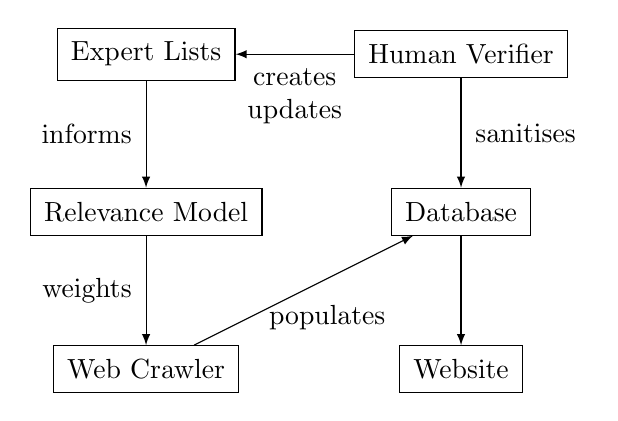
\begin{tikzpicture}[auto,on grid,>=latex,every node/.style={align=center,draw,rectangle,inner sep =5pt}]
\node (vocab) at (0,0) {Expert Lists};
\node (model) at (0,-2) {Relevance Model};
\node (crawl) at (0,-4) {Web Crawler};
\node (verify) at (4,0) {Human Verifier};
\node (db) at (4,-2) {Database};
\node (web) at (4,-4) {Website};

\draw[->] (vocab) edge node [draw = none,left] {informs} (model)
            (model) edge node [draw = none,left] {weights} (crawl)
            (crawl) edge node [draw = none,below,xshift=3mm] {populates} (db)
            (verify) edge node [draw = none] {sanitises} (db)
                edge node [draw = none] {creates\\updates} (vocab)
            (db) edge (web);

\end{tikzpicture}
\caption{All stages creating the resource.}
\label{fig:stages}
\end{center}
\end{figure}

\subsection{The Role of Human Verifiers}
\label{sec:verif}
The experts are involved in the resource creation workflow in two crucial steps.
Firstly, they are involved in creating the expert vocabulary/list with is used to inform the web crawler, and part of the initial sanitisation of items in the database.
Second, the experts routinely need to check any changes in the data from the web crawler to identify if the data is compromised.

Identifying potential Domestic Abuse services and determining what should be included in a comprehensive directory is difficult for non-expert humans. 
For example, some organizations offer support that may cater to people with historical abuse (i.e., those who have suffered abuse but are not currently fleeing from it; e.g., The Haven Project\cite{haven}), but they are not themselves Domestic Abuse services.
Further, some commercial entities may have special offers for Domestic Abuse survivors (e.g., financial abuse support through the Bank Of Scotland, pro Bono legal work through private law firms, etc.), but these usually require referral through recognized or affiliated Domestic Abuse services, and thus are not the priority for a survivor-facing database \cite{enduser}.  
Moreover, many local council websites provide information on Domestic Abuse alongside a phone number, but it can be extremely difficult to determine if the phone number is associated with a one-off Domestic Abuse service or just a general inquiry line that will signpost to specific Domestic Abuse services. To illustrate this point, see the Thanet Council webpage on Domestic Abuse ( \url{https://daris.wp.st-andrews.ac.uk/}). They provide a phone number to call in case of Domestic Abuse, heavily implying that they offer a one-off service. However, careful vetting of the phone number and associated project reveals that survivors are being referred to a homelessness service, not a domestic abuse service. This example shows precisely how important it is to develop a clear and simple database of relevant services for end users. It also demonstrates the necessity of (expert) human verification within the workflow.
These and other practical decisions based on the needs of the end user make it essential to include experts in the design and verification process. 
In our case, we must identify and include only programs from organizations specializing in Domestic Abuse response and prevention.

The list of terminology and vocabulary, as well as their importance for a sensitive topic like ``UK Domestic Abuse Services" must be created and configured by an expert.
There are too few UK services for a machine learning binary-classifier model to train on and they are hard to identify manually. 
The Women's Aid Directory numbers just 510 services.
Damm \& Kane \cite{dammkane2021} achieved a maximum of 57\% accuracy in labelling registered UK charities across various machine learning models, with a substantially larger dataset (6,203 labelled charities) than is achievable in our domain---though this was a multi-label classifier. 
While Ma \cite{ma2020} achieved 90\% accuracy in multi-class classification, that is also with a large dataset of US nonprofit organisations and significantly more complex model. 
Crucially, our use case requires a degree of human judgement that, as discussed, is challenging for non-experts.

A manually informed approach is thus more appropriate, and allows for the flexibility in the framework that we are aiming to achieve.
That means that we use the list of vocabulary and the knowledge of DARIS experts to infer weighted \textit{predicates} that can collectively identify domestic abuse services. 
We iteratively modified the predicates until the resulting provisional catalogue of webpages contains an amount of pages which is reasonable to ask an expert to review.

Once the initial catalogue is labelled, continuing to run the crawler should only generate trivially small increments to the dataset as services appear or disappear.
There is only a one-off large  manual cost, that is reviewing the initial catalogue. 
Results must nonetheless be manually reviewed before they are published to end users---importantly, our system facilitates both reviewing and updating the catalogue with a trivial manual burden in comparison with current fully manual efforts.



\subsection{List of Vocabulary and Features}
\label{sec:vocab}
A list of terms and expressions is curated by experts in the field who have researched the topic and service providers with practical knowledge. 
As mentioned, we specifically used DARIS and their community contacts in the present project\cite{theme}. 
This list needs to be constantly updated by the experts as the language around domestic abuse is fast evolving, which includes not only the addition of new terminology but also the change in the meaning of older, as well as long-standing terminology turning obsolete or even inappropriate (e.g., ``domestic abuse" vs. ``domestic violence", where the latter is appropriate in England but not Scotland).

Each of the phrases is assigned a relative weight, which we formalise in \cref{relmod}. For now, note that the weighting is determined by DARIS experts based on knowledge of what words or phrases strongly indicate that a given page represents a domestic abuse service in the region we are tackling.

In addition to vocabulary keywords, we look for particular features associated with domestic abuse services. 
The most notable are ``Quick Exit'' buttons: interactive elements that commonly appear on webpages servicing victims of domestic abuse, particularly those needing to hide their browsing activity from their abuser. 
As \cref{fig:exit} shows, they are not standardised with respect to design and wording.
We look for clickable HTML elements labelled by a word such as ``leave", ``exit", etc., along with either a mention of ``page", ``website", etc. \textit{or} ``quick", ``now", and so on (or both). In rare cases, the quick exit button will not explicitly contain text but rather an image or symbol, making it undetectable. Similarly, there are some one-off particular phrases used that are undetectable, but they are too infrequent to warrant the creation of a more complex model (for one, see Cornwall Refuge Trust in \cref{fig:exit}).

Another feature are charity codes. Registers of Scottish and rest-of-the-UK (rUK) charity codes are published by the Scottish Charity Regulator (OSCR), Charity Commission for England and Wales and Charity Commission for Northern Ireland \cite{scotchar, rukchar, nichar}.
Scottish charity codes are particularly useful because they are prefixed with ``SC". 
Conversely, rUK charity codes are 6 or 7 digit integers and---critically---sequential. 
Whenever we see a six or seven digit number, it is bound to correspond to \textit{some} charity irrespective of whether it actually represents one.

\begin{figure}
    \centering
    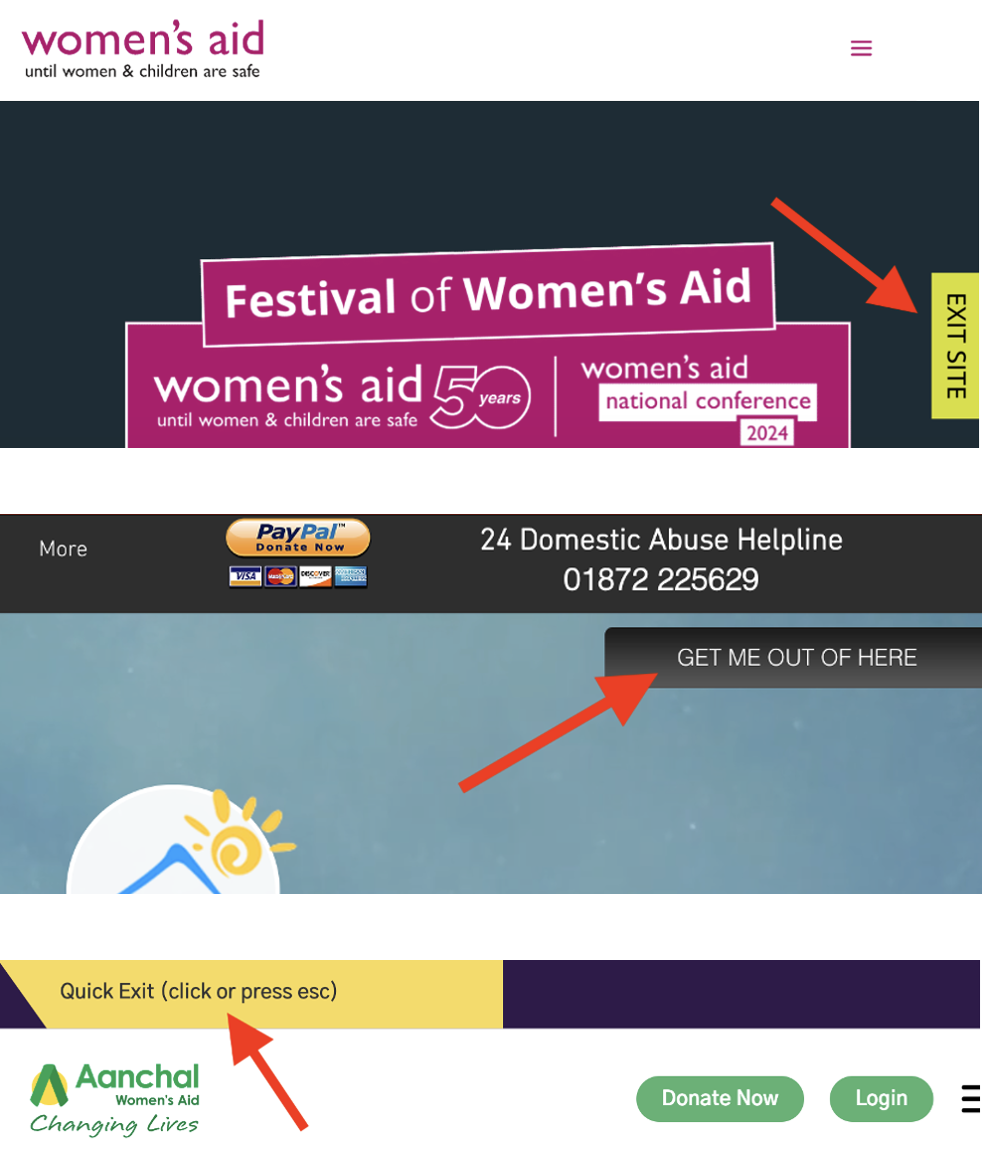
\includegraphics[width=1\linewidth]{quick-exit.png}
    \caption{Different Quick Exit buttons for Aanchal \cite{aanchalwa}, Cornwall Refuge Trust\cite{cornrt} and Women's Aid UK \cite{wauk}, respectively.}
    \label{fig:exit}
\end{figure}

The list of vocabulary/terminology can be replaced with another to create a resource for other sectors (e.g., services for people experiencing homelessness, services for recent immigrants/refugees, etc.). 
But as discussed above, should the list be adapted, experts need to be consulted about the importance of terms and checks of the web crawler's initial results must be performed to ascertain performance and make modifications as need be. 

\subsection{Relevance Modelling}
\label{relmod}

Relevance modelling incorporates the list of vocabulary and features and serves two purposes to our workflow. First, it allows us to decide whether to \textit{itemise} a page, i.e., add it to the database. Second, it allows us to prioritise URLs that are more likely to link to relevant pages.

As such, there are two models involved in ranking webpages for their relevance. 
Both share the same underlying mathematical functions, but the \textit{link model} investigates URLs, while the \textit{page model} evaluated the HTML content of the pages. We will first discuss the mathematical foundations (which both models share), before delving into its impact on the two models.

A set of predicates is initially derived from the list of vocabulary and features. Each item in the list is translated either as a regular expression predicate (e.g. matching the \url{.org.uk} top-level domain), an HTML lookup predicate (e.g. ``Quick Exit" buttons), or a keyword lookup predicate (e.g. the phrase ``intimate partner violence"). In particular, a keyword lookup predicate is a set of keyword sets along with an integer $n$, requiring $n$ terms of each keyword set to decide that the predicate is a match. For instance, to decide that a page is a news site we need both news-related terminology (e.g. ``news", ``headline") and enough general news topics to appear (e.g. ``politics", ``weather") --- ensuring that the page is news-related, as well that it is not, e.g., a ``news and announcements" section of a Domestic Abuse service website.

For each predicate $p$ from our list of vocabulary we manually assigned two weights $c_p$ and $s_p$, a \textit{constant} and a \textit{scaling} weight respectively. As described in \cref{sec:vocab}, these values are based on expert judgement. We also use successive crawls search for their optimal values. For example, the scaling effect of a Scottish charity code was initially set to relatively high value. Manually inspecting the predicates matched by false-positive pages revealed that this amplified charities that \textit{funded} domestic abuse services rather than \textit{ran} them. A reduced value thus reflected that Scottish charity status is a less reliable predictor of relevance than originally thought.

For an input $I$ (either an URL or the HTML content), and a set of predicates $P$ (the list of vocabulary and features), we calculate a score (which will lay in the interval $(-1,1)$) of the input as a logistical scale of the effects of the predicates' weights. Scores near -1 will indicate the overwhelming presence of predicates with negative effect, indicating irrelevance, while scores near 1 will indicate the overwhelming presence of positively weighted predicates, indicating relevance.

\begin{equation}
\begin{aligned}
\text{Score}(I, P) = & \sigma_{x_{90}}(\text{Compound}(I, P) \\ 
& +\gamma\text{WordCount}(I))
\end{aligned}
\label{eq:score}
\end{equation}

where $x_{90}$ is the $x$-value needed for the 90th percentile of positive confidence and $\gamma$ is a non-positive word count factor, both derived through an initial judgement and iteration.
We define  $\sigma_{x_{90}}: \mathbb{R}\rightarrow (-1,1)$ to be the transformation of the standard logistic function that passes through $(0, 0)$ and the point $(x_{90}, 0.90)$ with a supremum of 1.

The WordCount function counts how many words the input consists of. For a URL this will be 0, and for a page we remove markup elements such as HTML before counting.

The Compound function computes the cumulative effect of the constant and scaling factors of the matched predicates. So, for an input $I$ and a set of predicates $P$ it is 
\begin{equation}
\begin{aligned}
\text{Compound}(I, P) = & \left(\prod_{p\in P} s_p \text{ IsMatch}(I, p)\right) \\
& \times \left( \sum_{p\in P}c_p\text{ IsMatch}(I, p)\right)
\end{aligned}
\label{eq:comp}
\end{equation}

where IsMatch is a boolean function; if part of the input $I$ matches the predicate $p$ then we assign it the value $1$.

Because Score is continuous (rather than, e.g., classifying 0/1 for relevant/irrelevant), it can be used in combination with \textit{meta-heuristics} to make a final decision on relevance. As will be discussed further, we may be confident that a particular website is relevant if it is dense in reasonably high-scoring pages even if no individual page has an exceptional score (some services' pages can be relatively bare). A binary judgement of 0/1 by the scorer would not allow this flexibility on the part of the crawler.

The link model generates an \textit{lscore} (based on \cref{eq:score}) between -1 and 1 that indicates relevance to the ``broad topic" of our search: UK-based services, charities and organisations. 
The reason for the link model being ``broad" is that URL text is not enough information to classify the page it links to. 
We may be able to infer, for instance, that a given link refers to a British charity if it ends in \texttt{.org.uk} and matches the vocabulary words ``charity" and ``foundation"---but it is impossible to infer \textit{what} the charity is about, and our manual inspection of known domestic abuse services indicated that URLs do not consistently offer such granular insight.

This also means links are rarely penalised: URLs simply do not provide enough hints to confidently do so. Therefore, lscore does not implement negative predicates, with the exception of regional TLDs of non-UK Enlish-speaking nations, which are weighted as $-\infty$ to avoid visiting altogether. Negative lscores are thus rare.

The page model predicts whether a given page is a domestic abuse service; that is the \textit{pscore} of the page (again based on \cref{eq:score}). 
A pscore ranges between -1 and 1, where 1 indicates absolute certainty that the page is relevant and -1 that it is irrelevant.

\textbf{this is how far I got $\leftarrow$ RUTH, but having a quick scan over some of the below, could this be the weighting thing that I was hoping to have covered in a previous section? If so, SHIFT IT :D}

Scaling and constant terms accumulate separately such that their effect is independent of the order in which they are matched. Crucially, scaling terms enable us to approximate a contextual understanding of different terms in the text---essentially, depending on its $s$-weight, a predicate can have a dampening or a amplifying effect on other predicates. For example, the predicate matching universities and academic journals was ultimately set a 0.7 scaling weight, dampening the effect of the keyphrase ``coercive control" by 30\% as informed by the fact that the mention is likely in an academic context. Conversely, matching a Scottish charity code has a 1.2 scaling weight, as it reveals that the page is contextually relevant.

A word-count factor is needed because wordy pages (e.g. ``Terms and Conditions" documents) tend to match more predicates irrespective of whether they are relevant overall. One approach is to divide the compounded weights by the word count and consider the predicate \textit{density} of a page. However, we found this approach to unnecessarily penalise some relevant websites; for instance, larger services may focus on more topics than domestic abuse, making their pages sparser in relevant keywords. A constant word-count factor avoids over-penalising relevant pages, while filtering out those who are so unusually wordy that they may match keyword predicates solely by chance.

In summary, \textit{pscore} is composed of predicates for the following:
\begin{itemize}
    \item Keyword and keyphrase matches.
    \item Presence of a ``Quick Exit" element.
    \item Scottish charity codes.
\end{itemize}

\textit{lscore} similarly considers:
\begin{itemize}
    \item Keyword matches.
    \item Top-Level Domains (TLDs), e.g. org.uk.
    \item pscore of the \textit{parent page}, that is the page from which the link was obtained.
\end{itemize}

So far, we have discussed how we score pages on the likelihood that they service domestic abuse victims. However, we must also ensure that the domestic abuse services we identify are UK-based. A way of doing this would be to develop a set of ``localisation" predicates for pscore. For instance, we could match regional linguistic hints such as spellings or idioms, place names and phone numbers in conjunction with \textit{whois} lookups. But a naive implementation of such a mechanism is bound to be inaccurate: spelling variants and place names are often duplicated across English-speaking nations (especially in the Commonwealth) and \textit{whois} can be anonymised (as it often is by services that are naturally concerned with privacy). As an aside, it would be more difficult to look for services in Scotland rather than UK-wide precisely because it would require our localisation mechanism to be more granular. We aim to develop a more sophisticated localisation mechanism as future work for labelling the discovered services, in order that they may be recommended to end users depending on their region.

For the scope of this paper, instead of trying to accurately classify pages by country, we limit our search space to links that are likely to be associated with the UK. We found success in using lscore as our localisation mechanism. In effect, we:
\begin{itemize}
    \item Dampen links with TLDs belonging to other English-speaking countries, such as .gov, .edu, .ie, .au, etc.
    \item Implicitly boost links discovered in websites with OSCR codes, through the ``parent pscore" heuristic.
    \item Initially populate the search space with known UK-based organisations.
\end{itemize}

\subsection{Web Crawler}
\label{sec:crawl}

The web crawler begins a search from a set of 212 pages that belong to prominent UK-based domestic abuse services. Each of the starting pages has a priority of $+\infty$. When a website is visited, all links from it are extracted and added to the visit frontier with priority ratings on a discrete 20-rank scale according to their lscore.

An in-memory cache of the pscores for every First-Level Domain (FLD, used here to mean its domain followed by the TLD) is maintained. If upon visiting a page we score it above a given ``exceptional" threshold, the page is itemised. Otherwise, we look at the cached pscores for the given FLD. If there are enough samples, and the proportion of pages having a ``good" pscore is high, we itemise the FLD. We have found 0.95, 0.80 and 60\% to be appropriate ``exceptional", ``good" and ``proportion of `good' pages" thresholds, but this will likely vary by topic, predicates and the desired accuracy/recall trade-off. Lower thresholds will generate more itemisations. In our case, we sought a middle ground between recall and accuracy; we can manually filter out some irrelevant results, but our aim is also to reduce the manual burden of manually discovering services. We iteratively tested short crawls with different thresholds, sampled their results and adjusted as needed.

This iteration also allowed us to explicitly handle some edge cases, namely:
\begin{itemize}
    \item Some news sites and political advocacy groups include wording that is hard to differentiate from, e.g., larger Domestic Abuse services with a ``news" section to their website.
    \item UK government data sources publish documents addressing Domestic Abuse that are dense in relevant terminology \textit{and} come from a .gov.uk source.
    \item One-time events (e.g. training or awareness seminars) that are dense in relevant text appear on ticket-booking websites.
\end{itemize}

We explicitly blacklist these websites. Modifying the page model to exclude them would likely overfit it to these particular cases.

A significant challenge in crawling is identifying \textit{crawler traps}, that is websites that generate infinitely many discovered links for a crawler to visit. Calendars are a classic example: each calendar page may contain a distinct link to the page chronologically succeeding it, thereby creating an inexhaustible source of links. Our link prioritisation mechanism exacerbates this risk, as a crawler trap with high-ranking links could endlessly dominate the search. We safeguard against crawler traps by only visiting each page once (hence avoiding loops) and bounding above the number of requests the crawler may make to a single FLD.

Other badly behaved websites can cause our requests to repeatedly fail or time out. We thus also bound above the number of failed requests we allow for any website. Of course, we expect \textit{some} bad responses, e.g. due to outdated links.

Legitimate Scottish resources have to carry the Scottish Charity number of on the page, which we can filter for as well.

As an aside, the crawling phase of the resource could look through OSCR only. 
The OSCR keeps records about the registered charities in Scotland, these include location, whether the charity is active and some details about the charity. 
We have found that the OSCR does not contain enough information about the domestic abuse charities for us to be able to identify which services they might provide and for whom.
But we are using this register to verify the crawled websites as well as sanitise the data set.

Owing to link prioritisation, we expect that the rate of discovery of relevant websites (i.e. \# Unseen FLDs found to be relevant / Requests made) generally diminishes as more pages are visited. It is nonetheless difficult to know for certain when to stop the crawl. While results may become irrelevant for some time during the crawl, there is a likelihood that a cluster of relevant, unseen pages will soon be discovered. For this reason, we run the crawl for longer than we anticipate will yield relevant pages. Ensuing analysis of the results will reveal from which point onwards they are too often irrelevant for us to extend the crawl.

This is useful knowledge for subsequent crawls, which will be used to update the initial catalogue. Running a crawl for the number of pages visited during the initial one, we will notice that some services have disappeared (due to disappearing services' websites no longer being hosted or links to them being removed) and that new ones have appeared. These discrepancies will then be manually reviewed and integrated to our catalogue.

Any new FLDs that are confirmed to be relevant will also be added to the set of starting pages for subsequent crawls. Increasing the number of known relevant starting pages for the crawl will likely increase the chance that an unseen relevant result will be detected early. That is because links to relevant pages will normally be found no more than a few links' distance from some other relevant page. Considering that one service need not directly link to another for this to be true (e.g. it could link to the website of a local council, which provides a directory of local Domestic Abuse services) it is highly unlikely that some valid service would not be linked to in this manner. Confirming this empirically over several crawls will be allow a gradual decrease in the length of each subsequent crawl.

The crawler is implemented in Scrapy 2.11 \cite{scrapy}, an established, well-documented crawling framework for Python. We output the live crawl results to a PostgreSQL database export as CSV the results of queries that require expert review.

\section{Results of the Initial Crawl}
\label{sec:res}

Using ``eyeball" estimates of the results of earlier crawls, it is possible to make a liberal estimate of how long to run the initial crawl for.
For the particular crawler configuration and the search topic that this paper covers, 2,000 domains would be sufficient to exhaust the parts of the search space that could yield relevant results.
Effectively, we can be reasonably confident that there are very few clusters of websites that are relevant but so far unvisited. 

More importantly, if there are few undiscovered relevant results, the rate at which we discover them (\# relevant domains visited / \# all domains visited) necessarily decreases, and therefore the rate of false positives rises.
As such, the database will contain a greater proportion of irrelevant results for a human expert to filter out, implying rapidly diminishing marginal returns once most relevant domains are itemised.
The cost of an overlong crawl is not measured only in machine time, but also human time.

The initial crawl itemised 2,162 different domains. Of those, we randomly sampled 300 and shuffled them for two independent coders to review.

Each coder marked three boolean flags for each domain in the subsample:

\begin{enumerate}
    \item \textbf{Relevant}. The organisation offers support directly to Domestic Abuse survivors and provide services related to one of the following:
        \begin{itemize}
            \item Domestic abuse (including all forms of abuse that occur in the home/in a relationship, such as partner abuse, child abuse, parent abuse, abuse of a pet, physical, emotional, sexual, financial, etc.)
            \item Sexual violence (in or outside of the home) 
            \item Human trafficking 
            \item Forced marriage/child marriage 
            \item Youth centre (with at least one Domestic Abuse service) 
        \end{itemize}
    \item \textbf{Specialised}. The organisation does not just provide a ``one-off" service, that is a service on the list above, while otherwise \textit{not} being an organisation of the nature listed above.
    \item \textbf{Active in the UK}. The organisation offers support directly to survivors in the UK.
\end{enumerate}

Note that the 2,162 visited pages are not a representative sample of the general web, so the results of this coding do not generalise to the performance of the page relevance model.
First, the prioritisation mechanism and identification of starting pages biases it in favour of likely relevant pages.
Secondly, the choice of cut-off point to end the crawl affects the proportion of false positives in the result set, for the reasons discussed earlier.

\begin{figure}
    \centering
    \resizebox{8cm}{!}{%% Creator: Matplotlib, PGF backend
%%
%% To include the figure in your LaTeX document, write
%%   \input{<filename>.pgf}
%%
%% Make sure the required packages are loaded in your preamble
%%   \usepackage{pgf}
%%
%% Also ensure that all the required font packages are loaded; for instance,
%% the lmodern package is sometimes necessary when using math font.
%%   \usepackage{lmodern}
%%
%% Figures using additional raster images can only be included by \input if
%% they are in the same directory as the main LaTeX file. For loading figures
%% from other directories you can use the `import` package
%%   \usepackage{import}
%%
%% and then include the figures with
%%   \import{<path to file>}{<filename>.pgf}
%%
%% Matplotlib used the following preamble
%%   \def\mathdefault#1{#1}
%%   \everymath=\expandafter{\the\everymath\displaystyle}
%%   
%%   \usepackage{fontspec}
%%   \setmainfont{DejaVuSerif.ttf}[Path=\detokenize{/opt/homebrew/lib/python3.11/site-packages/matplotlib/mpl-data/fonts/ttf/}]
%%   \setsansfont{DejaVuSans.ttf}[Path=\detokenize{/opt/homebrew/lib/python3.11/site-packages/matplotlib/mpl-data/fonts/ttf/}]
%%   \setmonofont{DejaVuSansMono.ttf}[Path=\detokenize{/opt/homebrew/lib/python3.11/site-packages/matplotlib/mpl-data/fonts/ttf/}]
%%   \makeatletter\@ifpackageloaded{underscore}{}{\usepackage[strings]{underscore}}\makeatother
%%
\begingroup%
\makeatletter%
\begin{pgfpicture}%
\pgfpathrectangle{\pgfpointorigin}{\pgfqpoint{6.400000in}{4.800000in}}%
\pgfusepath{use as bounding box, clip}%
\begin{pgfscope}%
\pgfsetbuttcap%
\pgfsetmiterjoin%
\definecolor{currentfill}{rgb}{1.000000,1.000000,1.000000}%
\pgfsetfillcolor{currentfill}%
\pgfsetlinewidth{0.000000pt}%
\definecolor{currentstroke}{rgb}{1.000000,1.000000,1.000000}%
\pgfsetstrokecolor{currentstroke}%
\pgfsetdash{}{0pt}%
\pgfpathmoveto{\pgfqpoint{0.000000in}{0.000000in}}%
\pgfpathlineto{\pgfqpoint{6.400000in}{0.000000in}}%
\pgfpathlineto{\pgfqpoint{6.400000in}{4.800000in}}%
\pgfpathlineto{\pgfqpoint{0.000000in}{4.800000in}}%
\pgfpathlineto{\pgfqpoint{0.000000in}{0.000000in}}%
\pgfpathclose%
\pgfusepath{fill}%
\end{pgfscope}%
\begin{pgfscope}%
\pgfsetbuttcap%
\pgfsetmiterjoin%
\definecolor{currentfill}{rgb}{1.000000,1.000000,1.000000}%
\pgfsetfillcolor{currentfill}%
\pgfsetlinewidth{0.000000pt}%
\definecolor{currentstroke}{rgb}{0.000000,0.000000,0.000000}%
\pgfsetstrokecolor{currentstroke}%
\pgfsetstrokeopacity{0.000000}%
\pgfsetdash{}{0pt}%
\pgfpathmoveto{\pgfqpoint{0.708403in}{0.634956in}}%
\pgfpathlineto{\pgfqpoint{6.250000in}{0.634956in}}%
\pgfpathlineto{\pgfqpoint{6.250000in}{4.436667in}}%
\pgfpathlineto{\pgfqpoint{0.708403in}{4.436667in}}%
\pgfpathlineto{\pgfqpoint{0.708403in}{0.634956in}}%
\pgfpathclose%
\pgfusepath{fill}%
\end{pgfscope}%
\begin{pgfscope}%
\pgfpathrectangle{\pgfqpoint{0.708403in}{0.634956in}}{\pgfqpoint{5.541597in}{3.801711in}}%
\pgfusepath{clip}%
\pgfsetbuttcap%
\pgfsetmiterjoin%
\definecolor{currentfill}{rgb}{0.000000,0.419608,0.643137}%
\pgfsetfillcolor{currentfill}%
\pgfsetlinewidth{0.000000pt}%
\definecolor{currentstroke}{rgb}{0.000000,0.000000,0.000000}%
\pgfsetstrokecolor{currentstroke}%
\pgfsetstrokeopacity{0.000000}%
\pgfsetdash{}{0pt}%
\pgfpathmoveto{\pgfqpoint{1.678182in}{0.634956in}}%
\pgfpathlineto{\pgfqpoint{2.509422in}{0.634956in}}%
\pgfpathlineto{\pgfqpoint{2.509422in}{2.703086in}}%
\pgfpathlineto{\pgfqpoint{1.678182in}{2.703086in}}%
\pgfpathlineto{\pgfqpoint{1.678182in}{0.634956in}}%
\pgfpathclose%
\pgfusepath{fill}%
\end{pgfscope}%
\begin{pgfscope}%
\pgfpathrectangle{\pgfqpoint{0.708403in}{0.634956in}}{\pgfqpoint{5.541597in}{3.801711in}}%
\pgfusepath{clip}%
\pgfsetbuttcap%
\pgfsetmiterjoin%
\definecolor{currentfill}{rgb}{0.000000,0.419608,0.643137}%
\pgfsetfillcolor{currentfill}%
\pgfsetlinewidth{0.000000pt}%
\definecolor{currentstroke}{rgb}{0.000000,0.000000,0.000000}%
\pgfsetstrokecolor{currentstroke}%
\pgfsetstrokeopacity{0.000000}%
\pgfsetdash{}{0pt}%
\pgfpathmoveto{\pgfqpoint{4.448981in}{0.634956in}}%
\pgfpathlineto{\pgfqpoint{5.280220in}{0.634956in}}%
\pgfpathlineto{\pgfqpoint{5.280220in}{2.064399in}}%
\pgfpathlineto{\pgfqpoint{4.448981in}{2.064399in}}%
\pgfpathlineto{\pgfqpoint{4.448981in}{0.634956in}}%
\pgfpathclose%
\pgfusepath{fill}%
\end{pgfscope}%
\begin{pgfscope}%
\pgfpathrectangle{\pgfqpoint{0.708403in}{0.634956in}}{\pgfqpoint{5.541597in}{3.801711in}}%
\pgfusepath{clip}%
\pgfsetbuttcap%
\pgfsetmiterjoin%
\definecolor{currentfill}{rgb}{1.000000,0.501961,0.054902}%
\pgfsetfillcolor{currentfill}%
\pgfsetlinewidth{0.000000pt}%
\definecolor{currentstroke}{rgb}{0.000000,0.000000,0.000000}%
\pgfsetstrokecolor{currentstroke}%
\pgfsetstrokeopacity{0.000000}%
\pgfsetdash{}{0pt}%
\pgfpathmoveto{\pgfqpoint{1.678182in}{2.703086in}}%
\pgfpathlineto{\pgfqpoint{2.509422in}{2.703086in}}%
\pgfpathlineto{\pgfqpoint{2.509422in}{3.280946in}}%
\pgfpathlineto{\pgfqpoint{1.678182in}{3.280946in}}%
\pgfpathlineto{\pgfqpoint{1.678182in}{2.703086in}}%
\pgfpathclose%
\pgfusepath{fill}%
\end{pgfscope}%
\begin{pgfscope}%
\pgfpathrectangle{\pgfqpoint{0.708403in}{0.634956in}}{\pgfqpoint{5.541597in}{3.801711in}}%
\pgfusepath{clip}%
\pgfsetbuttcap%
\pgfsetmiterjoin%
\definecolor{currentfill}{rgb}{1.000000,0.501961,0.054902}%
\pgfsetfillcolor{currentfill}%
\pgfsetlinewidth{0.000000pt}%
\definecolor{currentstroke}{rgb}{0.000000,0.000000,0.000000}%
\pgfsetstrokecolor{currentstroke}%
\pgfsetstrokeopacity{0.000000}%
\pgfsetdash{}{0pt}%
\pgfpathmoveto{\pgfqpoint{4.448981in}{2.064399in}}%
\pgfpathlineto{\pgfqpoint{5.280220in}{2.064399in}}%
\pgfpathlineto{\pgfqpoint{5.280220in}{3.098464in}}%
\pgfpathlineto{\pgfqpoint{4.448981in}{3.098464in}}%
\pgfpathlineto{\pgfqpoint{4.448981in}{2.064399in}}%
\pgfpathclose%
\pgfusepath{fill}%
\end{pgfscope}%
\begin{pgfscope}%
\pgfpathrectangle{\pgfqpoint{0.708403in}{0.634956in}}{\pgfqpoint{5.541597in}{3.801711in}}%
\pgfusepath{clip}%
\pgfsetbuttcap%
\pgfsetmiterjoin%
\definecolor{currentfill}{rgb}{0.670588,0.670588,0.670588}%
\pgfsetfillcolor{currentfill}%
\pgfsetlinewidth{0.000000pt}%
\definecolor{currentstroke}{rgb}{0.000000,0.000000,0.000000}%
\pgfsetstrokecolor{currentstroke}%
\pgfsetstrokeopacity{0.000000}%
\pgfsetdash{}{0pt}%
\pgfpathmoveto{\pgfqpoint{1.678182in}{3.280946in}}%
\pgfpathlineto{\pgfqpoint{2.509422in}{3.280946in}}%
\pgfpathlineto{\pgfqpoint{2.509422in}{4.254185in}}%
\pgfpathlineto{\pgfqpoint{1.678182in}{4.254185in}}%
\pgfpathlineto{\pgfqpoint{1.678182in}{3.280946in}}%
\pgfpathclose%
\pgfusepath{fill}%
\end{pgfscope}%
\begin{pgfscope}%
\pgfpathrectangle{\pgfqpoint{0.708403in}{0.634956in}}{\pgfqpoint{5.541597in}{3.801711in}}%
\pgfusepath{clip}%
\pgfsetbuttcap%
\pgfsetmiterjoin%
\definecolor{currentfill}{rgb}{0.670588,0.670588,0.670588}%
\pgfsetfillcolor{currentfill}%
\pgfsetlinewidth{0.000000pt}%
\definecolor{currentstroke}{rgb}{0.000000,0.000000,0.000000}%
\pgfsetstrokecolor{currentstroke}%
\pgfsetstrokeopacity{0.000000}%
\pgfsetdash{}{0pt}%
\pgfpathmoveto{\pgfqpoint{4.448981in}{3.098464in}}%
\pgfpathlineto{\pgfqpoint{5.280220in}{3.098464in}}%
\pgfpathlineto{\pgfqpoint{5.280220in}{3.980461in}}%
\pgfpathlineto{\pgfqpoint{4.448981in}{3.980461in}}%
\pgfpathlineto{\pgfqpoint{4.448981in}{3.098464in}}%
\pgfpathclose%
\pgfusepath{fill}%
\end{pgfscope}%
\begin{pgfscope}%
\pgfsetbuttcap%
\pgfsetroundjoin%
\definecolor{currentfill}{rgb}{0.000000,0.000000,0.000000}%
\pgfsetfillcolor{currentfill}%
\pgfsetlinewidth{0.803000pt}%
\definecolor{currentstroke}{rgb}{0.000000,0.000000,0.000000}%
\pgfsetstrokecolor{currentstroke}%
\pgfsetdash{}{0pt}%
\pgfsys@defobject{currentmarker}{\pgfqpoint{0.000000in}{-0.048611in}}{\pgfqpoint{0.000000in}{0.000000in}}{%
\pgfpathmoveto{\pgfqpoint{0.000000in}{0.000000in}}%
\pgfpathlineto{\pgfqpoint{0.000000in}{-0.048611in}}%
\pgfusepath{stroke,fill}%
}%
\begin{pgfscope}%
\pgfsys@transformshift{2.093802in}{0.634956in}%
\pgfsys@useobject{currentmarker}{}%
\end{pgfscope}%
\end{pgfscope}%
\begin{pgfscope}%
\definecolor{textcolor}{rgb}{0.000000,0.000000,0.000000}%
\pgfsetstrokecolor{textcolor}%
\pgfsetfillcolor{textcolor}%
\pgftext[x=2.093802in,y=0.537733in,,top]{\color{textcolor}{\sffamily\fontsize{10.000000}{12.000000}\selectfont\catcode`\^=\active\def^{\ifmmode\sp\else\^{}\fi}\catcode`\%=\active\def%{\%}Coder A}}%
\end{pgfscope}%
\begin{pgfscope}%
\pgfsetbuttcap%
\pgfsetroundjoin%
\definecolor{currentfill}{rgb}{0.000000,0.000000,0.000000}%
\pgfsetfillcolor{currentfill}%
\pgfsetlinewidth{0.803000pt}%
\definecolor{currentstroke}{rgb}{0.000000,0.000000,0.000000}%
\pgfsetstrokecolor{currentstroke}%
\pgfsetdash{}{0pt}%
\pgfsys@defobject{currentmarker}{\pgfqpoint{0.000000in}{-0.048611in}}{\pgfqpoint{0.000000in}{0.000000in}}{%
\pgfpathmoveto{\pgfqpoint{0.000000in}{0.000000in}}%
\pgfpathlineto{\pgfqpoint{0.000000in}{-0.048611in}}%
\pgfusepath{stroke,fill}%
}%
\begin{pgfscope}%
\pgfsys@transformshift{4.864601in}{0.634956in}%
\pgfsys@useobject{currentmarker}{}%
\end{pgfscope}%
\end{pgfscope}%
\begin{pgfscope}%
\definecolor{textcolor}{rgb}{0.000000,0.000000,0.000000}%
\pgfsetstrokecolor{textcolor}%
\pgfsetfillcolor{textcolor}%
\pgftext[x=4.864601in,y=0.537733in,,top]{\color{textcolor}{\sffamily\fontsize{10.000000}{12.000000}\selectfont\catcode`\^=\active\def^{\ifmmode\sp\else\^{}\fi}\catcode`\%=\active\def%{\%}Coder B}}%
\end{pgfscope}%
\begin{pgfscope}%
\pgfsetbuttcap%
\pgfsetroundjoin%
\definecolor{currentfill}{rgb}{0.000000,0.000000,0.000000}%
\pgfsetfillcolor{currentfill}%
\pgfsetlinewidth{0.803000pt}%
\definecolor{currentstroke}{rgb}{0.000000,0.000000,0.000000}%
\pgfsetstrokecolor{currentstroke}%
\pgfsetdash{}{0pt}%
\pgfsys@defobject{currentmarker}{\pgfqpoint{-0.048611in}{0.000000in}}{\pgfqpoint{-0.000000in}{0.000000in}}{%
\pgfpathmoveto{\pgfqpoint{-0.000000in}{0.000000in}}%
\pgfpathlineto{\pgfqpoint{-0.048611in}{0.000000in}}%
\pgfusepath{stroke,fill}%
}%
\begin{pgfscope}%
\pgfsys@transformshift{0.708403in}{0.634956in}%
\pgfsys@useobject{currentmarker}{}%
\end{pgfscope}%
\end{pgfscope}%
\begin{pgfscope}%
\definecolor{textcolor}{rgb}{0.000000,0.000000,0.000000}%
\pgfsetstrokecolor{textcolor}%
\pgfsetfillcolor{textcolor}%
\pgftext[x=0.522815in, y=0.582194in, left, base]{\color{textcolor}{\sffamily\fontsize{10.000000}{12.000000}\selectfont\catcode`\^=\active\def^{\ifmmode\sp\else\^{}\fi}\catcode`\%=\active\def%{\%}0}}%
\end{pgfscope}%
\begin{pgfscope}%
\pgfsetbuttcap%
\pgfsetroundjoin%
\definecolor{currentfill}{rgb}{0.000000,0.000000,0.000000}%
\pgfsetfillcolor{currentfill}%
\pgfsetlinewidth{0.803000pt}%
\definecolor{currentstroke}{rgb}{0.000000,0.000000,0.000000}%
\pgfsetstrokecolor{currentstroke}%
\pgfsetdash{}{0pt}%
\pgfsys@defobject{currentmarker}{\pgfqpoint{-0.048611in}{0.000000in}}{\pgfqpoint{-0.000000in}{0.000000in}}{%
\pgfpathmoveto{\pgfqpoint{-0.000000in}{0.000000in}}%
\pgfpathlineto{\pgfqpoint{-0.048611in}{0.000000in}}%
\pgfusepath{stroke,fill}%
}%
\begin{pgfscope}%
\pgfsys@transformshift{0.708403in}{1.243229in}%
\pgfsys@useobject{currentmarker}{}%
\end{pgfscope}%
\end{pgfscope}%
\begin{pgfscope}%
\definecolor{textcolor}{rgb}{0.000000,0.000000,0.000000}%
\pgfsetstrokecolor{textcolor}%
\pgfsetfillcolor{textcolor}%
\pgftext[x=0.434450in, y=1.190468in, left, base]{\color{textcolor}{\sffamily\fontsize{10.000000}{12.000000}\selectfont\catcode`\^=\active\def^{\ifmmode\sp\else\^{}\fi}\catcode`\%=\active\def%{\%}20}}%
\end{pgfscope}%
\begin{pgfscope}%
\pgfsetbuttcap%
\pgfsetroundjoin%
\definecolor{currentfill}{rgb}{0.000000,0.000000,0.000000}%
\pgfsetfillcolor{currentfill}%
\pgfsetlinewidth{0.803000pt}%
\definecolor{currentstroke}{rgb}{0.000000,0.000000,0.000000}%
\pgfsetstrokecolor{currentstroke}%
\pgfsetdash{}{0pt}%
\pgfsys@defobject{currentmarker}{\pgfqpoint{-0.048611in}{0.000000in}}{\pgfqpoint{-0.000000in}{0.000000in}}{%
\pgfpathmoveto{\pgfqpoint{-0.000000in}{0.000000in}}%
\pgfpathlineto{\pgfqpoint{-0.048611in}{0.000000in}}%
\pgfusepath{stroke,fill}%
}%
\begin{pgfscope}%
\pgfsys@transformshift{0.708403in}{1.851503in}%
\pgfsys@useobject{currentmarker}{}%
\end{pgfscope}%
\end{pgfscope}%
\begin{pgfscope}%
\definecolor{textcolor}{rgb}{0.000000,0.000000,0.000000}%
\pgfsetstrokecolor{textcolor}%
\pgfsetfillcolor{textcolor}%
\pgftext[x=0.434450in, y=1.798742in, left, base]{\color{textcolor}{\sffamily\fontsize{10.000000}{12.000000}\selectfont\catcode`\^=\active\def^{\ifmmode\sp\else\^{}\fi}\catcode`\%=\active\def%{\%}40}}%
\end{pgfscope}%
\begin{pgfscope}%
\pgfsetbuttcap%
\pgfsetroundjoin%
\definecolor{currentfill}{rgb}{0.000000,0.000000,0.000000}%
\pgfsetfillcolor{currentfill}%
\pgfsetlinewidth{0.803000pt}%
\definecolor{currentstroke}{rgb}{0.000000,0.000000,0.000000}%
\pgfsetstrokecolor{currentstroke}%
\pgfsetdash{}{0pt}%
\pgfsys@defobject{currentmarker}{\pgfqpoint{-0.048611in}{0.000000in}}{\pgfqpoint{-0.000000in}{0.000000in}}{%
\pgfpathmoveto{\pgfqpoint{-0.000000in}{0.000000in}}%
\pgfpathlineto{\pgfqpoint{-0.048611in}{0.000000in}}%
\pgfusepath{stroke,fill}%
}%
\begin{pgfscope}%
\pgfsys@transformshift{0.708403in}{2.459777in}%
\pgfsys@useobject{currentmarker}{}%
\end{pgfscope}%
\end{pgfscope}%
\begin{pgfscope}%
\definecolor{textcolor}{rgb}{0.000000,0.000000,0.000000}%
\pgfsetstrokecolor{textcolor}%
\pgfsetfillcolor{textcolor}%
\pgftext[x=0.434450in, y=2.407015in, left, base]{\color{textcolor}{\sffamily\fontsize{10.000000}{12.000000}\selectfont\catcode`\^=\active\def^{\ifmmode\sp\else\^{}\fi}\catcode`\%=\active\def%{\%}60}}%
\end{pgfscope}%
\begin{pgfscope}%
\pgfsetbuttcap%
\pgfsetroundjoin%
\definecolor{currentfill}{rgb}{0.000000,0.000000,0.000000}%
\pgfsetfillcolor{currentfill}%
\pgfsetlinewidth{0.803000pt}%
\definecolor{currentstroke}{rgb}{0.000000,0.000000,0.000000}%
\pgfsetstrokecolor{currentstroke}%
\pgfsetdash{}{0pt}%
\pgfsys@defobject{currentmarker}{\pgfqpoint{-0.048611in}{0.000000in}}{\pgfqpoint{-0.000000in}{0.000000in}}{%
\pgfpathmoveto{\pgfqpoint{-0.000000in}{0.000000in}}%
\pgfpathlineto{\pgfqpoint{-0.048611in}{0.000000in}}%
\pgfusepath{stroke,fill}%
}%
\begin{pgfscope}%
\pgfsys@transformshift{0.708403in}{3.068051in}%
\pgfsys@useobject{currentmarker}{}%
\end{pgfscope}%
\end{pgfscope}%
\begin{pgfscope}%
\definecolor{textcolor}{rgb}{0.000000,0.000000,0.000000}%
\pgfsetstrokecolor{textcolor}%
\pgfsetfillcolor{textcolor}%
\pgftext[x=0.434450in, y=3.015289in, left, base]{\color{textcolor}{\sffamily\fontsize{10.000000}{12.000000}\selectfont\catcode`\^=\active\def^{\ifmmode\sp\else\^{}\fi}\catcode`\%=\active\def%{\%}80}}%
\end{pgfscope}%
\begin{pgfscope}%
\pgfsetbuttcap%
\pgfsetroundjoin%
\definecolor{currentfill}{rgb}{0.000000,0.000000,0.000000}%
\pgfsetfillcolor{currentfill}%
\pgfsetlinewidth{0.803000pt}%
\definecolor{currentstroke}{rgb}{0.000000,0.000000,0.000000}%
\pgfsetstrokecolor{currentstroke}%
\pgfsetdash{}{0pt}%
\pgfsys@defobject{currentmarker}{\pgfqpoint{-0.048611in}{0.000000in}}{\pgfqpoint{-0.000000in}{0.000000in}}{%
\pgfpathmoveto{\pgfqpoint{-0.000000in}{0.000000in}}%
\pgfpathlineto{\pgfqpoint{-0.048611in}{0.000000in}}%
\pgfusepath{stroke,fill}%
}%
\begin{pgfscope}%
\pgfsys@transformshift{0.708403in}{3.676324in}%
\pgfsys@useobject{currentmarker}{}%
\end{pgfscope}%
\end{pgfscope}%
\begin{pgfscope}%
\definecolor{textcolor}{rgb}{0.000000,0.000000,0.000000}%
\pgfsetstrokecolor{textcolor}%
\pgfsetfillcolor{textcolor}%
\pgftext[x=0.346085in, y=3.623563in, left, base]{\color{textcolor}{\sffamily\fontsize{10.000000}{12.000000}\selectfont\catcode`\^=\active\def^{\ifmmode\sp\else\^{}\fi}\catcode`\%=\active\def%{\%}100}}%
\end{pgfscope}%
\begin{pgfscope}%
\pgfsetbuttcap%
\pgfsetroundjoin%
\definecolor{currentfill}{rgb}{0.000000,0.000000,0.000000}%
\pgfsetfillcolor{currentfill}%
\pgfsetlinewidth{0.803000pt}%
\definecolor{currentstroke}{rgb}{0.000000,0.000000,0.000000}%
\pgfsetstrokecolor{currentstroke}%
\pgfsetdash{}{0pt}%
\pgfsys@defobject{currentmarker}{\pgfqpoint{-0.048611in}{0.000000in}}{\pgfqpoint{-0.000000in}{0.000000in}}{%
\pgfpathmoveto{\pgfqpoint{-0.000000in}{0.000000in}}%
\pgfpathlineto{\pgfqpoint{-0.048611in}{0.000000in}}%
\pgfusepath{stroke,fill}%
}%
\begin{pgfscope}%
\pgfsys@transformshift{0.708403in}{4.284598in}%
\pgfsys@useobject{currentmarker}{}%
\end{pgfscope}%
\end{pgfscope}%
\begin{pgfscope}%
\definecolor{textcolor}{rgb}{0.000000,0.000000,0.000000}%
\pgfsetstrokecolor{textcolor}%
\pgfsetfillcolor{textcolor}%
\pgftext[x=0.346085in, y=4.231837in, left, base]{\color{textcolor}{\sffamily\fontsize{10.000000}{12.000000}\selectfont\catcode`\^=\active\def^{\ifmmode\sp\else\^{}\fi}\catcode`\%=\active\def%{\%}120}}%
\end{pgfscope}%
\begin{pgfscope}%
\definecolor{textcolor}{rgb}{0.000000,0.000000,0.000000}%
\pgfsetstrokecolor{textcolor}%
\pgfsetfillcolor{textcolor}%
\pgftext[x=0.290529in,y=2.535811in,,bottom,rotate=90.000000]{\color{textcolor}{\sffamily\fontsize{10.000000}{12.000000}\selectfont\catcode`\^=\active\def^{\ifmmode\sp\else\^{}\fi}\catcode`\%=\active\def%{\%}Count}}%
\end{pgfscope}%
\begin{pgfscope}%
\pgfsetrectcap%
\pgfsetmiterjoin%
\pgfsetlinewidth{0.803000pt}%
\definecolor{currentstroke}{rgb}{0.000000,0.000000,0.000000}%
\pgfsetstrokecolor{currentstroke}%
\pgfsetdash{}{0pt}%
\pgfpathmoveto{\pgfqpoint{0.708403in}{0.634956in}}%
\pgfpathlineto{\pgfqpoint{0.708403in}{4.436667in}}%
\pgfusepath{stroke}%
\end{pgfscope}%
\begin{pgfscope}%
\pgfsetrectcap%
\pgfsetmiterjoin%
\pgfsetlinewidth{0.803000pt}%
\definecolor{currentstroke}{rgb}{0.000000,0.000000,0.000000}%
\pgfsetstrokecolor{currentstroke}%
\pgfsetdash{}{0pt}%
\pgfpathmoveto{\pgfqpoint{6.250000in}{0.634956in}}%
\pgfpathlineto{\pgfqpoint{6.250000in}{4.436667in}}%
\pgfusepath{stroke}%
\end{pgfscope}%
\begin{pgfscope}%
\pgfsetrectcap%
\pgfsetmiterjoin%
\pgfsetlinewidth{0.803000pt}%
\definecolor{currentstroke}{rgb}{0.000000,0.000000,0.000000}%
\pgfsetstrokecolor{currentstroke}%
\pgfsetdash{}{0pt}%
\pgfpathmoveto{\pgfqpoint{0.708403in}{0.634956in}}%
\pgfpathlineto{\pgfqpoint{6.250000in}{0.634956in}}%
\pgfusepath{stroke}%
\end{pgfscope}%
\begin{pgfscope}%
\pgfsetrectcap%
\pgfsetmiterjoin%
\pgfsetlinewidth{0.803000pt}%
\definecolor{currentstroke}{rgb}{0.000000,0.000000,0.000000}%
\pgfsetstrokecolor{currentstroke}%
\pgfsetdash{}{0pt}%
\pgfpathmoveto{\pgfqpoint{0.708403in}{4.436667in}}%
\pgfpathlineto{\pgfqpoint{6.250000in}{4.436667in}}%
\pgfusepath{stroke}%
\end{pgfscope}%
\begin{pgfscope}%
\definecolor{textcolor}{rgb}{0.000000,0.000000,0.000000}%
\pgfsetstrokecolor{textcolor}%
\pgfsetfillcolor{textcolor}%
\pgftext[x=2.093802in,y=1.669021in,,]{\color{textcolor}{\sffamily\fontsize{10.000000}{12.000000}\selectfont\catcode`\^=\active\def^{\ifmmode\sp\else\^{}\fi}\catcode`\%=\active\def%{\%}68}}%
\end{pgfscope}%
\begin{pgfscope}%
\definecolor{textcolor}{rgb}{0.000000,0.000000,0.000000}%
\pgfsetstrokecolor{textcolor}%
\pgfsetfillcolor{textcolor}%
\pgftext[x=2.093802in,y=2.992016in,,]{\color{textcolor}{\sffamily\fontsize{10.000000}{12.000000}\selectfont\catcode`\^=\active\def^{\ifmmode\sp\else\^{}\fi}\catcode`\%=\active\def%{\%}19}}%
\end{pgfscope}%
\begin{pgfscope}%
\definecolor{textcolor}{rgb}{0.000000,0.000000,0.000000}%
\pgfsetstrokecolor{textcolor}%
\pgfsetfillcolor{textcolor}%
\pgftext[x=2.093802in,y=3.767566in,,]{\color{textcolor}{\sffamily\fontsize{10.000000}{12.000000}\selectfont\catcode`\^=\active\def^{\ifmmode\sp\else\^{}\fi}\catcode`\%=\active\def%{\%}32}}%
\end{pgfscope}%
\begin{pgfscope}%
\definecolor{textcolor}{rgb}{0.000000,0.000000,0.000000}%
\pgfsetstrokecolor{textcolor}%
\pgfsetfillcolor{textcolor}%
\pgftext[x=4.864601in,y=1.349677in,,]{\color{textcolor}{\sffamily\fontsize{10.000000}{12.000000}\selectfont\catcode`\^=\active\def^{\ifmmode\sp\else\^{}\fi}\catcode`\%=\active\def%{\%}47}}%
\end{pgfscope}%
\begin{pgfscope}%
\definecolor{textcolor}{rgb}{0.000000,0.000000,0.000000}%
\pgfsetstrokecolor{textcolor}%
\pgfsetfillcolor{textcolor}%
\pgftext[x=4.864601in,y=2.581432in,,]{\color{textcolor}{\sffamily\fontsize{10.000000}{12.000000}\selectfont\catcode`\^=\active\def^{\ifmmode\sp\else\^{}\fi}\catcode`\%=\active\def%{\%}34}}%
\end{pgfscope}%
\begin{pgfscope}%
\definecolor{textcolor}{rgb}{0.000000,0.000000,0.000000}%
\pgfsetstrokecolor{textcolor}%
\pgfsetfillcolor{textcolor}%
\pgftext[x=4.864601in,y=3.539463in,,]{\color{textcolor}{\sffamily\fontsize{10.000000}{12.000000}\selectfont\catcode`\^=\active\def^{\ifmmode\sp\else\^{}\fi}\catcode`\%=\active\def%{\%}29}}%
\end{pgfscope}%
\begin{pgfscope}%
\definecolor{textcolor}{rgb}{0.000000,0.000000,0.000000}%
\pgfsetstrokecolor{textcolor}%
\pgfsetfillcolor{textcolor}%
\pgftext[x=3.479201in,y=4.520000in,,base]{\color{textcolor}{\sffamily\fontsize{12.000000}{14.400000}\selectfont\catcode`\^=\active\def^{\ifmmode\sp\else\^{}\fi}\catcode`\%=\active\def%{\%}Classification of Services Coded as Relevant}}%
\end{pgfscope}%
\begin{pgfscope}%
\pgfsetbuttcap%
\pgfsetmiterjoin%
\definecolor{currentfill}{rgb}{1.000000,1.000000,1.000000}%
\pgfsetfillcolor{currentfill}%
\pgfsetfillopacity{0.800000}%
\pgfsetlinewidth{1.003750pt}%
\definecolor{currentstroke}{rgb}{0.800000,0.800000,0.800000}%
\pgfsetstrokecolor{currentstroke}%
\pgfsetstrokeopacity{0.800000}%
\pgfsetdash{}{0pt}%
\pgfpathmoveto{\pgfqpoint{1.334819in}{0.134143in}}%
\pgfpathlineto{\pgfqpoint{5.623583in}{0.134143in}}%
\pgfpathquadraticcurveto{\pgfqpoint{5.651361in}{0.134143in}}{\pgfqpoint{5.651361in}{0.161921in}}%
\pgfpathlineto{\pgfqpoint{5.651361in}{0.351889in}}%
\pgfpathquadraticcurveto{\pgfqpoint{5.651361in}{0.379667in}}{\pgfqpoint{5.623583in}{0.379667in}}%
\pgfpathlineto{\pgfqpoint{1.334819in}{0.379667in}}%
\pgfpathquadraticcurveto{\pgfqpoint{1.307042in}{0.379667in}}{\pgfqpoint{1.307042in}{0.351889in}}%
\pgfpathlineto{\pgfqpoint{1.307042in}{0.161921in}}%
\pgfpathquadraticcurveto{\pgfqpoint{1.307042in}{0.134143in}}{\pgfqpoint{1.334819in}{0.134143in}}%
\pgfpathlineto{\pgfqpoint{1.334819in}{0.134143in}}%
\pgfpathclose%
\pgfusepath{stroke,fill}%
\end{pgfscope}%
\begin{pgfscope}%
\pgfsetbuttcap%
\pgfsetmiterjoin%
\definecolor{currentfill}{rgb}{0.000000,0.419608,0.643137}%
\pgfsetfillcolor{currentfill}%
\pgfsetlinewidth{0.000000pt}%
\definecolor{currentstroke}{rgb}{0.000000,0.000000,0.000000}%
\pgfsetstrokecolor{currentstroke}%
\pgfsetstrokeopacity{0.000000}%
\pgfsetdash{}{0pt}%
\pgfpathmoveto{\pgfqpoint{1.362597in}{0.218589in}}%
\pgfpathlineto{\pgfqpoint{1.640375in}{0.218589in}}%
\pgfpathlineto{\pgfqpoint{1.640375in}{0.315811in}}%
\pgfpathlineto{\pgfqpoint{1.362597in}{0.315811in}}%
\pgfpathlineto{\pgfqpoint{1.362597in}{0.218589in}}%
\pgfpathclose%
\pgfusepath{fill}%
\end{pgfscope}%
\begin{pgfscope}%
\definecolor{textcolor}{rgb}{0.000000,0.000000,0.000000}%
\pgfsetstrokecolor{textcolor}%
\pgfsetfillcolor{textcolor}%
\pgftext[x=1.751486in,y=0.218589in,left,base]{\color{textcolor}{\sffamily\fontsize{10.000000}{12.000000}\selectfont\catcode`\^=\active\def^{\ifmmode\sp\else\^{}\fi}\catcode`\%=\active\def%{\%}Specialised UK}}%
\end{pgfscope}%
\begin{pgfscope}%
\pgfsetbuttcap%
\pgfsetmiterjoin%
\definecolor{currentfill}{rgb}{1.000000,0.501961,0.054902}%
\pgfsetfillcolor{currentfill}%
\pgfsetlinewidth{0.000000pt}%
\definecolor{currentstroke}{rgb}{0.000000,0.000000,0.000000}%
\pgfsetstrokecolor{currentstroke}%
\pgfsetstrokeopacity{0.000000}%
\pgfsetdash{}{0pt}%
\pgfpathmoveto{\pgfqpoint{3.051128in}{0.218589in}}%
\pgfpathlineto{\pgfqpoint{3.328906in}{0.218589in}}%
\pgfpathlineto{\pgfqpoint{3.328906in}{0.315811in}}%
\pgfpathlineto{\pgfqpoint{3.051128in}{0.315811in}}%
\pgfpathlineto{\pgfqpoint{3.051128in}{0.218589in}}%
\pgfpathclose%
\pgfusepath{fill}%
\end{pgfscope}%
\begin{pgfscope}%
\definecolor{textcolor}{rgb}{0.000000,0.000000,0.000000}%
\pgfsetstrokecolor{textcolor}%
\pgfsetfillcolor{textcolor}%
\pgftext[x=3.440017in,y=0.218589in,left,base]{\color{textcolor}{\sffamily\fontsize{10.000000}{12.000000}\selectfont\catcode`\^=\active\def^{\ifmmode\sp\else\^{}\fi}\catcode`\%=\active\def%{\%}One-off UK}}%
\end{pgfscope}%
\begin{pgfscope}%
\pgfsetbuttcap%
\pgfsetmiterjoin%
\definecolor{currentfill}{rgb}{0.670588,0.670588,0.670588}%
\pgfsetfillcolor{currentfill}%
\pgfsetlinewidth{0.000000pt}%
\definecolor{currentstroke}{rgb}{0.000000,0.000000,0.000000}%
\pgfsetstrokecolor{currentstroke}%
\pgfsetstrokeopacity{0.000000}%
\pgfsetdash{}{0pt}%
\pgfpathmoveto{\pgfqpoint{4.470833in}{0.218589in}}%
\pgfpathlineto{\pgfqpoint{4.748611in}{0.218589in}}%
\pgfpathlineto{\pgfqpoint{4.748611in}{0.315811in}}%
\pgfpathlineto{\pgfqpoint{4.470833in}{0.315811in}}%
\pgfpathlineto{\pgfqpoint{4.470833in}{0.218589in}}%
\pgfpathclose%
\pgfusepath{fill}%
\end{pgfscope}%
\begin{pgfscope}%
\definecolor{textcolor}{rgb}{0.000000,0.000000,0.000000}%
\pgfsetstrokecolor{textcolor}%
\pgfsetfillcolor{textcolor}%
\pgftext[x=4.859722in,y=0.218589in,left,base]{\color{textcolor}{\sffamily\fontsize{10.000000}{12.000000}\selectfont\catcode`\^=\active\def^{\ifmmode\sp\else\^{}\fi}\catcode`\%=\active\def%{\%}All Non-UK}}%
\end{pgfscope}%
\end{pgfpicture}%
\makeatother%
\endgroup%
}
    \caption{Breakdown of relevant services in two independent codings of the subsample of itemised domains (n=300).}
    \label{fig:plots4}
\end{figure}

\Cref{fig:plots4} breaks down the itemised pages coded as \textit{relevant} in the subsample. 29.0\% and 26.3\% of the subsample were relevant UK-based services according to either coder, and thus the expected number of them in the final dataset is 626.0 and 568.6, respectively. 490.1 and 338.7 are expected to be specialised.

The per cent agreement between the two coders is 87.0\% on general relevance (criterion 1 above) and 96.7\% on country relevance (criterion 3).
Differences in the latter are mostly due to disagreement on whether an international service operates in the UK, but no service found to be relevant by either coder is disagreed on in this respect.

All three criteria are agreed on for 78.0\% of items, which is partially driven by disagreement on whether to categorise a relevant service as one-off.
In particular, among the 94 services agreed on as relevant, 21 were categorised differently on criterion 2.

This discrepancy is partially accounted for by ambiguities in how certain services advertise themselves, the groups they service and the kinds of support they offer.
For example, it is can be ambiguous whether a service offering counselling to victims of various crimes (including Domestic Abuse survivors) is a relevant Domestic Abuse service, and if so, whether it is one-off.
Further, such a service may be very similar to, e.g., an organisation  targeting individuals suffering personality disorders after trauma---unambiguously \textit{not} a Domestic Abuse service.
Other services, as discussed under \cref{sec:verif}, do not make it clear whether they directly service victims or what kinds of support they can offer.

Such ambiguities make it harder for victims to know what services are relevant to them, underscoring the need for a central catalogue and expert curation.

While the sample of visited pages is not representative of the web, inspecting the itemisations generated by the crawler, pages' pscores and the lscores of discovered links allows insight into the behaviour of the crawler.

\begin{figure}
    \centering
    \resizebox{9cm}{!}{%% Creator: Matplotlib, PGF backend
%%
%% To include the figure in your LaTeX document, write
%%   \input{<filename>.pgf}
%%
%% Make sure the required packages are loaded in your preamble
%%   \usepackage{pgf}
%%
%% Also ensure that all the required font packages are loaded; for instance,
%% the lmodern package is sometimes necessary when using math font.
%%   \usepackage{lmodern}
%%
%% Figures using additional raster images can only be included by \input if
%% they are in the same directory as the main LaTeX file. For loading figures
%% from other directories you can use the `import` package
%%   \usepackage{import}
%%
%% and then include the figures with
%%   \import{<path to file>}{<filename>.pgf}
%%
%% Matplotlib used the following preamble
%%   \def\mathdefault#1{#1}
%%   \everymath=\expandafter{\the\everymath\displaystyle}
%%   
%%   \usepackage{fontspec}
%%   \setmainfont{DejaVuSerif.ttf}[Path=\detokenize{/opt/homebrew/lib/python3.11/site-packages/matplotlib/mpl-data/fonts/ttf/}]
%%   \setsansfont{DejaVuSans.ttf}[Path=\detokenize{/opt/homebrew/lib/python3.11/site-packages/matplotlib/mpl-data/fonts/ttf/}]
%%   \setmonofont{DejaVuSansMono.ttf}[Path=\detokenize{/opt/homebrew/lib/python3.11/site-packages/matplotlib/mpl-data/fonts/ttf/}]
%%   \makeatletter\@ifpackageloaded{underscore}{}{\usepackage[strings]{underscore}}\makeatother
%%
\begingroup%
\makeatletter%
\begin{pgfpicture}%
\pgfpathrectangle{\pgfpointorigin}{\pgfqpoint{6.400000in}{4.800000in}}%
\pgfusepath{use as bounding box, clip}%
\begin{pgfscope}%
\pgfsetbuttcap%
\pgfsetmiterjoin%
\definecolor{currentfill}{rgb}{1.000000,1.000000,1.000000}%
\pgfsetfillcolor{currentfill}%
\pgfsetlinewidth{0.000000pt}%
\definecolor{currentstroke}{rgb}{1.000000,1.000000,1.000000}%
\pgfsetstrokecolor{currentstroke}%
\pgfsetdash{}{0pt}%
\pgfpathmoveto{\pgfqpoint{0.000000in}{0.000000in}}%
\pgfpathlineto{\pgfqpoint{6.400000in}{0.000000in}}%
\pgfpathlineto{\pgfqpoint{6.400000in}{4.800000in}}%
\pgfpathlineto{\pgfqpoint{0.000000in}{4.800000in}}%
\pgfpathlineto{\pgfqpoint{0.000000in}{0.000000in}}%
\pgfpathclose%
\pgfusepath{fill}%
\end{pgfscope}%
\begin{pgfscope}%
\pgfsetbuttcap%
\pgfsetmiterjoin%
\definecolor{currentfill}{rgb}{1.000000,1.000000,1.000000}%
\pgfsetfillcolor{currentfill}%
\pgfsetlinewidth{0.000000pt}%
\definecolor{currentstroke}{rgb}{0.000000,0.000000,0.000000}%
\pgfsetstrokecolor{currentstroke}%
\pgfsetstrokeopacity{0.000000}%
\pgfsetdash{}{0pt}%
\pgfpathmoveto{\pgfqpoint{0.601597in}{0.582778in}}%
\pgfpathlineto{\pgfqpoint{5.709653in}{0.582778in}}%
\pgfpathlineto{\pgfqpoint{5.709653in}{4.436667in}}%
\pgfpathlineto{\pgfqpoint{0.601597in}{4.436667in}}%
\pgfpathlineto{\pgfqpoint{0.601597in}{0.582778in}}%
\pgfpathclose%
\pgfusepath{fill}%
\end{pgfscope}%
\begin{pgfscope}%
\pgfsetbuttcap%
\pgfsetroundjoin%
\definecolor{currentfill}{rgb}{0.000000,0.000000,0.000000}%
\pgfsetfillcolor{currentfill}%
\pgfsetlinewidth{0.803000pt}%
\definecolor{currentstroke}{rgb}{0.000000,0.000000,0.000000}%
\pgfsetstrokecolor{currentstroke}%
\pgfsetdash{}{0pt}%
\pgfsys@defobject{currentmarker}{\pgfqpoint{0.000000in}{-0.048611in}}{\pgfqpoint{0.000000in}{0.000000in}}{%
\pgfpathmoveto{\pgfqpoint{0.000000in}{0.000000in}}%
\pgfpathlineto{\pgfqpoint{0.000000in}{-0.048611in}}%
\pgfusepath{stroke,fill}%
}%
\begin{pgfscope}%
\pgfsys@transformshift{0.833782in}{0.582778in}%
\pgfsys@useobject{currentmarker}{}%
\end{pgfscope}%
\end{pgfscope}%
\begin{pgfscope}%
\definecolor{textcolor}{rgb}{0.000000,0.000000,0.000000}%
\pgfsetstrokecolor{textcolor}%
\pgfsetfillcolor{textcolor}%
\pgftext[x=0.833782in,y=0.485556in,,top]{\color{textcolor}{\sffamily\fontsize{10.000000}{12.000000}\selectfont\catcode`\^=\active\def^{\ifmmode\sp\else\^{}\fi}\catcode`\%=\active\def%{\%}0}}%
\end{pgfscope}%
\begin{pgfscope}%
\pgfsetbuttcap%
\pgfsetroundjoin%
\definecolor{currentfill}{rgb}{0.000000,0.000000,0.000000}%
\pgfsetfillcolor{currentfill}%
\pgfsetlinewidth{0.803000pt}%
\definecolor{currentstroke}{rgb}{0.000000,0.000000,0.000000}%
\pgfsetstrokecolor{currentstroke}%
\pgfsetdash{}{0pt}%
\pgfsys@defobject{currentmarker}{\pgfqpoint{0.000000in}{-0.048611in}}{\pgfqpoint{0.000000in}{0.000000in}}{%
\pgfpathmoveto{\pgfqpoint{0.000000in}{0.000000in}}%
\pgfpathlineto{\pgfqpoint{0.000000in}{-0.048611in}}%
\pgfusepath{stroke,fill}%
}%
\begin{pgfscope}%
\pgfsys@transformshift{1.831566in}{0.582778in}%
\pgfsys@useobject{currentmarker}{}%
\end{pgfscope}%
\end{pgfscope}%
\begin{pgfscope}%
\definecolor{textcolor}{rgb}{0.000000,0.000000,0.000000}%
\pgfsetstrokecolor{textcolor}%
\pgfsetfillcolor{textcolor}%
\pgftext[x=1.831566in,y=0.485556in,,top]{\color{textcolor}{\sffamily\fontsize{10.000000}{12.000000}\selectfont\catcode`\^=\active\def^{\ifmmode\sp\else\^{}\fi}\catcode`\%=\active\def%{\%}50000}}%
\end{pgfscope}%
\begin{pgfscope}%
\pgfsetbuttcap%
\pgfsetroundjoin%
\definecolor{currentfill}{rgb}{0.000000,0.000000,0.000000}%
\pgfsetfillcolor{currentfill}%
\pgfsetlinewidth{0.803000pt}%
\definecolor{currentstroke}{rgb}{0.000000,0.000000,0.000000}%
\pgfsetstrokecolor{currentstroke}%
\pgfsetdash{}{0pt}%
\pgfsys@defobject{currentmarker}{\pgfqpoint{0.000000in}{-0.048611in}}{\pgfqpoint{0.000000in}{0.000000in}}{%
\pgfpathmoveto{\pgfqpoint{0.000000in}{0.000000in}}%
\pgfpathlineto{\pgfqpoint{0.000000in}{-0.048611in}}%
\pgfusepath{stroke,fill}%
}%
\begin{pgfscope}%
\pgfsys@transformshift{2.829350in}{0.582778in}%
\pgfsys@useobject{currentmarker}{}%
\end{pgfscope}%
\end{pgfscope}%
\begin{pgfscope}%
\definecolor{textcolor}{rgb}{0.000000,0.000000,0.000000}%
\pgfsetstrokecolor{textcolor}%
\pgfsetfillcolor{textcolor}%
\pgftext[x=2.829350in,y=0.485556in,,top]{\color{textcolor}{\sffamily\fontsize{10.000000}{12.000000}\selectfont\catcode`\^=\active\def^{\ifmmode\sp\else\^{}\fi}\catcode`\%=\active\def%{\%}100000}}%
\end{pgfscope}%
\begin{pgfscope}%
\pgfsetbuttcap%
\pgfsetroundjoin%
\definecolor{currentfill}{rgb}{0.000000,0.000000,0.000000}%
\pgfsetfillcolor{currentfill}%
\pgfsetlinewidth{0.803000pt}%
\definecolor{currentstroke}{rgb}{0.000000,0.000000,0.000000}%
\pgfsetstrokecolor{currentstroke}%
\pgfsetdash{}{0pt}%
\pgfsys@defobject{currentmarker}{\pgfqpoint{0.000000in}{-0.048611in}}{\pgfqpoint{0.000000in}{0.000000in}}{%
\pgfpathmoveto{\pgfqpoint{0.000000in}{0.000000in}}%
\pgfpathlineto{\pgfqpoint{0.000000in}{-0.048611in}}%
\pgfusepath{stroke,fill}%
}%
\begin{pgfscope}%
\pgfsys@transformshift{3.827134in}{0.582778in}%
\pgfsys@useobject{currentmarker}{}%
\end{pgfscope}%
\end{pgfscope}%
\begin{pgfscope}%
\definecolor{textcolor}{rgb}{0.000000,0.000000,0.000000}%
\pgfsetstrokecolor{textcolor}%
\pgfsetfillcolor{textcolor}%
\pgftext[x=3.827134in,y=0.485556in,,top]{\color{textcolor}{\sffamily\fontsize{10.000000}{12.000000}\selectfont\catcode`\^=\active\def^{\ifmmode\sp\else\^{}\fi}\catcode`\%=\active\def%{\%}150000}}%
\end{pgfscope}%
\begin{pgfscope}%
\pgfsetbuttcap%
\pgfsetroundjoin%
\definecolor{currentfill}{rgb}{0.000000,0.000000,0.000000}%
\pgfsetfillcolor{currentfill}%
\pgfsetlinewidth{0.803000pt}%
\definecolor{currentstroke}{rgb}{0.000000,0.000000,0.000000}%
\pgfsetstrokecolor{currentstroke}%
\pgfsetdash{}{0pt}%
\pgfsys@defobject{currentmarker}{\pgfqpoint{0.000000in}{-0.048611in}}{\pgfqpoint{0.000000in}{0.000000in}}{%
\pgfpathmoveto{\pgfqpoint{0.000000in}{0.000000in}}%
\pgfpathlineto{\pgfqpoint{0.000000in}{-0.048611in}}%
\pgfusepath{stroke,fill}%
}%
\begin{pgfscope}%
\pgfsys@transformshift{4.824918in}{0.582778in}%
\pgfsys@useobject{currentmarker}{}%
\end{pgfscope}%
\end{pgfscope}%
\begin{pgfscope}%
\definecolor{textcolor}{rgb}{0.000000,0.000000,0.000000}%
\pgfsetstrokecolor{textcolor}%
\pgfsetfillcolor{textcolor}%
\pgftext[x=4.824918in,y=0.485556in,,top]{\color{textcolor}{\sffamily\fontsize{10.000000}{12.000000}\selectfont\catcode`\^=\active\def^{\ifmmode\sp\else\^{}\fi}\catcode`\%=\active\def%{\%}200000}}%
\end{pgfscope}%
\begin{pgfscope}%
\definecolor{textcolor}{rgb}{0.000000,0.000000,0.000000}%
\pgfsetstrokecolor{textcolor}%
\pgfsetfillcolor{textcolor}%
\pgftext[x=3.155625in,y=0.295587in,,top]{\color{textcolor}{\sffamily\fontsize{10.000000}{12.000000}\selectfont\catcode`\^=\active\def^{\ifmmode\sp\else\^{}\fi}\catcode`\%=\active\def%{\%}Total Pages Visited}}%
\end{pgfscope}%
\begin{pgfscope}%
\pgfsetbuttcap%
\pgfsetroundjoin%
\definecolor{currentfill}{rgb}{0.000000,0.000000,0.000000}%
\pgfsetfillcolor{currentfill}%
\pgfsetlinewidth{0.803000pt}%
\definecolor{currentstroke}{rgb}{0.000000,0.000000,0.000000}%
\pgfsetstrokecolor{currentstroke}%
\pgfsetdash{}{0pt}%
\pgfsys@defobject{currentmarker}{\pgfqpoint{-0.048611in}{0.000000in}}{\pgfqpoint{-0.000000in}{0.000000in}}{%
\pgfpathmoveto{\pgfqpoint{-0.000000in}{0.000000in}}%
\pgfpathlineto{\pgfqpoint{-0.048611in}{0.000000in}}%
\pgfusepath{stroke,fill}%
}%
\begin{pgfscope}%
\pgfsys@transformshift{0.601597in}{0.757955in}%
\pgfsys@useobject{currentmarker}{}%
\end{pgfscope}%
\end{pgfscope}%
\begin{pgfscope}%
\definecolor{textcolor}{rgb}{0.000000,0.000000,0.000000}%
\pgfsetstrokecolor{textcolor}%
\pgfsetfillcolor{textcolor}%
\pgftext[x=0.416010in, y=0.705193in, left, base]{\color{textcolor}{\sffamily\fontsize{10.000000}{12.000000}\selectfont\catcode`\^=\active\def^{\ifmmode\sp\else\^{}\fi}\catcode`\%=\active\def%{\%}0}}%
\end{pgfscope}%
\begin{pgfscope}%
\pgfsetbuttcap%
\pgfsetroundjoin%
\definecolor{currentfill}{rgb}{0.000000,0.000000,0.000000}%
\pgfsetfillcolor{currentfill}%
\pgfsetlinewidth{0.803000pt}%
\definecolor{currentstroke}{rgb}{0.000000,0.000000,0.000000}%
\pgfsetstrokecolor{currentstroke}%
\pgfsetdash{}{0pt}%
\pgfsys@defobject{currentmarker}{\pgfqpoint{-0.048611in}{0.000000in}}{\pgfqpoint{-0.000000in}{0.000000in}}{%
\pgfpathmoveto{\pgfqpoint{-0.000000in}{0.000000in}}%
\pgfpathlineto{\pgfqpoint{-0.048611in}{0.000000in}}%
\pgfusepath{stroke,fill}%
}%
\begin{pgfscope}%
\pgfsys@transformshift{0.601597in}{1.614146in}%
\pgfsys@useobject{currentmarker}{}%
\end{pgfscope}%
\end{pgfscope}%
\begin{pgfscope}%
\definecolor{textcolor}{rgb}{0.000000,0.000000,0.000000}%
\pgfsetstrokecolor{textcolor}%
\pgfsetfillcolor{textcolor}%
\pgftext[x=0.239279in, y=1.561384in, left, base]{\color{textcolor}{\sffamily\fontsize{10.000000}{12.000000}\selectfont\catcode`\^=\active\def^{\ifmmode\sp\else\^{}\fi}\catcode`\%=\active\def%{\%}500}}%
\end{pgfscope}%
\begin{pgfscope}%
\pgfsetbuttcap%
\pgfsetroundjoin%
\definecolor{currentfill}{rgb}{0.000000,0.000000,0.000000}%
\pgfsetfillcolor{currentfill}%
\pgfsetlinewidth{0.803000pt}%
\definecolor{currentstroke}{rgb}{0.000000,0.000000,0.000000}%
\pgfsetstrokecolor{currentstroke}%
\pgfsetdash{}{0pt}%
\pgfsys@defobject{currentmarker}{\pgfqpoint{-0.048611in}{0.000000in}}{\pgfqpoint{-0.000000in}{0.000000in}}{%
\pgfpathmoveto{\pgfqpoint{-0.000000in}{0.000000in}}%
\pgfpathlineto{\pgfqpoint{-0.048611in}{0.000000in}}%
\pgfusepath{stroke,fill}%
}%
\begin{pgfscope}%
\pgfsys@transformshift{0.601597in}{2.470337in}%
\pgfsys@useobject{currentmarker}{}%
\end{pgfscope}%
\end{pgfscope}%
\begin{pgfscope}%
\definecolor{textcolor}{rgb}{0.000000,0.000000,0.000000}%
\pgfsetstrokecolor{textcolor}%
\pgfsetfillcolor{textcolor}%
\pgftext[x=0.150914in, y=2.417576in, left, base]{\color{textcolor}{\sffamily\fontsize{10.000000}{12.000000}\selectfont\catcode`\^=\active\def^{\ifmmode\sp\else\^{}\fi}\catcode`\%=\active\def%{\%}1000}}%
\end{pgfscope}%
\begin{pgfscope}%
\pgfsetbuttcap%
\pgfsetroundjoin%
\definecolor{currentfill}{rgb}{0.000000,0.000000,0.000000}%
\pgfsetfillcolor{currentfill}%
\pgfsetlinewidth{0.803000pt}%
\definecolor{currentstroke}{rgb}{0.000000,0.000000,0.000000}%
\pgfsetstrokecolor{currentstroke}%
\pgfsetdash{}{0pt}%
\pgfsys@defobject{currentmarker}{\pgfqpoint{-0.048611in}{0.000000in}}{\pgfqpoint{-0.000000in}{0.000000in}}{%
\pgfpathmoveto{\pgfqpoint{-0.000000in}{0.000000in}}%
\pgfpathlineto{\pgfqpoint{-0.048611in}{0.000000in}}%
\pgfusepath{stroke,fill}%
}%
\begin{pgfscope}%
\pgfsys@transformshift{0.601597in}{3.326529in}%
\pgfsys@useobject{currentmarker}{}%
\end{pgfscope}%
\end{pgfscope}%
\begin{pgfscope}%
\definecolor{textcolor}{rgb}{0.000000,0.000000,0.000000}%
\pgfsetstrokecolor{textcolor}%
\pgfsetfillcolor{textcolor}%
\pgftext[x=0.150914in, y=3.273767in, left, base]{\color{textcolor}{\sffamily\fontsize{10.000000}{12.000000}\selectfont\catcode`\^=\active\def^{\ifmmode\sp\else\^{}\fi}\catcode`\%=\active\def%{\%}1500}}%
\end{pgfscope}%
\begin{pgfscope}%
\pgfsetbuttcap%
\pgfsetroundjoin%
\definecolor{currentfill}{rgb}{0.000000,0.000000,0.000000}%
\pgfsetfillcolor{currentfill}%
\pgfsetlinewidth{0.803000pt}%
\definecolor{currentstroke}{rgb}{0.000000,0.000000,0.000000}%
\pgfsetstrokecolor{currentstroke}%
\pgfsetdash{}{0pt}%
\pgfsys@defobject{currentmarker}{\pgfqpoint{-0.048611in}{0.000000in}}{\pgfqpoint{-0.000000in}{0.000000in}}{%
\pgfpathmoveto{\pgfqpoint{-0.000000in}{0.000000in}}%
\pgfpathlineto{\pgfqpoint{-0.048611in}{0.000000in}}%
\pgfusepath{stroke,fill}%
}%
\begin{pgfscope}%
\pgfsys@transformshift{0.601597in}{4.182720in}%
\pgfsys@useobject{currentmarker}{}%
\end{pgfscope}%
\end{pgfscope}%
\begin{pgfscope}%
\definecolor{textcolor}{rgb}{0.000000,0.000000,0.000000}%
\pgfsetstrokecolor{textcolor}%
\pgfsetfillcolor{textcolor}%
\pgftext[x=0.150914in, y=4.129959in, left, base]{\color{textcolor}{\sffamily\fontsize{10.000000}{12.000000}\selectfont\catcode`\^=\active\def^{\ifmmode\sp\else\^{}\fi}\catcode`\%=\active\def%{\%}2000}}%
\end{pgfscope}%
\begin{pgfscope}%
\pgfpathrectangle{\pgfqpoint{0.601597in}{0.582778in}}{\pgfqpoint{5.108056in}{3.853889in}}%
\pgfusepath{clip}%
\pgfsetrectcap%
\pgfsetroundjoin%
\pgfsetlinewidth{1.505625pt}%
\definecolor{currentstroke}{rgb}{0.000000,0.419608,0.643137}%
\pgfsetstrokecolor{currentstroke}%
\pgfsetdash{}{0pt}%
\pgfpathmoveto{\pgfqpoint{0.833782in}{0.757955in}}%
\pgfpathlineto{\pgfqpoint{0.835777in}{0.823025in}}%
\pgfpathlineto{\pgfqpoint{0.841764in}{0.835012in}}%
\pgfpathlineto{\pgfqpoint{0.843759in}{0.840149in}}%
\pgfpathlineto{\pgfqpoint{0.845755in}{0.840149in}}%
\pgfpathlineto{\pgfqpoint{0.853737in}{0.858985in}}%
\pgfpathlineto{\pgfqpoint{0.855733in}{0.858985in}}%
\pgfpathlineto{\pgfqpoint{0.857728in}{0.860698in}}%
\pgfpathlineto{\pgfqpoint{0.861720in}{0.872684in}}%
\pgfpathlineto{\pgfqpoint{0.863715in}{0.872684in}}%
\pgfpathlineto{\pgfqpoint{0.865711in}{0.879534in}}%
\pgfpathlineto{\pgfqpoint{0.869702in}{0.900082in}}%
\pgfpathlineto{\pgfqpoint{0.871697in}{0.900082in}}%
\pgfpathlineto{\pgfqpoint{0.873693in}{0.901795in}}%
\pgfpathlineto{\pgfqpoint{0.879680in}{0.915494in}}%
\pgfpathlineto{\pgfqpoint{0.885666in}{0.924056in}}%
\pgfpathlineto{\pgfqpoint{0.887662in}{0.934330in}}%
\pgfpathlineto{\pgfqpoint{0.891653in}{0.965153in}}%
\pgfpathlineto{\pgfqpoint{0.895644in}{0.992551in}}%
\pgfpathlineto{\pgfqpoint{0.897640in}{0.994263in}}%
\pgfpathlineto{\pgfqpoint{0.899635in}{1.006250in}}%
\pgfpathlineto{\pgfqpoint{0.901631in}{1.007962in}}%
\pgfpathlineto{\pgfqpoint{0.903626in}{1.007962in}}%
\pgfpathlineto{\pgfqpoint{0.905622in}{1.009675in}}%
\pgfpathlineto{\pgfqpoint{0.907618in}{1.009675in}}%
\pgfpathlineto{\pgfqpoint{0.909613in}{1.011387in}}%
\pgfpathlineto{\pgfqpoint{0.913604in}{1.016524in}}%
\pgfpathlineto{\pgfqpoint{0.919591in}{1.021662in}}%
\pgfpathlineto{\pgfqpoint{0.919591in}{1.021662in}}%
\pgfpathlineto{\pgfqpoint{0.921587in}{1.021662in}}%
\pgfpathlineto{\pgfqpoint{0.925578in}{1.031936in}}%
\pgfpathlineto{\pgfqpoint{0.927573in}{1.033648in}}%
\pgfpathlineto{\pgfqpoint{0.935556in}{1.047347in}}%
\pgfpathlineto{\pgfqpoint{0.937551in}{1.055909in}}%
\pgfpathlineto{\pgfqpoint{0.939547in}{1.069608in}}%
\pgfpathlineto{\pgfqpoint{0.941542in}{1.071321in}}%
\pgfpathlineto{\pgfqpoint{0.943538in}{1.083307in}}%
\pgfpathlineto{\pgfqpoint{0.945533in}{1.088444in}}%
\pgfpathlineto{\pgfqpoint{0.947529in}{1.090157in}}%
\pgfpathlineto{\pgfqpoint{0.951520in}{1.098719in}}%
\pgfpathlineto{\pgfqpoint{0.955511in}{1.107281in}}%
\pgfpathlineto{\pgfqpoint{0.957507in}{1.112418in}}%
\pgfpathlineto{\pgfqpoint{0.959502in}{1.112418in}}%
\pgfpathlineto{\pgfqpoint{0.961498in}{1.114130in}}%
\pgfpathlineto{\pgfqpoint{0.967485in}{1.114130in}}%
\pgfpathlineto{\pgfqpoint{0.969480in}{1.115843in}}%
\pgfpathlineto{\pgfqpoint{0.971476in}{1.119267in}}%
\pgfpathlineto{\pgfqpoint{0.973471in}{1.119267in}}%
\pgfpathlineto{\pgfqpoint{0.977462in}{1.122692in}}%
\pgfpathlineto{\pgfqpoint{0.979458in}{1.122692in}}%
\pgfpathlineto{\pgfqpoint{0.983449in}{1.129542in}}%
\pgfpathlineto{\pgfqpoint{0.985445in}{1.129542in}}%
\pgfpathlineto{\pgfqpoint{0.989436in}{1.132966in}}%
\pgfpathlineto{\pgfqpoint{0.993427in}{1.139816in}}%
\pgfpathlineto{\pgfqpoint{0.999414in}{1.155227in}}%
\pgfpathlineto{\pgfqpoint{1.005400in}{1.155227in}}%
\pgfpathlineto{\pgfqpoint{1.013383in}{1.167214in}}%
\pgfpathlineto{\pgfqpoint{1.015378in}{1.168926in}}%
\pgfpathlineto{\pgfqpoint{1.017374in}{1.168926in}}%
\pgfpathlineto{\pgfqpoint{1.021365in}{1.177488in}}%
\pgfpathlineto{\pgfqpoint{1.023361in}{1.184338in}}%
\pgfpathlineto{\pgfqpoint{1.025356in}{1.186050in}}%
\pgfpathlineto{\pgfqpoint{1.033338in}{1.198037in}}%
\pgfpathlineto{\pgfqpoint{1.037330in}{1.201462in}}%
\pgfpathlineto{\pgfqpoint{1.039325in}{1.201462in}}%
\pgfpathlineto{\pgfqpoint{1.041321in}{1.204886in}}%
\pgfpathlineto{\pgfqpoint{1.043316in}{1.204886in}}%
\pgfpathlineto{\pgfqpoint{1.049303in}{1.218586in}}%
\pgfpathlineto{\pgfqpoint{1.051298in}{1.218586in}}%
\pgfpathlineto{\pgfqpoint{1.053294in}{1.222010in}}%
\pgfpathlineto{\pgfqpoint{1.055290in}{1.230572in}}%
\pgfpathlineto{\pgfqpoint{1.057285in}{1.232285in}}%
\pgfpathlineto{\pgfqpoint{1.063272in}{1.249408in}}%
\pgfpathlineto{\pgfqpoint{1.065267in}{1.254546in}}%
\pgfpathlineto{\pgfqpoint{1.067263in}{1.256258in}}%
\pgfpathlineto{\pgfqpoint{1.071254in}{1.264820in}}%
\pgfpathlineto{\pgfqpoint{1.075245in}{1.275094in}}%
\pgfpathlineto{\pgfqpoint{1.077241in}{1.276807in}}%
\pgfpathlineto{\pgfqpoint{1.079236in}{1.276807in}}%
\pgfpathlineto{\pgfqpoint{1.081232in}{1.280231in}}%
\pgfpathlineto{\pgfqpoint{1.083228in}{1.280231in}}%
\pgfpathlineto{\pgfqpoint{1.085223in}{1.281944in}}%
\pgfpathlineto{\pgfqpoint{1.087219in}{1.281944in}}%
\pgfpathlineto{\pgfqpoint{1.093205in}{1.292218in}}%
\pgfpathlineto{\pgfqpoint{1.097197in}{1.292218in}}%
\pgfpathlineto{\pgfqpoint{1.099192in}{1.293930in}}%
\pgfpathlineto{\pgfqpoint{1.101188in}{1.302492in}}%
\pgfpathlineto{\pgfqpoint{1.103183in}{1.302492in}}%
\pgfpathlineto{\pgfqpoint{1.107174in}{1.312767in}}%
\pgfpathlineto{\pgfqpoint{1.109170in}{1.314479in}}%
\pgfpathlineto{\pgfqpoint{1.113161in}{1.324753in}}%
\pgfpathlineto{\pgfqpoint{1.115157in}{1.326466in}}%
\pgfpathlineto{\pgfqpoint{1.119148in}{1.326466in}}%
\pgfpathlineto{\pgfqpoint{1.121143in}{1.328178in}}%
\pgfpathlineto{\pgfqpoint{1.123139in}{1.328178in}}%
\pgfpathlineto{\pgfqpoint{1.125135in}{1.331603in}}%
\pgfpathlineto{\pgfqpoint{1.127130in}{1.340165in}}%
\pgfpathlineto{\pgfqpoint{1.131121in}{1.340165in}}%
\pgfpathlineto{\pgfqpoint{1.133117in}{1.341877in}}%
\pgfpathlineto{\pgfqpoint{1.135112in}{1.345302in}}%
\pgfpathlineto{\pgfqpoint{1.141099in}{1.345302in}}%
\pgfpathlineto{\pgfqpoint{1.143095in}{1.347014in}}%
\pgfpathlineto{\pgfqpoint{1.145090in}{1.347014in}}%
\pgfpathlineto{\pgfqpoint{1.147086in}{1.348727in}}%
\pgfpathlineto{\pgfqpoint{1.151077in}{1.357289in}}%
\pgfpathlineto{\pgfqpoint{1.157064in}{1.357289in}}%
\pgfpathlineto{\pgfqpoint{1.159059in}{1.359001in}}%
\pgfpathlineto{\pgfqpoint{1.161055in}{1.365850in}}%
\pgfpathlineto{\pgfqpoint{1.163050in}{1.367563in}}%
\pgfpathlineto{\pgfqpoint{1.165046in}{1.367563in}}%
\pgfpathlineto{\pgfqpoint{1.169037in}{1.370988in}}%
\pgfpathlineto{\pgfqpoint{1.173028in}{1.370988in}}%
\pgfpathlineto{\pgfqpoint{1.175024in}{1.372700in}}%
\pgfpathlineto{\pgfqpoint{1.177019in}{1.372700in}}%
\pgfpathlineto{\pgfqpoint{1.179015in}{1.374412in}}%
\pgfpathlineto{\pgfqpoint{1.185002in}{1.382974in}}%
\pgfpathlineto{\pgfqpoint{1.186997in}{1.384687in}}%
\pgfpathlineto{\pgfqpoint{1.188993in}{1.384687in}}%
\pgfpathlineto{\pgfqpoint{1.190988in}{1.386399in}}%
\pgfpathlineto{\pgfqpoint{1.194979in}{1.386399in}}%
\pgfpathlineto{\pgfqpoint{1.196975in}{1.388111in}}%
\pgfpathlineto{\pgfqpoint{1.202962in}{1.388111in}}%
\pgfpathlineto{\pgfqpoint{1.204957in}{1.393249in}}%
\pgfpathlineto{\pgfqpoint{1.206953in}{1.393249in}}%
\pgfpathlineto{\pgfqpoint{1.208948in}{1.394961in}}%
\pgfpathlineto{\pgfqpoint{1.210944in}{1.394961in}}%
\pgfpathlineto{\pgfqpoint{1.212939in}{1.400098in}}%
\pgfpathlineto{\pgfqpoint{1.218926in}{1.400098in}}%
\pgfpathlineto{\pgfqpoint{1.220922in}{1.403523in}}%
\pgfpathlineto{\pgfqpoint{1.222917in}{1.403523in}}%
\pgfpathlineto{\pgfqpoint{1.226908in}{1.412085in}}%
\pgfpathlineto{\pgfqpoint{1.228904in}{1.415510in}}%
\pgfpathlineto{\pgfqpoint{1.230900in}{1.415510in}}%
\pgfpathlineto{\pgfqpoint{1.232895in}{1.420647in}}%
\pgfpathlineto{\pgfqpoint{1.234891in}{1.422359in}}%
\pgfpathlineto{\pgfqpoint{1.236886in}{1.422359in}}%
\pgfpathlineto{\pgfqpoint{1.244869in}{1.437771in}}%
\pgfpathlineto{\pgfqpoint{1.246864in}{1.442908in}}%
\pgfpathlineto{\pgfqpoint{1.248860in}{1.442908in}}%
\pgfpathlineto{\pgfqpoint{1.256842in}{1.449757in}}%
\pgfpathlineto{\pgfqpoint{1.258838in}{1.449757in}}%
\pgfpathlineto{\pgfqpoint{1.260833in}{1.451470in}}%
\pgfpathlineto{\pgfqpoint{1.262829in}{1.451470in}}%
\pgfpathlineto{\pgfqpoint{1.264824in}{1.454894in}}%
\pgfpathlineto{\pgfqpoint{1.266820in}{1.454894in}}%
\pgfpathlineto{\pgfqpoint{1.270811in}{1.460032in}}%
\pgfpathlineto{\pgfqpoint{1.270811in}{1.460032in}}%
\pgfpathlineto{\pgfqpoint{1.274802in}{1.463456in}}%
\pgfpathlineto{\pgfqpoint{1.278793in}{1.463456in}}%
\pgfpathlineto{\pgfqpoint{1.286776in}{1.470306in}}%
\pgfpathlineto{\pgfqpoint{1.288771in}{1.475443in}}%
\pgfpathlineto{\pgfqpoint{1.294758in}{1.475443in}}%
\pgfpathlineto{\pgfqpoint{1.296753in}{1.477155in}}%
\pgfpathlineto{\pgfqpoint{1.306731in}{1.492567in}}%
\pgfpathlineto{\pgfqpoint{1.308727in}{1.492567in}}%
\pgfpathlineto{\pgfqpoint{1.312718in}{1.495992in}}%
\pgfpathlineto{\pgfqpoint{1.330678in}{1.495992in}}%
\pgfpathlineto{\pgfqpoint{1.334669in}{1.511403in}}%
\pgfpathlineto{\pgfqpoint{1.338660in}{1.533664in}}%
\pgfpathlineto{\pgfqpoint{1.342651in}{1.547363in}}%
\pgfpathlineto{\pgfqpoint{1.344647in}{1.549075in}}%
\pgfpathlineto{\pgfqpoint{1.346643in}{1.552500in}}%
\pgfpathlineto{\pgfqpoint{1.350634in}{1.567912in}}%
\pgfpathlineto{\pgfqpoint{1.352629in}{1.576474in}}%
\pgfpathlineto{\pgfqpoint{1.354625in}{1.578186in}}%
\pgfpathlineto{\pgfqpoint{1.358616in}{1.585035in}}%
\pgfpathlineto{\pgfqpoint{1.360612in}{1.585035in}}%
\pgfpathlineto{\pgfqpoint{1.362607in}{1.586748in}}%
\pgfpathlineto{\pgfqpoint{1.364603in}{1.586748in}}%
\pgfpathlineto{\pgfqpoint{1.366598in}{1.590173in}}%
\pgfpathlineto{\pgfqpoint{1.368594in}{1.590173in}}%
\pgfpathlineto{\pgfqpoint{1.370589in}{1.591885in}}%
\pgfpathlineto{\pgfqpoint{1.372585in}{1.595310in}}%
\pgfpathlineto{\pgfqpoint{1.372585in}{1.595310in}}%
\pgfpathlineto{\pgfqpoint{1.378572in}{1.615858in}}%
\pgfpathlineto{\pgfqpoint{1.380567in}{1.617571in}}%
\pgfpathlineto{\pgfqpoint{1.382563in}{1.620996in}}%
\pgfpathlineto{\pgfqpoint{1.384558in}{1.629557in}}%
\pgfpathlineto{\pgfqpoint{1.390545in}{1.638119in}}%
\pgfpathlineto{\pgfqpoint{1.392541in}{1.639832in}}%
\pgfpathlineto{\pgfqpoint{1.398527in}{1.639832in}}%
\pgfpathlineto{\pgfqpoint{1.402518in}{1.643256in}}%
\pgfpathlineto{\pgfqpoint{1.404514in}{1.643256in}}%
\pgfpathlineto{\pgfqpoint{1.406510in}{1.644969in}}%
\pgfpathlineto{\pgfqpoint{1.408505in}{1.644969in}}%
\pgfpathlineto{\pgfqpoint{1.410501in}{1.646681in}}%
\pgfpathlineto{\pgfqpoint{1.416487in}{1.646681in}}%
\pgfpathlineto{\pgfqpoint{1.418483in}{1.660380in}}%
\pgfpathlineto{\pgfqpoint{1.424470in}{1.670655in}}%
\pgfpathlineto{\pgfqpoint{1.430456in}{1.670655in}}%
\pgfpathlineto{\pgfqpoint{1.442430in}{1.689491in}}%
\pgfpathlineto{\pgfqpoint{1.444425in}{1.691203in}}%
\pgfpathlineto{\pgfqpoint{1.452408in}{1.691203in}}%
\pgfpathlineto{\pgfqpoint{1.454403in}{1.692916in}}%
\pgfpathlineto{\pgfqpoint{1.460390in}{1.692916in}}%
\pgfpathlineto{\pgfqpoint{1.466377in}{1.698053in}}%
\pgfpathlineto{\pgfqpoint{1.470368in}{1.698053in}}%
\pgfpathlineto{\pgfqpoint{1.472363in}{1.701478in}}%
\pgfpathlineto{\pgfqpoint{1.474359in}{1.701478in}}%
\pgfpathlineto{\pgfqpoint{1.478350in}{1.706615in}}%
\pgfpathlineto{\pgfqpoint{1.480346in}{1.708327in}}%
\pgfpathlineto{\pgfqpoint{1.482341in}{1.708327in}}%
\pgfpathlineto{\pgfqpoint{1.484337in}{1.710039in}}%
\pgfpathlineto{\pgfqpoint{1.486332in}{1.713464in}}%
\pgfpathlineto{\pgfqpoint{1.488328in}{1.713464in}}%
\pgfpathlineto{\pgfqpoint{1.490323in}{1.718601in}}%
\pgfpathlineto{\pgfqpoint{1.494315in}{1.722026in}}%
\pgfpathlineto{\pgfqpoint{1.496310in}{1.728876in}}%
\pgfpathlineto{\pgfqpoint{1.498306in}{1.728876in}}%
\pgfpathlineto{\pgfqpoint{1.500301in}{1.732300in}}%
\pgfpathlineto{\pgfqpoint{1.502297in}{1.732300in}}%
\pgfpathlineto{\pgfqpoint{1.504292in}{1.734013in}}%
\pgfpathlineto{\pgfqpoint{1.506288in}{1.737438in}}%
\pgfpathlineto{\pgfqpoint{1.508284in}{1.737438in}}%
\pgfpathlineto{\pgfqpoint{1.514270in}{1.742575in}}%
\pgfpathlineto{\pgfqpoint{1.516266in}{1.742575in}}%
\pgfpathlineto{\pgfqpoint{1.518261in}{1.744287in}}%
\pgfpathlineto{\pgfqpoint{1.522253in}{1.744287in}}%
\pgfpathlineto{\pgfqpoint{1.524248in}{1.745999in}}%
\pgfpathlineto{\pgfqpoint{1.526244in}{1.745999in}}%
\pgfpathlineto{\pgfqpoint{1.528239in}{1.749424in}}%
\pgfpathlineto{\pgfqpoint{1.540213in}{1.749424in}}%
\pgfpathlineto{\pgfqpoint{1.542208in}{1.756274in}}%
\pgfpathlineto{\pgfqpoint{1.544204in}{1.756274in}}%
\pgfpathlineto{\pgfqpoint{1.546199in}{1.757986in}}%
\pgfpathlineto{\pgfqpoint{1.548195in}{1.757986in}}%
\pgfpathlineto{\pgfqpoint{1.550190in}{1.759699in}}%
\pgfpathlineto{\pgfqpoint{1.552186in}{1.759699in}}%
\pgfpathlineto{\pgfqpoint{1.554182in}{1.761411in}}%
\pgfpathlineto{\pgfqpoint{1.558173in}{1.761411in}}%
\pgfpathlineto{\pgfqpoint{1.560168in}{1.763123in}}%
\pgfpathlineto{\pgfqpoint{1.562164in}{1.763123in}}%
\pgfpathlineto{\pgfqpoint{1.564159in}{1.769973in}}%
\pgfpathlineto{\pgfqpoint{1.566155in}{1.769973in}}%
\pgfpathlineto{\pgfqpoint{1.570146in}{1.773398in}}%
\pgfpathlineto{\pgfqpoint{1.576133in}{1.773398in}}%
\pgfpathlineto{\pgfqpoint{1.578128in}{1.775110in}}%
\pgfpathlineto{\pgfqpoint{1.582120in}{1.775110in}}%
\pgfpathlineto{\pgfqpoint{1.584115in}{1.776822in}}%
\pgfpathlineto{\pgfqpoint{1.590102in}{1.776822in}}%
\pgfpathlineto{\pgfqpoint{1.592097in}{1.778535in}}%
\pgfpathlineto{\pgfqpoint{1.598084in}{1.778535in}}%
\pgfpathlineto{\pgfqpoint{1.600080in}{1.781960in}}%
\pgfpathlineto{\pgfqpoint{1.606066in}{1.781960in}}%
\pgfpathlineto{\pgfqpoint{1.608062in}{1.785384in}}%
\pgfpathlineto{\pgfqpoint{1.610058in}{1.785384in}}%
\pgfpathlineto{\pgfqpoint{1.612053in}{1.787097in}}%
\pgfpathlineto{\pgfqpoint{1.614049in}{1.792234in}}%
\pgfpathlineto{\pgfqpoint{1.624027in}{1.792234in}}%
\pgfpathlineto{\pgfqpoint{1.632009in}{1.799083in}}%
\pgfpathlineto{\pgfqpoint{1.634004in}{1.799083in}}%
\pgfpathlineto{\pgfqpoint{1.636000in}{1.802508in}}%
\pgfpathlineto{\pgfqpoint{1.639991in}{1.802508in}}%
\pgfpathlineto{\pgfqpoint{1.639991in}{1.802508in}}%
\pgfpathlineto{\pgfqpoint{1.641987in}{1.804220in}}%
\pgfpathlineto{\pgfqpoint{1.645978in}{1.804220in}}%
\pgfpathlineto{\pgfqpoint{1.647973in}{1.805933in}}%
\pgfpathlineto{\pgfqpoint{1.659947in}{1.805933in}}%
\pgfpathlineto{\pgfqpoint{1.663938in}{1.814495in}}%
\pgfpathlineto{\pgfqpoint{1.665933in}{1.817920in}}%
\pgfpathlineto{\pgfqpoint{1.675911in}{1.817920in}}%
\pgfpathlineto{\pgfqpoint{1.681898in}{1.823057in}}%
\pgfpathlineto{\pgfqpoint{1.687885in}{1.835043in}}%
\pgfpathlineto{\pgfqpoint{1.691876in}{1.845318in}}%
\pgfpathlineto{\pgfqpoint{1.693871in}{1.853880in}}%
\pgfpathlineto{\pgfqpoint{1.697863in}{1.859017in}}%
\pgfpathlineto{\pgfqpoint{1.705845in}{1.859017in}}%
\pgfpathlineto{\pgfqpoint{1.711832in}{1.864154in}}%
\pgfpathlineto{\pgfqpoint{1.713827in}{1.867579in}}%
\pgfpathlineto{\pgfqpoint{1.715823in}{1.867579in}}%
\pgfpathlineto{\pgfqpoint{1.717818in}{1.871003in}}%
\pgfpathlineto{\pgfqpoint{1.719814in}{1.871003in}}%
\pgfpathlineto{\pgfqpoint{1.721809in}{1.874428in}}%
\pgfpathlineto{\pgfqpoint{1.725800in}{1.874428in}}%
\pgfpathlineto{\pgfqpoint{1.727796in}{1.876141in}}%
\pgfpathlineto{\pgfqpoint{1.731787in}{1.884702in}}%
\pgfpathlineto{\pgfqpoint{1.733783in}{1.886415in}}%
\pgfpathlineto{\pgfqpoint{1.735778in}{1.891552in}}%
\pgfpathlineto{\pgfqpoint{1.737774in}{1.893264in}}%
\pgfpathlineto{\pgfqpoint{1.739769in}{1.896689in}}%
\pgfpathlineto{\pgfqpoint{1.741765in}{1.896689in}}%
\pgfpathlineto{\pgfqpoint{1.749747in}{1.903539in}}%
\pgfpathlineto{\pgfqpoint{1.755734in}{1.903539in}}%
\pgfpathlineto{\pgfqpoint{1.759725in}{1.908676in}}%
\pgfpathlineto{\pgfqpoint{1.763716in}{1.912101in}}%
\pgfpathlineto{\pgfqpoint{1.765712in}{1.912101in}}%
\pgfpathlineto{\pgfqpoint{1.769703in}{1.915525in}}%
\pgfpathlineto{\pgfqpoint{1.773694in}{1.930937in}}%
\pgfpathlineto{\pgfqpoint{1.775690in}{1.932649in}}%
\pgfpathlineto{\pgfqpoint{1.777685in}{1.932649in}}%
\pgfpathlineto{\pgfqpoint{1.787663in}{1.965184in}}%
\pgfpathlineto{\pgfqpoint{1.789659in}{1.965184in}}%
\pgfpathlineto{\pgfqpoint{1.793650in}{1.968609in}}%
\pgfpathlineto{\pgfqpoint{1.795645in}{1.973746in}}%
\pgfpathlineto{\pgfqpoint{1.797641in}{1.975459in}}%
\pgfpathlineto{\pgfqpoint{1.803628in}{1.975459in}}%
\pgfpathlineto{\pgfqpoint{1.805623in}{1.977171in}}%
\pgfpathlineto{\pgfqpoint{1.807619in}{1.977171in}}%
\pgfpathlineto{\pgfqpoint{1.809614in}{1.978884in}}%
\pgfpathlineto{\pgfqpoint{1.813605in}{1.984021in}}%
\pgfpathlineto{\pgfqpoint{1.815601in}{1.985733in}}%
\pgfpathlineto{\pgfqpoint{1.817597in}{1.985733in}}%
\pgfpathlineto{\pgfqpoint{1.821588in}{1.990870in}}%
\pgfpathlineto{\pgfqpoint{1.825579in}{1.994295in}}%
\pgfpathlineto{\pgfqpoint{1.829570in}{2.002857in}}%
\pgfpathlineto{\pgfqpoint{1.831566in}{2.013131in}}%
\pgfpathlineto{\pgfqpoint{1.833561in}{2.016556in}}%
\pgfpathlineto{\pgfqpoint{1.837552in}{2.037105in}}%
\pgfpathlineto{\pgfqpoint{1.839548in}{2.043954in}}%
\pgfpathlineto{\pgfqpoint{1.845535in}{2.049091in}}%
\pgfpathlineto{\pgfqpoint{1.849526in}{2.057653in}}%
\pgfpathlineto{\pgfqpoint{1.849526in}{2.057653in}}%
\pgfpathlineto{\pgfqpoint{1.853517in}{2.076489in}}%
\pgfpathlineto{\pgfqpoint{1.859504in}{2.079914in}}%
\pgfpathlineto{\pgfqpoint{1.861499in}{2.085051in}}%
\pgfpathlineto{\pgfqpoint{1.863495in}{2.086764in}}%
\pgfpathlineto{\pgfqpoint{1.865490in}{2.086764in}}%
\pgfpathlineto{\pgfqpoint{1.867486in}{2.090188in}}%
\pgfpathlineto{\pgfqpoint{1.869481in}{2.097038in}}%
\pgfpathlineto{\pgfqpoint{1.871477in}{2.098750in}}%
\pgfpathlineto{\pgfqpoint{1.879459in}{2.098750in}}%
\pgfpathlineto{\pgfqpoint{1.881455in}{2.109025in}}%
\pgfpathlineto{\pgfqpoint{1.887441in}{2.109025in}}%
\pgfpathlineto{\pgfqpoint{1.889437in}{2.114162in}}%
\pgfpathlineto{\pgfqpoint{1.891433in}{2.114162in}}%
\pgfpathlineto{\pgfqpoint{1.893428in}{2.115874in}}%
\pgfpathlineto{\pgfqpoint{1.901410in}{2.115874in}}%
\pgfpathlineto{\pgfqpoint{1.905402in}{2.119299in}}%
\pgfpathlineto{\pgfqpoint{1.907397in}{2.119299in}}%
\pgfpathlineto{\pgfqpoint{1.909393in}{2.121011in}}%
\pgfpathlineto{\pgfqpoint{1.915379in}{2.121011in}}%
\pgfpathlineto{\pgfqpoint{1.917375in}{2.122724in}}%
\pgfpathlineto{\pgfqpoint{1.919371in}{2.122724in}}%
\pgfpathlineto{\pgfqpoint{1.921366in}{2.131286in}}%
\pgfpathlineto{\pgfqpoint{1.925357in}{2.131286in}}%
\pgfpathlineto{\pgfqpoint{1.927353in}{2.132998in}}%
\pgfpathlineto{\pgfqpoint{1.931344in}{2.132998in}}%
\pgfpathlineto{\pgfqpoint{1.933340in}{2.136423in}}%
\pgfpathlineto{\pgfqpoint{1.935335in}{2.136423in}}%
\pgfpathlineto{\pgfqpoint{1.937331in}{2.138135in}}%
\pgfpathlineto{\pgfqpoint{1.943317in}{2.138135in}}%
\pgfpathlineto{\pgfqpoint{1.945313in}{2.139848in}}%
\pgfpathlineto{\pgfqpoint{1.947309in}{2.139848in}}%
\pgfpathlineto{\pgfqpoint{1.957286in}{2.148409in}}%
\pgfpathlineto{\pgfqpoint{1.959282in}{2.148409in}}%
\pgfpathlineto{\pgfqpoint{1.961278in}{2.150122in}}%
\pgfpathlineto{\pgfqpoint{1.965269in}{2.156971in}}%
\pgfpathlineto{\pgfqpoint{1.971255in}{2.156971in}}%
\pgfpathlineto{\pgfqpoint{1.973251in}{2.158684in}}%
\pgfpathlineto{\pgfqpoint{1.977242in}{2.158684in}}%
\pgfpathlineto{\pgfqpoint{1.979238in}{2.160396in}}%
\pgfpathlineto{\pgfqpoint{1.981233in}{2.160396in}}%
\pgfpathlineto{\pgfqpoint{1.989215in}{2.174095in}}%
\pgfpathlineto{\pgfqpoint{1.991211in}{2.174095in}}%
\pgfpathlineto{\pgfqpoint{1.993207in}{2.175808in}}%
\pgfpathlineto{\pgfqpoint{1.997198in}{2.175808in}}%
\pgfpathlineto{\pgfqpoint{1.999193in}{2.177520in}}%
\pgfpathlineto{\pgfqpoint{2.007176in}{2.177520in}}%
\pgfpathlineto{\pgfqpoint{2.009171in}{2.179232in}}%
\pgfpathlineto{\pgfqpoint{2.023140in}{2.179232in}}%
\pgfpathlineto{\pgfqpoint{2.025136in}{2.180945in}}%
\pgfpathlineto{\pgfqpoint{2.033118in}{2.180945in}}%
\pgfpathlineto{\pgfqpoint{2.035114in}{2.184369in}}%
\pgfpathlineto{\pgfqpoint{2.041100in}{2.184369in}}%
\pgfpathlineto{\pgfqpoint{2.043096in}{2.186082in}}%
\pgfpathlineto{\pgfqpoint{2.047087in}{2.186082in}}%
\pgfpathlineto{\pgfqpoint{2.049083in}{2.187794in}}%
\pgfpathlineto{\pgfqpoint{2.051078in}{2.187794in}}%
\pgfpathlineto{\pgfqpoint{2.053074in}{2.189507in}}%
\pgfpathlineto{\pgfqpoint{2.055069in}{2.194644in}}%
\pgfpathlineto{\pgfqpoint{2.059060in}{2.194644in}}%
\pgfpathlineto{\pgfqpoint{2.063051in}{2.199781in}}%
\pgfpathlineto{\pgfqpoint{2.067043in}{2.203206in}}%
\pgfpathlineto{\pgfqpoint{2.069038in}{2.203206in}}%
\pgfpathlineto{\pgfqpoint{2.071034in}{2.206630in}}%
\pgfpathlineto{\pgfqpoint{2.075025in}{2.206630in}}%
\pgfpathlineto{\pgfqpoint{2.077020in}{2.211768in}}%
\pgfpathlineto{\pgfqpoint{2.079016in}{2.213480in}}%
\pgfpathlineto{\pgfqpoint{2.083007in}{2.220330in}}%
\pgfpathlineto{\pgfqpoint{2.086998in}{2.220330in}}%
\pgfpathlineto{\pgfqpoint{2.092985in}{2.225467in}}%
\pgfpathlineto{\pgfqpoint{2.094981in}{2.228891in}}%
\pgfpathlineto{\pgfqpoint{2.096976in}{2.228891in}}%
\pgfpathlineto{\pgfqpoint{2.098972in}{2.230604in}}%
\pgfpathlineto{\pgfqpoint{2.102963in}{2.235741in}}%
\pgfpathlineto{\pgfqpoint{2.104958in}{2.237453in}}%
\pgfpathlineto{\pgfqpoint{2.122919in}{2.237453in}}%
\pgfpathlineto{\pgfqpoint{2.124914in}{2.239166in}}%
\pgfpathlineto{\pgfqpoint{2.128905in}{2.239166in}}%
\pgfpathlineto{\pgfqpoint{2.130901in}{2.242590in}}%
\pgfpathlineto{\pgfqpoint{2.136888in}{2.242590in}}%
\pgfpathlineto{\pgfqpoint{2.138883in}{2.244303in}}%
\pgfpathlineto{\pgfqpoint{2.140879in}{2.244303in}}%
\pgfpathlineto{\pgfqpoint{2.142874in}{2.246015in}}%
\pgfpathlineto{\pgfqpoint{2.146865in}{2.251152in}}%
\pgfpathlineto{\pgfqpoint{2.164825in}{2.251152in}}%
\pgfpathlineto{\pgfqpoint{2.166821in}{2.252865in}}%
\pgfpathlineto{\pgfqpoint{2.180790in}{2.252865in}}%
\pgfpathlineto{\pgfqpoint{2.182786in}{2.254577in}}%
\pgfpathlineto{\pgfqpoint{2.188772in}{2.254577in}}%
\pgfpathlineto{\pgfqpoint{2.198750in}{2.258002in}}%
\pgfpathlineto{\pgfqpoint{2.202741in}{2.258002in}}%
\pgfpathlineto{\pgfqpoint{2.204737in}{2.259714in}}%
\pgfpathlineto{\pgfqpoint{2.210724in}{2.259714in}}%
\pgfpathlineto{\pgfqpoint{2.216710in}{2.264851in}}%
\pgfpathlineto{\pgfqpoint{2.230679in}{2.264851in}}%
\pgfpathlineto{\pgfqpoint{2.232675in}{2.266564in}}%
\pgfpathlineto{\pgfqpoint{2.234670in}{2.269989in}}%
\pgfpathlineto{\pgfqpoint{2.236666in}{2.269989in}}%
\pgfpathlineto{\pgfqpoint{2.238661in}{2.271701in}}%
\pgfpathlineto{\pgfqpoint{2.240657in}{2.271701in}}%
\pgfpathlineto{\pgfqpoint{2.242653in}{2.273413in}}%
\pgfpathlineto{\pgfqpoint{2.254626in}{2.273413in}}%
\pgfpathlineto{\pgfqpoint{2.258617in}{2.276838in}}%
\pgfpathlineto{\pgfqpoint{2.262608in}{2.276838in}}%
\pgfpathlineto{\pgfqpoint{2.264604in}{2.278551in}}%
\pgfpathlineto{\pgfqpoint{2.268595in}{2.278551in}}%
\pgfpathlineto{\pgfqpoint{2.270591in}{2.280263in}}%
\pgfpathlineto{\pgfqpoint{2.270591in}{2.280263in}}%
\pgfpathlineto{\pgfqpoint{2.272586in}{2.283688in}}%
\pgfpathlineto{\pgfqpoint{2.286555in}{2.283688in}}%
\pgfpathlineto{\pgfqpoint{2.290546in}{2.290537in}}%
\pgfpathlineto{\pgfqpoint{2.296533in}{2.311086in}}%
\pgfpathlineto{\pgfqpoint{2.298529in}{2.312798in}}%
\pgfpathlineto{\pgfqpoint{2.304515in}{2.321360in}}%
\pgfpathlineto{\pgfqpoint{2.308506in}{2.321360in}}%
\pgfpathlineto{\pgfqpoint{2.312497in}{2.324785in}}%
\pgfpathlineto{\pgfqpoint{2.314493in}{2.324785in}}%
\pgfpathlineto{\pgfqpoint{2.316489in}{2.326497in}}%
\pgfpathlineto{\pgfqpoint{2.318484in}{2.329922in}}%
\pgfpathlineto{\pgfqpoint{2.322475in}{2.329922in}}%
\pgfpathlineto{\pgfqpoint{2.324471in}{2.331634in}}%
\pgfpathlineto{\pgfqpoint{2.326466in}{2.335059in}}%
\pgfpathlineto{\pgfqpoint{2.332453in}{2.335059in}}%
\pgfpathlineto{\pgfqpoint{2.334449in}{2.336772in}}%
\pgfpathlineto{\pgfqpoint{2.338440in}{2.336772in}}%
\pgfpathlineto{\pgfqpoint{2.340435in}{2.341909in}}%
\pgfpathlineto{\pgfqpoint{2.342431in}{2.343621in}}%
\pgfpathlineto{\pgfqpoint{2.354404in}{2.343621in}}%
\pgfpathlineto{\pgfqpoint{2.360391in}{2.352183in}}%
\pgfpathlineto{\pgfqpoint{2.372365in}{2.352183in}}%
\pgfpathlineto{\pgfqpoint{2.374360in}{2.353895in}}%
\pgfpathlineto{\pgfqpoint{2.378351in}{2.353895in}}%
\pgfpathlineto{\pgfqpoint{2.380347in}{2.355608in}}%
\pgfpathlineto{\pgfqpoint{2.382342in}{2.359033in}}%
\pgfpathlineto{\pgfqpoint{2.390325in}{2.359033in}}%
\pgfpathlineto{\pgfqpoint{2.392320in}{2.360745in}}%
\pgfpathlineto{\pgfqpoint{2.398307in}{2.360745in}}%
\pgfpathlineto{\pgfqpoint{2.400302in}{2.362457in}}%
\pgfpathlineto{\pgfqpoint{2.402298in}{2.362457in}}%
\pgfpathlineto{\pgfqpoint{2.410280in}{2.369307in}}%
\pgfpathlineto{\pgfqpoint{2.416267in}{2.369307in}}%
\pgfpathlineto{\pgfqpoint{2.418263in}{2.374444in}}%
\pgfpathlineto{\pgfqpoint{2.434227in}{2.374444in}}%
\pgfpathlineto{\pgfqpoint{2.438218in}{2.377869in}}%
\pgfpathlineto{\pgfqpoint{2.442209in}{2.377869in}}%
\pgfpathlineto{\pgfqpoint{2.444205in}{2.379581in}}%
\pgfpathlineto{\pgfqpoint{2.446201in}{2.379581in}}%
\pgfpathlineto{\pgfqpoint{2.448196in}{2.381294in}}%
\pgfpathlineto{\pgfqpoint{2.456178in}{2.381294in}}%
\pgfpathlineto{\pgfqpoint{2.458174in}{2.383006in}}%
\pgfpathlineto{\pgfqpoint{2.460170in}{2.383006in}}%
\pgfpathlineto{\pgfqpoint{2.462165in}{2.384718in}}%
\pgfpathlineto{\pgfqpoint{2.466156in}{2.389855in}}%
\pgfpathlineto{\pgfqpoint{2.474139in}{2.389855in}}%
\pgfpathlineto{\pgfqpoint{2.476134in}{2.391568in}}%
\pgfpathlineto{\pgfqpoint{2.484116in}{2.391568in}}%
\pgfpathlineto{\pgfqpoint{2.486112in}{2.393280in}}%
\pgfpathlineto{\pgfqpoint{2.488107in}{2.393280in}}%
\pgfpathlineto{\pgfqpoint{2.490103in}{2.394993in}}%
\pgfpathlineto{\pgfqpoint{2.502076in}{2.394993in}}%
\pgfpathlineto{\pgfqpoint{2.506068in}{2.398417in}}%
\pgfpathlineto{\pgfqpoint{2.508063in}{2.398417in}}%
\pgfpathlineto{\pgfqpoint{2.510059in}{2.400130in}}%
\pgfpathlineto{\pgfqpoint{2.512054in}{2.403554in}}%
\pgfpathlineto{\pgfqpoint{2.522032in}{2.403554in}}%
\pgfpathlineto{\pgfqpoint{2.524028in}{2.405267in}}%
\pgfpathlineto{\pgfqpoint{2.532010in}{2.405267in}}%
\pgfpathlineto{\pgfqpoint{2.536001in}{2.410404in}}%
\pgfpathlineto{\pgfqpoint{2.567930in}{2.410404in}}%
\pgfpathlineto{\pgfqpoint{2.569926in}{2.413829in}}%
\pgfpathlineto{\pgfqpoint{2.571921in}{2.413829in}}%
\pgfpathlineto{\pgfqpoint{2.573917in}{2.417254in}}%
\pgfpathlineto{\pgfqpoint{2.575912in}{2.417254in}}%
\pgfpathlineto{\pgfqpoint{2.577908in}{2.418966in}}%
\pgfpathlineto{\pgfqpoint{2.585890in}{2.418966in}}%
\pgfpathlineto{\pgfqpoint{2.587886in}{2.420678in}}%
\pgfpathlineto{\pgfqpoint{2.589881in}{2.420678in}}%
\pgfpathlineto{\pgfqpoint{2.593873in}{2.424103in}}%
\pgfpathlineto{\pgfqpoint{2.595868in}{2.424103in}}%
\pgfpathlineto{\pgfqpoint{2.597864in}{2.427528in}}%
\pgfpathlineto{\pgfqpoint{2.607842in}{2.427528in}}%
\pgfpathlineto{\pgfqpoint{2.611833in}{2.432665in}}%
\pgfpathlineto{\pgfqpoint{2.613828in}{2.434377in}}%
\pgfpathlineto{\pgfqpoint{2.615824in}{2.434377in}}%
\pgfpathlineto{\pgfqpoint{2.617819in}{2.436090in}}%
\pgfpathlineto{\pgfqpoint{2.633784in}{2.436090in}}%
\pgfpathlineto{\pgfqpoint{2.635780in}{2.437802in}}%
\pgfpathlineto{\pgfqpoint{2.639771in}{2.437802in}}%
\pgfpathlineto{\pgfqpoint{2.641766in}{2.439515in}}%
\pgfpathlineto{\pgfqpoint{2.647753in}{2.439515in}}%
\pgfpathlineto{\pgfqpoint{2.649748in}{2.441227in}}%
\pgfpathlineto{\pgfqpoint{2.655735in}{2.441227in}}%
\pgfpathlineto{\pgfqpoint{2.659726in}{2.444652in}}%
\pgfpathlineto{\pgfqpoint{2.661722in}{2.444652in}}%
\pgfpathlineto{\pgfqpoint{2.663717in}{2.446364in}}%
\pgfpathlineto{\pgfqpoint{2.665713in}{2.446364in}}%
\pgfpathlineto{\pgfqpoint{2.667709in}{2.449789in}}%
\pgfpathlineto{\pgfqpoint{2.675691in}{2.449789in}}%
\pgfpathlineto{\pgfqpoint{2.677686in}{2.451501in}}%
\pgfpathlineto{\pgfqpoint{2.679682in}{2.451501in}}%
\pgfpathlineto{\pgfqpoint{2.681678in}{2.453214in}}%
\pgfpathlineto{\pgfqpoint{2.683673in}{2.460063in}}%
\pgfpathlineto{\pgfqpoint{2.687664in}{2.463488in}}%
\pgfpathlineto{\pgfqpoint{2.691655in}{2.463488in}}%
\pgfpathlineto{\pgfqpoint{2.693651in}{2.465200in}}%
\pgfpathlineto{\pgfqpoint{2.699638in}{2.465200in}}%
\pgfpathlineto{\pgfqpoint{2.703629in}{2.466913in}}%
\pgfpathlineto{\pgfqpoint{2.705624in}{2.470337in}}%
\pgfpathlineto{\pgfqpoint{2.719593in}{2.470337in}}%
\pgfpathlineto{\pgfqpoint{2.721589in}{2.472050in}}%
\pgfpathlineto{\pgfqpoint{2.725580in}{2.472050in}}%
\pgfpathlineto{\pgfqpoint{2.727576in}{2.473762in}}%
\pgfpathlineto{\pgfqpoint{2.735558in}{2.473762in}}%
\pgfpathlineto{\pgfqpoint{2.737553in}{2.475475in}}%
\pgfpathlineto{\pgfqpoint{2.743540in}{2.484036in}}%
\pgfpathlineto{\pgfqpoint{2.745536in}{2.485749in}}%
\pgfpathlineto{\pgfqpoint{2.753518in}{2.485749in}}%
\pgfpathlineto{\pgfqpoint{2.755514in}{2.487461in}}%
\pgfpathlineto{\pgfqpoint{2.757509in}{2.487461in}}%
\pgfpathlineto{\pgfqpoint{2.759505in}{2.489174in}}%
\pgfpathlineto{\pgfqpoint{2.759505in}{2.489174in}}%
\pgfpathlineto{\pgfqpoint{2.769483in}{2.489174in}}%
\pgfpathlineto{\pgfqpoint{2.775469in}{2.494311in}}%
\pgfpathlineto{\pgfqpoint{2.777465in}{2.494311in}}%
\pgfpathlineto{\pgfqpoint{2.779460in}{2.496023in}}%
\pgfpathlineto{\pgfqpoint{2.781456in}{2.499448in}}%
\pgfpathlineto{\pgfqpoint{2.793429in}{2.499448in}}%
\pgfpathlineto{\pgfqpoint{2.799416in}{2.504585in}}%
\pgfpathlineto{\pgfqpoint{2.801412in}{2.509722in}}%
\pgfpathlineto{\pgfqpoint{2.807398in}{2.509722in}}%
\pgfpathlineto{\pgfqpoint{2.809394in}{2.513147in}}%
\pgfpathlineto{\pgfqpoint{2.811390in}{2.513147in}}%
\pgfpathlineto{\pgfqpoint{2.817376in}{2.518284in}}%
\pgfpathlineto{\pgfqpoint{2.819372in}{2.521709in}}%
\pgfpathlineto{\pgfqpoint{2.823363in}{2.521709in}}%
\pgfpathlineto{\pgfqpoint{2.825358in}{2.523421in}}%
\pgfpathlineto{\pgfqpoint{2.829350in}{2.523421in}}%
\pgfpathlineto{\pgfqpoint{2.831345in}{2.526846in}}%
\pgfpathlineto{\pgfqpoint{2.833341in}{2.526846in}}%
\pgfpathlineto{\pgfqpoint{2.835336in}{2.530271in}}%
\pgfpathlineto{\pgfqpoint{2.837332in}{2.530271in}}%
\pgfpathlineto{\pgfqpoint{2.841323in}{2.533696in}}%
\pgfpathlineto{\pgfqpoint{2.843319in}{2.537120in}}%
\pgfpathlineto{\pgfqpoint{2.845314in}{2.537120in}}%
\pgfpathlineto{\pgfqpoint{2.847310in}{2.538833in}}%
\pgfpathlineto{\pgfqpoint{2.851301in}{2.543970in}}%
\pgfpathlineto{\pgfqpoint{2.853296in}{2.543970in}}%
\pgfpathlineto{\pgfqpoint{2.855292in}{2.545682in}}%
\pgfpathlineto{\pgfqpoint{2.859283in}{2.550819in}}%
\pgfpathlineto{\pgfqpoint{2.863274in}{2.550819in}}%
\pgfpathlineto{\pgfqpoint{2.867265in}{2.555957in}}%
\pgfpathlineto{\pgfqpoint{2.869261in}{2.555957in}}%
\pgfpathlineto{\pgfqpoint{2.871257in}{2.557669in}}%
\pgfpathlineto{\pgfqpoint{2.873252in}{2.557669in}}%
\pgfpathlineto{\pgfqpoint{2.875248in}{2.561094in}}%
\pgfpathlineto{\pgfqpoint{2.877243in}{2.561094in}}%
\pgfpathlineto{\pgfqpoint{2.879239in}{2.562806in}}%
\pgfpathlineto{\pgfqpoint{2.885226in}{2.562806in}}%
\pgfpathlineto{\pgfqpoint{2.887221in}{2.564518in}}%
\pgfpathlineto{\pgfqpoint{2.891212in}{2.574793in}}%
\pgfpathlineto{\pgfqpoint{2.893208in}{2.576505in}}%
\pgfpathlineto{\pgfqpoint{2.899195in}{2.576505in}}%
\pgfpathlineto{\pgfqpoint{2.901190in}{2.578218in}}%
\pgfpathlineto{\pgfqpoint{2.903186in}{2.578218in}}%
\pgfpathlineto{\pgfqpoint{2.905181in}{2.581642in}}%
\pgfpathlineto{\pgfqpoint{2.907177in}{2.581642in}}%
\pgfpathlineto{\pgfqpoint{2.909172in}{2.586779in}}%
\pgfpathlineto{\pgfqpoint{2.923141in}{2.593629in}}%
\pgfpathlineto{\pgfqpoint{2.925137in}{2.595341in}}%
\pgfpathlineto{\pgfqpoint{2.929128in}{2.600479in}}%
\pgfpathlineto{\pgfqpoint{2.933119in}{2.600479in}}%
\pgfpathlineto{\pgfqpoint{2.935115in}{2.603903in}}%
\pgfpathlineto{\pgfqpoint{2.937110in}{2.603903in}}%
\pgfpathlineto{\pgfqpoint{2.939106in}{2.607328in}}%
\pgfpathlineto{\pgfqpoint{2.947088in}{2.607328in}}%
\pgfpathlineto{\pgfqpoint{2.949084in}{2.609040in}}%
\pgfpathlineto{\pgfqpoint{2.951079in}{2.609040in}}%
\pgfpathlineto{\pgfqpoint{2.953075in}{2.610753in}}%
\pgfpathlineto{\pgfqpoint{2.973031in}{2.610753in}}%
\pgfpathlineto{\pgfqpoint{2.975026in}{2.612465in}}%
\pgfpathlineto{\pgfqpoint{2.979017in}{2.612465in}}%
\pgfpathlineto{\pgfqpoint{2.981013in}{2.614178in}}%
\pgfpathlineto{\pgfqpoint{2.986999in}{2.622739in}}%
\pgfpathlineto{\pgfqpoint{2.990991in}{2.622739in}}%
\pgfpathlineto{\pgfqpoint{2.990991in}{2.622739in}}%
\pgfpathlineto{\pgfqpoint{2.994982in}{2.626164in}}%
\pgfpathlineto{\pgfqpoint{3.000968in}{2.626164in}}%
\pgfpathlineto{\pgfqpoint{3.004960in}{2.629589in}}%
\pgfpathlineto{\pgfqpoint{3.008951in}{2.629589in}}%
\pgfpathlineto{\pgfqpoint{3.010946in}{2.633014in}}%
\pgfpathlineto{\pgfqpoint{3.012942in}{2.633014in}}%
\pgfpathlineto{\pgfqpoint{3.014937in}{2.636439in}}%
\pgfpathlineto{\pgfqpoint{3.022920in}{2.636439in}}%
\pgfpathlineto{\pgfqpoint{3.026911in}{2.639863in}}%
\pgfpathlineto{\pgfqpoint{3.030902in}{2.639863in}}%
\pgfpathlineto{\pgfqpoint{3.034893in}{2.643288in}}%
\pgfpathlineto{\pgfqpoint{3.044871in}{2.643288in}}%
\pgfpathlineto{\pgfqpoint{3.046867in}{2.645000in}}%
\pgfpathlineto{\pgfqpoint{3.050858in}{2.645000in}}%
\pgfpathlineto{\pgfqpoint{3.052853in}{2.646713in}}%
\pgfpathlineto{\pgfqpoint{3.054849in}{2.646713in}}%
\pgfpathlineto{\pgfqpoint{3.060836in}{2.651850in}}%
\pgfpathlineto{\pgfqpoint{3.062831in}{2.651850in}}%
\pgfpathlineto{\pgfqpoint{3.072809in}{2.667261in}}%
\pgfpathlineto{\pgfqpoint{3.078796in}{2.672399in}}%
\pgfpathlineto{\pgfqpoint{3.080791in}{2.677536in}}%
\pgfpathlineto{\pgfqpoint{3.082787in}{2.679248in}}%
\pgfpathlineto{\pgfqpoint{3.084782in}{2.682673in}}%
\pgfpathlineto{\pgfqpoint{3.088773in}{2.720345in}}%
\pgfpathlineto{\pgfqpoint{3.092765in}{2.725482in}}%
\pgfpathlineto{\pgfqpoint{3.094760in}{2.737469in}}%
\pgfpathlineto{\pgfqpoint{3.098751in}{2.737469in}}%
\pgfpathlineto{\pgfqpoint{3.102742in}{2.740894in}}%
\pgfpathlineto{\pgfqpoint{3.104738in}{2.747743in}}%
\pgfpathlineto{\pgfqpoint{3.108729in}{2.752881in}}%
\pgfpathlineto{\pgfqpoint{3.110725in}{2.752881in}}%
\pgfpathlineto{\pgfqpoint{3.112720in}{2.756305in}}%
\pgfpathlineto{\pgfqpoint{3.114716in}{2.756305in}}%
\pgfpathlineto{\pgfqpoint{3.116711in}{2.763155in}}%
\pgfpathlineto{\pgfqpoint{3.118707in}{2.764867in}}%
\pgfpathlineto{\pgfqpoint{3.120703in}{2.764867in}}%
\pgfpathlineto{\pgfqpoint{3.122698in}{2.768292in}}%
\pgfpathlineto{\pgfqpoint{3.126689in}{2.768292in}}%
\pgfpathlineto{\pgfqpoint{3.128685in}{2.770004in}}%
\pgfpathlineto{\pgfqpoint{3.130680in}{2.780279in}}%
\pgfpathlineto{\pgfqpoint{3.132676in}{2.781991in}}%
\pgfpathlineto{\pgfqpoint{3.136667in}{2.797403in}}%
\pgfpathlineto{\pgfqpoint{3.140658in}{2.797403in}}%
\pgfpathlineto{\pgfqpoint{3.142654in}{2.805964in}}%
\pgfpathlineto{\pgfqpoint{3.144649in}{2.805964in}}%
\pgfpathlineto{\pgfqpoint{3.146645in}{2.811102in}}%
\pgfpathlineto{\pgfqpoint{3.148641in}{2.811102in}}%
\pgfpathlineto{\pgfqpoint{3.152632in}{2.814526in}}%
\pgfpathlineto{\pgfqpoint{3.156623in}{2.824801in}}%
\pgfpathlineto{\pgfqpoint{3.160614in}{2.828225in}}%
\pgfpathlineto{\pgfqpoint{3.162609in}{2.828225in}}%
\pgfpathlineto{\pgfqpoint{3.162609in}{2.828225in}}%
\pgfpathlineto{\pgfqpoint{3.164605in}{2.829938in}}%
\pgfpathlineto{\pgfqpoint{3.166601in}{2.829938in}}%
\pgfpathlineto{\pgfqpoint{3.172587in}{2.835075in}}%
\pgfpathlineto{\pgfqpoint{3.174583in}{2.838500in}}%
\pgfpathlineto{\pgfqpoint{3.176578in}{2.838500in}}%
\pgfpathlineto{\pgfqpoint{3.180570in}{2.841924in}}%
\pgfpathlineto{\pgfqpoint{3.182565in}{2.845349in}}%
\pgfpathlineto{\pgfqpoint{3.190547in}{2.845349in}}%
\pgfpathlineto{\pgfqpoint{3.192543in}{2.850486in}}%
\pgfpathlineto{\pgfqpoint{3.196534in}{2.853911in}}%
\pgfpathlineto{\pgfqpoint{3.198530in}{2.853911in}}%
\pgfpathlineto{\pgfqpoint{3.202521in}{2.857336in}}%
\pgfpathlineto{\pgfqpoint{3.204516in}{2.862473in}}%
\pgfpathlineto{\pgfqpoint{3.206512in}{2.862473in}}%
\pgfpathlineto{\pgfqpoint{3.208508in}{2.864185in}}%
\pgfpathlineto{\pgfqpoint{3.210503in}{2.867610in}}%
\pgfpathlineto{\pgfqpoint{3.214494in}{2.867610in}}%
\pgfpathlineto{\pgfqpoint{3.216490in}{2.871035in}}%
\pgfpathlineto{\pgfqpoint{3.218485in}{2.871035in}}%
\pgfpathlineto{\pgfqpoint{3.220481in}{2.874460in}}%
\pgfpathlineto{\pgfqpoint{3.222477in}{2.874460in}}%
\pgfpathlineto{\pgfqpoint{3.224472in}{2.876172in}}%
\pgfpathlineto{\pgfqpoint{3.230459in}{2.876172in}}%
\pgfpathlineto{\pgfqpoint{3.232454in}{2.877885in}}%
\pgfpathlineto{\pgfqpoint{3.234450in}{2.877885in}}%
\pgfpathlineto{\pgfqpoint{3.238441in}{2.883022in}}%
\pgfpathlineto{\pgfqpoint{3.240437in}{2.884734in}}%
\pgfpathlineto{\pgfqpoint{3.242432in}{2.884734in}}%
\pgfpathlineto{\pgfqpoint{3.244428in}{2.886446in}}%
\pgfpathlineto{\pgfqpoint{3.246423in}{2.886446in}}%
\pgfpathlineto{\pgfqpoint{3.248419in}{2.888159in}}%
\pgfpathlineto{\pgfqpoint{3.250414in}{2.888159in}}%
\pgfpathlineto{\pgfqpoint{3.252410in}{2.889871in}}%
\pgfpathlineto{\pgfqpoint{3.254406in}{2.889871in}}%
\pgfpathlineto{\pgfqpoint{3.258397in}{2.893296in}}%
\pgfpathlineto{\pgfqpoint{3.262388in}{2.895008in}}%
\pgfpathlineto{\pgfqpoint{3.264383in}{2.900146in}}%
\pgfpathlineto{\pgfqpoint{3.266379in}{2.900146in}}%
\pgfpathlineto{\pgfqpoint{3.268375in}{2.901858in}}%
\pgfpathlineto{\pgfqpoint{3.274361in}{2.910420in}}%
\pgfpathlineto{\pgfqpoint{3.294317in}{2.910420in}}%
\pgfpathlineto{\pgfqpoint{3.296313in}{2.912132in}}%
\pgfpathlineto{\pgfqpoint{3.298308in}{2.912132in}}%
\pgfpathlineto{\pgfqpoint{3.302299in}{2.915557in}}%
\pgfpathlineto{\pgfqpoint{3.314273in}{2.915557in}}%
\pgfpathlineto{\pgfqpoint{3.316268in}{2.917269in}}%
\pgfpathlineto{\pgfqpoint{3.318264in}{2.920694in}}%
\pgfpathlineto{\pgfqpoint{3.320259in}{2.927544in}}%
\pgfpathlineto{\pgfqpoint{3.322255in}{2.929256in}}%
\pgfpathlineto{\pgfqpoint{3.324251in}{2.934393in}}%
\pgfpathlineto{\pgfqpoint{3.332233in}{2.934393in}}%
\pgfpathlineto{\pgfqpoint{3.340215in}{2.941243in}}%
\pgfpathlineto{\pgfqpoint{3.344206in}{2.941243in}}%
\pgfpathlineto{\pgfqpoint{3.346202in}{2.946380in}}%
\pgfpathlineto{\pgfqpoint{3.350193in}{2.949805in}}%
\pgfpathlineto{\pgfqpoint{3.354184in}{2.949805in}}%
\pgfpathlineto{\pgfqpoint{3.358175in}{2.953229in}}%
\pgfpathlineto{\pgfqpoint{3.360171in}{2.956654in}}%
\pgfpathlineto{\pgfqpoint{3.362166in}{2.956654in}}%
\pgfpathlineto{\pgfqpoint{3.368153in}{2.961791in}}%
\pgfpathlineto{\pgfqpoint{3.370149in}{2.965216in}}%
\pgfpathlineto{\pgfqpoint{3.372144in}{2.965216in}}%
\pgfpathlineto{\pgfqpoint{3.378131in}{2.970353in}}%
\pgfpathlineto{\pgfqpoint{3.386113in}{2.970353in}}%
\pgfpathlineto{\pgfqpoint{3.390104in}{2.973778in}}%
\pgfpathlineto{\pgfqpoint{3.392100in}{2.978915in}}%
\pgfpathlineto{\pgfqpoint{3.394095in}{2.978915in}}%
\pgfpathlineto{\pgfqpoint{3.396091in}{2.982340in}}%
\pgfpathlineto{\pgfqpoint{3.402078in}{2.982340in}}%
\pgfpathlineto{\pgfqpoint{3.406069in}{2.985765in}}%
\pgfpathlineto{\pgfqpoint{3.414051in}{2.985765in}}%
\pgfpathlineto{\pgfqpoint{3.416047in}{2.989189in}}%
\pgfpathlineto{\pgfqpoint{3.426024in}{2.989189in}}%
\pgfpathlineto{\pgfqpoint{3.428020in}{2.994327in}}%
\pgfpathlineto{\pgfqpoint{3.432011in}{2.997751in}}%
\pgfpathlineto{\pgfqpoint{3.434007in}{2.997751in}}%
\pgfpathlineto{\pgfqpoint{3.436002in}{3.001176in}}%
\pgfpathlineto{\pgfqpoint{3.437998in}{3.009738in}}%
\pgfpathlineto{\pgfqpoint{3.441989in}{3.055972in}}%
\pgfpathlineto{\pgfqpoint{3.443985in}{3.061110in}}%
\pgfpathlineto{\pgfqpoint{3.445980in}{3.062822in}}%
\pgfpathlineto{\pgfqpoint{3.447976in}{3.062822in}}%
\pgfpathlineto{\pgfqpoint{3.453962in}{3.083370in}}%
\pgfpathlineto{\pgfqpoint{3.455958in}{3.085083in}}%
\pgfpathlineto{\pgfqpoint{3.457954in}{3.091932in}}%
\pgfpathlineto{\pgfqpoint{3.459949in}{3.091932in}}%
\pgfpathlineto{\pgfqpoint{3.461945in}{3.093645in}}%
\pgfpathlineto{\pgfqpoint{3.465936in}{3.093645in}}%
\pgfpathlineto{\pgfqpoint{3.467931in}{3.103919in}}%
\pgfpathlineto{\pgfqpoint{3.469927in}{3.103919in}}%
\pgfpathlineto{\pgfqpoint{3.473918in}{3.107344in}}%
\pgfpathlineto{\pgfqpoint{3.479905in}{3.107344in}}%
\pgfpathlineto{\pgfqpoint{3.481900in}{3.109056in}}%
\pgfpathlineto{\pgfqpoint{3.483896in}{3.109056in}}%
\pgfpathlineto{\pgfqpoint{3.485892in}{3.110769in}}%
\pgfpathlineto{\pgfqpoint{3.487887in}{3.110769in}}%
\pgfpathlineto{\pgfqpoint{3.489883in}{3.112481in}}%
\pgfpathlineto{\pgfqpoint{3.493874in}{3.112481in}}%
\pgfpathlineto{\pgfqpoint{3.495869in}{3.114193in}}%
\pgfpathlineto{\pgfqpoint{3.497865in}{3.114193in}}%
\pgfpathlineto{\pgfqpoint{3.501856in}{3.117618in}}%
\pgfpathlineto{\pgfqpoint{3.505847in}{3.117618in}}%
\pgfpathlineto{\pgfqpoint{3.507843in}{3.119331in}}%
\pgfpathlineto{\pgfqpoint{3.515825in}{3.119331in}}%
\pgfpathlineto{\pgfqpoint{3.517821in}{3.122755in}}%
\pgfpathlineto{\pgfqpoint{3.519816in}{3.122755in}}%
\pgfpathlineto{\pgfqpoint{3.521812in}{3.124468in}}%
\pgfpathlineto{\pgfqpoint{3.525803in}{3.124468in}}%
\pgfpathlineto{\pgfqpoint{3.529794in}{3.127892in}}%
\pgfpathlineto{\pgfqpoint{3.533785in}{3.127892in}}%
\pgfpathlineto{\pgfqpoint{3.535781in}{3.129605in}}%
\pgfpathlineto{\pgfqpoint{3.539772in}{3.129605in}}%
\pgfpathlineto{\pgfqpoint{3.541767in}{3.131317in}}%
\pgfpathlineto{\pgfqpoint{3.543763in}{3.131317in}}%
\pgfpathlineto{\pgfqpoint{3.547754in}{3.134742in}}%
\pgfpathlineto{\pgfqpoint{3.551745in}{3.134742in}}%
\pgfpathlineto{\pgfqpoint{3.553741in}{3.136454in}}%
\pgfpathlineto{\pgfqpoint{3.561723in}{3.136454in}}%
\pgfpathlineto{\pgfqpoint{3.563719in}{3.138167in}}%
\pgfpathlineto{\pgfqpoint{3.567710in}{3.138167in}}%
\pgfpathlineto{\pgfqpoint{3.569705in}{3.139879in}}%
\pgfpathlineto{\pgfqpoint{3.571701in}{3.143304in}}%
\pgfpathlineto{\pgfqpoint{3.579683in}{3.143304in}}%
\pgfpathlineto{\pgfqpoint{3.583674in}{3.146729in}}%
\pgfpathlineto{\pgfqpoint{3.593652in}{3.146729in}}%
\pgfpathlineto{\pgfqpoint{3.595648in}{3.148441in}}%
\pgfpathlineto{\pgfqpoint{3.597643in}{3.148441in}}%
\pgfpathlineto{\pgfqpoint{3.599639in}{3.153578in}}%
\pgfpathlineto{\pgfqpoint{3.601634in}{3.153578in}}%
\pgfpathlineto{\pgfqpoint{3.603630in}{3.155291in}}%
\pgfpathlineto{\pgfqpoint{3.607621in}{3.155291in}}%
\pgfpathlineto{\pgfqpoint{3.609617in}{3.158715in}}%
\pgfpathlineto{\pgfqpoint{3.611612in}{3.158715in}}%
\pgfpathlineto{\pgfqpoint{3.615603in}{3.163852in}}%
\pgfpathlineto{\pgfqpoint{3.621590in}{3.163852in}}%
\pgfpathlineto{\pgfqpoint{3.623586in}{3.165565in}}%
\pgfpathlineto{\pgfqpoint{3.629572in}{3.165565in}}%
\pgfpathlineto{\pgfqpoint{3.635559in}{3.170702in}}%
\pgfpathlineto{\pgfqpoint{3.645537in}{3.170702in}}%
\pgfpathlineto{\pgfqpoint{3.647533in}{3.172414in}}%
\pgfpathlineto{\pgfqpoint{3.657510in}{3.172414in}}%
\pgfpathlineto{\pgfqpoint{3.659506in}{3.174127in}}%
\pgfpathlineto{\pgfqpoint{3.667488in}{3.174127in}}%
\pgfpathlineto{\pgfqpoint{3.673475in}{3.179264in}}%
\pgfpathlineto{\pgfqpoint{3.681457in}{3.179264in}}%
\pgfpathlineto{\pgfqpoint{3.683453in}{3.180976in}}%
\pgfpathlineto{\pgfqpoint{3.685448in}{3.184401in}}%
\pgfpathlineto{\pgfqpoint{3.687444in}{3.184401in}}%
\pgfpathlineto{\pgfqpoint{3.689439in}{3.186113in}}%
\pgfpathlineto{\pgfqpoint{3.691435in}{3.191251in}}%
\pgfpathlineto{\pgfqpoint{3.695426in}{3.194675in}}%
\pgfpathlineto{\pgfqpoint{3.697422in}{3.194675in}}%
\pgfpathlineto{\pgfqpoint{3.701413in}{3.198100in}}%
\pgfpathlineto{\pgfqpoint{3.709395in}{3.198100in}}%
\pgfpathlineto{\pgfqpoint{3.713386in}{3.201525in}}%
\pgfpathlineto{\pgfqpoint{3.725360in}{3.201525in}}%
\pgfpathlineto{\pgfqpoint{3.731346in}{3.206662in}}%
\pgfpathlineto{\pgfqpoint{3.739329in}{3.206662in}}%
\pgfpathlineto{\pgfqpoint{3.741324in}{3.208374in}}%
\pgfpathlineto{\pgfqpoint{3.749306in}{3.208374in}}%
\pgfpathlineto{\pgfqpoint{3.751302in}{3.211799in}}%
\pgfpathlineto{\pgfqpoint{3.771258in}{3.211799in}}%
\pgfpathlineto{\pgfqpoint{3.775249in}{3.215224in}}%
\pgfpathlineto{\pgfqpoint{3.783231in}{3.215224in}}%
\pgfpathlineto{\pgfqpoint{3.785227in}{3.216936in}}%
\pgfpathlineto{\pgfqpoint{3.787222in}{3.216936in}}%
\pgfpathlineto{\pgfqpoint{3.789218in}{3.218649in}}%
\pgfpathlineto{\pgfqpoint{3.805182in}{3.218649in}}%
\pgfpathlineto{\pgfqpoint{3.809174in}{3.222073in}}%
\pgfpathlineto{\pgfqpoint{3.817156in}{3.222073in}}%
\pgfpathlineto{\pgfqpoint{3.821147in}{3.225498in}}%
\pgfpathlineto{\pgfqpoint{3.823143in}{3.225498in}}%
\pgfpathlineto{\pgfqpoint{3.825138in}{3.228923in}}%
\pgfpathlineto{\pgfqpoint{3.833120in}{3.228923in}}%
\pgfpathlineto{\pgfqpoint{3.841103in}{3.235773in}}%
\pgfpathlineto{\pgfqpoint{3.843098in}{3.240910in}}%
\pgfpathlineto{\pgfqpoint{3.845094in}{3.242622in}}%
\pgfpathlineto{\pgfqpoint{3.847089in}{3.242622in}}%
\pgfpathlineto{\pgfqpoint{3.849085in}{3.244334in}}%
\pgfpathlineto{\pgfqpoint{3.853076in}{3.244334in}}%
\pgfpathlineto{\pgfqpoint{3.857067in}{3.249472in}}%
\pgfpathlineto{\pgfqpoint{3.859063in}{3.249472in}}%
\pgfpathlineto{\pgfqpoint{3.867045in}{3.256321in}}%
\pgfpathlineto{\pgfqpoint{3.877023in}{3.256321in}}%
\pgfpathlineto{\pgfqpoint{3.879018in}{3.258034in}}%
\pgfpathlineto{\pgfqpoint{3.881014in}{3.258034in}}%
\pgfpathlineto{\pgfqpoint{3.883010in}{3.259746in}}%
\pgfpathlineto{\pgfqpoint{3.887001in}{3.259746in}}%
\pgfpathlineto{\pgfqpoint{3.888996in}{3.261458in}}%
\pgfpathlineto{\pgfqpoint{3.890992in}{3.261458in}}%
\pgfpathlineto{\pgfqpoint{3.894983in}{3.266595in}}%
\pgfpathlineto{\pgfqpoint{3.898974in}{3.266595in}}%
\pgfpathlineto{\pgfqpoint{3.900970in}{3.268308in}}%
\pgfpathlineto{\pgfqpoint{3.908952in}{3.268308in}}%
\pgfpathlineto{\pgfqpoint{3.910948in}{3.270020in}}%
\pgfpathlineto{\pgfqpoint{3.916934in}{3.270020in}}%
\pgfpathlineto{\pgfqpoint{3.918930in}{3.271733in}}%
\pgfpathlineto{\pgfqpoint{3.926912in}{3.271733in}}%
\pgfpathlineto{\pgfqpoint{3.928908in}{3.273445in}}%
\pgfpathlineto{\pgfqpoint{3.944872in}{3.273445in}}%
\pgfpathlineto{\pgfqpoint{3.950859in}{3.275157in}}%
\pgfpathlineto{\pgfqpoint{3.952854in}{3.275157in}}%
\pgfpathlineto{\pgfqpoint{3.954850in}{3.280295in}}%
\pgfpathlineto{\pgfqpoint{3.956846in}{3.282007in}}%
\pgfpathlineto{\pgfqpoint{3.962832in}{3.282007in}}%
\pgfpathlineto{\pgfqpoint{3.966823in}{3.285432in}}%
\pgfpathlineto{\pgfqpoint{3.970815in}{3.285432in}}%
\pgfpathlineto{\pgfqpoint{3.972810in}{3.287144in}}%
\pgfpathlineto{\pgfqpoint{3.974806in}{3.287144in}}%
\pgfpathlineto{\pgfqpoint{3.976801in}{3.288856in}}%
\pgfpathlineto{\pgfqpoint{3.982788in}{3.302555in}}%
\pgfpathlineto{\pgfqpoint{3.984784in}{3.302555in}}%
\pgfpathlineto{\pgfqpoint{3.988775in}{3.312830in}}%
\pgfpathlineto{\pgfqpoint{3.990770in}{3.312830in}}%
\pgfpathlineto{\pgfqpoint{3.992766in}{3.314542in}}%
\pgfpathlineto{\pgfqpoint{3.996757in}{3.319679in}}%
\pgfpathlineto{\pgfqpoint{3.998753in}{3.319679in}}%
\pgfpathlineto{\pgfqpoint{4.002744in}{3.326529in}}%
\pgfpathlineto{\pgfqpoint{4.010726in}{3.326529in}}%
\pgfpathlineto{\pgfqpoint{4.012721in}{3.328241in}}%
\pgfpathlineto{\pgfqpoint{4.030682in}{3.328241in}}%
\pgfpathlineto{\pgfqpoint{4.032677in}{3.329954in}}%
\pgfpathlineto{\pgfqpoint{4.048642in}{3.329954in}}%
\pgfpathlineto{\pgfqpoint{4.052633in}{3.336803in}}%
\pgfpathlineto{\pgfqpoint{4.060615in}{3.336803in}}%
\pgfpathlineto{\pgfqpoint{4.062611in}{3.338516in}}%
\pgfpathlineto{\pgfqpoint{4.076580in}{3.338516in}}%
\pgfpathlineto{\pgfqpoint{4.078575in}{3.340228in}}%
\pgfpathlineto{\pgfqpoint{4.082566in}{3.340228in}}%
\pgfpathlineto{\pgfqpoint{4.086557in}{3.343653in}}%
\pgfpathlineto{\pgfqpoint{4.098531in}{3.343653in}}%
\pgfpathlineto{\pgfqpoint{4.100526in}{3.345365in}}%
\pgfpathlineto{\pgfqpoint{4.116491in}{3.345365in}}%
\pgfpathlineto{\pgfqpoint{4.118487in}{3.347077in}}%
\pgfpathlineto{\pgfqpoint{4.120482in}{3.347077in}}%
\pgfpathlineto{\pgfqpoint{4.122478in}{3.348790in}}%
\pgfpathlineto{\pgfqpoint{4.130460in}{3.348790in}}%
\pgfpathlineto{\pgfqpoint{4.132456in}{3.350502in}}%
\pgfpathlineto{\pgfqpoint{4.146425in}{3.350502in}}%
\pgfpathlineto{\pgfqpoint{4.152411in}{3.352215in}}%
\pgfpathlineto{\pgfqpoint{4.162389in}{3.352215in}}%
\pgfpathlineto{\pgfqpoint{4.164385in}{3.353927in}}%
\pgfpathlineto{\pgfqpoint{4.174362in}{3.353927in}}%
\pgfpathlineto{\pgfqpoint{4.180349in}{3.359064in}}%
\pgfpathlineto{\pgfqpoint{4.186336in}{3.359064in}}%
\pgfpathlineto{\pgfqpoint{4.188331in}{3.360777in}}%
\pgfpathlineto{\pgfqpoint{4.190327in}{3.360777in}}%
\pgfpathlineto{\pgfqpoint{4.192323in}{3.362489in}}%
\pgfpathlineto{\pgfqpoint{4.198309in}{3.362489in}}%
\pgfpathlineto{\pgfqpoint{4.200305in}{3.364201in}}%
\pgfpathlineto{\pgfqpoint{4.210283in}{3.364201in}}%
\pgfpathlineto{\pgfqpoint{4.212278in}{3.365914in}}%
\pgfpathlineto{\pgfqpoint{4.222256in}{3.365914in}}%
\pgfpathlineto{\pgfqpoint{4.224252in}{3.367626in}}%
\pgfpathlineto{\pgfqpoint{4.228243in}{3.367626in}}%
\pgfpathlineto{\pgfqpoint{4.232234in}{3.371051in}}%
\pgfpathlineto{\pgfqpoint{4.254185in}{3.371051in}}%
\pgfpathlineto{\pgfqpoint{4.260172in}{3.376188in}}%
\pgfpathlineto{\pgfqpoint{4.262167in}{3.376188in}}%
\pgfpathlineto{\pgfqpoint{4.264163in}{3.377900in}}%
\pgfpathlineto{\pgfqpoint{4.280128in}{3.377900in}}%
\pgfpathlineto{\pgfqpoint{4.282123in}{3.379613in}}%
\pgfpathlineto{\pgfqpoint{4.310061in}{3.379613in}}%
\pgfpathlineto{\pgfqpoint{4.312057in}{3.381325in}}%
\pgfpathlineto{\pgfqpoint{4.322035in}{3.381325in}}%
\pgfpathlineto{\pgfqpoint{4.326026in}{3.384750in}}%
\pgfpathlineto{\pgfqpoint{4.339995in}{3.384750in}}%
\pgfpathlineto{\pgfqpoint{4.341990in}{3.386462in}}%
\pgfpathlineto{\pgfqpoint{4.359950in}{3.386462in}}%
\pgfpathlineto{\pgfqpoint{4.361946in}{3.388175in}}%
\pgfpathlineto{\pgfqpoint{4.379906in}{3.388175in}}%
\pgfpathlineto{\pgfqpoint{4.381902in}{3.389887in}}%
\pgfpathlineto{\pgfqpoint{4.383897in}{3.389887in}}%
\pgfpathlineto{\pgfqpoint{4.389884in}{3.395024in}}%
\pgfpathlineto{\pgfqpoint{4.391879in}{3.395024in}}%
\pgfpathlineto{\pgfqpoint{4.393875in}{3.396737in}}%
\pgfpathlineto{\pgfqpoint{4.395871in}{3.396737in}}%
\pgfpathlineto{\pgfqpoint{4.399862in}{3.403586in}}%
\pgfpathlineto{\pgfqpoint{4.437777in}{3.403586in}}%
\pgfpathlineto{\pgfqpoint{4.439773in}{3.405298in}}%
\pgfpathlineto{\pgfqpoint{4.443764in}{3.405298in}}%
\pgfpathlineto{\pgfqpoint{4.445760in}{3.407011in}}%
\pgfpathlineto{\pgfqpoint{4.451746in}{3.407011in}}%
\pgfpathlineto{\pgfqpoint{4.453742in}{3.408723in}}%
\pgfpathlineto{\pgfqpoint{4.455738in}{3.408723in}}%
\pgfpathlineto{\pgfqpoint{4.459729in}{3.412148in}}%
\pgfpathlineto{\pgfqpoint{4.461724in}{3.412148in}}%
\pgfpathlineto{\pgfqpoint{4.463720in}{3.413860in}}%
\pgfpathlineto{\pgfqpoint{4.469707in}{3.413860in}}%
\pgfpathlineto{\pgfqpoint{4.471702in}{3.415573in}}%
\pgfpathlineto{\pgfqpoint{4.473698in}{3.415573in}}%
\pgfpathlineto{\pgfqpoint{4.475693in}{3.418998in}}%
\pgfpathlineto{\pgfqpoint{4.481680in}{3.418998in}}%
\pgfpathlineto{\pgfqpoint{4.483676in}{3.420710in}}%
\pgfpathlineto{\pgfqpoint{4.487667in}{3.420710in}}%
\pgfpathlineto{\pgfqpoint{4.489662in}{3.422422in}}%
\pgfpathlineto{\pgfqpoint{4.491658in}{3.422422in}}%
\pgfpathlineto{\pgfqpoint{4.493653in}{3.424135in}}%
\pgfpathlineto{\pgfqpoint{4.495649in}{3.424135in}}%
\pgfpathlineto{\pgfqpoint{4.497645in}{3.425847in}}%
\pgfpathlineto{\pgfqpoint{4.507622in}{3.425847in}}%
\pgfpathlineto{\pgfqpoint{4.511613in}{3.429272in}}%
\pgfpathlineto{\pgfqpoint{4.515605in}{3.429272in}}%
\pgfpathlineto{\pgfqpoint{4.519596in}{3.432697in}}%
\pgfpathlineto{\pgfqpoint{4.521591in}{3.432697in}}%
\pgfpathlineto{\pgfqpoint{4.523587in}{3.434409in}}%
\pgfpathlineto{\pgfqpoint{4.525582in}{3.434409in}}%
\pgfpathlineto{\pgfqpoint{4.529574in}{3.444683in}}%
\pgfpathlineto{\pgfqpoint{4.531569in}{3.444683in}}%
\pgfpathlineto{\pgfqpoint{4.533565in}{3.448108in}}%
\pgfpathlineto{\pgfqpoint{4.539551in}{3.448108in}}%
\pgfpathlineto{\pgfqpoint{4.543543in}{3.451533in}}%
\pgfpathlineto{\pgfqpoint{4.549529in}{3.451533in}}%
\pgfpathlineto{\pgfqpoint{4.551525in}{3.454958in}}%
\pgfpathlineto{\pgfqpoint{4.561503in}{3.454958in}}%
\pgfpathlineto{\pgfqpoint{4.565494in}{3.458382in}}%
\pgfpathlineto{\pgfqpoint{4.569485in}{3.458382in}}%
\pgfpathlineto{\pgfqpoint{4.571481in}{3.460095in}}%
\pgfpathlineto{\pgfqpoint{4.575472in}{3.460095in}}%
\pgfpathlineto{\pgfqpoint{4.579463in}{3.465232in}}%
\pgfpathlineto{\pgfqpoint{4.597423in}{3.465232in}}%
\pgfpathlineto{\pgfqpoint{4.597423in}{3.465232in}}%
\pgfpathlineto{\pgfqpoint{4.599418in}{3.468657in}}%
\pgfpathlineto{\pgfqpoint{4.611392in}{3.468657in}}%
\pgfpathlineto{\pgfqpoint{4.613387in}{3.470369in}}%
\pgfpathlineto{\pgfqpoint{4.615383in}{3.470369in}}%
\pgfpathlineto{\pgfqpoint{4.617379in}{3.472081in}}%
\pgfpathlineto{\pgfqpoint{4.639330in}{3.472081in}}%
\pgfpathlineto{\pgfqpoint{4.641325in}{3.473794in}}%
\pgfpathlineto{\pgfqpoint{4.653299in}{3.473794in}}%
\pgfpathlineto{\pgfqpoint{4.655294in}{3.475506in}}%
\pgfpathlineto{\pgfqpoint{4.665272in}{3.475506in}}%
\pgfpathlineto{\pgfqpoint{4.669263in}{3.478931in}}%
\pgfpathlineto{\pgfqpoint{4.675250in}{3.478931in}}%
\pgfpathlineto{\pgfqpoint{4.677246in}{3.485780in}}%
\pgfpathlineto{\pgfqpoint{4.683232in}{3.485780in}}%
\pgfpathlineto{\pgfqpoint{4.689219in}{3.490918in}}%
\pgfpathlineto{\pgfqpoint{4.695206in}{3.499480in}}%
\pgfpathlineto{\pgfqpoint{4.699197in}{3.499480in}}%
\pgfpathlineto{\pgfqpoint{4.701192in}{3.504617in}}%
\pgfpathlineto{\pgfqpoint{4.703188in}{3.504617in}}%
\pgfpathlineto{\pgfqpoint{4.705184in}{3.506329in}}%
\pgfpathlineto{\pgfqpoint{4.707179in}{3.509754in}}%
\pgfpathlineto{\pgfqpoint{4.709175in}{3.509754in}}%
\pgfpathlineto{\pgfqpoint{4.711170in}{3.511466in}}%
\pgfpathlineto{\pgfqpoint{4.713166in}{3.511466in}}%
\pgfpathlineto{\pgfqpoint{4.715161in}{3.513179in}}%
\pgfpathlineto{\pgfqpoint{4.717157in}{3.513179in}}%
\pgfpathlineto{\pgfqpoint{4.719153in}{3.514891in}}%
\pgfpathlineto{\pgfqpoint{4.721148in}{3.514891in}}%
\pgfpathlineto{\pgfqpoint{4.723144in}{3.520028in}}%
\pgfpathlineto{\pgfqpoint{4.725139in}{3.520028in}}%
\pgfpathlineto{\pgfqpoint{4.727135in}{3.521740in}}%
\pgfpathlineto{\pgfqpoint{4.729130in}{3.521740in}}%
\pgfpathlineto{\pgfqpoint{4.731126in}{3.523453in}}%
\pgfpathlineto{\pgfqpoint{4.733122in}{3.526878in}}%
\pgfpathlineto{\pgfqpoint{4.741104in}{3.526878in}}%
\pgfpathlineto{\pgfqpoint{4.743099in}{3.528590in}}%
\pgfpathlineto{\pgfqpoint{4.757068in}{3.528590in}}%
\pgfpathlineto{\pgfqpoint{4.759064in}{3.530302in}}%
\pgfpathlineto{\pgfqpoint{4.761060in}{3.530302in}}%
\pgfpathlineto{\pgfqpoint{4.763055in}{3.533727in}}%
\pgfpathlineto{\pgfqpoint{4.765051in}{3.533727in}}%
\pgfpathlineto{\pgfqpoint{4.767046in}{3.538864in}}%
\pgfpathlineto{\pgfqpoint{4.769042in}{3.540577in}}%
\pgfpathlineto{\pgfqpoint{4.771037in}{3.540577in}}%
\pgfpathlineto{\pgfqpoint{4.773033in}{3.542289in}}%
\pgfpathlineto{\pgfqpoint{4.785006in}{3.542289in}}%
\pgfpathlineto{\pgfqpoint{4.787002in}{3.547426in}}%
\pgfpathlineto{\pgfqpoint{4.788997in}{3.549139in}}%
\pgfpathlineto{\pgfqpoint{4.790993in}{3.552563in}}%
\pgfpathlineto{\pgfqpoint{4.792989in}{3.552563in}}%
\pgfpathlineto{\pgfqpoint{4.794984in}{3.554276in}}%
\pgfpathlineto{\pgfqpoint{4.796980in}{3.554276in}}%
\pgfpathlineto{\pgfqpoint{4.798975in}{3.555988in}}%
\pgfpathlineto{\pgfqpoint{4.802966in}{3.555988in}}%
\pgfpathlineto{\pgfqpoint{4.804962in}{3.557701in}}%
\pgfpathlineto{\pgfqpoint{4.806958in}{3.557701in}}%
\pgfpathlineto{\pgfqpoint{4.808953in}{3.559413in}}%
\pgfpathlineto{\pgfqpoint{4.816935in}{3.559413in}}%
\pgfpathlineto{\pgfqpoint{4.818931in}{3.561125in}}%
\pgfpathlineto{\pgfqpoint{4.820927in}{3.564550in}}%
\pgfpathlineto{\pgfqpoint{4.830904in}{3.564550in}}%
\pgfpathlineto{\pgfqpoint{4.838887in}{3.576537in}}%
\pgfpathlineto{\pgfqpoint{4.840882in}{3.576537in}}%
\pgfpathlineto{\pgfqpoint{4.842878in}{3.578249in}}%
\pgfpathlineto{\pgfqpoint{4.852856in}{3.578249in}}%
\pgfpathlineto{\pgfqpoint{4.854851in}{3.579962in}}%
\pgfpathlineto{\pgfqpoint{4.856847in}{3.583386in}}%
\pgfpathlineto{\pgfqpoint{4.860838in}{3.583386in}}%
\pgfpathlineto{\pgfqpoint{4.864829in}{3.586811in}}%
\pgfpathlineto{\pgfqpoint{4.876802in}{3.586811in}}%
\pgfpathlineto{\pgfqpoint{4.878798in}{3.597085in}}%
\pgfpathlineto{\pgfqpoint{4.884785in}{3.665581in}}%
\pgfpathlineto{\pgfqpoint{4.886780in}{3.687842in}}%
\pgfpathlineto{\pgfqpoint{4.888776in}{3.691266in}}%
\pgfpathlineto{\pgfqpoint{4.890771in}{3.706678in}}%
\pgfpathlineto{\pgfqpoint{4.892767in}{3.711815in}}%
\pgfpathlineto{\pgfqpoint{4.894763in}{3.713527in}}%
\pgfpathlineto{\pgfqpoint{4.900749in}{3.722089in}}%
\pgfpathlineto{\pgfqpoint{4.902745in}{3.722089in}}%
\pgfpathlineto{\pgfqpoint{4.908732in}{3.727226in}}%
\pgfpathlineto{\pgfqpoint{4.910727in}{3.732364in}}%
\pgfpathlineto{\pgfqpoint{4.924696in}{3.732364in}}%
\pgfpathlineto{\pgfqpoint{4.926692in}{3.734076in}}%
\pgfpathlineto{\pgfqpoint{4.930683in}{3.734076in}}%
\pgfpathlineto{\pgfqpoint{4.932678in}{3.737501in}}%
\pgfpathlineto{\pgfqpoint{4.936669in}{3.737501in}}%
\pgfpathlineto{\pgfqpoint{4.938665in}{3.739213in}}%
\pgfpathlineto{\pgfqpoint{4.940661in}{3.739213in}}%
\pgfpathlineto{\pgfqpoint{4.942656in}{3.740926in}}%
\pgfpathlineto{\pgfqpoint{4.948643in}{3.740926in}}%
\pgfpathlineto{\pgfqpoint{4.954630in}{3.749487in}}%
\pgfpathlineto{\pgfqpoint{4.962612in}{3.749487in}}%
\pgfpathlineto{\pgfqpoint{4.964607in}{3.752912in}}%
\pgfpathlineto{\pgfqpoint{4.968599in}{3.752912in}}%
\pgfpathlineto{\pgfqpoint{4.970594in}{3.754625in}}%
\pgfpathlineto{\pgfqpoint{4.974585in}{3.754625in}}%
\pgfpathlineto{\pgfqpoint{4.980572in}{3.763186in}}%
\pgfpathlineto{\pgfqpoint{4.984563in}{3.763186in}}%
\pgfpathlineto{\pgfqpoint{4.986559in}{3.764899in}}%
\pgfpathlineto{\pgfqpoint{4.988554in}{3.764899in}}%
\pgfpathlineto{\pgfqpoint{4.994541in}{3.770036in}}%
\pgfpathlineto{\pgfqpoint{4.996537in}{3.770036in}}%
\pgfpathlineto{\pgfqpoint{5.000528in}{3.775173in}}%
\pgfpathlineto{\pgfqpoint{5.006514in}{3.775173in}}%
\pgfpathlineto{\pgfqpoint{5.008510in}{3.776886in}}%
\pgfpathlineto{\pgfqpoint{5.010506in}{3.776886in}}%
\pgfpathlineto{\pgfqpoint{5.012501in}{3.780310in}}%
\pgfpathlineto{\pgfqpoint{5.016492in}{3.780310in}}%
\pgfpathlineto{\pgfqpoint{5.018488in}{3.782023in}}%
\pgfpathlineto{\pgfqpoint{5.020483in}{3.782023in}}%
\pgfpathlineto{\pgfqpoint{5.022479in}{3.783735in}}%
\pgfpathlineto{\pgfqpoint{5.024474in}{3.783735in}}%
\pgfpathlineto{\pgfqpoint{5.026470in}{3.785447in}}%
\pgfpathlineto{\pgfqpoint{5.030461in}{3.785447in}}%
\pgfpathlineto{\pgfqpoint{5.034452in}{3.788872in}}%
\pgfpathlineto{\pgfqpoint{5.038443in}{3.788872in}}%
\pgfpathlineto{\pgfqpoint{5.040439in}{3.790585in}}%
\pgfpathlineto{\pgfqpoint{5.062390in}{3.790585in}}%
\pgfpathlineto{\pgfqpoint{5.066381in}{3.794009in}}%
\pgfpathlineto{\pgfqpoint{5.070373in}{3.794009in}}%
\pgfpathlineto{\pgfqpoint{5.072368in}{3.795722in}}%
\pgfpathlineto{\pgfqpoint{5.076359in}{3.800859in}}%
\pgfpathlineto{\pgfqpoint{5.078355in}{3.800859in}}%
\pgfpathlineto{\pgfqpoint{5.080350in}{3.805996in}}%
\pgfpathlineto{\pgfqpoint{5.082346in}{3.805996in}}%
\pgfpathlineto{\pgfqpoint{5.084342in}{3.809421in}}%
\pgfpathlineto{\pgfqpoint{5.090328in}{3.809421in}}%
\pgfpathlineto{\pgfqpoint{5.092324in}{3.811133in}}%
\pgfpathlineto{\pgfqpoint{5.100306in}{3.811133in}}%
\pgfpathlineto{\pgfqpoint{5.104297in}{3.817983in}}%
\pgfpathlineto{\pgfqpoint{5.106293in}{3.817983in}}%
\pgfpathlineto{\pgfqpoint{5.108288in}{3.821408in}}%
\pgfpathlineto{\pgfqpoint{5.116271in}{3.821408in}}%
\pgfpathlineto{\pgfqpoint{5.120262in}{3.823120in}}%
\pgfpathlineto{\pgfqpoint{5.122257in}{3.826545in}}%
\pgfpathlineto{\pgfqpoint{5.126248in}{3.841956in}}%
\pgfpathlineto{\pgfqpoint{5.128244in}{3.853943in}}%
\pgfpathlineto{\pgfqpoint{5.132235in}{3.859080in}}%
\pgfpathlineto{\pgfqpoint{5.136226in}{3.862505in}}%
\pgfpathlineto{\pgfqpoint{5.138222in}{3.867642in}}%
\pgfpathlineto{\pgfqpoint{5.140217in}{3.869354in}}%
\pgfpathlineto{\pgfqpoint{5.144209in}{3.869354in}}%
\pgfpathlineto{\pgfqpoint{5.146204in}{3.871067in}}%
\pgfpathlineto{\pgfqpoint{5.148200in}{3.889903in}}%
\pgfpathlineto{\pgfqpoint{5.150195in}{3.895040in}}%
\pgfpathlineto{\pgfqpoint{5.152191in}{3.896752in}}%
\pgfpathlineto{\pgfqpoint{5.154186in}{3.910451in}}%
\pgfpathlineto{\pgfqpoint{5.156182in}{3.912164in}}%
\pgfpathlineto{\pgfqpoint{5.158178in}{3.917301in}}%
\pgfpathlineto{\pgfqpoint{5.160173in}{3.919013in}}%
\pgfpathlineto{\pgfqpoint{5.164164in}{3.936137in}}%
\pgfpathlineto{\pgfqpoint{5.166160in}{3.936137in}}%
\pgfpathlineto{\pgfqpoint{5.168155in}{3.941274in}}%
\pgfpathlineto{\pgfqpoint{5.170151in}{3.951549in}}%
\pgfpathlineto{\pgfqpoint{5.172147in}{3.954973in}}%
\pgfpathlineto{\pgfqpoint{5.178133in}{3.973810in}}%
\pgfpathlineto{\pgfqpoint{5.182124in}{3.978947in}}%
\pgfpathlineto{\pgfqpoint{5.184120in}{3.978947in}}%
\pgfpathlineto{\pgfqpoint{5.186115in}{3.985796in}}%
\pgfpathlineto{\pgfqpoint{5.188111in}{3.987509in}}%
\pgfpathlineto{\pgfqpoint{5.196093in}{4.001208in}}%
\pgfpathlineto{\pgfqpoint{5.198089in}{4.008057in}}%
\pgfpathlineto{\pgfqpoint{5.206071in}{4.016619in}}%
\pgfpathlineto{\pgfqpoint{5.208067in}{4.016619in}}%
\pgfpathlineto{\pgfqpoint{5.212058in}{4.028606in}}%
\pgfpathlineto{\pgfqpoint{5.214053in}{4.049154in}}%
\pgfpathlineto{\pgfqpoint{5.216049in}{4.056004in}}%
\pgfpathlineto{\pgfqpoint{5.218045in}{4.057716in}}%
\pgfpathlineto{\pgfqpoint{5.222036in}{4.062853in}}%
\pgfpathlineto{\pgfqpoint{5.224031in}{4.062853in}}%
\pgfpathlineto{\pgfqpoint{5.228022in}{4.073128in}}%
\pgfpathlineto{\pgfqpoint{5.243987in}{4.098814in}}%
\pgfpathlineto{\pgfqpoint{5.245983in}{4.100526in}}%
\pgfpathlineto{\pgfqpoint{5.253965in}{4.112513in}}%
\pgfpathlineto{\pgfqpoint{5.265938in}{4.112513in}}%
\pgfpathlineto{\pgfqpoint{5.269929in}{4.115937in}}%
\pgfpathlineto{\pgfqpoint{5.299863in}{4.115937in}}%
\pgfpathlineto{\pgfqpoint{5.301858in}{4.121075in}}%
\pgfpathlineto{\pgfqpoint{5.303854in}{4.122787in}}%
\pgfpathlineto{\pgfqpoint{5.305850in}{4.122787in}}%
\pgfpathlineto{\pgfqpoint{5.307845in}{4.126212in}}%
\pgfpathlineto{\pgfqpoint{5.309841in}{4.126212in}}%
\pgfpathlineto{\pgfqpoint{5.311836in}{4.127924in}}%
\pgfpathlineto{\pgfqpoint{5.315827in}{4.136486in}}%
\pgfpathlineto{\pgfqpoint{5.317823in}{4.145048in}}%
\pgfpathlineto{\pgfqpoint{5.317823in}{4.145048in}}%
\pgfpathlineto{\pgfqpoint{5.319819in}{4.145048in}}%
\pgfpathlineto{\pgfqpoint{5.321814in}{4.146760in}}%
\pgfpathlineto{\pgfqpoint{5.325805in}{4.146760in}}%
\pgfpathlineto{\pgfqpoint{5.331792in}{4.148473in}}%
\pgfpathlineto{\pgfqpoint{5.333788in}{4.148473in}}%
\pgfpathlineto{\pgfqpoint{5.337779in}{4.153610in}}%
\pgfpathlineto{\pgfqpoint{5.337779in}{4.153610in}}%
\pgfpathlineto{\pgfqpoint{5.341770in}{4.157035in}}%
\pgfpathlineto{\pgfqpoint{5.343765in}{4.162172in}}%
\pgfpathlineto{\pgfqpoint{5.345761in}{4.162172in}}%
\pgfpathlineto{\pgfqpoint{5.347757in}{4.167309in}}%
\pgfpathlineto{\pgfqpoint{5.349752in}{4.169021in}}%
\pgfpathlineto{\pgfqpoint{5.351748in}{4.169021in}}%
\pgfpathlineto{\pgfqpoint{5.353743in}{4.170734in}}%
\pgfpathlineto{\pgfqpoint{5.367712in}{4.170734in}}%
\pgfpathlineto{\pgfqpoint{5.369708in}{4.172446in}}%
\pgfpathlineto{\pgfqpoint{5.373699in}{4.172446in}}%
\pgfpathlineto{\pgfqpoint{5.379686in}{4.181008in}}%
\pgfpathlineto{\pgfqpoint{5.381681in}{4.181008in}}%
\pgfpathlineto{\pgfqpoint{5.385672in}{4.184433in}}%
\pgfpathlineto{\pgfqpoint{5.389663in}{4.196419in}}%
\pgfpathlineto{\pgfqpoint{5.393655in}{4.196419in}}%
\pgfpathlineto{\pgfqpoint{5.397646in}{4.199844in}}%
\pgfpathlineto{\pgfqpoint{5.405628in}{4.199844in}}%
\pgfpathlineto{\pgfqpoint{5.407624in}{4.201556in}}%
\pgfpathlineto{\pgfqpoint{5.409619in}{4.206694in}}%
\pgfpathlineto{\pgfqpoint{5.411615in}{4.206694in}}%
\pgfpathlineto{\pgfqpoint{5.417601in}{4.211831in}}%
\pgfpathlineto{\pgfqpoint{5.421593in}{4.216968in}}%
\pgfpathlineto{\pgfqpoint{5.423588in}{4.216968in}}%
\pgfpathlineto{\pgfqpoint{5.425584in}{4.218680in}}%
\pgfpathlineto{\pgfqpoint{5.427579in}{4.218680in}}%
\pgfpathlineto{\pgfqpoint{5.429575in}{4.220393in}}%
\pgfpathlineto{\pgfqpoint{5.431570in}{4.223817in}}%
\pgfpathlineto{\pgfqpoint{5.439553in}{4.223817in}}%
\pgfpathlineto{\pgfqpoint{5.441548in}{4.227242in}}%
\pgfpathlineto{\pgfqpoint{5.445539in}{4.227242in}}%
\pgfpathlineto{\pgfqpoint{5.447535in}{4.228955in}}%
\pgfpathlineto{\pgfqpoint{5.451526in}{4.237517in}}%
\pgfpathlineto{\pgfqpoint{5.453522in}{4.240941in}}%
\pgfpathlineto{\pgfqpoint{5.455517in}{4.240941in}}%
\pgfpathlineto{\pgfqpoint{5.459508in}{4.246078in}}%
\pgfpathlineto{\pgfqpoint{5.463499in}{4.249503in}}%
\pgfpathlineto{\pgfqpoint{5.465495in}{4.249503in}}%
\pgfpathlineto{\pgfqpoint{5.467491in}{4.251216in}}%
\pgfpathlineto{\pgfqpoint{5.473477in}{4.259778in}}%
\pgfpathlineto{\pgfqpoint{5.475473in}{4.261490in}}%
\pgfpathlineto{\pgfqpoint{5.477468in}{4.261490in}}%
\pgfpathlineto{\pgfqpoint{5.477468in}{4.261490in}}%
\pgfusepath{stroke}%
\end{pgfscope}%
\begin{pgfscope}%
\pgfsetrectcap%
\pgfsetmiterjoin%
\pgfsetlinewidth{0.803000pt}%
\definecolor{currentstroke}{rgb}{0.000000,0.000000,0.000000}%
\pgfsetstrokecolor{currentstroke}%
\pgfsetdash{}{0pt}%
\pgfpathmoveto{\pgfqpoint{0.601597in}{0.582778in}}%
\pgfpathlineto{\pgfqpoint{0.601597in}{4.436667in}}%
\pgfusepath{stroke}%
\end{pgfscope}%
\begin{pgfscope}%
\pgfsetrectcap%
\pgfsetmiterjoin%
\pgfsetlinewidth{0.803000pt}%
\definecolor{currentstroke}{rgb}{0.000000,0.000000,0.000000}%
\pgfsetstrokecolor{currentstroke}%
\pgfsetdash{}{0pt}%
\pgfpathmoveto{\pgfqpoint{5.709653in}{0.582778in}}%
\pgfpathlineto{\pgfqpoint{5.709653in}{4.436667in}}%
\pgfusepath{stroke}%
\end{pgfscope}%
\begin{pgfscope}%
\pgfsetrectcap%
\pgfsetmiterjoin%
\pgfsetlinewidth{0.803000pt}%
\definecolor{currentstroke}{rgb}{0.000000,0.000000,0.000000}%
\pgfsetstrokecolor{currentstroke}%
\pgfsetdash{}{0pt}%
\pgfpathmoveto{\pgfqpoint{0.601597in}{0.582778in}}%
\pgfpathlineto{\pgfqpoint{5.709653in}{0.582778in}}%
\pgfusepath{stroke}%
\end{pgfscope}%
\begin{pgfscope}%
\pgfsetrectcap%
\pgfsetmiterjoin%
\pgfsetlinewidth{0.803000pt}%
\definecolor{currentstroke}{rgb}{0.000000,0.000000,0.000000}%
\pgfsetstrokecolor{currentstroke}%
\pgfsetdash{}{0pt}%
\pgfpathmoveto{\pgfqpoint{0.601597in}{4.436667in}}%
\pgfpathlineto{\pgfqpoint{5.709653in}{4.436667in}}%
\pgfusepath{stroke}%
\end{pgfscope}%
\begin{pgfscope}%
\pgfsetbuttcap%
\pgfsetmiterjoin%
\definecolor{currentfill}{rgb}{1.000000,1.000000,1.000000}%
\pgfsetfillcolor{currentfill}%
\pgfsetfillopacity{0.800000}%
\pgfsetlinewidth{1.003750pt}%
\definecolor{currentstroke}{rgb}{0.800000,0.800000,0.800000}%
\pgfsetstrokecolor{currentstroke}%
\pgfsetstrokeopacity{0.800000}%
\pgfsetdash{}{0pt}%
\pgfpathmoveto{\pgfqpoint{0.698819in}{4.121698in}}%
\pgfpathlineto{\pgfqpoint{2.124709in}{4.121698in}}%
\pgfpathquadraticcurveto{\pgfqpoint{2.152487in}{4.121698in}}{\pgfqpoint{2.152487in}{4.149476in}}%
\pgfpathlineto{\pgfqpoint{2.152487in}{4.339444in}}%
\pgfpathquadraticcurveto{\pgfqpoint{2.152487in}{4.367222in}}{\pgfqpoint{2.124709in}{4.367222in}}%
\pgfpathlineto{\pgfqpoint{0.698819in}{4.367222in}}%
\pgfpathquadraticcurveto{\pgfqpoint{0.671042in}{4.367222in}}{\pgfqpoint{0.671042in}{4.339444in}}%
\pgfpathlineto{\pgfqpoint{0.671042in}{4.149476in}}%
\pgfpathquadraticcurveto{\pgfqpoint{0.671042in}{4.121698in}}{\pgfqpoint{0.698819in}{4.121698in}}%
\pgfpathlineto{\pgfqpoint{0.698819in}{4.121698in}}%
\pgfpathclose%
\pgfusepath{stroke,fill}%
\end{pgfscope}%
\begin{pgfscope}%
\pgfsetrectcap%
\pgfsetroundjoin%
\pgfsetlinewidth{1.505625pt}%
\definecolor{currentstroke}{rgb}{0.000000,0.419608,0.643137}%
\pgfsetstrokecolor{currentstroke}%
\pgfsetdash{}{0pt}%
\pgfpathmoveto{\pgfqpoint{0.726597in}{4.254755in}}%
\pgfpathlineto{\pgfqpoint{0.865486in}{4.254755in}}%
\pgfpathlineto{\pgfqpoint{1.004375in}{4.254755in}}%
\pgfusepath{stroke}%
\end{pgfscope}%
\begin{pgfscope}%
\definecolor{textcolor}{rgb}{0.000000,0.000000,0.000000}%
\pgfsetstrokecolor{textcolor}%
\pgfsetfillcolor{textcolor}%
\pgftext[x=1.115486in,y=4.206144in,left,base]{\color{textcolor}{\sffamily\fontsize{10.000000}{12.000000}\selectfont\catcode`\^=\active\def^{\ifmmode\sp\else\^{}\fi}\catcode`\%=\active\def%{\%}Itemised FLDs}}%
\end{pgfscope}%
\begin{pgfscope}%
\pgfsetbuttcap%
\pgfsetroundjoin%
\definecolor{currentfill}{rgb}{0.000000,0.000000,0.000000}%
\pgfsetfillcolor{currentfill}%
\pgfsetlinewidth{0.803000pt}%
\definecolor{currentstroke}{rgb}{0.000000,0.000000,0.000000}%
\pgfsetstrokecolor{currentstroke}%
\pgfsetdash{}{0pt}%
\pgfsys@defobject{currentmarker}{\pgfqpoint{0.000000in}{0.000000in}}{\pgfqpoint{0.048611in}{0.000000in}}{%
\pgfpathmoveto{\pgfqpoint{0.000000in}{0.000000in}}%
\pgfpathlineto{\pgfqpoint{0.048611in}{0.000000in}}%
\pgfusepath{stroke,fill}%
}%
\begin{pgfscope}%
\pgfsys@transformshift{5.709653in}{0.757955in}%
\pgfsys@useobject{currentmarker}{}%
\end{pgfscope}%
\end{pgfscope}%
\begin{pgfscope}%
\definecolor{textcolor}{rgb}{0.000000,0.000000,0.000000}%
\pgfsetstrokecolor{textcolor}%
\pgfsetfillcolor{textcolor}%
\pgftext[x=5.806875in, y=0.705193in, left, base]{\color{textcolor}{\sffamily\fontsize{10.000000}{12.000000}\selectfont\catcode`\^=\active\def^{\ifmmode\sp\else\^{}\fi}\catcode`\%=\active\def%{\%}0}}%
\end{pgfscope}%
\begin{pgfscope}%
\pgfsetbuttcap%
\pgfsetroundjoin%
\definecolor{currentfill}{rgb}{0.000000,0.000000,0.000000}%
\pgfsetfillcolor{currentfill}%
\pgfsetlinewidth{0.803000pt}%
\definecolor{currentstroke}{rgb}{0.000000,0.000000,0.000000}%
\pgfsetstrokecolor{currentstroke}%
\pgfsetdash{}{0pt}%
\pgfsys@defobject{currentmarker}{\pgfqpoint{0.000000in}{0.000000in}}{\pgfqpoint{0.048611in}{0.000000in}}{%
\pgfpathmoveto{\pgfqpoint{0.000000in}{0.000000in}}%
\pgfpathlineto{\pgfqpoint{0.048611in}{0.000000in}}%
\pgfusepath{stroke,fill}%
}%
\begin{pgfscope}%
\pgfsys@transformshift{5.709653in}{1.211099in}%
\pgfsys@useobject{currentmarker}{}%
\end{pgfscope}%
\end{pgfscope}%
\begin{pgfscope}%
\definecolor{textcolor}{rgb}{0.000000,0.000000,0.000000}%
\pgfsetstrokecolor{textcolor}%
\pgfsetfillcolor{textcolor}%
\pgftext[x=5.806875in, y=1.158338in, left, base]{\color{textcolor}{\sffamily\fontsize{10.000000}{12.000000}\selectfont\catcode`\^=\active\def^{\ifmmode\sp\else\^{}\fi}\catcode`\%=\active\def%{\%}2500}}%
\end{pgfscope}%
\begin{pgfscope}%
\pgfsetbuttcap%
\pgfsetroundjoin%
\definecolor{currentfill}{rgb}{0.000000,0.000000,0.000000}%
\pgfsetfillcolor{currentfill}%
\pgfsetlinewidth{0.803000pt}%
\definecolor{currentstroke}{rgb}{0.000000,0.000000,0.000000}%
\pgfsetstrokecolor{currentstroke}%
\pgfsetdash{}{0pt}%
\pgfsys@defobject{currentmarker}{\pgfqpoint{0.000000in}{0.000000in}}{\pgfqpoint{0.048611in}{0.000000in}}{%
\pgfpathmoveto{\pgfqpoint{0.000000in}{0.000000in}}%
\pgfpathlineto{\pgfqpoint{0.048611in}{0.000000in}}%
\pgfusepath{stroke,fill}%
}%
\begin{pgfscope}%
\pgfsys@transformshift{5.709653in}{1.664244in}%
\pgfsys@useobject{currentmarker}{}%
\end{pgfscope}%
\end{pgfscope}%
\begin{pgfscope}%
\definecolor{textcolor}{rgb}{0.000000,0.000000,0.000000}%
\pgfsetstrokecolor{textcolor}%
\pgfsetfillcolor{textcolor}%
\pgftext[x=5.806875in, y=1.611483in, left, base]{\color{textcolor}{\sffamily\fontsize{10.000000}{12.000000}\selectfont\catcode`\^=\active\def^{\ifmmode\sp\else\^{}\fi}\catcode`\%=\active\def%{\%}5000}}%
\end{pgfscope}%
\begin{pgfscope}%
\pgfsetbuttcap%
\pgfsetroundjoin%
\definecolor{currentfill}{rgb}{0.000000,0.000000,0.000000}%
\pgfsetfillcolor{currentfill}%
\pgfsetlinewidth{0.803000pt}%
\definecolor{currentstroke}{rgb}{0.000000,0.000000,0.000000}%
\pgfsetstrokecolor{currentstroke}%
\pgfsetdash{}{0pt}%
\pgfsys@defobject{currentmarker}{\pgfqpoint{0.000000in}{0.000000in}}{\pgfqpoint{0.048611in}{0.000000in}}{%
\pgfpathmoveto{\pgfqpoint{0.000000in}{0.000000in}}%
\pgfpathlineto{\pgfqpoint{0.048611in}{0.000000in}}%
\pgfusepath{stroke,fill}%
}%
\begin{pgfscope}%
\pgfsys@transformshift{5.709653in}{2.117389in}%
\pgfsys@useobject{currentmarker}{}%
\end{pgfscope}%
\end{pgfscope}%
\begin{pgfscope}%
\definecolor{textcolor}{rgb}{0.000000,0.000000,0.000000}%
\pgfsetstrokecolor{textcolor}%
\pgfsetfillcolor{textcolor}%
\pgftext[x=5.806875in, y=2.064628in, left, base]{\color{textcolor}{\sffamily\fontsize{10.000000}{12.000000}\selectfont\catcode`\^=\active\def^{\ifmmode\sp\else\^{}\fi}\catcode`\%=\active\def%{\%}7500}}%
\end{pgfscope}%
\begin{pgfscope}%
\pgfsetbuttcap%
\pgfsetroundjoin%
\definecolor{currentfill}{rgb}{0.000000,0.000000,0.000000}%
\pgfsetfillcolor{currentfill}%
\pgfsetlinewidth{0.803000pt}%
\definecolor{currentstroke}{rgb}{0.000000,0.000000,0.000000}%
\pgfsetstrokecolor{currentstroke}%
\pgfsetdash{}{0pt}%
\pgfsys@defobject{currentmarker}{\pgfqpoint{0.000000in}{0.000000in}}{\pgfqpoint{0.048611in}{0.000000in}}{%
\pgfpathmoveto{\pgfqpoint{0.000000in}{0.000000in}}%
\pgfpathlineto{\pgfqpoint{0.048611in}{0.000000in}}%
\pgfusepath{stroke,fill}%
}%
\begin{pgfscope}%
\pgfsys@transformshift{5.709653in}{2.570534in}%
\pgfsys@useobject{currentmarker}{}%
\end{pgfscope}%
\end{pgfscope}%
\begin{pgfscope}%
\definecolor{textcolor}{rgb}{0.000000,0.000000,0.000000}%
\pgfsetstrokecolor{textcolor}%
\pgfsetfillcolor{textcolor}%
\pgftext[x=5.806875in, y=2.517773in, left, base]{\color{textcolor}{\sffamily\fontsize{10.000000}{12.000000}\selectfont\catcode`\^=\active\def^{\ifmmode\sp\else\^{}\fi}\catcode`\%=\active\def%{\%}10000}}%
\end{pgfscope}%
\begin{pgfscope}%
\pgfsetbuttcap%
\pgfsetroundjoin%
\definecolor{currentfill}{rgb}{0.000000,0.000000,0.000000}%
\pgfsetfillcolor{currentfill}%
\pgfsetlinewidth{0.803000pt}%
\definecolor{currentstroke}{rgb}{0.000000,0.000000,0.000000}%
\pgfsetstrokecolor{currentstroke}%
\pgfsetdash{}{0pt}%
\pgfsys@defobject{currentmarker}{\pgfqpoint{0.000000in}{0.000000in}}{\pgfqpoint{0.048611in}{0.000000in}}{%
\pgfpathmoveto{\pgfqpoint{0.000000in}{0.000000in}}%
\pgfpathlineto{\pgfqpoint{0.048611in}{0.000000in}}%
\pgfusepath{stroke,fill}%
}%
\begin{pgfscope}%
\pgfsys@transformshift{5.709653in}{3.023679in}%
\pgfsys@useobject{currentmarker}{}%
\end{pgfscope}%
\end{pgfscope}%
\begin{pgfscope}%
\definecolor{textcolor}{rgb}{0.000000,0.000000,0.000000}%
\pgfsetstrokecolor{textcolor}%
\pgfsetfillcolor{textcolor}%
\pgftext[x=5.806875in, y=2.970918in, left, base]{\color{textcolor}{\sffamily\fontsize{10.000000}{12.000000}\selectfont\catcode`\^=\active\def^{\ifmmode\sp\else\^{}\fi}\catcode`\%=\active\def%{\%}12500}}%
\end{pgfscope}%
\begin{pgfscope}%
\pgfsetbuttcap%
\pgfsetroundjoin%
\definecolor{currentfill}{rgb}{0.000000,0.000000,0.000000}%
\pgfsetfillcolor{currentfill}%
\pgfsetlinewidth{0.803000pt}%
\definecolor{currentstroke}{rgb}{0.000000,0.000000,0.000000}%
\pgfsetstrokecolor{currentstroke}%
\pgfsetdash{}{0pt}%
\pgfsys@defobject{currentmarker}{\pgfqpoint{0.000000in}{0.000000in}}{\pgfqpoint{0.048611in}{0.000000in}}{%
\pgfpathmoveto{\pgfqpoint{0.000000in}{0.000000in}}%
\pgfpathlineto{\pgfqpoint{0.048611in}{0.000000in}}%
\pgfusepath{stroke,fill}%
}%
\begin{pgfscope}%
\pgfsys@transformshift{5.709653in}{3.476824in}%
\pgfsys@useobject{currentmarker}{}%
\end{pgfscope}%
\end{pgfscope}%
\begin{pgfscope}%
\definecolor{textcolor}{rgb}{0.000000,0.000000,0.000000}%
\pgfsetstrokecolor{textcolor}%
\pgfsetfillcolor{textcolor}%
\pgftext[x=5.806875in, y=3.424063in, left, base]{\color{textcolor}{\sffamily\fontsize{10.000000}{12.000000}\selectfont\catcode`\^=\active\def^{\ifmmode\sp\else\^{}\fi}\catcode`\%=\active\def%{\%}15000}}%
\end{pgfscope}%
\begin{pgfscope}%
\pgfsetbuttcap%
\pgfsetroundjoin%
\definecolor{currentfill}{rgb}{0.000000,0.000000,0.000000}%
\pgfsetfillcolor{currentfill}%
\pgfsetlinewidth{0.803000pt}%
\definecolor{currentstroke}{rgb}{0.000000,0.000000,0.000000}%
\pgfsetstrokecolor{currentstroke}%
\pgfsetdash{}{0pt}%
\pgfsys@defobject{currentmarker}{\pgfqpoint{0.000000in}{0.000000in}}{\pgfqpoint{0.048611in}{0.000000in}}{%
\pgfpathmoveto{\pgfqpoint{0.000000in}{0.000000in}}%
\pgfpathlineto{\pgfqpoint{0.048611in}{0.000000in}}%
\pgfusepath{stroke,fill}%
}%
\begin{pgfscope}%
\pgfsys@transformshift{5.709653in}{3.929969in}%
\pgfsys@useobject{currentmarker}{}%
\end{pgfscope}%
\end{pgfscope}%
\begin{pgfscope}%
\definecolor{textcolor}{rgb}{0.000000,0.000000,0.000000}%
\pgfsetstrokecolor{textcolor}%
\pgfsetfillcolor{textcolor}%
\pgftext[x=5.806875in, y=3.877208in, left, base]{\color{textcolor}{\sffamily\fontsize{10.000000}{12.000000}\selectfont\catcode`\^=\active\def^{\ifmmode\sp\else\^{}\fi}\catcode`\%=\active\def%{\%}17500}}%
\end{pgfscope}%
\begin{pgfscope}%
\pgfsetbuttcap%
\pgfsetroundjoin%
\definecolor{currentfill}{rgb}{0.000000,0.000000,0.000000}%
\pgfsetfillcolor{currentfill}%
\pgfsetlinewidth{0.803000pt}%
\definecolor{currentstroke}{rgb}{0.000000,0.000000,0.000000}%
\pgfsetstrokecolor{currentstroke}%
\pgfsetdash{}{0pt}%
\pgfsys@defobject{currentmarker}{\pgfqpoint{0.000000in}{0.000000in}}{\pgfqpoint{0.048611in}{0.000000in}}{%
\pgfpathmoveto{\pgfqpoint{0.000000in}{0.000000in}}%
\pgfpathlineto{\pgfqpoint{0.048611in}{0.000000in}}%
\pgfusepath{stroke,fill}%
}%
\begin{pgfscope}%
\pgfsys@transformshift{5.709653in}{4.383114in}%
\pgfsys@useobject{currentmarker}{}%
\end{pgfscope}%
\end{pgfscope}%
\begin{pgfscope}%
\definecolor{textcolor}{rgb}{0.000000,0.000000,0.000000}%
\pgfsetstrokecolor{textcolor}%
\pgfsetfillcolor{textcolor}%
\pgftext[x=5.806875in, y=4.330352in, left, base]{\color{textcolor}{\sffamily\fontsize{10.000000}{12.000000}\selectfont\catcode`\^=\active\def^{\ifmmode\sp\else\^{}\fi}\catcode`\%=\active\def%{\%}20000}}%
\end{pgfscope}%
\begin{pgfscope}%
\pgfpathrectangle{\pgfqpoint{0.601597in}{0.582778in}}{\pgfqpoint{5.108056in}{3.853889in}}%
\pgfusepath{clip}%
\pgfsetrectcap%
\pgfsetroundjoin%
\pgfsetlinewidth{1.505625pt}%
\definecolor{currentstroke}{rgb}{1.000000,0.501961,0.054902}%
\pgfsetstrokecolor{currentstroke}%
\pgfsetdash{}{0pt}%
\pgfpathmoveto{\pgfqpoint{0.833782in}{0.757955in}}%
\pgfpathlineto{\pgfqpoint{0.865711in}{0.956976in}}%
\pgfpathlineto{\pgfqpoint{0.871697in}{0.986521in}}%
\pgfpathlineto{\pgfqpoint{0.875688in}{0.995040in}}%
\pgfpathlineto{\pgfqpoint{0.879680in}{1.008453in}}%
\pgfpathlineto{\pgfqpoint{0.883671in}{1.016066in}}%
\pgfpathlineto{\pgfqpoint{0.885666in}{1.017516in}}%
\pgfpathlineto{\pgfqpoint{0.887662in}{1.022410in}}%
\pgfpathlineto{\pgfqpoint{0.909613in}{1.119383in}}%
\pgfpathlineto{\pgfqpoint{0.913604in}{1.140046in}}%
\pgfpathlineto{\pgfqpoint{0.915600in}{1.142403in}}%
\pgfpathlineto{\pgfqpoint{0.919591in}{1.151466in}}%
\pgfpathlineto{\pgfqpoint{0.919591in}{1.151466in}}%
\pgfpathlineto{\pgfqpoint{0.923582in}{1.156541in}}%
\pgfpathlineto{\pgfqpoint{0.927573in}{1.171404in}}%
\pgfpathlineto{\pgfqpoint{0.933560in}{1.193517in}}%
\pgfpathlineto{\pgfqpoint{0.935556in}{1.196599in}}%
\pgfpathlineto{\pgfqpoint{0.949525in}{1.233394in}}%
\pgfpathlineto{\pgfqpoint{0.951520in}{1.236476in}}%
\pgfpathlineto{\pgfqpoint{0.957507in}{1.251701in}}%
\pgfpathlineto{\pgfqpoint{0.963493in}{1.254420in}}%
\pgfpathlineto{\pgfqpoint{0.969480in}{1.258952in}}%
\pgfpathlineto{\pgfqpoint{0.971476in}{1.266021in}}%
\pgfpathlineto{\pgfqpoint{0.977462in}{1.298103in}}%
\pgfpathlineto{\pgfqpoint{0.979458in}{1.301366in}}%
\pgfpathlineto{\pgfqpoint{0.985445in}{1.337074in}}%
\pgfpathlineto{\pgfqpoint{0.989436in}{1.354293in}}%
\pgfpathlineto{\pgfqpoint{0.999414in}{1.381663in}}%
\pgfpathlineto{\pgfqpoint{1.005400in}{1.391270in}}%
\pgfpathlineto{\pgfqpoint{1.009392in}{1.398701in}}%
\pgfpathlineto{\pgfqpoint{1.013383in}{1.405771in}}%
\pgfpathlineto{\pgfqpoint{1.017374in}{1.412840in}}%
\pgfpathlineto{\pgfqpoint{1.029347in}{1.458698in}}%
\pgfpathlineto{\pgfqpoint{1.033338in}{1.459604in}}%
\pgfpathlineto{\pgfqpoint{1.039325in}{1.474286in}}%
\pgfpathlineto{\pgfqpoint{1.043316in}{1.484255in}}%
\pgfpathlineto{\pgfqpoint{1.045312in}{1.487155in}}%
\pgfpathlineto{\pgfqpoint{1.053294in}{1.513438in}}%
\pgfpathlineto{\pgfqpoint{1.057285in}{1.529932in}}%
\pgfpathlineto{\pgfqpoint{1.063272in}{1.542258in}}%
\pgfpathlineto{\pgfqpoint{1.065267in}{1.544795in}}%
\pgfpathlineto{\pgfqpoint{1.067263in}{1.545339in}}%
\pgfpathlineto{\pgfqpoint{1.071254in}{1.551864in}}%
\pgfpathlineto{\pgfqpoint{1.075245in}{1.565640in}}%
\pgfpathlineto{\pgfqpoint{1.077241in}{1.570353in}}%
\pgfpathlineto{\pgfqpoint{1.079236in}{1.571440in}}%
\pgfpathlineto{\pgfqpoint{1.091210in}{1.594279in}}%
\pgfpathlineto{\pgfqpoint{1.095201in}{1.595004in}}%
\pgfpathlineto{\pgfqpoint{1.101188in}{1.607329in}}%
\pgfpathlineto{\pgfqpoint{1.105179in}{1.610592in}}%
\pgfpathlineto{\pgfqpoint{1.109170in}{1.619111in}}%
\pgfpathlineto{\pgfqpoint{1.119148in}{1.649381in}}%
\pgfpathlineto{\pgfqpoint{1.121143in}{1.650831in}}%
\pgfpathlineto{\pgfqpoint{1.123139in}{1.656632in}}%
\pgfpathlineto{\pgfqpoint{1.127130in}{1.671676in}}%
\pgfpathlineto{\pgfqpoint{1.131121in}{1.674214in}}%
\pgfpathlineto{\pgfqpoint{1.133117in}{1.675845in}}%
\pgfpathlineto{\pgfqpoint{1.135112in}{1.679108in}}%
\pgfpathlineto{\pgfqpoint{1.139103in}{1.680376in}}%
\pgfpathlineto{\pgfqpoint{1.143095in}{1.681464in}}%
\pgfpathlineto{\pgfqpoint{1.145090in}{1.681645in}}%
\pgfpathlineto{\pgfqpoint{1.147086in}{1.688352in}}%
\pgfpathlineto{\pgfqpoint{1.153072in}{1.692521in}}%
\pgfpathlineto{\pgfqpoint{1.159059in}{1.702852in}}%
\pgfpathlineto{\pgfqpoint{1.165046in}{1.708471in}}%
\pgfpathlineto{\pgfqpoint{1.171033in}{1.711190in}}%
\pgfpathlineto{\pgfqpoint{1.173028in}{1.711190in}}%
\pgfpathlineto{\pgfqpoint{1.177019in}{1.715359in}}%
\pgfpathlineto{\pgfqpoint{1.181010in}{1.724785in}}%
\pgfpathlineto{\pgfqpoint{1.190988in}{1.742185in}}%
\pgfpathlineto{\pgfqpoint{1.194979in}{1.763030in}}%
\pgfpathlineto{\pgfqpoint{1.196975in}{1.766474in}}%
\pgfpathlineto{\pgfqpoint{1.198971in}{1.767018in}}%
\pgfpathlineto{\pgfqpoint{1.202962in}{1.774631in}}%
\pgfpathlineto{\pgfqpoint{1.208948in}{1.786594in}}%
\pgfpathlineto{\pgfqpoint{1.210944in}{1.786594in}}%
\pgfpathlineto{\pgfqpoint{1.214935in}{1.788587in}}%
\pgfpathlineto{\pgfqpoint{1.222917in}{1.789856in}}%
\pgfpathlineto{\pgfqpoint{1.232895in}{1.796925in}}%
\pgfpathlineto{\pgfqpoint{1.236886in}{1.797650in}}%
\pgfpathlineto{\pgfqpoint{1.238882in}{1.803088in}}%
\pgfpathlineto{\pgfqpoint{1.240877in}{1.805082in}}%
\pgfpathlineto{\pgfqpoint{1.246864in}{1.817045in}}%
\pgfpathlineto{\pgfqpoint{1.248860in}{1.817589in}}%
\pgfpathlineto{\pgfqpoint{1.254846in}{1.826108in}}%
\pgfpathlineto{\pgfqpoint{1.258838in}{1.838977in}}%
\pgfpathlineto{\pgfqpoint{1.262829in}{1.841696in}}%
\pgfpathlineto{\pgfqpoint{1.266820in}{1.842965in}}%
\pgfpathlineto{\pgfqpoint{1.274802in}{1.859278in}}%
\pgfpathlineto{\pgfqpoint{1.278793in}{1.859278in}}%
\pgfpathlineto{\pgfqpoint{1.286776in}{1.864534in}}%
\pgfpathlineto{\pgfqpoint{1.290767in}{1.865803in}}%
\pgfpathlineto{\pgfqpoint{1.292762in}{1.866166in}}%
\pgfpathlineto{\pgfqpoint{1.298749in}{1.874322in}}%
\pgfpathlineto{\pgfqpoint{1.302740in}{1.886104in}}%
\pgfpathlineto{\pgfqpoint{1.310722in}{1.897161in}}%
\pgfpathlineto{\pgfqpoint{1.312718in}{1.898973in}}%
\pgfpathlineto{\pgfqpoint{1.326687in}{1.899155in}}%
\pgfpathlineto{\pgfqpoint{1.330678in}{1.899517in}}%
\pgfpathlineto{\pgfqpoint{1.336665in}{1.914199in}}%
\pgfpathlineto{\pgfqpoint{1.342651in}{1.936494in}}%
\pgfpathlineto{\pgfqpoint{1.348638in}{1.944469in}}%
\pgfpathlineto{\pgfqpoint{1.356620in}{1.963683in}}%
\pgfpathlineto{\pgfqpoint{1.362607in}{1.966220in}}%
\pgfpathlineto{\pgfqpoint{1.366598in}{1.970208in}}%
\pgfpathlineto{\pgfqpoint{1.370589in}{1.971839in}}%
\pgfpathlineto{\pgfqpoint{1.376576in}{1.979815in}}%
\pgfpathlineto{\pgfqpoint{1.380567in}{1.984709in}}%
\pgfpathlineto{\pgfqpoint{1.382563in}{1.986521in}}%
\pgfpathlineto{\pgfqpoint{1.392541in}{2.011716in}}%
\pgfpathlineto{\pgfqpoint{1.396532in}{2.013166in}}%
\pgfpathlineto{\pgfqpoint{1.398527in}{2.014616in}}%
\pgfpathlineto{\pgfqpoint{1.400523in}{2.017697in}}%
\pgfpathlineto{\pgfqpoint{1.406510in}{2.033648in}}%
\pgfpathlineto{\pgfqpoint{1.410501in}{2.034373in}}%
\pgfpathlineto{\pgfqpoint{1.414492in}{2.040536in}}%
\pgfpathlineto{\pgfqpoint{1.416487in}{2.041805in}}%
\pgfpathlineto{\pgfqpoint{1.420479in}{2.053949in}}%
\pgfpathlineto{\pgfqpoint{1.424470in}{2.068087in}}%
\pgfpathlineto{\pgfqpoint{1.428461in}{2.069718in}}%
\pgfpathlineto{\pgfqpoint{1.438439in}{2.074069in}}%
\pgfpathlineto{\pgfqpoint{1.442430in}{2.083132in}}%
\pgfpathlineto{\pgfqpoint{1.448417in}{2.084219in}}%
\pgfpathlineto{\pgfqpoint{1.458394in}{2.084763in}}%
\pgfpathlineto{\pgfqpoint{1.462386in}{2.089476in}}%
\pgfpathlineto{\pgfqpoint{1.470368in}{2.091107in}}%
\pgfpathlineto{\pgfqpoint{1.474359in}{2.101439in}}%
\pgfpathlineto{\pgfqpoint{1.484337in}{2.121558in}}%
\pgfpathlineto{\pgfqpoint{1.488328in}{2.127540in}}%
\pgfpathlineto{\pgfqpoint{1.492319in}{2.143309in}}%
\pgfpathlineto{\pgfqpoint{1.496310in}{2.150197in}}%
\pgfpathlineto{\pgfqpoint{1.498306in}{2.150560in}}%
\pgfpathlineto{\pgfqpoint{1.504292in}{2.156904in}}%
\pgfpathlineto{\pgfqpoint{1.506288in}{2.160529in}}%
\pgfpathlineto{\pgfqpoint{1.510279in}{2.161798in}}%
\pgfpathlineto{\pgfqpoint{1.514270in}{2.165241in}}%
\pgfpathlineto{\pgfqpoint{1.516266in}{2.168142in}}%
\pgfpathlineto{\pgfqpoint{1.520257in}{2.168867in}}%
\pgfpathlineto{\pgfqpoint{1.524248in}{2.169229in}}%
\pgfpathlineto{\pgfqpoint{1.530235in}{2.171767in}}%
\pgfpathlineto{\pgfqpoint{1.546199in}{2.177204in}}%
\pgfpathlineto{\pgfqpoint{1.550190in}{2.178111in}}%
\pgfpathlineto{\pgfqpoint{1.554182in}{2.178292in}}%
\pgfpathlineto{\pgfqpoint{1.556177in}{2.181736in}}%
\pgfpathlineto{\pgfqpoint{1.560168in}{2.183367in}}%
\pgfpathlineto{\pgfqpoint{1.566155in}{2.186811in}}%
\pgfpathlineto{\pgfqpoint{1.570146in}{2.194061in}}%
\pgfpathlineto{\pgfqpoint{1.576133in}{2.196055in}}%
\pgfpathlineto{\pgfqpoint{1.582120in}{2.196599in}}%
\pgfpathlineto{\pgfqpoint{1.586111in}{2.200949in}}%
\pgfpathlineto{\pgfqpoint{1.590102in}{2.202218in}}%
\pgfpathlineto{\pgfqpoint{1.610058in}{2.206387in}}%
\pgfpathlineto{\pgfqpoint{1.614049in}{2.211825in}}%
\pgfpathlineto{\pgfqpoint{1.620035in}{2.212369in}}%
\pgfpathlineto{\pgfqpoint{1.626022in}{2.215087in}}%
\pgfpathlineto{\pgfqpoint{1.628018in}{2.217262in}}%
\pgfpathlineto{\pgfqpoint{1.634004in}{2.219256in}}%
\pgfpathlineto{\pgfqpoint{1.637995in}{2.220888in}}%
\pgfpathlineto{\pgfqpoint{1.639991in}{2.221794in}}%
\pgfpathlineto{\pgfqpoint{1.641987in}{2.224332in}}%
\pgfpathlineto{\pgfqpoint{1.657951in}{2.224694in}}%
\pgfpathlineto{\pgfqpoint{1.659947in}{2.224694in}}%
\pgfpathlineto{\pgfqpoint{1.661942in}{2.226869in}}%
\pgfpathlineto{\pgfqpoint{1.669925in}{2.247170in}}%
\pgfpathlineto{\pgfqpoint{1.671920in}{2.257320in}}%
\pgfpathlineto{\pgfqpoint{1.673916in}{2.260039in}}%
\pgfpathlineto{\pgfqpoint{1.677907in}{2.261308in}}%
\pgfpathlineto{\pgfqpoint{1.683894in}{2.263302in}}%
\pgfpathlineto{\pgfqpoint{1.703849in}{2.285959in}}%
\pgfpathlineto{\pgfqpoint{1.705845in}{2.285959in}}%
\pgfpathlineto{\pgfqpoint{1.709836in}{2.291397in}}%
\pgfpathlineto{\pgfqpoint{1.713827in}{2.302635in}}%
\pgfpathlineto{\pgfqpoint{1.715823in}{2.305898in}}%
\pgfpathlineto{\pgfqpoint{1.719814in}{2.322936in}}%
\pgfpathlineto{\pgfqpoint{1.723805in}{2.324930in}}%
\pgfpathlineto{\pgfqpoint{1.727796in}{2.326017in}}%
\pgfpathlineto{\pgfqpoint{1.729792in}{2.328374in}}%
\pgfpathlineto{\pgfqpoint{1.731787in}{2.333086in}}%
\pgfpathlineto{\pgfqpoint{1.735778in}{2.335080in}}%
\pgfpathlineto{\pgfqpoint{1.747752in}{2.344143in}}%
\pgfpathlineto{\pgfqpoint{1.749747in}{2.348675in}}%
\pgfpathlineto{\pgfqpoint{1.751743in}{2.350125in}}%
\pgfpathlineto{\pgfqpoint{1.755734in}{2.350125in}}%
\pgfpathlineto{\pgfqpoint{1.759725in}{2.359187in}}%
\pgfpathlineto{\pgfqpoint{1.763716in}{2.370607in}}%
\pgfpathlineto{\pgfqpoint{1.775690in}{2.385832in}}%
\pgfpathlineto{\pgfqpoint{1.781676in}{2.388551in}}%
\pgfpathlineto{\pgfqpoint{1.787663in}{2.396889in}}%
\pgfpathlineto{\pgfqpoint{1.795645in}{2.397977in}}%
\pgfpathlineto{\pgfqpoint{1.813605in}{2.401421in}}%
\pgfpathlineto{\pgfqpoint{1.815601in}{2.405590in}}%
\pgfpathlineto{\pgfqpoint{1.825579in}{2.409940in}}%
\pgfpathlineto{\pgfqpoint{1.829570in}{2.412840in}}%
\pgfpathlineto{\pgfqpoint{1.831566in}{2.417553in}}%
\pgfpathlineto{\pgfqpoint{1.835557in}{2.430966in}}%
\pgfpathlineto{\pgfqpoint{1.839548in}{2.438578in}}%
\pgfpathlineto{\pgfqpoint{1.841543in}{2.447098in}}%
\pgfpathlineto{\pgfqpoint{1.843539in}{2.450723in}}%
\pgfpathlineto{\pgfqpoint{1.849526in}{2.453260in}}%
\pgfpathlineto{\pgfqpoint{1.849526in}{2.453260in}}%
\pgfpathlineto{\pgfqpoint{1.853517in}{2.456704in}}%
\pgfpathlineto{\pgfqpoint{1.859504in}{2.459061in}}%
\pgfpathlineto{\pgfqpoint{1.861499in}{2.462505in}}%
\pgfpathlineto{\pgfqpoint{1.863495in}{2.463048in}}%
\pgfpathlineto{\pgfqpoint{1.869481in}{2.472655in}}%
\pgfpathlineto{\pgfqpoint{1.871477in}{2.474649in}}%
\pgfpathlineto{\pgfqpoint{1.879459in}{2.475736in}}%
\pgfpathlineto{\pgfqpoint{1.883450in}{2.483712in}}%
\pgfpathlineto{\pgfqpoint{1.887441in}{2.484981in}}%
\pgfpathlineto{\pgfqpoint{1.893428in}{2.486612in}}%
\pgfpathlineto{\pgfqpoint{1.895424in}{2.490056in}}%
\pgfpathlineto{\pgfqpoint{1.907397in}{2.493681in}}%
\pgfpathlineto{\pgfqpoint{1.909393in}{2.496037in}}%
\pgfpathlineto{\pgfqpoint{1.915379in}{2.496581in}}%
\pgfpathlineto{\pgfqpoint{1.923362in}{2.501838in}}%
\pgfpathlineto{\pgfqpoint{1.931344in}{2.502200in}}%
\pgfpathlineto{\pgfqpoint{1.941322in}{2.506550in}}%
\pgfpathlineto{\pgfqpoint{1.947309in}{2.507456in}}%
\pgfpathlineto{\pgfqpoint{1.951300in}{2.511807in}}%
\pgfpathlineto{\pgfqpoint{1.959282in}{2.514526in}}%
\pgfpathlineto{\pgfqpoint{1.963273in}{2.515976in}}%
\pgfpathlineto{\pgfqpoint{1.965269in}{2.516882in}}%
\pgfpathlineto{\pgfqpoint{1.967264in}{2.519057in}}%
\pgfpathlineto{\pgfqpoint{1.973251in}{2.520326in}}%
\pgfpathlineto{\pgfqpoint{1.977242in}{2.521413in}}%
\pgfpathlineto{\pgfqpoint{1.985224in}{2.524495in}}%
\pgfpathlineto{\pgfqpoint{1.987220in}{2.528664in}}%
\pgfpathlineto{\pgfqpoint{1.995202in}{2.530114in}}%
\pgfpathlineto{\pgfqpoint{1.999193in}{2.530658in}}%
\pgfpathlineto{\pgfqpoint{2.001189in}{2.534101in}}%
\pgfpathlineto{\pgfqpoint{2.005180in}{2.534283in}}%
\pgfpathlineto{\pgfqpoint{2.007176in}{2.536095in}}%
\pgfpathlineto{\pgfqpoint{2.009171in}{2.541533in}}%
\pgfpathlineto{\pgfqpoint{2.015158in}{2.542258in}}%
\pgfpathlineto{\pgfqpoint{2.033118in}{2.542621in}}%
\pgfpathlineto{\pgfqpoint{2.037109in}{2.544071in}}%
\pgfpathlineto{\pgfqpoint{2.047087in}{2.544252in}}%
\pgfpathlineto{\pgfqpoint{2.049083in}{2.546246in}}%
\pgfpathlineto{\pgfqpoint{2.053074in}{2.555671in}}%
\pgfpathlineto{\pgfqpoint{2.055069in}{2.559478in}}%
\pgfpathlineto{\pgfqpoint{2.059060in}{2.560021in}}%
\pgfpathlineto{\pgfqpoint{2.063051in}{2.568359in}}%
\pgfpathlineto{\pgfqpoint{2.067043in}{2.578510in}}%
\pgfpathlineto{\pgfqpoint{2.069038in}{2.579053in}}%
\pgfpathlineto{\pgfqpoint{2.075025in}{2.583947in}}%
\pgfpathlineto{\pgfqpoint{2.083007in}{2.588479in}}%
\pgfpathlineto{\pgfqpoint{2.085003in}{2.589385in}}%
\pgfpathlineto{\pgfqpoint{2.086998in}{2.591923in}}%
\pgfpathlineto{\pgfqpoint{2.092985in}{2.594098in}}%
\pgfpathlineto{\pgfqpoint{2.094981in}{2.596998in}}%
\pgfpathlineto{\pgfqpoint{2.098972in}{2.597542in}}%
\pgfpathlineto{\pgfqpoint{2.100967in}{2.600261in}}%
\pgfpathlineto{\pgfqpoint{2.104958in}{2.608961in}}%
\pgfpathlineto{\pgfqpoint{2.110945in}{2.610049in}}%
\pgfpathlineto{\pgfqpoint{2.112941in}{2.612586in}}%
\pgfpathlineto{\pgfqpoint{2.116932in}{2.618749in}}%
\pgfpathlineto{\pgfqpoint{2.118927in}{2.618930in}}%
\pgfpathlineto{\pgfqpoint{2.120923in}{2.620743in}}%
\pgfpathlineto{\pgfqpoint{2.124914in}{2.630168in}}%
\pgfpathlineto{\pgfqpoint{2.130901in}{2.630531in}}%
\pgfpathlineto{\pgfqpoint{2.138883in}{2.646300in}}%
\pgfpathlineto{\pgfqpoint{2.142874in}{2.649019in}}%
\pgfpathlineto{\pgfqpoint{2.144870in}{2.649563in}}%
\pgfpathlineto{\pgfqpoint{2.148861in}{2.656632in}}%
\pgfpathlineto{\pgfqpoint{2.166821in}{2.656813in}}%
\pgfpathlineto{\pgfqpoint{2.170812in}{2.657901in}}%
\pgfpathlineto{\pgfqpoint{2.188772in}{2.658444in}}%
\pgfpathlineto{\pgfqpoint{2.202741in}{2.661345in}}%
\pgfpathlineto{\pgfqpoint{2.212719in}{2.661707in}}%
\pgfpathlineto{\pgfqpoint{2.214715in}{2.670045in}}%
\pgfpathlineto{\pgfqpoint{2.218706in}{2.671132in}}%
\pgfpathlineto{\pgfqpoint{2.224693in}{2.672220in}}%
\pgfpathlineto{\pgfqpoint{2.226688in}{2.674939in}}%
\pgfpathlineto{\pgfqpoint{2.234670in}{2.675664in}}%
\pgfpathlineto{\pgfqpoint{2.236666in}{2.677839in}}%
\pgfpathlineto{\pgfqpoint{2.238661in}{2.683821in}}%
\pgfpathlineto{\pgfqpoint{2.240657in}{2.685814in}}%
\pgfpathlineto{\pgfqpoint{2.248639in}{2.686177in}}%
\pgfpathlineto{\pgfqpoint{2.258617in}{2.687264in}}%
\pgfpathlineto{\pgfqpoint{2.270591in}{2.691071in}}%
\pgfpathlineto{\pgfqpoint{2.270591in}{2.691071in}}%
\pgfpathlineto{\pgfqpoint{2.272586in}{2.692702in}}%
\pgfpathlineto{\pgfqpoint{2.280568in}{2.693971in}}%
\pgfpathlineto{\pgfqpoint{2.284560in}{2.695058in}}%
\pgfpathlineto{\pgfqpoint{2.288551in}{2.696146in}}%
\pgfpathlineto{\pgfqpoint{2.292542in}{2.699771in}}%
\pgfpathlineto{\pgfqpoint{2.294537in}{2.704665in}}%
\pgfpathlineto{\pgfqpoint{2.298529in}{2.718260in}}%
\pgfpathlineto{\pgfqpoint{2.302520in}{2.720435in}}%
\pgfpathlineto{\pgfqpoint{2.308506in}{2.720978in}}%
\pgfpathlineto{\pgfqpoint{2.310502in}{2.724604in}}%
\pgfpathlineto{\pgfqpoint{2.332453in}{2.727141in}}%
\pgfpathlineto{\pgfqpoint{2.336444in}{2.732579in}}%
\pgfpathlineto{\pgfqpoint{2.338440in}{2.732760in}}%
\pgfpathlineto{\pgfqpoint{2.340435in}{2.735660in}}%
\pgfpathlineto{\pgfqpoint{2.346422in}{2.736204in}}%
\pgfpathlineto{\pgfqpoint{2.354404in}{2.737110in}}%
\pgfpathlineto{\pgfqpoint{2.358396in}{2.742367in}}%
\pgfpathlineto{\pgfqpoint{2.368373in}{2.745811in}}%
\pgfpathlineto{\pgfqpoint{2.370369in}{2.746536in}}%
\pgfpathlineto{\pgfqpoint{2.372365in}{2.749073in}}%
\pgfpathlineto{\pgfqpoint{2.386334in}{2.753061in}}%
\pgfpathlineto{\pgfqpoint{2.392320in}{2.754149in}}%
\pgfpathlineto{\pgfqpoint{2.396311in}{2.767018in}}%
\pgfpathlineto{\pgfqpoint{2.414271in}{2.769556in}}%
\pgfpathlineto{\pgfqpoint{2.420258in}{2.771368in}}%
\pgfpathlineto{\pgfqpoint{2.442209in}{2.772456in}}%
\pgfpathlineto{\pgfqpoint{2.446201in}{2.772637in}}%
\pgfpathlineto{\pgfqpoint{2.452187in}{2.776987in}}%
\pgfpathlineto{\pgfqpoint{2.464161in}{2.779162in}}%
\pgfpathlineto{\pgfqpoint{2.466156in}{2.781519in}}%
\pgfpathlineto{\pgfqpoint{2.488107in}{2.782425in}}%
\pgfpathlineto{\pgfqpoint{2.492099in}{2.784600in}}%
\pgfpathlineto{\pgfqpoint{2.494094in}{2.787500in}}%
\pgfpathlineto{\pgfqpoint{2.508063in}{2.788588in}}%
\pgfpathlineto{\pgfqpoint{2.510059in}{2.790400in}}%
\pgfpathlineto{\pgfqpoint{2.512054in}{2.793844in}}%
\pgfpathlineto{\pgfqpoint{2.522032in}{2.793844in}}%
\pgfpathlineto{\pgfqpoint{2.528019in}{2.796382in}}%
\pgfpathlineto{\pgfqpoint{2.536001in}{2.798557in}}%
\pgfpathlineto{\pgfqpoint{2.537997in}{2.800732in}}%
\pgfpathlineto{\pgfqpoint{2.591877in}{2.806532in}}%
\pgfpathlineto{\pgfqpoint{2.595868in}{2.808345in}}%
\pgfpathlineto{\pgfqpoint{2.599859in}{2.811245in}}%
\pgfpathlineto{\pgfqpoint{2.611833in}{2.811789in}}%
\pgfpathlineto{\pgfqpoint{2.613828in}{2.815233in}}%
\pgfpathlineto{\pgfqpoint{2.643762in}{2.819583in}}%
\pgfpathlineto{\pgfqpoint{2.653740in}{2.820127in}}%
\pgfpathlineto{\pgfqpoint{2.657731in}{2.823027in}}%
\pgfpathlineto{\pgfqpoint{2.663717in}{2.824477in}}%
\pgfpathlineto{\pgfqpoint{2.671700in}{2.825020in}}%
\pgfpathlineto{\pgfqpoint{2.675691in}{2.828283in}}%
\pgfpathlineto{\pgfqpoint{2.685669in}{2.829914in}}%
\pgfpathlineto{\pgfqpoint{2.689660in}{2.831183in}}%
\pgfpathlineto{\pgfqpoint{2.695647in}{2.831364in}}%
\pgfpathlineto{\pgfqpoint{2.699638in}{2.832452in}}%
\pgfpathlineto{\pgfqpoint{2.733562in}{2.834265in}}%
\pgfpathlineto{\pgfqpoint{2.739549in}{2.839340in}}%
\pgfpathlineto{\pgfqpoint{2.741545in}{2.841877in}}%
\pgfpathlineto{\pgfqpoint{2.743540in}{2.841877in}}%
\pgfpathlineto{\pgfqpoint{2.745536in}{2.844053in}}%
\pgfpathlineto{\pgfqpoint{2.747531in}{2.844234in}}%
\pgfpathlineto{\pgfqpoint{2.759505in}{2.855291in}}%
\pgfpathlineto{\pgfqpoint{2.759505in}{2.855291in}}%
\pgfpathlineto{\pgfqpoint{2.763496in}{2.855834in}}%
\pgfpathlineto{\pgfqpoint{2.765491in}{2.860728in}}%
\pgfpathlineto{\pgfqpoint{2.773474in}{2.862360in}}%
\pgfpathlineto{\pgfqpoint{2.775469in}{2.864535in}}%
\pgfpathlineto{\pgfqpoint{2.779460in}{2.865622in}}%
\pgfpathlineto{\pgfqpoint{2.783452in}{2.868341in}}%
\pgfpathlineto{\pgfqpoint{2.787443in}{2.873960in}}%
\pgfpathlineto{\pgfqpoint{2.793429in}{2.873960in}}%
\pgfpathlineto{\pgfqpoint{2.815381in}{2.892086in}}%
\pgfpathlineto{\pgfqpoint{2.827354in}{2.894261in}}%
\pgfpathlineto{\pgfqpoint{2.833341in}{2.895349in}}%
\pgfpathlineto{\pgfqpoint{2.835336in}{2.899699in}}%
\pgfpathlineto{\pgfqpoint{2.837332in}{2.900243in}}%
\pgfpathlineto{\pgfqpoint{2.841323in}{2.904955in}}%
\pgfpathlineto{\pgfqpoint{2.845314in}{2.907674in}}%
\pgfpathlineto{\pgfqpoint{2.851301in}{2.917825in}}%
\pgfpathlineto{\pgfqpoint{2.853296in}{2.921450in}}%
\pgfpathlineto{\pgfqpoint{2.857288in}{2.923625in}}%
\pgfpathlineto{\pgfqpoint{2.859283in}{2.923806in}}%
\pgfpathlineto{\pgfqpoint{2.865270in}{2.928700in}}%
\pgfpathlineto{\pgfqpoint{2.867265in}{2.934500in}}%
\pgfpathlineto{\pgfqpoint{2.869261in}{2.936675in}}%
\pgfpathlineto{\pgfqpoint{2.873252in}{2.937219in}}%
\pgfpathlineto{\pgfqpoint{2.877243in}{2.939938in}}%
\pgfpathlineto{\pgfqpoint{2.883230in}{2.941751in}}%
\pgfpathlineto{\pgfqpoint{2.885226in}{2.941751in}}%
\pgfpathlineto{\pgfqpoint{2.889217in}{2.945195in}}%
\pgfpathlineto{\pgfqpoint{2.893208in}{2.947913in}}%
\pgfpathlineto{\pgfqpoint{2.895203in}{2.949907in}}%
\pgfpathlineto{\pgfqpoint{2.903186in}{2.952082in}}%
\pgfpathlineto{\pgfqpoint{2.909172in}{2.956795in}}%
\pgfpathlineto{\pgfqpoint{2.913163in}{2.958064in}}%
\pgfpathlineto{\pgfqpoint{2.915159in}{2.961689in}}%
\pgfpathlineto{\pgfqpoint{2.919150in}{2.962414in}}%
\pgfpathlineto{\pgfqpoint{2.921146in}{2.965133in}}%
\pgfpathlineto{\pgfqpoint{2.933119in}{2.966583in}}%
\pgfpathlineto{\pgfqpoint{2.935115in}{2.968214in}}%
\pgfpathlineto{\pgfqpoint{2.939106in}{2.969121in}}%
\pgfpathlineto{\pgfqpoint{2.941101in}{2.972202in}}%
\pgfpathlineto{\pgfqpoint{2.945093in}{2.972927in}}%
\pgfpathlineto{\pgfqpoint{2.949084in}{2.975102in}}%
\pgfpathlineto{\pgfqpoint{2.955070in}{2.976190in}}%
\pgfpathlineto{\pgfqpoint{2.971035in}{2.976190in}}%
\pgfpathlineto{\pgfqpoint{2.986999in}{2.985434in}}%
\pgfpathlineto{\pgfqpoint{2.990991in}{2.985796in}}%
\pgfpathlineto{\pgfqpoint{2.990991in}{2.985796in}}%
\pgfpathlineto{\pgfqpoint{3.002964in}{2.993047in}}%
\pgfpathlineto{\pgfqpoint{3.014937in}{2.995040in}}%
\pgfpathlineto{\pgfqpoint{3.020924in}{2.995584in}}%
\pgfpathlineto{\pgfqpoint{3.024915in}{2.995947in}}%
\pgfpathlineto{\pgfqpoint{3.032898in}{3.005010in}}%
\pgfpathlineto{\pgfqpoint{3.044871in}{3.007185in}}%
\pgfpathlineto{\pgfqpoint{3.052853in}{3.014616in}}%
\pgfpathlineto{\pgfqpoint{3.056844in}{3.015160in}}%
\pgfpathlineto{\pgfqpoint{3.066822in}{3.024585in}}%
\pgfpathlineto{\pgfqpoint{3.068818in}{3.029661in}}%
\pgfpathlineto{\pgfqpoint{3.070813in}{3.030204in}}%
\pgfpathlineto{\pgfqpoint{3.074804in}{3.033286in}}%
\pgfpathlineto{\pgfqpoint{3.078796in}{3.033830in}}%
\pgfpathlineto{\pgfqpoint{3.092765in}{3.049237in}}%
\pgfpathlineto{\pgfqpoint{3.100747in}{3.071713in}}%
\pgfpathlineto{\pgfqpoint{3.102742in}{3.072438in}}%
\pgfpathlineto{\pgfqpoint{3.110725in}{3.079325in}}%
\pgfpathlineto{\pgfqpoint{3.114716in}{3.080413in}}%
\pgfpathlineto{\pgfqpoint{3.116711in}{3.084944in}}%
\pgfpathlineto{\pgfqpoint{3.120703in}{3.099989in}}%
\pgfpathlineto{\pgfqpoint{3.122698in}{3.105064in}}%
\pgfpathlineto{\pgfqpoint{3.128685in}{3.105970in}}%
\pgfpathlineto{\pgfqpoint{3.140658in}{3.114852in}}%
\pgfpathlineto{\pgfqpoint{3.144649in}{3.119202in}}%
\pgfpathlineto{\pgfqpoint{3.148641in}{3.130440in}}%
\pgfpathlineto{\pgfqpoint{3.150636in}{3.134247in}}%
\pgfpathlineto{\pgfqpoint{3.152632in}{3.134609in}}%
\pgfpathlineto{\pgfqpoint{3.160614in}{3.141316in}}%
\pgfpathlineto{\pgfqpoint{3.164605in}{3.142222in}}%
\pgfpathlineto{\pgfqpoint{3.168596in}{3.148022in}}%
\pgfpathlineto{\pgfqpoint{3.174583in}{3.152554in}}%
\pgfpathlineto{\pgfqpoint{3.182565in}{3.155635in}}%
\pgfpathlineto{\pgfqpoint{3.184561in}{3.161254in}}%
\pgfpathlineto{\pgfqpoint{3.186556in}{3.162704in}}%
\pgfpathlineto{\pgfqpoint{3.190547in}{3.163067in}}%
\pgfpathlineto{\pgfqpoint{3.202521in}{3.170861in}}%
\pgfpathlineto{\pgfqpoint{3.206512in}{3.179742in}}%
\pgfpathlineto{\pgfqpoint{3.210503in}{3.183186in}}%
\pgfpathlineto{\pgfqpoint{3.214494in}{3.183911in}}%
\pgfpathlineto{\pgfqpoint{3.220481in}{3.205300in}}%
\pgfpathlineto{\pgfqpoint{3.224472in}{3.210556in}}%
\pgfpathlineto{\pgfqpoint{3.228463in}{3.211281in}}%
\pgfpathlineto{\pgfqpoint{3.232454in}{3.214544in}}%
\pgfpathlineto{\pgfqpoint{3.238441in}{3.215994in}}%
\pgfpathlineto{\pgfqpoint{3.240437in}{3.218894in}}%
\pgfpathlineto{\pgfqpoint{3.244428in}{3.219982in}}%
\pgfpathlineto{\pgfqpoint{3.256401in}{3.221975in}}%
\pgfpathlineto{\pgfqpoint{3.264383in}{3.225963in}}%
\pgfpathlineto{\pgfqpoint{3.266379in}{3.225963in}}%
\pgfpathlineto{\pgfqpoint{3.270370in}{3.229588in}}%
\pgfpathlineto{\pgfqpoint{3.316268in}{3.234301in}}%
\pgfpathlineto{\pgfqpoint{3.318264in}{3.237020in}}%
\pgfpathlineto{\pgfqpoint{3.322255in}{3.238107in}}%
\pgfpathlineto{\pgfqpoint{3.324251in}{3.241733in}}%
\pgfpathlineto{\pgfqpoint{3.328242in}{3.243183in}}%
\pgfpathlineto{\pgfqpoint{3.344206in}{3.244995in}}%
\pgfpathlineto{\pgfqpoint{3.350193in}{3.247533in}}%
\pgfpathlineto{\pgfqpoint{3.362166in}{3.248620in}}%
\pgfpathlineto{\pgfqpoint{3.370149in}{3.252971in}}%
\pgfpathlineto{\pgfqpoint{3.376135in}{3.256233in}}%
\pgfpathlineto{\pgfqpoint{3.382122in}{3.256777in}}%
\pgfpathlineto{\pgfqpoint{3.386113in}{3.256777in}}%
\pgfpathlineto{\pgfqpoint{3.396091in}{3.282878in}}%
\pgfpathlineto{\pgfqpoint{3.402078in}{3.291216in}}%
\pgfpathlineto{\pgfqpoint{3.404073in}{3.296110in}}%
\pgfpathlineto{\pgfqpoint{3.410060in}{3.299191in}}%
\pgfpathlineto{\pgfqpoint{3.412055in}{3.303179in}}%
\pgfpathlineto{\pgfqpoint{3.416047in}{3.304629in}}%
\pgfpathlineto{\pgfqpoint{3.420038in}{3.307167in}}%
\pgfpathlineto{\pgfqpoint{3.428020in}{3.308254in}}%
\pgfpathlineto{\pgfqpoint{3.434007in}{3.308979in}}%
\pgfpathlineto{\pgfqpoint{3.436002in}{3.310973in}}%
\pgfpathlineto{\pgfqpoint{3.437998in}{3.317680in}}%
\pgfpathlineto{\pgfqpoint{3.441989in}{3.343056in}}%
\pgfpathlineto{\pgfqpoint{3.445980in}{3.369338in}}%
\pgfpathlineto{\pgfqpoint{3.449971in}{3.374595in}}%
\pgfpathlineto{\pgfqpoint{3.459949in}{3.416646in}}%
\pgfpathlineto{\pgfqpoint{3.461945in}{3.418640in}}%
\pgfpathlineto{\pgfqpoint{3.465936in}{3.418640in}}%
\pgfpathlineto{\pgfqpoint{3.467931in}{3.424078in}}%
\pgfpathlineto{\pgfqpoint{3.471923in}{3.427703in}}%
\pgfpathlineto{\pgfqpoint{3.477909in}{3.445648in}}%
\pgfpathlineto{\pgfqpoint{3.481900in}{3.446192in}}%
\pgfpathlineto{\pgfqpoint{3.487887in}{3.451267in}}%
\pgfpathlineto{\pgfqpoint{3.489883in}{3.452717in}}%
\pgfpathlineto{\pgfqpoint{3.493874in}{3.457611in}}%
\pgfpathlineto{\pgfqpoint{3.495869in}{3.458698in}}%
\pgfpathlineto{\pgfqpoint{3.499860in}{3.462686in}}%
\pgfpathlineto{\pgfqpoint{3.511834in}{3.464861in}}%
\pgfpathlineto{\pgfqpoint{3.515825in}{3.476462in}}%
\pgfpathlineto{\pgfqpoint{3.517821in}{3.478093in}}%
\pgfpathlineto{\pgfqpoint{3.537776in}{3.478999in}}%
\pgfpathlineto{\pgfqpoint{3.543763in}{3.486431in}}%
\pgfpathlineto{\pgfqpoint{3.553741in}{3.487337in}}%
\pgfpathlineto{\pgfqpoint{3.565714in}{3.487881in}}%
\pgfpathlineto{\pgfqpoint{3.567710in}{3.489693in}}%
\pgfpathlineto{\pgfqpoint{3.593652in}{3.493137in}}%
\pgfpathlineto{\pgfqpoint{3.595648in}{3.495856in}}%
\pgfpathlineto{\pgfqpoint{3.597643in}{3.495856in}}%
\pgfpathlineto{\pgfqpoint{3.601634in}{3.499481in}}%
\pgfpathlineto{\pgfqpoint{3.603630in}{3.503832in}}%
\pgfpathlineto{\pgfqpoint{3.609617in}{3.504919in}}%
\pgfpathlineto{\pgfqpoint{3.617599in}{3.506007in}}%
\pgfpathlineto{\pgfqpoint{3.621590in}{3.506913in}}%
\pgfpathlineto{\pgfqpoint{3.631568in}{3.508907in}}%
\pgfpathlineto{\pgfqpoint{3.637555in}{3.513801in}}%
\pgfpathlineto{\pgfqpoint{3.645537in}{3.513982in}}%
\pgfpathlineto{\pgfqpoint{3.649528in}{3.515251in}}%
\pgfpathlineto{\pgfqpoint{3.663497in}{3.515795in}}%
\pgfpathlineto{\pgfqpoint{3.667488in}{3.516701in}}%
\pgfpathlineto{\pgfqpoint{3.677466in}{3.517970in}}%
\pgfpathlineto{\pgfqpoint{3.691435in}{3.519964in}}%
\pgfpathlineto{\pgfqpoint{3.695426in}{3.521957in}}%
\pgfpathlineto{\pgfqpoint{3.699417in}{3.522682in}}%
\pgfpathlineto{\pgfqpoint{3.703408in}{3.532289in}}%
\pgfpathlineto{\pgfqpoint{3.717377in}{3.535189in}}%
\pgfpathlineto{\pgfqpoint{3.719373in}{3.536639in}}%
\pgfpathlineto{\pgfqpoint{3.727355in}{3.538271in}}%
\pgfpathlineto{\pgfqpoint{3.731346in}{3.539902in}}%
\pgfpathlineto{\pgfqpoint{3.749306in}{3.540264in}}%
\pgfpathlineto{\pgfqpoint{3.753298in}{3.541352in}}%
\pgfpathlineto{\pgfqpoint{3.761280in}{3.541714in}}%
\pgfpathlineto{\pgfqpoint{3.765271in}{3.546608in}}%
\pgfpathlineto{\pgfqpoint{3.781236in}{3.546971in}}%
\pgfpathlineto{\pgfqpoint{3.783231in}{3.549327in}}%
\pgfpathlineto{\pgfqpoint{3.803187in}{3.550052in}}%
\pgfpathlineto{\pgfqpoint{3.823143in}{3.550959in}}%
\pgfpathlineto{\pgfqpoint{3.839107in}{3.554584in}}%
\pgfpathlineto{\pgfqpoint{3.843098in}{3.562740in}}%
\pgfpathlineto{\pgfqpoint{3.849085in}{3.567272in}}%
\pgfpathlineto{\pgfqpoint{3.851080in}{3.567997in}}%
\pgfpathlineto{\pgfqpoint{3.855072in}{3.574160in}}%
\pgfpathlineto{\pgfqpoint{3.875027in}{3.579779in}}%
\pgfpathlineto{\pgfqpoint{3.879018in}{3.584491in}}%
\pgfpathlineto{\pgfqpoint{3.892987in}{3.586848in}}%
\pgfpathlineto{\pgfqpoint{3.900970in}{3.587391in}}%
\pgfpathlineto{\pgfqpoint{3.944872in}{3.588479in}}%
\pgfpathlineto{\pgfqpoint{3.954850in}{3.590473in}}%
\pgfpathlineto{\pgfqpoint{3.956846in}{3.592648in}}%
\pgfpathlineto{\pgfqpoint{3.964828in}{3.593373in}}%
\pgfpathlineto{\pgfqpoint{3.968819in}{3.594461in}}%
\pgfpathlineto{\pgfqpoint{3.976801in}{3.595186in}}%
\pgfpathlineto{\pgfqpoint{3.980792in}{3.597542in}}%
\pgfpathlineto{\pgfqpoint{3.982788in}{3.600442in}}%
\pgfpathlineto{\pgfqpoint{3.984784in}{3.600623in}}%
\pgfpathlineto{\pgfqpoint{3.986779in}{3.603161in}}%
\pgfpathlineto{\pgfqpoint{3.990770in}{3.609686in}}%
\pgfpathlineto{\pgfqpoint{3.994761in}{3.613674in}}%
\pgfpathlineto{\pgfqpoint{3.996757in}{3.618930in}}%
\pgfpathlineto{\pgfqpoint{4.002744in}{3.620562in}}%
\pgfpathlineto{\pgfqpoint{4.020704in}{3.621105in}}%
\pgfpathlineto{\pgfqpoint{4.030682in}{3.624006in}}%
\pgfpathlineto{\pgfqpoint{4.040659in}{3.625274in}}%
\pgfpathlineto{\pgfqpoint{4.050637in}{3.634700in}}%
\pgfpathlineto{\pgfqpoint{4.052633in}{3.636331in}}%
\pgfpathlineto{\pgfqpoint{4.060615in}{3.636875in}}%
\pgfpathlineto{\pgfqpoint{4.062611in}{3.638688in}}%
\pgfpathlineto{\pgfqpoint{4.106513in}{3.639594in}}%
\pgfpathlineto{\pgfqpoint{4.110504in}{3.640319in}}%
\pgfpathlineto{\pgfqpoint{4.154407in}{3.641225in}}%
\pgfpathlineto{\pgfqpoint{4.156402in}{3.642856in}}%
\pgfpathlineto{\pgfqpoint{4.186336in}{3.643944in}}%
\pgfpathlineto{\pgfqpoint{4.190327in}{3.645394in}}%
\pgfpathlineto{\pgfqpoint{4.198309in}{3.645757in}}%
\pgfpathlineto{\pgfqpoint{4.218265in}{3.646482in}}%
\pgfpathlineto{\pgfqpoint{4.238221in}{3.647388in}}%
\pgfpathlineto{\pgfqpoint{4.244207in}{3.647932in}}%
\pgfpathlineto{\pgfqpoint{4.262167in}{3.648838in}}%
\pgfpathlineto{\pgfqpoint{4.270150in}{3.649200in}}%
\pgfpathlineto{\pgfqpoint{4.276136in}{3.649563in}}%
\pgfpathlineto{\pgfqpoint{4.278132in}{3.651194in}}%
\pgfpathlineto{\pgfqpoint{4.294097in}{3.652101in}}%
\pgfpathlineto{\pgfqpoint{4.296092in}{3.655001in}}%
\pgfpathlineto{\pgfqpoint{4.314052in}{3.656088in}}%
\pgfpathlineto{\pgfqpoint{4.324030in}{3.656813in}}%
\pgfpathlineto{\pgfqpoint{4.334008in}{3.658807in}}%
\pgfpathlineto{\pgfqpoint{4.341990in}{3.659351in}}%
\pgfpathlineto{\pgfqpoint{4.359950in}{3.660076in}}%
\pgfpathlineto{\pgfqpoint{4.363941in}{3.661707in}}%
\pgfpathlineto{\pgfqpoint{4.371924in}{3.662070in}}%
\pgfpathlineto{\pgfqpoint{4.391879in}{3.663157in}}%
\pgfpathlineto{\pgfqpoint{4.397866in}{3.663701in}}%
\pgfpathlineto{\pgfqpoint{4.399862in}{3.665876in}}%
\pgfpathlineto{\pgfqpoint{4.429795in}{3.667508in}}%
\pgfpathlineto{\pgfqpoint{4.431791in}{3.667508in}}%
\pgfpathlineto{\pgfqpoint{4.439773in}{3.686902in}}%
\pgfpathlineto{\pgfqpoint{4.445760in}{3.687990in}}%
\pgfpathlineto{\pgfqpoint{4.459729in}{3.689077in}}%
\pgfpathlineto{\pgfqpoint{4.477689in}{3.691252in}}%
\pgfpathlineto{\pgfqpoint{4.481680in}{3.691434in}}%
\pgfpathlineto{\pgfqpoint{4.485671in}{3.693246in}}%
\pgfpathlineto{\pgfqpoint{4.489662in}{3.693971in}}%
\pgfpathlineto{\pgfqpoint{4.493653in}{3.695965in}}%
\pgfpathlineto{\pgfqpoint{4.499640in}{3.696146in}}%
\pgfpathlineto{\pgfqpoint{4.503631in}{3.697234in}}%
\pgfpathlineto{\pgfqpoint{4.517600in}{3.698321in}}%
\pgfpathlineto{\pgfqpoint{4.525582in}{3.699046in}}%
\pgfpathlineto{\pgfqpoint{4.529574in}{3.702490in}}%
\pgfpathlineto{\pgfqpoint{4.533565in}{3.704303in}}%
\pgfpathlineto{\pgfqpoint{4.535560in}{3.706115in}}%
\pgfpathlineto{\pgfqpoint{4.537556in}{3.706115in}}%
\pgfpathlineto{\pgfqpoint{4.545538in}{3.711916in}}%
\pgfpathlineto{\pgfqpoint{4.551525in}{3.713003in}}%
\pgfpathlineto{\pgfqpoint{4.555516in}{3.715178in}}%
\pgfpathlineto{\pgfqpoint{4.561503in}{3.716266in}}%
\pgfpathlineto{\pgfqpoint{4.565494in}{3.717535in}}%
\pgfpathlineto{\pgfqpoint{4.575472in}{3.719347in}}%
\pgfpathlineto{\pgfqpoint{4.579463in}{3.728410in}}%
\pgfpathlineto{\pgfqpoint{4.581458in}{3.729860in}}%
\pgfpathlineto{\pgfqpoint{4.591436in}{3.729860in}}%
\pgfpathlineto{\pgfqpoint{4.593432in}{3.735298in}}%
\pgfpathlineto{\pgfqpoint{4.597423in}{3.737654in}}%
\pgfpathlineto{\pgfqpoint{4.597423in}{3.737654in}}%
\pgfpathlineto{\pgfqpoint{4.615383in}{3.740917in}}%
\pgfpathlineto{\pgfqpoint{4.617379in}{3.748892in}}%
\pgfpathlineto{\pgfqpoint{4.619374in}{3.751249in}}%
\pgfpathlineto{\pgfqpoint{4.639330in}{3.752336in}}%
\pgfpathlineto{\pgfqpoint{4.647312in}{3.752699in}}%
\pgfpathlineto{\pgfqpoint{4.661281in}{3.753786in}}%
\pgfpathlineto{\pgfqpoint{4.679241in}{3.759768in}}%
\pgfpathlineto{\pgfqpoint{4.683232in}{3.767018in}}%
\pgfpathlineto{\pgfqpoint{4.691215in}{3.769012in}}%
\pgfpathlineto{\pgfqpoint{4.693210in}{3.772093in}}%
\pgfpathlineto{\pgfqpoint{4.699197in}{3.772275in}}%
\pgfpathlineto{\pgfqpoint{4.703188in}{3.773543in}}%
\pgfpathlineto{\pgfqpoint{4.711170in}{3.776806in}}%
\pgfpathlineto{\pgfqpoint{4.719153in}{3.778800in}}%
\pgfpathlineto{\pgfqpoint{4.721148in}{3.778800in}}%
\pgfpathlineto{\pgfqpoint{4.725139in}{3.780975in}}%
\pgfpathlineto{\pgfqpoint{4.739108in}{3.784238in}}%
\pgfpathlineto{\pgfqpoint{4.741104in}{3.789313in}}%
\pgfpathlineto{\pgfqpoint{4.749086in}{3.791488in}}%
\pgfpathlineto{\pgfqpoint{4.753077in}{3.791488in}}%
\pgfpathlineto{\pgfqpoint{4.755073in}{3.794932in}}%
\pgfpathlineto{\pgfqpoint{4.761060in}{3.796744in}}%
\pgfpathlineto{\pgfqpoint{4.767046in}{3.802726in}}%
\pgfpathlineto{\pgfqpoint{4.783011in}{3.806714in}}%
\pgfpathlineto{\pgfqpoint{4.787002in}{3.810339in}}%
\pgfpathlineto{\pgfqpoint{4.788997in}{3.811426in}}%
\pgfpathlineto{\pgfqpoint{4.792989in}{3.819945in}}%
\pgfpathlineto{\pgfqpoint{4.806958in}{3.825202in}}%
\pgfpathlineto{\pgfqpoint{4.810949in}{3.829008in}}%
\pgfpathlineto{\pgfqpoint{4.834896in}{3.832271in}}%
\pgfpathlineto{\pgfqpoint{4.838887in}{3.834084in}}%
\pgfpathlineto{\pgfqpoint{4.842878in}{3.834265in}}%
\pgfpathlineto{\pgfqpoint{4.846869in}{3.835896in}}%
\pgfpathlineto{\pgfqpoint{4.856847in}{3.836802in}}%
\pgfpathlineto{\pgfqpoint{4.876802in}{3.840428in}}%
\pgfpathlineto{\pgfqpoint{4.878798in}{3.844597in}}%
\pgfpathlineto{\pgfqpoint{4.884785in}{3.879942in}}%
\pgfpathlineto{\pgfqpoint{4.888776in}{3.902418in}}%
\pgfpathlineto{\pgfqpoint{4.894763in}{3.921269in}}%
\pgfpathlineto{\pgfqpoint{4.896758in}{3.923806in}}%
\pgfpathlineto{\pgfqpoint{4.900749in}{3.937038in}}%
\pgfpathlineto{\pgfqpoint{4.904740in}{3.949182in}}%
\pgfpathlineto{\pgfqpoint{4.908732in}{3.951720in}}%
\pgfpathlineto{\pgfqpoint{4.914718in}{3.955526in}}%
\pgfpathlineto{\pgfqpoint{4.916714in}{3.958427in}}%
\pgfpathlineto{\pgfqpoint{4.928687in}{3.960420in}}%
\pgfpathlineto{\pgfqpoint{4.932678in}{3.962233in}}%
\pgfpathlineto{\pgfqpoint{4.936669in}{3.963321in}}%
\pgfpathlineto{\pgfqpoint{4.940661in}{3.968033in}}%
\pgfpathlineto{\pgfqpoint{4.942656in}{3.968940in}}%
\pgfpathlineto{\pgfqpoint{4.944652in}{3.971477in}}%
\pgfpathlineto{\pgfqpoint{4.956625in}{3.974015in}}%
\pgfpathlineto{\pgfqpoint{4.962612in}{3.974196in}}%
\pgfpathlineto{\pgfqpoint{4.968599in}{3.976915in}}%
\pgfpathlineto{\pgfqpoint{4.972590in}{3.977459in}}%
\pgfpathlineto{\pgfqpoint{4.980572in}{3.986703in}}%
\pgfpathlineto{\pgfqpoint{4.986559in}{3.987247in}}%
\pgfpathlineto{\pgfqpoint{4.992545in}{3.995947in}}%
\pgfpathlineto{\pgfqpoint{4.996537in}{4.004466in}}%
\pgfpathlineto{\pgfqpoint{4.998532in}{4.006097in}}%
\pgfpathlineto{\pgfqpoint{5.010506in}{4.008091in}}%
\pgfpathlineto{\pgfqpoint{5.012501in}{4.010448in}}%
\pgfpathlineto{\pgfqpoint{5.054408in}{4.013166in}}%
\pgfpathlineto{\pgfqpoint{5.066381in}{4.014254in}}%
\pgfpathlineto{\pgfqpoint{5.076359in}{4.016067in}}%
\pgfpathlineto{\pgfqpoint{5.086337in}{4.024767in}}%
\pgfpathlineto{\pgfqpoint{5.090328in}{4.026036in}}%
\pgfpathlineto{\pgfqpoint{5.094319in}{4.027486in}}%
\pgfpathlineto{\pgfqpoint{5.102302in}{4.029480in}}%
\pgfpathlineto{\pgfqpoint{5.106293in}{4.032017in}}%
\pgfpathlineto{\pgfqpoint{5.112279in}{4.032561in}}%
\pgfpathlineto{\pgfqpoint{5.120262in}{4.033649in}}%
\pgfpathlineto{\pgfqpoint{5.122257in}{4.034736in}}%
\pgfpathlineto{\pgfqpoint{5.132235in}{4.068269in}}%
\pgfpathlineto{\pgfqpoint{5.134231in}{4.068631in}}%
\pgfpathlineto{\pgfqpoint{5.138222in}{4.071350in}}%
\pgfpathlineto{\pgfqpoint{5.142213in}{4.072800in}}%
\pgfpathlineto{\pgfqpoint{5.144209in}{4.073707in}}%
\pgfpathlineto{\pgfqpoint{5.146204in}{4.076063in}}%
\pgfpathlineto{\pgfqpoint{5.148200in}{4.083495in}}%
\pgfpathlineto{\pgfqpoint{5.150195in}{4.086576in}}%
\pgfpathlineto{\pgfqpoint{5.152191in}{4.086757in}}%
\pgfpathlineto{\pgfqpoint{5.154186in}{4.090745in}}%
\pgfpathlineto{\pgfqpoint{5.156182in}{4.091651in}}%
\pgfpathlineto{\pgfqpoint{5.160173in}{4.098539in}}%
\pgfpathlineto{\pgfqpoint{5.166160in}{4.101620in}}%
\pgfpathlineto{\pgfqpoint{5.170151in}{4.106152in}}%
\pgfpathlineto{\pgfqpoint{5.172147in}{4.107058in}}%
\pgfpathlineto{\pgfqpoint{5.180129in}{4.117390in}}%
\pgfpathlineto{\pgfqpoint{5.186115in}{4.119927in}}%
\pgfpathlineto{\pgfqpoint{5.190107in}{4.123553in}}%
\pgfpathlineto{\pgfqpoint{5.192102in}{4.123734in}}%
\pgfpathlineto{\pgfqpoint{5.196093in}{4.138960in}}%
\pgfpathlineto{\pgfqpoint{5.202080in}{4.145304in}}%
\pgfpathlineto{\pgfqpoint{5.206071in}{4.147479in}}%
\pgfpathlineto{\pgfqpoint{5.210062in}{4.148566in}}%
\pgfpathlineto{\pgfqpoint{5.218045in}{4.159079in}}%
\pgfpathlineto{\pgfqpoint{5.232014in}{4.164336in}}%
\pgfpathlineto{\pgfqpoint{5.245983in}{4.173580in}}%
\pgfpathlineto{\pgfqpoint{5.247978in}{4.173942in}}%
\pgfpathlineto{\pgfqpoint{5.251969in}{4.176661in}}%
\pgfpathlineto{\pgfqpoint{5.263943in}{4.178836in}}%
\pgfpathlineto{\pgfqpoint{5.299863in}{4.179743in}}%
\pgfpathlineto{\pgfqpoint{5.305850in}{4.183368in}}%
\pgfpathlineto{\pgfqpoint{5.307845in}{4.186993in}}%
\pgfpathlineto{\pgfqpoint{5.311836in}{4.187174in}}%
\pgfpathlineto{\pgfqpoint{5.319819in}{4.191162in}}%
\pgfpathlineto{\pgfqpoint{5.341770in}{4.194062in}}%
\pgfpathlineto{\pgfqpoint{5.349752in}{4.196781in}}%
\pgfpathlineto{\pgfqpoint{5.369708in}{4.197868in}}%
\pgfpathlineto{\pgfqpoint{5.373699in}{4.198231in}}%
\pgfpathlineto{\pgfqpoint{5.375694in}{4.201131in}}%
\pgfpathlineto{\pgfqpoint{5.379686in}{4.202037in}}%
\pgfpathlineto{\pgfqpoint{5.383677in}{4.202581in}}%
\pgfpathlineto{\pgfqpoint{5.391659in}{4.207838in}}%
\pgfpathlineto{\pgfqpoint{5.395650in}{4.215088in}}%
\pgfpathlineto{\pgfqpoint{5.403632in}{4.216175in}}%
\pgfpathlineto{\pgfqpoint{5.421593in}{4.236839in}}%
\pgfpathlineto{\pgfqpoint{5.429575in}{4.238651in}}%
\pgfpathlineto{\pgfqpoint{5.435562in}{4.242277in}}%
\pgfpathlineto{\pgfqpoint{5.441548in}{4.242820in}}%
\pgfpathlineto{\pgfqpoint{5.469486in}{4.253515in}}%
\pgfpathlineto{\pgfqpoint{5.477468in}{4.261490in}}%
\pgfpathlineto{\pgfqpoint{5.477468in}{4.261490in}}%
\pgfusepath{stroke}%
\end{pgfscope}%
\begin{pgfscope}%
\pgfsetrectcap%
\pgfsetmiterjoin%
\pgfsetlinewidth{0.803000pt}%
\definecolor{currentstroke}{rgb}{0.000000,0.000000,0.000000}%
\pgfsetstrokecolor{currentstroke}%
\pgfsetdash{}{0pt}%
\pgfpathmoveto{\pgfqpoint{0.601597in}{0.582778in}}%
\pgfpathlineto{\pgfqpoint{0.601597in}{4.436667in}}%
\pgfusepath{stroke}%
\end{pgfscope}%
\begin{pgfscope}%
\pgfsetrectcap%
\pgfsetmiterjoin%
\pgfsetlinewidth{0.803000pt}%
\definecolor{currentstroke}{rgb}{0.000000,0.000000,0.000000}%
\pgfsetstrokecolor{currentstroke}%
\pgfsetdash{}{0pt}%
\pgfpathmoveto{\pgfqpoint{5.709653in}{0.582778in}}%
\pgfpathlineto{\pgfqpoint{5.709653in}{4.436667in}}%
\pgfusepath{stroke}%
\end{pgfscope}%
\begin{pgfscope}%
\pgfsetrectcap%
\pgfsetmiterjoin%
\pgfsetlinewidth{0.803000pt}%
\definecolor{currentstroke}{rgb}{0.000000,0.000000,0.000000}%
\pgfsetstrokecolor{currentstroke}%
\pgfsetdash{}{0pt}%
\pgfpathmoveto{\pgfqpoint{0.601597in}{0.582778in}}%
\pgfpathlineto{\pgfqpoint{5.709653in}{0.582778in}}%
\pgfusepath{stroke}%
\end{pgfscope}%
\begin{pgfscope}%
\pgfsetrectcap%
\pgfsetmiterjoin%
\pgfsetlinewidth{0.803000pt}%
\definecolor{currentstroke}{rgb}{0.000000,0.000000,0.000000}%
\pgfsetstrokecolor{currentstroke}%
\pgfsetdash{}{0pt}%
\pgfpathmoveto{\pgfqpoint{0.601597in}{4.436667in}}%
\pgfpathlineto{\pgfqpoint{5.709653in}{4.436667in}}%
\pgfusepath{stroke}%
\end{pgfscope}%
\begin{pgfscope}%
\definecolor{textcolor}{rgb}{0.000000,0.000000,0.000000}%
\pgfsetstrokecolor{textcolor}%
\pgfsetfillcolor{textcolor}%
\pgftext[x=3.155625in,y=4.520000in,,base]{\color{textcolor}{\sffamily\fontsize{12.000000}{14.400000}\selectfont\catcode`\^=\active\def^{\ifmmode\sp\else\^{}\fi}\catcode`\%=\active\def%{\%}Itemised Domains and Itemised Pages vs. Page Visits}}%
\end{pgfscope}%
\begin{pgfscope}%
\pgfsetbuttcap%
\pgfsetmiterjoin%
\definecolor{currentfill}{rgb}{1.000000,1.000000,1.000000}%
\pgfsetfillcolor{currentfill}%
\pgfsetfillopacity{0.800000}%
\pgfsetlinewidth{1.003750pt}%
\definecolor{currentstroke}{rgb}{0.800000,0.800000,0.800000}%
\pgfsetstrokecolor{currentstroke}%
\pgfsetstrokeopacity{0.800000}%
\pgfsetdash{}{0pt}%
\pgfpathmoveto{\pgfqpoint{4.114519in}{4.121698in}}%
\pgfpathlineto{\pgfqpoint{5.612431in}{4.121698in}}%
\pgfpathquadraticcurveto{\pgfqpoint{5.640208in}{4.121698in}}{\pgfqpoint{5.640208in}{4.149476in}}%
\pgfpathlineto{\pgfqpoint{5.640208in}{4.339444in}}%
\pgfpathquadraticcurveto{\pgfqpoint{5.640208in}{4.367222in}}{\pgfqpoint{5.612431in}{4.367222in}}%
\pgfpathlineto{\pgfqpoint{4.114519in}{4.367222in}}%
\pgfpathquadraticcurveto{\pgfqpoint{4.086742in}{4.367222in}}{\pgfqpoint{4.086742in}{4.339444in}}%
\pgfpathlineto{\pgfqpoint{4.086742in}{4.149476in}}%
\pgfpathquadraticcurveto{\pgfqpoint{4.086742in}{4.121698in}}{\pgfqpoint{4.114519in}{4.121698in}}%
\pgfpathlineto{\pgfqpoint{4.114519in}{4.121698in}}%
\pgfpathclose%
\pgfusepath{stroke,fill}%
\end{pgfscope}%
\begin{pgfscope}%
\pgfsetrectcap%
\pgfsetroundjoin%
\pgfsetlinewidth{1.505625pt}%
\definecolor{currentstroke}{rgb}{1.000000,0.501961,0.054902}%
\pgfsetstrokecolor{currentstroke}%
\pgfsetdash{}{0pt}%
\pgfpathmoveto{\pgfqpoint{4.142297in}{4.254755in}}%
\pgfpathlineto{\pgfqpoint{4.281186in}{4.254755in}}%
\pgfpathlineto{\pgfqpoint{4.420075in}{4.254755in}}%
\pgfusepath{stroke}%
\end{pgfscope}%
\begin{pgfscope}%
\definecolor{textcolor}{rgb}{0.000000,0.000000,0.000000}%
\pgfsetstrokecolor{textcolor}%
\pgfsetfillcolor{textcolor}%
\pgftext[x=4.531186in,y=4.206144in,left,base]{\color{textcolor}{\sffamily\fontsize{10.000000}{12.000000}\selectfont\catcode`\^=\active\def^{\ifmmode\sp\else\^{}\fi}\catcode`\%=\active\def%{\%}Itemised Pages}}%
\end{pgfscope}%
\end{pgfpicture}%
\makeatother%
\endgroup%
}
    \caption{The number of pages itemised and the domains (FLDs) they originate from as the crawl progressed.}
    \label{fig:plots1}
\end{figure}

\begin{figure}
    \centering
    \resizebox{9cm}{!}{%% Creator: Matplotlib, PGF backend
%%
%% To include the figure in your LaTeX document, write
%%   \input{<filename>.pgf}
%%
%% Make sure the required packages are loaded in your preamble
%%   \usepackage{pgf}
%%
%% Also ensure that all the required font packages are loaded; for instance,
%% the lmodern package is sometimes necessary when using math font.
%%   \usepackage{lmodern}
%%
%% Figures using additional raster images can only be included by \input if
%% they are in the same directory as the main LaTeX file. For loading figures
%% from other directories you can use the `import` package
%%   \usepackage{import}
%%
%% and then include the figures with
%%   \import{<path to file>}{<filename>.pgf}
%%
%% Matplotlib used the following preamble
%%   \def\mathdefault#1{#1}
%%   \everymath=\expandafter{\the\everymath\displaystyle}
%%   
%%   \usepackage{fontspec}
%%   \setmainfont{DejaVuSerif.ttf}[Path=\detokenize{/opt/homebrew/lib/python3.11/site-packages/matplotlib/mpl-data/fonts/ttf/}]
%%   \setsansfont{DejaVuSans.ttf}[Path=\detokenize{/opt/homebrew/lib/python3.11/site-packages/matplotlib/mpl-data/fonts/ttf/}]
%%   \setmonofont{DejaVuSansMono.ttf}[Path=\detokenize{/opt/homebrew/lib/python3.11/site-packages/matplotlib/mpl-data/fonts/ttf/}]
%%   \makeatletter\@ifpackageloaded{underscore}{}{\usepackage[strings]{underscore}}\makeatother
%%
\begingroup%
\makeatletter%
\begin{pgfpicture}%
\pgfpathrectangle{\pgfpointorigin}{\pgfqpoint{6.400000in}{4.800000in}}%
\pgfusepath{use as bounding box, clip}%
\begin{pgfscope}%
\pgfsetbuttcap%
\pgfsetmiterjoin%
\definecolor{currentfill}{rgb}{1.000000,1.000000,1.000000}%
\pgfsetfillcolor{currentfill}%
\pgfsetlinewidth{0.000000pt}%
\definecolor{currentstroke}{rgb}{1.000000,1.000000,1.000000}%
\pgfsetstrokecolor{currentstroke}%
\pgfsetdash{}{0pt}%
\pgfpathmoveto{\pgfqpoint{0.000000in}{0.000000in}}%
\pgfpathlineto{\pgfqpoint{6.400000in}{0.000000in}}%
\pgfpathlineto{\pgfqpoint{6.400000in}{4.800000in}}%
\pgfpathlineto{\pgfqpoint{0.000000in}{4.800000in}}%
\pgfpathlineto{\pgfqpoint{0.000000in}{0.000000in}}%
\pgfpathclose%
\pgfusepath{fill}%
\end{pgfscope}%
\begin{pgfscope}%
\pgfsetbuttcap%
\pgfsetmiterjoin%
\definecolor{currentfill}{rgb}{1.000000,1.000000,1.000000}%
\pgfsetfillcolor{currentfill}%
\pgfsetlinewidth{0.000000pt}%
\definecolor{currentstroke}{rgb}{0.000000,0.000000,0.000000}%
\pgfsetstrokecolor{currentstroke}%
\pgfsetstrokeopacity{0.000000}%
\pgfsetdash{}{0pt}%
\pgfpathmoveto{\pgfqpoint{0.469097in}{0.582778in}}%
\pgfpathlineto{\pgfqpoint{6.250000in}{0.582778in}}%
\pgfpathlineto{\pgfqpoint{6.250000in}{4.436667in}}%
\pgfpathlineto{\pgfqpoint{0.469097in}{4.436667in}}%
\pgfpathlineto{\pgfqpoint{0.469097in}{0.582778in}}%
\pgfpathclose%
\pgfusepath{fill}%
\end{pgfscope}%
\begin{pgfscope}%
\pgfpathrectangle{\pgfqpoint{0.469097in}{0.582778in}}{\pgfqpoint{5.780903in}{3.853889in}}%
\pgfusepath{clip}%
\pgfsetbuttcap%
\pgfsetroundjoin%
\definecolor{currentfill}{rgb}{0.372549,0.619608,0.819608}%
\pgfsetfillcolor{currentfill}%
\pgfsetlinewidth{1.003750pt}%
\definecolor{currentstroke}{rgb}{0.372549,0.619608,0.819608}%
\pgfsetstrokecolor{currentstroke}%
\pgfsetdash{}{0pt}%
\pgfsys@defobject{currentmarker}{\pgfqpoint{-0.009821in}{-0.009821in}}{\pgfqpoint{0.009821in}{0.009821in}}{%
\pgfpathmoveto{\pgfqpoint{0.000000in}{-0.009821in}}%
\pgfpathcurveto{\pgfqpoint{0.002605in}{-0.009821in}}{\pgfqpoint{0.005103in}{-0.008786in}}{\pgfqpoint{0.006944in}{-0.006944in}}%
\pgfpathcurveto{\pgfqpoint{0.008786in}{-0.005103in}}{\pgfqpoint{0.009821in}{-0.002605in}}{\pgfqpoint{0.009821in}{0.000000in}}%
\pgfpathcurveto{\pgfqpoint{0.009821in}{0.002605in}}{\pgfqpoint{0.008786in}{0.005103in}}{\pgfqpoint{0.006944in}{0.006944in}}%
\pgfpathcurveto{\pgfqpoint{0.005103in}{0.008786in}}{\pgfqpoint{0.002605in}{0.009821in}}{\pgfqpoint{0.000000in}{0.009821in}}%
\pgfpathcurveto{\pgfqpoint{-0.002605in}{0.009821in}}{\pgfqpoint{-0.005103in}{0.008786in}}{\pgfqpoint{-0.006944in}{0.006944in}}%
\pgfpathcurveto{\pgfqpoint{-0.008786in}{0.005103in}}{\pgfqpoint{-0.009821in}{0.002605in}}{\pgfqpoint{-0.009821in}{0.000000in}}%
\pgfpathcurveto{\pgfqpoint{-0.009821in}{-0.002605in}}{\pgfqpoint{-0.008786in}{-0.005103in}}{\pgfqpoint{-0.006944in}{-0.006944in}}%
\pgfpathcurveto{\pgfqpoint{-0.005103in}{-0.008786in}}{\pgfqpoint{-0.002605in}{-0.009821in}}{\pgfqpoint{0.000000in}{-0.009821in}}%
\pgfpathlineto{\pgfqpoint{0.000000in}{-0.009821in}}%
\pgfpathclose%
\pgfusepath{stroke,fill}%
}%
\begin{pgfscope}%
\pgfsys@transformshift{0.731866in}{2.697107in}%
\pgfsys@useobject{currentmarker}{}%
\end{pgfscope}%
\begin{pgfscope}%
\pgfsys@transformshift{0.734160in}{3.125848in}%
\pgfsys@useobject{currentmarker}{}%
\end{pgfscope}%
\begin{pgfscope}%
\pgfsys@transformshift{0.736455in}{3.174202in}%
\pgfsys@useobject{currentmarker}{}%
\end{pgfscope}%
\begin{pgfscope}%
\pgfsys@transformshift{0.738750in}{3.106496in}%
\pgfsys@useobject{currentmarker}{}%
\end{pgfscope}%
\begin{pgfscope}%
\pgfsys@transformshift{0.741045in}{3.117337in}%
\pgfsys@useobject{currentmarker}{}%
\end{pgfscope}%
\begin{pgfscope}%
\pgfsys@transformshift{0.743340in}{3.296898in}%
\pgfsys@useobject{currentmarker}{}%
\end{pgfscope}%
\begin{pgfscope}%
\pgfsys@transformshift{0.745635in}{2.411076in}%
\pgfsys@useobject{currentmarker}{}%
\end{pgfscope}%
\begin{pgfscope}%
\pgfsys@transformshift{0.747930in}{2.942259in}%
\pgfsys@useobject{currentmarker}{}%
\end{pgfscope}%
\begin{pgfscope}%
\pgfsys@transformshift{0.750225in}{2.968142in}%
\pgfsys@useobject{currentmarker}{}%
\end{pgfscope}%
\begin{pgfscope}%
\pgfsys@transformshift{0.752520in}{1.996821in}%
\pgfsys@useobject{currentmarker}{}%
\end{pgfscope}%
\begin{pgfscope}%
\pgfsys@transformshift{0.754815in}{2.382970in}%
\pgfsys@useobject{currentmarker}{}%
\end{pgfscope}%
\begin{pgfscope}%
\pgfsys@transformshift{0.757110in}{2.723399in}%
\pgfsys@useobject{currentmarker}{}%
\end{pgfscope}%
\begin{pgfscope}%
\pgfsys@transformshift{0.759405in}{2.375530in}%
\pgfsys@useobject{currentmarker}{}%
\end{pgfscope}%
\begin{pgfscope}%
\pgfsys@transformshift{0.761699in}{2.368105in}%
\pgfsys@useobject{currentmarker}{}%
\end{pgfscope}%
\begin{pgfscope}%
\pgfsys@transformshift{0.761699in}{2.552631in}%
\pgfsys@useobject{currentmarker}{}%
\end{pgfscope}%
\begin{pgfscope}%
\pgfsys@transformshift{0.763994in}{2.293061in}%
\pgfsys@useobject{currentmarker}{}%
\end{pgfscope}%
\begin{pgfscope}%
\pgfsys@transformshift{0.766289in}{2.815461in}%
\pgfsys@useobject{currentmarker}{}%
\end{pgfscope}%
\begin{pgfscope}%
\pgfsys@transformshift{0.768584in}{2.342639in}%
\pgfsys@useobject{currentmarker}{}%
\end{pgfscope}%
\begin{pgfscope}%
\pgfsys@transformshift{0.773174in}{2.879420in}%
\pgfsys@useobject{currentmarker}{}%
\end{pgfscope}%
\begin{pgfscope}%
\pgfsys@transformshift{0.775469in}{2.589909in}%
\pgfsys@useobject{currentmarker}{}%
\end{pgfscope}%
\begin{pgfscope}%
\pgfsys@transformshift{0.777764in}{2.889129in}%
\pgfsys@useobject{currentmarker}{}%
\end{pgfscope}%
\begin{pgfscope}%
\pgfsys@transformshift{0.780059in}{1.999054in}%
\pgfsys@useobject{currentmarker}{}%
\end{pgfscope}%
\begin{pgfscope}%
\pgfsys@transformshift{0.782354in}{1.973365in}%
\pgfsys@useobject{currentmarker}{}%
\end{pgfscope}%
\begin{pgfscope}%
\pgfsys@transformshift{0.784649in}{2.242200in}%
\pgfsys@useobject{currentmarker}{}%
\end{pgfscope}%
\begin{pgfscope}%
\pgfsys@transformshift{0.786944in}{2.227117in}%
\pgfsys@useobject{currentmarker}{}%
\end{pgfscope}%
\begin{pgfscope}%
\pgfsys@transformshift{0.789239in}{2.236502in}%
\pgfsys@useobject{currentmarker}{}%
\end{pgfscope}%
\begin{pgfscope}%
\pgfsys@transformshift{0.791533in}{2.482283in}%
\pgfsys@useobject{currentmarker}{}%
\end{pgfscope}%
\begin{pgfscope}%
\pgfsys@transformshift{0.793828in}{2.746631in}%
\pgfsys@useobject{currentmarker}{}%
\end{pgfscope}%
\begin{pgfscope}%
\pgfsys@transformshift{0.796123in}{3.044304in}%
\pgfsys@useobject{currentmarker}{}%
\end{pgfscope}%
\begin{pgfscope}%
\pgfsys@transformshift{0.798418in}{2.764458in}%
\pgfsys@useobject{currentmarker}{}%
\end{pgfscope}%
\begin{pgfscope}%
\pgfsys@transformshift{0.800713in}{3.278706in}%
\pgfsys@useobject{currentmarker}{}%
\end{pgfscope}%
\begin{pgfscope}%
\pgfsys@transformshift{0.803008in}{2.464193in}%
\pgfsys@useobject{currentmarker}{}%
\end{pgfscope}%
\begin{pgfscope}%
\pgfsys@transformshift{0.805303in}{2.272510in}%
\pgfsys@useobject{currentmarker}{}%
\end{pgfscope}%
\begin{pgfscope}%
\pgfsys@transformshift{0.807598in}{2.591896in}%
\pgfsys@useobject{currentmarker}{}%
\end{pgfscope}%
\begin{pgfscope}%
\pgfsys@transformshift{0.809893in}{2.938171in}%
\pgfsys@useobject{currentmarker}{}%
\end{pgfscope}%
\begin{pgfscope}%
\pgfsys@transformshift{0.812188in}{2.984808in}%
\pgfsys@useobject{currentmarker}{}%
\end{pgfscope}%
\begin{pgfscope}%
\pgfsys@transformshift{0.814483in}{2.930048in}%
\pgfsys@useobject{currentmarker}{}%
\end{pgfscope}%
\begin{pgfscope}%
\pgfsys@transformshift{0.816778in}{3.372601in}%
\pgfsys@useobject{currentmarker}{}%
\end{pgfscope}%
\begin{pgfscope}%
\pgfsys@transformshift{0.819072in}{2.835635in}%
\pgfsys@useobject{currentmarker}{}%
\end{pgfscope}%
\begin{pgfscope}%
\pgfsys@transformshift{0.821367in}{2.558972in}%
\pgfsys@useobject{currentmarker}{}%
\end{pgfscope}%
\begin{pgfscope}%
\pgfsys@transformshift{0.823662in}{2.800098in}%
\pgfsys@useobject{currentmarker}{}%
\end{pgfscope}%
\begin{pgfscope}%
\pgfsys@transformshift{0.825957in}{2.726033in}%
\pgfsys@useobject{currentmarker}{}%
\end{pgfscope}%
\begin{pgfscope}%
\pgfsys@transformshift{0.828252in}{2.305595in}%
\pgfsys@useobject{currentmarker}{}%
\end{pgfscope}%
\begin{pgfscope}%
\pgfsys@transformshift{0.830547in}{3.439557in}%
\pgfsys@useobject{currentmarker}{}%
\end{pgfscope}%
\begin{pgfscope}%
\pgfsys@transformshift{0.830547in}{2.795811in}%
\pgfsys@useobject{currentmarker}{}%
\end{pgfscope}%
\begin{pgfscope}%
\pgfsys@transformshift{0.832842in}{2.562266in}%
\pgfsys@useobject{currentmarker}{}%
\end{pgfscope}%
\begin{pgfscope}%
\pgfsys@transformshift{0.835137in}{2.453982in}%
\pgfsys@useobject{currentmarker}{}%
\end{pgfscope}%
\begin{pgfscope}%
\pgfsys@transformshift{0.837432in}{2.762157in}%
\pgfsys@useobject{currentmarker}{}%
\end{pgfscope}%
\begin{pgfscope}%
\pgfsys@transformshift{0.839727in}{2.737447in}%
\pgfsys@useobject{currentmarker}{}%
\end{pgfscope}%
\begin{pgfscope}%
\pgfsys@transformshift{0.842022in}{2.297914in}%
\pgfsys@useobject{currentmarker}{}%
\end{pgfscope}%
\begin{pgfscope}%
\pgfsys@transformshift{0.844317in}{2.369624in}%
\pgfsys@useobject{currentmarker}{}%
\end{pgfscope}%
\begin{pgfscope}%
\pgfsys@transformshift{0.846612in}{2.382394in}%
\pgfsys@useobject{currentmarker}{}%
\end{pgfscope}%
\begin{pgfscope}%
\pgfsys@transformshift{0.848906in}{2.555590in}%
\pgfsys@useobject{currentmarker}{}%
\end{pgfscope}%
\begin{pgfscope}%
\pgfsys@transformshift{0.851201in}{2.357018in}%
\pgfsys@useobject{currentmarker}{}%
\end{pgfscope}%
\begin{pgfscope}%
\pgfsys@transformshift{0.853496in}{2.297555in}%
\pgfsys@useobject{currentmarker}{}%
\end{pgfscope}%
\begin{pgfscope}%
\pgfsys@transformshift{0.855791in}{1.820225in}%
\pgfsys@useobject{currentmarker}{}%
\end{pgfscope}%
\begin{pgfscope}%
\pgfsys@transformshift{0.858086in}{2.604098in}%
\pgfsys@useobject{currentmarker}{}%
\end{pgfscope}%
\begin{pgfscope}%
\pgfsys@transformshift{0.860381in}{2.548703in}%
\pgfsys@useobject{currentmarker}{}%
\end{pgfscope}%
\begin{pgfscope}%
\pgfsys@transformshift{0.862676in}{2.652878in}%
\pgfsys@useobject{currentmarker}{}%
\end{pgfscope}%
\begin{pgfscope}%
\pgfsys@transformshift{0.864971in}{2.225861in}%
\pgfsys@useobject{currentmarker}{}%
\end{pgfscope}%
\begin{pgfscope}%
\pgfsys@transformshift{0.867266in}{2.703673in}%
\pgfsys@useobject{currentmarker}{}%
\end{pgfscope}%
\begin{pgfscope}%
\pgfsys@transformshift{0.869561in}{2.654639in}%
\pgfsys@useobject{currentmarker}{}%
\end{pgfscope}%
\begin{pgfscope}%
\pgfsys@transformshift{0.871856in}{2.239952in}%
\pgfsys@useobject{currentmarker}{}%
\end{pgfscope}%
\begin{pgfscope}%
\pgfsys@transformshift{0.874151in}{2.151388in}%
\pgfsys@useobject{currentmarker}{}%
\end{pgfscope}%
\begin{pgfscope}%
\pgfsys@transformshift{0.876445in}{2.098487in}%
\pgfsys@useobject{currentmarker}{}%
\end{pgfscope}%
\begin{pgfscope}%
\pgfsys@transformshift{0.878740in}{1.798185in}%
\pgfsys@useobject{currentmarker}{}%
\end{pgfscope}%
\begin{pgfscope}%
\pgfsys@transformshift{0.881035in}{2.201800in}%
\pgfsys@useobject{currentmarker}{}%
\end{pgfscope}%
\begin{pgfscope}%
\pgfsys@transformshift{0.883330in}{2.232155in}%
\pgfsys@useobject{currentmarker}{}%
\end{pgfscope}%
\begin{pgfscope}%
\pgfsys@transformshift{0.885625in}{2.096918in}%
\pgfsys@useobject{currentmarker}{}%
\end{pgfscope}%
\begin{pgfscope}%
\pgfsys@transformshift{0.887920in}{2.408482in}%
\pgfsys@useobject{currentmarker}{}%
\end{pgfscope}%
\begin{pgfscope}%
\pgfsys@transformshift{0.890215in}{1.246799in}%
\pgfsys@useobject{currentmarker}{}%
\end{pgfscope}%
\begin{pgfscope}%
\pgfsys@transformshift{0.892510in}{2.370349in}%
\pgfsys@useobject{currentmarker}{}%
\end{pgfscope}%
\begin{pgfscope}%
\pgfsys@transformshift{0.894805in}{2.353352in}%
\pgfsys@useobject{currentmarker}{}%
\end{pgfscope}%
\begin{pgfscope}%
\pgfsys@transformshift{0.897100in}{2.374877in}%
\pgfsys@useobject{currentmarker}{}%
\end{pgfscope}%
\begin{pgfscope}%
\pgfsys@transformshift{0.899395in}{2.411156in}%
\pgfsys@useobject{currentmarker}{}%
\end{pgfscope}%
\begin{pgfscope}%
\pgfsys@transformshift{0.901690in}{2.686967in}%
\pgfsys@useobject{currentmarker}{}%
\end{pgfscope}%
\begin{pgfscope}%
\pgfsys@transformshift{0.903985in}{2.698704in}%
\pgfsys@useobject{currentmarker}{}%
\end{pgfscope}%
\begin{pgfscope}%
\pgfsys@transformshift{0.906279in}{2.548006in}%
\pgfsys@useobject{currentmarker}{}%
\end{pgfscope}%
\begin{pgfscope}%
\pgfsys@transformshift{0.908574in}{1.991913in}%
\pgfsys@useobject{currentmarker}{}%
\end{pgfscope}%
\begin{pgfscope}%
\pgfsys@transformshift{0.910869in}{2.264166in}%
\pgfsys@useobject{currentmarker}{}%
\end{pgfscope}%
\begin{pgfscope}%
\pgfsys@transformshift{0.913164in}{2.935083in}%
\pgfsys@useobject{currentmarker}{}%
\end{pgfscope}%
\begin{pgfscope}%
\pgfsys@transformshift{0.915459in}{2.811626in}%
\pgfsys@useobject{currentmarker}{}%
\end{pgfscope}%
\begin{pgfscope}%
\pgfsys@transformshift{0.920049in}{3.007061in}%
\pgfsys@useobject{currentmarker}{}%
\end{pgfscope}%
\begin{pgfscope}%
\pgfsys@transformshift{0.922344in}{2.788075in}%
\pgfsys@useobject{currentmarker}{}%
\end{pgfscope}%
\begin{pgfscope}%
\pgfsys@transformshift{0.924639in}{3.396889in}%
\pgfsys@useobject{currentmarker}{}%
\end{pgfscope}%
\begin{pgfscope}%
\pgfsys@transformshift{0.926934in}{2.555396in}%
\pgfsys@useobject{currentmarker}{}%
\end{pgfscope}%
\begin{pgfscope}%
\pgfsys@transformshift{0.929229in}{2.444759in}%
\pgfsys@useobject{currentmarker}{}%
\end{pgfscope}%
\begin{pgfscope}%
\pgfsys@transformshift{0.931524in}{2.168195in}%
\pgfsys@useobject{currentmarker}{}%
\end{pgfscope}%
\begin{pgfscope}%
\pgfsys@transformshift{0.933818in}{2.789866in}%
\pgfsys@useobject{currentmarker}{}%
\end{pgfscope}%
\begin{pgfscope}%
\pgfsys@transformshift{0.936113in}{2.451196in}%
\pgfsys@useobject{currentmarker}{}%
\end{pgfscope}%
\begin{pgfscope}%
\pgfsys@transformshift{0.938408in}{2.857087in}%
\pgfsys@useobject{currentmarker}{}%
\end{pgfscope}%
\begin{pgfscope}%
\pgfsys@transformshift{0.940703in}{2.575742in}%
\pgfsys@useobject{currentmarker}{}%
\end{pgfscope}%
\begin{pgfscope}%
\pgfsys@transformshift{0.942998in}{2.901106in}%
\pgfsys@useobject{currentmarker}{}%
\end{pgfscope}%
\begin{pgfscope}%
\pgfsys@transformshift{0.945293in}{2.371868in}%
\pgfsys@useobject{currentmarker}{}%
\end{pgfscope}%
\begin{pgfscope}%
\pgfsys@transformshift{0.947588in}{4.070007in}%
\pgfsys@useobject{currentmarker}{}%
\end{pgfscope}%
\begin{pgfscope}%
\pgfsys@transformshift{0.949883in}{4.261490in}%
\pgfsys@useobject{currentmarker}{}%
\end{pgfscope}%
\begin{pgfscope}%
\pgfsys@transformshift{0.952178in}{2.722736in}%
\pgfsys@useobject{currentmarker}{}%
\end{pgfscope}%
\begin{pgfscope}%
\pgfsys@transformshift{0.954473in}{2.949945in}%
\pgfsys@useobject{currentmarker}{}%
\end{pgfscope}%
\begin{pgfscope}%
\pgfsys@transformshift{0.956768in}{2.591858in}%
\pgfsys@useobject{currentmarker}{}%
\end{pgfscope}%
\begin{pgfscope}%
\pgfsys@transformshift{0.959063in}{2.204854in}%
\pgfsys@useobject{currentmarker}{}%
\end{pgfscope}%
\begin{pgfscope}%
\pgfsys@transformshift{0.961358in}{2.459524in}%
\pgfsys@useobject{currentmarker}{}%
\end{pgfscope}%
\begin{pgfscope}%
\pgfsys@transformshift{0.963652in}{2.462926in}%
\pgfsys@useobject{currentmarker}{}%
\end{pgfscope}%
\begin{pgfscope}%
\pgfsys@transformshift{0.965947in}{2.813445in}%
\pgfsys@useobject{currentmarker}{}%
\end{pgfscope}%
\begin{pgfscope}%
\pgfsys@transformshift{0.968242in}{2.316205in}%
\pgfsys@useobject{currentmarker}{}%
\end{pgfscope}%
\begin{pgfscope}%
\pgfsys@transformshift{0.970537in}{2.855886in}%
\pgfsys@useobject{currentmarker}{}%
\end{pgfscope}%
\begin{pgfscope}%
\pgfsys@transformshift{0.972832in}{1.403401in}%
\pgfsys@useobject{currentmarker}{}%
\end{pgfscope}%
\begin{pgfscope}%
\pgfsys@transformshift{0.975127in}{1.976151in}%
\pgfsys@useobject{currentmarker}{}%
\end{pgfscope}%
\begin{pgfscope}%
\pgfsys@transformshift{0.977422in}{1.680581in}%
\pgfsys@useobject{currentmarker}{}%
\end{pgfscope}%
\begin{pgfscope}%
\pgfsys@transformshift{0.979717in}{2.310565in}%
\pgfsys@useobject{currentmarker}{}%
\end{pgfscope}%
\begin{pgfscope}%
\pgfsys@transformshift{0.982012in}{2.321838in}%
\pgfsys@useobject{currentmarker}{}%
\end{pgfscope}%
\begin{pgfscope}%
\pgfsys@transformshift{0.984307in}{2.228965in}%
\pgfsys@useobject{currentmarker}{}%
\end{pgfscope}%
\begin{pgfscope}%
\pgfsys@transformshift{0.986602in}{2.290173in}%
\pgfsys@useobject{currentmarker}{}%
\end{pgfscope}%
\begin{pgfscope}%
\pgfsys@transformshift{0.988897in}{2.485345in}%
\pgfsys@useobject{currentmarker}{}%
\end{pgfscope}%
\begin{pgfscope}%
\pgfsys@transformshift{0.991191in}{2.471342in}%
\pgfsys@useobject{currentmarker}{}%
\end{pgfscope}%
\begin{pgfscope}%
\pgfsys@transformshift{0.993486in}{2.182521in}%
\pgfsys@useobject{currentmarker}{}%
\end{pgfscope}%
\begin{pgfscope}%
\pgfsys@transformshift{0.995781in}{2.137478in}%
\pgfsys@useobject{currentmarker}{}%
\end{pgfscope}%
\begin{pgfscope}%
\pgfsys@transformshift{0.998076in}{2.521075in}%
\pgfsys@useobject{currentmarker}{}%
\end{pgfscope}%
\begin{pgfscope}%
\pgfsys@transformshift{1.000371in}{2.332881in}%
\pgfsys@useobject{currentmarker}{}%
\end{pgfscope}%
\begin{pgfscope}%
\pgfsys@transformshift{1.002666in}{2.514727in}%
\pgfsys@useobject{currentmarker}{}%
\end{pgfscope}%
\begin{pgfscope}%
\pgfsys@transformshift{1.004961in}{2.123746in}%
\pgfsys@useobject{currentmarker}{}%
\end{pgfscope}%
\begin{pgfscope}%
\pgfsys@transformshift{1.007256in}{2.442726in}%
\pgfsys@useobject{currentmarker}{}%
\end{pgfscope}%
\begin{pgfscope}%
\pgfsys@transformshift{1.009551in}{2.484047in}%
\pgfsys@useobject{currentmarker}{}%
\end{pgfscope}%
\begin{pgfscope}%
\pgfsys@transformshift{1.011846in}{2.295082in}%
\pgfsys@useobject{currentmarker}{}%
\end{pgfscope}%
\begin{pgfscope}%
\pgfsys@transformshift{1.014141in}{2.428991in}%
\pgfsys@useobject{currentmarker}{}%
\end{pgfscope}%
\begin{pgfscope}%
\pgfsys@transformshift{1.016436in}{2.659748in}%
\pgfsys@useobject{currentmarker}{}%
\end{pgfscope}%
\begin{pgfscope}%
\pgfsys@transformshift{1.018730in}{2.253706in}%
\pgfsys@useobject{currentmarker}{}%
\end{pgfscope}%
\begin{pgfscope}%
\pgfsys@transformshift{1.021025in}{2.345005in}%
\pgfsys@useobject{currentmarker}{}%
\end{pgfscope}%
\begin{pgfscope}%
\pgfsys@transformshift{1.023320in}{2.232663in}%
\pgfsys@useobject{currentmarker}{}%
\end{pgfscope}%
\begin{pgfscope}%
\pgfsys@transformshift{1.025615in}{2.427967in}%
\pgfsys@useobject{currentmarker}{}%
\end{pgfscope}%
\begin{pgfscope}%
\pgfsys@transformshift{1.027910in}{2.355221in}%
\pgfsys@useobject{currentmarker}{}%
\end{pgfscope}%
\begin{pgfscope}%
\pgfsys@transformshift{1.030205in}{2.525505in}%
\pgfsys@useobject{currentmarker}{}%
\end{pgfscope}%
\begin{pgfscope}%
\pgfsys@transformshift{1.032500in}{2.531471in}%
\pgfsys@useobject{currentmarker}{}%
\end{pgfscope}%
\begin{pgfscope}%
\pgfsys@transformshift{1.034795in}{2.210297in}%
\pgfsys@useobject{currentmarker}{}%
\end{pgfscope}%
\begin{pgfscope}%
\pgfsys@transformshift{1.037090in}{2.180465in}%
\pgfsys@useobject{currentmarker}{}%
\end{pgfscope}%
\begin{pgfscope}%
\pgfsys@transformshift{1.039385in}{2.192283in}%
\pgfsys@useobject{currentmarker}{}%
\end{pgfscope}%
\begin{pgfscope}%
\pgfsys@transformshift{1.041680in}{2.327744in}%
\pgfsys@useobject{currentmarker}{}%
\end{pgfscope}%
\begin{pgfscope}%
\pgfsys@transformshift{1.043975in}{2.633337in}%
\pgfsys@useobject{currentmarker}{}%
\end{pgfscope}%
\begin{pgfscope}%
\pgfsys@transformshift{1.046270in}{2.331408in}%
\pgfsys@useobject{currentmarker}{}%
\end{pgfscope}%
\begin{pgfscope}%
\pgfsys@transformshift{1.048564in}{2.427246in}%
\pgfsys@useobject{currentmarker}{}%
\end{pgfscope}%
\begin{pgfscope}%
\pgfsys@transformshift{1.050859in}{1.893260in}%
\pgfsys@useobject{currentmarker}{}%
\end{pgfscope}%
\begin{pgfscope}%
\pgfsys@transformshift{1.053154in}{1.978454in}%
\pgfsys@useobject{currentmarker}{}%
\end{pgfscope}%
\begin{pgfscope}%
\pgfsys@transformshift{1.055449in}{2.218040in}%
\pgfsys@useobject{currentmarker}{}%
\end{pgfscope}%
\begin{pgfscope}%
\pgfsys@transformshift{1.057744in}{2.271799in}%
\pgfsys@useobject{currentmarker}{}%
\end{pgfscope}%
\begin{pgfscope}%
\pgfsys@transformshift{1.060039in}{2.376719in}%
\pgfsys@useobject{currentmarker}{}%
\end{pgfscope}%
\begin{pgfscope}%
\pgfsys@transformshift{1.062334in}{2.367722in}%
\pgfsys@useobject{currentmarker}{}%
\end{pgfscope}%
\begin{pgfscope}%
\pgfsys@transformshift{1.064629in}{2.275063in}%
\pgfsys@useobject{currentmarker}{}%
\end{pgfscope}%
\begin{pgfscope}%
\pgfsys@transformshift{1.066924in}{2.269250in}%
\pgfsys@useobject{currentmarker}{}%
\end{pgfscope}%
\begin{pgfscope}%
\pgfsys@transformshift{1.069219in}{2.081307in}%
\pgfsys@useobject{currentmarker}{}%
\end{pgfscope}%
\begin{pgfscope}%
\pgfsys@transformshift{1.071514in}{2.300156in}%
\pgfsys@useobject{currentmarker}{}%
\end{pgfscope}%
\begin{pgfscope}%
\pgfsys@transformshift{1.073809in}{2.240347in}%
\pgfsys@useobject{currentmarker}{}%
\end{pgfscope}%
\begin{pgfscope}%
\pgfsys@transformshift{1.076103in}{2.226149in}%
\pgfsys@useobject{currentmarker}{}%
\end{pgfscope}%
\begin{pgfscope}%
\pgfsys@transformshift{1.078398in}{1.993315in}%
\pgfsys@useobject{currentmarker}{}%
\end{pgfscope}%
\begin{pgfscope}%
\pgfsys@transformshift{1.080693in}{2.022285in}%
\pgfsys@useobject{currentmarker}{}%
\end{pgfscope}%
\begin{pgfscope}%
\pgfsys@transformshift{1.082988in}{2.087238in}%
\pgfsys@useobject{currentmarker}{}%
\end{pgfscope}%
\begin{pgfscope}%
\pgfsys@transformshift{1.085283in}{1.970287in}%
\pgfsys@useobject{currentmarker}{}%
\end{pgfscope}%
\begin{pgfscope}%
\pgfsys@transformshift{1.087578in}{2.127117in}%
\pgfsys@useobject{currentmarker}{}%
\end{pgfscope}%
\begin{pgfscope}%
\pgfsys@transformshift{1.089873in}{2.087667in}%
\pgfsys@useobject{currentmarker}{}%
\end{pgfscope}%
\begin{pgfscope}%
\pgfsys@transformshift{1.092168in}{2.998556in}%
\pgfsys@useobject{currentmarker}{}%
\end{pgfscope}%
\begin{pgfscope}%
\pgfsys@transformshift{1.094463in}{2.263165in}%
\pgfsys@useobject{currentmarker}{}%
\end{pgfscope}%
\begin{pgfscope}%
\pgfsys@transformshift{1.096758in}{2.537510in}%
\pgfsys@useobject{currentmarker}{}%
\end{pgfscope}%
\begin{pgfscope}%
\pgfsys@transformshift{1.099053in}{2.551381in}%
\pgfsys@useobject{currentmarker}{}%
\end{pgfscope}%
\begin{pgfscope}%
\pgfsys@transformshift{1.101348in}{2.552064in}%
\pgfsys@useobject{currentmarker}{}%
\end{pgfscope}%
\begin{pgfscope}%
\pgfsys@transformshift{1.103643in}{2.019589in}%
\pgfsys@useobject{currentmarker}{}%
\end{pgfscope}%
\begin{pgfscope}%
\pgfsys@transformshift{1.105937in}{2.396122in}%
\pgfsys@useobject{currentmarker}{}%
\end{pgfscope}%
\begin{pgfscope}%
\pgfsys@transformshift{1.108232in}{2.231266in}%
\pgfsys@useobject{currentmarker}{}%
\end{pgfscope}%
\begin{pgfscope}%
\pgfsys@transformshift{1.110527in}{2.416404in}%
\pgfsys@useobject{currentmarker}{}%
\end{pgfscope}%
\begin{pgfscope}%
\pgfsys@transformshift{1.112822in}{2.486869in}%
\pgfsys@useobject{currentmarker}{}%
\end{pgfscope}%
\begin{pgfscope}%
\pgfsys@transformshift{1.115117in}{2.217860in}%
\pgfsys@useobject{currentmarker}{}%
\end{pgfscope}%
\begin{pgfscope}%
\pgfsys@transformshift{1.117412in}{2.457882in}%
\pgfsys@useobject{currentmarker}{}%
\end{pgfscope}%
\begin{pgfscope}%
\pgfsys@transformshift{1.119707in}{2.552532in}%
\pgfsys@useobject{currentmarker}{}%
\end{pgfscope}%
\begin{pgfscope}%
\pgfsys@transformshift{1.122002in}{2.304903in}%
\pgfsys@useobject{currentmarker}{}%
\end{pgfscope}%
\begin{pgfscope}%
\pgfsys@transformshift{1.124297in}{2.238099in}%
\pgfsys@useobject{currentmarker}{}%
\end{pgfscope}%
\begin{pgfscope}%
\pgfsys@transformshift{1.126592in}{2.385278in}%
\pgfsys@useobject{currentmarker}{}%
\end{pgfscope}%
\begin{pgfscope}%
\pgfsys@transformshift{1.128887in}{2.629933in}%
\pgfsys@useobject{currentmarker}{}%
\end{pgfscope}%
\begin{pgfscope}%
\pgfsys@transformshift{1.131182in}{2.571145in}%
\pgfsys@useobject{currentmarker}{}%
\end{pgfscope}%
\begin{pgfscope}%
\pgfsys@transformshift{1.133476in}{2.100242in}%
\pgfsys@useobject{currentmarker}{}%
\end{pgfscope}%
\begin{pgfscope}%
\pgfsys@transformshift{1.135771in}{2.166438in}%
\pgfsys@useobject{currentmarker}{}%
\end{pgfscope}%
\begin{pgfscope}%
\pgfsys@transformshift{1.138066in}{1.901886in}%
\pgfsys@useobject{currentmarker}{}%
\end{pgfscope}%
\begin{pgfscope}%
\pgfsys@transformshift{1.140361in}{3.216916in}%
\pgfsys@useobject{currentmarker}{}%
\end{pgfscope}%
\begin{pgfscope}%
\pgfsys@transformshift{1.142656in}{3.216916in}%
\pgfsys@useobject{currentmarker}{}%
\end{pgfscope}%
\begin{pgfscope}%
\pgfsys@transformshift{1.144951in}{3.421932in}%
\pgfsys@useobject{currentmarker}{}%
\end{pgfscope}%
\begin{pgfscope}%
\pgfsys@transformshift{1.147246in}{3.042126in}%
\pgfsys@useobject{currentmarker}{}%
\end{pgfscope}%
\begin{pgfscope}%
\pgfsys@transformshift{1.149541in}{2.718329in}%
\pgfsys@useobject{currentmarker}{}%
\end{pgfscope}%
\begin{pgfscope}%
\pgfsys@transformshift{1.151836in}{2.059799in}%
\pgfsys@useobject{currentmarker}{}%
\end{pgfscope}%
\begin{pgfscope}%
\pgfsys@transformshift{1.154131in}{2.536460in}%
\pgfsys@useobject{currentmarker}{}%
\end{pgfscope}%
\begin{pgfscope}%
\pgfsys@transformshift{1.156426in}{2.568861in}%
\pgfsys@useobject{currentmarker}{}%
\end{pgfscope}%
\begin{pgfscope}%
\pgfsys@transformshift{1.158721in}{2.264304in}%
\pgfsys@useobject{currentmarker}{}%
\end{pgfscope}%
\begin{pgfscope}%
\pgfsys@transformshift{1.161016in}{2.882238in}%
\pgfsys@useobject{currentmarker}{}%
\end{pgfscope}%
\begin{pgfscope}%
\pgfsys@transformshift{1.163310in}{3.109898in}%
\pgfsys@useobject{currentmarker}{}%
\end{pgfscope}%
\begin{pgfscope}%
\pgfsys@transformshift{1.165605in}{2.195410in}%
\pgfsys@useobject{currentmarker}{}%
\end{pgfscope}%
\begin{pgfscope}%
\pgfsys@transformshift{1.167900in}{3.001994in}%
\pgfsys@useobject{currentmarker}{}%
\end{pgfscope}%
\begin{pgfscope}%
\pgfsys@transformshift{1.170195in}{2.318447in}%
\pgfsys@useobject{currentmarker}{}%
\end{pgfscope}%
\begin{pgfscope}%
\pgfsys@transformshift{1.172490in}{2.943902in}%
\pgfsys@useobject{currentmarker}{}%
\end{pgfscope}%
\begin{pgfscope}%
\pgfsys@transformshift{1.174785in}{2.624630in}%
\pgfsys@useobject{currentmarker}{}%
\end{pgfscope}%
\begin{pgfscope}%
\pgfsys@transformshift{1.177080in}{2.805342in}%
\pgfsys@useobject{currentmarker}{}%
\end{pgfscope}%
\begin{pgfscope}%
\pgfsys@transformshift{1.179375in}{2.826791in}%
\pgfsys@useobject{currentmarker}{}%
\end{pgfscope}%
\begin{pgfscope}%
\pgfsys@transformshift{1.181670in}{2.407310in}%
\pgfsys@useobject{currentmarker}{}%
\end{pgfscope}%
\begin{pgfscope}%
\pgfsys@transformshift{1.183965in}{3.035960in}%
\pgfsys@useobject{currentmarker}{}%
\end{pgfscope}%
\begin{pgfscope}%
\pgfsys@transformshift{1.186260in}{2.399454in}%
\pgfsys@useobject{currentmarker}{}%
\end{pgfscope}%
\begin{pgfscope}%
\pgfsys@transformshift{1.188555in}{2.979478in}%
\pgfsys@useobject{currentmarker}{}%
\end{pgfscope}%
\begin{pgfscope}%
\pgfsys@transformshift{1.190849in}{2.277241in}%
\pgfsys@useobject{currentmarker}{}%
\end{pgfscope}%
\begin{pgfscope}%
\pgfsys@transformshift{1.193144in}{2.256581in}%
\pgfsys@useobject{currentmarker}{}%
\end{pgfscope}%
\begin{pgfscope}%
\pgfsys@transformshift{1.195439in}{2.734370in}%
\pgfsys@useobject{currentmarker}{}%
\end{pgfscope}%
\begin{pgfscope}%
\pgfsys@transformshift{1.197734in}{2.193288in}%
\pgfsys@useobject{currentmarker}{}%
\end{pgfscope}%
\begin{pgfscope}%
\pgfsys@transformshift{1.200029in}{2.957278in}%
\pgfsys@useobject{currentmarker}{}%
\end{pgfscope}%
\begin{pgfscope}%
\pgfsys@transformshift{1.202324in}{2.213321in}%
\pgfsys@useobject{currentmarker}{}%
\end{pgfscope}%
\begin{pgfscope}%
\pgfsys@transformshift{1.204619in}{2.235748in}%
\pgfsys@useobject{currentmarker}{}%
\end{pgfscope}%
\begin{pgfscope}%
\pgfsys@transformshift{1.206914in}{2.062676in}%
\pgfsys@useobject{currentmarker}{}%
\end{pgfscope}%
\begin{pgfscope}%
\pgfsys@transformshift{1.209209in}{2.414088in}%
\pgfsys@useobject{currentmarker}{}%
\end{pgfscope}%
\begin{pgfscope}%
\pgfsys@transformshift{1.211504in}{1.999137in}%
\pgfsys@useobject{currentmarker}{}%
\end{pgfscope}%
\begin{pgfscope}%
\pgfsys@transformshift{1.213799in}{2.254749in}%
\pgfsys@useobject{currentmarker}{}%
\end{pgfscope}%
\begin{pgfscope}%
\pgfsys@transformshift{1.216094in}{2.434668in}%
\pgfsys@useobject{currentmarker}{}%
\end{pgfscope}%
\begin{pgfscope}%
\pgfsys@transformshift{1.218389in}{2.592690in}%
\pgfsys@useobject{currentmarker}{}%
\end{pgfscope}%
\begin{pgfscope}%
\pgfsys@transformshift{1.220683in}{2.609540in}%
\pgfsys@useobject{currentmarker}{}%
\end{pgfscope}%
\begin{pgfscope}%
\pgfsys@transformshift{1.222978in}{2.569662in}%
\pgfsys@useobject{currentmarker}{}%
\end{pgfscope}%
\begin{pgfscope}%
\pgfsys@transformshift{1.225273in}{2.253267in}%
\pgfsys@useobject{currentmarker}{}%
\end{pgfscope}%
\begin{pgfscope}%
\pgfsys@transformshift{1.227568in}{2.805827in}%
\pgfsys@useobject{currentmarker}{}%
\end{pgfscope}%
\begin{pgfscope}%
\pgfsys@transformshift{1.229863in}{2.707613in}%
\pgfsys@useobject{currentmarker}{}%
\end{pgfscope}%
\begin{pgfscope}%
\pgfsys@transformshift{1.232158in}{2.275455in}%
\pgfsys@useobject{currentmarker}{}%
\end{pgfscope}%
\begin{pgfscope}%
\pgfsys@transformshift{1.232158in}{2.335942in}%
\pgfsys@useobject{currentmarker}{}%
\end{pgfscope}%
\begin{pgfscope}%
\pgfsys@transformshift{1.234453in}{2.374123in}%
\pgfsys@useobject{currentmarker}{}%
\end{pgfscope}%
\begin{pgfscope}%
\pgfsys@transformshift{1.234453in}{2.286223in}%
\pgfsys@useobject{currentmarker}{}%
\end{pgfscope}%
\begin{pgfscope}%
\pgfsys@transformshift{1.236748in}{2.747950in}%
\pgfsys@useobject{currentmarker}{}%
\end{pgfscope}%
\begin{pgfscope}%
\pgfsys@transformshift{1.239043in}{2.804476in}%
\pgfsys@useobject{currentmarker}{}%
\end{pgfscope}%
\begin{pgfscope}%
\pgfsys@transformshift{1.241338in}{2.782338in}%
\pgfsys@useobject{currentmarker}{}%
\end{pgfscope}%
\begin{pgfscope}%
\pgfsys@transformshift{1.243633in}{2.642436in}%
\pgfsys@useobject{currentmarker}{}%
\end{pgfscope}%
\begin{pgfscope}%
\pgfsys@transformshift{1.245928in}{2.769913in}%
\pgfsys@useobject{currentmarker}{}%
\end{pgfscope}%
\begin{pgfscope}%
\pgfsys@transformshift{1.248222in}{2.315916in}%
\pgfsys@useobject{currentmarker}{}%
\end{pgfscope}%
\begin{pgfscope}%
\pgfsys@transformshift{1.250517in}{2.349254in}%
\pgfsys@useobject{currentmarker}{}%
\end{pgfscope}%
\begin{pgfscope}%
\pgfsys@transformshift{1.250517in}{2.430551in}%
\pgfsys@useobject{currentmarker}{}%
\end{pgfscope}%
\begin{pgfscope}%
\pgfsys@transformshift{1.252812in}{2.524698in}%
\pgfsys@useobject{currentmarker}{}%
\end{pgfscope}%
\begin{pgfscope}%
\pgfsys@transformshift{1.255107in}{2.487804in}%
\pgfsys@useobject{currentmarker}{}%
\end{pgfscope}%
\begin{pgfscope}%
\pgfsys@transformshift{1.257402in}{2.582107in}%
\pgfsys@useobject{currentmarker}{}%
\end{pgfscope}%
\begin{pgfscope}%
\pgfsys@transformshift{1.259697in}{2.784460in}%
\pgfsys@useobject{currentmarker}{}%
\end{pgfscope}%
\begin{pgfscope}%
\pgfsys@transformshift{1.261992in}{2.285274in}%
\pgfsys@useobject{currentmarker}{}%
\end{pgfscope}%
\begin{pgfscope}%
\pgfsys@transformshift{1.264287in}{2.779019in}%
\pgfsys@useobject{currentmarker}{}%
\end{pgfscope}%
\begin{pgfscope}%
\pgfsys@transformshift{1.266582in}{2.648122in}%
\pgfsys@useobject{currentmarker}{}%
\end{pgfscope}%
\begin{pgfscope}%
\pgfsys@transformshift{1.268877in}{2.598562in}%
\pgfsys@useobject{currentmarker}{}%
\end{pgfscope}%
\begin{pgfscope}%
\pgfsys@transformshift{1.271172in}{2.294760in}%
\pgfsys@useobject{currentmarker}{}%
\end{pgfscope}%
\begin{pgfscope}%
\pgfsys@transformshift{1.273467in}{3.028329in}%
\pgfsys@useobject{currentmarker}{}%
\end{pgfscope}%
\begin{pgfscope}%
\pgfsys@transformshift{1.275762in}{2.709172in}%
\pgfsys@useobject{currentmarker}{}%
\end{pgfscope}%
\begin{pgfscope}%
\pgfsys@transformshift{1.278056in}{2.597729in}%
\pgfsys@useobject{currentmarker}{}%
\end{pgfscope}%
\begin{pgfscope}%
\pgfsys@transformshift{1.280351in}{2.477001in}%
\pgfsys@useobject{currentmarker}{}%
\end{pgfscope}%
\begin{pgfscope}%
\pgfsys@transformshift{1.282646in}{2.963563in}%
\pgfsys@useobject{currentmarker}{}%
\end{pgfscope}%
\begin{pgfscope}%
\pgfsys@transformshift{1.284941in}{2.100933in}%
\pgfsys@useobject{currentmarker}{}%
\end{pgfscope}%
\begin{pgfscope}%
\pgfsys@transformshift{1.287236in}{2.327461in}%
\pgfsys@useobject{currentmarker}{}%
\end{pgfscope}%
\begin{pgfscope}%
\pgfsys@transformshift{1.289531in}{2.193319in}%
\pgfsys@useobject{currentmarker}{}%
\end{pgfscope}%
\begin{pgfscope}%
\pgfsys@transformshift{1.291826in}{1.993508in}%
\pgfsys@useobject{currentmarker}{}%
\end{pgfscope}%
\begin{pgfscope}%
\pgfsys@transformshift{1.294121in}{2.358752in}%
\pgfsys@useobject{currentmarker}{}%
\end{pgfscope}%
\begin{pgfscope}%
\pgfsys@transformshift{1.296416in}{1.938798in}%
\pgfsys@useobject{currentmarker}{}%
\end{pgfscope}%
\begin{pgfscope}%
\pgfsys@transformshift{1.298711in}{2.452411in}%
\pgfsys@useobject{currentmarker}{}%
\end{pgfscope}%
\begin{pgfscope}%
\pgfsys@transformshift{1.301006in}{2.326528in}%
\pgfsys@useobject{currentmarker}{}%
\end{pgfscope}%
\begin{pgfscope}%
\pgfsys@transformshift{1.303301in}{2.362585in}%
\pgfsys@useobject{currentmarker}{}%
\end{pgfscope}%
\begin{pgfscope}%
\pgfsys@transformshift{1.305595in}{2.223076in}%
\pgfsys@useobject{currentmarker}{}%
\end{pgfscope}%
\begin{pgfscope}%
\pgfsys@transformshift{1.307890in}{2.360093in}%
\pgfsys@useobject{currentmarker}{}%
\end{pgfscope}%
\begin{pgfscope}%
\pgfsys@transformshift{1.310185in}{2.518809in}%
\pgfsys@useobject{currentmarker}{}%
\end{pgfscope}%
\begin{pgfscope}%
\pgfsys@transformshift{1.312480in}{1.358980in}%
\pgfsys@useobject{currentmarker}{}%
\end{pgfscope}%
\begin{pgfscope}%
\pgfsys@transformshift{1.314775in}{2.727592in}%
\pgfsys@useobject{currentmarker}{}%
\end{pgfscope}%
\begin{pgfscope}%
\pgfsys@transformshift{1.317070in}{2.433234in}%
\pgfsys@useobject{currentmarker}{}%
\end{pgfscope}%
\begin{pgfscope}%
\pgfsys@transformshift{1.319365in}{2.254482in}%
\pgfsys@useobject{currentmarker}{}%
\end{pgfscope}%
\begin{pgfscope}%
\pgfsys@transformshift{1.321660in}{1.625016in}%
\pgfsys@useobject{currentmarker}{}%
\end{pgfscope}%
\begin{pgfscope}%
\pgfsys@transformshift{1.323955in}{1.468857in}%
\pgfsys@useobject{currentmarker}{}%
\end{pgfscope}%
\begin{pgfscope}%
\pgfsys@transformshift{1.326250in}{2.414838in}%
\pgfsys@useobject{currentmarker}{}%
\end{pgfscope}%
\begin{pgfscope}%
\pgfsys@transformshift{1.328545in}{1.905799in}%
\pgfsys@useobject{currentmarker}{}%
\end{pgfscope}%
\begin{pgfscope}%
\pgfsys@transformshift{1.330840in}{2.231504in}%
\pgfsys@useobject{currentmarker}{}%
\end{pgfscope}%
\begin{pgfscope}%
\pgfsys@transformshift{1.333134in}{2.568213in}%
\pgfsys@useobject{currentmarker}{}%
\end{pgfscope}%
\begin{pgfscope}%
\pgfsys@transformshift{1.335429in}{2.449452in}%
\pgfsys@useobject{currentmarker}{}%
\end{pgfscope}%
\begin{pgfscope}%
\pgfsys@transformshift{1.337724in}{2.627518in}%
\pgfsys@useobject{currentmarker}{}%
\end{pgfscope}%
\begin{pgfscope}%
\pgfsys@transformshift{1.340019in}{2.292860in}%
\pgfsys@useobject{currentmarker}{}%
\end{pgfscope}%
\begin{pgfscope}%
\pgfsys@transformshift{1.342314in}{2.392047in}%
\pgfsys@useobject{currentmarker}{}%
\end{pgfscope}%
\begin{pgfscope}%
\pgfsys@transformshift{1.344609in}{2.504789in}%
\pgfsys@useobject{currentmarker}{}%
\end{pgfscope}%
\begin{pgfscope}%
\pgfsys@transformshift{1.346904in}{2.264163in}%
\pgfsys@useobject{currentmarker}{}%
\end{pgfscope}%
\begin{pgfscope}%
\pgfsys@transformshift{1.349199in}{2.361604in}%
\pgfsys@useobject{currentmarker}{}%
\end{pgfscope}%
\begin{pgfscope}%
\pgfsys@transformshift{1.351494in}{2.279199in}%
\pgfsys@useobject{currentmarker}{}%
\end{pgfscope}%
\begin{pgfscope}%
\pgfsys@transformshift{1.351494in}{2.335791in}%
\pgfsys@useobject{currentmarker}{}%
\end{pgfscope}%
\begin{pgfscope}%
\pgfsys@transformshift{1.353789in}{2.735992in}%
\pgfsys@useobject{currentmarker}{}%
\end{pgfscope}%
\begin{pgfscope}%
\pgfsys@transformshift{1.356084in}{2.122283in}%
\pgfsys@useobject{currentmarker}{}%
\end{pgfscope}%
\begin{pgfscope}%
\pgfsys@transformshift{1.358379in}{2.532799in}%
\pgfsys@useobject{currentmarker}{}%
\end{pgfscope}%
\begin{pgfscope}%
\pgfsys@transformshift{1.360674in}{2.573297in}%
\pgfsys@useobject{currentmarker}{}%
\end{pgfscope}%
\begin{pgfscope}%
\pgfsys@transformshift{1.362968in}{1.846703in}%
\pgfsys@useobject{currentmarker}{}%
\end{pgfscope}%
\begin{pgfscope}%
\pgfsys@transformshift{1.365263in}{2.501715in}%
\pgfsys@useobject{currentmarker}{}%
\end{pgfscope}%
\begin{pgfscope}%
\pgfsys@transformshift{1.367558in}{2.230058in}%
\pgfsys@useobject{currentmarker}{}%
\end{pgfscope}%
\begin{pgfscope}%
\pgfsys@transformshift{1.369853in}{2.117423in}%
\pgfsys@useobject{currentmarker}{}%
\end{pgfscope}%
\begin{pgfscope}%
\pgfsys@transformshift{1.372148in}{1.138099in}%
\pgfsys@useobject{currentmarker}{}%
\end{pgfscope}%
\begin{pgfscope}%
\pgfsys@transformshift{1.374443in}{1.215501in}%
\pgfsys@useobject{currentmarker}{}%
\end{pgfscope}%
\begin{pgfscope}%
\pgfsys@transformshift{1.376738in}{1.212712in}%
\pgfsys@useobject{currentmarker}{}%
\end{pgfscope}%
\begin{pgfscope}%
\pgfsys@transformshift{1.376738in}{1.673278in}%
\pgfsys@useobject{currentmarker}{}%
\end{pgfscope}%
\begin{pgfscope}%
\pgfsys@transformshift{1.379033in}{1.895322in}%
\pgfsys@useobject{currentmarker}{}%
\end{pgfscope}%
\begin{pgfscope}%
\pgfsys@transformshift{1.381328in}{2.624769in}%
\pgfsys@useobject{currentmarker}{}%
\end{pgfscope}%
\begin{pgfscope}%
\pgfsys@transformshift{1.383623in}{1.765631in}%
\pgfsys@useobject{currentmarker}{}%
\end{pgfscope}%
\begin{pgfscope}%
\pgfsys@transformshift{1.385918in}{2.159412in}%
\pgfsys@useobject{currentmarker}{}%
\end{pgfscope}%
\begin{pgfscope}%
\pgfsys@transformshift{1.388213in}{2.649060in}%
\pgfsys@useobject{currentmarker}{}%
\end{pgfscope}%
\begin{pgfscope}%
\pgfsys@transformshift{1.390507in}{2.298545in}%
\pgfsys@useobject{currentmarker}{}%
\end{pgfscope}%
\begin{pgfscope}%
\pgfsys@transformshift{1.392802in}{2.454545in}%
\pgfsys@useobject{currentmarker}{}%
\end{pgfscope}%
\begin{pgfscope}%
\pgfsys@transformshift{1.395097in}{2.457729in}%
\pgfsys@useobject{currentmarker}{}%
\end{pgfscope}%
\begin{pgfscope}%
\pgfsys@transformshift{1.397392in}{2.371989in}%
\pgfsys@useobject{currentmarker}{}%
\end{pgfscope}%
\begin{pgfscope}%
\pgfsys@transformshift{1.399687in}{2.075484in}%
\pgfsys@useobject{currentmarker}{}%
\end{pgfscope}%
\begin{pgfscope}%
\pgfsys@transformshift{1.401982in}{2.388347in}%
\pgfsys@useobject{currentmarker}{}%
\end{pgfscope}%
\begin{pgfscope}%
\pgfsys@transformshift{1.404277in}{2.763342in}%
\pgfsys@useobject{currentmarker}{}%
\end{pgfscope}%
\begin{pgfscope}%
\pgfsys@transformshift{1.406572in}{2.434500in}%
\pgfsys@useobject{currentmarker}{}%
\end{pgfscope}%
\begin{pgfscope}%
\pgfsys@transformshift{1.411162in}{2.079211in}%
\pgfsys@useobject{currentmarker}{}%
\end{pgfscope}%
\begin{pgfscope}%
\pgfsys@transformshift{1.413457in}{2.375062in}%
\pgfsys@useobject{currentmarker}{}%
\end{pgfscope}%
\begin{pgfscope}%
\pgfsys@transformshift{1.415752in}{2.221753in}%
\pgfsys@useobject{currentmarker}{}%
\end{pgfscope}%
\begin{pgfscope}%
\pgfsys@transformshift{1.418047in}{2.401289in}%
\pgfsys@useobject{currentmarker}{}%
\end{pgfscope}%
\begin{pgfscope}%
\pgfsys@transformshift{1.420341in}{2.039717in}%
\pgfsys@useobject{currentmarker}{}%
\end{pgfscope}%
\begin{pgfscope}%
\pgfsys@transformshift{1.422636in}{2.447967in}%
\pgfsys@useobject{currentmarker}{}%
\end{pgfscope}%
\begin{pgfscope}%
\pgfsys@transformshift{1.424931in}{2.116963in}%
\pgfsys@useobject{currentmarker}{}%
\end{pgfscope}%
\begin{pgfscope}%
\pgfsys@transformshift{1.427226in}{2.687441in}%
\pgfsys@useobject{currentmarker}{}%
\end{pgfscope}%
\begin{pgfscope}%
\pgfsys@transformshift{1.429521in}{2.192689in}%
\pgfsys@useobject{currentmarker}{}%
\end{pgfscope}%
\begin{pgfscope}%
\pgfsys@transformshift{1.431816in}{2.383839in}%
\pgfsys@useobject{currentmarker}{}%
\end{pgfscope}%
\begin{pgfscope}%
\pgfsys@transformshift{1.434111in}{2.306844in}%
\pgfsys@useobject{currentmarker}{}%
\end{pgfscope}%
\begin{pgfscope}%
\pgfsys@transformshift{1.436406in}{2.234935in}%
\pgfsys@useobject{currentmarker}{}%
\end{pgfscope}%
\begin{pgfscope}%
\pgfsys@transformshift{1.438701in}{2.131037in}%
\pgfsys@useobject{currentmarker}{}%
\end{pgfscope}%
\begin{pgfscope}%
\pgfsys@transformshift{1.440996in}{2.645926in}%
\pgfsys@useobject{currentmarker}{}%
\end{pgfscope}%
\begin{pgfscope}%
\pgfsys@transformshift{1.443291in}{1.850403in}%
\pgfsys@useobject{currentmarker}{}%
\end{pgfscope}%
\begin{pgfscope}%
\pgfsys@transformshift{1.445586in}{2.260012in}%
\pgfsys@useobject{currentmarker}{}%
\end{pgfscope}%
\begin{pgfscope}%
\pgfsys@transformshift{1.447880in}{2.340021in}%
\pgfsys@useobject{currentmarker}{}%
\end{pgfscope}%
\begin{pgfscope}%
\pgfsys@transformshift{1.450175in}{2.389153in}%
\pgfsys@useobject{currentmarker}{}%
\end{pgfscope}%
\begin{pgfscope}%
\pgfsys@transformshift{1.452470in}{2.356203in}%
\pgfsys@useobject{currentmarker}{}%
\end{pgfscope}%
\begin{pgfscope}%
\pgfsys@transformshift{1.454765in}{2.423354in}%
\pgfsys@useobject{currentmarker}{}%
\end{pgfscope}%
\begin{pgfscope}%
\pgfsys@transformshift{1.457060in}{2.359838in}%
\pgfsys@useobject{currentmarker}{}%
\end{pgfscope}%
\begin{pgfscope}%
\pgfsys@transformshift{1.459355in}{1.894706in}%
\pgfsys@useobject{currentmarker}{}%
\end{pgfscope}%
\begin{pgfscope}%
\pgfsys@transformshift{1.461650in}{2.243529in}%
\pgfsys@useobject{currentmarker}{}%
\end{pgfscope}%
\begin{pgfscope}%
\pgfsys@transformshift{1.463945in}{2.223200in}%
\pgfsys@useobject{currentmarker}{}%
\end{pgfscope}%
\begin{pgfscope}%
\pgfsys@transformshift{1.466240in}{2.198871in}%
\pgfsys@useobject{currentmarker}{}%
\end{pgfscope}%
\begin{pgfscope}%
\pgfsys@transformshift{1.468535in}{2.501258in}%
\pgfsys@useobject{currentmarker}{}%
\end{pgfscope}%
\begin{pgfscope}%
\pgfsys@transformshift{1.470830in}{2.348299in}%
\pgfsys@useobject{currentmarker}{}%
\end{pgfscope}%
\begin{pgfscope}%
\pgfsys@transformshift{1.473125in}{2.280323in}%
\pgfsys@useobject{currentmarker}{}%
\end{pgfscope}%
\begin{pgfscope}%
\pgfsys@transformshift{1.475420in}{2.154482in}%
\pgfsys@useobject{currentmarker}{}%
\end{pgfscope}%
\begin{pgfscope}%
\pgfsys@transformshift{1.477714in}{2.787484in}%
\pgfsys@useobject{currentmarker}{}%
\end{pgfscope}%
\begin{pgfscope}%
\pgfsys@transformshift{1.480009in}{2.378943in}%
\pgfsys@useobject{currentmarker}{}%
\end{pgfscope}%
\begin{pgfscope}%
\pgfsys@transformshift{1.482304in}{2.224919in}%
\pgfsys@useobject{currentmarker}{}%
\end{pgfscope}%
\begin{pgfscope}%
\pgfsys@transformshift{1.484599in}{2.691685in}%
\pgfsys@useobject{currentmarker}{}%
\end{pgfscope}%
\begin{pgfscope}%
\pgfsys@transformshift{1.486894in}{2.458600in}%
\pgfsys@useobject{currentmarker}{}%
\end{pgfscope}%
\begin{pgfscope}%
\pgfsys@transformshift{1.489189in}{2.222601in}%
\pgfsys@useobject{currentmarker}{}%
\end{pgfscope}%
\begin{pgfscope}%
\pgfsys@transformshift{1.491484in}{2.353983in}%
\pgfsys@useobject{currentmarker}{}%
\end{pgfscope}%
\begin{pgfscope}%
\pgfsys@transformshift{1.493779in}{2.366393in}%
\pgfsys@useobject{currentmarker}{}%
\end{pgfscope}%
\begin{pgfscope}%
\pgfsys@transformshift{1.496074in}{2.576158in}%
\pgfsys@useobject{currentmarker}{}%
\end{pgfscope}%
\begin{pgfscope}%
\pgfsys@transformshift{1.498369in}{2.586329in}%
\pgfsys@useobject{currentmarker}{}%
\end{pgfscope}%
\begin{pgfscope}%
\pgfsys@transformshift{1.500664in}{2.759373in}%
\pgfsys@useobject{currentmarker}{}%
\end{pgfscope}%
\begin{pgfscope}%
\pgfsys@transformshift{1.502959in}{2.493380in}%
\pgfsys@useobject{currentmarker}{}%
\end{pgfscope}%
\begin{pgfscope}%
\pgfsys@transformshift{1.505253in}{2.514808in}%
\pgfsys@useobject{currentmarker}{}%
\end{pgfscope}%
\begin{pgfscope}%
\pgfsys@transformshift{1.507548in}{2.349526in}%
\pgfsys@useobject{currentmarker}{}%
\end{pgfscope}%
\begin{pgfscope}%
\pgfsys@transformshift{1.509843in}{2.360451in}%
\pgfsys@useobject{currentmarker}{}%
\end{pgfscope}%
\begin{pgfscope}%
\pgfsys@transformshift{1.512138in}{2.244321in}%
\pgfsys@useobject{currentmarker}{}%
\end{pgfscope}%
\begin{pgfscope}%
\pgfsys@transformshift{1.514433in}{2.448483in}%
\pgfsys@useobject{currentmarker}{}%
\end{pgfscope}%
\begin{pgfscope}%
\pgfsys@transformshift{1.516728in}{2.384526in}%
\pgfsys@useobject{currentmarker}{}%
\end{pgfscope}%
\begin{pgfscope}%
\pgfsys@transformshift{1.519023in}{2.231173in}%
\pgfsys@useobject{currentmarker}{}%
\end{pgfscope}%
\begin{pgfscope}%
\pgfsys@transformshift{1.521318in}{2.202696in}%
\pgfsys@useobject{currentmarker}{}%
\end{pgfscope}%
\begin{pgfscope}%
\pgfsys@transformshift{1.523613in}{2.103036in}%
\pgfsys@useobject{currentmarker}{}%
\end{pgfscope}%
\begin{pgfscope}%
\pgfsys@transformshift{1.525908in}{1.749797in}%
\pgfsys@useobject{currentmarker}{}%
\end{pgfscope}%
\begin{pgfscope}%
\pgfsys@transformshift{1.528203in}{2.223288in}%
\pgfsys@useobject{currentmarker}{}%
\end{pgfscope}%
\begin{pgfscope}%
\pgfsys@transformshift{1.530498in}{2.297395in}%
\pgfsys@useobject{currentmarker}{}%
\end{pgfscope}%
\begin{pgfscope}%
\pgfsys@transformshift{1.532793in}{2.326751in}%
\pgfsys@useobject{currentmarker}{}%
\end{pgfscope}%
\begin{pgfscope}%
\pgfsys@transformshift{1.535087in}{2.379617in}%
\pgfsys@useobject{currentmarker}{}%
\end{pgfscope}%
\begin{pgfscope}%
\pgfsys@transformshift{1.537382in}{2.617669in}%
\pgfsys@useobject{currentmarker}{}%
\end{pgfscope}%
\begin{pgfscope}%
\pgfsys@transformshift{1.539677in}{2.240984in}%
\pgfsys@useobject{currentmarker}{}%
\end{pgfscope}%
\begin{pgfscope}%
\pgfsys@transformshift{1.541972in}{2.481164in}%
\pgfsys@useobject{currentmarker}{}%
\end{pgfscope}%
\begin{pgfscope}%
\pgfsys@transformshift{1.544267in}{2.064491in}%
\pgfsys@useobject{currentmarker}{}%
\end{pgfscope}%
\begin{pgfscope}%
\pgfsys@transformshift{1.546562in}{1.745646in}%
\pgfsys@useobject{currentmarker}{}%
\end{pgfscope}%
\begin{pgfscope}%
\pgfsys@transformshift{1.548857in}{2.284064in}%
\pgfsys@useobject{currentmarker}{}%
\end{pgfscope}%
\begin{pgfscope}%
\pgfsys@transformshift{1.551152in}{2.736876in}%
\pgfsys@useobject{currentmarker}{}%
\end{pgfscope}%
\begin{pgfscope}%
\pgfsys@transformshift{1.553447in}{2.690722in}%
\pgfsys@useobject{currentmarker}{}%
\end{pgfscope}%
\begin{pgfscope}%
\pgfsys@transformshift{1.555742in}{2.755454in}%
\pgfsys@useobject{currentmarker}{}%
\end{pgfscope}%
\begin{pgfscope}%
\pgfsys@transformshift{1.558037in}{2.612944in}%
\pgfsys@useobject{currentmarker}{}%
\end{pgfscope}%
\begin{pgfscope}%
\pgfsys@transformshift{1.560332in}{2.586228in}%
\pgfsys@useobject{currentmarker}{}%
\end{pgfscope}%
\begin{pgfscope}%
\pgfsys@transformshift{1.562626in}{2.691089in}%
\pgfsys@useobject{currentmarker}{}%
\end{pgfscope}%
\begin{pgfscope}%
\pgfsys@transformshift{1.564921in}{2.418513in}%
\pgfsys@useobject{currentmarker}{}%
\end{pgfscope}%
\begin{pgfscope}%
\pgfsys@transformshift{1.567216in}{2.660241in}%
\pgfsys@useobject{currentmarker}{}%
\end{pgfscope}%
\begin{pgfscope}%
\pgfsys@transformshift{1.569511in}{2.478150in}%
\pgfsys@useobject{currentmarker}{}%
\end{pgfscope}%
\begin{pgfscope}%
\pgfsys@transformshift{1.571806in}{2.640485in}%
\pgfsys@useobject{currentmarker}{}%
\end{pgfscope}%
\begin{pgfscope}%
\pgfsys@transformshift{1.574101in}{3.081194in}%
\pgfsys@useobject{currentmarker}{}%
\end{pgfscope}%
\begin{pgfscope}%
\pgfsys@transformshift{1.576396in}{2.205464in}%
\pgfsys@useobject{currentmarker}{}%
\end{pgfscope}%
\begin{pgfscope}%
\pgfsys@transformshift{1.578691in}{2.326996in}%
\pgfsys@useobject{currentmarker}{}%
\end{pgfscope}%
\begin{pgfscope}%
\pgfsys@transformshift{1.580986in}{2.748228in}%
\pgfsys@useobject{currentmarker}{}%
\end{pgfscope}%
\begin{pgfscope}%
\pgfsys@transformshift{1.583281in}{3.151812in}%
\pgfsys@useobject{currentmarker}{}%
\end{pgfscope}%
\begin{pgfscope}%
\pgfsys@transformshift{1.585576in}{3.145465in}%
\pgfsys@useobject{currentmarker}{}%
\end{pgfscope}%
\begin{pgfscope}%
\pgfsys@transformshift{1.587871in}{2.390215in}%
\pgfsys@useobject{currentmarker}{}%
\end{pgfscope}%
\begin{pgfscope}%
\pgfsys@transformshift{1.590166in}{2.269409in}%
\pgfsys@useobject{currentmarker}{}%
\end{pgfscope}%
\begin{pgfscope}%
\pgfsys@transformshift{1.592460in}{2.470732in}%
\pgfsys@useobject{currentmarker}{}%
\end{pgfscope}%
\begin{pgfscope}%
\pgfsys@transformshift{1.594755in}{2.201570in}%
\pgfsys@useobject{currentmarker}{}%
\end{pgfscope}%
\begin{pgfscope}%
\pgfsys@transformshift{1.597050in}{2.187734in}%
\pgfsys@useobject{currentmarker}{}%
\end{pgfscope}%
\begin{pgfscope}%
\pgfsys@transformshift{1.599345in}{2.104603in}%
\pgfsys@useobject{currentmarker}{}%
\end{pgfscope}%
\begin{pgfscope}%
\pgfsys@transformshift{1.601640in}{1.887627in}%
\pgfsys@useobject{currentmarker}{}%
\end{pgfscope}%
\begin{pgfscope}%
\pgfsys@transformshift{1.603935in}{2.246931in}%
\pgfsys@useobject{currentmarker}{}%
\end{pgfscope}%
\begin{pgfscope}%
\pgfsys@transformshift{1.606230in}{2.641430in}%
\pgfsys@useobject{currentmarker}{}%
\end{pgfscope}%
\begin{pgfscope}%
\pgfsys@transformshift{1.608525in}{1.215591in}%
\pgfsys@useobject{currentmarker}{}%
\end{pgfscope}%
\begin{pgfscope}%
\pgfsys@transformshift{1.610820in}{2.293605in}%
\pgfsys@useobject{currentmarker}{}%
\end{pgfscope}%
\begin{pgfscope}%
\pgfsys@transformshift{1.613115in}{2.724354in}%
\pgfsys@useobject{currentmarker}{}%
\end{pgfscope}%
\begin{pgfscope}%
\pgfsys@transformshift{1.615410in}{2.600686in}%
\pgfsys@useobject{currentmarker}{}%
\end{pgfscope}%
\begin{pgfscope}%
\pgfsys@transformshift{1.617705in}{2.195424in}%
\pgfsys@useobject{currentmarker}{}%
\end{pgfscope}%
\begin{pgfscope}%
\pgfsys@transformshift{1.619999in}{2.855914in}%
\pgfsys@useobject{currentmarker}{}%
\end{pgfscope}%
\begin{pgfscope}%
\pgfsys@transformshift{1.622294in}{2.468632in}%
\pgfsys@useobject{currentmarker}{}%
\end{pgfscope}%
\begin{pgfscope}%
\pgfsys@transformshift{1.624589in}{2.601448in}%
\pgfsys@useobject{currentmarker}{}%
\end{pgfscope}%
\begin{pgfscope}%
\pgfsys@transformshift{1.626884in}{1.983017in}%
\pgfsys@useobject{currentmarker}{}%
\end{pgfscope}%
\begin{pgfscope}%
\pgfsys@transformshift{1.629179in}{1.954895in}%
\pgfsys@useobject{currentmarker}{}%
\end{pgfscope}%
\begin{pgfscope}%
\pgfsys@transformshift{1.631474in}{2.859145in}%
\pgfsys@useobject{currentmarker}{}%
\end{pgfscope}%
\begin{pgfscope}%
\pgfsys@transformshift{1.633769in}{2.774606in}%
\pgfsys@useobject{currentmarker}{}%
\end{pgfscope}%
\begin{pgfscope}%
\pgfsys@transformshift{1.636064in}{2.437651in}%
\pgfsys@useobject{currentmarker}{}%
\end{pgfscope}%
\begin{pgfscope}%
\pgfsys@transformshift{1.638359in}{2.269475in}%
\pgfsys@useobject{currentmarker}{}%
\end{pgfscope}%
\begin{pgfscope}%
\pgfsys@transformshift{1.640654in}{2.440442in}%
\pgfsys@useobject{currentmarker}{}%
\end{pgfscope}%
\begin{pgfscope}%
\pgfsys@transformshift{1.642949in}{3.056387in}%
\pgfsys@useobject{currentmarker}{}%
\end{pgfscope}%
\begin{pgfscope}%
\pgfsys@transformshift{1.645244in}{2.622592in}%
\pgfsys@useobject{currentmarker}{}%
\end{pgfscope}%
\begin{pgfscope}%
\pgfsys@transformshift{1.647538in}{2.316381in}%
\pgfsys@useobject{currentmarker}{}%
\end{pgfscope}%
\begin{pgfscope}%
\pgfsys@transformshift{1.649833in}{2.423053in}%
\pgfsys@useobject{currentmarker}{}%
\end{pgfscope}%
\begin{pgfscope}%
\pgfsys@transformshift{1.652128in}{2.262729in}%
\pgfsys@useobject{currentmarker}{}%
\end{pgfscope}%
\begin{pgfscope}%
\pgfsys@transformshift{1.654423in}{2.907113in}%
\pgfsys@useobject{currentmarker}{}%
\end{pgfscope}%
\begin{pgfscope}%
\pgfsys@transformshift{1.656718in}{1.020274in}%
\pgfsys@useobject{currentmarker}{}%
\end{pgfscope}%
\begin{pgfscope}%
\pgfsys@transformshift{1.659013in}{1.351313in}%
\pgfsys@useobject{currentmarker}{}%
\end{pgfscope}%
\begin{pgfscope}%
\pgfsys@transformshift{1.659013in}{2.150979in}%
\pgfsys@useobject{currentmarker}{}%
\end{pgfscope}%
\begin{pgfscope}%
\pgfsys@transformshift{1.661308in}{2.090311in}%
\pgfsys@useobject{currentmarker}{}%
\end{pgfscope}%
\begin{pgfscope}%
\pgfsys@transformshift{1.663603in}{2.095207in}%
\pgfsys@useobject{currentmarker}{}%
\end{pgfscope}%
\begin{pgfscope}%
\pgfsys@transformshift{1.665898in}{1.996876in}%
\pgfsys@useobject{currentmarker}{}%
\end{pgfscope}%
\begin{pgfscope}%
\pgfsys@transformshift{1.668193in}{2.158141in}%
\pgfsys@useobject{currentmarker}{}%
\end{pgfscope}%
\begin{pgfscope}%
\pgfsys@transformshift{1.670488in}{2.333380in}%
\pgfsys@useobject{currentmarker}{}%
\end{pgfscope}%
\begin{pgfscope}%
\pgfsys@transformshift{1.672783in}{1.985463in}%
\pgfsys@useobject{currentmarker}{}%
\end{pgfscope}%
\begin{pgfscope}%
\pgfsys@transformshift{1.675078in}{2.139979in}%
\pgfsys@useobject{currentmarker}{}%
\end{pgfscope}%
\begin{pgfscope}%
\pgfsys@transformshift{1.677372in}{2.530456in}%
\pgfsys@useobject{currentmarker}{}%
\end{pgfscope}%
\begin{pgfscope}%
\pgfsys@transformshift{1.679667in}{2.567922in}%
\pgfsys@useobject{currentmarker}{}%
\end{pgfscope}%
\begin{pgfscope}%
\pgfsys@transformshift{1.681962in}{1.781718in}%
\pgfsys@useobject{currentmarker}{}%
\end{pgfscope}%
\begin{pgfscope}%
\pgfsys@transformshift{1.684257in}{1.701600in}%
\pgfsys@useobject{currentmarker}{}%
\end{pgfscope}%
\begin{pgfscope}%
\pgfsys@transformshift{1.686552in}{2.392351in}%
\pgfsys@useobject{currentmarker}{}%
\end{pgfscope}%
\begin{pgfscope}%
\pgfsys@transformshift{1.688847in}{2.166395in}%
\pgfsys@useobject{currentmarker}{}%
\end{pgfscope}%
\begin{pgfscope}%
\pgfsys@transformshift{1.691142in}{2.212217in}%
\pgfsys@useobject{currentmarker}{}%
\end{pgfscope}%
\begin{pgfscope}%
\pgfsys@transformshift{1.693437in}{2.644679in}%
\pgfsys@useobject{currentmarker}{}%
\end{pgfscope}%
\begin{pgfscope}%
\pgfsys@transformshift{1.695732in}{2.752866in}%
\pgfsys@useobject{currentmarker}{}%
\end{pgfscope}%
\begin{pgfscope}%
\pgfsys@transformshift{1.698027in}{2.433291in}%
\pgfsys@useobject{currentmarker}{}%
\end{pgfscope}%
\begin{pgfscope}%
\pgfsys@transformshift{1.700322in}{2.675772in}%
\pgfsys@useobject{currentmarker}{}%
\end{pgfscope}%
\begin{pgfscope}%
\pgfsys@transformshift{1.702617in}{2.823623in}%
\pgfsys@useobject{currentmarker}{}%
\end{pgfscope}%
\begin{pgfscope}%
\pgfsys@transformshift{1.704911in}{2.279455in}%
\pgfsys@useobject{currentmarker}{}%
\end{pgfscope}%
\begin{pgfscope}%
\pgfsys@transformshift{1.707206in}{2.060766in}%
\pgfsys@useobject{currentmarker}{}%
\end{pgfscope}%
\begin{pgfscope}%
\pgfsys@transformshift{1.709501in}{2.097931in}%
\pgfsys@useobject{currentmarker}{}%
\end{pgfscope}%
\begin{pgfscope}%
\pgfsys@transformshift{1.711796in}{2.122257in}%
\pgfsys@useobject{currentmarker}{}%
\end{pgfscope}%
\begin{pgfscope}%
\pgfsys@transformshift{1.714091in}{2.347790in}%
\pgfsys@useobject{currentmarker}{}%
\end{pgfscope}%
\begin{pgfscope}%
\pgfsys@transformshift{1.716386in}{2.465962in}%
\pgfsys@useobject{currentmarker}{}%
\end{pgfscope}%
\begin{pgfscope}%
\pgfsys@transformshift{1.718681in}{2.288681in}%
\pgfsys@useobject{currentmarker}{}%
\end{pgfscope}%
\begin{pgfscope}%
\pgfsys@transformshift{1.720976in}{2.790511in}%
\pgfsys@useobject{currentmarker}{}%
\end{pgfscope}%
\begin{pgfscope}%
\pgfsys@transformshift{1.723271in}{2.788900in}%
\pgfsys@useobject{currentmarker}{}%
\end{pgfscope}%
\begin{pgfscope}%
\pgfsys@transformshift{1.725566in}{2.357907in}%
\pgfsys@useobject{currentmarker}{}%
\end{pgfscope}%
\begin{pgfscope}%
\pgfsys@transformshift{1.727861in}{2.391399in}%
\pgfsys@useobject{currentmarker}{}%
\end{pgfscope}%
\begin{pgfscope}%
\pgfsys@transformshift{1.730156in}{1.851856in}%
\pgfsys@useobject{currentmarker}{}%
\end{pgfscope}%
\begin{pgfscope}%
\pgfsys@transformshift{1.732451in}{2.249213in}%
\pgfsys@useobject{currentmarker}{}%
\end{pgfscope}%
\begin{pgfscope}%
\pgfsys@transformshift{1.734745in}{2.395467in}%
\pgfsys@useobject{currentmarker}{}%
\end{pgfscope}%
\begin{pgfscope}%
\pgfsys@transformshift{1.737040in}{2.440224in}%
\pgfsys@useobject{currentmarker}{}%
\end{pgfscope}%
\begin{pgfscope}%
\pgfsys@transformshift{1.739335in}{2.775636in}%
\pgfsys@useobject{currentmarker}{}%
\end{pgfscope}%
\begin{pgfscope}%
\pgfsys@transformshift{1.741630in}{2.686496in}%
\pgfsys@useobject{currentmarker}{}%
\end{pgfscope}%
\begin{pgfscope}%
\pgfsys@transformshift{1.743925in}{2.493654in}%
\pgfsys@useobject{currentmarker}{}%
\end{pgfscope}%
\begin{pgfscope}%
\pgfsys@transformshift{1.746220in}{2.801264in}%
\pgfsys@useobject{currentmarker}{}%
\end{pgfscope}%
\begin{pgfscope}%
\pgfsys@transformshift{1.748515in}{2.403655in}%
\pgfsys@useobject{currentmarker}{}%
\end{pgfscope}%
\begin{pgfscope}%
\pgfsys@transformshift{1.750810in}{2.678609in}%
\pgfsys@useobject{currentmarker}{}%
\end{pgfscope}%
\begin{pgfscope}%
\pgfsys@transformshift{1.753105in}{2.258205in}%
\pgfsys@useobject{currentmarker}{}%
\end{pgfscope}%
\begin{pgfscope}%
\pgfsys@transformshift{1.755400in}{2.446205in}%
\pgfsys@useobject{currentmarker}{}%
\end{pgfscope}%
\begin{pgfscope}%
\pgfsys@transformshift{1.757695in}{2.477138in}%
\pgfsys@useobject{currentmarker}{}%
\end{pgfscope}%
\begin{pgfscope}%
\pgfsys@transformshift{1.759990in}{2.569747in}%
\pgfsys@useobject{currentmarker}{}%
\end{pgfscope}%
\begin{pgfscope}%
\pgfsys@transformshift{1.762284in}{1.996316in}%
\pgfsys@useobject{currentmarker}{}%
\end{pgfscope}%
\begin{pgfscope}%
\pgfsys@transformshift{1.764579in}{2.267591in}%
\pgfsys@useobject{currentmarker}{}%
\end{pgfscope}%
\begin{pgfscope}%
\pgfsys@transformshift{1.766874in}{2.351377in}%
\pgfsys@useobject{currentmarker}{}%
\end{pgfscope}%
\begin{pgfscope}%
\pgfsys@transformshift{1.769169in}{2.301626in}%
\pgfsys@useobject{currentmarker}{}%
\end{pgfscope}%
\begin{pgfscope}%
\pgfsys@transformshift{1.771464in}{2.280417in}%
\pgfsys@useobject{currentmarker}{}%
\end{pgfscope}%
\begin{pgfscope}%
\pgfsys@transformshift{1.773759in}{3.004707in}%
\pgfsys@useobject{currentmarker}{}%
\end{pgfscope}%
\begin{pgfscope}%
\pgfsys@transformshift{1.776054in}{2.357882in}%
\pgfsys@useobject{currentmarker}{}%
\end{pgfscope}%
\begin{pgfscope}%
\pgfsys@transformshift{1.778349in}{2.753016in}%
\pgfsys@useobject{currentmarker}{}%
\end{pgfscope}%
\begin{pgfscope}%
\pgfsys@transformshift{1.780644in}{2.591685in}%
\pgfsys@useobject{currentmarker}{}%
\end{pgfscope}%
\begin{pgfscope}%
\pgfsys@transformshift{1.782939in}{2.156415in}%
\pgfsys@useobject{currentmarker}{}%
\end{pgfscope}%
\begin{pgfscope}%
\pgfsys@transformshift{1.785234in}{1.359529in}%
\pgfsys@useobject{currentmarker}{}%
\end{pgfscope}%
\begin{pgfscope}%
\pgfsys@transformshift{1.787529in}{2.823301in}%
\pgfsys@useobject{currentmarker}{}%
\end{pgfscope}%
\begin{pgfscope}%
\pgfsys@transformshift{1.789824in}{2.638350in}%
\pgfsys@useobject{currentmarker}{}%
\end{pgfscope}%
\begin{pgfscope}%
\pgfsys@transformshift{1.792118in}{1.729194in}%
\pgfsys@useobject{currentmarker}{}%
\end{pgfscope}%
\begin{pgfscope}%
\pgfsys@transformshift{1.794413in}{2.894528in}%
\pgfsys@useobject{currentmarker}{}%
\end{pgfscope}%
\begin{pgfscope}%
\pgfsys@transformshift{1.796708in}{2.085869in}%
\pgfsys@useobject{currentmarker}{}%
\end{pgfscope}%
\begin{pgfscope}%
\pgfsys@transformshift{1.799003in}{3.075112in}%
\pgfsys@useobject{currentmarker}{}%
\end{pgfscope}%
\begin{pgfscope}%
\pgfsys@transformshift{1.801298in}{2.424883in}%
\pgfsys@useobject{currentmarker}{}%
\end{pgfscope}%
\begin{pgfscope}%
\pgfsys@transformshift{1.803593in}{0.813086in}%
\pgfsys@useobject{currentmarker}{}%
\end{pgfscope}%
\begin{pgfscope}%
\pgfsys@transformshift{1.805888in}{2.094163in}%
\pgfsys@useobject{currentmarker}{}%
\end{pgfscope}%
\begin{pgfscope}%
\pgfsys@transformshift{1.808183in}{1.806555in}%
\pgfsys@useobject{currentmarker}{}%
\end{pgfscope}%
\begin{pgfscope}%
\pgfsys@transformshift{1.810478in}{1.827093in}%
\pgfsys@useobject{currentmarker}{}%
\end{pgfscope}%
\begin{pgfscope}%
\pgfsys@transformshift{1.812773in}{1.557333in}%
\pgfsys@useobject{currentmarker}{}%
\end{pgfscope}%
\begin{pgfscope}%
\pgfsys@transformshift{1.815068in}{2.381496in}%
\pgfsys@useobject{currentmarker}{}%
\end{pgfscope}%
\begin{pgfscope}%
\pgfsys@transformshift{1.817363in}{2.418339in}%
\pgfsys@useobject{currentmarker}{}%
\end{pgfscope}%
\begin{pgfscope}%
\pgfsys@transformshift{1.819657in}{2.083379in}%
\pgfsys@useobject{currentmarker}{}%
\end{pgfscope}%
\begin{pgfscope}%
\pgfsys@transformshift{1.821952in}{2.480671in}%
\pgfsys@useobject{currentmarker}{}%
\end{pgfscope}%
\begin{pgfscope}%
\pgfsys@transformshift{1.824247in}{2.576484in}%
\pgfsys@useobject{currentmarker}{}%
\end{pgfscope}%
\begin{pgfscope}%
\pgfsys@transformshift{1.826542in}{2.351539in}%
\pgfsys@useobject{currentmarker}{}%
\end{pgfscope}%
\begin{pgfscope}%
\pgfsys@transformshift{1.828837in}{2.406738in}%
\pgfsys@useobject{currentmarker}{}%
\end{pgfscope}%
\begin{pgfscope}%
\pgfsys@transformshift{1.831132in}{2.136747in}%
\pgfsys@useobject{currentmarker}{}%
\end{pgfscope}%
\begin{pgfscope}%
\pgfsys@transformshift{1.833427in}{2.090067in}%
\pgfsys@useobject{currentmarker}{}%
\end{pgfscope}%
\begin{pgfscope}%
\pgfsys@transformshift{1.835722in}{2.415971in}%
\pgfsys@useobject{currentmarker}{}%
\end{pgfscope}%
\begin{pgfscope}%
\pgfsys@transformshift{1.838017in}{2.072718in}%
\pgfsys@useobject{currentmarker}{}%
\end{pgfscope}%
\begin{pgfscope}%
\pgfsys@transformshift{1.840312in}{2.115568in}%
\pgfsys@useobject{currentmarker}{}%
\end{pgfscope}%
\begin{pgfscope}%
\pgfsys@transformshift{1.842607in}{2.039474in}%
\pgfsys@useobject{currentmarker}{}%
\end{pgfscope}%
\begin{pgfscope}%
\pgfsys@transformshift{1.844902in}{2.351177in}%
\pgfsys@useobject{currentmarker}{}%
\end{pgfscope}%
\begin{pgfscope}%
\pgfsys@transformshift{1.847197in}{2.028864in}%
\pgfsys@useobject{currentmarker}{}%
\end{pgfscope}%
\begin{pgfscope}%
\pgfsys@transformshift{1.849491in}{2.292655in}%
\pgfsys@useobject{currentmarker}{}%
\end{pgfscope}%
\begin{pgfscope}%
\pgfsys@transformshift{1.851786in}{2.310957in}%
\pgfsys@useobject{currentmarker}{}%
\end{pgfscope}%
\begin{pgfscope}%
\pgfsys@transformshift{1.854081in}{1.928445in}%
\pgfsys@useobject{currentmarker}{}%
\end{pgfscope}%
\begin{pgfscope}%
\pgfsys@transformshift{1.856376in}{2.083264in}%
\pgfsys@useobject{currentmarker}{}%
\end{pgfscope}%
\begin{pgfscope}%
\pgfsys@transformshift{1.858671in}{2.410934in}%
\pgfsys@useobject{currentmarker}{}%
\end{pgfscope}%
\begin{pgfscope}%
\pgfsys@transformshift{1.860966in}{2.222141in}%
\pgfsys@useobject{currentmarker}{}%
\end{pgfscope}%
\begin{pgfscope}%
\pgfsys@transformshift{1.863261in}{1.992385in}%
\pgfsys@useobject{currentmarker}{}%
\end{pgfscope}%
\begin{pgfscope}%
\pgfsys@transformshift{1.865556in}{2.482473in}%
\pgfsys@useobject{currentmarker}{}%
\end{pgfscope}%
\begin{pgfscope}%
\pgfsys@transformshift{1.867851in}{1.925559in}%
\pgfsys@useobject{currentmarker}{}%
\end{pgfscope}%
\begin{pgfscope}%
\pgfsys@transformshift{1.870146in}{2.262948in}%
\pgfsys@useobject{currentmarker}{}%
\end{pgfscope}%
\begin{pgfscope}%
\pgfsys@transformshift{1.872441in}{2.179266in}%
\pgfsys@useobject{currentmarker}{}%
\end{pgfscope}%
\begin{pgfscope}%
\pgfsys@transformshift{1.874736in}{1.467104in}%
\pgfsys@useobject{currentmarker}{}%
\end{pgfscope}%
\begin{pgfscope}%
\pgfsys@transformshift{1.877030in}{1.651542in}%
\pgfsys@useobject{currentmarker}{}%
\end{pgfscope}%
\begin{pgfscope}%
\pgfsys@transformshift{1.879325in}{1.453033in}%
\pgfsys@useobject{currentmarker}{}%
\end{pgfscope}%
\begin{pgfscope}%
\pgfsys@transformshift{1.881620in}{2.281677in}%
\pgfsys@useobject{currentmarker}{}%
\end{pgfscope}%
\begin{pgfscope}%
\pgfsys@transformshift{1.883915in}{1.704391in}%
\pgfsys@useobject{currentmarker}{}%
\end{pgfscope}%
\begin{pgfscope}%
\pgfsys@transformshift{1.886210in}{1.852918in}%
\pgfsys@useobject{currentmarker}{}%
\end{pgfscope}%
\begin{pgfscope}%
\pgfsys@transformshift{1.888505in}{2.347924in}%
\pgfsys@useobject{currentmarker}{}%
\end{pgfscope}%
\begin{pgfscope}%
\pgfsys@transformshift{1.890800in}{2.528031in}%
\pgfsys@useobject{currentmarker}{}%
\end{pgfscope}%
\begin{pgfscope}%
\pgfsys@transformshift{1.893095in}{2.528076in}%
\pgfsys@useobject{currentmarker}{}%
\end{pgfscope}%
\begin{pgfscope}%
\pgfsys@transformshift{1.895390in}{2.221657in}%
\pgfsys@useobject{currentmarker}{}%
\end{pgfscope}%
\begin{pgfscope}%
\pgfsys@transformshift{1.897685in}{2.172147in}%
\pgfsys@useobject{currentmarker}{}%
\end{pgfscope}%
\begin{pgfscope}%
\pgfsys@transformshift{1.899980in}{2.340748in}%
\pgfsys@useobject{currentmarker}{}%
\end{pgfscope}%
\begin{pgfscope}%
\pgfsys@transformshift{1.899980in}{2.299672in}%
\pgfsys@useobject{currentmarker}{}%
\end{pgfscope}%
\begin{pgfscope}%
\pgfsys@transformshift{1.902275in}{2.361498in}%
\pgfsys@useobject{currentmarker}{}%
\end{pgfscope}%
\begin{pgfscope}%
\pgfsys@transformshift{1.904570in}{2.392662in}%
\pgfsys@useobject{currentmarker}{}%
\end{pgfscope}%
\begin{pgfscope}%
\pgfsys@transformshift{1.909159in}{2.223962in}%
\pgfsys@useobject{currentmarker}{}%
\end{pgfscope}%
\begin{pgfscope}%
\pgfsys@transformshift{1.911454in}{2.541511in}%
\pgfsys@useobject{currentmarker}{}%
\end{pgfscope}%
\begin{pgfscope}%
\pgfsys@transformshift{1.913749in}{2.173972in}%
\pgfsys@useobject{currentmarker}{}%
\end{pgfscope}%
\begin{pgfscope}%
\pgfsys@transformshift{1.916044in}{2.297407in}%
\pgfsys@useobject{currentmarker}{}%
\end{pgfscope}%
\begin{pgfscope}%
\pgfsys@transformshift{1.918339in}{2.787622in}%
\pgfsys@useobject{currentmarker}{}%
\end{pgfscope}%
\begin{pgfscope}%
\pgfsys@transformshift{1.920634in}{2.243153in}%
\pgfsys@useobject{currentmarker}{}%
\end{pgfscope}%
\begin{pgfscope}%
\pgfsys@transformshift{1.922929in}{2.755070in}%
\pgfsys@useobject{currentmarker}{}%
\end{pgfscope}%
\begin{pgfscope}%
\pgfsys@transformshift{1.925224in}{2.581342in}%
\pgfsys@useobject{currentmarker}{}%
\end{pgfscope}%
\begin{pgfscope}%
\pgfsys@transformshift{1.927519in}{2.323612in}%
\pgfsys@useobject{currentmarker}{}%
\end{pgfscope}%
\begin{pgfscope}%
\pgfsys@transformshift{1.929814in}{2.376721in}%
\pgfsys@useobject{currentmarker}{}%
\end{pgfscope}%
\begin{pgfscope}%
\pgfsys@transformshift{1.932109in}{2.161148in}%
\pgfsys@useobject{currentmarker}{}%
\end{pgfscope}%
\begin{pgfscope}%
\pgfsys@transformshift{1.934403in}{1.846682in}%
\pgfsys@useobject{currentmarker}{}%
\end{pgfscope}%
\begin{pgfscope}%
\pgfsys@transformshift{1.936698in}{2.398686in}%
\pgfsys@useobject{currentmarker}{}%
\end{pgfscope}%
\begin{pgfscope}%
\pgfsys@transformshift{1.938993in}{2.214710in}%
\pgfsys@useobject{currentmarker}{}%
\end{pgfscope}%
\begin{pgfscope}%
\pgfsys@transformshift{1.941288in}{2.146465in}%
\pgfsys@useobject{currentmarker}{}%
\end{pgfscope}%
\begin{pgfscope}%
\pgfsys@transformshift{1.943583in}{1.696059in}%
\pgfsys@useobject{currentmarker}{}%
\end{pgfscope}%
\begin{pgfscope}%
\pgfsys@transformshift{1.945878in}{2.174986in}%
\pgfsys@useobject{currentmarker}{}%
\end{pgfscope}%
\begin{pgfscope}%
\pgfsys@transformshift{1.948173in}{2.175343in}%
\pgfsys@useobject{currentmarker}{}%
\end{pgfscope}%
\begin{pgfscope}%
\pgfsys@transformshift{1.950468in}{2.099677in}%
\pgfsys@useobject{currentmarker}{}%
\end{pgfscope}%
\begin{pgfscope}%
\pgfsys@transformshift{1.952763in}{2.357921in}%
\pgfsys@useobject{currentmarker}{}%
\end{pgfscope}%
\begin{pgfscope}%
\pgfsys@transformshift{1.955058in}{2.547515in}%
\pgfsys@useobject{currentmarker}{}%
\end{pgfscope}%
\begin{pgfscope}%
\pgfsys@transformshift{1.957353in}{2.290476in}%
\pgfsys@useobject{currentmarker}{}%
\end{pgfscope}%
\begin{pgfscope}%
\pgfsys@transformshift{1.959648in}{2.500719in}%
\pgfsys@useobject{currentmarker}{}%
\end{pgfscope}%
\begin{pgfscope}%
\pgfsys@transformshift{1.961943in}{2.501910in}%
\pgfsys@useobject{currentmarker}{}%
\end{pgfscope}%
\begin{pgfscope}%
\pgfsys@transformshift{1.964237in}{2.348733in}%
\pgfsys@useobject{currentmarker}{}%
\end{pgfscope}%
\begin{pgfscope}%
\pgfsys@transformshift{1.966532in}{2.576277in}%
\pgfsys@useobject{currentmarker}{}%
\end{pgfscope}%
\begin{pgfscope}%
\pgfsys@transformshift{1.968827in}{2.423420in}%
\pgfsys@useobject{currentmarker}{}%
\end{pgfscope}%
\begin{pgfscope}%
\pgfsys@transformshift{1.971122in}{2.169096in}%
\pgfsys@useobject{currentmarker}{}%
\end{pgfscope}%
\begin{pgfscope}%
\pgfsys@transformshift{1.973417in}{2.290804in}%
\pgfsys@useobject{currentmarker}{}%
\end{pgfscope}%
\begin{pgfscope}%
\pgfsys@transformshift{1.975712in}{2.372054in}%
\pgfsys@useobject{currentmarker}{}%
\end{pgfscope}%
\begin{pgfscope}%
\pgfsys@transformshift{1.978007in}{2.506782in}%
\pgfsys@useobject{currentmarker}{}%
\end{pgfscope}%
\begin{pgfscope}%
\pgfsys@transformshift{1.980302in}{2.473692in}%
\pgfsys@useobject{currentmarker}{}%
\end{pgfscope}%
\begin{pgfscope}%
\pgfsys@transformshift{1.982597in}{2.311248in}%
\pgfsys@useobject{currentmarker}{}%
\end{pgfscope}%
\begin{pgfscope}%
\pgfsys@transformshift{1.984892in}{2.109515in}%
\pgfsys@useobject{currentmarker}{}%
\end{pgfscope}%
\begin{pgfscope}%
\pgfsys@transformshift{1.987187in}{2.300432in}%
\pgfsys@useobject{currentmarker}{}%
\end{pgfscope}%
\begin{pgfscope}%
\pgfsys@transformshift{1.989482in}{1.768833in}%
\pgfsys@useobject{currentmarker}{}%
\end{pgfscope}%
\begin{pgfscope}%
\pgfsys@transformshift{1.991776in}{2.127226in}%
\pgfsys@useobject{currentmarker}{}%
\end{pgfscope}%
\begin{pgfscope}%
\pgfsys@transformshift{1.994071in}{2.843335in}%
\pgfsys@useobject{currentmarker}{}%
\end{pgfscope}%
\begin{pgfscope}%
\pgfsys@transformshift{1.996366in}{2.592646in}%
\pgfsys@useobject{currentmarker}{}%
\end{pgfscope}%
\begin{pgfscope}%
\pgfsys@transformshift{1.998661in}{2.438752in}%
\pgfsys@useobject{currentmarker}{}%
\end{pgfscope}%
\begin{pgfscope}%
\pgfsys@transformshift{2.000956in}{1.793856in}%
\pgfsys@useobject{currentmarker}{}%
\end{pgfscope}%
\begin{pgfscope}%
\pgfsys@transformshift{2.003251in}{2.367809in}%
\pgfsys@useobject{currentmarker}{}%
\end{pgfscope}%
\begin{pgfscope}%
\pgfsys@transformshift{2.005546in}{2.081840in}%
\pgfsys@useobject{currentmarker}{}%
\end{pgfscope}%
\begin{pgfscope}%
\pgfsys@transformshift{2.007841in}{2.403861in}%
\pgfsys@useobject{currentmarker}{}%
\end{pgfscope}%
\begin{pgfscope}%
\pgfsys@transformshift{2.010136in}{2.228180in}%
\pgfsys@useobject{currentmarker}{}%
\end{pgfscope}%
\begin{pgfscope}%
\pgfsys@transformshift{2.012431in}{2.242426in}%
\pgfsys@useobject{currentmarker}{}%
\end{pgfscope}%
\begin{pgfscope}%
\pgfsys@transformshift{2.014726in}{2.077828in}%
\pgfsys@useobject{currentmarker}{}%
\end{pgfscope}%
\begin{pgfscope}%
\pgfsys@transformshift{2.017021in}{2.122187in}%
\pgfsys@useobject{currentmarker}{}%
\end{pgfscope}%
\begin{pgfscope}%
\pgfsys@transformshift{2.019315in}{2.151378in}%
\pgfsys@useobject{currentmarker}{}%
\end{pgfscope}%
\begin{pgfscope}%
\pgfsys@transformshift{2.021610in}{2.427710in}%
\pgfsys@useobject{currentmarker}{}%
\end{pgfscope}%
\begin{pgfscope}%
\pgfsys@transformshift{2.023905in}{2.679732in}%
\pgfsys@useobject{currentmarker}{}%
\end{pgfscope}%
\begin{pgfscope}%
\pgfsys@transformshift{2.026200in}{2.009157in}%
\pgfsys@useobject{currentmarker}{}%
\end{pgfscope}%
\begin{pgfscope}%
\pgfsys@transformshift{2.028495in}{2.231947in}%
\pgfsys@useobject{currentmarker}{}%
\end{pgfscope}%
\begin{pgfscope}%
\pgfsys@transformshift{2.030790in}{2.244048in}%
\pgfsys@useobject{currentmarker}{}%
\end{pgfscope}%
\begin{pgfscope}%
\pgfsys@transformshift{2.033085in}{2.264906in}%
\pgfsys@useobject{currentmarker}{}%
\end{pgfscope}%
\begin{pgfscope}%
\pgfsys@transformshift{2.035380in}{2.542554in}%
\pgfsys@useobject{currentmarker}{}%
\end{pgfscope}%
\begin{pgfscope}%
\pgfsys@transformshift{2.039970in}{2.311987in}%
\pgfsys@useobject{currentmarker}{}%
\end{pgfscope}%
\begin{pgfscope}%
\pgfsys@transformshift{2.042265in}{2.450642in}%
\pgfsys@useobject{currentmarker}{}%
\end{pgfscope}%
\begin{pgfscope}%
\pgfsys@transformshift{2.044560in}{2.425981in}%
\pgfsys@useobject{currentmarker}{}%
\end{pgfscope}%
\begin{pgfscope}%
\pgfsys@transformshift{2.046855in}{2.351109in}%
\pgfsys@useobject{currentmarker}{}%
\end{pgfscope}%
\begin{pgfscope}%
\pgfsys@transformshift{2.049149in}{2.504776in}%
\pgfsys@useobject{currentmarker}{}%
\end{pgfscope}%
\begin{pgfscope}%
\pgfsys@transformshift{2.051444in}{2.394909in}%
\pgfsys@useobject{currentmarker}{}%
\end{pgfscope}%
\begin{pgfscope}%
\pgfsys@transformshift{2.053739in}{2.152717in}%
\pgfsys@useobject{currentmarker}{}%
\end{pgfscope}%
\begin{pgfscope}%
\pgfsys@transformshift{2.056034in}{1.313536in}%
\pgfsys@useobject{currentmarker}{}%
\end{pgfscope}%
\begin{pgfscope}%
\pgfsys@transformshift{2.058329in}{2.404963in}%
\pgfsys@useobject{currentmarker}{}%
\end{pgfscope}%
\begin{pgfscope}%
\pgfsys@transformshift{2.060624in}{2.267869in}%
\pgfsys@useobject{currentmarker}{}%
\end{pgfscope}%
\begin{pgfscope}%
\pgfsys@transformshift{2.062919in}{2.272100in}%
\pgfsys@useobject{currentmarker}{}%
\end{pgfscope}%
\begin{pgfscope}%
\pgfsys@transformshift{2.065214in}{2.272732in}%
\pgfsys@useobject{currentmarker}{}%
\end{pgfscope}%
\begin{pgfscope}%
\pgfsys@transformshift{2.067509in}{2.188971in}%
\pgfsys@useobject{currentmarker}{}%
\end{pgfscope}%
\begin{pgfscope}%
\pgfsys@transformshift{2.069804in}{2.509529in}%
\pgfsys@useobject{currentmarker}{}%
\end{pgfscope}%
\begin{pgfscope}%
\pgfsys@transformshift{2.072099in}{2.478543in}%
\pgfsys@useobject{currentmarker}{}%
\end{pgfscope}%
\begin{pgfscope}%
\pgfsys@transformshift{2.074394in}{2.291522in}%
\pgfsys@useobject{currentmarker}{}%
\end{pgfscope}%
\begin{pgfscope}%
\pgfsys@transformshift{2.076688in}{2.350452in}%
\pgfsys@useobject{currentmarker}{}%
\end{pgfscope}%
\begin{pgfscope}%
\pgfsys@transformshift{2.078983in}{2.464313in}%
\pgfsys@useobject{currentmarker}{}%
\end{pgfscope}%
\begin{pgfscope}%
\pgfsys@transformshift{2.081278in}{2.472825in}%
\pgfsys@useobject{currentmarker}{}%
\end{pgfscope}%
\begin{pgfscope}%
\pgfsys@transformshift{2.083573in}{2.325195in}%
\pgfsys@useobject{currentmarker}{}%
\end{pgfscope}%
\begin{pgfscope}%
\pgfsys@transformshift{2.085868in}{2.086499in}%
\pgfsys@useobject{currentmarker}{}%
\end{pgfscope}%
\begin{pgfscope}%
\pgfsys@transformshift{2.088163in}{2.116335in}%
\pgfsys@useobject{currentmarker}{}%
\end{pgfscope}%
\begin{pgfscope}%
\pgfsys@transformshift{2.090458in}{2.301299in}%
\pgfsys@useobject{currentmarker}{}%
\end{pgfscope}%
\begin{pgfscope}%
\pgfsys@transformshift{2.092753in}{2.292838in}%
\pgfsys@useobject{currentmarker}{}%
\end{pgfscope}%
\begin{pgfscope}%
\pgfsys@transformshift{2.095048in}{2.228890in}%
\pgfsys@useobject{currentmarker}{}%
\end{pgfscope}%
\begin{pgfscope}%
\pgfsys@transformshift{2.097343in}{2.202020in}%
\pgfsys@useobject{currentmarker}{}%
\end{pgfscope}%
\begin{pgfscope}%
\pgfsys@transformshift{2.099638in}{2.257093in}%
\pgfsys@useobject{currentmarker}{}%
\end{pgfscope}%
\begin{pgfscope}%
\pgfsys@transformshift{2.101933in}{2.387549in}%
\pgfsys@useobject{currentmarker}{}%
\end{pgfscope}%
\begin{pgfscope}%
\pgfsys@transformshift{2.104228in}{2.425418in}%
\pgfsys@useobject{currentmarker}{}%
\end{pgfscope}%
\begin{pgfscope}%
\pgfsys@transformshift{2.106522in}{1.891066in}%
\pgfsys@useobject{currentmarker}{}%
\end{pgfscope}%
\begin{pgfscope}%
\pgfsys@transformshift{2.108817in}{2.249672in}%
\pgfsys@useobject{currentmarker}{}%
\end{pgfscope}%
\begin{pgfscope}%
\pgfsys@transformshift{2.111112in}{2.425745in}%
\pgfsys@useobject{currentmarker}{}%
\end{pgfscope}%
\begin{pgfscope}%
\pgfsys@transformshift{2.113407in}{2.262778in}%
\pgfsys@useobject{currentmarker}{}%
\end{pgfscope}%
\begin{pgfscope}%
\pgfsys@transformshift{2.115702in}{2.082830in}%
\pgfsys@useobject{currentmarker}{}%
\end{pgfscope}%
\begin{pgfscope}%
\pgfsys@transformshift{2.117997in}{2.275740in}%
\pgfsys@useobject{currentmarker}{}%
\end{pgfscope}%
\begin{pgfscope}%
\pgfsys@transformshift{2.120292in}{2.119779in}%
\pgfsys@useobject{currentmarker}{}%
\end{pgfscope}%
\begin{pgfscope}%
\pgfsys@transformshift{2.122587in}{1.686609in}%
\pgfsys@useobject{currentmarker}{}%
\end{pgfscope}%
\begin{pgfscope}%
\pgfsys@transformshift{2.124882in}{2.044242in}%
\pgfsys@useobject{currentmarker}{}%
\end{pgfscope}%
\begin{pgfscope}%
\pgfsys@transformshift{2.127177in}{2.864336in}%
\pgfsys@useobject{currentmarker}{}%
\end{pgfscope}%
\begin{pgfscope}%
\pgfsys@transformshift{2.129472in}{2.867035in}%
\pgfsys@useobject{currentmarker}{}%
\end{pgfscope}%
\begin{pgfscope}%
\pgfsys@transformshift{2.131767in}{2.681980in}%
\pgfsys@useobject{currentmarker}{}%
\end{pgfscope}%
\begin{pgfscope}%
\pgfsys@transformshift{2.134061in}{2.304009in}%
\pgfsys@useobject{currentmarker}{}%
\end{pgfscope}%
\begin{pgfscope}%
\pgfsys@transformshift{2.136356in}{2.164771in}%
\pgfsys@useobject{currentmarker}{}%
\end{pgfscope}%
\begin{pgfscope}%
\pgfsys@transformshift{2.138651in}{2.008450in}%
\pgfsys@useobject{currentmarker}{}%
\end{pgfscope}%
\begin{pgfscope}%
\pgfsys@transformshift{2.140946in}{2.468479in}%
\pgfsys@useobject{currentmarker}{}%
\end{pgfscope}%
\begin{pgfscope}%
\pgfsys@transformshift{2.143241in}{1.583132in}%
\pgfsys@useobject{currentmarker}{}%
\end{pgfscope}%
\begin{pgfscope}%
\pgfsys@transformshift{2.145536in}{1.532663in}%
\pgfsys@useobject{currentmarker}{}%
\end{pgfscope}%
\begin{pgfscope}%
\pgfsys@transformshift{2.147831in}{1.024632in}%
\pgfsys@useobject{currentmarker}{}%
\end{pgfscope}%
\begin{pgfscope}%
\pgfsys@transformshift{2.150126in}{1.238054in}%
\pgfsys@useobject{currentmarker}{}%
\end{pgfscope}%
\begin{pgfscope}%
\pgfsys@transformshift{2.152421in}{1.498593in}%
\pgfsys@useobject{currentmarker}{}%
\end{pgfscope}%
\begin{pgfscope}%
\pgfsys@transformshift{2.154716in}{1.219152in}%
\pgfsys@useobject{currentmarker}{}%
\end{pgfscope}%
\begin{pgfscope}%
\pgfsys@transformshift{2.157011in}{1.286310in}%
\pgfsys@useobject{currentmarker}{}%
\end{pgfscope}%
\begin{pgfscope}%
\pgfsys@transformshift{2.159306in}{2.615415in}%
\pgfsys@useobject{currentmarker}{}%
\end{pgfscope}%
\begin{pgfscope}%
\pgfsys@transformshift{2.161601in}{2.272093in}%
\pgfsys@useobject{currentmarker}{}%
\end{pgfscope}%
\begin{pgfscope}%
\pgfsys@transformshift{2.163895in}{1.955467in}%
\pgfsys@useobject{currentmarker}{}%
\end{pgfscope}%
\begin{pgfscope}%
\pgfsys@transformshift{2.166190in}{2.603038in}%
\pgfsys@useobject{currentmarker}{}%
\end{pgfscope}%
\begin{pgfscope}%
\pgfsys@transformshift{2.168485in}{1.771638in}%
\pgfsys@useobject{currentmarker}{}%
\end{pgfscope}%
\begin{pgfscope}%
\pgfsys@transformshift{2.170780in}{1.874157in}%
\pgfsys@useobject{currentmarker}{}%
\end{pgfscope}%
\begin{pgfscope}%
\pgfsys@transformshift{2.173075in}{2.483667in}%
\pgfsys@useobject{currentmarker}{}%
\end{pgfscope}%
\begin{pgfscope}%
\pgfsys@transformshift{2.175370in}{1.750783in}%
\pgfsys@useobject{currentmarker}{}%
\end{pgfscope}%
\begin{pgfscope}%
\pgfsys@transformshift{2.177665in}{1.688429in}%
\pgfsys@useobject{currentmarker}{}%
\end{pgfscope}%
\begin{pgfscope}%
\pgfsys@transformshift{2.179960in}{2.200293in}%
\pgfsys@useobject{currentmarker}{}%
\end{pgfscope}%
\begin{pgfscope}%
\pgfsys@transformshift{2.182255in}{1.544946in}%
\pgfsys@useobject{currentmarker}{}%
\end{pgfscope}%
\begin{pgfscope}%
\pgfsys@transformshift{2.184550in}{2.019798in}%
\pgfsys@useobject{currentmarker}{}%
\end{pgfscope}%
\begin{pgfscope}%
\pgfsys@transformshift{2.186845in}{2.293933in}%
\pgfsys@useobject{currentmarker}{}%
\end{pgfscope}%
\begin{pgfscope}%
\pgfsys@transformshift{2.189140in}{1.365913in}%
\pgfsys@useobject{currentmarker}{}%
\end{pgfscope}%
\begin{pgfscope}%
\pgfsys@transformshift{2.191434in}{1.438069in}%
\pgfsys@useobject{currentmarker}{}%
\end{pgfscope}%
\begin{pgfscope}%
\pgfsys@transformshift{2.193729in}{1.411708in}%
\pgfsys@useobject{currentmarker}{}%
\end{pgfscope}%
\begin{pgfscope}%
\pgfsys@transformshift{2.196024in}{0.999268in}%
\pgfsys@useobject{currentmarker}{}%
\end{pgfscope}%
\begin{pgfscope}%
\pgfsys@transformshift{2.198319in}{1.776741in}%
\pgfsys@useobject{currentmarker}{}%
\end{pgfscope}%
\begin{pgfscope}%
\pgfsys@transformshift{2.200614in}{2.231976in}%
\pgfsys@useobject{currentmarker}{}%
\end{pgfscope}%
\begin{pgfscope}%
\pgfsys@transformshift{2.202909in}{2.184528in}%
\pgfsys@useobject{currentmarker}{}%
\end{pgfscope}%
\begin{pgfscope}%
\pgfsys@transformshift{2.205204in}{2.247329in}%
\pgfsys@useobject{currentmarker}{}%
\end{pgfscope}%
\begin{pgfscope}%
\pgfsys@transformshift{2.207499in}{2.280884in}%
\pgfsys@useobject{currentmarker}{}%
\end{pgfscope}%
\begin{pgfscope}%
\pgfsys@transformshift{2.209794in}{1.895782in}%
\pgfsys@useobject{currentmarker}{}%
\end{pgfscope}%
\begin{pgfscope}%
\pgfsys@transformshift{2.212089in}{1.976835in}%
\pgfsys@useobject{currentmarker}{}%
\end{pgfscope}%
\begin{pgfscope}%
\pgfsys@transformshift{2.214384in}{1.844548in}%
\pgfsys@useobject{currentmarker}{}%
\end{pgfscope}%
\begin{pgfscope}%
\pgfsys@transformshift{2.216679in}{2.583080in}%
\pgfsys@useobject{currentmarker}{}%
\end{pgfscope}%
\begin{pgfscope}%
\pgfsys@transformshift{2.218974in}{2.513409in}%
\pgfsys@useobject{currentmarker}{}%
\end{pgfscope}%
\begin{pgfscope}%
\pgfsys@transformshift{2.221268in}{2.302807in}%
\pgfsys@useobject{currentmarker}{}%
\end{pgfscope}%
\begin{pgfscope}%
\pgfsys@transformshift{2.223563in}{1.606743in}%
\pgfsys@useobject{currentmarker}{}%
\end{pgfscope}%
\begin{pgfscope}%
\pgfsys@transformshift{2.225858in}{2.309142in}%
\pgfsys@useobject{currentmarker}{}%
\end{pgfscope}%
\begin{pgfscope}%
\pgfsys@transformshift{2.228153in}{1.983492in}%
\pgfsys@useobject{currentmarker}{}%
\end{pgfscope}%
\begin{pgfscope}%
\pgfsys@transformshift{2.230448in}{2.339937in}%
\pgfsys@useobject{currentmarker}{}%
\end{pgfscope}%
\begin{pgfscope}%
\pgfsys@transformshift{2.232743in}{2.317440in}%
\pgfsys@useobject{currentmarker}{}%
\end{pgfscope}%
\begin{pgfscope}%
\pgfsys@transformshift{2.235038in}{2.355892in}%
\pgfsys@useobject{currentmarker}{}%
\end{pgfscope}%
\begin{pgfscope}%
\pgfsys@transformshift{2.237333in}{2.228552in}%
\pgfsys@useobject{currentmarker}{}%
\end{pgfscope}%
\begin{pgfscope}%
\pgfsys@transformshift{2.239628in}{2.232871in}%
\pgfsys@useobject{currentmarker}{}%
\end{pgfscope}%
\begin{pgfscope}%
\pgfsys@transformshift{2.241923in}{2.137066in}%
\pgfsys@useobject{currentmarker}{}%
\end{pgfscope}%
\begin{pgfscope}%
\pgfsys@transformshift{2.244218in}{2.385814in}%
\pgfsys@useobject{currentmarker}{}%
\end{pgfscope}%
\begin{pgfscope}%
\pgfsys@transformshift{2.246513in}{2.175964in}%
\pgfsys@useobject{currentmarker}{}%
\end{pgfscope}%
\begin{pgfscope}%
\pgfsys@transformshift{2.248807in}{2.454813in}%
\pgfsys@useobject{currentmarker}{}%
\end{pgfscope}%
\begin{pgfscope}%
\pgfsys@transformshift{2.251102in}{2.458268in}%
\pgfsys@useobject{currentmarker}{}%
\end{pgfscope}%
\begin{pgfscope}%
\pgfsys@transformshift{2.253397in}{1.974862in}%
\pgfsys@useobject{currentmarker}{}%
\end{pgfscope}%
\begin{pgfscope}%
\pgfsys@transformshift{2.255692in}{2.289864in}%
\pgfsys@useobject{currentmarker}{}%
\end{pgfscope}%
\begin{pgfscope}%
\pgfsys@transformshift{2.257987in}{2.408240in}%
\pgfsys@useobject{currentmarker}{}%
\end{pgfscope}%
\begin{pgfscope}%
\pgfsys@transformshift{2.260282in}{2.460807in}%
\pgfsys@useobject{currentmarker}{}%
\end{pgfscope}%
\begin{pgfscope}%
\pgfsys@transformshift{2.262577in}{2.138173in}%
\pgfsys@useobject{currentmarker}{}%
\end{pgfscope}%
\begin{pgfscope}%
\pgfsys@transformshift{2.264872in}{2.192744in}%
\pgfsys@useobject{currentmarker}{}%
\end{pgfscope}%
\begin{pgfscope}%
\pgfsys@transformshift{2.267167in}{2.206731in}%
\pgfsys@useobject{currentmarker}{}%
\end{pgfscope}%
\begin{pgfscope}%
\pgfsys@transformshift{2.269462in}{2.303821in}%
\pgfsys@useobject{currentmarker}{}%
\end{pgfscope}%
\begin{pgfscope}%
\pgfsys@transformshift{2.271757in}{2.299227in}%
\pgfsys@useobject{currentmarker}{}%
\end{pgfscope}%
\begin{pgfscope}%
\pgfsys@transformshift{2.274052in}{2.128411in}%
\pgfsys@useobject{currentmarker}{}%
\end{pgfscope}%
\begin{pgfscope}%
\pgfsys@transformshift{2.276347in}{1.696627in}%
\pgfsys@useobject{currentmarker}{}%
\end{pgfscope}%
\begin{pgfscope}%
\pgfsys@transformshift{2.278641in}{2.175770in}%
\pgfsys@useobject{currentmarker}{}%
\end{pgfscope}%
\begin{pgfscope}%
\pgfsys@transformshift{2.280936in}{2.053178in}%
\pgfsys@useobject{currentmarker}{}%
\end{pgfscope}%
\begin{pgfscope}%
\pgfsys@transformshift{2.283231in}{1.849645in}%
\pgfsys@useobject{currentmarker}{}%
\end{pgfscope}%
\begin{pgfscope}%
\pgfsys@transformshift{2.285526in}{2.105304in}%
\pgfsys@useobject{currentmarker}{}%
\end{pgfscope}%
\begin{pgfscope}%
\pgfsys@transformshift{2.285526in}{1.916391in}%
\pgfsys@useobject{currentmarker}{}%
\end{pgfscope}%
\begin{pgfscope}%
\pgfsys@transformshift{2.287821in}{2.159687in}%
\pgfsys@useobject{currentmarker}{}%
\end{pgfscope}%
\begin{pgfscope}%
\pgfsys@transformshift{2.290116in}{2.394189in}%
\pgfsys@useobject{currentmarker}{}%
\end{pgfscope}%
\begin{pgfscope}%
\pgfsys@transformshift{2.294706in}{1.982100in}%
\pgfsys@useobject{currentmarker}{}%
\end{pgfscope}%
\begin{pgfscope}%
\pgfsys@transformshift{2.297001in}{2.006138in}%
\pgfsys@useobject{currentmarker}{}%
\end{pgfscope}%
\begin{pgfscope}%
\pgfsys@transformshift{2.299296in}{2.307911in}%
\pgfsys@useobject{currentmarker}{}%
\end{pgfscope}%
\begin{pgfscope}%
\pgfsys@transformshift{2.301591in}{2.249999in}%
\pgfsys@useobject{currentmarker}{}%
\end{pgfscope}%
\begin{pgfscope}%
\pgfsys@transformshift{2.303886in}{2.159534in}%
\pgfsys@useobject{currentmarker}{}%
\end{pgfscope}%
\begin{pgfscope}%
\pgfsys@transformshift{2.306180in}{2.178362in}%
\pgfsys@useobject{currentmarker}{}%
\end{pgfscope}%
\begin{pgfscope}%
\pgfsys@transformshift{2.308475in}{2.317901in}%
\pgfsys@useobject{currentmarker}{}%
\end{pgfscope}%
\begin{pgfscope}%
\pgfsys@transformshift{2.310770in}{2.055158in}%
\pgfsys@useobject{currentmarker}{}%
\end{pgfscope}%
\begin{pgfscope}%
\pgfsys@transformshift{2.313065in}{1.764850in}%
\pgfsys@useobject{currentmarker}{}%
\end{pgfscope}%
\begin{pgfscope}%
\pgfsys@transformshift{2.315360in}{2.207031in}%
\pgfsys@useobject{currentmarker}{}%
\end{pgfscope}%
\begin{pgfscope}%
\pgfsys@transformshift{2.317655in}{2.221398in}%
\pgfsys@useobject{currentmarker}{}%
\end{pgfscope}%
\begin{pgfscope}%
\pgfsys@transformshift{2.319950in}{1.841683in}%
\pgfsys@useobject{currentmarker}{}%
\end{pgfscope}%
\begin{pgfscope}%
\pgfsys@transformshift{2.322245in}{2.134429in}%
\pgfsys@useobject{currentmarker}{}%
\end{pgfscope}%
\begin{pgfscope}%
\pgfsys@transformshift{2.324540in}{2.212734in}%
\pgfsys@useobject{currentmarker}{}%
\end{pgfscope}%
\begin{pgfscope}%
\pgfsys@transformshift{2.326835in}{2.093762in}%
\pgfsys@useobject{currentmarker}{}%
\end{pgfscope}%
\begin{pgfscope}%
\pgfsys@transformshift{2.329130in}{1.888351in}%
\pgfsys@useobject{currentmarker}{}%
\end{pgfscope}%
\begin{pgfscope}%
\pgfsys@transformshift{2.331425in}{1.987150in}%
\pgfsys@useobject{currentmarker}{}%
\end{pgfscope}%
\begin{pgfscope}%
\pgfsys@transformshift{2.333719in}{1.908177in}%
\pgfsys@useobject{currentmarker}{}%
\end{pgfscope}%
\begin{pgfscope}%
\pgfsys@transformshift{2.336014in}{2.107502in}%
\pgfsys@useobject{currentmarker}{}%
\end{pgfscope}%
\begin{pgfscope}%
\pgfsys@transformshift{2.338309in}{2.082936in}%
\pgfsys@useobject{currentmarker}{}%
\end{pgfscope}%
\begin{pgfscope}%
\pgfsys@transformshift{2.340604in}{2.158416in}%
\pgfsys@useobject{currentmarker}{}%
\end{pgfscope}%
\begin{pgfscope}%
\pgfsys@transformshift{2.342899in}{2.356118in}%
\pgfsys@useobject{currentmarker}{}%
\end{pgfscope}%
\begin{pgfscope}%
\pgfsys@transformshift{2.345194in}{2.513820in}%
\pgfsys@useobject{currentmarker}{}%
\end{pgfscope}%
\begin{pgfscope}%
\pgfsys@transformshift{2.347489in}{2.227003in}%
\pgfsys@useobject{currentmarker}{}%
\end{pgfscope}%
\begin{pgfscope}%
\pgfsys@transformshift{2.349784in}{1.899770in}%
\pgfsys@useobject{currentmarker}{}%
\end{pgfscope}%
\begin{pgfscope}%
\pgfsys@transformshift{2.352079in}{2.095602in}%
\pgfsys@useobject{currentmarker}{}%
\end{pgfscope}%
\begin{pgfscope}%
\pgfsys@transformshift{2.354374in}{2.057334in}%
\pgfsys@useobject{currentmarker}{}%
\end{pgfscope}%
\begin{pgfscope}%
\pgfsys@transformshift{2.356669in}{2.057230in}%
\pgfsys@useobject{currentmarker}{}%
\end{pgfscope}%
\begin{pgfscope}%
\pgfsys@transformshift{2.358964in}{2.041854in}%
\pgfsys@useobject{currentmarker}{}%
\end{pgfscope}%
\begin{pgfscope}%
\pgfsys@transformshift{2.361259in}{2.243192in}%
\pgfsys@useobject{currentmarker}{}%
\end{pgfscope}%
\begin{pgfscope}%
\pgfsys@transformshift{2.363553in}{1.708800in}%
\pgfsys@useobject{currentmarker}{}%
\end{pgfscope}%
\begin{pgfscope}%
\pgfsys@transformshift{2.365848in}{2.323059in}%
\pgfsys@useobject{currentmarker}{}%
\end{pgfscope}%
\begin{pgfscope}%
\pgfsys@transformshift{2.368143in}{2.056644in}%
\pgfsys@useobject{currentmarker}{}%
\end{pgfscope}%
\begin{pgfscope}%
\pgfsys@transformshift{2.370438in}{2.066049in}%
\pgfsys@useobject{currentmarker}{}%
\end{pgfscope}%
\begin{pgfscope}%
\pgfsys@transformshift{2.372733in}{2.354161in}%
\pgfsys@useobject{currentmarker}{}%
\end{pgfscope}%
\begin{pgfscope}%
\pgfsys@transformshift{2.375028in}{2.391782in}%
\pgfsys@useobject{currentmarker}{}%
\end{pgfscope}%
\begin{pgfscope}%
\pgfsys@transformshift{2.377323in}{2.334158in}%
\pgfsys@useobject{currentmarker}{}%
\end{pgfscope}%
\begin{pgfscope}%
\pgfsys@transformshift{2.379618in}{1.535881in}%
\pgfsys@useobject{currentmarker}{}%
\end{pgfscope}%
\begin{pgfscope}%
\pgfsys@transformshift{2.381913in}{1.383812in}%
\pgfsys@useobject{currentmarker}{}%
\end{pgfscope}%
\begin{pgfscope}%
\pgfsys@transformshift{2.384208in}{2.276682in}%
\pgfsys@useobject{currentmarker}{}%
\end{pgfscope}%
\begin{pgfscope}%
\pgfsys@transformshift{2.384208in}{1.945658in}%
\pgfsys@useobject{currentmarker}{}%
\end{pgfscope}%
\begin{pgfscope}%
\pgfsys@transformshift{2.386503in}{2.181601in}%
\pgfsys@useobject{currentmarker}{}%
\end{pgfscope}%
\begin{pgfscope}%
\pgfsys@transformshift{2.388798in}{2.476806in}%
\pgfsys@useobject{currentmarker}{}%
\end{pgfscope}%
\begin{pgfscope}%
\pgfsys@transformshift{2.391092in}{2.362875in}%
\pgfsys@useobject{currentmarker}{}%
\end{pgfscope}%
\begin{pgfscope}%
\pgfsys@transformshift{2.393387in}{2.295788in}%
\pgfsys@useobject{currentmarker}{}%
\end{pgfscope}%
\begin{pgfscope}%
\pgfsys@transformshift{2.395682in}{2.225808in}%
\pgfsys@useobject{currentmarker}{}%
\end{pgfscope}%
\begin{pgfscope}%
\pgfsys@transformshift{2.397977in}{2.091780in}%
\pgfsys@useobject{currentmarker}{}%
\end{pgfscope}%
\begin{pgfscope}%
\pgfsys@transformshift{2.400272in}{2.247771in}%
\pgfsys@useobject{currentmarker}{}%
\end{pgfscope}%
\begin{pgfscope}%
\pgfsys@transformshift{2.402567in}{1.603052in}%
\pgfsys@useobject{currentmarker}{}%
\end{pgfscope}%
\begin{pgfscope}%
\pgfsys@transformshift{2.404862in}{1.154218in}%
\pgfsys@useobject{currentmarker}{}%
\end{pgfscope}%
\begin{pgfscope}%
\pgfsys@transformshift{2.407157in}{1.862325in}%
\pgfsys@useobject{currentmarker}{}%
\end{pgfscope}%
\begin{pgfscope}%
\pgfsys@transformshift{2.409452in}{2.241103in}%
\pgfsys@useobject{currentmarker}{}%
\end{pgfscope}%
\begin{pgfscope}%
\pgfsys@transformshift{2.411747in}{2.188645in}%
\pgfsys@useobject{currentmarker}{}%
\end{pgfscope}%
\begin{pgfscope}%
\pgfsys@transformshift{2.414042in}{2.202583in}%
\pgfsys@useobject{currentmarker}{}%
\end{pgfscope}%
\begin{pgfscope}%
\pgfsys@transformshift{2.416337in}{2.691925in}%
\pgfsys@useobject{currentmarker}{}%
\end{pgfscope}%
\begin{pgfscope}%
\pgfsys@transformshift{2.418632in}{2.355718in}%
\pgfsys@useobject{currentmarker}{}%
\end{pgfscope}%
\begin{pgfscope}%
\pgfsys@transformshift{2.420926in}{2.299293in}%
\pgfsys@useobject{currentmarker}{}%
\end{pgfscope}%
\begin{pgfscope}%
\pgfsys@transformshift{2.423221in}{2.143949in}%
\pgfsys@useobject{currentmarker}{}%
\end{pgfscope}%
\begin{pgfscope}%
\pgfsys@transformshift{2.425516in}{2.063918in}%
\pgfsys@useobject{currentmarker}{}%
\end{pgfscope}%
\begin{pgfscope}%
\pgfsys@transformshift{2.427811in}{1.495959in}%
\pgfsys@useobject{currentmarker}{}%
\end{pgfscope}%
\begin{pgfscope}%
\pgfsys@transformshift{2.430106in}{1.233318in}%
\pgfsys@useobject{currentmarker}{}%
\end{pgfscope}%
\begin{pgfscope}%
\pgfsys@transformshift{2.432401in}{2.259917in}%
\pgfsys@useobject{currentmarker}{}%
\end{pgfscope}%
\begin{pgfscope}%
\pgfsys@transformshift{2.434696in}{2.175317in}%
\pgfsys@useobject{currentmarker}{}%
\end{pgfscope}%
\begin{pgfscope}%
\pgfsys@transformshift{2.436991in}{2.166963in}%
\pgfsys@useobject{currentmarker}{}%
\end{pgfscope}%
\begin{pgfscope}%
\pgfsys@transformshift{2.439286in}{2.457164in}%
\pgfsys@useobject{currentmarker}{}%
\end{pgfscope}%
\begin{pgfscope}%
\pgfsys@transformshift{2.441581in}{2.151054in}%
\pgfsys@useobject{currentmarker}{}%
\end{pgfscope}%
\begin{pgfscope}%
\pgfsys@transformshift{2.443876in}{2.517378in}%
\pgfsys@useobject{currentmarker}{}%
\end{pgfscope}%
\begin{pgfscope}%
\pgfsys@transformshift{2.446171in}{2.443322in}%
\pgfsys@useobject{currentmarker}{}%
\end{pgfscope}%
\begin{pgfscope}%
\pgfsys@transformshift{2.448465in}{2.362346in}%
\pgfsys@useobject{currentmarker}{}%
\end{pgfscope}%
\begin{pgfscope}%
\pgfsys@transformshift{2.450760in}{2.283761in}%
\pgfsys@useobject{currentmarker}{}%
\end{pgfscope}%
\begin{pgfscope}%
\pgfsys@transformshift{2.453055in}{2.661970in}%
\pgfsys@useobject{currentmarker}{}%
\end{pgfscope}%
\begin{pgfscope}%
\pgfsys@transformshift{2.455350in}{2.219098in}%
\pgfsys@useobject{currentmarker}{}%
\end{pgfscope}%
\begin{pgfscope}%
\pgfsys@transformshift{2.457645in}{2.426674in}%
\pgfsys@useobject{currentmarker}{}%
\end{pgfscope}%
\begin{pgfscope}%
\pgfsys@transformshift{2.459940in}{2.552032in}%
\pgfsys@useobject{currentmarker}{}%
\end{pgfscope}%
\begin{pgfscope}%
\pgfsys@transformshift{2.462235in}{2.511124in}%
\pgfsys@useobject{currentmarker}{}%
\end{pgfscope}%
\begin{pgfscope}%
\pgfsys@transformshift{2.464530in}{2.300323in}%
\pgfsys@useobject{currentmarker}{}%
\end{pgfscope}%
\begin{pgfscope}%
\pgfsys@transformshift{2.466825in}{2.274003in}%
\pgfsys@useobject{currentmarker}{}%
\end{pgfscope}%
\begin{pgfscope}%
\pgfsys@transformshift{2.469120in}{2.436863in}%
\pgfsys@useobject{currentmarker}{}%
\end{pgfscope}%
\begin{pgfscope}%
\pgfsys@transformshift{2.471415in}{1.890430in}%
\pgfsys@useobject{currentmarker}{}%
\end{pgfscope}%
\begin{pgfscope}%
\pgfsys@transformshift{2.473710in}{1.722858in}%
\pgfsys@useobject{currentmarker}{}%
\end{pgfscope}%
\begin{pgfscope}%
\pgfsys@transformshift{2.476005in}{2.289273in}%
\pgfsys@useobject{currentmarker}{}%
\end{pgfscope}%
\begin{pgfscope}%
\pgfsys@transformshift{2.478299in}{2.306881in}%
\pgfsys@useobject{currentmarker}{}%
\end{pgfscope}%
\begin{pgfscope}%
\pgfsys@transformshift{2.480594in}{2.358726in}%
\pgfsys@useobject{currentmarker}{}%
\end{pgfscope}%
\begin{pgfscope}%
\pgfsys@transformshift{2.482889in}{2.461830in}%
\pgfsys@useobject{currentmarker}{}%
\end{pgfscope}%
\begin{pgfscope}%
\pgfsys@transformshift{2.485184in}{2.273277in}%
\pgfsys@useobject{currentmarker}{}%
\end{pgfscope}%
\begin{pgfscope}%
\pgfsys@transformshift{2.487479in}{2.464034in}%
\pgfsys@useobject{currentmarker}{}%
\end{pgfscope}%
\begin{pgfscope}%
\pgfsys@transformshift{2.489774in}{2.384542in}%
\pgfsys@useobject{currentmarker}{}%
\end{pgfscope}%
\begin{pgfscope}%
\pgfsys@transformshift{2.492069in}{2.382502in}%
\pgfsys@useobject{currentmarker}{}%
\end{pgfscope}%
\begin{pgfscope}%
\pgfsys@transformshift{2.494364in}{2.431206in}%
\pgfsys@useobject{currentmarker}{}%
\end{pgfscope}%
\begin{pgfscope}%
\pgfsys@transformshift{2.496659in}{1.766738in}%
\pgfsys@useobject{currentmarker}{}%
\end{pgfscope}%
\begin{pgfscope}%
\pgfsys@transformshift{2.498954in}{1.972674in}%
\pgfsys@useobject{currentmarker}{}%
\end{pgfscope}%
\begin{pgfscope}%
\pgfsys@transformshift{2.501249in}{2.255667in}%
\pgfsys@useobject{currentmarker}{}%
\end{pgfscope}%
\begin{pgfscope}%
\pgfsys@transformshift{2.503544in}{1.739901in}%
\pgfsys@useobject{currentmarker}{}%
\end{pgfscope}%
\begin{pgfscope}%
\pgfsys@transformshift{2.505838in}{2.143637in}%
\pgfsys@useobject{currentmarker}{}%
\end{pgfscope}%
\begin{pgfscope}%
\pgfsys@transformshift{2.508133in}{2.115127in}%
\pgfsys@useobject{currentmarker}{}%
\end{pgfscope}%
\begin{pgfscope}%
\pgfsys@transformshift{2.510428in}{2.140378in}%
\pgfsys@useobject{currentmarker}{}%
\end{pgfscope}%
\begin{pgfscope}%
\pgfsys@transformshift{2.512723in}{2.027081in}%
\pgfsys@useobject{currentmarker}{}%
\end{pgfscope}%
\begin{pgfscope}%
\pgfsys@transformshift{2.515018in}{2.256468in}%
\pgfsys@useobject{currentmarker}{}%
\end{pgfscope}%
\begin{pgfscope}%
\pgfsys@transformshift{2.517313in}{2.270622in}%
\pgfsys@useobject{currentmarker}{}%
\end{pgfscope}%
\begin{pgfscope}%
\pgfsys@transformshift{2.519608in}{1.819324in}%
\pgfsys@useobject{currentmarker}{}%
\end{pgfscope}%
\begin{pgfscope}%
\pgfsys@transformshift{2.521903in}{2.197143in}%
\pgfsys@useobject{currentmarker}{}%
\end{pgfscope}%
\begin{pgfscope}%
\pgfsys@transformshift{2.524198in}{2.177480in}%
\pgfsys@useobject{currentmarker}{}%
\end{pgfscope}%
\begin{pgfscope}%
\pgfsys@transformshift{2.526493in}{2.430680in}%
\pgfsys@useobject{currentmarker}{}%
\end{pgfscope}%
\begin{pgfscope}%
\pgfsys@transformshift{2.528788in}{2.351696in}%
\pgfsys@useobject{currentmarker}{}%
\end{pgfscope}%
\begin{pgfscope}%
\pgfsys@transformshift{2.531083in}{1.954099in}%
\pgfsys@useobject{currentmarker}{}%
\end{pgfscope}%
\begin{pgfscope}%
\pgfsys@transformshift{2.533378in}{2.163649in}%
\pgfsys@useobject{currentmarker}{}%
\end{pgfscope}%
\begin{pgfscope}%
\pgfsys@transformshift{2.535672in}{2.036887in}%
\pgfsys@useobject{currentmarker}{}%
\end{pgfscope}%
\begin{pgfscope}%
\pgfsys@transformshift{2.537967in}{2.184735in}%
\pgfsys@useobject{currentmarker}{}%
\end{pgfscope}%
\begin{pgfscope}%
\pgfsys@transformshift{2.540262in}{1.912416in}%
\pgfsys@useobject{currentmarker}{}%
\end{pgfscope}%
\begin{pgfscope}%
\pgfsys@transformshift{2.542557in}{2.248286in}%
\pgfsys@useobject{currentmarker}{}%
\end{pgfscope}%
\begin{pgfscope}%
\pgfsys@transformshift{2.544852in}{2.297963in}%
\pgfsys@useobject{currentmarker}{}%
\end{pgfscope}%
\begin{pgfscope}%
\pgfsys@transformshift{2.547147in}{2.356303in}%
\pgfsys@useobject{currentmarker}{}%
\end{pgfscope}%
\begin{pgfscope}%
\pgfsys@transformshift{2.549442in}{2.282891in}%
\pgfsys@useobject{currentmarker}{}%
\end{pgfscope}%
\begin{pgfscope}%
\pgfsys@transformshift{2.551737in}{2.442779in}%
\pgfsys@useobject{currentmarker}{}%
\end{pgfscope}%
\begin{pgfscope}%
\pgfsys@transformshift{2.554032in}{2.351842in}%
\pgfsys@useobject{currentmarker}{}%
\end{pgfscope}%
\begin{pgfscope}%
\pgfsys@transformshift{2.556327in}{2.265962in}%
\pgfsys@useobject{currentmarker}{}%
\end{pgfscope}%
\begin{pgfscope}%
\pgfsys@transformshift{2.558622in}{2.275463in}%
\pgfsys@useobject{currentmarker}{}%
\end{pgfscope}%
\begin{pgfscope}%
\pgfsys@transformshift{2.560917in}{2.193420in}%
\pgfsys@useobject{currentmarker}{}%
\end{pgfscope}%
\begin{pgfscope}%
\pgfsys@transformshift{2.563211in}{2.699962in}%
\pgfsys@useobject{currentmarker}{}%
\end{pgfscope}%
\begin{pgfscope}%
\pgfsys@transformshift{2.565506in}{2.074648in}%
\pgfsys@useobject{currentmarker}{}%
\end{pgfscope}%
\begin{pgfscope}%
\pgfsys@transformshift{2.567801in}{1.972519in}%
\pgfsys@useobject{currentmarker}{}%
\end{pgfscope}%
\begin{pgfscope}%
\pgfsys@transformshift{2.570096in}{1.947995in}%
\pgfsys@useobject{currentmarker}{}%
\end{pgfscope}%
\begin{pgfscope}%
\pgfsys@transformshift{2.572391in}{1.873940in}%
\pgfsys@useobject{currentmarker}{}%
\end{pgfscope}%
\begin{pgfscope}%
\pgfsys@transformshift{2.574686in}{2.446174in}%
\pgfsys@useobject{currentmarker}{}%
\end{pgfscope}%
\begin{pgfscope}%
\pgfsys@transformshift{2.576981in}{2.086329in}%
\pgfsys@useobject{currentmarker}{}%
\end{pgfscope}%
\begin{pgfscope}%
\pgfsys@transformshift{2.579276in}{2.333182in}%
\pgfsys@useobject{currentmarker}{}%
\end{pgfscope}%
\begin{pgfscope}%
\pgfsys@transformshift{2.581571in}{2.498562in}%
\pgfsys@useobject{currentmarker}{}%
\end{pgfscope}%
\begin{pgfscope}%
\pgfsys@transformshift{2.583866in}{2.691122in}%
\pgfsys@useobject{currentmarker}{}%
\end{pgfscope}%
\begin{pgfscope}%
\pgfsys@transformshift{2.586161in}{2.552961in}%
\pgfsys@useobject{currentmarker}{}%
\end{pgfscope}%
\begin{pgfscope}%
\pgfsys@transformshift{2.588456in}{2.273416in}%
\pgfsys@useobject{currentmarker}{}%
\end{pgfscope}%
\begin{pgfscope}%
\pgfsys@transformshift{2.590751in}{2.192150in}%
\pgfsys@useobject{currentmarker}{}%
\end{pgfscope}%
\begin{pgfscope}%
\pgfsys@transformshift{2.593045in}{2.185448in}%
\pgfsys@useobject{currentmarker}{}%
\end{pgfscope}%
\begin{pgfscope}%
\pgfsys@transformshift{2.595340in}{1.984418in}%
\pgfsys@useobject{currentmarker}{}%
\end{pgfscope}%
\begin{pgfscope}%
\pgfsys@transformshift{2.597635in}{2.024632in}%
\pgfsys@useobject{currentmarker}{}%
\end{pgfscope}%
\begin{pgfscope}%
\pgfsys@transformshift{2.599930in}{2.102423in}%
\pgfsys@useobject{currentmarker}{}%
\end{pgfscope}%
\begin{pgfscope}%
\pgfsys@transformshift{2.602225in}{2.171734in}%
\pgfsys@useobject{currentmarker}{}%
\end{pgfscope}%
\begin{pgfscope}%
\pgfsys@transformshift{2.604520in}{2.003342in}%
\pgfsys@useobject{currentmarker}{}%
\end{pgfscope}%
\begin{pgfscope}%
\pgfsys@transformshift{2.606815in}{2.052267in}%
\pgfsys@useobject{currentmarker}{}%
\end{pgfscope}%
\begin{pgfscope}%
\pgfsys@transformshift{2.609110in}{2.221879in}%
\pgfsys@useobject{currentmarker}{}%
\end{pgfscope}%
\begin{pgfscope}%
\pgfsys@transformshift{2.611405in}{2.034293in}%
\pgfsys@useobject{currentmarker}{}%
\end{pgfscope}%
\begin{pgfscope}%
\pgfsys@transformshift{2.613700in}{1.992120in}%
\pgfsys@useobject{currentmarker}{}%
\end{pgfscope}%
\begin{pgfscope}%
\pgfsys@transformshift{2.615995in}{2.170761in}%
\pgfsys@useobject{currentmarker}{}%
\end{pgfscope}%
\begin{pgfscope}%
\pgfsys@transformshift{2.618290in}{2.076342in}%
\pgfsys@useobject{currentmarker}{}%
\end{pgfscope}%
\begin{pgfscope}%
\pgfsys@transformshift{2.620584in}{2.118853in}%
\pgfsys@useobject{currentmarker}{}%
\end{pgfscope}%
\begin{pgfscope}%
\pgfsys@transformshift{2.622879in}{2.017539in}%
\pgfsys@useobject{currentmarker}{}%
\end{pgfscope}%
\begin{pgfscope}%
\pgfsys@transformshift{2.625174in}{2.355175in}%
\pgfsys@useobject{currentmarker}{}%
\end{pgfscope}%
\begin{pgfscope}%
\pgfsys@transformshift{2.627469in}{2.261003in}%
\pgfsys@useobject{currentmarker}{}%
\end{pgfscope}%
\begin{pgfscope}%
\pgfsys@transformshift{2.629764in}{2.382190in}%
\pgfsys@useobject{currentmarker}{}%
\end{pgfscope}%
\begin{pgfscope}%
\pgfsys@transformshift{2.632059in}{2.429283in}%
\pgfsys@useobject{currentmarker}{}%
\end{pgfscope}%
\begin{pgfscope}%
\pgfsys@transformshift{2.634354in}{2.433225in}%
\pgfsys@useobject{currentmarker}{}%
\end{pgfscope}%
\begin{pgfscope}%
\pgfsys@transformshift{2.636649in}{1.892925in}%
\pgfsys@useobject{currentmarker}{}%
\end{pgfscope}%
\begin{pgfscope}%
\pgfsys@transformshift{2.638944in}{2.251486in}%
\pgfsys@useobject{currentmarker}{}%
\end{pgfscope}%
\begin{pgfscope}%
\pgfsys@transformshift{2.641239in}{2.272365in}%
\pgfsys@useobject{currentmarker}{}%
\end{pgfscope}%
\begin{pgfscope}%
\pgfsys@transformshift{2.643534in}{1.664291in}%
\pgfsys@useobject{currentmarker}{}%
\end{pgfscope}%
\begin{pgfscope}%
\pgfsys@transformshift{2.645829in}{1.712741in}%
\pgfsys@useobject{currentmarker}{}%
\end{pgfscope}%
\begin{pgfscope}%
\pgfsys@transformshift{2.648123in}{2.278232in}%
\pgfsys@useobject{currentmarker}{}%
\end{pgfscope}%
\begin{pgfscope}%
\pgfsys@transformshift{2.650418in}{2.136416in}%
\pgfsys@useobject{currentmarker}{}%
\end{pgfscope}%
\begin{pgfscope}%
\pgfsys@transformshift{2.652713in}{2.363438in}%
\pgfsys@useobject{currentmarker}{}%
\end{pgfscope}%
\begin{pgfscope}%
\pgfsys@transformshift{2.655008in}{2.126221in}%
\pgfsys@useobject{currentmarker}{}%
\end{pgfscope}%
\begin{pgfscope}%
\pgfsys@transformshift{2.657303in}{2.165855in}%
\pgfsys@useobject{currentmarker}{}%
\end{pgfscope}%
\begin{pgfscope}%
\pgfsys@transformshift{2.659598in}{2.284134in}%
\pgfsys@useobject{currentmarker}{}%
\end{pgfscope}%
\begin{pgfscope}%
\pgfsys@transformshift{2.661893in}{2.258884in}%
\pgfsys@useobject{currentmarker}{}%
\end{pgfscope}%
\begin{pgfscope}%
\pgfsys@transformshift{2.664188in}{2.520874in}%
\pgfsys@useobject{currentmarker}{}%
\end{pgfscope}%
\begin{pgfscope}%
\pgfsys@transformshift{2.666483in}{2.281586in}%
\pgfsys@useobject{currentmarker}{}%
\end{pgfscope}%
\begin{pgfscope}%
\pgfsys@transformshift{2.668778in}{2.488243in}%
\pgfsys@useobject{currentmarker}{}%
\end{pgfscope}%
\begin{pgfscope}%
\pgfsys@transformshift{2.671073in}{2.322792in}%
\pgfsys@useobject{currentmarker}{}%
\end{pgfscope}%
\begin{pgfscope}%
\pgfsys@transformshift{2.673368in}{2.313934in}%
\pgfsys@useobject{currentmarker}{}%
\end{pgfscope}%
\begin{pgfscope}%
\pgfsys@transformshift{2.675663in}{2.365660in}%
\pgfsys@useobject{currentmarker}{}%
\end{pgfscope}%
\begin{pgfscope}%
\pgfsys@transformshift{2.677957in}{2.511254in}%
\pgfsys@useobject{currentmarker}{}%
\end{pgfscope}%
\begin{pgfscope}%
\pgfsys@transformshift{2.680252in}{2.100380in}%
\pgfsys@useobject{currentmarker}{}%
\end{pgfscope}%
\begin{pgfscope}%
\pgfsys@transformshift{2.682547in}{1.996072in}%
\pgfsys@useobject{currentmarker}{}%
\end{pgfscope}%
\begin{pgfscope}%
\pgfsys@transformshift{2.684842in}{2.070152in}%
\pgfsys@useobject{currentmarker}{}%
\end{pgfscope}%
\begin{pgfscope}%
\pgfsys@transformshift{2.687137in}{1.903912in}%
\pgfsys@useobject{currentmarker}{}%
\end{pgfscope}%
\begin{pgfscope}%
\pgfsys@transformshift{2.689432in}{2.149150in}%
\pgfsys@useobject{currentmarker}{}%
\end{pgfscope}%
\begin{pgfscope}%
\pgfsys@transformshift{2.691727in}{2.048133in}%
\pgfsys@useobject{currentmarker}{}%
\end{pgfscope}%
\begin{pgfscope}%
\pgfsys@transformshift{2.694022in}{2.253595in}%
\pgfsys@useobject{currentmarker}{}%
\end{pgfscope}%
\begin{pgfscope}%
\pgfsys@transformshift{2.696317in}{2.041155in}%
\pgfsys@useobject{currentmarker}{}%
\end{pgfscope}%
\begin{pgfscope}%
\pgfsys@transformshift{2.698612in}{2.352617in}%
\pgfsys@useobject{currentmarker}{}%
\end{pgfscope}%
\begin{pgfscope}%
\pgfsys@transformshift{2.700907in}{2.480718in}%
\pgfsys@useobject{currentmarker}{}%
\end{pgfscope}%
\begin{pgfscope}%
\pgfsys@transformshift{2.703202in}{2.458286in}%
\pgfsys@useobject{currentmarker}{}%
\end{pgfscope}%
\begin{pgfscope}%
\pgfsys@transformshift{2.705496in}{2.527798in}%
\pgfsys@useobject{currentmarker}{}%
\end{pgfscope}%
\begin{pgfscope}%
\pgfsys@transformshift{2.707791in}{2.218660in}%
\pgfsys@useobject{currentmarker}{}%
\end{pgfscope}%
\begin{pgfscope}%
\pgfsys@transformshift{2.710086in}{2.246889in}%
\pgfsys@useobject{currentmarker}{}%
\end{pgfscope}%
\begin{pgfscope}%
\pgfsys@transformshift{2.712381in}{2.289693in}%
\pgfsys@useobject{currentmarker}{}%
\end{pgfscope}%
\begin{pgfscope}%
\pgfsys@transformshift{2.714676in}{2.245944in}%
\pgfsys@useobject{currentmarker}{}%
\end{pgfscope}%
\begin{pgfscope}%
\pgfsys@transformshift{2.716971in}{2.063917in}%
\pgfsys@useobject{currentmarker}{}%
\end{pgfscope}%
\begin{pgfscope}%
\pgfsys@transformshift{2.719266in}{2.045098in}%
\pgfsys@useobject{currentmarker}{}%
\end{pgfscope}%
\begin{pgfscope}%
\pgfsys@transformshift{2.721561in}{2.132556in}%
\pgfsys@useobject{currentmarker}{}%
\end{pgfscope}%
\begin{pgfscope}%
\pgfsys@transformshift{2.723856in}{1.996794in}%
\pgfsys@useobject{currentmarker}{}%
\end{pgfscope}%
\begin{pgfscope}%
\pgfsys@transformshift{2.726151in}{2.135557in}%
\pgfsys@useobject{currentmarker}{}%
\end{pgfscope}%
\begin{pgfscope}%
\pgfsys@transformshift{2.728446in}{2.651462in}%
\pgfsys@useobject{currentmarker}{}%
\end{pgfscope}%
\begin{pgfscope}%
\pgfsys@transformshift{2.730741in}{2.307755in}%
\pgfsys@useobject{currentmarker}{}%
\end{pgfscope}%
\begin{pgfscope}%
\pgfsys@transformshift{2.733036in}{2.271105in}%
\pgfsys@useobject{currentmarker}{}%
\end{pgfscope}%
\begin{pgfscope}%
\pgfsys@transformshift{2.735330in}{2.460836in}%
\pgfsys@useobject{currentmarker}{}%
\end{pgfscope}%
\begin{pgfscope}%
\pgfsys@transformshift{2.737625in}{2.275021in}%
\pgfsys@useobject{currentmarker}{}%
\end{pgfscope}%
\begin{pgfscope}%
\pgfsys@transformshift{2.739920in}{2.263241in}%
\pgfsys@useobject{currentmarker}{}%
\end{pgfscope}%
\begin{pgfscope}%
\pgfsys@transformshift{2.742215in}{2.270311in}%
\pgfsys@useobject{currentmarker}{}%
\end{pgfscope}%
\begin{pgfscope}%
\pgfsys@transformshift{2.744510in}{2.221254in}%
\pgfsys@useobject{currentmarker}{}%
\end{pgfscope}%
\begin{pgfscope}%
\pgfsys@transformshift{2.746805in}{2.580580in}%
\pgfsys@useobject{currentmarker}{}%
\end{pgfscope}%
\begin{pgfscope}%
\pgfsys@transformshift{2.749100in}{2.270315in}%
\pgfsys@useobject{currentmarker}{}%
\end{pgfscope}%
\begin{pgfscope}%
\pgfsys@transformshift{2.751395in}{1.730526in}%
\pgfsys@useobject{currentmarker}{}%
\end{pgfscope}%
\begin{pgfscope}%
\pgfsys@transformshift{2.753690in}{0.993675in}%
\pgfsys@useobject{currentmarker}{}%
\end{pgfscope}%
\begin{pgfscope}%
\pgfsys@transformshift{2.755985in}{2.365036in}%
\pgfsys@useobject{currentmarker}{}%
\end{pgfscope}%
\begin{pgfscope}%
\pgfsys@transformshift{2.758280in}{2.170239in}%
\pgfsys@useobject{currentmarker}{}%
\end{pgfscope}%
\begin{pgfscope}%
\pgfsys@transformshift{2.760575in}{2.114687in}%
\pgfsys@useobject{currentmarker}{}%
\end{pgfscope}%
\begin{pgfscope}%
\pgfsys@transformshift{2.762869in}{1.990126in}%
\pgfsys@useobject{currentmarker}{}%
\end{pgfscope}%
\begin{pgfscope}%
\pgfsys@transformshift{2.765164in}{2.248170in}%
\pgfsys@useobject{currentmarker}{}%
\end{pgfscope}%
\begin{pgfscope}%
\pgfsys@transformshift{2.767459in}{2.295294in}%
\pgfsys@useobject{currentmarker}{}%
\end{pgfscope}%
\begin{pgfscope}%
\pgfsys@transformshift{2.769754in}{1.799239in}%
\pgfsys@useobject{currentmarker}{}%
\end{pgfscope}%
\begin{pgfscope}%
\pgfsys@transformshift{2.772049in}{2.368129in}%
\pgfsys@useobject{currentmarker}{}%
\end{pgfscope}%
\begin{pgfscope}%
\pgfsys@transformshift{2.774344in}{2.312908in}%
\pgfsys@useobject{currentmarker}{}%
\end{pgfscope}%
\begin{pgfscope}%
\pgfsys@transformshift{2.776639in}{2.188489in}%
\pgfsys@useobject{currentmarker}{}%
\end{pgfscope}%
\begin{pgfscope}%
\pgfsys@transformshift{2.778934in}{1.111707in}%
\pgfsys@useobject{currentmarker}{}%
\end{pgfscope}%
\begin{pgfscope}%
\pgfsys@transformshift{2.781229in}{2.634334in}%
\pgfsys@useobject{currentmarker}{}%
\end{pgfscope}%
\begin{pgfscope}%
\pgfsys@transformshift{2.783524in}{2.818930in}%
\pgfsys@useobject{currentmarker}{}%
\end{pgfscope}%
\begin{pgfscope}%
\pgfsys@transformshift{2.785819in}{2.704680in}%
\pgfsys@useobject{currentmarker}{}%
\end{pgfscope}%
\begin{pgfscope}%
\pgfsys@transformshift{2.788114in}{3.059145in}%
\pgfsys@useobject{currentmarker}{}%
\end{pgfscope}%
\begin{pgfscope}%
\pgfsys@transformshift{2.790409in}{2.940985in}%
\pgfsys@useobject{currentmarker}{}%
\end{pgfscope}%
\begin{pgfscope}%
\pgfsys@transformshift{2.792703in}{2.521448in}%
\pgfsys@useobject{currentmarker}{}%
\end{pgfscope}%
\begin{pgfscope}%
\pgfsys@transformshift{2.794998in}{2.574936in}%
\pgfsys@useobject{currentmarker}{}%
\end{pgfscope}%
\begin{pgfscope}%
\pgfsys@transformshift{2.797293in}{3.113890in}%
\pgfsys@useobject{currentmarker}{}%
\end{pgfscope}%
\begin{pgfscope}%
\pgfsys@transformshift{2.799588in}{2.080848in}%
\pgfsys@useobject{currentmarker}{}%
\end{pgfscope}%
\begin{pgfscope}%
\pgfsys@transformshift{2.801883in}{2.089498in}%
\pgfsys@useobject{currentmarker}{}%
\end{pgfscope}%
\begin{pgfscope}%
\pgfsys@transformshift{2.804178in}{2.193070in}%
\pgfsys@useobject{currentmarker}{}%
\end{pgfscope}%
\begin{pgfscope}%
\pgfsys@transformshift{2.806473in}{2.333646in}%
\pgfsys@useobject{currentmarker}{}%
\end{pgfscope}%
\begin{pgfscope}%
\pgfsys@transformshift{2.808768in}{2.315085in}%
\pgfsys@useobject{currentmarker}{}%
\end{pgfscope}%
\begin{pgfscope}%
\pgfsys@transformshift{2.811063in}{2.296221in}%
\pgfsys@useobject{currentmarker}{}%
\end{pgfscope}%
\begin{pgfscope}%
\pgfsys@transformshift{2.813358in}{2.289841in}%
\pgfsys@useobject{currentmarker}{}%
\end{pgfscope}%
\begin{pgfscope}%
\pgfsys@transformshift{2.815653in}{2.351420in}%
\pgfsys@useobject{currentmarker}{}%
\end{pgfscope}%
\begin{pgfscope}%
\pgfsys@transformshift{2.817948in}{2.908274in}%
\pgfsys@useobject{currentmarker}{}%
\end{pgfscope}%
\begin{pgfscope}%
\pgfsys@transformshift{2.820242in}{2.590647in}%
\pgfsys@useobject{currentmarker}{}%
\end{pgfscope}%
\begin{pgfscope}%
\pgfsys@transformshift{2.822537in}{1.998825in}%
\pgfsys@useobject{currentmarker}{}%
\end{pgfscope}%
\begin{pgfscope}%
\pgfsys@transformshift{2.824832in}{3.076895in}%
\pgfsys@useobject{currentmarker}{}%
\end{pgfscope}%
\begin{pgfscope}%
\pgfsys@transformshift{2.827127in}{2.712289in}%
\pgfsys@useobject{currentmarker}{}%
\end{pgfscope}%
\begin{pgfscope}%
\pgfsys@transformshift{2.829422in}{3.046093in}%
\pgfsys@useobject{currentmarker}{}%
\end{pgfscope}%
\begin{pgfscope}%
\pgfsys@transformshift{2.831717in}{2.516621in}%
\pgfsys@useobject{currentmarker}{}%
\end{pgfscope}%
\begin{pgfscope}%
\pgfsys@transformshift{2.834012in}{1.957413in}%
\pgfsys@useobject{currentmarker}{}%
\end{pgfscope}%
\begin{pgfscope}%
\pgfsys@transformshift{2.836307in}{3.148535in}%
\pgfsys@useobject{currentmarker}{}%
\end{pgfscope}%
\begin{pgfscope}%
\pgfsys@transformshift{2.838602in}{2.783768in}%
\pgfsys@useobject{currentmarker}{}%
\end{pgfscope}%
\begin{pgfscope}%
\pgfsys@transformshift{2.840897in}{2.923179in}%
\pgfsys@useobject{currentmarker}{}%
\end{pgfscope}%
\begin{pgfscope}%
\pgfsys@transformshift{2.843192in}{2.444762in}%
\pgfsys@useobject{currentmarker}{}%
\end{pgfscope}%
\begin{pgfscope}%
\pgfsys@transformshift{2.845487in}{2.086433in}%
\pgfsys@useobject{currentmarker}{}%
\end{pgfscope}%
\begin{pgfscope}%
\pgfsys@transformshift{2.847782in}{2.675140in}%
\pgfsys@useobject{currentmarker}{}%
\end{pgfscope}%
\begin{pgfscope}%
\pgfsys@transformshift{2.850076in}{1.204002in}%
\pgfsys@useobject{currentmarker}{}%
\end{pgfscope}%
\begin{pgfscope}%
\pgfsys@transformshift{2.852371in}{1.370619in}%
\pgfsys@useobject{currentmarker}{}%
\end{pgfscope}%
\begin{pgfscope}%
\pgfsys@transformshift{2.854666in}{1.483935in}%
\pgfsys@useobject{currentmarker}{}%
\end{pgfscope}%
\begin{pgfscope}%
\pgfsys@transformshift{2.856961in}{1.494612in}%
\pgfsys@useobject{currentmarker}{}%
\end{pgfscope}%
\begin{pgfscope}%
\pgfsys@transformshift{2.859256in}{2.057641in}%
\pgfsys@useobject{currentmarker}{}%
\end{pgfscope}%
\begin{pgfscope}%
\pgfsys@transformshift{2.861551in}{2.335163in}%
\pgfsys@useobject{currentmarker}{}%
\end{pgfscope}%
\begin{pgfscope}%
\pgfsys@transformshift{2.863846in}{2.089412in}%
\pgfsys@useobject{currentmarker}{}%
\end{pgfscope}%
\begin{pgfscope}%
\pgfsys@transformshift{2.866141in}{2.152786in}%
\pgfsys@useobject{currentmarker}{}%
\end{pgfscope}%
\begin{pgfscope}%
\pgfsys@transformshift{2.868436in}{2.168404in}%
\pgfsys@useobject{currentmarker}{}%
\end{pgfscope}%
\begin{pgfscope}%
\pgfsys@transformshift{2.870731in}{2.292180in}%
\pgfsys@useobject{currentmarker}{}%
\end{pgfscope}%
\begin{pgfscope}%
\pgfsys@transformshift{2.873026in}{2.191680in}%
\pgfsys@useobject{currentmarker}{}%
\end{pgfscope}%
\begin{pgfscope}%
\pgfsys@transformshift{2.875321in}{2.522500in}%
\pgfsys@useobject{currentmarker}{}%
\end{pgfscope}%
\begin{pgfscope}%
\pgfsys@transformshift{2.877615in}{2.316990in}%
\pgfsys@useobject{currentmarker}{}%
\end{pgfscope}%
\begin{pgfscope}%
\pgfsys@transformshift{2.882205in}{2.161151in}%
\pgfsys@useobject{currentmarker}{}%
\end{pgfscope}%
\begin{pgfscope}%
\pgfsys@transformshift{2.884500in}{1.790395in}%
\pgfsys@useobject{currentmarker}{}%
\end{pgfscope}%
\begin{pgfscope}%
\pgfsys@transformshift{2.886795in}{2.397706in}%
\pgfsys@useobject{currentmarker}{}%
\end{pgfscope}%
\begin{pgfscope}%
\pgfsys@transformshift{2.889090in}{2.277400in}%
\pgfsys@useobject{currentmarker}{}%
\end{pgfscope}%
\begin{pgfscope}%
\pgfsys@transformshift{2.891385in}{2.166848in}%
\pgfsys@useobject{currentmarker}{}%
\end{pgfscope}%
\begin{pgfscope}%
\pgfsys@transformshift{2.893680in}{2.138175in}%
\pgfsys@useobject{currentmarker}{}%
\end{pgfscope}%
\begin{pgfscope}%
\pgfsys@transformshift{2.895975in}{2.049812in}%
\pgfsys@useobject{currentmarker}{}%
\end{pgfscope}%
\begin{pgfscope}%
\pgfsys@transformshift{2.898270in}{2.265530in}%
\pgfsys@useobject{currentmarker}{}%
\end{pgfscope}%
\begin{pgfscope}%
\pgfsys@transformshift{2.900565in}{2.370214in}%
\pgfsys@useobject{currentmarker}{}%
\end{pgfscope}%
\begin{pgfscope}%
\pgfsys@transformshift{2.902860in}{2.223788in}%
\pgfsys@useobject{currentmarker}{}%
\end{pgfscope}%
\begin{pgfscope}%
\pgfsys@transformshift{2.905155in}{2.399480in}%
\pgfsys@useobject{currentmarker}{}%
\end{pgfscope}%
\begin{pgfscope}%
\pgfsys@transformshift{2.907449in}{2.454795in}%
\pgfsys@useobject{currentmarker}{}%
\end{pgfscope}%
\begin{pgfscope}%
\pgfsys@transformshift{2.909744in}{2.364285in}%
\pgfsys@useobject{currentmarker}{}%
\end{pgfscope}%
\begin{pgfscope}%
\pgfsys@transformshift{2.912039in}{2.016341in}%
\pgfsys@useobject{currentmarker}{}%
\end{pgfscope}%
\begin{pgfscope}%
\pgfsys@transformshift{2.914334in}{1.554866in}%
\pgfsys@useobject{currentmarker}{}%
\end{pgfscope}%
\begin{pgfscope}%
\pgfsys@transformshift{2.916629in}{2.111944in}%
\pgfsys@useobject{currentmarker}{}%
\end{pgfscope}%
\begin{pgfscope}%
\pgfsys@transformshift{2.918924in}{2.574467in}%
\pgfsys@useobject{currentmarker}{}%
\end{pgfscope}%
\begin{pgfscope}%
\pgfsys@transformshift{2.921219in}{2.287545in}%
\pgfsys@useobject{currentmarker}{}%
\end{pgfscope}%
\begin{pgfscope}%
\pgfsys@transformshift{2.923514in}{2.714162in}%
\pgfsys@useobject{currentmarker}{}%
\end{pgfscope}%
\begin{pgfscope}%
\pgfsys@transformshift{2.925809in}{2.079777in}%
\pgfsys@useobject{currentmarker}{}%
\end{pgfscope}%
\begin{pgfscope}%
\pgfsys@transformshift{2.928104in}{1.654121in}%
\pgfsys@useobject{currentmarker}{}%
\end{pgfscope}%
\begin{pgfscope}%
\pgfsys@transformshift{2.930399in}{1.958552in}%
\pgfsys@useobject{currentmarker}{}%
\end{pgfscope}%
\begin{pgfscope}%
\pgfsys@transformshift{2.932694in}{2.160456in}%
\pgfsys@useobject{currentmarker}{}%
\end{pgfscope}%
\begin{pgfscope}%
\pgfsys@transformshift{2.934988in}{2.084381in}%
\pgfsys@useobject{currentmarker}{}%
\end{pgfscope}%
\begin{pgfscope}%
\pgfsys@transformshift{2.937283in}{2.860364in}%
\pgfsys@useobject{currentmarker}{}%
\end{pgfscope}%
\begin{pgfscope}%
\pgfsys@transformshift{2.939578in}{1.770450in}%
\pgfsys@useobject{currentmarker}{}%
\end{pgfscope}%
\begin{pgfscope}%
\pgfsys@transformshift{2.941873in}{1.896489in}%
\pgfsys@useobject{currentmarker}{}%
\end{pgfscope}%
\begin{pgfscope}%
\pgfsys@transformshift{2.944168in}{2.511929in}%
\pgfsys@useobject{currentmarker}{}%
\end{pgfscope}%
\begin{pgfscope}%
\pgfsys@transformshift{2.946463in}{2.444949in}%
\pgfsys@useobject{currentmarker}{}%
\end{pgfscope}%
\begin{pgfscope}%
\pgfsys@transformshift{2.946463in}{1.501953in}%
\pgfsys@useobject{currentmarker}{}%
\end{pgfscope}%
\begin{pgfscope}%
\pgfsys@transformshift{2.948758in}{2.285176in}%
\pgfsys@useobject{currentmarker}{}%
\end{pgfscope}%
\begin{pgfscope}%
\pgfsys@transformshift{2.951053in}{2.887372in}%
\pgfsys@useobject{currentmarker}{}%
\end{pgfscope}%
\begin{pgfscope}%
\pgfsys@transformshift{2.953348in}{2.839910in}%
\pgfsys@useobject{currentmarker}{}%
\end{pgfscope}%
\begin{pgfscope}%
\pgfsys@transformshift{2.955643in}{3.786548in}%
\pgfsys@useobject{currentmarker}{}%
\end{pgfscope}%
\begin{pgfscope}%
\pgfsys@transformshift{2.957938in}{2.083394in}%
\pgfsys@useobject{currentmarker}{}%
\end{pgfscope}%
\begin{pgfscope}%
\pgfsys@transformshift{2.960233in}{2.552151in}%
\pgfsys@useobject{currentmarker}{}%
\end{pgfscope}%
\begin{pgfscope}%
\pgfsys@transformshift{2.962527in}{2.335875in}%
\pgfsys@useobject{currentmarker}{}%
\end{pgfscope}%
\begin{pgfscope}%
\pgfsys@transformshift{2.964822in}{2.593261in}%
\pgfsys@useobject{currentmarker}{}%
\end{pgfscope}%
\begin{pgfscope}%
\pgfsys@transformshift{2.967117in}{2.587142in}%
\pgfsys@useobject{currentmarker}{}%
\end{pgfscope}%
\begin{pgfscope}%
\pgfsys@transformshift{2.969412in}{2.676282in}%
\pgfsys@useobject{currentmarker}{}%
\end{pgfscope}%
\begin{pgfscope}%
\pgfsys@transformshift{2.971707in}{2.614577in}%
\pgfsys@useobject{currentmarker}{}%
\end{pgfscope}%
\begin{pgfscope}%
\pgfsys@transformshift{2.974002in}{2.580406in}%
\pgfsys@useobject{currentmarker}{}%
\end{pgfscope}%
\begin{pgfscope}%
\pgfsys@transformshift{2.976297in}{2.281520in}%
\pgfsys@useobject{currentmarker}{}%
\end{pgfscope}%
\begin{pgfscope}%
\pgfsys@transformshift{2.978592in}{2.496663in}%
\pgfsys@useobject{currentmarker}{}%
\end{pgfscope}%
\begin{pgfscope}%
\pgfsys@transformshift{2.980887in}{2.485082in}%
\pgfsys@useobject{currentmarker}{}%
\end{pgfscope}%
\begin{pgfscope}%
\pgfsys@transformshift{2.983182in}{2.268443in}%
\pgfsys@useobject{currentmarker}{}%
\end{pgfscope}%
\begin{pgfscope}%
\pgfsys@transformshift{2.985477in}{1.668460in}%
\pgfsys@useobject{currentmarker}{}%
\end{pgfscope}%
\begin{pgfscope}%
\pgfsys@transformshift{2.990067in}{1.699434in}%
\pgfsys@useobject{currentmarker}{}%
\end{pgfscope}%
\begin{pgfscope}%
\pgfsys@transformshift{2.992361in}{2.308281in}%
\pgfsys@useobject{currentmarker}{}%
\end{pgfscope}%
\begin{pgfscope}%
\pgfsys@transformshift{2.994656in}{2.255606in}%
\pgfsys@useobject{currentmarker}{}%
\end{pgfscope}%
\begin{pgfscope}%
\pgfsys@transformshift{2.996951in}{2.879024in}%
\pgfsys@useobject{currentmarker}{}%
\end{pgfscope}%
\begin{pgfscope}%
\pgfsys@transformshift{2.999246in}{2.471269in}%
\pgfsys@useobject{currentmarker}{}%
\end{pgfscope}%
\begin{pgfscope}%
\pgfsys@transformshift{3.001541in}{2.147317in}%
\pgfsys@useobject{currentmarker}{}%
\end{pgfscope}%
\begin{pgfscope}%
\pgfsys@transformshift{3.003836in}{2.045301in}%
\pgfsys@useobject{currentmarker}{}%
\end{pgfscope}%
\begin{pgfscope}%
\pgfsys@transformshift{3.006131in}{1.796159in}%
\pgfsys@useobject{currentmarker}{}%
\end{pgfscope}%
\begin{pgfscope}%
\pgfsys@transformshift{3.008426in}{1.332722in}%
\pgfsys@useobject{currentmarker}{}%
\end{pgfscope}%
\begin{pgfscope}%
\pgfsys@transformshift{3.010721in}{2.146270in}%
\pgfsys@useobject{currentmarker}{}%
\end{pgfscope}%
\begin{pgfscope}%
\pgfsys@transformshift{3.013016in}{2.072720in}%
\pgfsys@useobject{currentmarker}{}%
\end{pgfscope}%
\begin{pgfscope}%
\pgfsys@transformshift{3.015311in}{2.115396in}%
\pgfsys@useobject{currentmarker}{}%
\end{pgfscope}%
\begin{pgfscope}%
\pgfsys@transformshift{3.017606in}{1.930427in}%
\pgfsys@useobject{currentmarker}{}%
\end{pgfscope}%
\begin{pgfscope}%
\pgfsys@transformshift{3.019900in}{2.011735in}%
\pgfsys@useobject{currentmarker}{}%
\end{pgfscope}%
\begin{pgfscope}%
\pgfsys@transformshift{3.022195in}{2.063751in}%
\pgfsys@useobject{currentmarker}{}%
\end{pgfscope}%
\begin{pgfscope}%
\pgfsys@transformshift{3.024490in}{2.073628in}%
\pgfsys@useobject{currentmarker}{}%
\end{pgfscope}%
\begin{pgfscope}%
\pgfsys@transformshift{3.026785in}{2.657544in}%
\pgfsys@useobject{currentmarker}{}%
\end{pgfscope}%
\begin{pgfscope}%
\pgfsys@transformshift{3.029080in}{2.720025in}%
\pgfsys@useobject{currentmarker}{}%
\end{pgfscope}%
\begin{pgfscope}%
\pgfsys@transformshift{3.031375in}{2.564305in}%
\pgfsys@useobject{currentmarker}{}%
\end{pgfscope}%
\begin{pgfscope}%
\pgfsys@transformshift{3.033670in}{1.789970in}%
\pgfsys@useobject{currentmarker}{}%
\end{pgfscope}%
\begin{pgfscope}%
\pgfsys@transformshift{3.035965in}{1.492156in}%
\pgfsys@useobject{currentmarker}{}%
\end{pgfscope}%
\begin{pgfscope}%
\pgfsys@transformshift{3.038260in}{1.884061in}%
\pgfsys@useobject{currentmarker}{}%
\end{pgfscope}%
\begin{pgfscope}%
\pgfsys@transformshift{3.040555in}{1.803295in}%
\pgfsys@useobject{currentmarker}{}%
\end{pgfscope}%
\begin{pgfscope}%
\pgfsys@transformshift{3.042850in}{1.588301in}%
\pgfsys@useobject{currentmarker}{}%
\end{pgfscope}%
\begin{pgfscope}%
\pgfsys@transformshift{3.045145in}{2.249748in}%
\pgfsys@useobject{currentmarker}{}%
\end{pgfscope}%
\begin{pgfscope}%
\pgfsys@transformshift{3.047440in}{2.204711in}%
\pgfsys@useobject{currentmarker}{}%
\end{pgfscope}%
\begin{pgfscope}%
\pgfsys@transformshift{3.049734in}{2.449235in}%
\pgfsys@useobject{currentmarker}{}%
\end{pgfscope}%
\begin{pgfscope}%
\pgfsys@transformshift{3.049734in}{2.563970in}%
\pgfsys@useobject{currentmarker}{}%
\end{pgfscope}%
\begin{pgfscope}%
\pgfsys@transformshift{3.052029in}{1.805107in}%
\pgfsys@useobject{currentmarker}{}%
\end{pgfscope}%
\begin{pgfscope}%
\pgfsys@transformshift{3.054324in}{2.408299in}%
\pgfsys@useobject{currentmarker}{}%
\end{pgfscope}%
\begin{pgfscope}%
\pgfsys@transformshift{3.056619in}{2.624340in}%
\pgfsys@useobject{currentmarker}{}%
\end{pgfscope}%
\begin{pgfscope}%
\pgfsys@transformshift{3.058914in}{2.255823in}%
\pgfsys@useobject{currentmarker}{}%
\end{pgfscope}%
\begin{pgfscope}%
\pgfsys@transformshift{3.061209in}{1.905372in}%
\pgfsys@useobject{currentmarker}{}%
\end{pgfscope}%
\begin{pgfscope}%
\pgfsys@transformshift{3.063504in}{2.139689in}%
\pgfsys@useobject{currentmarker}{}%
\end{pgfscope}%
\begin{pgfscope}%
\pgfsys@transformshift{3.065799in}{2.303435in}%
\pgfsys@useobject{currentmarker}{}%
\end{pgfscope}%
\begin{pgfscope}%
\pgfsys@transformshift{3.068094in}{2.544313in}%
\pgfsys@useobject{currentmarker}{}%
\end{pgfscope}%
\begin{pgfscope}%
\pgfsys@transformshift{3.070389in}{2.971146in}%
\pgfsys@useobject{currentmarker}{}%
\end{pgfscope}%
\begin{pgfscope}%
\pgfsys@transformshift{3.072684in}{2.954474in}%
\pgfsys@useobject{currentmarker}{}%
\end{pgfscope}%
\begin{pgfscope}%
\pgfsys@transformshift{3.074979in}{2.336224in}%
\pgfsys@useobject{currentmarker}{}%
\end{pgfscope}%
\begin{pgfscope}%
\pgfsys@transformshift{3.077273in}{2.609692in}%
\pgfsys@useobject{currentmarker}{}%
\end{pgfscope}%
\begin{pgfscope}%
\pgfsys@transformshift{3.079568in}{2.275635in}%
\pgfsys@useobject{currentmarker}{}%
\end{pgfscope}%
\begin{pgfscope}%
\pgfsys@transformshift{3.081863in}{2.747623in}%
\pgfsys@useobject{currentmarker}{}%
\end{pgfscope}%
\begin{pgfscope}%
\pgfsys@transformshift{3.084158in}{2.742589in}%
\pgfsys@useobject{currentmarker}{}%
\end{pgfscope}%
\begin{pgfscope}%
\pgfsys@transformshift{3.086453in}{2.988887in}%
\pgfsys@useobject{currentmarker}{}%
\end{pgfscope}%
\begin{pgfscope}%
\pgfsys@transformshift{3.088748in}{2.963327in}%
\pgfsys@useobject{currentmarker}{}%
\end{pgfscope}%
\begin{pgfscope}%
\pgfsys@transformshift{3.091043in}{2.422822in}%
\pgfsys@useobject{currentmarker}{}%
\end{pgfscope}%
\begin{pgfscope}%
\pgfsys@transformshift{3.093338in}{2.295665in}%
\pgfsys@useobject{currentmarker}{}%
\end{pgfscope}%
\begin{pgfscope}%
\pgfsys@transformshift{3.095633in}{2.523022in}%
\pgfsys@useobject{currentmarker}{}%
\end{pgfscope}%
\begin{pgfscope}%
\pgfsys@transformshift{3.097928in}{2.385541in}%
\pgfsys@useobject{currentmarker}{}%
\end{pgfscope}%
\begin{pgfscope}%
\pgfsys@transformshift{3.100223in}{2.152218in}%
\pgfsys@useobject{currentmarker}{}%
\end{pgfscope}%
\begin{pgfscope}%
\pgfsys@transformshift{3.102518in}{2.100795in}%
\pgfsys@useobject{currentmarker}{}%
\end{pgfscope}%
\begin{pgfscope}%
\pgfsys@transformshift{3.104813in}{2.263289in}%
\pgfsys@useobject{currentmarker}{}%
\end{pgfscope}%
\begin{pgfscope}%
\pgfsys@transformshift{3.104813in}{2.203123in}%
\pgfsys@useobject{currentmarker}{}%
\end{pgfscope}%
\begin{pgfscope}%
\pgfsys@transformshift{3.107107in}{2.245421in}%
\pgfsys@useobject{currentmarker}{}%
\end{pgfscope}%
\begin{pgfscope}%
\pgfsys@transformshift{3.109402in}{1.897004in}%
\pgfsys@useobject{currentmarker}{}%
\end{pgfscope}%
\begin{pgfscope}%
\pgfsys@transformshift{3.111697in}{1.933493in}%
\pgfsys@useobject{currentmarker}{}%
\end{pgfscope}%
\begin{pgfscope}%
\pgfsys@transformshift{3.113992in}{2.142043in}%
\pgfsys@useobject{currentmarker}{}%
\end{pgfscope}%
\begin{pgfscope}%
\pgfsys@transformshift{3.116287in}{2.702419in}%
\pgfsys@useobject{currentmarker}{}%
\end{pgfscope}%
\begin{pgfscope}%
\pgfsys@transformshift{3.118582in}{1.708371in}%
\pgfsys@useobject{currentmarker}{}%
\end{pgfscope}%
\begin{pgfscope}%
\pgfsys@transformshift{3.123172in}{1.965725in}%
\pgfsys@useobject{currentmarker}{}%
\end{pgfscope}%
\begin{pgfscope}%
\pgfsys@transformshift{3.125467in}{1.879027in}%
\pgfsys@useobject{currentmarker}{}%
\end{pgfscope}%
\begin{pgfscope}%
\pgfsys@transformshift{3.127762in}{2.229468in}%
\pgfsys@useobject{currentmarker}{}%
\end{pgfscope}%
\begin{pgfscope}%
\pgfsys@transformshift{3.130057in}{1.997397in}%
\pgfsys@useobject{currentmarker}{}%
\end{pgfscope}%
\begin{pgfscope}%
\pgfsys@transformshift{3.132352in}{1.909463in}%
\pgfsys@useobject{currentmarker}{}%
\end{pgfscope}%
\begin{pgfscope}%
\pgfsys@transformshift{3.134646in}{2.076110in}%
\pgfsys@useobject{currentmarker}{}%
\end{pgfscope}%
\begin{pgfscope}%
\pgfsys@transformshift{3.136941in}{2.592923in}%
\pgfsys@useobject{currentmarker}{}%
\end{pgfscope}%
\begin{pgfscope}%
\pgfsys@transformshift{3.139236in}{2.306981in}%
\pgfsys@useobject{currentmarker}{}%
\end{pgfscope}%
\begin{pgfscope}%
\pgfsys@transformshift{3.141531in}{2.300112in}%
\pgfsys@useobject{currentmarker}{}%
\end{pgfscope}%
\begin{pgfscope}%
\pgfsys@transformshift{3.143826in}{2.036465in}%
\pgfsys@useobject{currentmarker}{}%
\end{pgfscope}%
\begin{pgfscope}%
\pgfsys@transformshift{3.146121in}{2.272892in}%
\pgfsys@useobject{currentmarker}{}%
\end{pgfscope}%
\begin{pgfscope}%
\pgfsys@transformshift{3.148416in}{2.072919in}%
\pgfsys@useobject{currentmarker}{}%
\end{pgfscope}%
\begin{pgfscope}%
\pgfsys@transformshift{3.150711in}{3.018267in}%
\pgfsys@useobject{currentmarker}{}%
\end{pgfscope}%
\begin{pgfscope}%
\pgfsys@transformshift{3.153006in}{2.754427in}%
\pgfsys@useobject{currentmarker}{}%
\end{pgfscope}%
\begin{pgfscope}%
\pgfsys@transformshift{3.155301in}{2.794315in}%
\pgfsys@useobject{currentmarker}{}%
\end{pgfscope}%
\begin{pgfscope}%
\pgfsys@transformshift{3.157596in}{2.451829in}%
\pgfsys@useobject{currentmarker}{}%
\end{pgfscope}%
\begin{pgfscope}%
\pgfsys@transformshift{3.159891in}{2.979283in}%
\pgfsys@useobject{currentmarker}{}%
\end{pgfscope}%
\begin{pgfscope}%
\pgfsys@transformshift{3.162186in}{2.978117in}%
\pgfsys@useobject{currentmarker}{}%
\end{pgfscope}%
\begin{pgfscope}%
\pgfsys@transformshift{3.164480in}{2.366377in}%
\pgfsys@useobject{currentmarker}{}%
\end{pgfscope}%
\begin{pgfscope}%
\pgfsys@transformshift{3.166775in}{2.626144in}%
\pgfsys@useobject{currentmarker}{}%
\end{pgfscope}%
\begin{pgfscope}%
\pgfsys@transformshift{3.169070in}{2.870119in}%
\pgfsys@useobject{currentmarker}{}%
\end{pgfscope}%
\begin{pgfscope}%
\pgfsys@transformshift{3.171365in}{2.948534in}%
\pgfsys@useobject{currentmarker}{}%
\end{pgfscope}%
\begin{pgfscope}%
\pgfsys@transformshift{3.173660in}{2.510798in}%
\pgfsys@useobject{currentmarker}{}%
\end{pgfscope}%
\begin{pgfscope}%
\pgfsys@transformshift{3.175955in}{2.594965in}%
\pgfsys@useobject{currentmarker}{}%
\end{pgfscope}%
\begin{pgfscope}%
\pgfsys@transformshift{3.178250in}{2.841102in}%
\pgfsys@useobject{currentmarker}{}%
\end{pgfscope}%
\begin{pgfscope}%
\pgfsys@transformshift{3.180545in}{2.653069in}%
\pgfsys@useobject{currentmarker}{}%
\end{pgfscope}%
\begin{pgfscope}%
\pgfsys@transformshift{3.182840in}{2.572327in}%
\pgfsys@useobject{currentmarker}{}%
\end{pgfscope}%
\begin{pgfscope}%
\pgfsys@transformshift{3.185135in}{2.245202in}%
\pgfsys@useobject{currentmarker}{}%
\end{pgfscope}%
\begin{pgfscope}%
\pgfsys@transformshift{3.187430in}{2.157925in}%
\pgfsys@useobject{currentmarker}{}%
\end{pgfscope}%
\begin{pgfscope}%
\pgfsys@transformshift{3.189725in}{2.679867in}%
\pgfsys@useobject{currentmarker}{}%
\end{pgfscope}%
\begin{pgfscope}%
\pgfsys@transformshift{3.192019in}{2.289518in}%
\pgfsys@useobject{currentmarker}{}%
\end{pgfscope}%
\begin{pgfscope}%
\pgfsys@transformshift{3.194314in}{2.048370in}%
\pgfsys@useobject{currentmarker}{}%
\end{pgfscope}%
\begin{pgfscope}%
\pgfsys@transformshift{3.196609in}{2.280953in}%
\pgfsys@useobject{currentmarker}{}%
\end{pgfscope}%
\begin{pgfscope}%
\pgfsys@transformshift{3.198904in}{1.973626in}%
\pgfsys@useobject{currentmarker}{}%
\end{pgfscope}%
\begin{pgfscope}%
\pgfsys@transformshift{3.201199in}{1.898032in}%
\pgfsys@useobject{currentmarker}{}%
\end{pgfscope}%
\begin{pgfscope}%
\pgfsys@transformshift{3.203494in}{2.598231in}%
\pgfsys@useobject{currentmarker}{}%
\end{pgfscope}%
\begin{pgfscope}%
\pgfsys@transformshift{3.205789in}{1.857161in}%
\pgfsys@useobject{currentmarker}{}%
\end{pgfscope}%
\begin{pgfscope}%
\pgfsys@transformshift{3.208084in}{1.919971in}%
\pgfsys@useobject{currentmarker}{}%
\end{pgfscope}%
\begin{pgfscope}%
\pgfsys@transformshift{3.210379in}{2.530034in}%
\pgfsys@useobject{currentmarker}{}%
\end{pgfscope}%
\begin{pgfscope}%
\pgfsys@transformshift{3.212674in}{2.171869in}%
\pgfsys@useobject{currentmarker}{}%
\end{pgfscope}%
\begin{pgfscope}%
\pgfsys@transformshift{3.212674in}{2.790380in}%
\pgfsys@useobject{currentmarker}{}%
\end{pgfscope}%
\begin{pgfscope}%
\pgfsys@transformshift{3.214969in}{2.668313in}%
\pgfsys@useobject{currentmarker}{}%
\end{pgfscope}%
\begin{pgfscope}%
\pgfsys@transformshift{3.217264in}{2.329784in}%
\pgfsys@useobject{currentmarker}{}%
\end{pgfscope}%
\begin{pgfscope}%
\pgfsys@transformshift{3.219559in}{2.931170in}%
\pgfsys@useobject{currentmarker}{}%
\end{pgfscope}%
\begin{pgfscope}%
\pgfsys@transformshift{3.221853in}{2.467975in}%
\pgfsys@useobject{currentmarker}{}%
\end{pgfscope}%
\begin{pgfscope}%
\pgfsys@transformshift{3.224148in}{2.695019in}%
\pgfsys@useobject{currentmarker}{}%
\end{pgfscope}%
\begin{pgfscope}%
\pgfsys@transformshift{3.226443in}{2.471180in}%
\pgfsys@useobject{currentmarker}{}%
\end{pgfscope}%
\begin{pgfscope}%
\pgfsys@transformshift{3.228738in}{2.086474in}%
\pgfsys@useobject{currentmarker}{}%
\end{pgfscope}%
\begin{pgfscope}%
\pgfsys@transformshift{3.231033in}{1.999957in}%
\pgfsys@useobject{currentmarker}{}%
\end{pgfscope}%
\begin{pgfscope}%
\pgfsys@transformshift{3.233328in}{2.485609in}%
\pgfsys@useobject{currentmarker}{}%
\end{pgfscope}%
\begin{pgfscope}%
\pgfsys@transformshift{3.235623in}{2.286977in}%
\pgfsys@useobject{currentmarker}{}%
\end{pgfscope}%
\begin{pgfscope}%
\pgfsys@transformshift{3.237918in}{2.150767in}%
\pgfsys@useobject{currentmarker}{}%
\end{pgfscope}%
\begin{pgfscope}%
\pgfsys@transformshift{3.240213in}{2.028177in}%
\pgfsys@useobject{currentmarker}{}%
\end{pgfscope}%
\begin{pgfscope}%
\pgfsys@transformshift{3.242508in}{2.262279in}%
\pgfsys@useobject{currentmarker}{}%
\end{pgfscope}%
\begin{pgfscope}%
\pgfsys@transformshift{3.244803in}{2.595285in}%
\pgfsys@useobject{currentmarker}{}%
\end{pgfscope}%
\begin{pgfscope}%
\pgfsys@transformshift{3.247098in}{2.184936in}%
\pgfsys@useobject{currentmarker}{}%
\end{pgfscope}%
\begin{pgfscope}%
\pgfsys@transformshift{3.249392in}{2.814420in}%
\pgfsys@useobject{currentmarker}{}%
\end{pgfscope}%
\begin{pgfscope}%
\pgfsys@transformshift{3.251687in}{3.379022in}%
\pgfsys@useobject{currentmarker}{}%
\end{pgfscope}%
\begin{pgfscope}%
\pgfsys@transformshift{3.253982in}{3.379944in}%
\pgfsys@useobject{currentmarker}{}%
\end{pgfscope}%
\begin{pgfscope}%
\pgfsys@transformshift{3.256277in}{2.271527in}%
\pgfsys@useobject{currentmarker}{}%
\end{pgfscope}%
\begin{pgfscope}%
\pgfsys@transformshift{3.258572in}{2.616384in}%
\pgfsys@useobject{currentmarker}{}%
\end{pgfscope}%
\begin{pgfscope}%
\pgfsys@transformshift{3.260867in}{2.817212in}%
\pgfsys@useobject{currentmarker}{}%
\end{pgfscope}%
\begin{pgfscope}%
\pgfsys@transformshift{3.263162in}{2.130168in}%
\pgfsys@useobject{currentmarker}{}%
\end{pgfscope}%
\begin{pgfscope}%
\pgfsys@transformshift{3.265457in}{2.419754in}%
\pgfsys@useobject{currentmarker}{}%
\end{pgfscope}%
\begin{pgfscope}%
\pgfsys@transformshift{3.270047in}{2.022379in}%
\pgfsys@useobject{currentmarker}{}%
\end{pgfscope}%
\begin{pgfscope}%
\pgfsys@transformshift{3.272342in}{1.882914in}%
\pgfsys@useobject{currentmarker}{}%
\end{pgfscope}%
\begin{pgfscope}%
\pgfsys@transformshift{3.274637in}{1.997511in}%
\pgfsys@useobject{currentmarker}{}%
\end{pgfscope}%
\begin{pgfscope}%
\pgfsys@transformshift{3.276932in}{2.734784in}%
\pgfsys@useobject{currentmarker}{}%
\end{pgfscope}%
\begin{pgfscope}%
\pgfsys@transformshift{3.279226in}{2.436732in}%
\pgfsys@useobject{currentmarker}{}%
\end{pgfscope}%
\begin{pgfscope}%
\pgfsys@transformshift{3.281521in}{2.497982in}%
\pgfsys@useobject{currentmarker}{}%
\end{pgfscope}%
\begin{pgfscope}%
\pgfsys@transformshift{3.283816in}{2.401928in}%
\pgfsys@useobject{currentmarker}{}%
\end{pgfscope}%
\begin{pgfscope}%
\pgfsys@transformshift{3.286111in}{1.867195in}%
\pgfsys@useobject{currentmarker}{}%
\end{pgfscope}%
\begin{pgfscope}%
\pgfsys@transformshift{3.288406in}{2.116519in}%
\pgfsys@useobject{currentmarker}{}%
\end{pgfscope}%
\begin{pgfscope}%
\pgfsys@transformshift{3.290701in}{2.276460in}%
\pgfsys@useobject{currentmarker}{}%
\end{pgfscope}%
\begin{pgfscope}%
\pgfsys@transformshift{3.292996in}{2.463372in}%
\pgfsys@useobject{currentmarker}{}%
\end{pgfscope}%
\begin{pgfscope}%
\pgfsys@transformshift{3.295291in}{2.010184in}%
\pgfsys@useobject{currentmarker}{}%
\end{pgfscope}%
\begin{pgfscope}%
\pgfsys@transformshift{3.297586in}{3.108982in}%
\pgfsys@useobject{currentmarker}{}%
\end{pgfscope}%
\begin{pgfscope}%
\pgfsys@transformshift{3.299881in}{1.961489in}%
\pgfsys@useobject{currentmarker}{}%
\end{pgfscope}%
\begin{pgfscope}%
\pgfsys@transformshift{3.302176in}{2.833678in}%
\pgfsys@useobject{currentmarker}{}%
\end{pgfscope}%
\begin{pgfscope}%
\pgfsys@transformshift{3.304471in}{2.113339in}%
\pgfsys@useobject{currentmarker}{}%
\end{pgfscope}%
\begin{pgfscope}%
\pgfsys@transformshift{3.306765in}{2.423660in}%
\pgfsys@useobject{currentmarker}{}%
\end{pgfscope}%
\begin{pgfscope}%
\pgfsys@transformshift{3.309060in}{1.926700in}%
\pgfsys@useobject{currentmarker}{}%
\end{pgfscope}%
\begin{pgfscope}%
\pgfsys@transformshift{3.311355in}{3.068424in}%
\pgfsys@useobject{currentmarker}{}%
\end{pgfscope}%
\begin{pgfscope}%
\pgfsys@transformshift{3.313650in}{1.377341in}%
\pgfsys@useobject{currentmarker}{}%
\end{pgfscope}%
\begin{pgfscope}%
\pgfsys@transformshift{3.315945in}{0.983897in}%
\pgfsys@useobject{currentmarker}{}%
\end{pgfscope}%
\begin{pgfscope}%
\pgfsys@transformshift{3.318240in}{2.627903in}%
\pgfsys@useobject{currentmarker}{}%
\end{pgfscope}%
\begin{pgfscope}%
\pgfsys@transformshift{3.320535in}{1.877052in}%
\pgfsys@useobject{currentmarker}{}%
\end{pgfscope}%
\begin{pgfscope}%
\pgfsys@transformshift{3.322830in}{1.821036in}%
\pgfsys@useobject{currentmarker}{}%
\end{pgfscope}%
\begin{pgfscope}%
\pgfsys@transformshift{3.325125in}{2.603239in}%
\pgfsys@useobject{currentmarker}{}%
\end{pgfscope}%
\begin{pgfscope}%
\pgfsys@transformshift{3.327420in}{2.171881in}%
\pgfsys@useobject{currentmarker}{}%
\end{pgfscope}%
\begin{pgfscope}%
\pgfsys@transformshift{3.329715in}{2.213230in}%
\pgfsys@useobject{currentmarker}{}%
\end{pgfscope}%
\begin{pgfscope}%
\pgfsys@transformshift{3.332010in}{1.542491in}%
\pgfsys@useobject{currentmarker}{}%
\end{pgfscope}%
\begin{pgfscope}%
\pgfsys@transformshift{3.334304in}{2.221743in}%
\pgfsys@useobject{currentmarker}{}%
\end{pgfscope}%
\begin{pgfscope}%
\pgfsys@transformshift{3.336599in}{1.107738in}%
\pgfsys@useobject{currentmarker}{}%
\end{pgfscope}%
\begin{pgfscope}%
\pgfsys@transformshift{3.338894in}{1.551364in}%
\pgfsys@useobject{currentmarker}{}%
\end{pgfscope}%
\begin{pgfscope}%
\pgfsys@transformshift{3.341189in}{2.211210in}%
\pgfsys@useobject{currentmarker}{}%
\end{pgfscope}%
\begin{pgfscope}%
\pgfsys@transformshift{3.343484in}{2.293268in}%
\pgfsys@useobject{currentmarker}{}%
\end{pgfscope}%
\begin{pgfscope}%
\pgfsys@transformshift{3.348074in}{1.936685in}%
\pgfsys@useobject{currentmarker}{}%
\end{pgfscope}%
\begin{pgfscope}%
\pgfsys@transformshift{3.350369in}{1.560382in}%
\pgfsys@useobject{currentmarker}{}%
\end{pgfscope}%
\begin{pgfscope}%
\pgfsys@transformshift{3.352664in}{1.834698in}%
\pgfsys@useobject{currentmarker}{}%
\end{pgfscope}%
\begin{pgfscope}%
\pgfsys@transformshift{3.354959in}{2.525312in}%
\pgfsys@useobject{currentmarker}{}%
\end{pgfscope}%
\begin{pgfscope}%
\pgfsys@transformshift{3.357254in}{2.138783in}%
\pgfsys@useobject{currentmarker}{}%
\end{pgfscope}%
\begin{pgfscope}%
\pgfsys@transformshift{3.359549in}{2.528103in}%
\pgfsys@useobject{currentmarker}{}%
\end{pgfscope}%
\begin{pgfscope}%
\pgfsys@transformshift{3.361844in}{2.501231in}%
\pgfsys@useobject{currentmarker}{}%
\end{pgfscope}%
\begin{pgfscope}%
\pgfsys@transformshift{3.364138in}{1.676023in}%
\pgfsys@useobject{currentmarker}{}%
\end{pgfscope}%
\begin{pgfscope}%
\pgfsys@transformshift{3.366433in}{1.390977in}%
\pgfsys@useobject{currentmarker}{}%
\end{pgfscope}%
\begin{pgfscope}%
\pgfsys@transformshift{3.368728in}{1.168814in}%
\pgfsys@useobject{currentmarker}{}%
\end{pgfscope}%
\begin{pgfscope}%
\pgfsys@transformshift{3.371023in}{1.372179in}%
\pgfsys@useobject{currentmarker}{}%
\end{pgfscope}%
\begin{pgfscope}%
\pgfsys@transformshift{3.373318in}{1.720093in}%
\pgfsys@useobject{currentmarker}{}%
\end{pgfscope}%
\begin{pgfscope}%
\pgfsys@transformshift{3.375613in}{2.368369in}%
\pgfsys@useobject{currentmarker}{}%
\end{pgfscope}%
\begin{pgfscope}%
\pgfsys@transformshift{3.377908in}{2.140748in}%
\pgfsys@useobject{currentmarker}{}%
\end{pgfscope}%
\begin{pgfscope}%
\pgfsys@transformshift{3.380203in}{1.645444in}%
\pgfsys@useobject{currentmarker}{}%
\end{pgfscope}%
\begin{pgfscope}%
\pgfsys@transformshift{3.382498in}{3.184326in}%
\pgfsys@useobject{currentmarker}{}%
\end{pgfscope}%
\begin{pgfscope}%
\pgfsys@transformshift{3.384793in}{2.141165in}%
\pgfsys@useobject{currentmarker}{}%
\end{pgfscope}%
\begin{pgfscope}%
\pgfsys@transformshift{3.387088in}{2.502473in}%
\pgfsys@useobject{currentmarker}{}%
\end{pgfscope}%
\begin{pgfscope}%
\pgfsys@transformshift{3.389383in}{1.874007in}%
\pgfsys@useobject{currentmarker}{}%
\end{pgfscope}%
\begin{pgfscope}%
\pgfsys@transformshift{3.391677in}{2.552800in}%
\pgfsys@useobject{currentmarker}{}%
\end{pgfscope}%
\begin{pgfscope}%
\pgfsys@transformshift{3.393972in}{2.358480in}%
\pgfsys@useobject{currentmarker}{}%
\end{pgfscope}%
\begin{pgfscope}%
\pgfsys@transformshift{3.396267in}{2.283244in}%
\pgfsys@useobject{currentmarker}{}%
\end{pgfscope}%
\begin{pgfscope}%
\pgfsys@transformshift{3.398562in}{2.158662in}%
\pgfsys@useobject{currentmarker}{}%
\end{pgfscope}%
\begin{pgfscope}%
\pgfsys@transformshift{3.400857in}{2.368946in}%
\pgfsys@useobject{currentmarker}{}%
\end{pgfscope}%
\begin{pgfscope}%
\pgfsys@transformshift{3.400857in}{2.193533in}%
\pgfsys@useobject{currentmarker}{}%
\end{pgfscope}%
\begin{pgfscope}%
\pgfsys@transformshift{3.403152in}{2.256919in}%
\pgfsys@useobject{currentmarker}{}%
\end{pgfscope}%
\begin{pgfscope}%
\pgfsys@transformshift{3.405447in}{2.399148in}%
\pgfsys@useobject{currentmarker}{}%
\end{pgfscope}%
\begin{pgfscope}%
\pgfsys@transformshift{3.407742in}{2.178588in}%
\pgfsys@useobject{currentmarker}{}%
\end{pgfscope}%
\begin{pgfscope}%
\pgfsys@transformshift{3.410037in}{1.426672in}%
\pgfsys@useobject{currentmarker}{}%
\end{pgfscope}%
\begin{pgfscope}%
\pgfsys@transformshift{3.410037in}{2.203828in}%
\pgfsys@useobject{currentmarker}{}%
\end{pgfscope}%
\begin{pgfscope}%
\pgfsys@transformshift{3.412332in}{0.762297in}%
\pgfsys@useobject{currentmarker}{}%
\end{pgfscope}%
\begin{pgfscope}%
\pgfsys@transformshift{3.414627in}{1.441768in}%
\pgfsys@useobject{currentmarker}{}%
\end{pgfscope}%
\begin{pgfscope}%
\pgfsys@transformshift{3.416922in}{1.272259in}%
\pgfsys@useobject{currentmarker}{}%
\end{pgfscope}%
\begin{pgfscope}%
\pgfsys@transformshift{3.419217in}{1.953887in}%
\pgfsys@useobject{currentmarker}{}%
\end{pgfscope}%
\begin{pgfscope}%
\pgfsys@transformshift{3.421511in}{2.453979in}%
\pgfsys@useobject{currentmarker}{}%
\end{pgfscope}%
\begin{pgfscope}%
\pgfsys@transformshift{3.423806in}{1.176840in}%
\pgfsys@useobject{currentmarker}{}%
\end{pgfscope}%
\begin{pgfscope}%
\pgfsys@transformshift{3.426101in}{1.865931in}%
\pgfsys@useobject{currentmarker}{}%
\end{pgfscope}%
\begin{pgfscope}%
\pgfsys@transformshift{3.428396in}{2.146753in}%
\pgfsys@useobject{currentmarker}{}%
\end{pgfscope}%
\begin{pgfscope}%
\pgfsys@transformshift{3.430691in}{1.746101in}%
\pgfsys@useobject{currentmarker}{}%
\end{pgfscope}%
\begin{pgfscope}%
\pgfsys@transformshift{3.432986in}{2.013112in}%
\pgfsys@useobject{currentmarker}{}%
\end{pgfscope}%
\begin{pgfscope}%
\pgfsys@transformshift{3.435281in}{1.569014in}%
\pgfsys@useobject{currentmarker}{}%
\end{pgfscope}%
\begin{pgfscope}%
\pgfsys@transformshift{3.437576in}{2.505784in}%
\pgfsys@useobject{currentmarker}{}%
\end{pgfscope}%
\begin{pgfscope}%
\pgfsys@transformshift{3.439871in}{2.272829in}%
\pgfsys@useobject{currentmarker}{}%
\end{pgfscope}%
\begin{pgfscope}%
\pgfsys@transformshift{3.442166in}{2.121075in}%
\pgfsys@useobject{currentmarker}{}%
\end{pgfscope}%
\begin{pgfscope}%
\pgfsys@transformshift{3.444461in}{2.566599in}%
\pgfsys@useobject{currentmarker}{}%
\end{pgfscope}%
\begin{pgfscope}%
\pgfsys@transformshift{3.446756in}{1.842752in}%
\pgfsys@useobject{currentmarker}{}%
\end{pgfscope}%
\begin{pgfscope}%
\pgfsys@transformshift{3.449050in}{2.121864in}%
\pgfsys@useobject{currentmarker}{}%
\end{pgfscope}%
\begin{pgfscope}%
\pgfsys@transformshift{3.451345in}{2.379047in}%
\pgfsys@useobject{currentmarker}{}%
\end{pgfscope}%
\begin{pgfscope}%
\pgfsys@transformshift{3.453640in}{2.040574in}%
\pgfsys@useobject{currentmarker}{}%
\end{pgfscope}%
\begin{pgfscope}%
\pgfsys@transformshift{3.455935in}{2.542948in}%
\pgfsys@useobject{currentmarker}{}%
\end{pgfscope}%
\begin{pgfscope}%
\pgfsys@transformshift{3.458230in}{2.536964in}%
\pgfsys@useobject{currentmarker}{}%
\end{pgfscope}%
\begin{pgfscope}%
\pgfsys@transformshift{3.460525in}{2.472955in}%
\pgfsys@useobject{currentmarker}{}%
\end{pgfscope}%
\begin{pgfscope}%
\pgfsys@transformshift{3.462820in}{2.374033in}%
\pgfsys@useobject{currentmarker}{}%
\end{pgfscope}%
\begin{pgfscope}%
\pgfsys@transformshift{3.465115in}{2.428264in}%
\pgfsys@useobject{currentmarker}{}%
\end{pgfscope}%
\begin{pgfscope}%
\pgfsys@transformshift{3.467410in}{2.483381in}%
\pgfsys@useobject{currentmarker}{}%
\end{pgfscope}%
\begin{pgfscope}%
\pgfsys@transformshift{3.469705in}{2.442167in}%
\pgfsys@useobject{currentmarker}{}%
\end{pgfscope}%
\begin{pgfscope}%
\pgfsys@transformshift{3.472000in}{2.252560in}%
\pgfsys@useobject{currentmarker}{}%
\end{pgfscope}%
\begin{pgfscope}%
\pgfsys@transformshift{3.474295in}{2.048069in}%
\pgfsys@useobject{currentmarker}{}%
\end{pgfscope}%
\begin{pgfscope}%
\pgfsys@transformshift{3.476590in}{2.241543in}%
\pgfsys@useobject{currentmarker}{}%
\end{pgfscope}%
\begin{pgfscope}%
\pgfsys@transformshift{3.478884in}{2.250402in}%
\pgfsys@useobject{currentmarker}{}%
\end{pgfscope}%
\begin{pgfscope}%
\pgfsys@transformshift{3.481179in}{2.498640in}%
\pgfsys@useobject{currentmarker}{}%
\end{pgfscope}%
\begin{pgfscope}%
\pgfsys@transformshift{3.483474in}{2.319038in}%
\pgfsys@useobject{currentmarker}{}%
\end{pgfscope}%
\begin{pgfscope}%
\pgfsys@transformshift{3.485769in}{2.277340in}%
\pgfsys@useobject{currentmarker}{}%
\end{pgfscope}%
\begin{pgfscope}%
\pgfsys@transformshift{3.488064in}{1.886603in}%
\pgfsys@useobject{currentmarker}{}%
\end{pgfscope}%
\begin{pgfscope}%
\pgfsys@transformshift{3.490359in}{2.328530in}%
\pgfsys@useobject{currentmarker}{}%
\end{pgfscope}%
\begin{pgfscope}%
\pgfsys@transformshift{3.492654in}{1.460117in}%
\pgfsys@useobject{currentmarker}{}%
\end{pgfscope}%
\begin{pgfscope}%
\pgfsys@transformshift{3.494949in}{2.481918in}%
\pgfsys@useobject{currentmarker}{}%
\end{pgfscope}%
\begin{pgfscope}%
\pgfsys@transformshift{3.497244in}{1.908612in}%
\pgfsys@useobject{currentmarker}{}%
\end{pgfscope}%
\begin{pgfscope}%
\pgfsys@transformshift{3.499539in}{2.414049in}%
\pgfsys@useobject{currentmarker}{}%
\end{pgfscope}%
\begin{pgfscope}%
\pgfsys@transformshift{3.501834in}{2.602557in}%
\pgfsys@useobject{currentmarker}{}%
\end{pgfscope}%
\begin{pgfscope}%
\pgfsys@transformshift{3.504129in}{2.239436in}%
\pgfsys@useobject{currentmarker}{}%
\end{pgfscope}%
\begin{pgfscope}%
\pgfsys@transformshift{3.506423in}{2.198553in}%
\pgfsys@useobject{currentmarker}{}%
\end{pgfscope}%
\begin{pgfscope}%
\pgfsys@transformshift{3.508718in}{2.341260in}%
\pgfsys@useobject{currentmarker}{}%
\end{pgfscope}%
\begin{pgfscope}%
\pgfsys@transformshift{3.511013in}{2.454934in}%
\pgfsys@useobject{currentmarker}{}%
\end{pgfscope}%
\begin{pgfscope}%
\pgfsys@transformshift{3.513308in}{2.332679in}%
\pgfsys@useobject{currentmarker}{}%
\end{pgfscope}%
\begin{pgfscope}%
\pgfsys@transformshift{3.515603in}{2.466669in}%
\pgfsys@useobject{currentmarker}{}%
\end{pgfscope}%
\begin{pgfscope}%
\pgfsys@transformshift{3.517898in}{2.167455in}%
\pgfsys@useobject{currentmarker}{}%
\end{pgfscope}%
\begin{pgfscope}%
\pgfsys@transformshift{3.520193in}{2.228807in}%
\pgfsys@useobject{currentmarker}{}%
\end{pgfscope}%
\begin{pgfscope}%
\pgfsys@transformshift{3.524783in}{2.312918in}%
\pgfsys@useobject{currentmarker}{}%
\end{pgfscope}%
\begin{pgfscope}%
\pgfsys@transformshift{3.527078in}{2.302589in}%
\pgfsys@useobject{currentmarker}{}%
\end{pgfscope}%
\begin{pgfscope}%
\pgfsys@transformshift{3.529373in}{2.262583in}%
\pgfsys@useobject{currentmarker}{}%
\end{pgfscope}%
\begin{pgfscope}%
\pgfsys@transformshift{3.531668in}{2.470641in}%
\pgfsys@useobject{currentmarker}{}%
\end{pgfscope}%
\begin{pgfscope}%
\pgfsys@transformshift{3.533963in}{2.267785in}%
\pgfsys@useobject{currentmarker}{}%
\end{pgfscope}%
\begin{pgfscope}%
\pgfsys@transformshift{3.536257in}{2.248578in}%
\pgfsys@useobject{currentmarker}{}%
\end{pgfscope}%
\begin{pgfscope}%
\pgfsys@transformshift{3.538552in}{2.279765in}%
\pgfsys@useobject{currentmarker}{}%
\end{pgfscope}%
\begin{pgfscope}%
\pgfsys@transformshift{3.540847in}{2.002726in}%
\pgfsys@useobject{currentmarker}{}%
\end{pgfscope}%
\begin{pgfscope}%
\pgfsys@transformshift{3.543142in}{2.456045in}%
\pgfsys@useobject{currentmarker}{}%
\end{pgfscope}%
\begin{pgfscope}%
\pgfsys@transformshift{3.545437in}{2.262242in}%
\pgfsys@useobject{currentmarker}{}%
\end{pgfscope}%
\begin{pgfscope}%
\pgfsys@transformshift{3.547732in}{2.165780in}%
\pgfsys@useobject{currentmarker}{}%
\end{pgfscope}%
\begin{pgfscope}%
\pgfsys@transformshift{3.550027in}{2.418693in}%
\pgfsys@useobject{currentmarker}{}%
\end{pgfscope}%
\begin{pgfscope}%
\pgfsys@transformshift{3.552322in}{2.417985in}%
\pgfsys@useobject{currentmarker}{}%
\end{pgfscope}%
\begin{pgfscope}%
\pgfsys@transformshift{3.554617in}{2.303499in}%
\pgfsys@useobject{currentmarker}{}%
\end{pgfscope}%
\begin{pgfscope}%
\pgfsys@transformshift{3.556912in}{2.087714in}%
\pgfsys@useobject{currentmarker}{}%
\end{pgfscope}%
\begin{pgfscope}%
\pgfsys@transformshift{3.559207in}{2.371776in}%
\pgfsys@useobject{currentmarker}{}%
\end{pgfscope}%
\begin{pgfscope}%
\pgfsys@transformshift{3.561502in}{2.252955in}%
\pgfsys@useobject{currentmarker}{}%
\end{pgfscope}%
\begin{pgfscope}%
\pgfsys@transformshift{3.563796in}{2.245169in}%
\pgfsys@useobject{currentmarker}{}%
\end{pgfscope}%
\begin{pgfscope}%
\pgfsys@transformshift{3.566091in}{1.650845in}%
\pgfsys@useobject{currentmarker}{}%
\end{pgfscope}%
\begin{pgfscope}%
\pgfsys@transformshift{3.568386in}{2.619438in}%
\pgfsys@useobject{currentmarker}{}%
\end{pgfscope}%
\begin{pgfscope}%
\pgfsys@transformshift{3.570681in}{2.504936in}%
\pgfsys@useobject{currentmarker}{}%
\end{pgfscope}%
\begin{pgfscope}%
\pgfsys@transformshift{3.572976in}{1.303572in}%
\pgfsys@useobject{currentmarker}{}%
\end{pgfscope}%
\begin{pgfscope}%
\pgfsys@transformshift{3.575271in}{2.139740in}%
\pgfsys@useobject{currentmarker}{}%
\end{pgfscope}%
\begin{pgfscope}%
\pgfsys@transformshift{3.577566in}{2.041303in}%
\pgfsys@useobject{currentmarker}{}%
\end{pgfscope}%
\begin{pgfscope}%
\pgfsys@transformshift{3.579861in}{1.987428in}%
\pgfsys@useobject{currentmarker}{}%
\end{pgfscope}%
\begin{pgfscope}%
\pgfsys@transformshift{3.582156in}{2.180641in}%
\pgfsys@useobject{currentmarker}{}%
\end{pgfscope}%
\begin{pgfscope}%
\pgfsys@transformshift{3.584451in}{1.793418in}%
\pgfsys@useobject{currentmarker}{}%
\end{pgfscope}%
\begin{pgfscope}%
\pgfsys@transformshift{3.586746in}{2.071446in}%
\pgfsys@useobject{currentmarker}{}%
\end{pgfscope}%
\begin{pgfscope}%
\pgfsys@transformshift{3.589041in}{2.355375in}%
\pgfsys@useobject{currentmarker}{}%
\end{pgfscope}%
\begin{pgfscope}%
\pgfsys@transformshift{3.591336in}{2.175464in}%
\pgfsys@useobject{currentmarker}{}%
\end{pgfscope}%
\begin{pgfscope}%
\pgfsys@transformshift{3.593630in}{2.257794in}%
\pgfsys@useobject{currentmarker}{}%
\end{pgfscope}%
\begin{pgfscope}%
\pgfsys@transformshift{3.595925in}{2.208989in}%
\pgfsys@useobject{currentmarker}{}%
\end{pgfscope}%
\begin{pgfscope}%
\pgfsys@transformshift{3.598220in}{2.243249in}%
\pgfsys@useobject{currentmarker}{}%
\end{pgfscope}%
\begin{pgfscope}%
\pgfsys@transformshift{3.600515in}{2.324979in}%
\pgfsys@useobject{currentmarker}{}%
\end{pgfscope}%
\begin{pgfscope}%
\pgfsys@transformshift{3.602810in}{2.323883in}%
\pgfsys@useobject{currentmarker}{}%
\end{pgfscope}%
\begin{pgfscope}%
\pgfsys@transformshift{3.605105in}{2.497306in}%
\pgfsys@useobject{currentmarker}{}%
\end{pgfscope}%
\begin{pgfscope}%
\pgfsys@transformshift{3.607400in}{2.613474in}%
\pgfsys@useobject{currentmarker}{}%
\end{pgfscope}%
\begin{pgfscope}%
\pgfsys@transformshift{3.609695in}{2.539510in}%
\pgfsys@useobject{currentmarker}{}%
\end{pgfscope}%
\begin{pgfscope}%
\pgfsys@transformshift{3.611990in}{1.832325in}%
\pgfsys@useobject{currentmarker}{}%
\end{pgfscope}%
\begin{pgfscope}%
\pgfsys@transformshift{3.614285in}{1.833265in}%
\pgfsys@useobject{currentmarker}{}%
\end{pgfscope}%
\begin{pgfscope}%
\pgfsys@transformshift{3.616580in}{1.612770in}%
\pgfsys@useobject{currentmarker}{}%
\end{pgfscope}%
\begin{pgfscope}%
\pgfsys@transformshift{3.618875in}{1.934487in}%
\pgfsys@useobject{currentmarker}{}%
\end{pgfscope}%
\begin{pgfscope}%
\pgfsys@transformshift{3.621169in}{1.206140in}%
\pgfsys@useobject{currentmarker}{}%
\end{pgfscope}%
\begin{pgfscope}%
\pgfsys@transformshift{3.623464in}{2.052535in}%
\pgfsys@useobject{currentmarker}{}%
\end{pgfscope}%
\begin{pgfscope}%
\pgfsys@transformshift{3.625759in}{2.576856in}%
\pgfsys@useobject{currentmarker}{}%
\end{pgfscope}%
\begin{pgfscope}%
\pgfsys@transformshift{3.628054in}{2.560557in}%
\pgfsys@useobject{currentmarker}{}%
\end{pgfscope}%
\begin{pgfscope}%
\pgfsys@transformshift{3.630349in}{2.613491in}%
\pgfsys@useobject{currentmarker}{}%
\end{pgfscope}%
\begin{pgfscope}%
\pgfsys@transformshift{3.632644in}{2.065273in}%
\pgfsys@useobject{currentmarker}{}%
\end{pgfscope}%
\begin{pgfscope}%
\pgfsys@transformshift{3.634939in}{1.639694in}%
\pgfsys@useobject{currentmarker}{}%
\end{pgfscope}%
\begin{pgfscope}%
\pgfsys@transformshift{3.637234in}{1.921663in}%
\pgfsys@useobject{currentmarker}{}%
\end{pgfscope}%
\begin{pgfscope}%
\pgfsys@transformshift{3.639529in}{1.757847in}%
\pgfsys@useobject{currentmarker}{}%
\end{pgfscope}%
\begin{pgfscope}%
\pgfsys@transformshift{3.641824in}{2.373990in}%
\pgfsys@useobject{currentmarker}{}%
\end{pgfscope}%
\begin{pgfscope}%
\pgfsys@transformshift{3.644119in}{1.660223in}%
\pgfsys@useobject{currentmarker}{}%
\end{pgfscope}%
\begin{pgfscope}%
\pgfsys@transformshift{3.646414in}{2.361895in}%
\pgfsys@useobject{currentmarker}{}%
\end{pgfscope}%
\begin{pgfscope}%
\pgfsys@transformshift{3.648708in}{2.301071in}%
\pgfsys@useobject{currentmarker}{}%
\end{pgfscope}%
\begin{pgfscope}%
\pgfsys@transformshift{3.651003in}{2.542340in}%
\pgfsys@useobject{currentmarker}{}%
\end{pgfscope}%
\begin{pgfscope}%
\pgfsys@transformshift{3.653298in}{1.315907in}%
\pgfsys@useobject{currentmarker}{}%
\end{pgfscope}%
\begin{pgfscope}%
\pgfsys@transformshift{3.655593in}{1.916778in}%
\pgfsys@useobject{currentmarker}{}%
\end{pgfscope}%
\begin{pgfscope}%
\pgfsys@transformshift{3.657888in}{1.728492in}%
\pgfsys@useobject{currentmarker}{}%
\end{pgfscope}%
\begin{pgfscope}%
\pgfsys@transformshift{3.660183in}{2.418506in}%
\pgfsys@useobject{currentmarker}{}%
\end{pgfscope}%
\begin{pgfscope}%
\pgfsys@transformshift{3.662478in}{2.472810in}%
\pgfsys@useobject{currentmarker}{}%
\end{pgfscope}%
\begin{pgfscope}%
\pgfsys@transformshift{3.664773in}{1.364307in}%
\pgfsys@useobject{currentmarker}{}%
\end{pgfscope}%
\begin{pgfscope}%
\pgfsys@transformshift{3.667068in}{1.752835in}%
\pgfsys@useobject{currentmarker}{}%
\end{pgfscope}%
\begin{pgfscope}%
\pgfsys@transformshift{3.669363in}{1.422436in}%
\pgfsys@useobject{currentmarker}{}%
\end{pgfscope}%
\begin{pgfscope}%
\pgfsys@transformshift{3.671658in}{2.567060in}%
\pgfsys@useobject{currentmarker}{}%
\end{pgfscope}%
\begin{pgfscope}%
\pgfsys@transformshift{3.673953in}{2.137335in}%
\pgfsys@useobject{currentmarker}{}%
\end{pgfscope}%
\begin{pgfscope}%
\pgfsys@transformshift{3.676248in}{1.241714in}%
\pgfsys@useobject{currentmarker}{}%
\end{pgfscope}%
\begin{pgfscope}%
\pgfsys@transformshift{3.678542in}{1.121841in}%
\pgfsys@useobject{currentmarker}{}%
\end{pgfscope}%
\begin{pgfscope}%
\pgfsys@transformshift{3.680837in}{1.717688in}%
\pgfsys@useobject{currentmarker}{}%
\end{pgfscope}%
\begin{pgfscope}%
\pgfsys@transformshift{3.683132in}{2.080147in}%
\pgfsys@useobject{currentmarker}{}%
\end{pgfscope}%
\begin{pgfscope}%
\pgfsys@transformshift{3.685427in}{1.415676in}%
\pgfsys@useobject{currentmarker}{}%
\end{pgfscope}%
\begin{pgfscope}%
\pgfsys@transformshift{3.687722in}{1.104605in}%
\pgfsys@useobject{currentmarker}{}%
\end{pgfscope}%
\begin{pgfscope}%
\pgfsys@transformshift{3.690017in}{1.907723in}%
\pgfsys@useobject{currentmarker}{}%
\end{pgfscope}%
\begin{pgfscope}%
\pgfsys@transformshift{3.692312in}{1.021501in}%
\pgfsys@useobject{currentmarker}{}%
\end{pgfscope}%
\begin{pgfscope}%
\pgfsys@transformshift{3.694607in}{0.757955in}%
\pgfsys@useobject{currentmarker}{}%
\end{pgfscope}%
\begin{pgfscope}%
\pgfsys@transformshift{3.696902in}{0.964349in}%
\pgfsys@useobject{currentmarker}{}%
\end{pgfscope}%
\begin{pgfscope}%
\pgfsys@transformshift{3.699197in}{2.326914in}%
\pgfsys@useobject{currentmarker}{}%
\end{pgfscope}%
\begin{pgfscope}%
\pgfsys@transformshift{3.701492in}{1.401136in}%
\pgfsys@useobject{currentmarker}{}%
\end{pgfscope}%
\begin{pgfscope}%
\pgfsys@transformshift{3.703787in}{2.019620in}%
\pgfsys@useobject{currentmarker}{}%
\end{pgfscope}%
\begin{pgfscope}%
\pgfsys@transformshift{3.706081in}{1.060958in}%
\pgfsys@useobject{currentmarker}{}%
\end{pgfscope}%
\begin{pgfscope}%
\pgfsys@transformshift{3.708376in}{2.215588in}%
\pgfsys@useobject{currentmarker}{}%
\end{pgfscope}%
\begin{pgfscope}%
\pgfsys@transformshift{3.710671in}{2.011836in}%
\pgfsys@useobject{currentmarker}{}%
\end{pgfscope}%
\begin{pgfscope}%
\pgfsys@transformshift{3.712966in}{2.065470in}%
\pgfsys@useobject{currentmarker}{}%
\end{pgfscope}%
\begin{pgfscope}%
\pgfsys@transformshift{3.715261in}{1.146740in}%
\pgfsys@useobject{currentmarker}{}%
\end{pgfscope}%
\begin{pgfscope}%
\pgfsys@transformshift{3.717556in}{1.718338in}%
\pgfsys@useobject{currentmarker}{}%
\end{pgfscope}%
\begin{pgfscope}%
\pgfsys@transformshift{3.719851in}{2.522071in}%
\pgfsys@useobject{currentmarker}{}%
\end{pgfscope}%
\begin{pgfscope}%
\pgfsys@transformshift{3.722146in}{1.906061in}%
\pgfsys@useobject{currentmarker}{}%
\end{pgfscope}%
\begin{pgfscope}%
\pgfsys@transformshift{3.724441in}{2.303597in}%
\pgfsys@useobject{currentmarker}{}%
\end{pgfscope}%
\begin{pgfscope}%
\pgfsys@transformshift{3.726736in}{1.304878in}%
\pgfsys@useobject{currentmarker}{}%
\end{pgfscope}%
\begin{pgfscope}%
\pgfsys@transformshift{3.729031in}{2.484012in}%
\pgfsys@useobject{currentmarker}{}%
\end{pgfscope}%
\begin{pgfscope}%
\pgfsys@transformshift{3.731326in}{2.488398in}%
\pgfsys@useobject{currentmarker}{}%
\end{pgfscope}%
\begin{pgfscope}%
\pgfsys@transformshift{3.733621in}{1.370050in}%
\pgfsys@useobject{currentmarker}{}%
\end{pgfscope}%
\begin{pgfscope}%
\pgfsys@transformshift{3.735915in}{1.700744in}%
\pgfsys@useobject{currentmarker}{}%
\end{pgfscope}%
\begin{pgfscope}%
\pgfsys@transformshift{3.738210in}{1.690530in}%
\pgfsys@useobject{currentmarker}{}%
\end{pgfscope}%
\begin{pgfscope}%
\pgfsys@transformshift{3.740505in}{1.962633in}%
\pgfsys@useobject{currentmarker}{}%
\end{pgfscope}%
\begin{pgfscope}%
\pgfsys@transformshift{3.742800in}{1.325007in}%
\pgfsys@useobject{currentmarker}{}%
\end{pgfscope}%
\begin{pgfscope}%
\pgfsys@transformshift{3.745095in}{1.956475in}%
\pgfsys@useobject{currentmarker}{}%
\end{pgfscope}%
\begin{pgfscope}%
\pgfsys@transformshift{3.747390in}{1.396426in}%
\pgfsys@useobject{currentmarker}{}%
\end{pgfscope}%
\begin{pgfscope}%
\pgfsys@transformshift{3.749685in}{1.435480in}%
\pgfsys@useobject{currentmarker}{}%
\end{pgfscope}%
\begin{pgfscope}%
\pgfsys@transformshift{3.751980in}{1.384028in}%
\pgfsys@useobject{currentmarker}{}%
\end{pgfscope}%
\begin{pgfscope}%
\pgfsys@transformshift{3.754275in}{1.967794in}%
\pgfsys@useobject{currentmarker}{}%
\end{pgfscope}%
\begin{pgfscope}%
\pgfsys@transformshift{3.756570in}{1.926121in}%
\pgfsys@useobject{currentmarker}{}%
\end{pgfscope}%
\begin{pgfscope}%
\pgfsys@transformshift{3.758865in}{1.713684in}%
\pgfsys@useobject{currentmarker}{}%
\end{pgfscope}%
\begin{pgfscope}%
\pgfsys@transformshift{3.761160in}{2.014526in}%
\pgfsys@useobject{currentmarker}{}%
\end{pgfscope}%
\begin{pgfscope}%
\pgfsys@transformshift{3.763454in}{2.138097in}%
\pgfsys@useobject{currentmarker}{}%
\end{pgfscope}%
\begin{pgfscope}%
\pgfsys@transformshift{3.765749in}{2.165087in}%
\pgfsys@useobject{currentmarker}{}%
\end{pgfscope}%
\begin{pgfscope}%
\pgfsys@transformshift{3.768044in}{2.256514in}%
\pgfsys@useobject{currentmarker}{}%
\end{pgfscope}%
\begin{pgfscope}%
\pgfsys@transformshift{3.770339in}{1.250656in}%
\pgfsys@useobject{currentmarker}{}%
\end{pgfscope}%
\begin{pgfscope}%
\pgfsys@transformshift{3.772634in}{1.608488in}%
\pgfsys@useobject{currentmarker}{}%
\end{pgfscope}%
\begin{pgfscope}%
\pgfsys@transformshift{3.774929in}{2.372814in}%
\pgfsys@useobject{currentmarker}{}%
\end{pgfscope}%
\begin{pgfscope}%
\pgfsys@transformshift{3.777224in}{1.580781in}%
\pgfsys@useobject{currentmarker}{}%
\end{pgfscope}%
\begin{pgfscope}%
\pgfsys@transformshift{3.779519in}{3.105255in}%
\pgfsys@useobject{currentmarker}{}%
\end{pgfscope}%
\begin{pgfscope}%
\pgfsys@transformshift{3.781814in}{1.190225in}%
\pgfsys@useobject{currentmarker}{}%
\end{pgfscope}%
\begin{pgfscope}%
\pgfsys@transformshift{3.784109in}{2.169956in}%
\pgfsys@useobject{currentmarker}{}%
\end{pgfscope}%
\begin{pgfscope}%
\pgfsys@transformshift{3.786404in}{2.107816in}%
\pgfsys@useobject{currentmarker}{}%
\end{pgfscope}%
\begin{pgfscope}%
\pgfsys@transformshift{3.788699in}{2.358949in}%
\pgfsys@useobject{currentmarker}{}%
\end{pgfscope}%
\begin{pgfscope}%
\pgfsys@transformshift{3.790994in}{2.409986in}%
\pgfsys@useobject{currentmarker}{}%
\end{pgfscope}%
\begin{pgfscope}%
\pgfsys@transformshift{3.793288in}{2.256236in}%
\pgfsys@useobject{currentmarker}{}%
\end{pgfscope}%
\begin{pgfscope}%
\pgfsys@transformshift{3.795583in}{2.353507in}%
\pgfsys@useobject{currentmarker}{}%
\end{pgfscope}%
\begin{pgfscope}%
\pgfsys@transformshift{3.797878in}{2.220417in}%
\pgfsys@useobject{currentmarker}{}%
\end{pgfscope}%
\begin{pgfscope}%
\pgfsys@transformshift{3.800173in}{2.373106in}%
\pgfsys@useobject{currentmarker}{}%
\end{pgfscope}%
\begin{pgfscope}%
\pgfsys@transformshift{3.802468in}{2.444739in}%
\pgfsys@useobject{currentmarker}{}%
\end{pgfscope}%
\begin{pgfscope}%
\pgfsys@transformshift{3.804763in}{2.429612in}%
\pgfsys@useobject{currentmarker}{}%
\end{pgfscope}%
\begin{pgfscope}%
\pgfsys@transformshift{3.807058in}{2.235724in}%
\pgfsys@useobject{currentmarker}{}%
\end{pgfscope}%
\begin{pgfscope}%
\pgfsys@transformshift{3.809353in}{2.363391in}%
\pgfsys@useobject{currentmarker}{}%
\end{pgfscope}%
\begin{pgfscope}%
\pgfsys@transformshift{3.811648in}{2.497377in}%
\pgfsys@useobject{currentmarker}{}%
\end{pgfscope}%
\begin{pgfscope}%
\pgfsys@transformshift{3.813943in}{2.211249in}%
\pgfsys@useobject{currentmarker}{}%
\end{pgfscope}%
\begin{pgfscope}%
\pgfsys@transformshift{3.816238in}{2.201905in}%
\pgfsys@useobject{currentmarker}{}%
\end{pgfscope}%
\begin{pgfscope}%
\pgfsys@transformshift{3.818533in}{2.273740in}%
\pgfsys@useobject{currentmarker}{}%
\end{pgfscope}%
\begin{pgfscope}%
\pgfsys@transformshift{3.820827in}{2.237199in}%
\pgfsys@useobject{currentmarker}{}%
\end{pgfscope}%
\begin{pgfscope}%
\pgfsys@transformshift{3.823122in}{2.132098in}%
\pgfsys@useobject{currentmarker}{}%
\end{pgfscope}%
\begin{pgfscope}%
\pgfsys@transformshift{3.825417in}{2.293456in}%
\pgfsys@useobject{currentmarker}{}%
\end{pgfscope}%
\begin{pgfscope}%
\pgfsys@transformshift{3.827712in}{2.165041in}%
\pgfsys@useobject{currentmarker}{}%
\end{pgfscope}%
\begin{pgfscope}%
\pgfsys@transformshift{3.830007in}{2.283400in}%
\pgfsys@useobject{currentmarker}{}%
\end{pgfscope}%
\begin{pgfscope}%
\pgfsys@transformshift{3.832302in}{2.271091in}%
\pgfsys@useobject{currentmarker}{}%
\end{pgfscope}%
\begin{pgfscope}%
\pgfsys@transformshift{3.834597in}{2.161250in}%
\pgfsys@useobject{currentmarker}{}%
\end{pgfscope}%
\begin{pgfscope}%
\pgfsys@transformshift{3.836892in}{2.047756in}%
\pgfsys@useobject{currentmarker}{}%
\end{pgfscope}%
\begin{pgfscope}%
\pgfsys@transformshift{3.839187in}{2.334369in}%
\pgfsys@useobject{currentmarker}{}%
\end{pgfscope}%
\begin{pgfscope}%
\pgfsys@transformshift{3.841482in}{2.323573in}%
\pgfsys@useobject{currentmarker}{}%
\end{pgfscope}%
\begin{pgfscope}%
\pgfsys@transformshift{3.843777in}{2.276832in}%
\pgfsys@useobject{currentmarker}{}%
\end{pgfscope}%
\begin{pgfscope}%
\pgfsys@transformshift{3.846072in}{2.828471in}%
\pgfsys@useobject{currentmarker}{}%
\end{pgfscope}%
\begin{pgfscope}%
\pgfsys@transformshift{3.848367in}{2.286995in}%
\pgfsys@useobject{currentmarker}{}%
\end{pgfscope}%
\begin{pgfscope}%
\pgfsys@transformshift{3.850661in}{1.330610in}%
\pgfsys@useobject{currentmarker}{}%
\end{pgfscope}%
\begin{pgfscope}%
\pgfsys@transformshift{3.852956in}{1.798372in}%
\pgfsys@useobject{currentmarker}{}%
\end{pgfscope}%
\begin{pgfscope}%
\pgfsys@transformshift{3.855251in}{2.370309in}%
\pgfsys@useobject{currentmarker}{}%
\end{pgfscope}%
\begin{pgfscope}%
\pgfsys@transformshift{3.857546in}{2.449348in}%
\pgfsys@useobject{currentmarker}{}%
\end{pgfscope}%
\begin{pgfscope}%
\pgfsys@transformshift{3.859841in}{2.250756in}%
\pgfsys@useobject{currentmarker}{}%
\end{pgfscope}%
\begin{pgfscope}%
\pgfsys@transformshift{3.862136in}{2.201977in}%
\pgfsys@useobject{currentmarker}{}%
\end{pgfscope}%
\begin{pgfscope}%
\pgfsys@transformshift{3.864431in}{2.429672in}%
\pgfsys@useobject{currentmarker}{}%
\end{pgfscope}%
\begin{pgfscope}%
\pgfsys@transformshift{3.866726in}{2.441797in}%
\pgfsys@useobject{currentmarker}{}%
\end{pgfscope}%
\begin{pgfscope}%
\pgfsys@transformshift{3.869021in}{2.217632in}%
\pgfsys@useobject{currentmarker}{}%
\end{pgfscope}%
\begin{pgfscope}%
\pgfsys@transformshift{3.871316in}{2.333165in}%
\pgfsys@useobject{currentmarker}{}%
\end{pgfscope}%
\begin{pgfscope}%
\pgfsys@transformshift{3.873611in}{2.117750in}%
\pgfsys@useobject{currentmarker}{}%
\end{pgfscope}%
\begin{pgfscope}%
\pgfsys@transformshift{3.875906in}{1.930221in}%
\pgfsys@useobject{currentmarker}{}%
\end{pgfscope}%
\begin{pgfscope}%
\pgfsys@transformshift{3.878200in}{2.367262in}%
\pgfsys@useobject{currentmarker}{}%
\end{pgfscope}%
\begin{pgfscope}%
\pgfsys@transformshift{3.880495in}{1.956795in}%
\pgfsys@useobject{currentmarker}{}%
\end{pgfscope}%
\begin{pgfscope}%
\pgfsys@transformshift{3.882790in}{1.913270in}%
\pgfsys@useobject{currentmarker}{}%
\end{pgfscope}%
\begin{pgfscope}%
\pgfsys@transformshift{3.885085in}{2.283654in}%
\pgfsys@useobject{currentmarker}{}%
\end{pgfscope}%
\begin{pgfscope}%
\pgfsys@transformshift{3.887380in}{2.010629in}%
\pgfsys@useobject{currentmarker}{}%
\end{pgfscope}%
\begin{pgfscope}%
\pgfsys@transformshift{3.889675in}{2.230839in}%
\pgfsys@useobject{currentmarker}{}%
\end{pgfscope}%
\begin{pgfscope}%
\pgfsys@transformshift{3.891970in}{2.101690in}%
\pgfsys@useobject{currentmarker}{}%
\end{pgfscope}%
\begin{pgfscope}%
\pgfsys@transformshift{3.894265in}{2.330892in}%
\pgfsys@useobject{currentmarker}{}%
\end{pgfscope}%
\begin{pgfscope}%
\pgfsys@transformshift{3.896560in}{2.188060in}%
\pgfsys@useobject{currentmarker}{}%
\end{pgfscope}%
\begin{pgfscope}%
\pgfsys@transformshift{3.898855in}{2.286003in}%
\pgfsys@useobject{currentmarker}{}%
\end{pgfscope}%
\begin{pgfscope}%
\pgfsys@transformshift{3.901150in}{1.839437in}%
\pgfsys@useobject{currentmarker}{}%
\end{pgfscope}%
\begin{pgfscope}%
\pgfsys@transformshift{3.903445in}{1.786879in}%
\pgfsys@useobject{currentmarker}{}%
\end{pgfscope}%
\begin{pgfscope}%
\pgfsys@transformshift{3.905740in}{2.606306in}%
\pgfsys@useobject{currentmarker}{}%
\end{pgfscope}%
\begin{pgfscope}%
\pgfsys@transformshift{3.908034in}{1.872406in}%
\pgfsys@useobject{currentmarker}{}%
\end{pgfscope}%
\begin{pgfscope}%
\pgfsys@transformshift{3.910329in}{2.162895in}%
\pgfsys@useobject{currentmarker}{}%
\end{pgfscope}%
\begin{pgfscope}%
\pgfsys@transformshift{3.912624in}{2.023980in}%
\pgfsys@useobject{currentmarker}{}%
\end{pgfscope}%
\begin{pgfscope}%
\pgfsys@transformshift{3.914919in}{2.516684in}%
\pgfsys@useobject{currentmarker}{}%
\end{pgfscope}%
\begin{pgfscope}%
\pgfsys@transformshift{3.917214in}{2.389724in}%
\pgfsys@useobject{currentmarker}{}%
\end{pgfscope}%
\begin{pgfscope}%
\pgfsys@transformshift{3.919509in}{2.245177in}%
\pgfsys@useobject{currentmarker}{}%
\end{pgfscope}%
\begin{pgfscope}%
\pgfsys@transformshift{3.921804in}{2.405727in}%
\pgfsys@useobject{currentmarker}{}%
\end{pgfscope}%
\begin{pgfscope}%
\pgfsys@transformshift{3.924099in}{2.112963in}%
\pgfsys@useobject{currentmarker}{}%
\end{pgfscope}%
\begin{pgfscope}%
\pgfsys@transformshift{3.926394in}{2.248411in}%
\pgfsys@useobject{currentmarker}{}%
\end{pgfscope}%
\begin{pgfscope}%
\pgfsys@transformshift{3.928689in}{2.000776in}%
\pgfsys@useobject{currentmarker}{}%
\end{pgfscope}%
\begin{pgfscope}%
\pgfsys@transformshift{3.930984in}{2.126480in}%
\pgfsys@useobject{currentmarker}{}%
\end{pgfscope}%
\begin{pgfscope}%
\pgfsys@transformshift{3.933279in}{2.042478in}%
\pgfsys@useobject{currentmarker}{}%
\end{pgfscope}%
\begin{pgfscope}%
\pgfsys@transformshift{3.935573in}{2.460843in}%
\pgfsys@useobject{currentmarker}{}%
\end{pgfscope}%
\begin{pgfscope}%
\pgfsys@transformshift{3.937868in}{2.165857in}%
\pgfsys@useobject{currentmarker}{}%
\end{pgfscope}%
\begin{pgfscope}%
\pgfsys@transformshift{3.940163in}{2.275383in}%
\pgfsys@useobject{currentmarker}{}%
\end{pgfscope}%
\begin{pgfscope}%
\pgfsys@transformshift{3.942458in}{2.079656in}%
\pgfsys@useobject{currentmarker}{}%
\end{pgfscope}%
\begin{pgfscope}%
\pgfsys@transformshift{3.944753in}{2.171521in}%
\pgfsys@useobject{currentmarker}{}%
\end{pgfscope}%
\begin{pgfscope}%
\pgfsys@transformshift{3.947048in}{2.154050in}%
\pgfsys@useobject{currentmarker}{}%
\end{pgfscope}%
\begin{pgfscope}%
\pgfsys@transformshift{3.949343in}{2.409453in}%
\pgfsys@useobject{currentmarker}{}%
\end{pgfscope}%
\begin{pgfscope}%
\pgfsys@transformshift{3.953933in}{1.791828in}%
\pgfsys@useobject{currentmarker}{}%
\end{pgfscope}%
\begin{pgfscope}%
\pgfsys@transformshift{3.956228in}{2.372742in}%
\pgfsys@useobject{currentmarker}{}%
\end{pgfscope}%
\begin{pgfscope}%
\pgfsys@transformshift{3.958523in}{2.283816in}%
\pgfsys@useobject{currentmarker}{}%
\end{pgfscope}%
\begin{pgfscope}%
\pgfsys@transformshift{3.960818in}{2.448869in}%
\pgfsys@useobject{currentmarker}{}%
\end{pgfscope}%
\begin{pgfscope}%
\pgfsys@transformshift{3.963112in}{2.590530in}%
\pgfsys@useobject{currentmarker}{}%
\end{pgfscope}%
\begin{pgfscope}%
\pgfsys@transformshift{3.965407in}{2.048787in}%
\pgfsys@useobject{currentmarker}{}%
\end{pgfscope}%
\begin{pgfscope}%
\pgfsys@transformshift{3.967702in}{2.412095in}%
\pgfsys@useobject{currentmarker}{}%
\end{pgfscope}%
\begin{pgfscope}%
\pgfsys@transformshift{3.969997in}{2.379172in}%
\pgfsys@useobject{currentmarker}{}%
\end{pgfscope}%
\begin{pgfscope}%
\pgfsys@transformshift{3.972292in}{2.310748in}%
\pgfsys@useobject{currentmarker}{}%
\end{pgfscope}%
\begin{pgfscope}%
\pgfsys@transformshift{3.974587in}{2.046478in}%
\pgfsys@useobject{currentmarker}{}%
\end{pgfscope}%
\begin{pgfscope}%
\pgfsys@transformshift{3.976882in}{2.758453in}%
\pgfsys@useobject{currentmarker}{}%
\end{pgfscope}%
\begin{pgfscope}%
\pgfsys@transformshift{3.979177in}{2.544387in}%
\pgfsys@useobject{currentmarker}{}%
\end{pgfscope}%
\begin{pgfscope}%
\pgfsys@transformshift{3.981472in}{2.227184in}%
\pgfsys@useobject{currentmarker}{}%
\end{pgfscope}%
\begin{pgfscope}%
\pgfsys@transformshift{3.983767in}{2.051435in}%
\pgfsys@useobject{currentmarker}{}%
\end{pgfscope}%
\begin{pgfscope}%
\pgfsys@transformshift{3.986062in}{2.183061in}%
\pgfsys@useobject{currentmarker}{}%
\end{pgfscope}%
\begin{pgfscope}%
\pgfsys@transformshift{3.988357in}{2.462709in}%
\pgfsys@useobject{currentmarker}{}%
\end{pgfscope}%
\begin{pgfscope}%
\pgfsys@transformshift{3.990652in}{2.220374in}%
\pgfsys@useobject{currentmarker}{}%
\end{pgfscope}%
\begin{pgfscope}%
\pgfsys@transformshift{3.995241in}{2.331119in}%
\pgfsys@useobject{currentmarker}{}%
\end{pgfscope}%
\begin{pgfscope}%
\pgfsys@transformshift{3.997536in}{1.681293in}%
\pgfsys@useobject{currentmarker}{}%
\end{pgfscope}%
\begin{pgfscope}%
\pgfsys@transformshift{3.999831in}{2.021827in}%
\pgfsys@useobject{currentmarker}{}%
\end{pgfscope}%
\begin{pgfscope}%
\pgfsys@transformshift{4.002126in}{2.125936in}%
\pgfsys@useobject{currentmarker}{}%
\end{pgfscope}%
\begin{pgfscope}%
\pgfsys@transformshift{4.004421in}{2.254866in}%
\pgfsys@useobject{currentmarker}{}%
\end{pgfscope}%
\begin{pgfscope}%
\pgfsys@transformshift{4.006716in}{2.222176in}%
\pgfsys@useobject{currentmarker}{}%
\end{pgfscope}%
\begin{pgfscope}%
\pgfsys@transformshift{4.009011in}{2.144209in}%
\pgfsys@useobject{currentmarker}{}%
\end{pgfscope}%
\begin{pgfscope}%
\pgfsys@transformshift{4.011306in}{1.897637in}%
\pgfsys@useobject{currentmarker}{}%
\end{pgfscope}%
\begin{pgfscope}%
\pgfsys@transformshift{4.013601in}{1.868095in}%
\pgfsys@useobject{currentmarker}{}%
\end{pgfscope}%
\begin{pgfscope}%
\pgfsys@transformshift{4.015896in}{2.004313in}%
\pgfsys@useobject{currentmarker}{}%
\end{pgfscope}%
\begin{pgfscope}%
\pgfsys@transformshift{4.018191in}{2.454959in}%
\pgfsys@useobject{currentmarker}{}%
\end{pgfscope}%
\begin{pgfscope}%
\pgfsys@transformshift{4.020485in}{2.233565in}%
\pgfsys@useobject{currentmarker}{}%
\end{pgfscope}%
\begin{pgfscope}%
\pgfsys@transformshift{4.022780in}{2.346435in}%
\pgfsys@useobject{currentmarker}{}%
\end{pgfscope}%
\begin{pgfscope}%
\pgfsys@transformshift{4.025075in}{2.454228in}%
\pgfsys@useobject{currentmarker}{}%
\end{pgfscope}%
\begin{pgfscope}%
\pgfsys@transformshift{4.027370in}{2.175931in}%
\pgfsys@useobject{currentmarker}{}%
\end{pgfscope}%
\begin{pgfscope}%
\pgfsys@transformshift{4.029665in}{2.079764in}%
\pgfsys@useobject{currentmarker}{}%
\end{pgfscope}%
\begin{pgfscope}%
\pgfsys@transformshift{4.031960in}{2.363885in}%
\pgfsys@useobject{currentmarker}{}%
\end{pgfscope}%
\begin{pgfscope}%
\pgfsys@transformshift{4.034255in}{1.981086in}%
\pgfsys@useobject{currentmarker}{}%
\end{pgfscope}%
\begin{pgfscope}%
\pgfsys@transformshift{4.036550in}{2.388906in}%
\pgfsys@useobject{currentmarker}{}%
\end{pgfscope}%
\begin{pgfscope}%
\pgfsys@transformshift{4.038845in}{2.161510in}%
\pgfsys@useobject{currentmarker}{}%
\end{pgfscope}%
\begin{pgfscope}%
\pgfsys@transformshift{4.041140in}{2.077722in}%
\pgfsys@useobject{currentmarker}{}%
\end{pgfscope}%
\begin{pgfscope}%
\pgfsys@transformshift{4.043435in}{1.862817in}%
\pgfsys@useobject{currentmarker}{}%
\end{pgfscope}%
\begin{pgfscope}%
\pgfsys@transformshift{4.045730in}{2.490155in}%
\pgfsys@useobject{currentmarker}{}%
\end{pgfscope}%
\begin{pgfscope}%
\pgfsys@transformshift{4.048025in}{2.357424in}%
\pgfsys@useobject{currentmarker}{}%
\end{pgfscope}%
\begin{pgfscope}%
\pgfsys@transformshift{4.050319in}{2.338293in}%
\pgfsys@useobject{currentmarker}{}%
\end{pgfscope}%
\begin{pgfscope}%
\pgfsys@transformshift{4.054909in}{2.223831in}%
\pgfsys@useobject{currentmarker}{}%
\end{pgfscope}%
\begin{pgfscope}%
\pgfsys@transformshift{4.057204in}{2.055471in}%
\pgfsys@useobject{currentmarker}{}%
\end{pgfscope}%
\begin{pgfscope}%
\pgfsys@transformshift{4.059499in}{2.095790in}%
\pgfsys@useobject{currentmarker}{}%
\end{pgfscope}%
\begin{pgfscope}%
\pgfsys@transformshift{4.061794in}{2.115144in}%
\pgfsys@useobject{currentmarker}{}%
\end{pgfscope}%
\begin{pgfscope}%
\pgfsys@transformshift{4.064089in}{2.160480in}%
\pgfsys@useobject{currentmarker}{}%
\end{pgfscope}%
\begin{pgfscope}%
\pgfsys@transformshift{4.066384in}{2.462026in}%
\pgfsys@useobject{currentmarker}{}%
\end{pgfscope}%
\begin{pgfscope}%
\pgfsys@transformshift{4.068679in}{2.064527in}%
\pgfsys@useobject{currentmarker}{}%
\end{pgfscope}%
\begin{pgfscope}%
\pgfsys@transformshift{4.070974in}{2.250067in}%
\pgfsys@useobject{currentmarker}{}%
\end{pgfscope}%
\begin{pgfscope}%
\pgfsys@transformshift{4.073269in}{2.159313in}%
\pgfsys@useobject{currentmarker}{}%
\end{pgfscope}%
\begin{pgfscope}%
\pgfsys@transformshift{4.075564in}{2.205839in}%
\pgfsys@useobject{currentmarker}{}%
\end{pgfscope}%
\begin{pgfscope}%
\pgfsys@transformshift{4.077858in}{1.674593in}%
\pgfsys@useobject{currentmarker}{}%
\end{pgfscope}%
\begin{pgfscope}%
\pgfsys@transformshift{4.080153in}{2.308007in}%
\pgfsys@useobject{currentmarker}{}%
\end{pgfscope}%
\begin{pgfscope}%
\pgfsys@transformshift{4.082448in}{1.862541in}%
\pgfsys@useobject{currentmarker}{}%
\end{pgfscope}%
\begin{pgfscope}%
\pgfsys@transformshift{4.084743in}{1.825265in}%
\pgfsys@useobject{currentmarker}{}%
\end{pgfscope}%
\begin{pgfscope}%
\pgfsys@transformshift{4.087038in}{2.065196in}%
\pgfsys@useobject{currentmarker}{}%
\end{pgfscope}%
\begin{pgfscope}%
\pgfsys@transformshift{4.089333in}{2.298151in}%
\pgfsys@useobject{currentmarker}{}%
\end{pgfscope}%
\begin{pgfscope}%
\pgfsys@transformshift{4.091628in}{2.303728in}%
\pgfsys@useobject{currentmarker}{}%
\end{pgfscope}%
\begin{pgfscope}%
\pgfsys@transformshift{4.093923in}{2.058315in}%
\pgfsys@useobject{currentmarker}{}%
\end{pgfscope}%
\begin{pgfscope}%
\pgfsys@transformshift{4.096218in}{2.243674in}%
\pgfsys@useobject{currentmarker}{}%
\end{pgfscope}%
\begin{pgfscope}%
\pgfsys@transformshift{4.098513in}{2.091783in}%
\pgfsys@useobject{currentmarker}{}%
\end{pgfscope}%
\begin{pgfscope}%
\pgfsys@transformshift{4.100808in}{2.558732in}%
\pgfsys@useobject{currentmarker}{}%
\end{pgfscope}%
\begin{pgfscope}%
\pgfsys@transformshift{4.103103in}{2.274005in}%
\pgfsys@useobject{currentmarker}{}%
\end{pgfscope}%
\begin{pgfscope}%
\pgfsys@transformshift{4.105398in}{2.510136in}%
\pgfsys@useobject{currentmarker}{}%
\end{pgfscope}%
\begin{pgfscope}%
\pgfsys@transformshift{4.107692in}{1.676719in}%
\pgfsys@useobject{currentmarker}{}%
\end{pgfscope}%
\begin{pgfscope}%
\pgfsys@transformshift{4.109987in}{1.708313in}%
\pgfsys@useobject{currentmarker}{}%
\end{pgfscope}%
\begin{pgfscope}%
\pgfsys@transformshift{4.112282in}{1.480681in}%
\pgfsys@useobject{currentmarker}{}%
\end{pgfscope}%
\begin{pgfscope}%
\pgfsys@transformshift{4.114577in}{2.245227in}%
\pgfsys@useobject{currentmarker}{}%
\end{pgfscope}%
\begin{pgfscope}%
\pgfsys@transformshift{4.116872in}{1.989056in}%
\pgfsys@useobject{currentmarker}{}%
\end{pgfscope}%
\begin{pgfscope}%
\pgfsys@transformshift{4.119167in}{2.249051in}%
\pgfsys@useobject{currentmarker}{}%
\end{pgfscope}%
\begin{pgfscope}%
\pgfsys@transformshift{4.121462in}{2.219636in}%
\pgfsys@useobject{currentmarker}{}%
\end{pgfscope}%
\begin{pgfscope}%
\pgfsys@transformshift{4.123757in}{2.290532in}%
\pgfsys@useobject{currentmarker}{}%
\end{pgfscope}%
\begin{pgfscope}%
\pgfsys@transformshift{4.126052in}{2.561199in}%
\pgfsys@useobject{currentmarker}{}%
\end{pgfscope}%
\begin{pgfscope}%
\pgfsys@transformshift{4.128347in}{2.062579in}%
\pgfsys@useobject{currentmarker}{}%
\end{pgfscope}%
\begin{pgfscope}%
\pgfsys@transformshift{4.130642in}{2.277170in}%
\pgfsys@useobject{currentmarker}{}%
\end{pgfscope}%
\begin{pgfscope}%
\pgfsys@transformshift{4.132937in}{1.968300in}%
\pgfsys@useobject{currentmarker}{}%
\end{pgfscope}%
\begin{pgfscope}%
\pgfsys@transformshift{4.135231in}{2.366704in}%
\pgfsys@useobject{currentmarker}{}%
\end{pgfscope}%
\begin{pgfscope}%
\pgfsys@transformshift{4.137526in}{2.306658in}%
\pgfsys@useobject{currentmarker}{}%
\end{pgfscope}%
\begin{pgfscope}%
\pgfsys@transformshift{4.139821in}{1.157343in}%
\pgfsys@useobject{currentmarker}{}%
\end{pgfscope}%
\begin{pgfscope}%
\pgfsys@transformshift{4.142116in}{2.060129in}%
\pgfsys@useobject{currentmarker}{}%
\end{pgfscope}%
\begin{pgfscope}%
\pgfsys@transformshift{4.144411in}{2.031877in}%
\pgfsys@useobject{currentmarker}{}%
\end{pgfscope}%
\begin{pgfscope}%
\pgfsys@transformshift{4.146706in}{1.551787in}%
\pgfsys@useobject{currentmarker}{}%
\end{pgfscope}%
\begin{pgfscope}%
\pgfsys@transformshift{4.149001in}{1.254458in}%
\pgfsys@useobject{currentmarker}{}%
\end{pgfscope}%
\begin{pgfscope}%
\pgfsys@transformshift{4.151296in}{1.368968in}%
\pgfsys@useobject{currentmarker}{}%
\end{pgfscope}%
\begin{pgfscope}%
\pgfsys@transformshift{4.153591in}{2.396945in}%
\pgfsys@useobject{currentmarker}{}%
\end{pgfscope}%
\begin{pgfscope}%
\pgfsys@transformshift{4.155886in}{2.582350in}%
\pgfsys@useobject{currentmarker}{}%
\end{pgfscope}%
\begin{pgfscope}%
\pgfsys@transformshift{4.158181in}{1.841573in}%
\pgfsys@useobject{currentmarker}{}%
\end{pgfscope}%
\begin{pgfscope}%
\pgfsys@transformshift{4.160476in}{1.526769in}%
\pgfsys@useobject{currentmarker}{}%
\end{pgfscope}%
\begin{pgfscope}%
\pgfsys@transformshift{4.162771in}{1.231525in}%
\pgfsys@useobject{currentmarker}{}%
\end{pgfscope}%
\begin{pgfscope}%
\pgfsys@transformshift{4.165065in}{1.190289in}%
\pgfsys@useobject{currentmarker}{}%
\end{pgfscope}%
\begin{pgfscope}%
\pgfsys@transformshift{4.167360in}{1.928939in}%
\pgfsys@useobject{currentmarker}{}%
\end{pgfscope}%
\begin{pgfscope}%
\pgfsys@transformshift{4.169655in}{1.578375in}%
\pgfsys@useobject{currentmarker}{}%
\end{pgfscope}%
\begin{pgfscope}%
\pgfsys@transformshift{4.171950in}{2.424002in}%
\pgfsys@useobject{currentmarker}{}%
\end{pgfscope}%
\begin{pgfscope}%
\pgfsys@transformshift{4.174245in}{2.493259in}%
\pgfsys@useobject{currentmarker}{}%
\end{pgfscope}%
\begin{pgfscope}%
\pgfsys@transformshift{4.176540in}{2.154993in}%
\pgfsys@useobject{currentmarker}{}%
\end{pgfscope}%
\begin{pgfscope}%
\pgfsys@transformshift{4.178835in}{2.042296in}%
\pgfsys@useobject{currentmarker}{}%
\end{pgfscope}%
\begin{pgfscope}%
\pgfsys@transformshift{4.181130in}{2.016596in}%
\pgfsys@useobject{currentmarker}{}%
\end{pgfscope}%
\begin{pgfscope}%
\pgfsys@transformshift{4.183425in}{1.907323in}%
\pgfsys@useobject{currentmarker}{}%
\end{pgfscope}%
\begin{pgfscope}%
\pgfsys@transformshift{4.185720in}{2.464818in}%
\pgfsys@useobject{currentmarker}{}%
\end{pgfscope}%
\begin{pgfscope}%
\pgfsys@transformshift{4.188015in}{2.779303in}%
\pgfsys@useobject{currentmarker}{}%
\end{pgfscope}%
\begin{pgfscope}%
\pgfsys@transformshift{4.190310in}{1.983288in}%
\pgfsys@useobject{currentmarker}{}%
\end{pgfscope}%
\begin{pgfscope}%
\pgfsys@transformshift{4.192604in}{2.236939in}%
\pgfsys@useobject{currentmarker}{}%
\end{pgfscope}%
\begin{pgfscope}%
\pgfsys@transformshift{4.194899in}{1.726496in}%
\pgfsys@useobject{currentmarker}{}%
\end{pgfscope}%
\begin{pgfscope}%
\pgfsys@transformshift{4.197194in}{1.914816in}%
\pgfsys@useobject{currentmarker}{}%
\end{pgfscope}%
\begin{pgfscope}%
\pgfsys@transformshift{4.199489in}{1.551445in}%
\pgfsys@useobject{currentmarker}{}%
\end{pgfscope}%
\begin{pgfscope}%
\pgfsys@transformshift{4.201784in}{1.354953in}%
\pgfsys@useobject{currentmarker}{}%
\end{pgfscope}%
\begin{pgfscope}%
\pgfsys@transformshift{4.204079in}{2.182152in}%
\pgfsys@useobject{currentmarker}{}%
\end{pgfscope}%
\begin{pgfscope}%
\pgfsys@transformshift{4.206374in}{2.525618in}%
\pgfsys@useobject{currentmarker}{}%
\end{pgfscope}%
\begin{pgfscope}%
\pgfsys@transformshift{4.208669in}{2.644546in}%
\pgfsys@useobject{currentmarker}{}%
\end{pgfscope}%
\begin{pgfscope}%
\pgfsys@transformshift{4.210964in}{2.313937in}%
\pgfsys@useobject{currentmarker}{}%
\end{pgfscope}%
\begin{pgfscope}%
\pgfsys@transformshift{4.213259in}{2.353152in}%
\pgfsys@useobject{currentmarker}{}%
\end{pgfscope}%
\begin{pgfscope}%
\pgfsys@transformshift{4.215554in}{2.247194in}%
\pgfsys@useobject{currentmarker}{}%
\end{pgfscope}%
\begin{pgfscope}%
\pgfsys@transformshift{4.217849in}{2.140780in}%
\pgfsys@useobject{currentmarker}{}%
\end{pgfscope}%
\begin{pgfscope}%
\pgfsys@transformshift{4.220144in}{2.365150in}%
\pgfsys@useobject{currentmarker}{}%
\end{pgfscope}%
\begin{pgfscope}%
\pgfsys@transformshift{4.222438in}{2.374855in}%
\pgfsys@useobject{currentmarker}{}%
\end{pgfscope}%
\begin{pgfscope}%
\pgfsys@transformshift{4.224733in}{2.400648in}%
\pgfsys@useobject{currentmarker}{}%
\end{pgfscope}%
\begin{pgfscope}%
\pgfsys@transformshift{4.227028in}{2.516456in}%
\pgfsys@useobject{currentmarker}{}%
\end{pgfscope}%
\begin{pgfscope}%
\pgfsys@transformshift{4.229323in}{2.391625in}%
\pgfsys@useobject{currentmarker}{}%
\end{pgfscope}%
\begin{pgfscope}%
\pgfsys@transformshift{4.231618in}{2.369276in}%
\pgfsys@useobject{currentmarker}{}%
\end{pgfscope}%
\begin{pgfscope}%
\pgfsys@transformshift{4.233913in}{2.188450in}%
\pgfsys@useobject{currentmarker}{}%
\end{pgfscope}%
\begin{pgfscope}%
\pgfsys@transformshift{4.236208in}{2.392450in}%
\pgfsys@useobject{currentmarker}{}%
\end{pgfscope}%
\begin{pgfscope}%
\pgfsys@transformshift{4.238503in}{2.283401in}%
\pgfsys@useobject{currentmarker}{}%
\end{pgfscope}%
\begin{pgfscope}%
\pgfsys@transformshift{4.240798in}{2.210063in}%
\pgfsys@useobject{currentmarker}{}%
\end{pgfscope}%
\begin{pgfscope}%
\pgfsys@transformshift{4.243093in}{2.281848in}%
\pgfsys@useobject{currentmarker}{}%
\end{pgfscope}%
\begin{pgfscope}%
\pgfsys@transformshift{4.245388in}{2.344140in}%
\pgfsys@useobject{currentmarker}{}%
\end{pgfscope}%
\begin{pgfscope}%
\pgfsys@transformshift{4.247683in}{2.279948in}%
\pgfsys@useobject{currentmarker}{}%
\end{pgfscope}%
\begin{pgfscope}%
\pgfsys@transformshift{4.249977in}{2.135420in}%
\pgfsys@useobject{currentmarker}{}%
\end{pgfscope}%
\begin{pgfscope}%
\pgfsys@transformshift{4.252272in}{2.182436in}%
\pgfsys@useobject{currentmarker}{}%
\end{pgfscope}%
\begin{pgfscope}%
\pgfsys@transformshift{4.254567in}{2.236878in}%
\pgfsys@useobject{currentmarker}{}%
\end{pgfscope}%
\begin{pgfscope}%
\pgfsys@transformshift{4.256862in}{2.115225in}%
\pgfsys@useobject{currentmarker}{}%
\end{pgfscope}%
\begin{pgfscope}%
\pgfsys@transformshift{4.259157in}{1.935050in}%
\pgfsys@useobject{currentmarker}{}%
\end{pgfscope}%
\begin{pgfscope}%
\pgfsys@transformshift{4.261452in}{2.330758in}%
\pgfsys@useobject{currentmarker}{}%
\end{pgfscope}%
\begin{pgfscope}%
\pgfsys@transformshift{4.263747in}{2.335678in}%
\pgfsys@useobject{currentmarker}{}%
\end{pgfscope}%
\begin{pgfscope}%
\pgfsys@transformshift{4.266042in}{2.083639in}%
\pgfsys@useobject{currentmarker}{}%
\end{pgfscope}%
\begin{pgfscope}%
\pgfsys@transformshift{4.268337in}{1.942387in}%
\pgfsys@useobject{currentmarker}{}%
\end{pgfscope}%
\begin{pgfscope}%
\pgfsys@transformshift{4.270632in}{1.981064in}%
\pgfsys@useobject{currentmarker}{}%
\end{pgfscope}%
\begin{pgfscope}%
\pgfsys@transformshift{4.272927in}{2.261613in}%
\pgfsys@useobject{currentmarker}{}%
\end{pgfscope}%
\begin{pgfscope}%
\pgfsys@transformshift{4.275222in}{2.315948in}%
\pgfsys@useobject{currentmarker}{}%
\end{pgfscope}%
\begin{pgfscope}%
\pgfsys@transformshift{4.277516in}{2.056070in}%
\pgfsys@useobject{currentmarker}{}%
\end{pgfscope}%
\begin{pgfscope}%
\pgfsys@transformshift{4.279811in}{2.276166in}%
\pgfsys@useobject{currentmarker}{}%
\end{pgfscope}%
\begin{pgfscope}%
\pgfsys@transformshift{4.282106in}{2.418780in}%
\pgfsys@useobject{currentmarker}{}%
\end{pgfscope}%
\begin{pgfscope}%
\pgfsys@transformshift{4.284401in}{2.097960in}%
\pgfsys@useobject{currentmarker}{}%
\end{pgfscope}%
\begin{pgfscope}%
\pgfsys@transformshift{4.286696in}{1.570954in}%
\pgfsys@useobject{currentmarker}{}%
\end{pgfscope}%
\begin{pgfscope}%
\pgfsys@transformshift{4.288991in}{2.381364in}%
\pgfsys@useobject{currentmarker}{}%
\end{pgfscope}%
\begin{pgfscope}%
\pgfsys@transformshift{4.291286in}{2.099694in}%
\pgfsys@useobject{currentmarker}{}%
\end{pgfscope}%
\begin{pgfscope}%
\pgfsys@transformshift{4.293581in}{2.325583in}%
\pgfsys@useobject{currentmarker}{}%
\end{pgfscope}%
\begin{pgfscope}%
\pgfsys@transformshift{4.295876in}{2.147176in}%
\pgfsys@useobject{currentmarker}{}%
\end{pgfscope}%
\begin{pgfscope}%
\pgfsys@transformshift{4.298171in}{2.062048in}%
\pgfsys@useobject{currentmarker}{}%
\end{pgfscope}%
\begin{pgfscope}%
\pgfsys@transformshift{4.300466in}{1.948433in}%
\pgfsys@useobject{currentmarker}{}%
\end{pgfscope}%
\begin{pgfscope}%
\pgfsys@transformshift{4.302761in}{2.045344in}%
\pgfsys@useobject{currentmarker}{}%
\end{pgfscope}%
\begin{pgfscope}%
\pgfsys@transformshift{4.305056in}{2.297731in}%
\pgfsys@useobject{currentmarker}{}%
\end{pgfscope}%
\begin{pgfscope}%
\pgfsys@transformshift{4.307350in}{2.279909in}%
\pgfsys@useobject{currentmarker}{}%
\end{pgfscope}%
\begin{pgfscope}%
\pgfsys@transformshift{4.309645in}{2.188216in}%
\pgfsys@useobject{currentmarker}{}%
\end{pgfscope}%
\begin{pgfscope}%
\pgfsys@transformshift{4.314235in}{1.386374in}%
\pgfsys@useobject{currentmarker}{}%
\end{pgfscope}%
\begin{pgfscope}%
\pgfsys@transformshift{4.316530in}{2.078642in}%
\pgfsys@useobject{currentmarker}{}%
\end{pgfscope}%
\begin{pgfscope}%
\pgfsys@transformshift{4.318825in}{1.324815in}%
\pgfsys@useobject{currentmarker}{}%
\end{pgfscope}%
\begin{pgfscope}%
\pgfsys@transformshift{4.321120in}{1.196521in}%
\pgfsys@useobject{currentmarker}{}%
\end{pgfscope}%
\begin{pgfscope}%
\pgfsys@transformshift{4.323415in}{2.037082in}%
\pgfsys@useobject{currentmarker}{}%
\end{pgfscope}%
\begin{pgfscope}%
\pgfsys@transformshift{4.325710in}{2.529179in}%
\pgfsys@useobject{currentmarker}{}%
\end{pgfscope}%
\begin{pgfscope}%
\pgfsys@transformshift{4.328005in}{1.569650in}%
\pgfsys@useobject{currentmarker}{}%
\end{pgfscope}%
\begin{pgfscope}%
\pgfsys@transformshift{4.330300in}{1.322227in}%
\pgfsys@useobject{currentmarker}{}%
\end{pgfscope}%
\begin{pgfscope}%
\pgfsys@transformshift{4.332595in}{1.411828in}%
\pgfsys@useobject{currentmarker}{}%
\end{pgfscope}%
\begin{pgfscope}%
\pgfsys@transformshift{4.334889in}{1.375194in}%
\pgfsys@useobject{currentmarker}{}%
\end{pgfscope}%
\begin{pgfscope}%
\pgfsys@transformshift{4.337184in}{2.233015in}%
\pgfsys@useobject{currentmarker}{}%
\end{pgfscope}%
\begin{pgfscope}%
\pgfsys@transformshift{4.339479in}{1.725137in}%
\pgfsys@useobject{currentmarker}{}%
\end{pgfscope}%
\begin{pgfscope}%
\pgfsys@transformshift{4.341774in}{2.291914in}%
\pgfsys@useobject{currentmarker}{}%
\end{pgfscope}%
\begin{pgfscope}%
\pgfsys@transformshift{4.344069in}{2.530303in}%
\pgfsys@useobject{currentmarker}{}%
\end{pgfscope}%
\begin{pgfscope}%
\pgfsys@transformshift{4.346364in}{2.140995in}%
\pgfsys@useobject{currentmarker}{}%
\end{pgfscope}%
\begin{pgfscope}%
\pgfsys@transformshift{4.348659in}{2.028169in}%
\pgfsys@useobject{currentmarker}{}%
\end{pgfscope}%
\begin{pgfscope}%
\pgfsys@transformshift{4.350954in}{2.599948in}%
\pgfsys@useobject{currentmarker}{}%
\end{pgfscope}%
\begin{pgfscope}%
\pgfsys@transformshift{4.353249in}{1.089464in}%
\pgfsys@useobject{currentmarker}{}%
\end{pgfscope}%
\begin{pgfscope}%
\pgfsys@transformshift{4.355544in}{1.398826in}%
\pgfsys@useobject{currentmarker}{}%
\end{pgfscope}%
\begin{pgfscope}%
\pgfsys@transformshift{4.357839in}{1.451937in}%
\pgfsys@useobject{currentmarker}{}%
\end{pgfscope}%
\begin{pgfscope}%
\pgfsys@transformshift{4.360134in}{1.267282in}%
\pgfsys@useobject{currentmarker}{}%
\end{pgfscope}%
\begin{pgfscope}%
\pgfsys@transformshift{4.362429in}{1.442319in}%
\pgfsys@useobject{currentmarker}{}%
\end{pgfscope}%
\begin{pgfscope}%
\pgfsys@transformshift{4.364723in}{1.662005in}%
\pgfsys@useobject{currentmarker}{}%
\end{pgfscope}%
\begin{pgfscope}%
\pgfsys@transformshift{4.367018in}{1.301263in}%
\pgfsys@useobject{currentmarker}{}%
\end{pgfscope}%
\begin{pgfscope}%
\pgfsys@transformshift{4.369313in}{2.366411in}%
\pgfsys@useobject{currentmarker}{}%
\end{pgfscope}%
\begin{pgfscope}%
\pgfsys@transformshift{4.371608in}{2.177089in}%
\pgfsys@useobject{currentmarker}{}%
\end{pgfscope}%
\begin{pgfscope}%
\pgfsys@transformshift{4.373903in}{2.363543in}%
\pgfsys@useobject{currentmarker}{}%
\end{pgfscope}%
\begin{pgfscope}%
\pgfsys@transformshift{4.376198in}{2.376194in}%
\pgfsys@useobject{currentmarker}{}%
\end{pgfscope}%
\begin{pgfscope}%
\pgfsys@transformshift{4.378493in}{2.332078in}%
\pgfsys@useobject{currentmarker}{}%
\end{pgfscope}%
\begin{pgfscope}%
\pgfsys@transformshift{4.378493in}{2.241127in}%
\pgfsys@useobject{currentmarker}{}%
\end{pgfscope}%
\begin{pgfscope}%
\pgfsys@transformshift{4.380788in}{2.426302in}%
\pgfsys@useobject{currentmarker}{}%
\end{pgfscope}%
\begin{pgfscope}%
\pgfsys@transformshift{4.383083in}{2.346433in}%
\pgfsys@useobject{currentmarker}{}%
\end{pgfscope}%
\begin{pgfscope}%
\pgfsys@transformshift{4.385378in}{2.117234in}%
\pgfsys@useobject{currentmarker}{}%
\end{pgfscope}%
\begin{pgfscope}%
\pgfsys@transformshift{4.387673in}{2.399360in}%
\pgfsys@useobject{currentmarker}{}%
\end{pgfscope}%
\begin{pgfscope}%
\pgfsys@transformshift{4.389968in}{2.407448in}%
\pgfsys@useobject{currentmarker}{}%
\end{pgfscope}%
\begin{pgfscope}%
\pgfsys@transformshift{4.392262in}{2.115087in}%
\pgfsys@useobject{currentmarker}{}%
\end{pgfscope}%
\begin{pgfscope}%
\pgfsys@transformshift{4.394557in}{2.057431in}%
\pgfsys@useobject{currentmarker}{}%
\end{pgfscope}%
\begin{pgfscope}%
\pgfsys@transformshift{4.396852in}{2.365172in}%
\pgfsys@useobject{currentmarker}{}%
\end{pgfscope}%
\begin{pgfscope}%
\pgfsys@transformshift{4.399147in}{2.424957in}%
\pgfsys@useobject{currentmarker}{}%
\end{pgfscope}%
\begin{pgfscope}%
\pgfsys@transformshift{4.401442in}{2.402363in}%
\pgfsys@useobject{currentmarker}{}%
\end{pgfscope}%
\begin{pgfscope}%
\pgfsys@transformshift{4.403737in}{2.306571in}%
\pgfsys@useobject{currentmarker}{}%
\end{pgfscope}%
\begin{pgfscope}%
\pgfsys@transformshift{4.406032in}{1.829392in}%
\pgfsys@useobject{currentmarker}{}%
\end{pgfscope}%
\begin{pgfscope}%
\pgfsys@transformshift{4.408327in}{1.946160in}%
\pgfsys@useobject{currentmarker}{}%
\end{pgfscope}%
\begin{pgfscope}%
\pgfsys@transformshift{4.410622in}{2.249461in}%
\pgfsys@useobject{currentmarker}{}%
\end{pgfscope}%
\begin{pgfscope}%
\pgfsys@transformshift{4.412917in}{1.950324in}%
\pgfsys@useobject{currentmarker}{}%
\end{pgfscope}%
\begin{pgfscope}%
\pgfsys@transformshift{4.415212in}{1.952216in}%
\pgfsys@useobject{currentmarker}{}%
\end{pgfscope}%
\begin{pgfscope}%
\pgfsys@transformshift{4.417507in}{2.460108in}%
\pgfsys@useobject{currentmarker}{}%
\end{pgfscope}%
\begin{pgfscope}%
\pgfsys@transformshift{4.419802in}{2.201719in}%
\pgfsys@useobject{currentmarker}{}%
\end{pgfscope}%
\begin{pgfscope}%
\pgfsys@transformshift{4.422096in}{2.245109in}%
\pgfsys@useobject{currentmarker}{}%
\end{pgfscope}%
\begin{pgfscope}%
\pgfsys@transformshift{4.424391in}{2.108111in}%
\pgfsys@useobject{currentmarker}{}%
\end{pgfscope}%
\begin{pgfscope}%
\pgfsys@transformshift{4.426686in}{1.412306in}%
\pgfsys@useobject{currentmarker}{}%
\end{pgfscope}%
\begin{pgfscope}%
\pgfsys@transformshift{4.428981in}{1.967067in}%
\pgfsys@useobject{currentmarker}{}%
\end{pgfscope}%
\begin{pgfscope}%
\pgfsys@transformshift{4.431276in}{2.135073in}%
\pgfsys@useobject{currentmarker}{}%
\end{pgfscope}%
\begin{pgfscope}%
\pgfsys@transformshift{4.433571in}{2.153234in}%
\pgfsys@useobject{currentmarker}{}%
\end{pgfscope}%
\begin{pgfscope}%
\pgfsys@transformshift{4.435866in}{2.117110in}%
\pgfsys@useobject{currentmarker}{}%
\end{pgfscope}%
\begin{pgfscope}%
\pgfsys@transformshift{4.438161in}{2.220022in}%
\pgfsys@useobject{currentmarker}{}%
\end{pgfscope}%
\begin{pgfscope}%
\pgfsys@transformshift{4.440456in}{2.492713in}%
\pgfsys@useobject{currentmarker}{}%
\end{pgfscope}%
\begin{pgfscope}%
\pgfsys@transformshift{4.442751in}{2.494723in}%
\pgfsys@useobject{currentmarker}{}%
\end{pgfscope}%
\begin{pgfscope}%
\pgfsys@transformshift{4.445046in}{2.189769in}%
\pgfsys@useobject{currentmarker}{}%
\end{pgfscope}%
\begin{pgfscope}%
\pgfsys@transformshift{4.447341in}{2.494982in}%
\pgfsys@useobject{currentmarker}{}%
\end{pgfscope}%
\begin{pgfscope}%
\pgfsys@transformshift{4.449635in}{2.079968in}%
\pgfsys@useobject{currentmarker}{}%
\end{pgfscope}%
\begin{pgfscope}%
\pgfsys@transformshift{4.451930in}{2.427331in}%
\pgfsys@useobject{currentmarker}{}%
\end{pgfscope}%
\begin{pgfscope}%
\pgfsys@transformshift{4.454225in}{2.454497in}%
\pgfsys@useobject{currentmarker}{}%
\end{pgfscope}%
\begin{pgfscope}%
\pgfsys@transformshift{4.456520in}{2.314799in}%
\pgfsys@useobject{currentmarker}{}%
\end{pgfscope}%
\begin{pgfscope}%
\pgfsys@transformshift{4.458815in}{2.723362in}%
\pgfsys@useobject{currentmarker}{}%
\end{pgfscope}%
\begin{pgfscope}%
\pgfsys@transformshift{4.461110in}{2.328362in}%
\pgfsys@useobject{currentmarker}{}%
\end{pgfscope}%
\begin{pgfscope}%
\pgfsys@transformshift{4.463405in}{2.085586in}%
\pgfsys@useobject{currentmarker}{}%
\end{pgfscope}%
\begin{pgfscope}%
\pgfsys@transformshift{4.465700in}{1.818137in}%
\pgfsys@useobject{currentmarker}{}%
\end{pgfscope}%
\begin{pgfscope}%
\pgfsys@transformshift{4.467995in}{2.319614in}%
\pgfsys@useobject{currentmarker}{}%
\end{pgfscope}%
\begin{pgfscope}%
\pgfsys@transformshift{4.470290in}{2.305447in}%
\pgfsys@useobject{currentmarker}{}%
\end{pgfscope}%
\begin{pgfscope}%
\pgfsys@transformshift{4.472585in}{2.340768in}%
\pgfsys@useobject{currentmarker}{}%
\end{pgfscope}%
\begin{pgfscope}%
\pgfsys@transformshift{4.474880in}{2.437339in}%
\pgfsys@useobject{currentmarker}{}%
\end{pgfscope}%
\begin{pgfscope}%
\pgfsys@transformshift{4.477175in}{2.369105in}%
\pgfsys@useobject{currentmarker}{}%
\end{pgfscope}%
\begin{pgfscope}%
\pgfsys@transformshift{4.479469in}{2.307318in}%
\pgfsys@useobject{currentmarker}{}%
\end{pgfscope}%
\begin{pgfscope}%
\pgfsys@transformshift{4.481764in}{2.375485in}%
\pgfsys@useobject{currentmarker}{}%
\end{pgfscope}%
\begin{pgfscope}%
\pgfsys@transformshift{4.484059in}{2.022280in}%
\pgfsys@useobject{currentmarker}{}%
\end{pgfscope}%
\begin{pgfscope}%
\pgfsys@transformshift{4.486354in}{2.387988in}%
\pgfsys@useobject{currentmarker}{}%
\end{pgfscope}%
\begin{pgfscope}%
\pgfsys@transformshift{4.488649in}{2.182698in}%
\pgfsys@useobject{currentmarker}{}%
\end{pgfscope}%
\begin{pgfscope}%
\pgfsys@transformshift{4.490944in}{2.051147in}%
\pgfsys@useobject{currentmarker}{}%
\end{pgfscope}%
\begin{pgfscope}%
\pgfsys@transformshift{4.493239in}{2.120879in}%
\pgfsys@useobject{currentmarker}{}%
\end{pgfscope}%
\begin{pgfscope}%
\pgfsys@transformshift{4.495534in}{2.094870in}%
\pgfsys@useobject{currentmarker}{}%
\end{pgfscope}%
\begin{pgfscope}%
\pgfsys@transformshift{4.497829in}{1.997098in}%
\pgfsys@useobject{currentmarker}{}%
\end{pgfscope}%
\begin{pgfscope}%
\pgfsys@transformshift{4.500124in}{2.421205in}%
\pgfsys@useobject{currentmarker}{}%
\end{pgfscope}%
\begin{pgfscope}%
\pgfsys@transformshift{4.502419in}{2.182094in}%
\pgfsys@useobject{currentmarker}{}%
\end{pgfscope}%
\begin{pgfscope}%
\pgfsys@transformshift{4.504714in}{2.115583in}%
\pgfsys@useobject{currentmarker}{}%
\end{pgfscope}%
\begin{pgfscope}%
\pgfsys@transformshift{4.507008in}{2.328684in}%
\pgfsys@useobject{currentmarker}{}%
\end{pgfscope}%
\begin{pgfscope}%
\pgfsys@transformshift{4.509303in}{2.315379in}%
\pgfsys@useobject{currentmarker}{}%
\end{pgfscope}%
\begin{pgfscope}%
\pgfsys@transformshift{4.511598in}{2.307323in}%
\pgfsys@useobject{currentmarker}{}%
\end{pgfscope}%
\begin{pgfscope}%
\pgfsys@transformshift{4.513893in}{2.631608in}%
\pgfsys@useobject{currentmarker}{}%
\end{pgfscope}%
\begin{pgfscope}%
\pgfsys@transformshift{4.516188in}{2.267913in}%
\pgfsys@useobject{currentmarker}{}%
\end{pgfscope}%
\begin{pgfscope}%
\pgfsys@transformshift{4.518483in}{2.120590in}%
\pgfsys@useobject{currentmarker}{}%
\end{pgfscope}%
\begin{pgfscope}%
\pgfsys@transformshift{4.520778in}{2.296595in}%
\pgfsys@useobject{currentmarker}{}%
\end{pgfscope}%
\begin{pgfscope}%
\pgfsys@transformshift{4.523073in}{2.268276in}%
\pgfsys@useobject{currentmarker}{}%
\end{pgfscope}%
\begin{pgfscope}%
\pgfsys@transformshift{4.525368in}{2.163373in}%
\pgfsys@useobject{currentmarker}{}%
\end{pgfscope}%
\begin{pgfscope}%
\pgfsys@transformshift{4.527663in}{2.200882in}%
\pgfsys@useobject{currentmarker}{}%
\end{pgfscope}%
\begin{pgfscope}%
\pgfsys@transformshift{4.529958in}{1.706102in}%
\pgfsys@useobject{currentmarker}{}%
\end{pgfscope}%
\begin{pgfscope}%
\pgfsys@transformshift{4.532253in}{1.646587in}%
\pgfsys@useobject{currentmarker}{}%
\end{pgfscope}%
\begin{pgfscope}%
\pgfsys@transformshift{4.534548in}{2.240369in}%
\pgfsys@useobject{currentmarker}{}%
\end{pgfscope}%
\begin{pgfscope}%
\pgfsys@transformshift{4.536842in}{2.530810in}%
\pgfsys@useobject{currentmarker}{}%
\end{pgfscope}%
\begin{pgfscope}%
\pgfsys@transformshift{4.539137in}{2.226207in}%
\pgfsys@useobject{currentmarker}{}%
\end{pgfscope}%
\begin{pgfscope}%
\pgfsys@transformshift{4.541432in}{2.165072in}%
\pgfsys@useobject{currentmarker}{}%
\end{pgfscope}%
\begin{pgfscope}%
\pgfsys@transformshift{4.546022in}{2.086732in}%
\pgfsys@useobject{currentmarker}{}%
\end{pgfscope}%
\begin{pgfscope}%
\pgfsys@transformshift{4.548317in}{1.929140in}%
\pgfsys@useobject{currentmarker}{}%
\end{pgfscope}%
\begin{pgfscope}%
\pgfsys@transformshift{4.550612in}{2.204171in}%
\pgfsys@useobject{currentmarker}{}%
\end{pgfscope}%
\begin{pgfscope}%
\pgfsys@transformshift{4.552907in}{2.000659in}%
\pgfsys@useobject{currentmarker}{}%
\end{pgfscope}%
\begin{pgfscope}%
\pgfsys@transformshift{4.555202in}{1.998601in}%
\pgfsys@useobject{currentmarker}{}%
\end{pgfscope}%
\begin{pgfscope}%
\pgfsys@transformshift{4.557497in}{1.956613in}%
\pgfsys@useobject{currentmarker}{}%
\end{pgfscope}%
\begin{pgfscope}%
\pgfsys@transformshift{4.559792in}{1.784783in}%
\pgfsys@useobject{currentmarker}{}%
\end{pgfscope}%
\begin{pgfscope}%
\pgfsys@transformshift{4.562087in}{2.291721in}%
\pgfsys@useobject{currentmarker}{}%
\end{pgfscope}%
\begin{pgfscope}%
\pgfsys@transformshift{4.564381in}{2.308948in}%
\pgfsys@useobject{currentmarker}{}%
\end{pgfscope}%
\begin{pgfscope}%
\pgfsys@transformshift{4.566676in}{2.075140in}%
\pgfsys@useobject{currentmarker}{}%
\end{pgfscope}%
\begin{pgfscope}%
\pgfsys@transformshift{4.568971in}{1.573400in}%
\pgfsys@useobject{currentmarker}{}%
\end{pgfscope}%
\begin{pgfscope}%
\pgfsys@transformshift{4.571266in}{2.223033in}%
\pgfsys@useobject{currentmarker}{}%
\end{pgfscope}%
\begin{pgfscope}%
\pgfsys@transformshift{4.573561in}{1.892846in}%
\pgfsys@useobject{currentmarker}{}%
\end{pgfscope}%
\begin{pgfscope}%
\pgfsys@transformshift{4.575856in}{1.949831in}%
\pgfsys@useobject{currentmarker}{}%
\end{pgfscope}%
\begin{pgfscope}%
\pgfsys@transformshift{4.578151in}{2.187606in}%
\pgfsys@useobject{currentmarker}{}%
\end{pgfscope}%
\begin{pgfscope}%
\pgfsys@transformshift{4.580446in}{2.084042in}%
\pgfsys@useobject{currentmarker}{}%
\end{pgfscope}%
\begin{pgfscope}%
\pgfsys@transformshift{4.582741in}{2.338125in}%
\pgfsys@useobject{currentmarker}{}%
\end{pgfscope}%
\begin{pgfscope}%
\pgfsys@transformshift{4.585036in}{2.212944in}%
\pgfsys@useobject{currentmarker}{}%
\end{pgfscope}%
\begin{pgfscope}%
\pgfsys@transformshift{4.587331in}{1.864444in}%
\pgfsys@useobject{currentmarker}{}%
\end{pgfscope}%
\begin{pgfscope}%
\pgfsys@transformshift{4.589626in}{2.162930in}%
\pgfsys@useobject{currentmarker}{}%
\end{pgfscope}%
\begin{pgfscope}%
\pgfsys@transformshift{4.591921in}{2.094578in}%
\pgfsys@useobject{currentmarker}{}%
\end{pgfscope}%
\begin{pgfscope}%
\pgfsys@transformshift{4.594215in}{2.393769in}%
\pgfsys@useobject{currentmarker}{}%
\end{pgfscope}%
\begin{pgfscope}%
\pgfsys@transformshift{4.596510in}{2.309697in}%
\pgfsys@useobject{currentmarker}{}%
\end{pgfscope}%
\begin{pgfscope}%
\pgfsys@transformshift{4.598805in}{2.281541in}%
\pgfsys@useobject{currentmarker}{}%
\end{pgfscope}%
\begin{pgfscope}%
\pgfsys@transformshift{4.601100in}{2.437050in}%
\pgfsys@useobject{currentmarker}{}%
\end{pgfscope}%
\begin{pgfscope}%
\pgfsys@transformshift{4.603395in}{2.417481in}%
\pgfsys@useobject{currentmarker}{}%
\end{pgfscope}%
\begin{pgfscope}%
\pgfsys@transformshift{4.605690in}{1.962952in}%
\pgfsys@useobject{currentmarker}{}%
\end{pgfscope}%
\begin{pgfscope}%
\pgfsys@transformshift{4.607985in}{2.325826in}%
\pgfsys@useobject{currentmarker}{}%
\end{pgfscope}%
\begin{pgfscope}%
\pgfsys@transformshift{4.610280in}{2.047015in}%
\pgfsys@useobject{currentmarker}{}%
\end{pgfscope}%
\begin{pgfscope}%
\pgfsys@transformshift{4.612575in}{2.195808in}%
\pgfsys@useobject{currentmarker}{}%
\end{pgfscope}%
\begin{pgfscope}%
\pgfsys@transformshift{4.614870in}{1.718190in}%
\pgfsys@useobject{currentmarker}{}%
\end{pgfscope}%
\begin{pgfscope}%
\pgfsys@transformshift{4.617165in}{2.418443in}%
\pgfsys@useobject{currentmarker}{}%
\end{pgfscope}%
\begin{pgfscope}%
\pgfsys@transformshift{4.619460in}{2.079178in}%
\pgfsys@useobject{currentmarker}{}%
\end{pgfscope}%
\begin{pgfscope}%
\pgfsys@transformshift{4.621754in}{1.836617in}%
\pgfsys@useobject{currentmarker}{}%
\end{pgfscope}%
\begin{pgfscope}%
\pgfsys@transformshift{4.624049in}{2.309326in}%
\pgfsys@useobject{currentmarker}{}%
\end{pgfscope}%
\begin{pgfscope}%
\pgfsys@transformshift{4.626344in}{2.459659in}%
\pgfsys@useobject{currentmarker}{}%
\end{pgfscope}%
\begin{pgfscope}%
\pgfsys@transformshift{4.628639in}{2.171203in}%
\pgfsys@useobject{currentmarker}{}%
\end{pgfscope}%
\begin{pgfscope}%
\pgfsys@transformshift{4.630934in}{1.539806in}%
\pgfsys@useobject{currentmarker}{}%
\end{pgfscope}%
\begin{pgfscope}%
\pgfsys@transformshift{4.633229in}{2.331147in}%
\pgfsys@useobject{currentmarker}{}%
\end{pgfscope}%
\begin{pgfscope}%
\pgfsys@transformshift{4.635524in}{2.009282in}%
\pgfsys@useobject{currentmarker}{}%
\end{pgfscope}%
\begin{pgfscope}%
\pgfsys@transformshift{4.637819in}{2.382231in}%
\pgfsys@useobject{currentmarker}{}%
\end{pgfscope}%
\begin{pgfscope}%
\pgfsys@transformshift{4.640114in}{2.219787in}%
\pgfsys@useobject{currentmarker}{}%
\end{pgfscope}%
\begin{pgfscope}%
\pgfsys@transformshift{4.642409in}{2.096770in}%
\pgfsys@useobject{currentmarker}{}%
\end{pgfscope}%
\begin{pgfscope}%
\pgfsys@transformshift{4.644704in}{1.908807in}%
\pgfsys@useobject{currentmarker}{}%
\end{pgfscope}%
\begin{pgfscope}%
\pgfsys@transformshift{4.646999in}{2.233460in}%
\pgfsys@useobject{currentmarker}{}%
\end{pgfscope}%
\begin{pgfscope}%
\pgfsys@transformshift{4.649293in}{2.386970in}%
\pgfsys@useobject{currentmarker}{}%
\end{pgfscope}%
\begin{pgfscope}%
\pgfsys@transformshift{4.651588in}{2.489476in}%
\pgfsys@useobject{currentmarker}{}%
\end{pgfscope}%
\begin{pgfscope}%
\pgfsys@transformshift{4.653883in}{2.491138in}%
\pgfsys@useobject{currentmarker}{}%
\end{pgfscope}%
\begin{pgfscope}%
\pgfsys@transformshift{4.656178in}{2.073622in}%
\pgfsys@useobject{currentmarker}{}%
\end{pgfscope}%
\begin{pgfscope}%
\pgfsys@transformshift{4.658473in}{2.468539in}%
\pgfsys@useobject{currentmarker}{}%
\end{pgfscope}%
\begin{pgfscope}%
\pgfsys@transformshift{4.660768in}{2.497022in}%
\pgfsys@useobject{currentmarker}{}%
\end{pgfscope}%
\begin{pgfscope}%
\pgfsys@transformshift{4.663063in}{2.492977in}%
\pgfsys@useobject{currentmarker}{}%
\end{pgfscope}%
\begin{pgfscope}%
\pgfsys@transformshift{4.665358in}{2.399149in}%
\pgfsys@useobject{currentmarker}{}%
\end{pgfscope}%
\begin{pgfscope}%
\pgfsys@transformshift{4.667653in}{2.374385in}%
\pgfsys@useobject{currentmarker}{}%
\end{pgfscope}%
\begin{pgfscope}%
\pgfsys@transformshift{4.669948in}{2.278099in}%
\pgfsys@useobject{currentmarker}{}%
\end{pgfscope}%
\begin{pgfscope}%
\pgfsys@transformshift{4.672243in}{2.120578in}%
\pgfsys@useobject{currentmarker}{}%
\end{pgfscope}%
\begin{pgfscope}%
\pgfsys@transformshift{4.674538in}{2.095191in}%
\pgfsys@useobject{currentmarker}{}%
\end{pgfscope}%
\begin{pgfscope}%
\pgfsys@transformshift{4.676833in}{1.923901in}%
\pgfsys@useobject{currentmarker}{}%
\end{pgfscope}%
\begin{pgfscope}%
\pgfsys@transformshift{4.679127in}{2.995746in}%
\pgfsys@useobject{currentmarker}{}%
\end{pgfscope}%
\begin{pgfscope}%
\pgfsys@transformshift{4.681422in}{3.213469in}%
\pgfsys@useobject{currentmarker}{}%
\end{pgfscope}%
\begin{pgfscope}%
\pgfsys@transformshift{4.683717in}{2.798281in}%
\pgfsys@useobject{currentmarker}{}%
\end{pgfscope}%
\begin{pgfscope}%
\pgfsys@transformshift{4.686012in}{2.726402in}%
\pgfsys@useobject{currentmarker}{}%
\end{pgfscope}%
\begin{pgfscope}%
\pgfsys@transformshift{4.688307in}{2.774520in}%
\pgfsys@useobject{currentmarker}{}%
\end{pgfscope}%
\begin{pgfscope}%
\pgfsys@transformshift{4.690602in}{2.747242in}%
\pgfsys@useobject{currentmarker}{}%
\end{pgfscope}%
\begin{pgfscope}%
\pgfsys@transformshift{4.692897in}{2.897385in}%
\pgfsys@useobject{currentmarker}{}%
\end{pgfscope}%
\begin{pgfscope}%
\pgfsys@transformshift{4.695192in}{2.795330in}%
\pgfsys@useobject{currentmarker}{}%
\end{pgfscope}%
\begin{pgfscope}%
\pgfsys@transformshift{4.697487in}{3.125832in}%
\pgfsys@useobject{currentmarker}{}%
\end{pgfscope}%
\begin{pgfscope}%
\pgfsys@transformshift{4.699782in}{2.371282in}%
\pgfsys@useobject{currentmarker}{}%
\end{pgfscope}%
\begin{pgfscope}%
\pgfsys@transformshift{4.702077in}{2.137300in}%
\pgfsys@useobject{currentmarker}{}%
\end{pgfscope}%
\begin{pgfscope}%
\pgfsys@transformshift{4.704372in}{2.402678in}%
\pgfsys@useobject{currentmarker}{}%
\end{pgfscope}%
\begin{pgfscope}%
\pgfsys@transformshift{4.706666in}{2.425939in}%
\pgfsys@useobject{currentmarker}{}%
\end{pgfscope}%
\begin{pgfscope}%
\pgfsys@transformshift{4.708961in}{2.373093in}%
\pgfsys@useobject{currentmarker}{}%
\end{pgfscope}%
\begin{pgfscope}%
\pgfsys@transformshift{4.711256in}{1.936729in}%
\pgfsys@useobject{currentmarker}{}%
\end{pgfscope}%
\begin{pgfscope}%
\pgfsys@transformshift{4.713551in}{2.099588in}%
\pgfsys@useobject{currentmarker}{}%
\end{pgfscope}%
\begin{pgfscope}%
\pgfsys@transformshift{4.715846in}{2.479740in}%
\pgfsys@useobject{currentmarker}{}%
\end{pgfscope}%
\begin{pgfscope}%
\pgfsys@transformshift{4.718141in}{2.717393in}%
\pgfsys@useobject{currentmarker}{}%
\end{pgfscope}%
\begin{pgfscope}%
\pgfsys@transformshift{4.720436in}{2.811219in}%
\pgfsys@useobject{currentmarker}{}%
\end{pgfscope}%
\begin{pgfscope}%
\pgfsys@transformshift{4.722731in}{2.622072in}%
\pgfsys@useobject{currentmarker}{}%
\end{pgfscope}%
\begin{pgfscope}%
\pgfsys@transformshift{4.725026in}{2.917631in}%
\pgfsys@useobject{currentmarker}{}%
\end{pgfscope}%
\begin{pgfscope}%
\pgfsys@transformshift{4.727321in}{3.022785in}%
\pgfsys@useobject{currentmarker}{}%
\end{pgfscope}%
\begin{pgfscope}%
\pgfsys@transformshift{4.729616in}{2.762778in}%
\pgfsys@useobject{currentmarker}{}%
\end{pgfscope}%
\begin{pgfscope}%
\pgfsys@transformshift{4.731911in}{1.467859in}%
\pgfsys@useobject{currentmarker}{}%
\end{pgfscope}%
\begin{pgfscope}%
\pgfsys@transformshift{4.734206in}{1.381996in}%
\pgfsys@useobject{currentmarker}{}%
\end{pgfscope}%
\begin{pgfscope}%
\pgfsys@transformshift{4.736500in}{2.027757in}%
\pgfsys@useobject{currentmarker}{}%
\end{pgfscope}%
\begin{pgfscope}%
\pgfsys@transformshift{4.738795in}{1.120978in}%
\pgfsys@useobject{currentmarker}{}%
\end{pgfscope}%
\begin{pgfscope}%
\pgfsys@transformshift{4.741090in}{2.030178in}%
\pgfsys@useobject{currentmarker}{}%
\end{pgfscope}%
\begin{pgfscope}%
\pgfsys@transformshift{4.743385in}{1.178645in}%
\pgfsys@useobject{currentmarker}{}%
\end{pgfscope}%
\begin{pgfscope}%
\pgfsys@transformshift{4.745680in}{2.051034in}%
\pgfsys@useobject{currentmarker}{}%
\end{pgfscope}%
\begin{pgfscope}%
\pgfsys@transformshift{4.747975in}{1.532677in}%
\pgfsys@useobject{currentmarker}{}%
\end{pgfscope}%
\begin{pgfscope}%
\pgfsys@transformshift{4.750270in}{1.385799in}%
\pgfsys@useobject{currentmarker}{}%
\end{pgfscope}%
\begin{pgfscope}%
\pgfsys@transformshift{4.752565in}{1.309025in}%
\pgfsys@useobject{currentmarker}{}%
\end{pgfscope}%
\begin{pgfscope}%
\pgfsys@transformshift{4.754860in}{1.958845in}%
\pgfsys@useobject{currentmarker}{}%
\end{pgfscope}%
\begin{pgfscope}%
\pgfsys@transformshift{4.757155in}{2.098335in}%
\pgfsys@useobject{currentmarker}{}%
\end{pgfscope}%
\begin{pgfscope}%
\pgfsys@transformshift{4.759450in}{2.424990in}%
\pgfsys@useobject{currentmarker}{}%
\end{pgfscope}%
\begin{pgfscope}%
\pgfsys@transformshift{4.761745in}{2.549422in}%
\pgfsys@useobject{currentmarker}{}%
\end{pgfscope}%
\begin{pgfscope}%
\pgfsys@transformshift{4.764039in}{2.171384in}%
\pgfsys@useobject{currentmarker}{}%
\end{pgfscope}%
\begin{pgfscope}%
\pgfsys@transformshift{4.766334in}{2.187418in}%
\pgfsys@useobject{currentmarker}{}%
\end{pgfscope}%
\begin{pgfscope}%
\pgfsys@transformshift{4.768629in}{2.166014in}%
\pgfsys@useobject{currentmarker}{}%
\end{pgfscope}%
\begin{pgfscope}%
\pgfsys@transformshift{4.770924in}{2.170780in}%
\pgfsys@useobject{currentmarker}{}%
\end{pgfscope}%
\begin{pgfscope}%
\pgfsys@transformshift{4.773219in}{2.297802in}%
\pgfsys@useobject{currentmarker}{}%
\end{pgfscope}%
\begin{pgfscope}%
\pgfsys@transformshift{4.775514in}{2.325718in}%
\pgfsys@useobject{currentmarker}{}%
\end{pgfscope}%
\begin{pgfscope}%
\pgfsys@transformshift{4.777809in}{2.260634in}%
\pgfsys@useobject{currentmarker}{}%
\end{pgfscope}%
\begin{pgfscope}%
\pgfsys@transformshift{4.780104in}{2.162572in}%
\pgfsys@useobject{currentmarker}{}%
\end{pgfscope}%
\begin{pgfscope}%
\pgfsys@transformshift{4.782399in}{2.182507in}%
\pgfsys@useobject{currentmarker}{}%
\end{pgfscope}%
\begin{pgfscope}%
\pgfsys@transformshift{4.784694in}{2.158568in}%
\pgfsys@useobject{currentmarker}{}%
\end{pgfscope}%
\begin{pgfscope}%
\pgfsys@transformshift{4.786989in}{2.340348in}%
\pgfsys@useobject{currentmarker}{}%
\end{pgfscope}%
\begin{pgfscope}%
\pgfsys@transformshift{4.789284in}{2.126239in}%
\pgfsys@useobject{currentmarker}{}%
\end{pgfscope}%
\begin{pgfscope}%
\pgfsys@transformshift{4.791579in}{2.346104in}%
\pgfsys@useobject{currentmarker}{}%
\end{pgfscope}%
\begin{pgfscope}%
\pgfsys@transformshift{4.793873in}{2.077896in}%
\pgfsys@useobject{currentmarker}{}%
\end{pgfscope}%
\begin{pgfscope}%
\pgfsys@transformshift{4.796168in}{2.430387in}%
\pgfsys@useobject{currentmarker}{}%
\end{pgfscope}%
\begin{pgfscope}%
\pgfsys@transformshift{4.798463in}{2.252048in}%
\pgfsys@useobject{currentmarker}{}%
\end{pgfscope}%
\begin{pgfscope}%
\pgfsys@transformshift{4.800758in}{2.219535in}%
\pgfsys@useobject{currentmarker}{}%
\end{pgfscope}%
\begin{pgfscope}%
\pgfsys@transformshift{4.803053in}{2.206879in}%
\pgfsys@useobject{currentmarker}{}%
\end{pgfscope}%
\begin{pgfscope}%
\pgfsys@transformshift{4.805348in}{2.343350in}%
\pgfsys@useobject{currentmarker}{}%
\end{pgfscope}%
\begin{pgfscope}%
\pgfsys@transformshift{4.807643in}{2.002200in}%
\pgfsys@useobject{currentmarker}{}%
\end{pgfscope}%
\begin{pgfscope}%
\pgfsys@transformshift{4.809938in}{2.124878in}%
\pgfsys@useobject{currentmarker}{}%
\end{pgfscope}%
\begin{pgfscope}%
\pgfsys@transformshift{4.812233in}{2.371878in}%
\pgfsys@useobject{currentmarker}{}%
\end{pgfscope}%
\begin{pgfscope}%
\pgfsys@transformshift{4.814528in}{2.463837in}%
\pgfsys@useobject{currentmarker}{}%
\end{pgfscope}%
\begin{pgfscope}%
\pgfsys@transformshift{4.816823in}{2.537393in}%
\pgfsys@useobject{currentmarker}{}%
\end{pgfscope}%
\begin{pgfscope}%
\pgfsys@transformshift{4.819118in}{2.480766in}%
\pgfsys@useobject{currentmarker}{}%
\end{pgfscope}%
\begin{pgfscope}%
\pgfsys@transformshift{4.821412in}{2.395682in}%
\pgfsys@useobject{currentmarker}{}%
\end{pgfscope}%
\begin{pgfscope}%
\pgfsys@transformshift{4.823707in}{2.391751in}%
\pgfsys@useobject{currentmarker}{}%
\end{pgfscope}%
\begin{pgfscope}%
\pgfsys@transformshift{4.826002in}{2.508014in}%
\pgfsys@useobject{currentmarker}{}%
\end{pgfscope}%
\begin{pgfscope}%
\pgfsys@transformshift{4.828297in}{2.396155in}%
\pgfsys@useobject{currentmarker}{}%
\end{pgfscope}%
\begin{pgfscope}%
\pgfsys@transformshift{4.830592in}{2.187532in}%
\pgfsys@useobject{currentmarker}{}%
\end{pgfscope}%
\begin{pgfscope}%
\pgfsys@transformshift{4.832887in}{2.349734in}%
\pgfsys@useobject{currentmarker}{}%
\end{pgfscope}%
\begin{pgfscope}%
\pgfsys@transformshift{4.835182in}{2.613394in}%
\pgfsys@useobject{currentmarker}{}%
\end{pgfscope}%
\begin{pgfscope}%
\pgfsys@transformshift{4.837477in}{2.966955in}%
\pgfsys@useobject{currentmarker}{}%
\end{pgfscope}%
\begin{pgfscope}%
\pgfsys@transformshift{4.839772in}{2.917419in}%
\pgfsys@useobject{currentmarker}{}%
\end{pgfscope}%
\begin{pgfscope}%
\pgfsys@transformshift{4.842067in}{2.803938in}%
\pgfsys@useobject{currentmarker}{}%
\end{pgfscope}%
\begin{pgfscope}%
\pgfsys@transformshift{4.844362in}{2.629819in}%
\pgfsys@useobject{currentmarker}{}%
\end{pgfscope}%
\begin{pgfscope}%
\pgfsys@transformshift{4.846657in}{2.254121in}%
\pgfsys@useobject{currentmarker}{}%
\end{pgfscope}%
\begin{pgfscope}%
\pgfsys@transformshift{4.848952in}{2.287771in}%
\pgfsys@useobject{currentmarker}{}%
\end{pgfscope}%
\begin{pgfscope}%
\pgfsys@transformshift{4.851246in}{2.036913in}%
\pgfsys@useobject{currentmarker}{}%
\end{pgfscope}%
\begin{pgfscope}%
\pgfsys@transformshift{4.853541in}{2.287406in}%
\pgfsys@useobject{currentmarker}{}%
\end{pgfscope}%
\begin{pgfscope}%
\pgfsys@transformshift{4.855836in}{2.552583in}%
\pgfsys@useobject{currentmarker}{}%
\end{pgfscope}%
\begin{pgfscope}%
\pgfsys@transformshift{4.858131in}{2.184965in}%
\pgfsys@useobject{currentmarker}{}%
\end{pgfscope}%
\begin{pgfscope}%
\pgfsys@transformshift{4.860426in}{2.431235in}%
\pgfsys@useobject{currentmarker}{}%
\end{pgfscope}%
\begin{pgfscope}%
\pgfsys@transformshift{4.862721in}{2.180976in}%
\pgfsys@useobject{currentmarker}{}%
\end{pgfscope}%
\begin{pgfscope}%
\pgfsys@transformshift{4.865016in}{2.711883in}%
\pgfsys@useobject{currentmarker}{}%
\end{pgfscope}%
\begin{pgfscope}%
\pgfsys@transformshift{4.867311in}{3.086450in}%
\pgfsys@useobject{currentmarker}{}%
\end{pgfscope}%
\begin{pgfscope}%
\pgfsys@transformshift{4.869606in}{2.917048in}%
\pgfsys@useobject{currentmarker}{}%
\end{pgfscope}%
\begin{pgfscope}%
\pgfsys@transformshift{4.871901in}{2.370235in}%
\pgfsys@useobject{currentmarker}{}%
\end{pgfscope}%
\begin{pgfscope}%
\pgfsys@transformshift{4.874196in}{2.410291in}%
\pgfsys@useobject{currentmarker}{}%
\end{pgfscope}%
\begin{pgfscope}%
\pgfsys@transformshift{4.876491in}{2.540643in}%
\pgfsys@useobject{currentmarker}{}%
\end{pgfscope}%
\begin{pgfscope}%
\pgfsys@transformshift{4.878785in}{1.464686in}%
\pgfsys@useobject{currentmarker}{}%
\end{pgfscope}%
\begin{pgfscope}%
\pgfsys@transformshift{4.881080in}{1.691535in}%
\pgfsys@useobject{currentmarker}{}%
\end{pgfscope}%
\begin{pgfscope}%
\pgfsys@transformshift{4.883375in}{1.248318in}%
\pgfsys@useobject{currentmarker}{}%
\end{pgfscope}%
\begin{pgfscope}%
\pgfsys@transformshift{4.885670in}{1.858339in}%
\pgfsys@useobject{currentmarker}{}%
\end{pgfscope}%
\begin{pgfscope}%
\pgfsys@transformshift{4.887965in}{2.180442in}%
\pgfsys@useobject{currentmarker}{}%
\end{pgfscope}%
\begin{pgfscope}%
\pgfsys@transformshift{4.890260in}{1.065284in}%
\pgfsys@useobject{currentmarker}{}%
\end{pgfscope}%
\begin{pgfscope}%
\pgfsys@transformshift{4.892555in}{2.081470in}%
\pgfsys@useobject{currentmarker}{}%
\end{pgfscope}%
\begin{pgfscope}%
\pgfsys@transformshift{4.894850in}{2.290393in}%
\pgfsys@useobject{currentmarker}{}%
\end{pgfscope}%
\begin{pgfscope}%
\pgfsys@transformshift{4.897145in}{1.998814in}%
\pgfsys@useobject{currentmarker}{}%
\end{pgfscope}%
\begin{pgfscope}%
\pgfsys@transformshift{4.899440in}{2.252345in}%
\pgfsys@useobject{currentmarker}{}%
\end{pgfscope}%
\begin{pgfscope}%
\pgfsys@transformshift{4.901735in}{2.147559in}%
\pgfsys@useobject{currentmarker}{}%
\end{pgfscope}%
\begin{pgfscope}%
\pgfsys@transformshift{4.904030in}{2.530782in}%
\pgfsys@useobject{currentmarker}{}%
\end{pgfscope}%
\begin{pgfscope}%
\pgfsys@transformshift{4.906325in}{2.279325in}%
\pgfsys@useobject{currentmarker}{}%
\end{pgfscope}%
\begin{pgfscope}%
\pgfsys@transformshift{4.908619in}{2.286483in}%
\pgfsys@useobject{currentmarker}{}%
\end{pgfscope}%
\begin{pgfscope}%
\pgfsys@transformshift{4.910914in}{2.478355in}%
\pgfsys@useobject{currentmarker}{}%
\end{pgfscope}%
\begin{pgfscope}%
\pgfsys@transformshift{4.913209in}{2.463036in}%
\pgfsys@useobject{currentmarker}{}%
\end{pgfscope}%
\begin{pgfscope}%
\pgfsys@transformshift{4.915504in}{2.101027in}%
\pgfsys@useobject{currentmarker}{}%
\end{pgfscope}%
\begin{pgfscope}%
\pgfsys@transformshift{4.917799in}{2.416510in}%
\pgfsys@useobject{currentmarker}{}%
\end{pgfscope}%
\begin{pgfscope}%
\pgfsys@transformshift{4.920094in}{2.200669in}%
\pgfsys@useobject{currentmarker}{}%
\end{pgfscope}%
\begin{pgfscope}%
\pgfsys@transformshift{4.922389in}{2.194986in}%
\pgfsys@useobject{currentmarker}{}%
\end{pgfscope}%
\begin{pgfscope}%
\pgfsys@transformshift{4.924684in}{2.314401in}%
\pgfsys@useobject{currentmarker}{}%
\end{pgfscope}%
\begin{pgfscope}%
\pgfsys@transformshift{4.926979in}{2.027553in}%
\pgfsys@useobject{currentmarker}{}%
\end{pgfscope}%
\begin{pgfscope}%
\pgfsys@transformshift{4.929274in}{2.284586in}%
\pgfsys@useobject{currentmarker}{}%
\end{pgfscope}%
\begin{pgfscope}%
\pgfsys@transformshift{4.931569in}{2.438474in}%
\pgfsys@useobject{currentmarker}{}%
\end{pgfscope}%
\begin{pgfscope}%
\pgfsys@transformshift{4.933864in}{2.388402in}%
\pgfsys@useobject{currentmarker}{}%
\end{pgfscope}%
\begin{pgfscope}%
\pgfsys@transformshift{4.936158in}{2.613558in}%
\pgfsys@useobject{currentmarker}{}%
\end{pgfscope}%
\begin{pgfscope}%
\pgfsys@transformshift{4.938453in}{2.866983in}%
\pgfsys@useobject{currentmarker}{}%
\end{pgfscope}%
\begin{pgfscope}%
\pgfsys@transformshift{4.940748in}{2.554846in}%
\pgfsys@useobject{currentmarker}{}%
\end{pgfscope}%
\begin{pgfscope}%
\pgfsys@transformshift{4.943043in}{2.875512in}%
\pgfsys@useobject{currentmarker}{}%
\end{pgfscope}%
\begin{pgfscope}%
\pgfsys@transformshift{4.945338in}{2.290149in}%
\pgfsys@useobject{currentmarker}{}%
\end{pgfscope}%
\begin{pgfscope}%
\pgfsys@transformshift{4.947633in}{2.310872in}%
\pgfsys@useobject{currentmarker}{}%
\end{pgfscope}%
\begin{pgfscope}%
\pgfsys@transformshift{4.949928in}{2.359256in}%
\pgfsys@useobject{currentmarker}{}%
\end{pgfscope}%
\begin{pgfscope}%
\pgfsys@transformshift{4.952223in}{2.655607in}%
\pgfsys@useobject{currentmarker}{}%
\end{pgfscope}%
\begin{pgfscope}%
\pgfsys@transformshift{4.954518in}{2.502943in}%
\pgfsys@useobject{currentmarker}{}%
\end{pgfscope}%
\begin{pgfscope}%
\pgfsys@transformshift{4.956813in}{1.289310in}%
\pgfsys@useobject{currentmarker}{}%
\end{pgfscope}%
\begin{pgfscope}%
\pgfsys@transformshift{4.959108in}{2.219417in}%
\pgfsys@useobject{currentmarker}{}%
\end{pgfscope}%
\begin{pgfscope}%
\pgfsys@transformshift{4.961403in}{1.993469in}%
\pgfsys@useobject{currentmarker}{}%
\end{pgfscope}%
\begin{pgfscope}%
\pgfsys@transformshift{4.963697in}{1.794280in}%
\pgfsys@useobject{currentmarker}{}%
\end{pgfscope}%
\begin{pgfscope}%
\pgfsys@transformshift{4.965992in}{2.455988in}%
\pgfsys@useobject{currentmarker}{}%
\end{pgfscope}%
\begin{pgfscope}%
\pgfsys@transformshift{4.968287in}{2.178534in}%
\pgfsys@useobject{currentmarker}{}%
\end{pgfscope}%
\begin{pgfscope}%
\pgfsys@transformshift{4.970582in}{2.775685in}%
\pgfsys@useobject{currentmarker}{}%
\end{pgfscope}%
\begin{pgfscope}%
\pgfsys@transformshift{4.972877in}{2.528602in}%
\pgfsys@useobject{currentmarker}{}%
\end{pgfscope}%
\begin{pgfscope}%
\pgfsys@transformshift{4.975172in}{2.396446in}%
\pgfsys@useobject{currentmarker}{}%
\end{pgfscope}%
\begin{pgfscope}%
\pgfsys@transformshift{4.977467in}{2.377700in}%
\pgfsys@useobject{currentmarker}{}%
\end{pgfscope}%
\begin{pgfscope}%
\pgfsys@transformshift{4.979762in}{2.620754in}%
\pgfsys@useobject{currentmarker}{}%
\end{pgfscope}%
\begin{pgfscope}%
\pgfsys@transformshift{4.982057in}{2.452028in}%
\pgfsys@useobject{currentmarker}{}%
\end{pgfscope}%
\begin{pgfscope}%
\pgfsys@transformshift{4.984352in}{2.620405in}%
\pgfsys@useobject{currentmarker}{}%
\end{pgfscope}%
\begin{pgfscope}%
\pgfsys@transformshift{4.986647in}{2.974828in}%
\pgfsys@useobject{currentmarker}{}%
\end{pgfscope}%
\begin{pgfscope}%
\pgfsys@transformshift{4.988942in}{2.356362in}%
\pgfsys@useobject{currentmarker}{}%
\end{pgfscope}%
\begin{pgfscope}%
\pgfsys@transformshift{4.991237in}{2.467100in}%
\pgfsys@useobject{currentmarker}{}%
\end{pgfscope}%
\begin{pgfscope}%
\pgfsys@transformshift{4.993531in}{2.829426in}%
\pgfsys@useobject{currentmarker}{}%
\end{pgfscope}%
\begin{pgfscope}%
\pgfsys@transformshift{4.995826in}{2.102146in}%
\pgfsys@useobject{currentmarker}{}%
\end{pgfscope}%
\begin{pgfscope}%
\pgfsys@transformshift{4.998121in}{2.430914in}%
\pgfsys@useobject{currentmarker}{}%
\end{pgfscope}%
\begin{pgfscope}%
\pgfsys@transformshift{5.000416in}{2.364400in}%
\pgfsys@useobject{currentmarker}{}%
\end{pgfscope}%
\begin{pgfscope}%
\pgfsys@transformshift{5.002711in}{2.180676in}%
\pgfsys@useobject{currentmarker}{}%
\end{pgfscope}%
\begin{pgfscope}%
\pgfsys@transformshift{5.005006in}{2.113558in}%
\pgfsys@useobject{currentmarker}{}%
\end{pgfscope}%
\begin{pgfscope}%
\pgfsys@transformshift{5.007301in}{2.216218in}%
\pgfsys@useobject{currentmarker}{}%
\end{pgfscope}%
\begin{pgfscope}%
\pgfsys@transformshift{5.009596in}{2.379777in}%
\pgfsys@useobject{currentmarker}{}%
\end{pgfscope}%
\begin{pgfscope}%
\pgfsys@transformshift{5.011891in}{2.157478in}%
\pgfsys@useobject{currentmarker}{}%
\end{pgfscope}%
\begin{pgfscope}%
\pgfsys@transformshift{5.014186in}{2.048339in}%
\pgfsys@useobject{currentmarker}{}%
\end{pgfscope}%
\begin{pgfscope}%
\pgfsys@transformshift{5.016481in}{2.043814in}%
\pgfsys@useobject{currentmarker}{}%
\end{pgfscope}%
\begin{pgfscope}%
\pgfsys@transformshift{5.018776in}{2.531447in}%
\pgfsys@useobject{currentmarker}{}%
\end{pgfscope}%
\begin{pgfscope}%
\pgfsys@transformshift{5.021070in}{2.983130in}%
\pgfsys@useobject{currentmarker}{}%
\end{pgfscope}%
\begin{pgfscope}%
\pgfsys@transformshift{5.023365in}{3.191070in}%
\pgfsys@useobject{currentmarker}{}%
\end{pgfscope}%
\begin{pgfscope}%
\pgfsys@transformshift{5.025660in}{3.025345in}%
\pgfsys@useobject{currentmarker}{}%
\end{pgfscope}%
\begin{pgfscope}%
\pgfsys@transformshift{5.027955in}{3.191872in}%
\pgfsys@useobject{currentmarker}{}%
\end{pgfscope}%
\begin{pgfscope}%
\pgfsys@transformshift{5.030250in}{1.860974in}%
\pgfsys@useobject{currentmarker}{}%
\end{pgfscope}%
\begin{pgfscope}%
\pgfsys@transformshift{5.032545in}{2.927613in}%
\pgfsys@useobject{currentmarker}{}%
\end{pgfscope}%
\begin{pgfscope}%
\pgfsys@transformshift{5.034840in}{2.822857in}%
\pgfsys@useobject{currentmarker}{}%
\end{pgfscope}%
\begin{pgfscope}%
\pgfsys@transformshift{5.037135in}{1.573832in}%
\pgfsys@useobject{currentmarker}{}%
\end{pgfscope}%
\begin{pgfscope}%
\pgfsys@transformshift{5.039430in}{2.949284in}%
\pgfsys@useobject{currentmarker}{}%
\end{pgfscope}%
\begin{pgfscope}%
\pgfsys@transformshift{5.041725in}{2.304015in}%
\pgfsys@useobject{currentmarker}{}%
\end{pgfscope}%
\begin{pgfscope}%
\pgfsys@transformshift{5.044020in}{2.538634in}%
\pgfsys@useobject{currentmarker}{}%
\end{pgfscope}%
\begin{pgfscope}%
\pgfsys@transformshift{5.046315in}{3.491015in}%
\pgfsys@useobject{currentmarker}{}%
\end{pgfscope}%
\begin{pgfscope}%
\pgfsys@transformshift{5.048610in}{1.820073in}%
\pgfsys@useobject{currentmarker}{}%
\end{pgfscope}%
\begin{pgfscope}%
\pgfsys@transformshift{5.050904in}{2.548158in}%
\pgfsys@useobject{currentmarker}{}%
\end{pgfscope}%
\begin{pgfscope}%
\pgfsys@transformshift{5.053199in}{2.574999in}%
\pgfsys@useobject{currentmarker}{}%
\end{pgfscope}%
\begin{pgfscope}%
\pgfsys@transformshift{5.055494in}{2.089807in}%
\pgfsys@useobject{currentmarker}{}%
\end{pgfscope}%
\begin{pgfscope}%
\pgfsys@transformshift{5.057789in}{2.284060in}%
\pgfsys@useobject{currentmarker}{}%
\end{pgfscope}%
\begin{pgfscope}%
\pgfsys@transformshift{5.060084in}{2.163334in}%
\pgfsys@useobject{currentmarker}{}%
\end{pgfscope}%
\begin{pgfscope}%
\pgfsys@transformshift{5.060084in}{3.360351in}%
\pgfsys@useobject{currentmarker}{}%
\end{pgfscope}%
\begin{pgfscope}%
\pgfsys@transformshift{5.062379in}{3.214705in}%
\pgfsys@useobject{currentmarker}{}%
\end{pgfscope}%
\begin{pgfscope}%
\pgfsys@transformshift{5.064674in}{2.697149in}%
\pgfsys@useobject{currentmarker}{}%
\end{pgfscope}%
\begin{pgfscope}%
\pgfsys@transformshift{5.066969in}{2.790017in}%
\pgfsys@useobject{currentmarker}{}%
\end{pgfscope}%
\begin{pgfscope}%
\pgfsys@transformshift{5.069264in}{2.565362in}%
\pgfsys@useobject{currentmarker}{}%
\end{pgfscope}%
\begin{pgfscope}%
\pgfsys@transformshift{5.071559in}{3.036062in}%
\pgfsys@useobject{currentmarker}{}%
\end{pgfscope}%
\begin{pgfscope}%
\pgfsys@transformshift{5.073854in}{2.713328in}%
\pgfsys@useobject{currentmarker}{}%
\end{pgfscope}%
\begin{pgfscope}%
\pgfsys@transformshift{5.076149in}{2.829659in}%
\pgfsys@useobject{currentmarker}{}%
\end{pgfscope}%
\begin{pgfscope}%
\pgfsys@transformshift{5.078443in}{2.339443in}%
\pgfsys@useobject{currentmarker}{}%
\end{pgfscope}%
\begin{pgfscope}%
\pgfsys@transformshift{5.080738in}{2.468994in}%
\pgfsys@useobject{currentmarker}{}%
\end{pgfscope}%
\begin{pgfscope}%
\pgfsys@transformshift{5.083033in}{2.186649in}%
\pgfsys@useobject{currentmarker}{}%
\end{pgfscope}%
\begin{pgfscope}%
\pgfsys@transformshift{5.085328in}{1.866118in}%
\pgfsys@useobject{currentmarker}{}%
\end{pgfscope}%
\begin{pgfscope}%
\pgfsys@transformshift{5.087623in}{2.339268in}%
\pgfsys@useobject{currentmarker}{}%
\end{pgfscope}%
\begin{pgfscope}%
\pgfsys@transformshift{5.089918in}{2.820210in}%
\pgfsys@useobject{currentmarker}{}%
\end{pgfscope}%
\begin{pgfscope}%
\pgfsys@transformshift{5.092213in}{2.704933in}%
\pgfsys@useobject{currentmarker}{}%
\end{pgfscope}%
\begin{pgfscope}%
\pgfsys@transformshift{5.094508in}{1.865225in}%
\pgfsys@useobject{currentmarker}{}%
\end{pgfscope}%
\begin{pgfscope}%
\pgfsys@transformshift{5.096803in}{2.655250in}%
\pgfsys@useobject{currentmarker}{}%
\end{pgfscope}%
\begin{pgfscope}%
\pgfsys@transformshift{5.099098in}{2.485140in}%
\pgfsys@useobject{currentmarker}{}%
\end{pgfscope}%
\begin{pgfscope}%
\pgfsys@transformshift{5.101393in}{2.588470in}%
\pgfsys@useobject{currentmarker}{}%
\end{pgfscope}%
\begin{pgfscope}%
\pgfsys@transformshift{5.103688in}{2.089300in}%
\pgfsys@useobject{currentmarker}{}%
\end{pgfscope}%
\begin{pgfscope}%
\pgfsys@transformshift{5.105983in}{2.511645in}%
\pgfsys@useobject{currentmarker}{}%
\end{pgfscope}%
\begin{pgfscope}%
\pgfsys@transformshift{5.108277in}{2.242438in}%
\pgfsys@useobject{currentmarker}{}%
\end{pgfscope}%
\begin{pgfscope}%
\pgfsys@transformshift{5.110572in}{2.166068in}%
\pgfsys@useobject{currentmarker}{}%
\end{pgfscope}%
\begin{pgfscope}%
\pgfsys@transformshift{5.112867in}{2.841072in}%
\pgfsys@useobject{currentmarker}{}%
\end{pgfscope}%
\begin{pgfscope}%
\pgfsys@transformshift{5.115162in}{2.584880in}%
\pgfsys@useobject{currentmarker}{}%
\end{pgfscope}%
\begin{pgfscope}%
\pgfsys@transformshift{5.117457in}{2.399926in}%
\pgfsys@useobject{currentmarker}{}%
\end{pgfscope}%
\begin{pgfscope}%
\pgfsys@transformshift{5.119752in}{2.910606in}%
\pgfsys@useobject{currentmarker}{}%
\end{pgfscope}%
\begin{pgfscope}%
\pgfsys@transformshift{5.122047in}{2.556452in}%
\pgfsys@useobject{currentmarker}{}%
\end{pgfscope}%
\begin{pgfscope}%
\pgfsys@transformshift{5.124342in}{2.665031in}%
\pgfsys@useobject{currentmarker}{}%
\end{pgfscope}%
\begin{pgfscope}%
\pgfsys@transformshift{5.126637in}{2.107465in}%
\pgfsys@useobject{currentmarker}{}%
\end{pgfscope}%
\begin{pgfscope}%
\pgfsys@transformshift{5.128932in}{2.151467in}%
\pgfsys@useobject{currentmarker}{}%
\end{pgfscope}%
\begin{pgfscope}%
\pgfsys@transformshift{5.131227in}{2.929131in}%
\pgfsys@useobject{currentmarker}{}%
\end{pgfscope}%
\begin{pgfscope}%
\pgfsys@transformshift{5.133522in}{2.533505in}%
\pgfsys@useobject{currentmarker}{}%
\end{pgfscope}%
\begin{pgfscope}%
\pgfsys@transformshift{5.135816in}{2.165358in}%
\pgfsys@useobject{currentmarker}{}%
\end{pgfscope}%
\begin{pgfscope}%
\pgfsys@transformshift{5.138111in}{2.426777in}%
\pgfsys@useobject{currentmarker}{}%
\end{pgfscope}%
\begin{pgfscope}%
\pgfsys@transformshift{5.142701in}{2.347520in}%
\pgfsys@useobject{currentmarker}{}%
\end{pgfscope}%
\begin{pgfscope}%
\pgfsys@transformshift{5.144996in}{2.357841in}%
\pgfsys@useobject{currentmarker}{}%
\end{pgfscope}%
\begin{pgfscope}%
\pgfsys@transformshift{5.147291in}{2.367172in}%
\pgfsys@useobject{currentmarker}{}%
\end{pgfscope}%
\begin{pgfscope}%
\pgfsys@transformshift{5.149586in}{2.152484in}%
\pgfsys@useobject{currentmarker}{}%
\end{pgfscope}%
\begin{pgfscope}%
\pgfsys@transformshift{5.151881in}{1.662310in}%
\pgfsys@useobject{currentmarker}{}%
\end{pgfscope}%
\begin{pgfscope}%
\pgfsys@transformshift{5.154176in}{1.254533in}%
\pgfsys@useobject{currentmarker}{}%
\end{pgfscope}%
\begin{pgfscope}%
\pgfsys@transformshift{5.156471in}{2.151686in}%
\pgfsys@useobject{currentmarker}{}%
\end{pgfscope}%
\begin{pgfscope}%
\pgfsys@transformshift{5.158766in}{1.337557in}%
\pgfsys@useobject{currentmarker}{}%
\end{pgfscope}%
\begin{pgfscope}%
\pgfsys@transformshift{5.161061in}{1.817038in}%
\pgfsys@useobject{currentmarker}{}%
\end{pgfscope}%
\begin{pgfscope}%
\pgfsys@transformshift{5.163356in}{2.345037in}%
\pgfsys@useobject{currentmarker}{}%
\end{pgfscope}%
\begin{pgfscope}%
\pgfsys@transformshift{5.165650in}{1.964496in}%
\pgfsys@useobject{currentmarker}{}%
\end{pgfscope}%
\begin{pgfscope}%
\pgfsys@transformshift{5.167945in}{1.753510in}%
\pgfsys@useobject{currentmarker}{}%
\end{pgfscope}%
\begin{pgfscope}%
\pgfsys@transformshift{5.170240in}{2.399716in}%
\pgfsys@useobject{currentmarker}{}%
\end{pgfscope}%
\begin{pgfscope}%
\pgfsys@transformshift{5.172535in}{2.220163in}%
\pgfsys@useobject{currentmarker}{}%
\end{pgfscope}%
\begin{pgfscope}%
\pgfsys@transformshift{5.174830in}{1.387910in}%
\pgfsys@useobject{currentmarker}{}%
\end{pgfscope}%
\begin{pgfscope}%
\pgfsys@transformshift{5.177125in}{1.727586in}%
\pgfsys@useobject{currentmarker}{}%
\end{pgfscope}%
\begin{pgfscope}%
\pgfsys@transformshift{5.179420in}{1.412931in}%
\pgfsys@useobject{currentmarker}{}%
\end{pgfscope}%
\begin{pgfscope}%
\pgfsys@transformshift{5.181715in}{2.303053in}%
\pgfsys@useobject{currentmarker}{}%
\end{pgfscope}%
\begin{pgfscope}%
\pgfsys@transformshift{5.184010in}{2.366510in}%
\pgfsys@useobject{currentmarker}{}%
\end{pgfscope}%
\begin{pgfscope}%
\pgfsys@transformshift{5.186305in}{1.387467in}%
\pgfsys@useobject{currentmarker}{}%
\end{pgfscope}%
\begin{pgfscope}%
\pgfsys@transformshift{5.188600in}{2.296492in}%
\pgfsys@useobject{currentmarker}{}%
\end{pgfscope}%
\begin{pgfscope}%
\pgfsys@transformshift{5.190895in}{2.590761in}%
\pgfsys@useobject{currentmarker}{}%
\end{pgfscope}%
\begin{pgfscope}%
\pgfsys@transformshift{5.193189in}{2.113314in}%
\pgfsys@useobject{currentmarker}{}%
\end{pgfscope}%
\begin{pgfscope}%
\pgfsys@transformshift{5.195484in}{1.313331in}%
\pgfsys@useobject{currentmarker}{}%
\end{pgfscope}%
\begin{pgfscope}%
\pgfsys@transformshift{5.197779in}{2.040951in}%
\pgfsys@useobject{currentmarker}{}%
\end{pgfscope}%
\begin{pgfscope}%
\pgfsys@transformshift{5.200074in}{1.605947in}%
\pgfsys@useobject{currentmarker}{}%
\end{pgfscope}%
\begin{pgfscope}%
\pgfsys@transformshift{5.202369in}{2.220878in}%
\pgfsys@useobject{currentmarker}{}%
\end{pgfscope}%
\begin{pgfscope}%
\pgfsys@transformshift{5.204664in}{2.176099in}%
\pgfsys@useobject{currentmarker}{}%
\end{pgfscope}%
\begin{pgfscope}%
\pgfsys@transformshift{5.206959in}{1.638820in}%
\pgfsys@useobject{currentmarker}{}%
\end{pgfscope}%
\begin{pgfscope}%
\pgfsys@transformshift{5.209254in}{1.954514in}%
\pgfsys@useobject{currentmarker}{}%
\end{pgfscope}%
\begin{pgfscope}%
\pgfsys@transformshift{5.211549in}{1.516859in}%
\pgfsys@useobject{currentmarker}{}%
\end{pgfscope}%
\begin{pgfscope}%
\pgfsys@transformshift{5.213844in}{2.363125in}%
\pgfsys@useobject{currentmarker}{}%
\end{pgfscope}%
\begin{pgfscope}%
\pgfsys@transformshift{5.216139in}{2.251991in}%
\pgfsys@useobject{currentmarker}{}%
\end{pgfscope}%
\begin{pgfscope}%
\pgfsys@transformshift{5.218434in}{1.492041in}%
\pgfsys@useobject{currentmarker}{}%
\end{pgfscope}%
\begin{pgfscope}%
\pgfsys@transformshift{5.220729in}{2.694903in}%
\pgfsys@useobject{currentmarker}{}%
\end{pgfscope}%
\begin{pgfscope}%
\pgfsys@transformshift{5.223023in}{1.179111in}%
\pgfsys@useobject{currentmarker}{}%
\end{pgfscope}%
\begin{pgfscope}%
\pgfsys@transformshift{5.225318in}{1.434070in}%
\pgfsys@useobject{currentmarker}{}%
\end{pgfscope}%
\begin{pgfscope}%
\pgfsys@transformshift{5.227613in}{2.442915in}%
\pgfsys@useobject{currentmarker}{}%
\end{pgfscope}%
\begin{pgfscope}%
\pgfsys@transformshift{5.229908in}{1.170693in}%
\pgfsys@useobject{currentmarker}{}%
\end{pgfscope}%
\begin{pgfscope}%
\pgfsys@transformshift{5.232203in}{1.886424in}%
\pgfsys@useobject{currentmarker}{}%
\end{pgfscope}%
\begin{pgfscope}%
\pgfsys@transformshift{5.234498in}{1.597572in}%
\pgfsys@useobject{currentmarker}{}%
\end{pgfscope}%
\begin{pgfscope}%
\pgfsys@transformshift{5.236793in}{1.919460in}%
\pgfsys@useobject{currentmarker}{}%
\end{pgfscope}%
\begin{pgfscope}%
\pgfsys@transformshift{5.239088in}{1.609160in}%
\pgfsys@useobject{currentmarker}{}%
\end{pgfscope}%
\begin{pgfscope}%
\pgfsys@transformshift{5.241383in}{2.402942in}%
\pgfsys@useobject{currentmarker}{}%
\end{pgfscope}%
\begin{pgfscope}%
\pgfsys@transformshift{5.243678in}{2.188338in}%
\pgfsys@useobject{currentmarker}{}%
\end{pgfscope}%
\begin{pgfscope}%
\pgfsys@transformshift{5.245973in}{2.258586in}%
\pgfsys@useobject{currentmarker}{}%
\end{pgfscope}%
\begin{pgfscope}%
\pgfsys@transformshift{5.248268in}{2.173622in}%
\pgfsys@useobject{currentmarker}{}%
\end{pgfscope}%
\begin{pgfscope}%
\pgfsys@transformshift{5.250562in}{2.235104in}%
\pgfsys@useobject{currentmarker}{}%
\end{pgfscope}%
\begin{pgfscope}%
\pgfsys@transformshift{5.252857in}{2.359372in}%
\pgfsys@useobject{currentmarker}{}%
\end{pgfscope}%
\begin{pgfscope}%
\pgfsys@transformshift{5.255152in}{2.296261in}%
\pgfsys@useobject{currentmarker}{}%
\end{pgfscope}%
\begin{pgfscope}%
\pgfsys@transformshift{5.257447in}{0.948511in}%
\pgfsys@useobject{currentmarker}{}%
\end{pgfscope}%
\begin{pgfscope}%
\pgfsys@transformshift{5.259742in}{2.181461in}%
\pgfsys@useobject{currentmarker}{}%
\end{pgfscope}%
\begin{pgfscope}%
\pgfsys@transformshift{5.262037in}{2.621358in}%
\pgfsys@useobject{currentmarker}{}%
\end{pgfscope}%
\begin{pgfscope}%
\pgfsys@transformshift{5.264332in}{2.467948in}%
\pgfsys@useobject{currentmarker}{}%
\end{pgfscope}%
\begin{pgfscope}%
\pgfsys@transformshift{5.266627in}{2.456108in}%
\pgfsys@useobject{currentmarker}{}%
\end{pgfscope}%
\begin{pgfscope}%
\pgfsys@transformshift{5.268922in}{2.411898in}%
\pgfsys@useobject{currentmarker}{}%
\end{pgfscope}%
\begin{pgfscope}%
\pgfsys@transformshift{5.271217in}{2.444929in}%
\pgfsys@useobject{currentmarker}{}%
\end{pgfscope}%
\begin{pgfscope}%
\pgfsys@transformshift{5.273512in}{1.910750in}%
\pgfsys@useobject{currentmarker}{}%
\end{pgfscope}%
\begin{pgfscope}%
\pgfsys@transformshift{5.275807in}{1.427084in}%
\pgfsys@useobject{currentmarker}{}%
\end{pgfscope}%
\begin{pgfscope}%
\pgfsys@transformshift{5.278101in}{1.493474in}%
\pgfsys@useobject{currentmarker}{}%
\end{pgfscope}%
\begin{pgfscope}%
\pgfsys@transformshift{5.280396in}{1.358910in}%
\pgfsys@useobject{currentmarker}{}%
\end{pgfscope}%
\begin{pgfscope}%
\pgfsys@transformshift{5.282691in}{1.836979in}%
\pgfsys@useobject{currentmarker}{}%
\end{pgfscope}%
\begin{pgfscope}%
\pgfsys@transformshift{5.284986in}{1.537101in}%
\pgfsys@useobject{currentmarker}{}%
\end{pgfscope}%
\begin{pgfscope}%
\pgfsys@transformshift{5.287281in}{1.249559in}%
\pgfsys@useobject{currentmarker}{}%
\end{pgfscope}%
\begin{pgfscope}%
\pgfsys@transformshift{5.289576in}{1.198338in}%
\pgfsys@useobject{currentmarker}{}%
\end{pgfscope}%
\begin{pgfscope}%
\pgfsys@transformshift{5.291871in}{2.066952in}%
\pgfsys@useobject{currentmarker}{}%
\end{pgfscope}%
\begin{pgfscope}%
\pgfsys@transformshift{5.294166in}{1.911675in}%
\pgfsys@useobject{currentmarker}{}%
\end{pgfscope}%
\begin{pgfscope}%
\pgfsys@transformshift{5.296461in}{1.981286in}%
\pgfsys@useobject{currentmarker}{}%
\end{pgfscope}%
\begin{pgfscope}%
\pgfsys@transformshift{5.298756in}{1.757937in}%
\pgfsys@useobject{currentmarker}{}%
\end{pgfscope}%
\begin{pgfscope}%
\pgfsys@transformshift{5.301051in}{2.355057in}%
\pgfsys@useobject{currentmarker}{}%
\end{pgfscope}%
\begin{pgfscope}%
\pgfsys@transformshift{5.303346in}{1.914859in}%
\pgfsys@useobject{currentmarker}{}%
\end{pgfscope}%
\begin{pgfscope}%
\pgfsys@transformshift{5.305641in}{2.124675in}%
\pgfsys@useobject{currentmarker}{}%
\end{pgfscope}%
\begin{pgfscope}%
\pgfsys@transformshift{5.307935in}{1.968868in}%
\pgfsys@useobject{currentmarker}{}%
\end{pgfscope}%
\begin{pgfscope}%
\pgfsys@transformshift{5.310230in}{2.173504in}%
\pgfsys@useobject{currentmarker}{}%
\end{pgfscope}%
\begin{pgfscope}%
\pgfsys@transformshift{5.312525in}{2.201626in}%
\pgfsys@useobject{currentmarker}{}%
\end{pgfscope}%
\begin{pgfscope}%
\pgfsys@transformshift{5.314820in}{1.830989in}%
\pgfsys@useobject{currentmarker}{}%
\end{pgfscope}%
\begin{pgfscope}%
\pgfsys@transformshift{5.317115in}{2.128343in}%
\pgfsys@useobject{currentmarker}{}%
\end{pgfscope}%
\begin{pgfscope}%
\pgfsys@transformshift{5.319410in}{2.340726in}%
\pgfsys@useobject{currentmarker}{}%
\end{pgfscope}%
\begin{pgfscope}%
\pgfsys@transformshift{5.321705in}{1.588663in}%
\pgfsys@useobject{currentmarker}{}%
\end{pgfscope}%
\begin{pgfscope}%
\pgfsys@transformshift{5.324000in}{1.415477in}%
\pgfsys@useobject{currentmarker}{}%
\end{pgfscope}%
\begin{pgfscope}%
\pgfsys@transformshift{5.326295in}{2.460393in}%
\pgfsys@useobject{currentmarker}{}%
\end{pgfscope}%
\begin{pgfscope}%
\pgfsys@transformshift{5.328590in}{2.435407in}%
\pgfsys@useobject{currentmarker}{}%
\end{pgfscope}%
\begin{pgfscope}%
\pgfsys@transformshift{5.330885in}{2.277201in}%
\pgfsys@useobject{currentmarker}{}%
\end{pgfscope}%
\begin{pgfscope}%
\pgfsys@transformshift{5.333180in}{2.175052in}%
\pgfsys@useobject{currentmarker}{}%
\end{pgfscope}%
\begin{pgfscope}%
\pgfsys@transformshift{5.335474in}{2.122166in}%
\pgfsys@useobject{currentmarker}{}%
\end{pgfscope}%
\begin{pgfscope}%
\pgfsys@transformshift{5.337769in}{1.696978in}%
\pgfsys@useobject{currentmarker}{}%
\end{pgfscope}%
\begin{pgfscope}%
\pgfsys@transformshift{5.340064in}{1.130889in}%
\pgfsys@useobject{currentmarker}{}%
\end{pgfscope}%
\begin{pgfscope}%
\pgfsys@transformshift{5.342359in}{1.601540in}%
\pgfsys@useobject{currentmarker}{}%
\end{pgfscope}%
\begin{pgfscope}%
\pgfsys@transformshift{5.344654in}{1.544313in}%
\pgfsys@useobject{currentmarker}{}%
\end{pgfscope}%
\begin{pgfscope}%
\pgfsys@transformshift{5.346949in}{1.950150in}%
\pgfsys@useobject{currentmarker}{}%
\end{pgfscope}%
\begin{pgfscope}%
\pgfsys@transformshift{5.349244in}{1.820914in}%
\pgfsys@useobject{currentmarker}{}%
\end{pgfscope}%
\begin{pgfscope}%
\pgfsys@transformshift{5.351539in}{1.823457in}%
\pgfsys@useobject{currentmarker}{}%
\end{pgfscope}%
\begin{pgfscope}%
\pgfsys@transformshift{5.353834in}{2.459097in}%
\pgfsys@useobject{currentmarker}{}%
\end{pgfscope}%
\begin{pgfscope}%
\pgfsys@transformshift{5.356129in}{1.166877in}%
\pgfsys@useobject{currentmarker}{}%
\end{pgfscope}%
\begin{pgfscope}%
\pgfsys@transformshift{5.358424in}{1.819559in}%
\pgfsys@useobject{currentmarker}{}%
\end{pgfscope}%
\begin{pgfscope}%
\pgfsys@transformshift{5.360719in}{2.369017in}%
\pgfsys@useobject{currentmarker}{}%
\end{pgfscope}%
\begin{pgfscope}%
\pgfsys@transformshift{5.363014in}{1.473916in}%
\pgfsys@useobject{currentmarker}{}%
\end{pgfscope}%
\begin{pgfscope}%
\pgfsys@transformshift{5.365308in}{2.409487in}%
\pgfsys@useobject{currentmarker}{}%
\end{pgfscope}%
\begin{pgfscope}%
\pgfsys@transformshift{5.367603in}{1.579623in}%
\pgfsys@useobject{currentmarker}{}%
\end{pgfscope}%
\begin{pgfscope}%
\pgfsys@transformshift{5.369898in}{1.908839in}%
\pgfsys@useobject{currentmarker}{}%
\end{pgfscope}%
\begin{pgfscope}%
\pgfsys@transformshift{5.372193in}{2.127634in}%
\pgfsys@useobject{currentmarker}{}%
\end{pgfscope}%
\begin{pgfscope}%
\pgfsys@transformshift{5.374488in}{1.719508in}%
\pgfsys@useobject{currentmarker}{}%
\end{pgfscope}%
\begin{pgfscope}%
\pgfsys@transformshift{5.376783in}{1.826220in}%
\pgfsys@useobject{currentmarker}{}%
\end{pgfscope}%
\begin{pgfscope}%
\pgfsys@transformshift{5.379078in}{1.690684in}%
\pgfsys@useobject{currentmarker}{}%
\end{pgfscope}%
\begin{pgfscope}%
\pgfsys@transformshift{5.381373in}{1.869408in}%
\pgfsys@useobject{currentmarker}{}%
\end{pgfscope}%
\begin{pgfscope}%
\pgfsys@transformshift{5.383668in}{2.015864in}%
\pgfsys@useobject{currentmarker}{}%
\end{pgfscope}%
\begin{pgfscope}%
\pgfsys@transformshift{5.385963in}{2.447197in}%
\pgfsys@useobject{currentmarker}{}%
\end{pgfscope}%
\begin{pgfscope}%
\pgfsys@transformshift{5.390553in}{1.032997in}%
\pgfsys@useobject{currentmarker}{}%
\end{pgfscope}%
\begin{pgfscope}%
\pgfsys@transformshift{5.392847in}{2.388577in}%
\pgfsys@useobject{currentmarker}{}%
\end{pgfscope}%
\begin{pgfscope}%
\pgfsys@transformshift{5.395142in}{1.790946in}%
\pgfsys@useobject{currentmarker}{}%
\end{pgfscope}%
\begin{pgfscope}%
\pgfsys@transformshift{5.397437in}{1.903375in}%
\pgfsys@useobject{currentmarker}{}%
\end{pgfscope}%
\begin{pgfscope}%
\pgfsys@transformshift{5.399732in}{2.121244in}%
\pgfsys@useobject{currentmarker}{}%
\end{pgfscope}%
\begin{pgfscope}%
\pgfsys@transformshift{5.402027in}{2.182925in}%
\pgfsys@useobject{currentmarker}{}%
\end{pgfscope}%
\begin{pgfscope}%
\pgfsys@transformshift{5.404322in}{2.607349in}%
\pgfsys@useobject{currentmarker}{}%
\end{pgfscope}%
\begin{pgfscope}%
\pgfsys@transformshift{5.406617in}{2.798523in}%
\pgfsys@useobject{currentmarker}{}%
\end{pgfscope}%
\begin{pgfscope}%
\pgfsys@transformshift{5.408912in}{2.226023in}%
\pgfsys@useobject{currentmarker}{}%
\end{pgfscope}%
\begin{pgfscope}%
\pgfsys@transformshift{5.411207in}{1.322812in}%
\pgfsys@useobject{currentmarker}{}%
\end{pgfscope}%
\begin{pgfscope}%
\pgfsys@transformshift{5.413502in}{3.149442in}%
\pgfsys@useobject{currentmarker}{}%
\end{pgfscope}%
\begin{pgfscope}%
\pgfsys@transformshift{5.415797in}{2.276319in}%
\pgfsys@useobject{currentmarker}{}%
\end{pgfscope}%
\begin{pgfscope}%
\pgfsys@transformshift{5.418092in}{2.433236in}%
\pgfsys@useobject{currentmarker}{}%
\end{pgfscope}%
\begin{pgfscope}%
\pgfsys@transformshift{5.420387in}{2.378464in}%
\pgfsys@useobject{currentmarker}{}%
\end{pgfscope}%
\begin{pgfscope}%
\pgfsys@transformshift{5.422681in}{2.375547in}%
\pgfsys@useobject{currentmarker}{}%
\end{pgfscope}%
\begin{pgfscope}%
\pgfsys@transformshift{5.424976in}{1.726533in}%
\pgfsys@useobject{currentmarker}{}%
\end{pgfscope}%
\begin{pgfscope}%
\pgfsys@transformshift{5.427271in}{2.322221in}%
\pgfsys@useobject{currentmarker}{}%
\end{pgfscope}%
\begin{pgfscope}%
\pgfsys@transformshift{5.429566in}{2.278444in}%
\pgfsys@useobject{currentmarker}{}%
\end{pgfscope}%
\begin{pgfscope}%
\pgfsys@transformshift{5.431861in}{2.148112in}%
\pgfsys@useobject{currentmarker}{}%
\end{pgfscope}%
\begin{pgfscope}%
\pgfsys@transformshift{5.434156in}{1.713656in}%
\pgfsys@useobject{currentmarker}{}%
\end{pgfscope}%
\begin{pgfscope}%
\pgfsys@transformshift{5.436451in}{2.502542in}%
\pgfsys@useobject{currentmarker}{}%
\end{pgfscope}%
\begin{pgfscope}%
\pgfsys@transformshift{5.438746in}{2.034548in}%
\pgfsys@useobject{currentmarker}{}%
\end{pgfscope}%
\begin{pgfscope}%
\pgfsys@transformshift{5.441041in}{1.456390in}%
\pgfsys@useobject{currentmarker}{}%
\end{pgfscope}%
\begin{pgfscope}%
\pgfsys@transformshift{5.443336in}{2.349895in}%
\pgfsys@useobject{currentmarker}{}%
\end{pgfscope}%
\begin{pgfscope}%
\pgfsys@transformshift{5.445631in}{1.900950in}%
\pgfsys@useobject{currentmarker}{}%
\end{pgfscope}%
\begin{pgfscope}%
\pgfsys@transformshift{5.447926in}{2.214300in}%
\pgfsys@useobject{currentmarker}{}%
\end{pgfscope}%
\begin{pgfscope}%
\pgfsys@transformshift{5.450220in}{2.043039in}%
\pgfsys@useobject{currentmarker}{}%
\end{pgfscope}%
\begin{pgfscope}%
\pgfsys@transformshift{5.452515in}{2.370295in}%
\pgfsys@useobject{currentmarker}{}%
\end{pgfscope}%
\begin{pgfscope}%
\pgfsys@transformshift{5.454810in}{2.191693in}%
\pgfsys@useobject{currentmarker}{}%
\end{pgfscope}%
\begin{pgfscope}%
\pgfsys@transformshift{5.457105in}{2.375476in}%
\pgfsys@useobject{currentmarker}{}%
\end{pgfscope}%
\begin{pgfscope}%
\pgfsys@transformshift{5.459400in}{2.097040in}%
\pgfsys@useobject{currentmarker}{}%
\end{pgfscope}%
\begin{pgfscope}%
\pgfsys@transformshift{5.461695in}{2.441559in}%
\pgfsys@useobject{currentmarker}{}%
\end{pgfscope}%
\begin{pgfscope}%
\pgfsys@transformshift{5.463990in}{2.220122in}%
\pgfsys@useobject{currentmarker}{}%
\end{pgfscope}%
\begin{pgfscope}%
\pgfsys@transformshift{5.466285in}{1.763565in}%
\pgfsys@useobject{currentmarker}{}%
\end{pgfscope}%
\begin{pgfscope}%
\pgfsys@transformshift{5.468580in}{1.873234in}%
\pgfsys@useobject{currentmarker}{}%
\end{pgfscope}%
\begin{pgfscope}%
\pgfsys@transformshift{5.470875in}{1.252160in}%
\pgfsys@useobject{currentmarker}{}%
\end{pgfscope}%
\begin{pgfscope}%
\pgfsys@transformshift{5.473170in}{2.207124in}%
\pgfsys@useobject{currentmarker}{}%
\end{pgfscope}%
\begin{pgfscope}%
\pgfsys@transformshift{5.475465in}{2.119366in}%
\pgfsys@useobject{currentmarker}{}%
\end{pgfscope}%
\begin{pgfscope}%
\pgfsys@transformshift{5.477760in}{2.069499in}%
\pgfsys@useobject{currentmarker}{}%
\end{pgfscope}%
\begin{pgfscope}%
\pgfsys@transformshift{5.480054in}{1.815485in}%
\pgfsys@useobject{currentmarker}{}%
\end{pgfscope}%
\begin{pgfscope}%
\pgfsys@transformshift{5.482349in}{2.231100in}%
\pgfsys@useobject{currentmarker}{}%
\end{pgfscope}%
\begin{pgfscope}%
\pgfsys@transformshift{5.484644in}{2.004188in}%
\pgfsys@useobject{currentmarker}{}%
\end{pgfscope}%
\begin{pgfscope}%
\pgfsys@transformshift{5.486939in}{2.317581in}%
\pgfsys@useobject{currentmarker}{}%
\end{pgfscope}%
\begin{pgfscope}%
\pgfsys@transformshift{5.489234in}{2.561889in}%
\pgfsys@useobject{currentmarker}{}%
\end{pgfscope}%
\begin{pgfscope}%
\pgfsys@transformshift{5.491529in}{2.650144in}%
\pgfsys@useobject{currentmarker}{}%
\end{pgfscope}%
\begin{pgfscope}%
\pgfsys@transformshift{5.493824in}{2.912478in}%
\pgfsys@useobject{currentmarker}{}%
\end{pgfscope}%
\begin{pgfscope}%
\pgfsys@transformshift{5.496119in}{2.483008in}%
\pgfsys@useobject{currentmarker}{}%
\end{pgfscope}%
\begin{pgfscope}%
\pgfsys@transformshift{5.498414in}{2.769376in}%
\pgfsys@useobject{currentmarker}{}%
\end{pgfscope}%
\begin{pgfscope}%
\pgfsys@transformshift{5.500709in}{2.708520in}%
\pgfsys@useobject{currentmarker}{}%
\end{pgfscope}%
\begin{pgfscope}%
\pgfsys@transformshift{5.503004in}{2.340209in}%
\pgfsys@useobject{currentmarker}{}%
\end{pgfscope}%
\begin{pgfscope}%
\pgfsys@transformshift{5.505299in}{2.710170in}%
\pgfsys@useobject{currentmarker}{}%
\end{pgfscope}%
\begin{pgfscope}%
\pgfsys@transformshift{5.507593in}{2.131445in}%
\pgfsys@useobject{currentmarker}{}%
\end{pgfscope}%
\begin{pgfscope}%
\pgfsys@transformshift{5.509888in}{2.359880in}%
\pgfsys@useobject{currentmarker}{}%
\end{pgfscope}%
\begin{pgfscope}%
\pgfsys@transformshift{5.512183in}{2.737996in}%
\pgfsys@useobject{currentmarker}{}%
\end{pgfscope}%
\begin{pgfscope}%
\pgfsys@transformshift{5.514478in}{2.421079in}%
\pgfsys@useobject{currentmarker}{}%
\end{pgfscope}%
\begin{pgfscope}%
\pgfsys@transformshift{5.516773in}{2.267597in}%
\pgfsys@useobject{currentmarker}{}%
\end{pgfscope}%
\begin{pgfscope}%
\pgfsys@transformshift{5.519068in}{2.357050in}%
\pgfsys@useobject{currentmarker}{}%
\end{pgfscope}%
\begin{pgfscope}%
\pgfsys@transformshift{5.521363in}{2.472014in}%
\pgfsys@useobject{currentmarker}{}%
\end{pgfscope}%
\begin{pgfscope}%
\pgfsys@transformshift{5.523658in}{2.762970in}%
\pgfsys@useobject{currentmarker}{}%
\end{pgfscope}%
\begin{pgfscope}%
\pgfsys@transformshift{5.525953in}{2.427899in}%
\pgfsys@useobject{currentmarker}{}%
\end{pgfscope}%
\begin{pgfscope}%
\pgfsys@transformshift{5.528248in}{1.475668in}%
\pgfsys@useobject{currentmarker}{}%
\end{pgfscope}%
\begin{pgfscope}%
\pgfsys@transformshift{5.530543in}{2.346556in}%
\pgfsys@useobject{currentmarker}{}%
\end{pgfscope}%
\begin{pgfscope}%
\pgfsys@transformshift{5.532838in}{2.587281in}%
\pgfsys@useobject{currentmarker}{}%
\end{pgfscope}%
\begin{pgfscope}%
\pgfsys@transformshift{5.535133in}{2.261051in}%
\pgfsys@useobject{currentmarker}{}%
\end{pgfscope}%
\begin{pgfscope}%
\pgfsys@transformshift{5.537427in}{2.228780in}%
\pgfsys@useobject{currentmarker}{}%
\end{pgfscope}%
\begin{pgfscope}%
\pgfsys@transformshift{5.539722in}{2.092345in}%
\pgfsys@useobject{currentmarker}{}%
\end{pgfscope}%
\begin{pgfscope}%
\pgfsys@transformshift{5.542017in}{1.689376in}%
\pgfsys@useobject{currentmarker}{}%
\end{pgfscope}%
\begin{pgfscope}%
\pgfsys@transformshift{5.544312in}{2.555071in}%
\pgfsys@useobject{currentmarker}{}%
\end{pgfscope}%
\begin{pgfscope}%
\pgfsys@transformshift{5.546607in}{2.473471in}%
\pgfsys@useobject{currentmarker}{}%
\end{pgfscope}%
\begin{pgfscope}%
\pgfsys@transformshift{5.548902in}{1.448733in}%
\pgfsys@useobject{currentmarker}{}%
\end{pgfscope}%
\begin{pgfscope}%
\pgfsys@transformshift{5.551197in}{2.301481in}%
\pgfsys@useobject{currentmarker}{}%
\end{pgfscope}%
\begin{pgfscope}%
\pgfsys@transformshift{5.553492in}{2.982307in}%
\pgfsys@useobject{currentmarker}{}%
\end{pgfscope}%
\begin{pgfscope}%
\pgfsys@transformshift{5.555787in}{2.218113in}%
\pgfsys@useobject{currentmarker}{}%
\end{pgfscope}%
\begin{pgfscope}%
\pgfsys@transformshift{5.558082in}{2.619003in}%
\pgfsys@useobject{currentmarker}{}%
\end{pgfscope}%
\begin{pgfscope}%
\pgfsys@transformshift{5.560377in}{2.512384in}%
\pgfsys@useobject{currentmarker}{}%
\end{pgfscope}%
\begin{pgfscope}%
\pgfsys@transformshift{5.562672in}{2.032006in}%
\pgfsys@useobject{currentmarker}{}%
\end{pgfscope}%
\begin{pgfscope}%
\pgfsys@transformshift{5.564966in}{1.977157in}%
\pgfsys@useobject{currentmarker}{}%
\end{pgfscope}%
\begin{pgfscope}%
\pgfsys@transformshift{5.567261in}{2.209646in}%
\pgfsys@useobject{currentmarker}{}%
\end{pgfscope}%
\begin{pgfscope}%
\pgfsys@transformshift{5.569556in}{2.618780in}%
\pgfsys@useobject{currentmarker}{}%
\end{pgfscope}%
\begin{pgfscope}%
\pgfsys@transformshift{5.571851in}{1.955178in}%
\pgfsys@useobject{currentmarker}{}%
\end{pgfscope}%
\begin{pgfscope}%
\pgfsys@transformshift{5.574146in}{1.643765in}%
\pgfsys@useobject{currentmarker}{}%
\end{pgfscope}%
\begin{pgfscope}%
\pgfsys@transformshift{5.576441in}{3.032261in}%
\pgfsys@useobject{currentmarker}{}%
\end{pgfscope}%
\begin{pgfscope}%
\pgfsys@transformshift{5.578736in}{2.028755in}%
\pgfsys@useobject{currentmarker}{}%
\end{pgfscope}%
\begin{pgfscope}%
\pgfsys@transformshift{5.581031in}{0.978829in}%
\pgfsys@useobject{currentmarker}{}%
\end{pgfscope}%
\begin{pgfscope}%
\pgfsys@transformshift{5.583326in}{2.044674in}%
\pgfsys@useobject{currentmarker}{}%
\end{pgfscope}%
\begin{pgfscope}%
\pgfsys@transformshift{5.585621in}{1.798365in}%
\pgfsys@useobject{currentmarker}{}%
\end{pgfscope}%
\begin{pgfscope}%
\pgfsys@transformshift{5.587916in}{2.520721in}%
\pgfsys@useobject{currentmarker}{}%
\end{pgfscope}%
\begin{pgfscope}%
\pgfsys@transformshift{5.590211in}{1.135465in}%
\pgfsys@useobject{currentmarker}{}%
\end{pgfscope}%
\begin{pgfscope}%
\pgfsys@transformshift{5.592505in}{0.835870in}%
\pgfsys@useobject{currentmarker}{}%
\end{pgfscope}%
\begin{pgfscope}%
\pgfsys@transformshift{5.594800in}{1.405814in}%
\pgfsys@useobject{currentmarker}{}%
\end{pgfscope}%
\begin{pgfscope}%
\pgfsys@transformshift{5.597095in}{2.429891in}%
\pgfsys@useobject{currentmarker}{}%
\end{pgfscope}%
\begin{pgfscope}%
\pgfsys@transformshift{5.599390in}{2.362652in}%
\pgfsys@useobject{currentmarker}{}%
\end{pgfscope}%
\begin{pgfscope}%
\pgfsys@transformshift{5.601685in}{1.701669in}%
\pgfsys@useobject{currentmarker}{}%
\end{pgfscope}%
\begin{pgfscope}%
\pgfsys@transformshift{5.603980in}{2.091294in}%
\pgfsys@useobject{currentmarker}{}%
\end{pgfscope}%
\begin{pgfscope}%
\pgfsys@transformshift{5.606275in}{2.451048in}%
\pgfsys@useobject{currentmarker}{}%
\end{pgfscope}%
\begin{pgfscope}%
\pgfsys@transformshift{5.608570in}{2.135536in}%
\pgfsys@useobject{currentmarker}{}%
\end{pgfscope}%
\begin{pgfscope}%
\pgfsys@transformshift{5.610865in}{1.523062in}%
\pgfsys@useobject{currentmarker}{}%
\end{pgfscope}%
\begin{pgfscope}%
\pgfsys@transformshift{5.613160in}{1.817388in}%
\pgfsys@useobject{currentmarker}{}%
\end{pgfscope}%
\begin{pgfscope}%
\pgfsys@transformshift{5.615455in}{2.603499in}%
\pgfsys@useobject{currentmarker}{}%
\end{pgfscope}%
\begin{pgfscope}%
\pgfsys@transformshift{5.617750in}{1.629388in}%
\pgfsys@useobject{currentmarker}{}%
\end{pgfscope}%
\begin{pgfscope}%
\pgfsys@transformshift{5.620045in}{1.647528in}%
\pgfsys@useobject{currentmarker}{}%
\end{pgfscope}%
\begin{pgfscope}%
\pgfsys@transformshift{5.622339in}{1.858995in}%
\pgfsys@useobject{currentmarker}{}%
\end{pgfscope}%
\begin{pgfscope}%
\pgfsys@transformshift{5.624634in}{1.725451in}%
\pgfsys@useobject{currentmarker}{}%
\end{pgfscope}%
\begin{pgfscope}%
\pgfsys@transformshift{5.626929in}{2.553045in}%
\pgfsys@useobject{currentmarker}{}%
\end{pgfscope}%
\begin{pgfscope}%
\pgfsys@transformshift{5.629224in}{2.501889in}%
\pgfsys@useobject{currentmarker}{}%
\end{pgfscope}%
\begin{pgfscope}%
\pgfsys@transformshift{5.631519in}{2.435458in}%
\pgfsys@useobject{currentmarker}{}%
\end{pgfscope}%
\begin{pgfscope}%
\pgfsys@transformshift{5.633814in}{2.494915in}%
\pgfsys@useobject{currentmarker}{}%
\end{pgfscope}%
\begin{pgfscope}%
\pgfsys@transformshift{5.636109in}{2.118325in}%
\pgfsys@useobject{currentmarker}{}%
\end{pgfscope}%
\begin{pgfscope}%
\pgfsys@transformshift{5.638404in}{1.877793in}%
\pgfsys@useobject{currentmarker}{}%
\end{pgfscope}%
\begin{pgfscope}%
\pgfsys@transformshift{5.640699in}{2.433710in}%
\pgfsys@useobject{currentmarker}{}%
\end{pgfscope}%
\begin{pgfscope}%
\pgfsys@transformshift{5.642994in}{1.901882in}%
\pgfsys@useobject{currentmarker}{}%
\end{pgfscope}%
\begin{pgfscope}%
\pgfsys@transformshift{5.645289in}{0.817228in}%
\pgfsys@useobject{currentmarker}{}%
\end{pgfscope}%
\begin{pgfscope}%
\pgfsys@transformshift{5.647584in}{0.929740in}%
\pgfsys@useobject{currentmarker}{}%
\end{pgfscope}%
\begin{pgfscope}%
\pgfsys@transformshift{5.649878in}{1.648529in}%
\pgfsys@useobject{currentmarker}{}%
\end{pgfscope}%
\begin{pgfscope}%
\pgfsys@transformshift{5.652173in}{3.277382in}%
\pgfsys@useobject{currentmarker}{}%
\end{pgfscope}%
\begin{pgfscope}%
\pgfsys@transformshift{5.654468in}{3.024148in}%
\pgfsys@useobject{currentmarker}{}%
\end{pgfscope}%
\begin{pgfscope}%
\pgfsys@transformshift{5.656763in}{1.781710in}%
\pgfsys@useobject{currentmarker}{}%
\end{pgfscope}%
\begin{pgfscope}%
\pgfsys@transformshift{5.661353in}{1.580532in}%
\pgfsys@useobject{currentmarker}{}%
\end{pgfscope}%
\begin{pgfscope}%
\pgfsys@transformshift{5.663648in}{2.013031in}%
\pgfsys@useobject{currentmarker}{}%
\end{pgfscope}%
\begin{pgfscope}%
\pgfsys@transformshift{5.665943in}{0.829554in}%
\pgfsys@useobject{currentmarker}{}%
\end{pgfscope}%
\begin{pgfscope}%
\pgfsys@transformshift{5.668238in}{2.390988in}%
\pgfsys@useobject{currentmarker}{}%
\end{pgfscope}%
\begin{pgfscope}%
\pgfsys@transformshift{5.670533in}{0.760863in}%
\pgfsys@useobject{currentmarker}{}%
\end{pgfscope}%
\begin{pgfscope}%
\pgfsys@transformshift{5.672828in}{2.231608in}%
\pgfsys@useobject{currentmarker}{}%
\end{pgfscope}%
\begin{pgfscope}%
\pgfsys@transformshift{5.675123in}{2.560069in}%
\pgfsys@useobject{currentmarker}{}%
\end{pgfscope}%
\begin{pgfscope}%
\pgfsys@transformshift{5.677418in}{2.223595in}%
\pgfsys@useobject{currentmarker}{}%
\end{pgfscope}%
\begin{pgfscope}%
\pgfsys@transformshift{5.679712in}{2.133605in}%
\pgfsys@useobject{currentmarker}{}%
\end{pgfscope}%
\begin{pgfscope}%
\pgfsys@transformshift{5.682007in}{2.080584in}%
\pgfsys@useobject{currentmarker}{}%
\end{pgfscope}%
\begin{pgfscope}%
\pgfsys@transformshift{5.684302in}{1.694607in}%
\pgfsys@useobject{currentmarker}{}%
\end{pgfscope}%
\begin{pgfscope}%
\pgfsys@transformshift{5.686597in}{2.492520in}%
\pgfsys@useobject{currentmarker}{}%
\end{pgfscope}%
\begin{pgfscope}%
\pgfsys@transformshift{5.688892in}{1.304955in}%
\pgfsys@useobject{currentmarker}{}%
\end{pgfscope}%
\begin{pgfscope}%
\pgfsys@transformshift{5.691187in}{1.030331in}%
\pgfsys@useobject{currentmarker}{}%
\end{pgfscope}%
\begin{pgfscope}%
\pgfsys@transformshift{5.693482in}{3.035293in}%
\pgfsys@useobject{currentmarker}{}%
\end{pgfscope}%
\begin{pgfscope}%
\pgfsys@transformshift{5.695777in}{1.407689in}%
\pgfsys@useobject{currentmarker}{}%
\end{pgfscope}%
\begin{pgfscope}%
\pgfsys@transformshift{5.698072in}{2.150726in}%
\pgfsys@useobject{currentmarker}{}%
\end{pgfscope}%
\begin{pgfscope}%
\pgfsys@transformshift{5.700367in}{1.414208in}%
\pgfsys@useobject{currentmarker}{}%
\end{pgfscope}%
\begin{pgfscope}%
\pgfsys@transformshift{5.702662in}{1.563086in}%
\pgfsys@useobject{currentmarker}{}%
\end{pgfscope}%
\begin{pgfscope}%
\pgfsys@transformshift{5.704957in}{1.377349in}%
\pgfsys@useobject{currentmarker}{}%
\end{pgfscope}%
\begin{pgfscope}%
\pgfsys@transformshift{5.707251in}{1.049017in}%
\pgfsys@useobject{currentmarker}{}%
\end{pgfscope}%
\begin{pgfscope}%
\pgfsys@transformshift{5.709546in}{1.686536in}%
\pgfsys@useobject{currentmarker}{}%
\end{pgfscope}%
\begin{pgfscope}%
\pgfsys@transformshift{5.711841in}{0.971637in}%
\pgfsys@useobject{currentmarker}{}%
\end{pgfscope}%
\begin{pgfscope}%
\pgfsys@transformshift{5.714136in}{1.758391in}%
\pgfsys@useobject{currentmarker}{}%
\end{pgfscope}%
\begin{pgfscope}%
\pgfsys@transformshift{5.716431in}{1.678905in}%
\pgfsys@useobject{currentmarker}{}%
\end{pgfscope}%
\begin{pgfscope}%
\pgfsys@transformshift{5.718726in}{1.454402in}%
\pgfsys@useobject{currentmarker}{}%
\end{pgfscope}%
\begin{pgfscope}%
\pgfsys@transformshift{5.721021in}{1.360737in}%
\pgfsys@useobject{currentmarker}{}%
\end{pgfscope}%
\begin{pgfscope}%
\pgfsys@transformshift{5.723316in}{1.823023in}%
\pgfsys@useobject{currentmarker}{}%
\end{pgfscope}%
\begin{pgfscope}%
\pgfsys@transformshift{5.725611in}{2.022424in}%
\pgfsys@useobject{currentmarker}{}%
\end{pgfscope}%
\begin{pgfscope}%
\pgfsys@transformshift{5.727906in}{1.554625in}%
\pgfsys@useobject{currentmarker}{}%
\end{pgfscope}%
\begin{pgfscope}%
\pgfsys@transformshift{5.730201in}{1.774729in}%
\pgfsys@useobject{currentmarker}{}%
\end{pgfscope}%
\begin{pgfscope}%
\pgfsys@transformshift{5.732496in}{2.183611in}%
\pgfsys@useobject{currentmarker}{}%
\end{pgfscope}%
\begin{pgfscope}%
\pgfsys@transformshift{5.734791in}{1.522293in}%
\pgfsys@useobject{currentmarker}{}%
\end{pgfscope}%
\begin{pgfscope}%
\pgfsys@transformshift{5.737085in}{1.936750in}%
\pgfsys@useobject{currentmarker}{}%
\end{pgfscope}%
\begin{pgfscope}%
\pgfsys@transformshift{5.739380in}{1.076800in}%
\pgfsys@useobject{currentmarker}{}%
\end{pgfscope}%
\begin{pgfscope}%
\pgfsys@transformshift{5.741675in}{1.182547in}%
\pgfsys@useobject{currentmarker}{}%
\end{pgfscope}%
\begin{pgfscope}%
\pgfsys@transformshift{5.743970in}{1.402729in}%
\pgfsys@useobject{currentmarker}{}%
\end{pgfscope}%
\begin{pgfscope}%
\pgfsys@transformshift{5.746265in}{1.763598in}%
\pgfsys@useobject{currentmarker}{}%
\end{pgfscope}%
\begin{pgfscope}%
\pgfsys@transformshift{5.748560in}{2.428961in}%
\pgfsys@useobject{currentmarker}{}%
\end{pgfscope}%
\begin{pgfscope}%
\pgfsys@transformshift{5.750855in}{2.530394in}%
\pgfsys@useobject{currentmarker}{}%
\end{pgfscope}%
\begin{pgfscope}%
\pgfsys@transformshift{5.755445in}{2.452357in}%
\pgfsys@useobject{currentmarker}{}%
\end{pgfscope}%
\begin{pgfscope}%
\pgfsys@transformshift{5.757740in}{1.963769in}%
\pgfsys@useobject{currentmarker}{}%
\end{pgfscope}%
\begin{pgfscope}%
\pgfsys@transformshift{5.760035in}{2.049950in}%
\pgfsys@useobject{currentmarker}{}%
\end{pgfscope}%
\begin{pgfscope}%
\pgfsys@transformshift{5.762330in}{2.106338in}%
\pgfsys@useobject{currentmarker}{}%
\end{pgfscope}%
\begin{pgfscope}%
\pgfsys@transformshift{5.764624in}{2.203633in}%
\pgfsys@useobject{currentmarker}{}%
\end{pgfscope}%
\begin{pgfscope}%
\pgfsys@transformshift{5.766919in}{2.248746in}%
\pgfsys@useobject{currentmarker}{}%
\end{pgfscope}%
\begin{pgfscope}%
\pgfsys@transformshift{5.769214in}{2.129890in}%
\pgfsys@useobject{currentmarker}{}%
\end{pgfscope}%
\begin{pgfscope}%
\pgfsys@transformshift{5.771509in}{2.101094in}%
\pgfsys@useobject{currentmarker}{}%
\end{pgfscope}%
\begin{pgfscope}%
\pgfsys@transformshift{5.773804in}{1.958842in}%
\pgfsys@useobject{currentmarker}{}%
\end{pgfscope}%
\begin{pgfscope}%
\pgfsys@transformshift{5.776099in}{1.997151in}%
\pgfsys@useobject{currentmarker}{}%
\end{pgfscope}%
\begin{pgfscope}%
\pgfsys@transformshift{5.778394in}{1.804353in}%
\pgfsys@useobject{currentmarker}{}%
\end{pgfscope}%
\begin{pgfscope}%
\pgfsys@transformshift{5.780689in}{1.437556in}%
\pgfsys@useobject{currentmarker}{}%
\end{pgfscope}%
\begin{pgfscope}%
\pgfsys@transformshift{5.782984in}{1.474713in}%
\pgfsys@useobject{currentmarker}{}%
\end{pgfscope}%
\begin{pgfscope}%
\pgfsys@transformshift{5.785279in}{1.526583in}%
\pgfsys@useobject{currentmarker}{}%
\end{pgfscope}%
\begin{pgfscope}%
\pgfsys@transformshift{5.787574in}{2.210693in}%
\pgfsys@useobject{currentmarker}{}%
\end{pgfscope}%
\begin{pgfscope}%
\pgfsys@transformshift{5.789869in}{2.419407in}%
\pgfsys@useobject{currentmarker}{}%
\end{pgfscope}%
\begin{pgfscope}%
\pgfsys@transformshift{5.794458in}{1.907953in}%
\pgfsys@useobject{currentmarker}{}%
\end{pgfscope}%
\begin{pgfscope}%
\pgfsys@transformshift{5.796753in}{2.543209in}%
\pgfsys@useobject{currentmarker}{}%
\end{pgfscope}%
\begin{pgfscope}%
\pgfsys@transformshift{5.799048in}{2.411896in}%
\pgfsys@useobject{currentmarker}{}%
\end{pgfscope}%
\begin{pgfscope}%
\pgfsys@transformshift{5.801343in}{2.548616in}%
\pgfsys@useobject{currentmarker}{}%
\end{pgfscope}%
\begin{pgfscope}%
\pgfsys@transformshift{5.803638in}{0.933844in}%
\pgfsys@useobject{currentmarker}{}%
\end{pgfscope}%
\begin{pgfscope}%
\pgfsys@transformshift{5.805933in}{1.784511in}%
\pgfsys@useobject{currentmarker}{}%
\end{pgfscope}%
\begin{pgfscope}%
\pgfsys@transformshift{5.808228in}{1.256417in}%
\pgfsys@useobject{currentmarker}{}%
\end{pgfscope}%
\begin{pgfscope}%
\pgfsys@transformshift{5.810523in}{1.537348in}%
\pgfsys@useobject{currentmarker}{}%
\end{pgfscope}%
\begin{pgfscope}%
\pgfsys@transformshift{5.812818in}{1.648333in}%
\pgfsys@useobject{currentmarker}{}%
\end{pgfscope}%
\begin{pgfscope}%
\pgfsys@transformshift{5.815113in}{1.498754in}%
\pgfsys@useobject{currentmarker}{}%
\end{pgfscope}%
\begin{pgfscope}%
\pgfsys@transformshift{5.817408in}{0.774129in}%
\pgfsys@useobject{currentmarker}{}%
\end{pgfscope}%
\begin{pgfscope}%
\pgfsys@transformshift{5.819703in}{1.415360in}%
\pgfsys@useobject{currentmarker}{}%
\end{pgfscope}%
\begin{pgfscope}%
\pgfsys@transformshift{5.821997in}{1.468322in}%
\pgfsys@useobject{currentmarker}{}%
\end{pgfscope}%
\begin{pgfscope}%
\pgfsys@transformshift{5.824292in}{1.393818in}%
\pgfsys@useobject{currentmarker}{}%
\end{pgfscope}%
\begin{pgfscope}%
\pgfsys@transformshift{5.826587in}{1.343472in}%
\pgfsys@useobject{currentmarker}{}%
\end{pgfscope}%
\begin{pgfscope}%
\pgfsys@transformshift{5.828882in}{1.480488in}%
\pgfsys@useobject{currentmarker}{}%
\end{pgfscope}%
\begin{pgfscope}%
\pgfsys@transformshift{5.831177in}{1.873153in}%
\pgfsys@useobject{currentmarker}{}%
\end{pgfscope}%
\begin{pgfscope}%
\pgfsys@transformshift{5.833472in}{1.287182in}%
\pgfsys@useobject{currentmarker}{}%
\end{pgfscope}%
\begin{pgfscope}%
\pgfsys@transformshift{5.835767in}{2.228339in}%
\pgfsys@useobject{currentmarker}{}%
\end{pgfscope}%
\begin{pgfscope}%
\pgfsys@transformshift{5.838062in}{2.291960in}%
\pgfsys@useobject{currentmarker}{}%
\end{pgfscope}%
\begin{pgfscope}%
\pgfsys@transformshift{5.840357in}{2.342911in}%
\pgfsys@useobject{currentmarker}{}%
\end{pgfscope}%
\begin{pgfscope}%
\pgfsys@transformshift{5.842652in}{1.957445in}%
\pgfsys@useobject{currentmarker}{}%
\end{pgfscope}%
\begin{pgfscope}%
\pgfsys@transformshift{5.844947in}{2.473824in}%
\pgfsys@useobject{currentmarker}{}%
\end{pgfscope}%
\begin{pgfscope}%
\pgfsys@transformshift{5.847242in}{2.232506in}%
\pgfsys@useobject{currentmarker}{}%
\end{pgfscope}%
\begin{pgfscope}%
\pgfsys@transformshift{5.849537in}{1.900650in}%
\pgfsys@useobject{currentmarker}{}%
\end{pgfscope}%
\begin{pgfscope}%
\pgfsys@transformshift{5.851831in}{1.669079in}%
\pgfsys@useobject{currentmarker}{}%
\end{pgfscope}%
\begin{pgfscope}%
\pgfsys@transformshift{5.854126in}{1.704900in}%
\pgfsys@useobject{currentmarker}{}%
\end{pgfscope}%
\begin{pgfscope}%
\pgfsys@transformshift{5.856421in}{1.763168in}%
\pgfsys@useobject{currentmarker}{}%
\end{pgfscope}%
\begin{pgfscope}%
\pgfsys@transformshift{5.858716in}{2.419210in}%
\pgfsys@useobject{currentmarker}{}%
\end{pgfscope}%
\begin{pgfscope}%
\pgfsys@transformshift{5.861011in}{2.366470in}%
\pgfsys@useobject{currentmarker}{}%
\end{pgfscope}%
\begin{pgfscope}%
\pgfsys@transformshift{5.863306in}{2.492841in}%
\pgfsys@useobject{currentmarker}{}%
\end{pgfscope}%
\begin{pgfscope}%
\pgfsys@transformshift{5.865601in}{2.320443in}%
\pgfsys@useobject{currentmarker}{}%
\end{pgfscope}%
\begin{pgfscope}%
\pgfsys@transformshift{5.867896in}{1.771742in}%
\pgfsys@useobject{currentmarker}{}%
\end{pgfscope}%
\begin{pgfscope}%
\pgfsys@transformshift{5.870191in}{0.888429in}%
\pgfsys@useobject{currentmarker}{}%
\end{pgfscope}%
\begin{pgfscope}%
\pgfsys@transformshift{5.872486in}{1.369287in}%
\pgfsys@useobject{currentmarker}{}%
\end{pgfscope}%
\begin{pgfscope}%
\pgfsys@transformshift{5.874781in}{2.141789in}%
\pgfsys@useobject{currentmarker}{}%
\end{pgfscope}%
\begin{pgfscope}%
\pgfsys@transformshift{5.877076in}{2.101036in}%
\pgfsys@useobject{currentmarker}{}%
\end{pgfscope}%
\begin{pgfscope}%
\pgfsys@transformshift{5.879370in}{2.171721in}%
\pgfsys@useobject{currentmarker}{}%
\end{pgfscope}%
\begin{pgfscope}%
\pgfsys@transformshift{5.881665in}{2.059313in}%
\pgfsys@useobject{currentmarker}{}%
\end{pgfscope}%
\begin{pgfscope}%
\pgfsys@transformshift{5.883960in}{1.354631in}%
\pgfsys@useobject{currentmarker}{}%
\end{pgfscope}%
\begin{pgfscope}%
\pgfsys@transformshift{5.886255in}{2.329100in}%
\pgfsys@useobject{currentmarker}{}%
\end{pgfscope}%
\begin{pgfscope}%
\pgfsys@transformshift{5.888550in}{1.882071in}%
\pgfsys@useobject{currentmarker}{}%
\end{pgfscope}%
\begin{pgfscope}%
\pgfsys@transformshift{5.888550in}{1.565545in}%
\pgfsys@useobject{currentmarker}{}%
\end{pgfscope}%
\begin{pgfscope}%
\pgfsys@transformshift{5.888550in}{2.966846in}%
\pgfsys@useobject{currentmarker}{}%
\end{pgfscope}%
\begin{pgfscope}%
\pgfsys@transformshift{5.890845in}{1.332829in}%
\pgfsys@useobject{currentmarker}{}%
\end{pgfscope}%
\begin{pgfscope}%
\pgfsys@transformshift{5.893140in}{1.395571in}%
\pgfsys@useobject{currentmarker}{}%
\end{pgfscope}%
\begin{pgfscope}%
\pgfsys@transformshift{5.895435in}{1.415044in}%
\pgfsys@useobject{currentmarker}{}%
\end{pgfscope}%
\begin{pgfscope}%
\pgfsys@transformshift{5.897730in}{1.400018in}%
\pgfsys@useobject{currentmarker}{}%
\end{pgfscope}%
\begin{pgfscope}%
\pgfsys@transformshift{5.902320in}{1.643374in}%
\pgfsys@useobject{currentmarker}{}%
\end{pgfscope}%
\begin{pgfscope}%
\pgfsys@transformshift{5.904615in}{1.603946in}%
\pgfsys@useobject{currentmarker}{}%
\end{pgfscope}%
\begin{pgfscope}%
\pgfsys@transformshift{5.906910in}{1.594899in}%
\pgfsys@useobject{currentmarker}{}%
\end{pgfscope}%
\begin{pgfscope}%
\pgfsys@transformshift{5.909204in}{2.464902in}%
\pgfsys@useobject{currentmarker}{}%
\end{pgfscope}%
\begin{pgfscope}%
\pgfsys@transformshift{5.911499in}{1.461355in}%
\pgfsys@useobject{currentmarker}{}%
\end{pgfscope}%
\begin{pgfscope}%
\pgfsys@transformshift{5.911499in}{2.111877in}%
\pgfsys@useobject{currentmarker}{}%
\end{pgfscope}%
\begin{pgfscope}%
\pgfsys@transformshift{5.913794in}{2.369463in}%
\pgfsys@useobject{currentmarker}{}%
\end{pgfscope}%
\begin{pgfscope}%
\pgfsys@transformshift{5.916089in}{1.435353in}%
\pgfsys@useobject{currentmarker}{}%
\end{pgfscope}%
\begin{pgfscope}%
\pgfsys@transformshift{5.918384in}{1.372502in}%
\pgfsys@useobject{currentmarker}{}%
\end{pgfscope}%
\begin{pgfscope}%
\pgfsys@transformshift{5.920679in}{1.233481in}%
\pgfsys@useobject{currentmarker}{}%
\end{pgfscope}%
\begin{pgfscope}%
\pgfsys@transformshift{5.922974in}{1.926908in}%
\pgfsys@useobject{currentmarker}{}%
\end{pgfscope}%
\begin{pgfscope}%
\pgfsys@transformshift{5.925269in}{1.844128in}%
\pgfsys@useobject{currentmarker}{}%
\end{pgfscope}%
\begin{pgfscope}%
\pgfsys@transformshift{5.927564in}{1.577265in}%
\pgfsys@useobject{currentmarker}{}%
\end{pgfscope}%
\begin{pgfscope}%
\pgfsys@transformshift{5.929859in}{2.226825in}%
\pgfsys@useobject{currentmarker}{}%
\end{pgfscope}%
\begin{pgfscope}%
\pgfsys@transformshift{5.932154in}{2.188798in}%
\pgfsys@useobject{currentmarker}{}%
\end{pgfscope}%
\begin{pgfscope}%
\pgfsys@transformshift{5.934449in}{2.321874in}%
\pgfsys@useobject{currentmarker}{}%
\end{pgfscope}%
\begin{pgfscope}%
\pgfsys@transformshift{5.936743in}{1.461463in}%
\pgfsys@useobject{currentmarker}{}%
\end{pgfscope}%
\begin{pgfscope}%
\pgfsys@transformshift{5.939038in}{2.442646in}%
\pgfsys@useobject{currentmarker}{}%
\end{pgfscope}%
\begin{pgfscope}%
\pgfsys@transformshift{5.941333in}{1.971985in}%
\pgfsys@useobject{currentmarker}{}%
\end{pgfscope}%
\begin{pgfscope}%
\pgfsys@transformshift{5.943628in}{2.081335in}%
\pgfsys@useobject{currentmarker}{}%
\end{pgfscope}%
\begin{pgfscope}%
\pgfsys@transformshift{5.945923in}{2.155990in}%
\pgfsys@useobject{currentmarker}{}%
\end{pgfscope}%
\begin{pgfscope}%
\pgfsys@transformshift{5.948218in}{2.343663in}%
\pgfsys@useobject{currentmarker}{}%
\end{pgfscope}%
\begin{pgfscope}%
\pgfsys@transformshift{5.950513in}{2.166805in}%
\pgfsys@useobject{currentmarker}{}%
\end{pgfscope}%
\begin{pgfscope}%
\pgfsys@transformshift{5.952808in}{2.476045in}%
\pgfsys@useobject{currentmarker}{}%
\end{pgfscope}%
\begin{pgfscope}%
\pgfsys@transformshift{5.955103in}{1.149299in}%
\pgfsys@useobject{currentmarker}{}%
\end{pgfscope}%
\begin{pgfscope}%
\pgfsys@transformshift{5.957398in}{2.160941in}%
\pgfsys@useobject{currentmarker}{}%
\end{pgfscope}%
\begin{pgfscope}%
\pgfsys@transformshift{5.959693in}{1.036534in}%
\pgfsys@useobject{currentmarker}{}%
\end{pgfscope}%
\begin{pgfscope}%
\pgfsys@transformshift{5.961988in}{1.472032in}%
\pgfsys@useobject{currentmarker}{}%
\end{pgfscope}%
\begin{pgfscope}%
\pgfsys@transformshift{5.964282in}{1.630533in}%
\pgfsys@useobject{currentmarker}{}%
\end{pgfscope}%
\begin{pgfscope}%
\pgfsys@transformshift{5.966577in}{2.285238in}%
\pgfsys@useobject{currentmarker}{}%
\end{pgfscope}%
\begin{pgfscope}%
\pgfsys@transformshift{5.968872in}{2.399829in}%
\pgfsys@useobject{currentmarker}{}%
\end{pgfscope}%
\begin{pgfscope}%
\pgfsys@transformshift{5.971167in}{2.100185in}%
\pgfsys@useobject{currentmarker}{}%
\end{pgfscope}%
\begin{pgfscope}%
\pgfsys@transformshift{5.973462in}{2.267042in}%
\pgfsys@useobject{currentmarker}{}%
\end{pgfscope}%
\begin{pgfscope}%
\pgfsys@transformshift{5.975757in}{2.236429in}%
\pgfsys@useobject{currentmarker}{}%
\end{pgfscope}%
\begin{pgfscope}%
\pgfsys@transformshift{5.978052in}{1.848674in}%
\pgfsys@useobject{currentmarker}{}%
\end{pgfscope}%
\begin{pgfscope}%
\pgfsys@transformshift{5.980347in}{1.975694in}%
\pgfsys@useobject{currentmarker}{}%
\end{pgfscope}%
\begin{pgfscope}%
\pgfsys@transformshift{5.982642in}{1.435326in}%
\pgfsys@useobject{currentmarker}{}%
\end{pgfscope}%
\begin{pgfscope}%
\pgfsys@transformshift{5.984937in}{2.114011in}%
\pgfsys@useobject{currentmarker}{}%
\end{pgfscope}%
\begin{pgfscope}%
\pgfsys@transformshift{5.987232in}{2.322184in}%
\pgfsys@useobject{currentmarker}{}%
\end{pgfscope}%
\end{pgfscope}%
\begin{pgfscope}%
\pgfsetbuttcap%
\pgfsetroundjoin%
\definecolor{currentfill}{rgb}{0.000000,0.000000,0.000000}%
\pgfsetfillcolor{currentfill}%
\pgfsetlinewidth{0.803000pt}%
\definecolor{currentstroke}{rgb}{0.000000,0.000000,0.000000}%
\pgfsetstrokecolor{currentstroke}%
\pgfsetdash{}{0pt}%
\pgfsys@defobject{currentmarker}{\pgfqpoint{0.000000in}{-0.048611in}}{\pgfqpoint{0.000000in}{0.000000in}}{%
\pgfpathmoveto{\pgfqpoint{0.000000in}{0.000000in}}%
\pgfpathlineto{\pgfqpoint{0.000000in}{-0.048611in}}%
\pgfusepath{stroke,fill}%
}%
\begin{pgfscope}%
\pgfsys@transformshift{0.731866in}{0.582778in}%
\pgfsys@useobject{currentmarker}{}%
\end{pgfscope}%
\end{pgfscope}%
\begin{pgfscope}%
\definecolor{textcolor}{rgb}{0.000000,0.000000,0.000000}%
\pgfsetstrokecolor{textcolor}%
\pgfsetfillcolor{textcolor}%
\pgftext[x=0.731866in,y=0.485556in,,top]{\color{textcolor}{\sffamily\fontsize{10.000000}{12.000000}\selectfont\catcode`\^=\active\def^{\ifmmode\sp\else\^{}\fi}\catcode`\%=\active\def%{\%}0}}%
\end{pgfscope}%
\begin{pgfscope}%
\pgfsetbuttcap%
\pgfsetroundjoin%
\definecolor{currentfill}{rgb}{0.000000,0.000000,0.000000}%
\pgfsetfillcolor{currentfill}%
\pgfsetlinewidth{0.803000pt}%
\definecolor{currentstroke}{rgb}{0.000000,0.000000,0.000000}%
\pgfsetstrokecolor{currentstroke}%
\pgfsetdash{}{0pt}%
\pgfsys@defobject{currentmarker}{\pgfqpoint{0.000000in}{-0.048611in}}{\pgfqpoint{0.000000in}{0.000000in}}{%
\pgfpathmoveto{\pgfqpoint{0.000000in}{0.000000in}}%
\pgfpathlineto{\pgfqpoint{0.000000in}{-0.048611in}}%
\pgfusepath{stroke,fill}%
}%
\begin{pgfscope}%
\pgfsys@transformshift{1.879325in}{0.582778in}%
\pgfsys@useobject{currentmarker}{}%
\end{pgfscope}%
\end{pgfscope}%
\begin{pgfscope}%
\definecolor{textcolor}{rgb}{0.000000,0.000000,0.000000}%
\pgfsetstrokecolor{textcolor}%
\pgfsetfillcolor{textcolor}%
\pgftext[x=1.879325in,y=0.485556in,,top]{\color{textcolor}{\sffamily\fontsize{10.000000}{12.000000}\selectfont\catcode`\^=\active\def^{\ifmmode\sp\else\^{}\fi}\catcode`\%=\active\def%{\%}50000}}%
\end{pgfscope}%
\begin{pgfscope}%
\pgfsetbuttcap%
\pgfsetroundjoin%
\definecolor{currentfill}{rgb}{0.000000,0.000000,0.000000}%
\pgfsetfillcolor{currentfill}%
\pgfsetlinewidth{0.803000pt}%
\definecolor{currentstroke}{rgb}{0.000000,0.000000,0.000000}%
\pgfsetstrokecolor{currentstroke}%
\pgfsetdash{}{0pt}%
\pgfsys@defobject{currentmarker}{\pgfqpoint{0.000000in}{-0.048611in}}{\pgfqpoint{0.000000in}{0.000000in}}{%
\pgfpathmoveto{\pgfqpoint{0.000000in}{0.000000in}}%
\pgfpathlineto{\pgfqpoint{0.000000in}{-0.048611in}}%
\pgfusepath{stroke,fill}%
}%
\begin{pgfscope}%
\pgfsys@transformshift{3.026785in}{0.582778in}%
\pgfsys@useobject{currentmarker}{}%
\end{pgfscope}%
\end{pgfscope}%
\begin{pgfscope}%
\definecolor{textcolor}{rgb}{0.000000,0.000000,0.000000}%
\pgfsetstrokecolor{textcolor}%
\pgfsetfillcolor{textcolor}%
\pgftext[x=3.026785in,y=0.485556in,,top]{\color{textcolor}{\sffamily\fontsize{10.000000}{12.000000}\selectfont\catcode`\^=\active\def^{\ifmmode\sp\else\^{}\fi}\catcode`\%=\active\def%{\%}100000}}%
\end{pgfscope}%
\begin{pgfscope}%
\pgfsetbuttcap%
\pgfsetroundjoin%
\definecolor{currentfill}{rgb}{0.000000,0.000000,0.000000}%
\pgfsetfillcolor{currentfill}%
\pgfsetlinewidth{0.803000pt}%
\definecolor{currentstroke}{rgb}{0.000000,0.000000,0.000000}%
\pgfsetstrokecolor{currentstroke}%
\pgfsetdash{}{0pt}%
\pgfsys@defobject{currentmarker}{\pgfqpoint{0.000000in}{-0.048611in}}{\pgfqpoint{0.000000in}{0.000000in}}{%
\pgfpathmoveto{\pgfqpoint{0.000000in}{0.000000in}}%
\pgfpathlineto{\pgfqpoint{0.000000in}{-0.048611in}}%
\pgfusepath{stroke,fill}%
}%
\begin{pgfscope}%
\pgfsys@transformshift{4.174245in}{0.582778in}%
\pgfsys@useobject{currentmarker}{}%
\end{pgfscope}%
\end{pgfscope}%
\begin{pgfscope}%
\definecolor{textcolor}{rgb}{0.000000,0.000000,0.000000}%
\pgfsetstrokecolor{textcolor}%
\pgfsetfillcolor{textcolor}%
\pgftext[x=4.174245in,y=0.485556in,,top]{\color{textcolor}{\sffamily\fontsize{10.000000}{12.000000}\selectfont\catcode`\^=\active\def^{\ifmmode\sp\else\^{}\fi}\catcode`\%=\active\def%{\%}150000}}%
\end{pgfscope}%
\begin{pgfscope}%
\pgfsetbuttcap%
\pgfsetroundjoin%
\definecolor{currentfill}{rgb}{0.000000,0.000000,0.000000}%
\pgfsetfillcolor{currentfill}%
\pgfsetlinewidth{0.803000pt}%
\definecolor{currentstroke}{rgb}{0.000000,0.000000,0.000000}%
\pgfsetstrokecolor{currentstroke}%
\pgfsetdash{}{0pt}%
\pgfsys@defobject{currentmarker}{\pgfqpoint{0.000000in}{-0.048611in}}{\pgfqpoint{0.000000in}{0.000000in}}{%
\pgfpathmoveto{\pgfqpoint{0.000000in}{0.000000in}}%
\pgfpathlineto{\pgfqpoint{0.000000in}{-0.048611in}}%
\pgfusepath{stroke,fill}%
}%
\begin{pgfscope}%
\pgfsys@transformshift{5.321705in}{0.582778in}%
\pgfsys@useobject{currentmarker}{}%
\end{pgfscope}%
\end{pgfscope}%
\begin{pgfscope}%
\definecolor{textcolor}{rgb}{0.000000,0.000000,0.000000}%
\pgfsetstrokecolor{textcolor}%
\pgfsetfillcolor{textcolor}%
\pgftext[x=5.321705in,y=0.485556in,,top]{\color{textcolor}{\sffamily\fontsize{10.000000}{12.000000}\selectfont\catcode`\^=\active\def^{\ifmmode\sp\else\^{}\fi}\catcode`\%=\active\def%{\%}200000}}%
\end{pgfscope}%
\begin{pgfscope}%
\definecolor{textcolor}{rgb}{0.000000,0.000000,0.000000}%
\pgfsetstrokecolor{textcolor}%
\pgfsetfillcolor{textcolor}%
\pgftext[x=3.359549in,y=0.295587in,,top]{\color{textcolor}{\sffamily\fontsize{10.000000}{12.000000}\selectfont\catcode`\^=\active\def^{\ifmmode\sp\else\^{}\fi}\catcode`\%=\active\def%{\%}Total Pages Visited}}%
\end{pgfscope}%
\begin{pgfscope}%
\pgfsetbuttcap%
\pgfsetroundjoin%
\definecolor{currentfill}{rgb}{0.000000,0.000000,0.000000}%
\pgfsetfillcolor{currentfill}%
\pgfsetlinewidth{0.803000pt}%
\definecolor{currentstroke}{rgb}{0.000000,0.000000,0.000000}%
\pgfsetstrokecolor{currentstroke}%
\pgfsetdash{}{0pt}%
\pgfsys@defobject{currentmarker}{\pgfqpoint{-0.048611in}{0.000000in}}{\pgfqpoint{-0.000000in}{0.000000in}}{%
\pgfpathmoveto{\pgfqpoint{-0.000000in}{0.000000in}}%
\pgfpathlineto{\pgfqpoint{-0.048611in}{0.000000in}}%
\pgfusepath{stroke,fill}%
}%
\begin{pgfscope}%
\pgfsys@transformshift{0.469097in}{0.740560in}%
\pgfsys@useobject{currentmarker}{}%
\end{pgfscope}%
\end{pgfscope}%
\begin{pgfscope}%
\definecolor{textcolor}{rgb}{0.000000,0.000000,0.000000}%
\pgfsetstrokecolor{textcolor}%
\pgfsetfillcolor{textcolor}%
\pgftext[x=0.150996in, y=0.687798in, left, base]{\color{textcolor}{\sffamily\fontsize{10.000000}{12.000000}\selectfont\catcode`\^=\active\def^{\ifmmode\sp\else\^{}\fi}\catcode`\%=\active\def%{\%}0.0}}%
\end{pgfscope}%
\begin{pgfscope}%
\pgfsetbuttcap%
\pgfsetroundjoin%
\definecolor{currentfill}{rgb}{0.000000,0.000000,0.000000}%
\pgfsetfillcolor{currentfill}%
\pgfsetlinewidth{0.803000pt}%
\definecolor{currentstroke}{rgb}{0.000000,0.000000,0.000000}%
\pgfsetstrokecolor{currentstroke}%
\pgfsetdash{}{0pt}%
\pgfsys@defobject{currentmarker}{\pgfqpoint{-0.048611in}{0.000000in}}{\pgfqpoint{-0.000000in}{0.000000in}}{%
\pgfpathmoveto{\pgfqpoint{-0.000000in}{0.000000in}}%
\pgfpathlineto{\pgfqpoint{-0.048611in}{0.000000in}}%
\pgfusepath{stroke,fill}%
}%
\begin{pgfscope}%
\pgfsys@transformshift{0.469097in}{1.208596in}%
\pgfsys@useobject{currentmarker}{}%
\end{pgfscope}%
\end{pgfscope}%
\begin{pgfscope}%
\definecolor{textcolor}{rgb}{0.000000,0.000000,0.000000}%
\pgfsetstrokecolor{textcolor}%
\pgfsetfillcolor{textcolor}%
\pgftext[x=0.150996in, y=1.155835in, left, base]{\color{textcolor}{\sffamily\fontsize{10.000000}{12.000000}\selectfont\catcode`\^=\active\def^{\ifmmode\sp\else\^{}\fi}\catcode`\%=\active\def%{\%}0.1}}%
\end{pgfscope}%
\begin{pgfscope}%
\pgfsetbuttcap%
\pgfsetroundjoin%
\definecolor{currentfill}{rgb}{0.000000,0.000000,0.000000}%
\pgfsetfillcolor{currentfill}%
\pgfsetlinewidth{0.803000pt}%
\definecolor{currentstroke}{rgb}{0.000000,0.000000,0.000000}%
\pgfsetstrokecolor{currentstroke}%
\pgfsetdash{}{0pt}%
\pgfsys@defobject{currentmarker}{\pgfqpoint{-0.048611in}{0.000000in}}{\pgfqpoint{-0.000000in}{0.000000in}}{%
\pgfpathmoveto{\pgfqpoint{-0.000000in}{0.000000in}}%
\pgfpathlineto{\pgfqpoint{-0.048611in}{0.000000in}}%
\pgfusepath{stroke,fill}%
}%
\begin{pgfscope}%
\pgfsys@transformshift{0.469097in}{1.676632in}%
\pgfsys@useobject{currentmarker}{}%
\end{pgfscope}%
\end{pgfscope}%
\begin{pgfscope}%
\definecolor{textcolor}{rgb}{0.000000,0.000000,0.000000}%
\pgfsetstrokecolor{textcolor}%
\pgfsetfillcolor{textcolor}%
\pgftext[x=0.150996in, y=1.623871in, left, base]{\color{textcolor}{\sffamily\fontsize{10.000000}{12.000000}\selectfont\catcode`\^=\active\def^{\ifmmode\sp\else\^{}\fi}\catcode`\%=\active\def%{\%}0.2}}%
\end{pgfscope}%
\begin{pgfscope}%
\pgfsetbuttcap%
\pgfsetroundjoin%
\definecolor{currentfill}{rgb}{0.000000,0.000000,0.000000}%
\pgfsetfillcolor{currentfill}%
\pgfsetlinewidth{0.803000pt}%
\definecolor{currentstroke}{rgb}{0.000000,0.000000,0.000000}%
\pgfsetstrokecolor{currentstroke}%
\pgfsetdash{}{0pt}%
\pgfsys@defobject{currentmarker}{\pgfqpoint{-0.048611in}{0.000000in}}{\pgfqpoint{-0.000000in}{0.000000in}}{%
\pgfpathmoveto{\pgfqpoint{-0.000000in}{0.000000in}}%
\pgfpathlineto{\pgfqpoint{-0.048611in}{0.000000in}}%
\pgfusepath{stroke,fill}%
}%
\begin{pgfscope}%
\pgfsys@transformshift{0.469097in}{2.144669in}%
\pgfsys@useobject{currentmarker}{}%
\end{pgfscope}%
\end{pgfscope}%
\begin{pgfscope}%
\definecolor{textcolor}{rgb}{0.000000,0.000000,0.000000}%
\pgfsetstrokecolor{textcolor}%
\pgfsetfillcolor{textcolor}%
\pgftext[x=0.150996in, y=2.091907in, left, base]{\color{textcolor}{\sffamily\fontsize{10.000000}{12.000000}\selectfont\catcode`\^=\active\def^{\ifmmode\sp\else\^{}\fi}\catcode`\%=\active\def%{\%}0.3}}%
\end{pgfscope}%
\begin{pgfscope}%
\pgfsetbuttcap%
\pgfsetroundjoin%
\definecolor{currentfill}{rgb}{0.000000,0.000000,0.000000}%
\pgfsetfillcolor{currentfill}%
\pgfsetlinewidth{0.803000pt}%
\definecolor{currentstroke}{rgb}{0.000000,0.000000,0.000000}%
\pgfsetstrokecolor{currentstroke}%
\pgfsetdash{}{0pt}%
\pgfsys@defobject{currentmarker}{\pgfqpoint{-0.048611in}{0.000000in}}{\pgfqpoint{-0.000000in}{0.000000in}}{%
\pgfpathmoveto{\pgfqpoint{-0.000000in}{0.000000in}}%
\pgfpathlineto{\pgfqpoint{-0.048611in}{0.000000in}}%
\pgfusepath{stroke,fill}%
}%
\begin{pgfscope}%
\pgfsys@transformshift{0.469097in}{2.612705in}%
\pgfsys@useobject{currentmarker}{}%
\end{pgfscope}%
\end{pgfscope}%
\begin{pgfscope}%
\definecolor{textcolor}{rgb}{0.000000,0.000000,0.000000}%
\pgfsetstrokecolor{textcolor}%
\pgfsetfillcolor{textcolor}%
\pgftext[x=0.150996in, y=2.559943in, left, base]{\color{textcolor}{\sffamily\fontsize{10.000000}{12.000000}\selectfont\catcode`\^=\active\def^{\ifmmode\sp\else\^{}\fi}\catcode`\%=\active\def%{\%}0.4}}%
\end{pgfscope}%
\begin{pgfscope}%
\pgfsetbuttcap%
\pgfsetroundjoin%
\definecolor{currentfill}{rgb}{0.000000,0.000000,0.000000}%
\pgfsetfillcolor{currentfill}%
\pgfsetlinewidth{0.803000pt}%
\definecolor{currentstroke}{rgb}{0.000000,0.000000,0.000000}%
\pgfsetstrokecolor{currentstroke}%
\pgfsetdash{}{0pt}%
\pgfsys@defobject{currentmarker}{\pgfqpoint{-0.048611in}{0.000000in}}{\pgfqpoint{-0.000000in}{0.000000in}}{%
\pgfpathmoveto{\pgfqpoint{-0.000000in}{0.000000in}}%
\pgfpathlineto{\pgfqpoint{-0.048611in}{0.000000in}}%
\pgfusepath{stroke,fill}%
}%
\begin{pgfscope}%
\pgfsys@transformshift{0.469097in}{3.080741in}%
\pgfsys@useobject{currentmarker}{}%
\end{pgfscope}%
\end{pgfscope}%
\begin{pgfscope}%
\definecolor{textcolor}{rgb}{0.000000,0.000000,0.000000}%
\pgfsetstrokecolor{textcolor}%
\pgfsetfillcolor{textcolor}%
\pgftext[x=0.150996in, y=3.027979in, left, base]{\color{textcolor}{\sffamily\fontsize{10.000000}{12.000000}\selectfont\catcode`\^=\active\def^{\ifmmode\sp\else\^{}\fi}\catcode`\%=\active\def%{\%}0.5}}%
\end{pgfscope}%
\begin{pgfscope}%
\pgfsetbuttcap%
\pgfsetroundjoin%
\definecolor{currentfill}{rgb}{0.000000,0.000000,0.000000}%
\pgfsetfillcolor{currentfill}%
\pgfsetlinewidth{0.803000pt}%
\definecolor{currentstroke}{rgb}{0.000000,0.000000,0.000000}%
\pgfsetstrokecolor{currentstroke}%
\pgfsetdash{}{0pt}%
\pgfsys@defobject{currentmarker}{\pgfqpoint{-0.048611in}{0.000000in}}{\pgfqpoint{-0.000000in}{0.000000in}}{%
\pgfpathmoveto{\pgfqpoint{-0.000000in}{0.000000in}}%
\pgfpathlineto{\pgfqpoint{-0.048611in}{0.000000in}}%
\pgfusepath{stroke,fill}%
}%
\begin{pgfscope}%
\pgfsys@transformshift{0.469097in}{3.548777in}%
\pgfsys@useobject{currentmarker}{}%
\end{pgfscope}%
\end{pgfscope}%
\begin{pgfscope}%
\definecolor{textcolor}{rgb}{0.000000,0.000000,0.000000}%
\pgfsetstrokecolor{textcolor}%
\pgfsetfillcolor{textcolor}%
\pgftext[x=0.150996in, y=3.496016in, left, base]{\color{textcolor}{\sffamily\fontsize{10.000000}{12.000000}\selectfont\catcode`\^=\active\def^{\ifmmode\sp\else\^{}\fi}\catcode`\%=\active\def%{\%}0.6}}%
\end{pgfscope}%
\begin{pgfscope}%
\pgfsetbuttcap%
\pgfsetroundjoin%
\definecolor{currentfill}{rgb}{0.000000,0.000000,0.000000}%
\pgfsetfillcolor{currentfill}%
\pgfsetlinewidth{0.803000pt}%
\definecolor{currentstroke}{rgb}{0.000000,0.000000,0.000000}%
\pgfsetstrokecolor{currentstroke}%
\pgfsetdash{}{0pt}%
\pgfsys@defobject{currentmarker}{\pgfqpoint{-0.048611in}{0.000000in}}{\pgfqpoint{-0.000000in}{0.000000in}}{%
\pgfpathmoveto{\pgfqpoint{-0.000000in}{0.000000in}}%
\pgfpathlineto{\pgfqpoint{-0.048611in}{0.000000in}}%
\pgfusepath{stroke,fill}%
}%
\begin{pgfscope}%
\pgfsys@transformshift{0.469097in}{4.016813in}%
\pgfsys@useobject{currentmarker}{}%
\end{pgfscope}%
\end{pgfscope}%
\begin{pgfscope}%
\definecolor{textcolor}{rgb}{0.000000,0.000000,0.000000}%
\pgfsetstrokecolor{textcolor}%
\pgfsetfillcolor{textcolor}%
\pgftext[x=0.150996in, y=3.964052in, left, base]{\color{textcolor}{\sffamily\fontsize{10.000000}{12.000000}\selectfont\catcode`\^=\active\def^{\ifmmode\sp\else\^{}\fi}\catcode`\%=\active\def%{\%}0.7}}%
\end{pgfscope}%
\begin{pgfscope}%
\pgfpathrectangle{\pgfqpoint{0.469097in}{0.582778in}}{\pgfqpoint{5.780903in}{3.853889in}}%
\pgfusepath{clip}%
\pgfsetrectcap%
\pgfsetroundjoin%
\pgfsetlinewidth{2.007500pt}%
\definecolor{currentstroke}{rgb}{0.349020,0.349020,0.349020}%
\pgfsetstrokecolor{currentstroke}%
\pgfsetdash{}{0pt}%
\pgfpathmoveto{\pgfqpoint{0.731866in}{2.400715in}}%
\pgfpathlineto{\pgfqpoint{5.987232in}{2.018050in}}%
\pgfpathlineto{\pgfqpoint{5.987232in}{2.018050in}}%
\pgfusepath{stroke}%
\end{pgfscope}%
\begin{pgfscope}%
\pgfsetrectcap%
\pgfsetmiterjoin%
\pgfsetlinewidth{0.803000pt}%
\definecolor{currentstroke}{rgb}{0.000000,0.000000,0.000000}%
\pgfsetstrokecolor{currentstroke}%
\pgfsetdash{}{0pt}%
\pgfpathmoveto{\pgfqpoint{0.469097in}{0.582778in}}%
\pgfpathlineto{\pgfqpoint{0.469097in}{4.436667in}}%
\pgfusepath{stroke}%
\end{pgfscope}%
\begin{pgfscope}%
\pgfsetrectcap%
\pgfsetmiterjoin%
\pgfsetlinewidth{0.803000pt}%
\definecolor{currentstroke}{rgb}{0.000000,0.000000,0.000000}%
\pgfsetstrokecolor{currentstroke}%
\pgfsetdash{}{0pt}%
\pgfpathmoveto{\pgfqpoint{6.250000in}{0.582778in}}%
\pgfpathlineto{\pgfqpoint{6.250000in}{4.436667in}}%
\pgfusepath{stroke}%
\end{pgfscope}%
\begin{pgfscope}%
\pgfsetrectcap%
\pgfsetmiterjoin%
\pgfsetlinewidth{0.803000pt}%
\definecolor{currentstroke}{rgb}{0.000000,0.000000,0.000000}%
\pgfsetstrokecolor{currentstroke}%
\pgfsetdash{}{0pt}%
\pgfpathmoveto{\pgfqpoint{0.469097in}{0.582778in}}%
\pgfpathlineto{\pgfqpoint{6.250000in}{0.582778in}}%
\pgfusepath{stroke}%
\end{pgfscope}%
\begin{pgfscope}%
\pgfsetrectcap%
\pgfsetmiterjoin%
\pgfsetlinewidth{0.803000pt}%
\definecolor{currentstroke}{rgb}{0.000000,0.000000,0.000000}%
\pgfsetstrokecolor{currentstroke}%
\pgfsetdash{}{0pt}%
\pgfpathmoveto{\pgfqpoint{0.469097in}{4.436667in}}%
\pgfpathlineto{\pgfqpoint{6.250000in}{4.436667in}}%
\pgfusepath{stroke}%
\end{pgfscope}%
\begin{pgfscope}%
\definecolor{textcolor}{rgb}{0.000000,0.000000,0.000000}%
\pgfsetstrokecolor{textcolor}%
\pgfsetfillcolor{textcolor}%
\pgftext[x=3.359549in,y=4.520000in,,base]{\color{textcolor}{\sffamily\fontsize{12.000000}{14.400000}\selectfont\catcode`\^=\active\def^{\ifmmode\sp\else\^{}\fi}\catcode`\%=\active\def%{\%}Discovered lscore vs. Page Visits}}%
\end{pgfscope}%
\begin{pgfscope}%
\pgfsetbuttcap%
\pgfsetmiterjoin%
\definecolor{currentfill}{rgb}{1.000000,1.000000,1.000000}%
\pgfsetfillcolor{currentfill}%
\pgfsetfillopacity{0.800000}%
\pgfsetlinewidth{1.003750pt}%
\definecolor{currentstroke}{rgb}{0.800000,0.800000,0.800000}%
\pgfsetstrokecolor{currentstroke}%
\pgfsetstrokeopacity{0.800000}%
\pgfsetdash{}{0pt}%
\pgfpathmoveto{\pgfqpoint{2.621650in}{3.917841in}}%
\pgfpathlineto{\pgfqpoint{6.152778in}{3.917841in}}%
\pgfpathquadraticcurveto{\pgfqpoint{6.180556in}{3.917841in}}{\pgfqpoint{6.180556in}{3.945619in}}%
\pgfpathlineto{\pgfqpoint{6.180556in}{4.339444in}}%
\pgfpathquadraticcurveto{\pgfqpoint{6.180556in}{4.367222in}}{\pgfqpoint{6.152778in}{4.367222in}}%
\pgfpathlineto{\pgfqpoint{2.621650in}{4.367222in}}%
\pgfpathquadraticcurveto{\pgfqpoint{2.593872in}{4.367222in}}{\pgfqpoint{2.593872in}{4.339444in}}%
\pgfpathlineto{\pgfqpoint{2.593872in}{3.945619in}}%
\pgfpathquadraticcurveto{\pgfqpoint{2.593872in}{3.917841in}}{\pgfqpoint{2.621650in}{3.917841in}}%
\pgfpathlineto{\pgfqpoint{2.621650in}{3.917841in}}%
\pgfpathclose%
\pgfusepath{stroke,fill}%
\end{pgfscope}%
\begin{pgfscope}%
\pgfsetrectcap%
\pgfsetroundjoin%
\pgfsetlinewidth{2.007500pt}%
\definecolor{currentstroke}{rgb}{0.349020,0.349020,0.349020}%
\pgfsetstrokecolor{currentstroke}%
\pgfsetdash{}{0pt}%
\pgfpathmoveto{\pgfqpoint{2.649428in}{4.254755in}}%
\pgfpathlineto{\pgfqpoint{2.788317in}{4.254755in}}%
\pgfpathlineto{\pgfqpoint{2.927205in}{4.254755in}}%
\pgfusepath{stroke}%
\end{pgfscope}%
\begin{pgfscope}%
\definecolor{textcolor}{rgb}{0.000000,0.000000,0.000000}%
\pgfsetstrokecolor{textcolor}%
\pgfsetfillcolor{textcolor}%
\pgftext[x=3.038317in,y=4.206144in,left,base]{\color{textcolor}{\sffamily\fontsize{10.000000}{12.000000}\selectfont\catcode`\^=\active\def^{\ifmmode\sp\else\^{}\fi}\catcode`\%=\active\def%{\%}Linear Regression Line}}%
\end{pgfscope}%
\begin{pgfscope}%
\pgfsetbuttcap%
\pgfsetroundjoin%
\definecolor{currentfill}{rgb}{0.372549,0.619608,0.819608}%
\pgfsetfillcolor{currentfill}%
\pgfsetlinewidth{1.003750pt}%
\definecolor{currentstroke}{rgb}{0.372549,0.619608,0.819608}%
\pgfsetstrokecolor{currentstroke}%
\pgfsetdash{}{0pt}%
\pgfsys@defobject{currentmarker}{\pgfqpoint{-0.009821in}{-0.009821in}}{\pgfqpoint{0.009821in}{0.009821in}}{%
\pgfpathmoveto{\pgfqpoint{0.000000in}{-0.009821in}}%
\pgfpathcurveto{\pgfqpoint{0.002605in}{-0.009821in}}{\pgfqpoint{0.005103in}{-0.008786in}}{\pgfqpoint{0.006944in}{-0.006944in}}%
\pgfpathcurveto{\pgfqpoint{0.008786in}{-0.005103in}}{\pgfqpoint{0.009821in}{-0.002605in}}{\pgfqpoint{0.009821in}{0.000000in}}%
\pgfpathcurveto{\pgfqpoint{0.009821in}{0.002605in}}{\pgfqpoint{0.008786in}{0.005103in}}{\pgfqpoint{0.006944in}{0.006944in}}%
\pgfpathcurveto{\pgfqpoint{0.005103in}{0.008786in}}{\pgfqpoint{0.002605in}{0.009821in}}{\pgfqpoint{0.000000in}{0.009821in}}%
\pgfpathcurveto{\pgfqpoint{-0.002605in}{0.009821in}}{\pgfqpoint{-0.005103in}{0.008786in}}{\pgfqpoint{-0.006944in}{0.006944in}}%
\pgfpathcurveto{\pgfqpoint{-0.008786in}{0.005103in}}{\pgfqpoint{-0.009821in}{0.002605in}}{\pgfqpoint{-0.009821in}{0.000000in}}%
\pgfpathcurveto{\pgfqpoint{-0.009821in}{-0.002605in}}{\pgfqpoint{-0.008786in}{-0.005103in}}{\pgfqpoint{-0.006944in}{-0.006944in}}%
\pgfpathcurveto{\pgfqpoint{-0.005103in}{-0.008786in}}{\pgfqpoint{-0.002605in}{-0.009821in}}{\pgfqpoint{0.000000in}{-0.009821in}}%
\pgfpathlineto{\pgfqpoint{0.000000in}{-0.009821in}}%
\pgfpathclose%
\pgfusepath{stroke,fill}%
}%
\begin{pgfscope}%
\pgfsys@transformshift{2.788317in}{4.038745in}%
\pgfsys@useobject{currentmarker}{}%
\end{pgfscope}%
\end{pgfscope}%
\begin{pgfscope}%
\definecolor{textcolor}{rgb}{0.000000,0.000000,0.000000}%
\pgfsetstrokecolor{textcolor}%
\pgfsetfillcolor{textcolor}%
\pgftext[x=3.038317in,y=4.002286in,left,base]{\color{textcolor}{\sffamily\fontsize{10.000000}{12.000000}\selectfont\catcode`\^=\active\def^{\ifmmode\sp\else\^{}\fi}\catcode`\%=\active\def%{\%}Mean Discovered lscore for every 100 Pages}}%
\end{pgfscope}%
\end{pgfpicture}%
\makeatother%
\endgroup%
}
    \caption{The mean lscore of links discovered on every 100 pages visited during the crawl.}
    \label{fig:plots2}
\end{figure}

lscore trends downwards during the crawl, in line with the decrease in the relevance of itemisations in \cref{fig:plots1}.
The frequency of itemised pages decreases precisely because their pscore decreases, so they less significantly boost the scores of links discovered on them.
At the same time, a non-negligible fraction of all links relevant to the broad topic (UK-based services, charities and organisations) have been exhausted.
Due to targeting the broad topic, the lscore mean is unlikely to drop significantly during a crawl that visits ${\sim}10^5$ pages.

\Cref{fig:plots1} shows the rate at which pages were itemised reduce as the crawl progressed through 232,700 pages visited. 
For instance, half of itemised pages are identified well before halfway through the crawl.
The same is not true of domains, with 1,046 of 2,162 (\textgreater 48\%) of FLDs identified after the midpoint of the crawl.

\begin{figure}
    \centering
    \resizebox{9cm}{!}{%% Creator: Matplotlib, PGF backend
%%
%% To include the figure in your LaTeX document, write
%%   \input{<filename>.pgf}
%%
%% Make sure the required packages are loaded in your preamble
%%   \usepackage{pgf}
%%
%% Also ensure that all the required font packages are loaded; for instance,
%% the lmodern package is sometimes necessary when using math font.
%%   \usepackage{lmodern}
%%
%% Figures using additional raster images can only be included by \input if
%% they are in the same directory as the main LaTeX file. For loading figures
%% from other directories you can use the `import` package
%%   \usepackage{import}
%%
%% and then include the figures with
%%   \import{<path to file>}{<filename>.pgf}
%%
%% Matplotlib used the following preamble
%%   \def\mathdefault#1{#1}
%%   \everymath=\expandafter{\the\everymath\displaystyle}
%%   
%%   \usepackage{fontspec}
%%   \setmainfont{DejaVuSerif.ttf}[Path=\detokenize{/opt/homebrew/lib/python3.11/site-packages/matplotlib/mpl-data/fonts/ttf/}]
%%   \setsansfont{DejaVuSans.ttf}[Path=\detokenize{/opt/homebrew/lib/python3.11/site-packages/matplotlib/mpl-data/fonts/ttf/}]
%%   \setmonofont{DejaVuSansMono.ttf}[Path=\detokenize{/opt/homebrew/lib/python3.11/site-packages/matplotlib/mpl-data/fonts/ttf/}]
%%   \makeatletter\@ifpackageloaded{underscore}{}{\usepackage[strings]{underscore}}\makeatother
%%
\begingroup%
\makeatletter%
\begin{pgfpicture}%
\pgfpathrectangle{\pgfpointorigin}{\pgfqpoint{6.400000in}{4.800000in}}%
\pgfusepath{use as bounding box, clip}%
\begin{pgfscope}%
\pgfsetbuttcap%
\pgfsetmiterjoin%
\definecolor{currentfill}{rgb}{1.000000,1.000000,1.000000}%
\pgfsetfillcolor{currentfill}%
\pgfsetlinewidth{0.000000pt}%
\definecolor{currentstroke}{rgb}{1.000000,1.000000,1.000000}%
\pgfsetstrokecolor{currentstroke}%
\pgfsetdash{}{0pt}%
\pgfpathmoveto{\pgfqpoint{0.000000in}{0.000000in}}%
\pgfpathlineto{\pgfqpoint{6.400000in}{0.000000in}}%
\pgfpathlineto{\pgfqpoint{6.400000in}{4.800000in}}%
\pgfpathlineto{\pgfqpoint{0.000000in}{4.800000in}}%
\pgfpathlineto{\pgfqpoint{0.000000in}{0.000000in}}%
\pgfpathclose%
\pgfusepath{fill}%
\end{pgfscope}%
\begin{pgfscope}%
\pgfsetbuttcap%
\pgfsetmiterjoin%
\definecolor{currentfill}{rgb}{1.000000,1.000000,1.000000}%
\pgfsetfillcolor{currentfill}%
\pgfsetlinewidth{0.000000pt}%
\definecolor{currentstroke}{rgb}{0.000000,0.000000,0.000000}%
\pgfsetstrokecolor{currentstroke}%
\pgfsetstrokeopacity{0.000000}%
\pgfsetdash{}{0pt}%
\pgfpathmoveto{\pgfqpoint{0.800000in}{0.528000in}}%
\pgfpathlineto{\pgfqpoint{5.760000in}{0.528000in}}%
\pgfpathlineto{\pgfqpoint{5.760000in}{4.224000in}}%
\pgfpathlineto{\pgfqpoint{0.800000in}{4.224000in}}%
\pgfpathlineto{\pgfqpoint{0.800000in}{0.528000in}}%
\pgfpathclose%
\pgfusepath{fill}%
\end{pgfscope}%
\begin{pgfscope}%
\pgfpathrectangle{\pgfqpoint{0.800000in}{0.528000in}}{\pgfqpoint{4.960000in}{3.696000in}}%
\pgfusepath{clip}%
\pgfsetbuttcap%
\pgfsetmiterjoin%
\definecolor{currentfill}{rgb}{0.000000,0.419608,0.643137}%
\pgfsetfillcolor{currentfill}%
\pgfsetfillopacity{0.700000}%
\pgfsetlinewidth{0.000000pt}%
\definecolor{currentstroke}{rgb}{0.000000,0.000000,0.000000}%
\pgfsetstrokecolor{currentstroke}%
\pgfsetstrokeopacity{0.700000}%
\pgfsetdash{}{0pt}%
\pgfpathmoveto{\pgfqpoint{1.025455in}{0.528000in}}%
\pgfpathlineto{\pgfqpoint{1.513700in}{0.528000in}}%
\pgfpathlineto{\pgfqpoint{1.513700in}{4.048000in}}%
\pgfpathlineto{\pgfqpoint{1.025455in}{4.048000in}}%
\pgfpathlineto{\pgfqpoint{1.025455in}{0.528000in}}%
\pgfpathclose%
\pgfusepath{fill}%
\end{pgfscope}%
\begin{pgfscope}%
\pgfpathrectangle{\pgfqpoint{0.800000in}{0.528000in}}{\pgfqpoint{4.960000in}{3.696000in}}%
\pgfusepath{clip}%
\pgfsetbuttcap%
\pgfsetmiterjoin%
\definecolor{currentfill}{rgb}{0.000000,0.419608,0.643137}%
\pgfsetfillcolor{currentfill}%
\pgfsetfillopacity{0.700000}%
\pgfsetlinewidth{0.000000pt}%
\definecolor{currentstroke}{rgb}{0.000000,0.000000,0.000000}%
\pgfsetstrokecolor{currentstroke}%
\pgfsetstrokeopacity{0.700000}%
\pgfsetdash{}{0pt}%
\pgfpathmoveto{\pgfqpoint{1.599861in}{0.528000in}}%
\pgfpathlineto{\pgfqpoint{2.088107in}{0.528000in}}%
\pgfpathlineto{\pgfqpoint{2.088107in}{3.862737in}}%
\pgfpathlineto{\pgfqpoint{1.599861in}{3.862737in}}%
\pgfpathlineto{\pgfqpoint{1.599861in}{0.528000in}}%
\pgfpathclose%
\pgfusepath{fill}%
\end{pgfscope}%
\begin{pgfscope}%
\pgfpathrectangle{\pgfqpoint{0.800000in}{0.528000in}}{\pgfqpoint{4.960000in}{3.696000in}}%
\pgfusepath{clip}%
\pgfsetbuttcap%
\pgfsetmiterjoin%
\definecolor{currentfill}{rgb}{0.000000,0.419608,0.643137}%
\pgfsetfillcolor{currentfill}%
\pgfsetfillopacity{0.700000}%
\pgfsetlinewidth{0.000000pt}%
\definecolor{currentstroke}{rgb}{0.000000,0.000000,0.000000}%
\pgfsetstrokecolor{currentstroke}%
\pgfsetstrokeopacity{0.700000}%
\pgfsetdash{}{0pt}%
\pgfpathmoveto{\pgfqpoint{2.174268in}{0.528000in}}%
\pgfpathlineto{\pgfqpoint{2.662513in}{0.528000in}}%
\pgfpathlineto{\pgfqpoint{2.662513in}{2.380632in}}%
\pgfpathlineto{\pgfqpoint{2.174268in}{2.380632in}}%
\pgfpathlineto{\pgfqpoint{2.174268in}{0.528000in}}%
\pgfpathclose%
\pgfusepath{fill}%
\end{pgfscope}%
\begin{pgfscope}%
\pgfpathrectangle{\pgfqpoint{0.800000in}{0.528000in}}{\pgfqpoint{4.960000in}{3.696000in}}%
\pgfusepath{clip}%
\pgfsetbuttcap%
\pgfsetmiterjoin%
\definecolor{currentfill}{rgb}{0.000000,0.419608,0.643137}%
\pgfsetfillcolor{currentfill}%
\pgfsetfillopacity{0.700000}%
\pgfsetlinewidth{0.000000pt}%
\definecolor{currentstroke}{rgb}{0.000000,0.000000,0.000000}%
\pgfsetstrokecolor{currentstroke}%
\pgfsetstrokeopacity{0.700000}%
\pgfsetdash{}{0pt}%
\pgfpathmoveto{\pgfqpoint{2.748674in}{0.528000in}}%
\pgfpathlineto{\pgfqpoint{3.236920in}{0.528000in}}%
\pgfpathlineto{\pgfqpoint{3.236920in}{1.269053in}}%
\pgfpathlineto{\pgfqpoint{2.748674in}{1.269053in}}%
\pgfpathlineto{\pgfqpoint{2.748674in}{0.528000in}}%
\pgfpathclose%
\pgfusepath{fill}%
\end{pgfscope}%
\begin{pgfscope}%
\pgfpathrectangle{\pgfqpoint{0.800000in}{0.528000in}}{\pgfqpoint{4.960000in}{3.696000in}}%
\pgfusepath{clip}%
\pgfsetbuttcap%
\pgfsetmiterjoin%
\definecolor{currentfill}{rgb}{0.000000,0.419608,0.643137}%
\pgfsetfillcolor{currentfill}%
\pgfsetfillopacity{0.700000}%
\pgfsetlinewidth{0.000000pt}%
\definecolor{currentstroke}{rgb}{0.000000,0.000000,0.000000}%
\pgfsetstrokecolor{currentstroke}%
\pgfsetstrokeopacity{0.700000}%
\pgfsetdash{}{0pt}%
\pgfpathmoveto{\pgfqpoint{3.323080in}{0.528000in}}%
\pgfpathlineto{\pgfqpoint{3.811326in}{0.528000in}}%
\pgfpathlineto{\pgfqpoint{3.811326in}{1.454316in}}%
\pgfpathlineto{\pgfqpoint{3.323080in}{1.454316in}}%
\pgfpathlineto{\pgfqpoint{3.323080in}{0.528000in}}%
\pgfpathclose%
\pgfusepath{fill}%
\end{pgfscope}%
\begin{pgfscope}%
\pgfpathrectangle{\pgfqpoint{0.800000in}{0.528000in}}{\pgfqpoint{4.960000in}{3.696000in}}%
\pgfusepath{clip}%
\pgfsetbuttcap%
\pgfsetmiterjoin%
\definecolor{currentfill}{rgb}{0.000000,0.419608,0.643137}%
\pgfsetfillcolor{currentfill}%
\pgfsetfillopacity{0.700000}%
\pgfsetlinewidth{0.000000pt}%
\definecolor{currentstroke}{rgb}{0.000000,0.000000,0.000000}%
\pgfsetstrokecolor{currentstroke}%
\pgfsetstrokeopacity{0.700000}%
\pgfsetdash{}{0pt}%
\pgfpathmoveto{\pgfqpoint{3.897487in}{0.528000in}}%
\pgfpathlineto{\pgfqpoint{4.385732in}{0.528000in}}%
\pgfpathlineto{\pgfqpoint{4.385732in}{0.898526in}}%
\pgfpathlineto{\pgfqpoint{3.897487in}{0.898526in}}%
\pgfpathlineto{\pgfqpoint{3.897487in}{0.528000in}}%
\pgfpathclose%
\pgfusepath{fill}%
\end{pgfscope}%
\begin{pgfscope}%
\pgfpathrectangle{\pgfqpoint{0.800000in}{0.528000in}}{\pgfqpoint{4.960000in}{3.696000in}}%
\pgfusepath{clip}%
\pgfsetbuttcap%
\pgfsetmiterjoin%
\definecolor{currentfill}{rgb}{0.000000,0.419608,0.643137}%
\pgfsetfillcolor{currentfill}%
\pgfsetfillopacity{0.700000}%
\pgfsetlinewidth{0.000000pt}%
\definecolor{currentstroke}{rgb}{0.000000,0.000000,0.000000}%
\pgfsetstrokecolor{currentstroke}%
\pgfsetstrokeopacity{0.700000}%
\pgfsetdash{}{0pt}%
\pgfpathmoveto{\pgfqpoint{4.471893in}{0.528000in}}%
\pgfpathlineto{\pgfqpoint{4.960139in}{0.528000in}}%
\pgfpathlineto{\pgfqpoint{4.960139in}{1.824842in}}%
\pgfpathlineto{\pgfqpoint{4.471893in}{1.824842in}}%
\pgfpathlineto{\pgfqpoint{4.471893in}{0.528000in}}%
\pgfpathclose%
\pgfusepath{fill}%
\end{pgfscope}%
\begin{pgfscope}%
\pgfpathrectangle{\pgfqpoint{0.800000in}{0.528000in}}{\pgfqpoint{4.960000in}{3.696000in}}%
\pgfusepath{clip}%
\pgfsetbuttcap%
\pgfsetmiterjoin%
\definecolor{currentfill}{rgb}{0.000000,0.419608,0.643137}%
\pgfsetfillcolor{currentfill}%
\pgfsetfillopacity{0.700000}%
\pgfsetlinewidth{0.000000pt}%
\definecolor{currentstroke}{rgb}{0.000000,0.000000,0.000000}%
\pgfsetstrokecolor{currentstroke}%
\pgfsetstrokeopacity{0.700000}%
\pgfsetdash{}{0pt}%
\pgfpathmoveto{\pgfqpoint{5.046300in}{0.528000in}}%
\pgfpathlineto{\pgfqpoint{5.534545in}{0.528000in}}%
\pgfpathlineto{\pgfqpoint{5.534545in}{2.010105in}}%
\pgfpathlineto{\pgfqpoint{5.046300in}{2.010105in}}%
\pgfpathlineto{\pgfqpoint{5.046300in}{0.528000in}}%
\pgfpathclose%
\pgfusepath{fill}%
\end{pgfscope}%
\begin{pgfscope}%
\pgfsetbuttcap%
\pgfsetroundjoin%
\definecolor{currentfill}{rgb}{0.000000,0.000000,0.000000}%
\pgfsetfillcolor{currentfill}%
\pgfsetlinewidth{0.803000pt}%
\definecolor{currentstroke}{rgb}{0.000000,0.000000,0.000000}%
\pgfsetstrokecolor{currentstroke}%
\pgfsetdash{}{0pt}%
\pgfsys@defobject{currentmarker}{\pgfqpoint{0.000000in}{-0.048611in}}{\pgfqpoint{0.000000in}{0.000000in}}{%
\pgfpathmoveto{\pgfqpoint{0.000000in}{0.000000in}}%
\pgfpathlineto{\pgfqpoint{0.000000in}{-0.048611in}}%
\pgfusepath{stroke,fill}%
}%
\begin{pgfscope}%
\pgfsys@transformshift{0.975956in}{0.528000in}%
\pgfsys@useobject{currentmarker}{}%
\end{pgfscope}%
\end{pgfscope}%
\begin{pgfscope}%
\definecolor{textcolor}{rgb}{0.000000,0.000000,0.000000}%
\pgfsetstrokecolor{textcolor}%
\pgfsetfillcolor{textcolor}%
\pgftext[x=0.975956in,y=0.430778in,,top]{\color{textcolor}{\sffamily\fontsize{10.000000}{12.000000}\selectfont\catcode`\^=\active\def^{\ifmmode\sp\else\^{}\fi}\catcode`\%=\active\def%{\%}0}}%
\end{pgfscope}%
\begin{pgfscope}%
\pgfsetbuttcap%
\pgfsetroundjoin%
\definecolor{currentfill}{rgb}{0.000000,0.000000,0.000000}%
\pgfsetfillcolor{currentfill}%
\pgfsetlinewidth{0.803000pt}%
\definecolor{currentstroke}{rgb}{0.000000,0.000000,0.000000}%
\pgfsetstrokecolor{currentstroke}%
\pgfsetdash{}{0pt}%
\pgfsys@defobject{currentmarker}{\pgfqpoint{0.000000in}{-0.048611in}}{\pgfqpoint{0.000000in}{0.000000in}}{%
\pgfpathmoveto{\pgfqpoint{0.000000in}{0.000000in}}%
\pgfpathlineto{\pgfqpoint{0.000000in}{-0.048611in}}%
\pgfusepath{stroke,fill}%
}%
\begin{pgfscope}%
\pgfsys@transformshift{2.045614in}{0.528000in}%
\pgfsys@useobject{currentmarker}{}%
\end{pgfscope}%
\end{pgfscope}%
\begin{pgfscope}%
\definecolor{textcolor}{rgb}{0.000000,0.000000,0.000000}%
\pgfsetstrokecolor{textcolor}%
\pgfsetfillcolor{textcolor}%
\pgftext[x=2.045614in,y=0.430778in,,top]{\color{textcolor}{\sffamily\fontsize{10.000000}{12.000000}\selectfont\catcode`\^=\active\def^{\ifmmode\sp\else\^{}\fi}\catcode`\%=\active\def%{\%}500}}%
\end{pgfscope}%
\begin{pgfscope}%
\pgfsetbuttcap%
\pgfsetroundjoin%
\definecolor{currentfill}{rgb}{0.000000,0.000000,0.000000}%
\pgfsetfillcolor{currentfill}%
\pgfsetlinewidth{0.803000pt}%
\definecolor{currentstroke}{rgb}{0.000000,0.000000,0.000000}%
\pgfsetstrokecolor{currentstroke}%
\pgfsetdash{}{0pt}%
\pgfsys@defobject{currentmarker}{\pgfqpoint{0.000000in}{-0.048611in}}{\pgfqpoint{0.000000in}{0.000000in}}{%
\pgfpathmoveto{\pgfqpoint{0.000000in}{0.000000in}}%
\pgfpathlineto{\pgfqpoint{0.000000in}{-0.048611in}}%
\pgfusepath{stroke,fill}%
}%
\begin{pgfscope}%
\pgfsys@transformshift{3.115273in}{0.528000in}%
\pgfsys@useobject{currentmarker}{}%
\end{pgfscope}%
\end{pgfscope}%
\begin{pgfscope}%
\definecolor{textcolor}{rgb}{0.000000,0.000000,0.000000}%
\pgfsetstrokecolor{textcolor}%
\pgfsetfillcolor{textcolor}%
\pgftext[x=3.115273in,y=0.430778in,,top]{\color{textcolor}{\sffamily\fontsize{10.000000}{12.000000}\selectfont\catcode`\^=\active\def^{\ifmmode\sp\else\^{}\fi}\catcode`\%=\active\def%{\%}1000}}%
\end{pgfscope}%
\begin{pgfscope}%
\pgfsetbuttcap%
\pgfsetroundjoin%
\definecolor{currentfill}{rgb}{0.000000,0.000000,0.000000}%
\pgfsetfillcolor{currentfill}%
\pgfsetlinewidth{0.803000pt}%
\definecolor{currentstroke}{rgb}{0.000000,0.000000,0.000000}%
\pgfsetstrokecolor{currentstroke}%
\pgfsetdash{}{0pt}%
\pgfsys@defobject{currentmarker}{\pgfqpoint{0.000000in}{-0.048611in}}{\pgfqpoint{0.000000in}{0.000000in}}{%
\pgfpathmoveto{\pgfqpoint{0.000000in}{0.000000in}}%
\pgfpathlineto{\pgfqpoint{0.000000in}{-0.048611in}}%
\pgfusepath{stroke,fill}%
}%
\begin{pgfscope}%
\pgfsys@transformshift{4.184931in}{0.528000in}%
\pgfsys@useobject{currentmarker}{}%
\end{pgfscope}%
\end{pgfscope}%
\begin{pgfscope}%
\definecolor{textcolor}{rgb}{0.000000,0.000000,0.000000}%
\pgfsetstrokecolor{textcolor}%
\pgfsetfillcolor{textcolor}%
\pgftext[x=4.184931in,y=0.430778in,,top]{\color{textcolor}{\sffamily\fontsize{10.000000}{12.000000}\selectfont\catcode`\^=\active\def^{\ifmmode\sp\else\^{}\fi}\catcode`\%=\active\def%{\%}1500}}%
\end{pgfscope}%
\begin{pgfscope}%
\pgfsetbuttcap%
\pgfsetroundjoin%
\definecolor{currentfill}{rgb}{0.000000,0.000000,0.000000}%
\pgfsetfillcolor{currentfill}%
\pgfsetlinewidth{0.803000pt}%
\definecolor{currentstroke}{rgb}{0.000000,0.000000,0.000000}%
\pgfsetstrokecolor{currentstroke}%
\pgfsetdash{}{0pt}%
\pgfsys@defobject{currentmarker}{\pgfqpoint{0.000000in}{-0.048611in}}{\pgfqpoint{0.000000in}{0.000000in}}{%
\pgfpathmoveto{\pgfqpoint{0.000000in}{0.000000in}}%
\pgfpathlineto{\pgfqpoint{0.000000in}{-0.048611in}}%
\pgfusepath{stroke,fill}%
}%
\begin{pgfscope}%
\pgfsys@transformshift{5.254589in}{0.528000in}%
\pgfsys@useobject{currentmarker}{}%
\end{pgfscope}%
\end{pgfscope}%
\begin{pgfscope}%
\definecolor{textcolor}{rgb}{0.000000,0.000000,0.000000}%
\pgfsetstrokecolor{textcolor}%
\pgfsetfillcolor{textcolor}%
\pgftext[x=5.254589in,y=0.430778in,,top]{\color{textcolor}{\sffamily\fontsize{10.000000}{12.000000}\selectfont\catcode`\^=\active\def^{\ifmmode\sp\else\^{}\fi}\catcode`\%=\active\def%{\%}2000}}%
\end{pgfscope}%
\begin{pgfscope}%
\definecolor{textcolor}{rgb}{0.000000,0.000000,0.000000}%
\pgfsetstrokecolor{textcolor}%
\pgfsetfillcolor{textcolor}%
\pgftext[x=3.280000in,y=0.240809in,,top]{\color{textcolor}{\sffamily\fontsize{10.000000}{12.000000}\selectfont\catcode`\^=\active\def^{\ifmmode\sp\else\^{}\fi}\catcode`\%=\active\def%{\%}Position in the Order of Discovered Domains}}%
\end{pgfscope}%
\begin{pgfscope}%
\pgfsetbuttcap%
\pgfsetroundjoin%
\definecolor{currentfill}{rgb}{0.000000,0.000000,0.000000}%
\pgfsetfillcolor{currentfill}%
\pgfsetlinewidth{0.803000pt}%
\definecolor{currentstroke}{rgb}{0.000000,0.000000,0.000000}%
\pgfsetstrokecolor{currentstroke}%
\pgfsetdash{}{0pt}%
\pgfsys@defobject{currentmarker}{\pgfqpoint{-0.048611in}{0.000000in}}{\pgfqpoint{-0.000000in}{0.000000in}}{%
\pgfpathmoveto{\pgfqpoint{-0.000000in}{0.000000in}}%
\pgfpathlineto{\pgfqpoint{-0.048611in}{0.000000in}}%
\pgfusepath{stroke,fill}%
}%
\begin{pgfscope}%
\pgfsys@transformshift{0.800000in}{0.528000in}%
\pgfsys@useobject{currentmarker}{}%
\end{pgfscope}%
\end{pgfscope}%
\begin{pgfscope}%
\definecolor{textcolor}{rgb}{0.000000,0.000000,0.000000}%
\pgfsetstrokecolor{textcolor}%
\pgfsetfillcolor{textcolor}%
\pgftext[x=0.614412in, y=0.475238in, left, base]{\color{textcolor}{\sffamily\fontsize{10.000000}{12.000000}\selectfont\catcode`\^=\active\def^{\ifmmode\sp\else\^{}\fi}\catcode`\%=\active\def%{\%}0}}%
\end{pgfscope}%
\begin{pgfscope}%
\pgfsetbuttcap%
\pgfsetroundjoin%
\definecolor{currentfill}{rgb}{0.000000,0.000000,0.000000}%
\pgfsetfillcolor{currentfill}%
\pgfsetlinewidth{0.803000pt}%
\definecolor{currentstroke}{rgb}{0.000000,0.000000,0.000000}%
\pgfsetstrokecolor{currentstroke}%
\pgfsetdash{}{0pt}%
\pgfsys@defobject{currentmarker}{\pgfqpoint{-0.048611in}{0.000000in}}{\pgfqpoint{-0.000000in}{0.000000in}}{%
\pgfpathmoveto{\pgfqpoint{-0.000000in}{0.000000in}}%
\pgfpathlineto{\pgfqpoint{-0.048611in}{0.000000in}}%
\pgfusepath{stroke,fill}%
}%
\begin{pgfscope}%
\pgfsys@transformshift{0.800000in}{0.898526in}%
\pgfsys@useobject{currentmarker}{}%
\end{pgfscope}%
\end{pgfscope}%
\begin{pgfscope}%
\definecolor{textcolor}{rgb}{0.000000,0.000000,0.000000}%
\pgfsetstrokecolor{textcolor}%
\pgfsetfillcolor{textcolor}%
\pgftext[x=0.614412in, y=0.845765in, left, base]{\color{textcolor}{\sffamily\fontsize{10.000000}{12.000000}\selectfont\catcode`\^=\active\def^{\ifmmode\sp\else\^{}\fi}\catcode`\%=\active\def%{\%}2}}%
\end{pgfscope}%
\begin{pgfscope}%
\pgfsetbuttcap%
\pgfsetroundjoin%
\definecolor{currentfill}{rgb}{0.000000,0.000000,0.000000}%
\pgfsetfillcolor{currentfill}%
\pgfsetlinewidth{0.803000pt}%
\definecolor{currentstroke}{rgb}{0.000000,0.000000,0.000000}%
\pgfsetstrokecolor{currentstroke}%
\pgfsetdash{}{0pt}%
\pgfsys@defobject{currentmarker}{\pgfqpoint{-0.048611in}{0.000000in}}{\pgfqpoint{-0.000000in}{0.000000in}}{%
\pgfpathmoveto{\pgfqpoint{-0.000000in}{0.000000in}}%
\pgfpathlineto{\pgfqpoint{-0.048611in}{0.000000in}}%
\pgfusepath{stroke,fill}%
}%
\begin{pgfscope}%
\pgfsys@transformshift{0.800000in}{1.269053in}%
\pgfsys@useobject{currentmarker}{}%
\end{pgfscope}%
\end{pgfscope}%
\begin{pgfscope}%
\definecolor{textcolor}{rgb}{0.000000,0.000000,0.000000}%
\pgfsetstrokecolor{textcolor}%
\pgfsetfillcolor{textcolor}%
\pgftext[x=0.614412in, y=1.216291in, left, base]{\color{textcolor}{\sffamily\fontsize{10.000000}{12.000000}\selectfont\catcode`\^=\active\def^{\ifmmode\sp\else\^{}\fi}\catcode`\%=\active\def%{\%}4}}%
\end{pgfscope}%
\begin{pgfscope}%
\pgfsetbuttcap%
\pgfsetroundjoin%
\definecolor{currentfill}{rgb}{0.000000,0.000000,0.000000}%
\pgfsetfillcolor{currentfill}%
\pgfsetlinewidth{0.803000pt}%
\definecolor{currentstroke}{rgb}{0.000000,0.000000,0.000000}%
\pgfsetstrokecolor{currentstroke}%
\pgfsetdash{}{0pt}%
\pgfsys@defobject{currentmarker}{\pgfqpoint{-0.048611in}{0.000000in}}{\pgfqpoint{-0.000000in}{0.000000in}}{%
\pgfpathmoveto{\pgfqpoint{-0.000000in}{0.000000in}}%
\pgfpathlineto{\pgfqpoint{-0.048611in}{0.000000in}}%
\pgfusepath{stroke,fill}%
}%
\begin{pgfscope}%
\pgfsys@transformshift{0.800000in}{1.639579in}%
\pgfsys@useobject{currentmarker}{}%
\end{pgfscope}%
\end{pgfscope}%
\begin{pgfscope}%
\definecolor{textcolor}{rgb}{0.000000,0.000000,0.000000}%
\pgfsetstrokecolor{textcolor}%
\pgfsetfillcolor{textcolor}%
\pgftext[x=0.614412in, y=1.586817in, left, base]{\color{textcolor}{\sffamily\fontsize{10.000000}{12.000000}\selectfont\catcode`\^=\active\def^{\ifmmode\sp\else\^{}\fi}\catcode`\%=\active\def%{\%}6}}%
\end{pgfscope}%
\begin{pgfscope}%
\pgfsetbuttcap%
\pgfsetroundjoin%
\definecolor{currentfill}{rgb}{0.000000,0.000000,0.000000}%
\pgfsetfillcolor{currentfill}%
\pgfsetlinewidth{0.803000pt}%
\definecolor{currentstroke}{rgb}{0.000000,0.000000,0.000000}%
\pgfsetstrokecolor{currentstroke}%
\pgfsetdash{}{0pt}%
\pgfsys@defobject{currentmarker}{\pgfqpoint{-0.048611in}{0.000000in}}{\pgfqpoint{-0.000000in}{0.000000in}}{%
\pgfpathmoveto{\pgfqpoint{-0.000000in}{0.000000in}}%
\pgfpathlineto{\pgfqpoint{-0.048611in}{0.000000in}}%
\pgfusepath{stroke,fill}%
}%
\begin{pgfscope}%
\pgfsys@transformshift{0.800000in}{2.010105in}%
\pgfsys@useobject{currentmarker}{}%
\end{pgfscope}%
\end{pgfscope}%
\begin{pgfscope}%
\definecolor{textcolor}{rgb}{0.000000,0.000000,0.000000}%
\pgfsetstrokecolor{textcolor}%
\pgfsetfillcolor{textcolor}%
\pgftext[x=0.614412in, y=1.957344in, left, base]{\color{textcolor}{\sffamily\fontsize{10.000000}{12.000000}\selectfont\catcode`\^=\active\def^{\ifmmode\sp\else\^{}\fi}\catcode`\%=\active\def%{\%}8}}%
\end{pgfscope}%
\begin{pgfscope}%
\pgfsetbuttcap%
\pgfsetroundjoin%
\definecolor{currentfill}{rgb}{0.000000,0.000000,0.000000}%
\pgfsetfillcolor{currentfill}%
\pgfsetlinewidth{0.803000pt}%
\definecolor{currentstroke}{rgb}{0.000000,0.000000,0.000000}%
\pgfsetstrokecolor{currentstroke}%
\pgfsetdash{}{0pt}%
\pgfsys@defobject{currentmarker}{\pgfqpoint{-0.048611in}{0.000000in}}{\pgfqpoint{-0.000000in}{0.000000in}}{%
\pgfpathmoveto{\pgfqpoint{-0.000000in}{0.000000in}}%
\pgfpathlineto{\pgfqpoint{-0.048611in}{0.000000in}}%
\pgfusepath{stroke,fill}%
}%
\begin{pgfscope}%
\pgfsys@transformshift{0.800000in}{2.380632in}%
\pgfsys@useobject{currentmarker}{}%
\end{pgfscope}%
\end{pgfscope}%
\begin{pgfscope}%
\definecolor{textcolor}{rgb}{0.000000,0.000000,0.000000}%
\pgfsetstrokecolor{textcolor}%
\pgfsetfillcolor{textcolor}%
\pgftext[x=0.526047in, y=2.327870in, left, base]{\color{textcolor}{\sffamily\fontsize{10.000000}{12.000000}\selectfont\catcode`\^=\active\def^{\ifmmode\sp\else\^{}\fi}\catcode`\%=\active\def%{\%}10}}%
\end{pgfscope}%
\begin{pgfscope}%
\pgfsetbuttcap%
\pgfsetroundjoin%
\definecolor{currentfill}{rgb}{0.000000,0.000000,0.000000}%
\pgfsetfillcolor{currentfill}%
\pgfsetlinewidth{0.803000pt}%
\definecolor{currentstroke}{rgb}{0.000000,0.000000,0.000000}%
\pgfsetstrokecolor{currentstroke}%
\pgfsetdash{}{0pt}%
\pgfsys@defobject{currentmarker}{\pgfqpoint{-0.048611in}{0.000000in}}{\pgfqpoint{-0.000000in}{0.000000in}}{%
\pgfpathmoveto{\pgfqpoint{-0.000000in}{0.000000in}}%
\pgfpathlineto{\pgfqpoint{-0.048611in}{0.000000in}}%
\pgfusepath{stroke,fill}%
}%
\begin{pgfscope}%
\pgfsys@transformshift{0.800000in}{2.751158in}%
\pgfsys@useobject{currentmarker}{}%
\end{pgfscope}%
\end{pgfscope}%
\begin{pgfscope}%
\definecolor{textcolor}{rgb}{0.000000,0.000000,0.000000}%
\pgfsetstrokecolor{textcolor}%
\pgfsetfillcolor{textcolor}%
\pgftext[x=0.526047in, y=2.698396in, left, base]{\color{textcolor}{\sffamily\fontsize{10.000000}{12.000000}\selectfont\catcode`\^=\active\def^{\ifmmode\sp\else\^{}\fi}\catcode`\%=\active\def%{\%}12}}%
\end{pgfscope}%
\begin{pgfscope}%
\pgfsetbuttcap%
\pgfsetroundjoin%
\definecolor{currentfill}{rgb}{0.000000,0.000000,0.000000}%
\pgfsetfillcolor{currentfill}%
\pgfsetlinewidth{0.803000pt}%
\definecolor{currentstroke}{rgb}{0.000000,0.000000,0.000000}%
\pgfsetstrokecolor{currentstroke}%
\pgfsetdash{}{0pt}%
\pgfsys@defobject{currentmarker}{\pgfqpoint{-0.048611in}{0.000000in}}{\pgfqpoint{-0.000000in}{0.000000in}}{%
\pgfpathmoveto{\pgfqpoint{-0.000000in}{0.000000in}}%
\pgfpathlineto{\pgfqpoint{-0.048611in}{0.000000in}}%
\pgfusepath{stroke,fill}%
}%
\begin{pgfscope}%
\pgfsys@transformshift{0.800000in}{3.121684in}%
\pgfsys@useobject{currentmarker}{}%
\end{pgfscope}%
\end{pgfscope}%
\begin{pgfscope}%
\definecolor{textcolor}{rgb}{0.000000,0.000000,0.000000}%
\pgfsetstrokecolor{textcolor}%
\pgfsetfillcolor{textcolor}%
\pgftext[x=0.526047in, y=3.068923in, left, base]{\color{textcolor}{\sffamily\fontsize{10.000000}{12.000000}\selectfont\catcode`\^=\active\def^{\ifmmode\sp\else\^{}\fi}\catcode`\%=\active\def%{\%}14}}%
\end{pgfscope}%
\begin{pgfscope}%
\pgfsetbuttcap%
\pgfsetroundjoin%
\definecolor{currentfill}{rgb}{0.000000,0.000000,0.000000}%
\pgfsetfillcolor{currentfill}%
\pgfsetlinewidth{0.803000pt}%
\definecolor{currentstroke}{rgb}{0.000000,0.000000,0.000000}%
\pgfsetstrokecolor{currentstroke}%
\pgfsetdash{}{0pt}%
\pgfsys@defobject{currentmarker}{\pgfqpoint{-0.048611in}{0.000000in}}{\pgfqpoint{-0.000000in}{0.000000in}}{%
\pgfpathmoveto{\pgfqpoint{-0.000000in}{0.000000in}}%
\pgfpathlineto{\pgfqpoint{-0.048611in}{0.000000in}}%
\pgfusepath{stroke,fill}%
}%
\begin{pgfscope}%
\pgfsys@transformshift{0.800000in}{3.492211in}%
\pgfsys@useobject{currentmarker}{}%
\end{pgfscope}%
\end{pgfscope}%
\begin{pgfscope}%
\definecolor{textcolor}{rgb}{0.000000,0.000000,0.000000}%
\pgfsetstrokecolor{textcolor}%
\pgfsetfillcolor{textcolor}%
\pgftext[x=0.526047in, y=3.439449in, left, base]{\color{textcolor}{\sffamily\fontsize{10.000000}{12.000000}\selectfont\catcode`\^=\active\def^{\ifmmode\sp\else\^{}\fi}\catcode`\%=\active\def%{\%}16}}%
\end{pgfscope}%
\begin{pgfscope}%
\pgfsetbuttcap%
\pgfsetroundjoin%
\definecolor{currentfill}{rgb}{0.000000,0.000000,0.000000}%
\pgfsetfillcolor{currentfill}%
\pgfsetlinewidth{0.803000pt}%
\definecolor{currentstroke}{rgb}{0.000000,0.000000,0.000000}%
\pgfsetstrokecolor{currentstroke}%
\pgfsetdash{}{0pt}%
\pgfsys@defobject{currentmarker}{\pgfqpoint{-0.048611in}{0.000000in}}{\pgfqpoint{-0.000000in}{0.000000in}}{%
\pgfpathmoveto{\pgfqpoint{-0.000000in}{0.000000in}}%
\pgfpathlineto{\pgfqpoint{-0.048611in}{0.000000in}}%
\pgfusepath{stroke,fill}%
}%
\begin{pgfscope}%
\pgfsys@transformshift{0.800000in}{3.862737in}%
\pgfsys@useobject{currentmarker}{}%
\end{pgfscope}%
\end{pgfscope}%
\begin{pgfscope}%
\definecolor{textcolor}{rgb}{0.000000,0.000000,0.000000}%
\pgfsetstrokecolor{textcolor}%
\pgfsetfillcolor{textcolor}%
\pgftext[x=0.526047in, y=3.809975in, left, base]{\color{textcolor}{\sffamily\fontsize{10.000000}{12.000000}\selectfont\catcode`\^=\active\def^{\ifmmode\sp\else\^{}\fi}\catcode`\%=\active\def%{\%}18}}%
\end{pgfscope}%
\begin{pgfscope}%
\definecolor{textcolor}{rgb}{0.000000,0.000000,0.000000}%
\pgfsetstrokecolor{textcolor}%
\pgfsetfillcolor{textcolor}%
\pgftext[x=0.470492in,y=2.376000in,,bottom,rotate=90.000000]{\color{textcolor}{\sffamily\fontsize{10.000000}{12.000000}\selectfont\catcode`\^=\active\def^{\ifmmode\sp\else\^{}\fi}\catcode`\%=\active\def%{\%}Frequency}}%
\end{pgfscope}%
\begin{pgfscope}%
\pgfsetrectcap%
\pgfsetmiterjoin%
\pgfsetlinewidth{0.803000pt}%
\definecolor{currentstroke}{rgb}{0.000000,0.000000,0.000000}%
\pgfsetstrokecolor{currentstroke}%
\pgfsetdash{}{0pt}%
\pgfpathmoveto{\pgfqpoint{0.800000in}{0.528000in}}%
\pgfpathlineto{\pgfqpoint{0.800000in}{4.224000in}}%
\pgfusepath{stroke}%
\end{pgfscope}%
\begin{pgfscope}%
\pgfsetrectcap%
\pgfsetmiterjoin%
\pgfsetlinewidth{0.803000pt}%
\definecolor{currentstroke}{rgb}{0.000000,0.000000,0.000000}%
\pgfsetstrokecolor{currentstroke}%
\pgfsetdash{}{0pt}%
\pgfpathmoveto{\pgfqpoint{5.760000in}{0.528000in}}%
\pgfpathlineto{\pgfqpoint{5.760000in}{4.224000in}}%
\pgfusepath{stroke}%
\end{pgfscope}%
\begin{pgfscope}%
\pgfsetrectcap%
\pgfsetmiterjoin%
\pgfsetlinewidth{0.803000pt}%
\definecolor{currentstroke}{rgb}{0.000000,0.000000,0.000000}%
\pgfsetstrokecolor{currentstroke}%
\pgfsetdash{}{0pt}%
\pgfpathmoveto{\pgfqpoint{0.800000in}{0.528000in}}%
\pgfpathlineto{\pgfqpoint{5.760000in}{0.528000in}}%
\pgfusepath{stroke}%
\end{pgfscope}%
\begin{pgfscope}%
\pgfsetrectcap%
\pgfsetmiterjoin%
\pgfsetlinewidth{0.803000pt}%
\definecolor{currentstroke}{rgb}{0.000000,0.000000,0.000000}%
\pgfsetstrokecolor{currentstroke}%
\pgfsetdash{}{0pt}%
\pgfpathmoveto{\pgfqpoint{0.800000in}{4.224000in}}%
\pgfpathlineto{\pgfqpoint{5.760000in}{4.224000in}}%
\pgfusepath{stroke}%
\end{pgfscope}%
\begin{pgfscope}%
\definecolor{textcolor}{rgb}{0.000000,0.000000,0.000000}%
\pgfsetstrokecolor{textcolor}%
\pgfsetfillcolor{textcolor}%
\pgftext[x=3.280000in,y=4.307333in,,base]{\color{textcolor}{\sffamily\fontsize{12.000000}{14.400000}\selectfont\catcode`\^=\active\def^{\ifmmode\sp\else\^{}\fi}\catcode`\%=\active\def%{\%}Distribution of the Positions of Relevant Domains in the Order of Discovery}}%
\end{pgfscope}%
\end{pgfpicture}%
\makeatother%
\endgroup%
}
    \caption{The frequency of relevant and UK-based domains' positions, as defined by the order in which they were discovered. Lower position indicates that the domain was discovered earlier and vice-versa.}
    \label{fig:plots3}
\end{figure}

They generally become less relevant, as \cref{fig:plots3} demonstrates for a relatively low number of samples, but some relevant websites are nonetheless discovered.
For example, three Women's Aid affiliates are placed between positions 2000-2100 in the order of discovered domains.
Although two were considered for a visit early in the crawl, they were not visited until much later owing to uninformative links, which gave rise to low lscores.

As discussed, 2,162 domains is a reasonable number to manually review and the crawl could not practically progress past that point.
But the fact that websites were still being discovered implies there are yet unvisited relevant services. Per the reasoning in \cref{sec:crawl}, enriching the set of starting websites will increase the likelihood of any relevant service being discovered early, thereby increasing the number of relevant results we can in 2,162 domain itemisations.

However, recall that two of the three undiscovered Women's Aid affiliates had actually been considered for a visit much earlier than they were visited and ``discovered".
They were visited late because of a low lscore, not because links to them had not yet been found.
This highlights an inherent limitation of the priority crawling mechanism.
Prioritisation is needed: a random search would have to visit very many pages in order to recall all relevant domains. Even disregarding crawl time, the result set would be impractical for expert review.
However, prioritisation also implicitly penalises those links that do not encode much information about the page they represent, consigning them to a priority too low for the crawler to visit within a reasonable number of itemisations.

\section{Next Steps}
\label{sec:future}

As subsequent crawls are performed, the weights of the relevance models, itemisation criteria of the crawler and set of starting pages will continue to be modified. The crawls will generate new itemisations for incremental review both due to new services appearing and because the improved crawler will be increasingly efficient, identifying previously unseen services earlier than before.

At the same time, a series of tools to extract information about relevant services will be created. Beginning with identifying the region(s) in which service operates, information about who can benefit from a given service will be extracted (potentially subject to human review in highly ambiguous cases).

After this, an web-embeddable frontend will be developed and expansion into different regions using different lists of vocabulary will be considered.

Overall, the system presented constitutes an adaptable framework for identifying UK-based Domestic Abuse services with trivial cost compared to fully manual efforts. Continuous crawling and fine-tuning will enable the system both to become more efficient over time and to update the catalogue as services appear and disappear due to a volatile funding landscape.

\section*{Acknowledgment}

We thank the Scotland's Biggest Challenge Competition at the University of St Andrews for providing initial support for our project. We further thank the Impact and Innovation teams at St Andrews (both the central team and the Psychology and Neuroscience team) for continued funding and support. Finally, we would like to thank and acknowledge Fife Women's Aid for their invaluable consultation throughout this project.

\begin{thebibliography}{00}
\bibitem{rukchar} Charity Commission for England and Wales \url{https://www.gov.uk/government/organisations/charity-commission} (Accessed 10/05/2024).
\bibitem{nichar} Charity Commission for Northern Ireland \url{https://www.charitycommissionni.org.uk/} (Accessed 10/05/2024).
\bibitem{dammkane2021} C. Damm, and D. Kane, ``Charity Field Classification: Main Project Report". Sheffield Hallam University, Sep. 2021. doi: 10.7190/cresr.2021.7076932060.
\bibitem{enduser} D. F. Redmiles, “Supporting the end users’ views,” in \textit{Proceedings of the Working Conference on Advanced Visual Interfaces}, in AVI ’02. New York, NY, USA: Association for Computing Machinery, May 2002, pp. 34–42. doi: 10.1145/1556262.1556266.
\bibitem{theme} M. Vaismoradi, J. Jones, H. Turunen, and S. Snelgrove, ``Theme development in qualitative content analysis and thematic analysis," \textit{J. Nurs. Educ. Pract.}, vol. 6, no. 5, p. 100, Jan. 2016, doi: 10.5430/jnep.v6n5p100.
\bibitem{ma2020} Ma, J, ``Automated Coding Using Machine Learning and Remapping the U.S. Nonprofit Sector: A Guide and Benchmark", in \textit{Nonprofit and Voluntary Sector Quarterly}, vol. 50, no. 3, pp. 662-687, Oct. 2020. doi: 10.1177/0899764020968153.
\bibitem{scotchar} Scottish Charity Regulator (OSCR) \url{https://www.oscr.org.uk} (Accessed 30/04/2024)
\bibitem{scrapy} Scrapy 2.11.2
\url{https://scrapy.org/} (Accessed 23/05/2024)
\bibitem{wafin20} Women's Aid Federation of England Financial Statements for the Year Ended 31 March 2020 \url{https://www.womensaid.org.uk/wp-content/uploads/2021/03/WAFE-Accounts-to-client-Final-2020.pdf} (Accessed 17/05/2024)
\bibitem{wafin21} Women's Aid Federation of England Financial Statements for the Year Ended 31 March 2021 \url{https://www.womensaid.org.uk/wp-content/uploads/2021/10/WAFE-signed-financial-statements-2021.pdf} (Accessed 17/05/2024)
\bibitem{wafin22} Women's Aid Federation of England Financial Statements for the Year Ended 31 March 2022 \url{https://www.womensaid.org.uk/wp-content/uploads/2022/11/Signed-financial-statements-2022-2.pdf} (Accessed 17/05/2024)
\bibitem{wadir} Women's Aid Federation of England, Women's Aid Directory \url{https://www.womensaid.org.uk/womens-aid-directory/} (Accessed 22/05/2024)
\bibitem{haven} The Haven Project \url{https://thehavenproject.org.uk} (Accessed 22/05/2024)
\bibitem{cornrt} Cornwall Refugee Trust \url{https://www.cornwallrefugetrust.co.uk} (Accessed 22/05/2024)
\bibitem{aanchalwa} Aanchal
\url{https://aanchal.org.uk} (Accessed 22/05/2024)
\bibitem{wauk} Women’s Aid Federation of England \url{https://www.womensaid.org.uk} (Accessed 22/05/2024)
\end{thebibliography}

\end{document}
